%2345678901234567890123456789012345678901234567890123456789012345678901
% drafting a long document:
%\documentclass[11pt,a4paper,openright,draft]{memoir} 
% for a long document
\documentclass[11pt,a4paper,openright]{memoir}
% for a short document
%\documentclass[12pt,a4paper,article]{memoir}
\usepackage[T1]{fontenc}
\usepackage[utf8]{inputenc}
%\usepackage{caption}
\usepackage{subfig}
\usepackage{graphicx}
% See the ``Memoir customise'' template for some common customisations
% Don't forget to read the Memoir manual: memman.pdf
% \usepackage{fancyhdr}
\usepackage{amsmath}
\usepackage{amsfonts}
\usepackage{amssymb}
\usepackage{latexsym}
\usepackage{euscript}
\usepackage[square,comma,numbers]{natbib}
\usepackage{color}
\usepackage{multirow}
\usepackage{rotating}
%\usepackage{bigstrut}
\usepackage{listings}
%\usepackage{lipsum} % Random Loren Ipsum text
\usepackage{longtable}
\usepackage[spanish,english]{babel} % Order affects used layout
\usepackage{pxfonts}
% use package microtype for more controlled overruns
\usepackage[activate={true,nocompatibility},final,tracking=true,kerning=true,spacing=true,factor=1100,stretch=30,shrink=30]{microtype}


%\includeonly{mycommands,radamscurationpackpolicy}
%\includeonly{mycommands,radamsimplementations}
\newcommand{\thesistitle}{Integración de archivos y
 						  herramientas radioastronómicas 
						  en la arquitectura
						  del Observatorio Virtual}
\newcommand{\thesisauthor}{Juan de Dios Santander Vela}
\newcommand{\thesiskeywords}{}
\newcommand{\IAA}{Instituto de Astrofísica de Andalucía (CSIC)}
\newcommand{\fechaDeposito}{17 de Abril de 2009}

%Start by including hyperref and hypcap
\usepackage[
	pdftitle={\thesistitle},
	pdfauthor={\thesisauthor},
	pdfkeywords={\thesiskeywords}
	pdftex,
	bookmarksnumbered,
	colorlinks,
	backref,
	bookmarks,
	breaklinks,
	linktocpage
	]{hyperref}
% \usepackage[all]{hypcap}

%smalltabular es el estilo de todas las tablas pequeñas
\newenvironment{smalltabular}[1]
{\begin{center}
	\begin{small}
		\begin{tabular}{#1}}
{		\end{tabular}
	\end{small}
\end{center}}
\newenvironment{smallertabular}[1]
{\begin{center}
	\begin{footnotesize}
		\begin{tabular}{#1}}
{		\end{tabular}
	\end{footnotesize}
\end{center}}
\newenvironment{scriptsizetabular}[1]
{\begin{center}
	\begin{scriptsize}
		\begin{tabular}{#1}}
{		\end{tabular}
	\end{scriptsize}
\end{center}}

%minipage environment for tables: minitab
\newcommand{\minitab}[2][l]{\begin{tabular}{#1}#2\end{tabular}}

%Definición para obtener numeración simbólica de notas
\long\def\symbolfootnote[#1]#2{\begingroup%
\def\thefootnote{\fnsymbol{footnote}}\footnote[#1]{#2}\endgroup}

% Command to define dictionary-styled entries.
% First element is the word to be defined, second indicates the
% word kind (noun, verb, adverb, adjective...), and third is the
% actual definition. Uses the adjustwidth environment of the
% memoir class.

\newcommand{\dictionarydef}[3]{
	\begin{adjustwidth}{2\parindent}{\parindent}
			\textbf{#1}\\#2
			\begin{adjustwidth}{\parindent}{0cm}
				#3
			\end{adjustwidth}
	\end{adjustwidth}
}

\newcommand{\mtypedef}[4]{
	% #1 is the MType id
	% #2 is the MType description
	% #3 is a list of \mtypeparam entries
	% #4 is either none, or a list of \mtypeparam entries to return
%	\begin{minipage}{\columnwidth}
		\begin{adjustwidth}{\parindent}{\parindent}
			%\vspace{0.5cm}
			\textbf{#1}
			
			\begin{adjustwidth}{\parindent}{0pt}
				#2
				
				\begin{itemize}
					\item Arguments:
					
						\begin{itemize}
							#3
						\end{itemize}
						
					\item Return Values:
					
						\begin{itemize}
							#4
						\end{itemize}
						
				\end{itemize}
				
			\end{adjustwidth}

		\end{adjustwidth}
%	\end{minipage}
}

\newcommand{\mtypeparam}[4][]{
	% 1 is typically optional argument (typically, "optional")
	% 2 is the argument name
	% 3 is the argument type (for mtypes should be one of ...)
	% 4 is the argument description
	\def\optionalarg{#1}
	\def\emptyoption{}
	\ifx\optionalarg\emptyoption
		\def\nexttext{\item \texttt{#2} (#3): #4 }
	\else
		\def\nexttext{\item \texttt{#2} (#3) \emph{#1}: #4 }
	\fi \nexttext
}

\newcommand{\mtypeparamnone}[0]{\item none.}

% Concatenar cadenas:
\newcommand{\concatenate}[2]{#1#2}
\newcommand{\caltechbaseurl}[0]{http://viewcvs.cacr.caltech.edu}
\newcommand{\caltechpath}[0]{/us-vo/viewcvs.cgi/contrib/summerschool/}
\newcommand{\caltechsummerschool}[1]
{\concatenate{\concatenate{\caltechbaseurl}{\caltechpath}}{#1/}}
\newcommand{\caltechphpurl}[0]{\caltechsummerschool{php}}
\newcommand{\caltechpythonurl}[0]{\caltechsummerschool{python}}



% Prepare glossaryentry command for when glossary entries are
% to be prepared.
\newcommand{\glossaryentry}[1]{#1}


%urlnote is to create footnotes which contain URLs.
\newcommand{\urlnote}[1]{\footnote{\url{#1}}}

%Commands for URLs
\newcommand{\sesameurl}[0]
{http://cdsws.u-strasbg.fr/axis/services/Sesame?method=sesame&resultType=xi&name=M31}

\newcommand{\rainerirampubsurl}[0]
{http://adsabs.harvard.edu/cgi-bin/nph-abs_connect?library&libname=PV_Publ.&libid=45af8f27d3}

\newcommand{\irampakourl}[0]
{http://www.iram.es/IRAMES/documents/ncs30mPako/Current/PDF/pako.pdf}

\newcommand{\jsampurl}[0]
{http://deployer.astrogrid.org/software/jsamp/}

\newcommand{\sampyurl}[0]
{http://cosmos.iasf-milano.inaf.it/pandora/sampy.html}

\newcommand{\stiltsurl}[0]
{http://www.starlink.ac.uk/stilts/}


\newcommand{\massa}{\texttt{massa}}
\newcommand{\madcuba}{\texttt{madcuba}}



% invisiblenote: whatever is written inside does not get printed out
% by LaTeX; can be used for long comments; \invisible is added for
% differentiating between a long note and something that has turned
% to be invisible
\newcommand{\invisiblenote}[1]{}
\newcommand{\invisible}[1]{}
% supress is similar to Invisible, but can be used to provide
% who suggested the suppresion
\newcommand{\suppress}[2][]{} 

% visiblenote: whatever is written insided gets boxed
% and printed out
\newcommand{\boxednote}[1]{\begin{framed}{#1}\end{framed}}
\definecolor{shadecolor}{gray}{0.75}
\newcommand{\shadednote}[1]{\begin{shaded}{#1}\end{shaded}}
\newcommand{\leftbarnote}[1]{\begin{leftbar}{#1}\end{leftbar}}
\newcommand{\todo}[2][TO\-DO]{\leftbarnote{\noindent\textbf{#1}: #2}}
\newcommand{\todoblock}[1]{\begin{minipage}{\columnwidth}
\todo{#1}\end{minipage}}
\newcommand{\todoinline}[2][TO\-DO]{\fbox{\textbf{#1}: #2}}
\newcommand{\citeneeded}{\todoinline[needed]{cite/attribute}}
\newcommand{\lourdes}[1]{\todo[Lour\-des]{#1}}
\newcommand{\lourdesinline}[1]{\todoinline[Lour\-des]{#1}}
\newcommand{\todosuspended}[1]{}
\newcommand{\todoinlinesuspended}[1]{}
\newcommand{\todoblocksuspended}[1]{}

\newcommand{\ceil}[1]{\ensuremath{\lceil#1\rceil}}

\newcommand{\separator}[0]{
%\begin{adjustwidth}{0.33\textwidth}{0pt}
%	\rule{0.33\textwidth}{0.5pt}
%\end{adjustwidth}
\vfill
%	\begin{center}
%		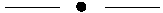
\includegraphics{fig/separator.pdf}
%	\end{center}
%\vfill
}

% Commands for semantic styling
\newcommand{\method}[1]{\texttt{#1}}
\newcommand{\mapkey}[1]{\texttt{#1}}
\newcommand{\datatype}[1]{\texttt{#1}}
\newcommand{\sampok}{\mapkey{samp.ok}}
\newcommand{\samperror}{\mapkey{samp.er\-ror}}
\newcommand{\sampwarning}{\mapkey{samp.warn\-ing}}
\newcommand{\sampresult}{\mapkey{samp.re\-sult}}
\newcommand{\sampstatus}{\mapkey{samp.sta\-tus}}
\newcommand{\sampmtype}{\mapkey{samp.mtype}}
\newcommand{\sampparams}{\mapkey{samp.pa\-rams}}
\newcommand{\stringtype}{\datatype{string}}
\newcommand{\listtype}{\datatype{list}}
\newcommand{\maptype}{\datatype{map}}
\newcommand{\sampint}{\datatype{SAMP int}}
\newcommand{\sampbool}{\datatype{SAMP bool\-e\-an}}
\newcommand{\sampfloat}{\datatype{SAMP float}}


% Commands/macros for VO protocol resumes
\def\semicolon{ semicolon (\texttt{;})}
\def\comma{ comma (\texttt{,})}
% \def\stringt{ \texttt{string} }
% \def\intt{ \texttt{integer} }
% \def\doublet{ \texttt{double} }

% Macros for XML tag and tags:

\newcommand{\xmlattr}[1]{\texttt{#1} at\-trib\-ute}
\newcommand{\xmlopen}[1]{\texttt{<#1>}}
\newcommand{\xmlclose}[1]{\texttt{</#1>}}
\newcommand{\xmlself}[1]{\texttt{<#1/>}}
\newcommand{\xmlenclose}[2]{
	\xmlopen{#1}\texttt{#2}\xmlclose{#1}
}
\newcommand{\xmlencloseattr}[3]{
	\xmlopen{#1 #2}\texttt{#3}\xmlclose{#1}
}
\newcommand{\xmltag}[1]{\xmlopen{#1} tag}
\newcommand{\xmltags}[1]{\xmlopen{#1} tags}
\newcommand{\dtdelement}[1]{\texttt{<!ELEMENT #1>}}
\newcommand{\dtdattlist}[1]{\texttt{<!ATTLIST #1>}}
\newcommand{\oxygenxml}[0]{
	Generated with the XML Schema diagram generator of the oXygen XML
	Editor.
}

\newenvironment{attributedquotenv}{
	\epigraphposition{flushright}
	\epigraphtextposition{flushleftright}
	\epigraphsourceposition{flushright}
	\setlength{\epigraphwidth}{0.6\textwidth}
	\setlength{\parindent}{1em}
}

\newcommand{\attributedquote}[2]{
	\begin{attributedquotenv}
		\epigraph{#1\hspace*{\fill}}{\emph{#2}\hspace*{\fill}}
	\end{attributedquotenv}
}
% The \hspace*{\fill} parts are needed in order to avoid
% the 

%Superscript and subscript commands, with common endings
%\newcommand{\superscript}[1]{\ensuremath{^{\textrm{#1}}}}
%\newcommand{\textsubscript}[1]{\ensuremath{_{\textrm{#1}}}}
\newcommand{\thsup}[0]{\textsuperscript{th}}
\newcommand{\stsup}[0]{\textsuperscript{st}}
\newcommand{\ndsup}[0]{\textsuperscript{nd}}
\newcommand{\rdsup}[0]{\textsuperscript{rd}}

\newcommand{\water}{\ensuremath{\textrm{H}_2\textrm{O}}}

%\newcommand{\classname}[1]{\fontencoding{OT1}\fontfamily{cmss}\fontseries{m}\fontshape{n}\fontsize{12}{15}\selectfont#1\normalfont}
%\newcommand{\classname}[1]{\textsf{#1}}
\newcommand{\classname}[1]{#1}

\newcommand{\ttmath}[1]{$\mathtt{#1}$}
\newcommand{\ucd}[1]{\texttt{UCD}$\mathtt{=}$\texttt{#1}}
\newcommand{\ttequals}[2]{\texttt{#1}\texttt{=}\texttt{#2}}

% Listings: Renew command \lstlistlistingname to change name into Spanish
\renewcommand{\lstlistlistingname}{Índice de listados}
\lstset{
	basicstyle=\tiny\ttfamily
}

% Hyphenation commands
\hyphenation{da-ta-base}
\hyphenation{da-ta-ba-ses}
\hyphenation{ex-tra-ga-lac-tic}


% To build the glossary
% \makeglossary
%\glossary{ALMA}
{
    	the \emph{Atacama Large Millimetre Array} is going to be the
        largest radio interferometer in the world. It will consist of
        more than 56 12-m diameter antennas in different
        configurations, together with a compact array of 8 6-m antennas
        and four more 12-m antennas to allow for smaller baselines
        (below 12m), allowing for much more extended emission to be
        captured. The antennas will be above 5000m in plateau of
        Chajnantor, at the Atacama desert, while the operation support
        facilities will be found just below 3000m.
}

\glossary{AMIGA}
{
    	bilingual acronym which stands in English for \emph{Analysis of
        the interstellar Medium of Isolated GAlaxies}, and in Spanish
        for \emph{Análisis del Medio Interestelar de Galaxias
        Aisladas}. AMIGA is a research project funded by the Spanish
        National Call for Space and Astrophysics wich started in 2004
        [TODO search this date], whose PI is Lourdes Verdes-Montenegro,
        devoted to the study of the largest optically selected sample
        of isolated galaxies (1050), following strict isolation
        criteria, in order to provide a baseline that can be used to
        differentiate whether particular galactic traits are intrinsic,
        or depend on the interaction with neighbouring galaxies. This
        study uses multi-wavelength information from many different
        telescopes and wave bands, and joined the \gls{SVO} in 2005
        in order to create \gls{VO} tools needed for performing
        AMIGA's work, but also useful for the community at large. AMIGA
        VO actitivies have a strong emphasis on the radio band, both
        because of our interest in \gls{ALMA}, and because of the
        relative under-development of the radio-VO, both in terms of
        number of archives, available tools, and data models.
}

\glossary{API}
{
    	acronym standing for \emph{Applications Programming Interface}.
        An API is a set of related functions that allow applications to
        make use of the operating system (or specific functions). For
        instance, in UNIX-like systems, the POSIX API is the one
        allowing file access, memory management, multi-tasking, et
        cetera. Programs written using the POSIX API do not need to
        implement file access, memory management, and so one, but
        instead they will call functions of the POSIX API suitable for
        those tasks.
}

\glossary{Applications Working Group}
{
    	The \gls{IVOA} Applications Working Group is concerned
        primarily with the software tools that astronomers use to
        access VO data and services for doing astronomy. This WG
        provides a means for VO Applications development and
        implementation to be closely linked to the standards
        development in the IVOA, and where necessary proposes and
        develops standards for VO Applications to interoperate. The
        role of the Applications WG is to identify missing or desirable
        technical capabilities for VO applications, as well as
        components in terms of scientific usability. This WG is the
        IVOA front-end for announcing and discussing new VO
        applications and standards for application interoperability.
        The \gls{PLASTIC} protocol was the first attempt at tool
        interoperability, and now the WG is promoting \gls{SAMP},
        which is still a \gls{Working Draft}.
}

\glossary{ASCII}
{
    	acronym standing for \emph{American Standard Code for
        Information Interchage}. ASCII is the standard for the
        codification of textual data in binary form. In only specifies
        the first 127 characters out of the 256 that can be encoded
        with one byte (2^8), and it can only properly show characters
        from the US-English alphabet and symbols. Other European
        characters, such as ñ, ç, ß, å, and the like are not covered by
        ASCII, and require additional encoding. As ASCII specifies 8
        bits per character, no single encoding can provide all
        characters from each different language, much less at the same
        time. The present solution for character interoperability is
        \gls{Unicode}.
}

\glossary{AstroGrid}
{
    	UK research program devoted to the exploitation of grid
        capabilities in the astronomical enviroment. Since the creation
        of the Astrophysical Virtual Observatory (AVO) prototypes,
        AstroGrid has focused on \gls{Virtual Observatory}
        interoperability of remote services, under what is called
        Global Worker Services, and the Common Execution Architecture.
        They also develop the VODesktop and the AstroRuntime. The
        latter is a set of functions for VO access that can be called
        either using \gls{XML-RPC} or \gls{Java-RMI} from any
        other application, while the former is a set of VO
        visualisation and data access and filtering tools built on top
        of the \gls{AstroRuntime}.
}

\glossary{AstroRuntime}
{
    	the AstroRuntime is an \gls{AstroGrid} subproject that tries to
        provide a complete \gls{\gls{Virtual Observatory}} toolbox to
        any application able to communicate with it. Technically, it is
        a client-side middleware that provides uniform access to all
        \gls{Virtual Observatory} services, from any programming
        language supporting \gls{XML-RPC} calls, direct \gls{HTTP}
        communications, or \gls{Java-RMI} interfaces.
}

\glossary{Astronomy}
{
		several dictionaries define \emph{astronomy} as the study of
        the properties of objects and matter outside the Earth's
        atmosphere. Etymologically, comes from the greek
        $\alpha\sigma\tau\epsilon\rho{}i$
		% αστέρι
        (\emph{astro-asteri}, meaning star), and the greek $\nu\'o\mu
        o\varsigma$
		% νόμος
		(\emph{nomos}, meaning law), and that would
        be the study of the laws governing celestial objects. If those
        laws are restricted to the relative movement of astronomical
        objects, is considered a part of Mathematics. However, when
        scientists try to derive physical or chemical properties from
        celestial objects, it is used interchangeably with
        \gls{astrophysics}.
}

\glossary{Astrophysics}
{
    	the part of \gls{astronomy} dealing with the acquisition of
        physical information from astronomical objects. Examples of
        such information include object velocities, distances,
        oscillations, temperatures, object dynamics, et cetera.
        However, many people use astronomy and astrophysics
        interchangeably, as today it is very difficult to perform
        non-physical astronomical observations, as even when measuring
        object positions and distances physical models are used to
        enhance the distance estimation.
}

\glossary{Attribute}
{
    	in \gls{XML}, an attribute is information that qualifies a tag,
        and goes alongside with it. For instance, \texttt{PARAM}
        \gls{tags} in a \gls{VOTable} can have \texttt{ID},
        \texttt{unit}, \texttt{datatype}, \texttt{precision},
        \texttt{width}, \texttt{ref}, \texttt{name}, \texttt{ucd},
        \texttt{utype}, \texttt{arraysize} and \texttt{value}
        attributes. Some attributes might be required for a particular
        tag. For instance, \texttt{PARAM} tags require an \texttt{ID},
        a \texttt{name}, and a \texttt{value}, making the minimum valid
        \texttt{PARAM} tag: \texttt{<PARAM name=``resolution''
        value=``50'' />}. Of course, \texttt{units} and \texttt{ucd}
        are not required attributes (in the sense that the VOTable XML
        schema does not define them as required), but are absolutely
        required to understand the quantity: \texttt{<PARAM
        name=``resolution'' value=``50'' units=``arcsec''
        ucd=``pos.angResolution'' />}).
}

\glossary{Batch processing}
{
    	Non-interactive processing of a bunch of data (\emph{batch}).
        Typically used for lengthy operations on the same set of data,
        and launched from a \gls{CLI}. Involves programming the series
        of operations, either with a script, or a complete application
        or tool. Batch processing is useful when processing different
        data sets with the same parameters, in order to obtain
        consistent results. Compare with \gls{Interactive session}.
}

\glossary{Binary-based file formats}
{
    	a binary-based file format is one where the data representation
        closely resembles the in-memory representation for programs
        doing computations with such data. Usually, binary-based file
        formats perform better at reading and writing, because there is
        no need to parse the input. However, binary-based file formats
        suffer from flexibility problems, and scripting tools need to
        decode the data first in order to manipulate them. Compare with
        \gls{text-based file formats}.
}

\glossary{Browser}
{
    	In computer science, a browser is a piece of software that
        allows navigating around, and perusing, a particular kind of
        information, such as \emph{Web browsers} for accessing the
        \gls{World Wide Web}, or \emph{file browsers} for navigating
        around a computer's file system.
}

\glossary{Character encoding}
{
    	The mapping between a particular sets of bits and a particular
        character printed or shown on screen is called character
        encoding. The best known encoding is \gls{ASCII}, but it fails
        to represent non-US-English characters, as it only specifies
        127 characters out of 256. The ISO provides character encoding
        specifications such as Latin1 for Western European countries,
        Latin2 for cyrillic, and the family of ISO 8859 standards for
        Arabic, Hebrew, Greek, and many other languages. Even different
        manufacturers used different encodings, such as IBM's EDBIBC,
        or Apple's MacRoman. The problem with ASCII based character
        encoding is that each encoding is exclusive: a Latin2 document
        cannot provide Arabic text, nor can Arabic and Hebrew be mixed,
        for instance. The solution consists in breaking the 256
        characters limit, and providing consistent support across
        operating systems, languages and scripting systems, from an
        international consortium. See \gls{Unicode}.
}

\glossary{CLI}
{
    	acronym for \emph{Command Line Interface}. A CLI is a
        text-based interface, similar to a UNIX shell, where commands
        are entered with a keyboard, and parameters are entered
        together with the command for batch processing sessions, or
        after entering the command for interactive processing sessions.
        Compare with \gls{GUI}.
}

\glossary{CSIC}
{
    	Spanish acronym standing for \emph{Consejo Superior de
        Investigaciones Científicas}, or \emph{High Council of
        Scientific Research} in English. CSIC is the largest research
        organisation in Spain, and the \gls{IAA} belongs to it.
}

\glossary{CSS}
{
    	acronym standing for \emph{Cascading Style Sheets}. CSS is a
        \gls{W3C} standard to define presentation by means of a
        hierarchical cascade of style sheets —similar to styles in word
        processing packages—, so that a given \gls{HTML}/\gls{XHTML}
        document content can show different appearances depending on
        the style sheet being applied.
}

\glossary{CSV}
{
    	A \gls{text-based file format} (compare with \gls{binary file
        formats}) where data records are separated in different rows
        (i.e., the text line separator acts as record separator), and
        data belonging to different columns are separated by commas
        (CSV stands for \emph{Comma Separated Values}). Optionally, the
        last row of comments prior to the first row of data can contain
        table headers. Compare with \gls{TST}.
}

\glossary{Data Access Layer Working Group}
{
    	The task of the Data Access Layer (DAL) working group is to
        define and formulate VO standards for remote data access.
        Client data analysis software uses these services to access
        data via the VO framework; data providers implement these
        services to publish data to the VO. The DAL working group will
        define the scope of the DAL standards, outline a process by
        which DAL standards are defined, and generate the initial
        version 1.0 of the DAL standard. This standard will provide
        guidance to data centres and survey projects when designing VO
        compliant interfaces. It will allow them to justify the
        allocation of resources for its implementation and maintenance.
        Once the work on Version 1.0 is accomplished the working group
        will coordinate future development of the standard. Currently,
        one \gls{IVOA} \gls{Recommendation} from this WG exists:
        \gls{SSAP}, and \gls{SCS}. \gls{SIAP} should follow soon, but
        it is still a \gls{Working Draft}.
}

\glossary{Data Modelling Working Group}
{
    	The role of the Data Modeling working group (WG) is to provide
        a framework for the description of \gls{metadata} attached to
        observed or simulated data. The WG activity focuses on logical
        relationships between these metadata, examining how an
        astronomer wants to retrieve, process, and interpret
        astronomical data, and providing an architecture to handle
        them. This WG standards can then be re-used in the protocols
        defined by the \gls{Data Access Layer Working Group} or in
        VO-aware applications.
}

\glossary{DOI}
{
    	Acronym for \emph{Digital Object Identifier}. A DOI consists of
        a permanent identifier given to an electronic document that, in
        contrast to a \gls{URL}, is not dependent upon the electronic
        document's location. A DOI has to be resolved by the
        [http://doi.org/ DOI System], which provides both the metadata
        associated with the document, and a known location for an
        electronic copy. DOIs are particular cases of the CNRI Handle
        System, the first system for resolving digital document codes
        into URLs. DOIs are CNRI Handles with prefix \texttt{10}.
        Compare with \gls{URN}s.
}

\glossary{Driver}
{
    	In computer technology, a driver is a piece of software in
        charge of talking to classes of devices, so that an application
        only has to talk to the class of devices, and the difference in
        detail between different devices is abstracted by the driver.
        For instance, \gls{JDBC} drivers provide database connectivity
        for applications written in \gls{Java}, and hide the
        implementation differences between different database vendors,
        such as MySQL or PostgreSQL.
}

\glossary{DTD}
{
    	acronym standing for \emph{Document Type Definition}. DTD is a
        non-XML-based purpose-specific language for the definition of
        constraints for \gls{XML} documents, also known as \gls{XML
        schema}. A DTD document specifies the \gls{tags} that can be
        used in documents using a particular DTD, tag \gls{attributes},
        tag values, and the order, repetition, and hierarchical
        relationship between tags. Compare with \gls{XML Schema}. (Mind
        the capitalisation.)
}

\glossary{Dublin Core}
{
    	set of \gls{metadata} for archive resources shared by all
        registries which are \gls{OAI}-compliant. The Dublin Core
        mandates metadata keywords for resource titles, creators,
        subject, description, publishers, contributors, publishing
        data, resource type, resource format, resource identifiers,
        resource sources, language, relationships with other resources,
        resource coverage, and resource-related rights.
}

\glossary{End-point}
{
    	in \gls{web services} parlance, an end-point is an \gls{URL} to
        which \gls{REST} or \gls{SOAP} conforming queries can be
        performed. End-points for web services are usually defined via
        \gls{WSDL} documents, whereas for \gls{VO} services end-points
        are defined in the VO \gls{Registry}.
}

\glossary{Euro3D}
{    	\gls{FITS}-based data format developed within the \gls{OPTICON}
        network for storing 3D spectra coming from \gls{IFU}s. It can
        be made general enough to hold data coming from radio
        interferometry data, but the overhead becomes enormous compared
        to more traditional FITS-based ways of storing this data.
}

\glossary{FITS}
{
    	acronym standing for \emph{Flexible Image Transport System}.
        FITS is a file format standard developed by NASA in the '70s,
        which allows for metadata headers (\emph{cards}) of the form
        \texttt{KEYWORD = VALUE}, and arbitrary shaped binary tables
        for which column number and column descriptions exist in the
        headers. FITS keywords are made of at most 8 ASCII characters,
        and the whole keyword, equal separator (\texttt{=}), and value,
        cannot be more than 79 characters long. FITS files are
        organised around HDUs (Header Data Unit), described by the
        primary FITS header, which in turn can contain additional
        headers and HDUs. Only a few FITS headers are standardised.
}

\glossary{FORTRAN}
{
    	acronym for \emph{FORmula TRANslator}. FORTRAN is a programming
        language invented by John Backus in the '50s for IBM, and has
        an special emphasis on matrix computations, for which is best
        suited. This native support of vectors, arrays, and matrices
        made FORTRAN the most popular programming language in the
        scientific world. As many of the astrophysical and
        astrometrical calculations make extensive use of this kind of
        processing, FORTRAN soon became the preferred programming
        language in astrophysics.
}

\glossary{GDL}
{
    	acronym for \emph{GNU Data Language}. GDL is an
        \gls{open-source} clone of the \gls{IDL} language, without the
        IDL libraries. It can be used to perform data analysis
        operations using IDL compatible libraries, such as the \gls{IDL
        Astronomy Library}.
}

\glossary{Grid and Web Services Working Group}
{
    	The aim of the \gls{IVOA} Grid & Web Services Working Group is
        to define the use of \gls{grid} technologies and \gls{web
        services} within the VO context and to investigate, specify,
        and implement required standards in this area. This group was
        formed from a merger of the previously existing Web Services
        group and the Grid group, as ordered at the IAU General
        Assembly in 2003.
}

\glossary{Grid}
{
		Grid computing is a form of distributed computing, where
        computation and/or storage nodes from a pool of geographically
        distributed resources can be used to perform tasks in parallel,
        with more or less interaction between nodes, and which use
        common \gls{middleware} that provides the resource allocation
        \gls{API}s to grid computing applications. A grid can be
        functionally defined as a system of computers without a
        centralised administration, which communicate by means of open
        standards, and which provide a quality of service beyond
        \emph{best effort} (i.e., programs in the grid are launched on
        suitable nodes, abnormal program termination events are logged
        and execution retried, and needed execution times can be
        specified).
}

\glossary{GUI}
{
    	Acronym for \emph{Graphical User Interface}. A GUI is a
        graphical way to show data on a computer screen, and perform
        user interaction with graphical devices, as mouse-controlled
        pointers for interacting with on-screen buttons. GUIs are also
        useful for \gls{interactive sessions}, such as interactive
        visualisations where the graphical representation can change
        interactively following user inputs. Example of GUI
        environments are the X-Window environment for general computing
        tasks, the IDLDE, or IRAF's graphical xgterm windows. Compare
        with \gls{CLI}.
}

\glossary{HTML}
{
    	The \emph{Hyper Text Markup Language} is the main invention of
        Tim Berners-Lee, and is the cornerstone of the \gls{World Wide
        Web}. HTML uses \gls{tags} to markup (i.e., to label) text
        content, specifying both content, links, and presentation. The
        latest HTML versions, and \gls{XHTML}, try to provide content
        with markup that provides semantics to the content, while the
        presentation is left to CSS.
}

\glossary{HTTP}
{
    	The \emph{Hyper Text Transfer Protocol} is the other invention
        and cornerstone of the \gls{World Wide Wed}, and was also
        invented by Tim Berners-Lee. HTTP initially was a protocol for
        hypertext data retrieval, allowing for GET operations on
        \gls{URL}s pointing to HTML documents, or hypermedia elements
        pointed by the HTML documents such as images, sounds, videos,
        et cetera.
		It was later upgraded to allow information transport from
        the browser to the server, via HTTP POST calls which sent
        information from web forms, and additional PUT and DELETE calls
        for better semantic support of remote operations. This protocol
        is also used for the query of web services, which must provide
        an HTTP server.
}
\glossary{Hypermedia}
{
    	See \gls{hypertext}.
}

\glossary{Hypertext}
{
    	term coined by Ted Nelson in 1965, at the same time as
        hypermedia, when developing a collaborative document editing
        that allowed text and media insertion and labelling, with links
        between document sections in the same or another document. Ted
        Nelson work can be seen as an implementation of Vannevar Bush
        vision as expressed in his 1945 essay \emph{As we may think}.
        For instance, in a text dealing with web services, links may
        exist to terms such as \gls{HTTP}, \gls{XML}, \gls{REST},
        \gls{SOAP}, \gls{WSDL}, et cetera,
		which would be placed exactly where
        those terms appeared. Such a \emph{link-enriched} text is
        called hypertext. If the system goes beyond text to use other
        kinds of media (graphics, images, sounds, video, et cetera) the term
        hypermedia is used.
}

\glossary{IAA}
{
    	Spanish acronym standing for \emph{Instituto de Astrofísica de
        Andalucía}, or \emph{Institute of Astrophysics of Andalusia}.
        Usually written as IAA-CSIC, to show the IAA is an institute
        belonging to the \gls{CSIC}.
}

\glossary{IAU}
{
    	The \emph{International Astronomy Union} was founded in 1919.
        Its mission is to promote and safeguard the science of
        astronomy in all its aspects through international cooperation.
        Its individual members are professional astronomers all over
        the world, at the Ph.D. level and beyond, and active in
        professional research and education in astronomy. Besides, the
        IAU maintains friendly relations with organisations that
        include amateur astronomers in their membership.
        http://www.iau.org/
}

\glossary{IDL}
{
    	acronym standing for \emph{Interactive Data Language}. The IDL
        is a language and \gls{CLI} environment for performing
        mathematical operations, with an emphasis on matrix algebra, on
        \gls{interactive sessions}. IDL has a strong share of computing
        the astronomy and astrophysics world due to its similarity to
        an interactive version of FORTRAN, and to the huge \gls{IDL
        Astronomy Library} providing packages for many astronomical and
        astrophysical \gls{reduction} duties. IDL is not open software,
        and initially belonged to Research Systems Inc. (RSI), and now
        belongs to ITT Industries and operates as ITT Visual
        Information Solutions). However, the Astronomy Library is
        \gls{open-source} software, and can be used with clones such as
        \gls{GDL}.
}

\glossary{IEC}
{
    	acronym for the \emph{International Electrotechnical
        Commission}, a non-profit international standards organisation
        that prepares and publishes International Standards for all
        electrical, electronic, and related technologies. IEC also
        manages conformity assessment, in order to certify that
        equipment complies with its standards.
}

\glossary{IETF}
{
    	The \emph{Internet Engineering Task Force} develops and
        promotes Internet standards, co-operating closely with the
        \gls{W3C} and \gls{ISO}/\gls{IEC} standard bodies and dealing
        in particular with standards of the \gls{Internet}
        \gls{protocol suite}. It is an open standards organisation,
        with no formal membership or membership requirements.
        \gls{IVOA}'s organisation is loosely modelled after the IETF's,
        as their goals a very similar: promote open, interoperable
        standards to be used throughout the Internet.
}

\glossary{INTA}
{
    	Spanish acronym standing for \emph{Instituto Nacional de
        Técnica Aeroespacial}, or \emph{National Institute for
        Aerospatial Technologies} in English. INTA is the organisation
        funding the \gls{LAEFF}, and ensures continued funding both for
        LAEFF and the \gls{SVO}.
}

\glossary{Interactive session}
{
    	Session of data processing which is performed in an environment
        that uses simple steps that return control to the user as soon
        as they have finished. Some of the steps might imply \gls{batch
        processing}, but after each step is finished control is
        returned to the user. The user has control of a particular
        environment, where data resides, and can directly make change
        to the data. Some \gls{CLI} environments for interactive
        processing are \gls{IRAF}, \gls{IDL}, \gls{Python}, \gls{shell}
        command lines, \gls{MATLAB}, et cetera.
		Typically, \gls{GUI}s are also
        useful for interactive sessions.
}

\glossary{IRAF}
{
    	acronym standing for \emph{Image Reduction and Analysis
        Facility}. IRAF is a huge collection of software modules
        written by astronomers and programmers at the \gls{NOAO},
        needed for the \gls{reduction} of astronomical images provided
        as pixel matrices, such as those provided by imaging array
        detectors like CCDs. IRAF provides a \gls{CLI} that handles the
        loading of such images, mathematical operations on them such as
        image subtraction or division, with specific analysis tasks to
        extract scientific products such as 1D spectra, 2D spectra,
        pixel counts, etc, during \gls{interactive sessions}. Scripts
        can be written to perform \gls{batch processing}.
}

\glossary{ISO}
{
    	short-name of the \emph{International Organisation for
        Standardisation}, an international-standard-setting body
        composed of representatives from various national standards
        organisations. The form \emph{ISO} is used to avoid changing
        the organisation name in different languages, and comes from
        the Greek $i\sigma{}o\varsigma$ (\emph{isos}),
        meaning \emph{equal}. The ISO sanctions international
        standards. In the case of standards dealing with information
        technologies, there is a Joint Technical Committee with
        \gls{IEC}, and standards coming from that joint committee are
        known as ISO/IEC standards.
}

\glossary{IVOA}
{
    	acronym standing for \emph{International Virtual Observatory
        Alliance}. An alliance of different national \gls{Virtual
        Observatory} initiatives, formed in June 2002, whose mission is
        to facilitate the international co-ordination and collaboration
        necessary for enabling global and integrated access to data
        gathered by astronomical observatories. The IVOA Executive is
        present at the \gls{IAU} via the Virtual Observatory Working
        Group. http://ivoa.net/
}

\glossary{IVORN}
{
    	acronym standing for \emph{International Virtual Observatory
        Resource Name}. An IVORN is a kind of \gls{URN} with protocol
        \texttt{ivo:}, that encodes both an \emph{Authority ID} and a
        \emph{Resource Key} within that particular authority. The
        encoding is such that the URN is of the form
        \texttt{ivo://AuthorityID/ResourceKey}. An additional parameter
        can be specified for particular, local uses, after either a
        question mark (\texttt{?}) or a number mark (\texttt{#}). Thus,
        the URN \texttt{ivo://AuthorityID/ResourceKey#temp1}
        corresponds to an IVORN (protocol \texttt{ivo://}) for a
        \texttt{ResourceKey} resource under \texttt{AuthorityID}, and
        #temp1 is a particular reference of local value (for instance,
        in order to specify message dates). IVORNs are an \gls{IVOA
        Recommendation}. \emph{Authority ID}s must be registered as
        \gls{VO Resource}s of type \emph{identity}.
        http://www.ivoa.net/Documents/latest/IDs.html
}

\glossary{Java}
{
    	Platform-independent programming language developed by Sun
        Microsystems with the aim of writing applications that can work
        across different computing platforms by means of a \gls{Virtual
        Machine} that executes compiled Java byte-code, and isolates
        the differences between operating systems. In the context of
        the \gls{Virtual Observatory}, many tools are being written in
        Java so that they can reach the maximum number of potential
        users, regardless of platform. http://www.java.com/
}

\glossary{Java-RMI}
{
    	short for \emph{Java Remote Method Invocation}, Java-RMI is an
        \gls{API} that provides \gls{RPC} capabilities within the
        \gls{Java} object model. In other words, it allows Java objects
        remotely call methods from objects in other packages, without
        the burden of setting up a whole RPC server, because Java-RMI
        is embedded in the language.
}

\glossary{JDBC}
{    	\emph{Java Data Base Connectivity} is a standard way of
        specifying connections to \gls{SQL}-compliant databases, so
        that an application written in \gls{Java} uses the same
        database query source code, and only the configuration of the
        JDBC driver is different.
}

\glossary{LAEFF}
{
    	Spanish acronym for \emph{Laboratorio de Astrofísica Espacial y
        Física Fundamental}, or \emph{Spatial Astrophysics and
        Fundamental Physics Laboratory} in English. LAEFF is the seed
        of the \gls{SVO}, and was the first organisation to develop a
        \gls{VO} compliant archive (INES) for the newly extracted
        spectra from the IUE mission. LAEFF belongs to \gls{INTA}.
}

\glossary{Markup}
{
    	As a noun, refers to textual labels (\gls{tags}) that are
        applied to parts of data to specify either different visual
        representations, particular data semantics, or classification
        within a hierarchy. Examples of markup are \gls{XHTML} tags,
        which either specify visual properties (i.e, \texttt{<b>} for
        boldface, or \texttt{<i>} for italics), hierarchical
        relationships (i.e., \texttt{<h1>} to \texttt{<h6>} to
        represent headers within a document outline), or semantics
        (again, \texttt{<hn>} to represent headers, \texttt{<ol>} to
        represent ordered lists or dictionary entries, or
        \texttt{<abbrv>} for abbreviations). In some languages, markup
        is used to mark the start and end of applicability of the tags,
        while in others they only mark the start, and the end is
        implicit in the language, such as LaTeX' section hierarchy
        using \texttt{\part}, \texttt{\chapter}, \texttt{\section} and
        related commands.
}

\glossary{Metadata}
{
    	data about the data, or additional information describing the
        actual data. For instance, in a \gls{FITS} file, headers
        provide metadata via several keywords, in order to specify
        telescope (\texttt{TELESCOP}), instrument (\texttt{INSTRUME}),
        date of observation (\texttt{DATEOBS}), et cetera. Metadata is
        usually not needed if the \emph{system} performing the
        observation is the same as the one performing the reduction, as
        data \gls{reduction} procedures can be built with direct
        knowledge of the observing conditions. However, if data are to
        be treated by a different system, they need the additional
        metadata so that all system configuration is made explicit.
        Metadata scope can be just a single datum, a data table, a data
        file, or a complete file collection. In the \gls{VO}, metadata
        is split into several data models, which specify what kinds of
        metadata are needed, for instance, for observing target
        specification, astronomical data characterisation in different
        domains, et cetera.
}

\glossary{Method}
{
    	Part of an objects that contains code to perform a function.
        See \gls{Property}.
}

\glossary{Middleware}
{
    	is the software layer that lies between the operating system
        and applications on each side of a distributed computing system
        in a network. In the case of \gls{grid computing}, middleware
        manages access to remote storage elements, the replication of
        local archives into the grid storage pool, job submission and
        control, et cetera.
}

\glossary{Model}
{
    	See \gls{MVC}.
}

\glossary{Moore's Law}
{
    	Named after Intel's engineer Gordon Moore, this \emph{law}
        should be better known as \emph{Moore's Observation}. Moore
        observed the number of transistors that different integrated
        chips fabrication facilities where able to integrate on a
        single chip on different moments since the invention of the
        integrated circuit, and saw that they fitted an exponential
        law, where the number of transistors per chip doubled each
        year. The exponential increase in integrated transistors is
        followed independently by different equipment at different
        rates: computer memories show the highest transistor densities,
        doubling every [TODO find rate], while microprocessors double
        every 18-24 months.
}

\glossary{MVC}
{
    	acronym standing for \emph{Model-View-Controller}, a
        programming paradigm that advocates the separation between
        \gls{Models} (the internal data representation), \gls{Views}
        (the way the information gets to the user, and the user
        interface users can act upon), and \gls{Controllers} (the
        intermediate layer between Model and Views.
}

\glossary{NOAO}
{
    	Acronym standing for \emph{National Optical Astronomy
        Observatory}, organisation for the management of the US
        National Solar Observatory, the Inter-American Observatory at
        Cerro Tololo, and the Kitt Peak National Observatory, together
        with the US participation in the Gemini Observatory. The NOAO
        is responsible for astronomical archives for all managed
        observatories.
}

\glossary{OAI}
{
    	acronym standing for \gls{Open Archives Initiative}.
}

\glossary{Object (computing)}
{
    	an object, in computer science, is either a blueprint for
        building useful computer constructs which tie together
        operations and data on which those operations are to be
        performed, or an instance of such computer construct built
        following that blueprint. Objects have properties and methods,
        and both properties and methods can only be used by the same
        object, by other objects of the same blueprint, by other
        objects which have parts of their blueprint in common, or by
        any other object, depending on the scope we have defined both
        for the object and its particular properties and methods.
}

\glossary{Open Archives Initiative}
{
    	a non-profit organisation which develops and promotes
        interoperability standards that aim to facilitate the efficient
        dissemination of content. It has roots in the Open Access
        Movement, but over time its role has expanded to promote broad
        access to digital resources of all kinds for \gls{e-Learning}
        and \gls{e-Science}. The VO \gls{Registry} uses OAI's
        harvesting protocol (OAI-PMH) for data interchange between
        Registries.
}

\glossary{OPTICON}
{
    	acronym standing for \emph{OPTical and Infrarred COordination
        Network}. OPTICON's objective is to standardise astronomical
        procedures (regarding both data acquisition and manipulation,
        including software packages) as much as possible between the
        \gls{optical} and the \gls{IR} bands. OPTICON funding comes
        from European Commission's Framework Programmes. [TODO review
        this is correct]
}

\glossary{Parser}
{
    	part of program code devoted to interpret (parse) user or file
        input. Parsers differ for different applications, but they
        usually cope with finding data delimiters, converting text
        representations into machine representations, and giving access
        to particular pieces of data.
}

\glossary{Pipeline}
{
    	In software engineering, a pipeline consists of a chain of
        processing elements (processes, threads, coroutines, et cetera),
        arranged so that the output of each element is the input of the
        next. In astronomy, a pipeline is the chain of processes that
        need to be performed on an astronomical observation in order to
        derive one or more scientific products.
}

\glossary{PlasKit}
{
    	implementation written in \gls{Java} of the \gls{PLASTIC}
        protocol developed by Mark Taylor for his \gls{TOPCAT}
        application. It implementsts both the PLASTIC hub, and PLASTIC
        client classes.
}

\glossary{PLASTIC}
{
    	Acronym of \emph{PLatform for AStronomical Tool
        InterConnection}, a protocol for communication between
        client-side \gls{Virtual Observatory} astronomy applications.
        Applications use PLASTIC to perform tasks such as instruct
        other PLASTIC-enabled applications to load \gls{VOTables},
        highlight a subset of rows or load an image of a particular
        area of sky. PLASTIC allows a modular approach to choosing VO
        applications, where each application is used for the task it
        performs best. There are two kinds of PLASTIC applications:
        Application hubs, and client applications. Client applications
        register themselves with the PLASTIC hub, and use the hub to
        query for other registered applications, and the PLASTIC
        services those applications provide.
}

\glossary{Product\gls{, }Data Product\gls{
 or }Scientific Product}
{
    	a processed observation product in the form of an image,
        spectrum, set of spectra, flux measurement, et cetera, that it
        is calibrated and compensated for all instrumental and
        observational effects. Synonym of \emph{reduced data}.
}

\glossary{Property}
{
    	Part of an object devoted to store pieces of information. Those
        properties are accessible to object methods, and can be made
        invisible to other objects, so that particular object method's
        can perform their tasks based on their properties, while
        (usually) not accessing other object properties. In \gls{XML},
        the names property and attribute are used ambiguosly.
}

\glossary{Proposed Recommendation}
{
    	Within \gls{IVOA}, a Proposed Documentation is a document that,
        after starting as a Working Draft, has received sufficient
        input from the \gls{Working Group} (WG), possibly with a
        WG-wide \gls{RFC} period, and has not suffered a significant
        revision after the RFC.
}

\glossary{Protocol}
{
    	Set of standard rules for data representation, signalling,
        authentication and error detection required to send and
        retrieve information over a communications channel. In the
        context of the \gls{IVOA}, a protocol regulates how to retrieve
        information from a \gls{Virtual Observatory} service, and
        depends on the kind of information being provided. Astronomical
        images are available through servers conforming to the
        \gls{SIAP} protocol, whereas the spectral information is made
        available through the \gls{SSAP} protocol.
}

\glossary{Python}
{
    	Name of a computer programming and scripting language,
        developed by Guido van Rossum in 1991, and available under an
        \gls{Open Source} license for many different computer
        platforms. Python programs are compiled at execution time, and
        the compiled code is executed by the interpreter. Python has
        been widely adopted in the astronomical community, and its
        \gls{XML-RPC} and \gls{web services} capabilities allow for
        interoperation with a large basis of services written in any
        language that supports \gls{XML-RPC}, and with \gls{Virtual
        Observatory} web services, making it a suitable candidate for
        interoperation with Java and the Virtual Observatory.
}

\glossary{Recommendation}
{
    	Within \gls{IVOA}, a document which is in the Recommendation
        state has already reached the \gls{Proposed Recommendation}
        stage, has passed an IVOA-wide four weeks RFC period without
        significant revisions, the Chair of the corresponding
        \gls{Working Group} has asked the IVOA Chair to promote the
        document, and the \gls{IVOA Executive} has sanctioned the
        document to \gls{Recommendation}. If the Recommendation is
        relevant enough, the IVOA Executive might send the document to
        the joint IAU VO Working Group to obtain the endorsement of the
        \gls{IAU}, and reach the state of \gls{IAU Standard}.
}

\glossary{Reduction}
{
    	in astrophysics parlance \emph{reduction}, or more precisely
        data reduction, refers to the operations needed to convert raw
        data coming from astrophysical instruments into scientific
        products. For instance, the raw information coming from a radio
        spectrograph is the form of photon counts in different
        frequency channels. The astrophysicist also needs the usual
        photon count on the detector when the instrument observes an
        empty patch of the sky; the opacity of the atmosphere at
        different angles to correct for atmospheric extinction at the
        elevation of the source; the average photon count from a
        calibration source, so that received photon fluxes can be
        converted into photon fluxes emitted by the source; and the
        Doppler-effect correction due to the relative movements between
        the source and the observatory. The \emph{reduced} scientific
        products are flux and wavelength calibrated spectra, integrated
        flux within a waveband, and/or the recession velocity of an
        object relative to the Earth, our solar system, or our own
        galaxy.
}

\glossary{Registry}
{
    	In the \gls{Virtual Observatory} architecture, a Registry holds
        resource \gls{metadata} (in the form of a \gls{VOResource}
        record) for the different services available within the VO,
        allowing astronomers to locate, get details of, and make use
        of, any resource located anywhere. There is no \emph{prefered}
        IVOA registry, but instead registries are interoperable,
        allowing the \gls{harvesting} of records from one registry to
        another, so that eventually all registered services can be
        found in any other registry. Registries conform to the
        \gls{OAI} specifications, so that existing Registries for other
        digital repositories have been enhanded to be able to cope with
        VO records. This also means that VO registry records, VO
        Resources, use the \gls{Dublin Core} metadata for maximum
        interoperability.
}
 
\glossary{REST}
{
    	Computer acronym for \emph{REpresentational State Transfer}.
        REST is a collection of network architecture principles, first
        enunciated by Roy Fielding in his Ph.D. thesis, which outline
        how to define and address resources. REST architectures do not
        rely on \gls{HTTP} to keep the state of an interaction.
        Instead, the state is encoded in the service invocation, both
        in the kind of HTTP operation to be performed (GET for
        completely stateless calls, such as retrieving information from
        a particular user or resource; POST for operations that update
        existing resources; PUT for operations which add new resources;
        DELETE for operations which remove records), and a URL
        containing all information needed for resource identification,
        and additional data for resource filtering (GET) or updates
        (POST, PUT, DELETE). Both GET and POST operations, in an
        architecture following REST principles, can be repeated as many
        times as desired without side effects. PUT operations should
        also be called additional times, and the receiver has to be
        able to identify identical requests not as new resources, but
        resource modifications. And DELETE operations should provide an
        error when called more than once.
}

\glossary{RFC}
{
    	acronym standing for \emph{Request For Comments}. In \gls{W3C}
        parlance, an RFC is a document that states the current best
        practices, or recommended behaviour, for applications,
        protocols, and other interoperation tools, as well as best
        practices for the development of new practices. In the
        \gls{IVOA}, an RFC is issued for a document in \gls{IVOA
        Working Draft} status prior to become an \gls{IVOA Proposed
        Recommendation}.
}

\glossary{RPC}
{
    	acronym of \emph{Remote Procedure Call}. RPC is an
        inter-process communication technology that allows a computer
        program to cause a subroutine or procedure to execute in
        another environment (commonly on another computer on a shared
        network, or in another running application). In languages
        supporting RPC, the programmer does not have to specify the
        details for this remote interaction. More modern flavours of
        RPC are \gls{XML-RPC}, and \gls{Java-RMI}.
}

\glossary{SAMP}
{		\emph{Simple Application Messaging Protocol}, a local
		messaging protocol intented to replace \gls{PLASTIC}, in
		order to avoid programming-language dependencies (parts of
		PLASTIC depended upon the Java specific RPC, Java-RMI), and
		to make protocol semantics richer and simpler. SAMP hubs
		exist in \gls{Perl}, \gls{Python} and \gls{Java}
		\invisiblenote{in alpha versions}, as well as clients,
		whereas true PLASTIC hubs only existed in Java. See
		\gls{PLASTIC} for comparison.
}

\glossary{SCS}
{
    	acronym standing for \emph{Simple Cone Search}, an \gls{IVOA}
        \gls{Recommendation} from the \gls{Data Access Layer}
        \gls{Working Group} that specifies how to perform positional
        queries catalogues of astronomical sources within a prescribed
        search radius around a central position, hence the term
        \emph{Cone Search}.
}

\glossary{SDSS}
{
    	is the acronym for the \emph{Sloan Digital Sky Survey}, a major
        multi-filter imaging and spectroscopic survey using a dedicated
        2.5-m wide-angle optical telescope at Apache Point Observatory
        in New Mexico. The project was named after the Alfred P. Sloan
        Foundation. The survey was begun in 2000, and aims to map 25%
        of the sky with wide-angle observations of around 6 square
        degrees in five filters (ugriz). The observations are processed
        through a dedicated pipeline that differentiates between stars,
        galaxies, and other kinds of objects, and is finally expected
        to provide a catalogue of 100 million objects, and spectra for
        1 million objects. The processing includes high-precision
        redshift determination from the spectroscopic observations, and
        more coarse photometric redshift estimation from the source
        intensity in the different filters.
}

\glossary{SED}
{
    	acronym for \emph{Spectral Energy Distribution}. In
        astrophysics, the SED is a function that gives energy per
        wavelength or frequency unit. In the \gls{VO}, SED is a data
        model --expressed as an \gls{XML} \gls{Schema}-- for such
        astrophysical spectral energy distributions, that can be also
        used to specify single frequency fluxes (continuum
        measurements).
}

\glossary{Semantics Working Group}
{
    	This \gls{IVOA} working group (WG) aims to systematise the way
        in which meaning is attributed to particular data or metadata
        fields within the VO. This WG started by specifying \gls{UCD}s,
        which provided broad physical meaning to quantities in generic
        \gls{VOTable}s. Later, it has expanded its scope to keep
        maintaining UCDs, but also specify an IVOA Standard Vocabulary,
        and the exploration of Semantic Web/Ontologies technologies
        within the Virtual Observatory.
}

\glossary{Serialisation}
{
    	Serialisation is the process of converting a set of different
        objects and entities, belonging to different data models, into
        a single, linearly accessible, document, in such a way that a
        univocal reconstruction of the serialised objects and entities
        is possible.
}

\glossary{SIAP}
{
    	acronym standing for \emph{Simple Image Access Protocol}. SIAP
        is a protocol specially crafted for the discovery and retrieval
        of astronomical images within the \gls{Virtual Observatory}.
        The SIAP is an \gls{IVOA} \gls{Working Draft} [TODO check], and
        is one of the IVOA's \gls{Data Access Layer} \gls{Working
        Group} protocols.
}

\glossary{SOAP}
{
    	acronym originally standing for \emph{Simple Object Access
        Protocol}. SOAP is a web services communication protocol which
        extends \gls{XML-RPC} with additional capabilities, such as
        support for different transports (i.e., SOAP could not only be
        used on \gls{HTTP}/HTTPS, but on \gls{SMTP}, and even instant
        messaging if a suitable transport layer were built). SOAP web
        services are usually described by a \gls{WSDL} document.
}

\glossary{SQL}
{
    	The \emph{Standard Query Language} is the most standardised way
        to query databases. It specifies database operations such as
        \texttt{SELECT} rows and columns, \texttt{INSERT} data into
        existing tables, \texttt{UPDATE} particular rows, or even
        \texttt{CREATE} the tables. When querying archives, the most
        usual SQL construct is the \texttt{SELECT}, which specifies
        which tables we want to obtain data \texttt{FROM}, and what
        conditions do the data conform to (\texttt{WHERE} is valid data
        in parameter space).
}

\glossary{SSAP}
{
    	acronym for \emph{Simple Spectrum Access Protocol}, a protocol
        devised after the \gls{SIAP}, and that allows for discovery and
        retrieval of instrumental or synthetic spectra within the
        \gls{Virtual Observatory}. The SSAP is an \gls{IVOA Working
        Draft}, nearing the status to \gls{IVOA Proposed
        Recommendation} [TODO check].
}

\glossary{Starlink Project}
{
    	 The Starlink project was a UK funded computing project which
         supplied general-purpose data reduction software. It was
         funded from 1980 by the Particle Physics and Astronomy
         Research Council, which withdrew funding in 2005. The Joint
         Astronomy Centre took over Starlink's software assets, with
         the latest software release dated February 2008.
}

\glossary{STIL}
{
		Acronym for \emph{Starlink Tables Infrastructure Library}.
		Developed by Mark Taylor for the \gls{Starlink project},
		the STIL is a pure \gls{Java} library for generic input,
		output, and processing of tabular data. It presents to the
		application programmer a view of a table which looks the
		same regardless of whether it came from a \gls{FITS} file,
		a \gls{VOTable}, an \gls{ASCII} text file, a query on a
		relational database, or whatever. It was initially
		developed to allow Java packages to deal with the Starlink
		table format, and has been enhanced to deal with VOTables.
}

\glossary{SVO}
{
    	acronym standing for \emph{Spanish Virtual Observatory}. The
        SVO is the organisation that represents VO efforts within
        \gls{IVOA} and the \gls{Euro-VO} since 2004. SVO is leaded by
        the VO and Archives group at the \gls{LAEFF-INTA}, and its PI
        is Enrique Solano. LAEFF-INTA provides most of the FTEs for the
        SVO, but the \gls{IAA-CSIC} also provides 1 FTE, belonging to
        the \gls{AMIGA} group.
}

\glossary{Tag}
{
    	Piece of metadata used to label a particular piece of data. In
        \gls{XML}, tags are enclosed between angular brackets
        (\texttt{<tag>}), and either surround a piece of data between
        corresponding start and end labels (e.g., in
        \gls{XHTML},\texttt{<p></p>} are used for paragraphs, as in
        \texttt{<p>This is a tagged paragraph</p>}), or are
        self-contained (e.g., in a \gls{VOTable}, common table
        parameters are defined as \texttt{<PARAM name=``Right
        Ascension'' ucd=``pos.eq.ra'' unit=``degrees'' value=``180.0''
        />}). Notice that tag semantics are provided (preferably) by
        the XML Schema, or the XML DTD if the XML document does not use
        an Schema.
}

\glossary{Text-based file format}
{
    	a text based file format is one where data is stored in a
        human-readable form, so that text manipulation tools (shell
        scripts, or UNIX tools such as \texttt{sed} and \texttt{awk},
		for
        instance) can deal with such files, at the expense of data
        retrieval speed. Programs which use text-based files need to
        parse the input in order to convert the text into an internal
        binary format suitable for manipulation. Please compare with
        \gls{binary-based file formats}.
}

\glossary{TOPCAT}
{
    	acronym standing for \emph{Tool for OPerations on CAtalogues
        and Tables}, and name of an application written in \gls{Java}
        developed by Mark Taylor for the \gls{Starlink project}. It
        provides an interactive graphical viewer and editor for tabular
        data, and uses the \gls{STIL} library as its internal table
        model. In the latest versions it has incorporated \gls{VO}
        capabilities, both by enhancing the STIL to deal with
        \gls{VOTables}, and by incorporating \gls{PLASTIC} (through the
        \gls{PlasKit}).
}

\glossary{TST}
{
    	Tab-separated text is a \gls{text-based file format} where
        records are separated by the text line separator, and fields
        are separated by tabs (\gls{ASCII} character \texttt{0x08}).
        Optionally, the last row of comments prior to the first row of
        data can contain table headers. Compare with \gls{CSV}.
}

\glossary{UCD}
{
    	acronym of \emph{Unified Content Descriptor}. UCDs are one of
        the attributes (meta-data) that table columns in the
        \gls{Virtual Observatory} can have. In particular, is one of
        the attributes for the \texttt{FIELD} and \texttt{PARAM} tags
        in a \gls{VOTable}. The UCD is built from a controlled
        vocabulary, managed by the \gls{IVOA Semantics Working Group},
        that provides physical semantics to the \texttt{FIELD} or
        \texttt{PARAM}eter using the UCD. There are two versions of the
        UCD standard: UCD1, which uses long strings of underscore (_)
        separated tags (e.g. \texttt{POS_EQ_RA}), and the newer,
        recommended, UCD1+, which consists of a series of atoms that
        can change or refine their meaning by juxtaposition. E.g.,
        \texttt{pos.eq.ra} indicates that some field provides the right
        ascension for a position in equatorial coordinates, while
        \texttt{pos.eq.ra; meta.main} indicates that for all the fields
        that might provide a right ascension, this is the main
        reference.
}

\glossary{Unicode}
{
    	international standard character encoding capable of holding a
        minimum of 65536 unique characters, with different graphic
        renditions per character. Unicode presents a uniform encoding
        of all present day characters and glyphs in any language
        (including modern and ancient Greek, Cyrillic, Arabic, Hebrew,
        Chinese, Japanese, Korean, Devanagari, et cetera),
		and with room for
        languages such as the Aramaic, and even for embellishment
        glyphs. Two different flavours of Unicode exist: UTF-16, where
        each character always occupies two bytes (16 bits, hence the
        name); and UTF-8, where characters in common with \gls{ASCII}
        occupy just one byte (8 bits) for backwards compatibility, and
        non-ASCII characters use a prefix and then the two-byte Unicode
        identifier.
}

\glossary{URI}
{
    	acronym for \emph{Universal Resource Identifier}. Defined by
        \gls{IETF}'s [http://www.ietf.org/rfc/rfc2396.txt RFC 2396],
        the URI is a compact string of characters useful for
        identifying an abstract or physical resource. A particular URI
        specifies a protocol, a location, and a particular resource. If
        the particular resource resides in a hierarchy, the protocol
        ends in \texttt{//}. It can be seen that an \gls{IVORN} is a
        hierarchical \gls{URI} (in particular, a \gls{URN}) where the
        protocol is \texttt{ivo://} (the Virtual Observatory protocol),
        the location is the Authority ID, and the particular resource
        is the Resource Key.
}

\glossary{URL}
{
    	acronym for \emph{Universal Resource Locator}, a particular
        kind of \gls{URI} that can be directly used to access a
        resource using the protocol encoded in the protocol part of the
        URI, and with the path encoded after the protocol. There is no
        need for URLs to remain persistent. Compare with \gls{URN}.
}

\glossary{URN}
{
    	acronym for \emph{Universal Resource Name}. URNs are the subset
        of \gls{URI}s that are required to remain \emph{globally
        unique} and \emph{persistent} even when the resource they
        identify ceases to exist or becomes unavailable. A URN differs
        from a \gls{URL} in that it's primary purpose is the
        \emph{persistent labelling of a resource with an identifier}.
        Such identifiers are drawn from one of a set of defined
        namespaces, each of which has its own set name structure and
        assignment procedures. Resolvers for the namespace of a URN
        must exist, and they will be able to deal with all valid URNs
        for that namespace. URIs for URNs start with the \texttt{urn:}
        namespace.
}


\glossary{View}
{
    	Particular rendition of data coming from a \gls{Model}. Views
        can be elements of a \gls{GUI}, such as table in a computer
        application; can be particular web pages from a web server; or
        can be data in a particular data format, such as a \gls{FITS}
        file or a VOTable generated by an application. See \gls{MVC}.
}

\glossary{Virtual Observatory}
{    	[TODO provide suitable Virtual Observatory definition(s)]
        Collection of interoperating data archives and software tools
        which utilise the internet to form a scientific research
        environment in which astronomical research programs can be
        conducted. VO-compliant tools access such data archives in a
        way that is transparent to the user.
}

\glossary{Virtual Organisation}
{
    	Group of users of the same \gls{grid} infrastructure which
        similar interests, in order to share computing resources.
}

\glossary{VO}
{
    	acronym standing for \gls{Virtual Observatory}. In \gls{grid}
        parlance, VO stands for \gls{Virtual Organisation}, but in this
        glossary (and throughout the thesis) Virtual Organisations are
        shortened into \gls{VOrg}. When referring the Virtual
        Observatory and Virtual Organisations at the same time,
        \gls{VObs} and \gls{VOrg} are used.
}

\glossary{VO Query Language Working Group}
{
    	This \gls{IVOA} working group is in charge of defining a
        universal query language to be used by applications accessing
        distributed data within the \gls{Virtual Observatory}
        framework. Such query language is called VOQL, and will be an
        evolution of the prototype ADQL (Astronomical Data Query
        Language). Future VO standards, such as the Table Access
        Protocol, will make use of VOQL as its query language.
}


\glossary{VObs}
{    	\gls{Virtual Observatory}.
}

\glossary{VOEvent Working Group}
{
    	This \gls{IVOA} working group's objective is to define the
        content and meaning of a standard information packet for
        representing, transmitting, archiving, and publishing the
        discovery of an immediate event in the sky. This packet is
        called VOEvent. The objective is to drive robotic telescopes
        and archive searches, alert the community, and to build
        interoperable archives for such events. The scope for these
        events includes not just ``photon'' events, but also
        gravitational waves, neutrinos, air showers, et cetera.
}

\glossary{VOrg}
{    	\gls{Virtual Organisation}.
}

\glossary{VOTable}
{
    	An \gls{XML} document that provides \gls{metadata} for one or
        more resources, each of them possibly containing one or more
        tables, which in turn may contain actual data, or links to the
        data itself. The VOTable allows for serialisation of different
        data models by means of an special attribute field, the
        \gls{\texttt{utype}}. An additional attribute, the
        \gls{\texttt{ucd}}, is used in order to provide physical
        meaning to the data model attribute. The VOTable data format
        was the first \gls{IVOA} standard to reach the status of
        \gls{IVOA Recommendation}, and the Commission 5 of the
        \gls{IAU} (dealing with data formats, archives, and the VO) is
        studying its promotion to IAU Standard.
}

\glossary{VOTable Working Group}
{
    	Working group of \gls{IVOA} devoted to maintain and extend the
        \gls{VOTable} definition and schema.
}

\glossary{W3C}
{
    	Short version of \emph{World Wide Web Consortium}. The W3C
        develops standards applicable to the \gls{World Wide Web}, such
        as the \gls{HTML} and \gls{XHTML} specifications for document
        mark-up languages, or the \gls{CSS} specification for
        conditional X/HTML formatting. W3C's members come from the
        companies and other organisations developing web browsers and
        other web-related technologies. \gls{IVOA}'s document promotion
        system loosely resembles W3C's, with Working Drafts, Proposed
        Recommendations, and IVOA Recommendations.
}

\glossary{Web}
{
    	usually, short form of the \gls{World Wide Web}.
}

\glossary{Web services}
{
    	web services are defined by the \gls{W3C} as \emph{software
        systems designed to support interoperable machine-to-machine
        interaction over a network}, but many systems exist which
        fulfil this definition. In a more specific definition, web
        services are computer programs which are exposed and invoked
        via traditional web-based protocols (\gls{HTTP}, \gls{HTTPS}).
        Two flavours of web services exist: \gls{REST}, and \gls{SOAP}.
        REST web services can be consumed by any tool that can generate
        an HTTP GET, POST, or even DEL communication (any web browser,
        or the \texttt{curl} command line utility, for example),
		and their output
        format is defined by the service provider in human readable
        documentation. SOAP web services describe themselves by a
        \gls{WSDL} document, and all the communication is enclosed in
        an \gls{XML} \emph{envelope}, following the SOAP specification.
}

\glossary{Workflow}
{
    	set of steps performed on different observational data sets in
        order to produce one or more scientific products. Similar to
        pipeline in meaning, but used more frequently when processing
        is not just linear, but needs different inputs and intermediate
        decisions.
}

\glossary{Working Draft}
{
    	Within an \gls{IVOA} \gls{Working Group} (WG), a new technical
        specification starts as a \gls{Working Draft} (WD). Only when
        the WD is mature enough, an \gls{RFC} is started, and if there
        is agreement within the WG, the document will be promoted to a
        \gls{Proposed Recommendation}.
}

\glossary{Working Group}
{
    	Within \gls{IVOA}, standardisation work occurs in the scope of
        several Working Groups (WGs), each one devoted to a part of the
        Virtual Observatory. Presently, the following WGs exist:
        \gls{Applications}, \gls{Data Access Layer}, \gls{Data
        Modeling}, \gls{Grid & Web Services}, \gls{Resource Registry}',
        \gls{Semantics}, \gls{VO Event}, and \gls{VO Query Language}.
}

\glossary{World Wide Web}
{
    	system of interlinked \gls{hypertext} documents accessable
        through the internet. More technically, the system comprises
        servers which can answer \gls{HTTP} requests, serving
        \gls{HTML} documents which contain the actual content, together
        with images, sound, and other media. The resulting mesh of
        servers and links between them, together with the world-wide
        nature of the system is what gave it its name. A user needs a
        \gls{browser} in order to access the web.
}

\glossary{WSDL}
{
    	acronym for \emph{Web Services Description Language}. WSDL is
        an \gls{XML}-based language and model for describing \gls{web
        services}. WSDL documents define the messages understood by the
        web service, the parameters and data types that can be used
        with those messages and the information being returned, and the
        different end-points and transport protocols which provide a
        given service. WSDL documents use \gls{XML Schema} to provide
        data types for the different queries and responses.
}

\glossary{XHTML}
{    	\gls{XML}-based variant of \gls{HTML}, allowing XHTML content
        to be embedded in other XML documents, perhaps in a different
        namespace, which allows for data aggregation. As an aside of
        being a form of XML, XHTML documents are well-formed (i.e.,
        \gls{tags} do not intermingle, but are completely contained
        within other tags; e.g., \texttt{<b><i>I'm not
        well-formed</b></i>} is not well-formed, as the \texttt{<b>}
        tag closes before the \texttt{<i>} tag, which opened last,
        while \texttt{<b><i>well-formed!</i></b>} is well-formed),
        which allows easier parsing. If integration with other XML
        documents is not a concern, the latest HTML specification
        mandates compliant documents to be well-formed, gaining most of
        XHTML benefits, except for being valid XML documents.
}

\glossary{XML}
{
    	acronym standing for \emph{eXtensible Markup Language}, a
        language whose purpose is to \gls{markup} data elements, i.e.
        label them, to express data meaning and purpose next to said
        data elements. Both data and markup are text-based, with
        support for different character encoding specifications,
        including Unicode, which makes it readable for humans and
        unambiguous for computers.Besides, XML markup is always
        well-formed, in the sense that all elements are completely
        included in other elements, and there is no element overlap,
        what makes XML parsers easier to write than for other markup
        languages (i.e., for old-style \gls{HTML}). The particular
        \gls{tags} used for each particular XML document are expressed
        by an \gls{XML schema}, which allows automated validation of
        XML documents: a valid document must conform to the particular
        XML schema specified in its header, and has to be well-formed.
        \gls{Virtual Observatory} \gls{Data Access Layer} protocols use
        different XML-based representations for data transfer. The most
        common XML document within the VO is the \gls{VOTable}.
}

\glossary{XML schema}
{
    	the schema of an \gls{XML} document is the expression of the
        set of rules that allow creating valid XML documents. These
        rules include the data type for values of \gls{tags}, tag
        \gls{attributes}, inclusion and order relationships, i.e., how
        many times and in what order a particular tag can appear, what
        kind of tags can be included inside. Different XML schema
        specifications exist, being the first the \gls{DTD} (Document
        Type Definition), the \gls{W3C} \gls{XML Schema} (observe the
        difference in capitalisation), and others.
}

\glossary{XML Schema}
{
    	standard of the \gls{W3C} for the specification of \gls{XML
        schema}s. It uses a purpose specific \gls{XML}-based language
        for the specification of the restrictions of XML documents. XML
        Schema restrictions on data types can be very sophisticated,
        using \gls{regular expressions} to validate values and
        attributes. Compare with \gls{DTD}.
}

\glossary{XML-RPC}
{    	\gls{XML}-based Remote Procedure Call, a way of invoking
        software functions from running applications within the same
        machine, that uses XML for parameter encoding, method
        invocation, and response encoding and parsing. The \gls{IVOA}
        messaging protocols, \gls{PLASTIC} and \gls{SAMP}, use XML-RPC
        (in particular, PLASTIC uses \gls{Java-RMI}).
}


%%% BEGIN DOCUMENT
\begin{document}
	
	%\setpnumwidth{3.55em} \setrmarg{4.55em}
	%\cftsetindents{section}{1.5em}{4.0em}
	\cftsetindents{figure}{0em}{3em}
	
	
	\selectlanguage{spanish}
	\frontmatter
% %	\chapterstyle{madsen}
% %	\chapterstyle{bianchi}
% %	\chapterstyle{hangnum}
% %	\chapterstyle{veelo}
		% Small command to replace the thesis title wherever it is used
	\pagestyle{empty}
	\pagenumbering{none}

	\begin{center}
		\begin{figure}[h]
			\centering
				
\includegraphics[width=4cm]
				{fig/EscudoUniversidadColorSombraBisel.png}
		\end{figure}
		{\LARGE Universidad de Granada\\}
		\vspace{0.2cm}
		{\large Departamento de Teoría de la Señal,\\
		        Telemática y Telecomunicaciones\\}
		
		\vfill
		
		{\LARGE\textbf{\thesistitle}\\}
		
		\vfill
		
		{\Large \thesisauthor\\
		{\large Departamento de Astronomía Extragaláctica,\\
		Instituto de Astrofísica de Andalucía-CSIC}}
		
		\vfill
		
		\begin{minipage}{3cm}
			\begin{center}
				
\includegraphics[width=3cm]
				{fig/LogoIAA.pdf}
			\end{center}
		\end{minipage}
		\begin{minipage}{6cm}
			\begin{center}
				\vfill
				{\Large Tesis Doctoral}
				\vfill
			\end{center}
		\end{minipage}
		\begin{minipage}{3cm}
			\begin{center}
				
\includegraphics[width=2.5cm]
				{fig/LogoTSTC.pdf}
			\end{center}
		\end{minipage}
	\end{center}

	\cleardoublepage

	\begin{center}
		{\Large Departamento de Teoría de la Señal,\\
		        Telemática y Telecomunicaciones\\}
		\vspace{0.2cm}
		{\large Universidad de Granada\\}
		\vfill
		{\Large Departamento de Astronomía Extragaláctica\\}
		\vspace{0.2cm}
		{\large Instituto de Astrofísica de Andalucía - CSIC\\}
		\vfill
		{\LARGE\textbf{\thesistitle}\\}
		\vfill
		{\large Memoria presentada por:\\
				\vspace{0.5cm}
		        {\Large \thesisauthor}\\
		\vspace{0.5cm}
		para optar al grado de\\
		\vspace{0.5cm}
		{\Large Doctor por la Universidad de Granada}
		}
		
		\vfill
		{\large Dirigida por:\\
				\vspace{0.5cm}
				Lourdes Verdes-Montenegro Atalaya (IAA-CSIC)\\
				Enrique Solano Márquez (LAEX-CAB/INTA-CSIC)}
		\vfill
	\end{center}

	\vfill

	\begin{center}
		{\large Granada, \fechaDeposito}
	\end{center}
	
	\vfill

	\cleardoublepage

	\noindent Como directores de la tesis titulada \emph{\thesistitle},
	presentada por \textbf{D.~\thesisauthor},

	\vspace{0.25cm}

	\begin{adjustwidth}{1cm}{2cm}
		\noindent \textbf{Dña.~Lourdes Verdes-Montenegro Atalaya},
		Doctora en Ciencias Físicas y Científico Titular del
		Departamento de Astronomía Extragaláctica del \IAA, y
		\textbf{D.~Enrique Solano Márquez}, Doctor en Ciencias
		Matemáticas \invisiblenote{y Científico Titular} del
		Laboratorio de Astrofísica Estelar y Exoplanetas del
		Centro de Astrobiología (LAEX-CAB/INTA-CSIC).
	\end{adjustwidth}

	\vspace{2cm}

	\begin{adjustwidth}{2cm}{0cm}
		\noindent \textsc{Declaran:\\}
	
		\vspace{0.5cm}
		
		\noindent Que la presente memoria, titulada
		\emph{\thesistitle} ha sido realizada por
		\textbf{D.~\thesisauthor} bajo su dirección en el \IAA.
		Esta memoria constituye la tesis que
		\textbf{D.~\thesisauthor} presenta para optar al grado de
		\textbf{Doctor por la Universidad de Granada}.
		
		\begin{flushright}
			Granada, a \fechaDeposito\\
		\end{flushright}
	\end{adjustwidth}
	
	\vspace{3cm}
	
	\begin{minipage}{6.5cm}
		\begin{center}
			{\small Fdo:\\
			Lourdes Verdes-Montenegro Atalaya}
		\end{center}
	\end{minipage}
	\begin{minipage}{6.5cm}
		\begin{center}
			{\small Fdo:\\
			Enrique Solano Márquez}
		\end{center}
	\end{minipage}
	
	\cleardoublepage
	
	\vspace{5cm}
	\noindent \textbf{\thesisauthor},  autor de la tesis  
	\emph{\thesistitle}, autoriza a que un ejemplar de la misma
	quede ubicada en la Biblioteca de la Escuela Superior de
	Ingeniería Informática de Granada.
	\vspace{5cm}
	\begin{center}
		Fdo.:~\thesisauthor\\
		Granada, a \fechaDeposito
	\end{center}
	
	\cleardoublepage
	
	\vspace{5cm}
	\begin{adjustwidth}{0.6\textwidth}{0cm}
		\begin{flushright}
			A mi abuela, que nunca creyó vivir para ver este momento. 
			Y a quienes siempre han estado a mi lado, incluso cuando 
			menos me lo merecía: sé que siempre, de una forma u otra, 
			podré contar con vosotros pase lo que pase.
		\end{flushright}
	\end{adjustwidth}

	\cleardoublepage

	\vspace{5cm}
	\begin{adjustwidth}{0.075\textwidth}{0.075\textwidth}
	
		\emph{Desde que orbitaron los primeros satélites, hacía unos
        cincuenta años, billones y cuatrillones de impulsos de
        información habían estado llegando del espacio, para ser
        almacenados para el día en que pudieran contribuir al avance
        del conocimiento. Sólo una minúscula fracción de esa materia
        prima sería tratada; pero no había manera de decir qué
        observación podría desear consultar algún científico, dentro de
        diez, o de cincuenta, o de cien años. […] Formaban parte del
        auténtico tesoro de la Humanidad, más valioso que todo el oro
        encerrado inútilmente en los sótanos de los bancos.}
		
		\vspace{1.5\baselineskip} % like 1 1/2 Line Feeds
	
		\begin{flushright}
			Arthur C. Clarke (1917-2008),\\ 
			\emph{2001: Una Odisea Espacial} (1968).
		\end{flushright}
	\end{adjustwidth}

	\cleardoublepage

%%	% Start roman numbering

	\pagestyle{headings}
	\pagenumbering{roman}
	\tableofcontents* % we don't want the ToC to be part of itself

	\cleardoublepage

	\listoffigures

	\cleardoublepage

	\listoftables

	\cleardoublepage

	\lstlistoflistings
	
	\cleardoublepage
% 
% 	%%% Start using a very slight parskip to give flexibility
 	\setlength{\parskip}{1\lineskip plus 1\lineskip minus 1\lineskip} 
 	\chapter*[Agradecimientos]{Agradecimientos}
\addcontentsline{toc}{chapter}{Agradecimientos}
\label{agradecimientos}

	Terminar y entregar una tesis doctoral no es cosa sencilla. Se
	pasa a veces mucha angustia, porque uno llega a pensar que su
	trabajo no merece la pena, o que jamás lo acabará. Y aunque se
	trate de un esfuerzo eminentemente personal, la ayuda de otras
	personas es crucial, y a todos ellos quiero ofrecer mi
	agradecimiento más sincero.
	
	 A mis padres los primeros, por su apoyo incondicional, que me
	ha facilitado todo, especialmente porque ellos siempre
	fomentaron mi curiosidad en el sentido del término latín
	\emph{curiositas}, tal y como lo recoge el Diccionario de
	Autoridades: \emph{Deseo, gusto, apetencia de ver, saber y
	averiguar las cosas, cómo son, suceden, o han pasado.}

	 No deja de parecerme sintomático que, desde 1992, la primera
	acepción del DRAE sea \emph{Deseo de saber o averiguar alguien
	lo que no le concierne.} Sin \emph{curiositas} no hay ciencia
	posible.
	
	 A continuación tengo que agradecerle a Lourdes, directora de
	esta tesis, su gran valentía: valentía a la hora de contratar a
	una persona de cierta edad, con un perfil técnico-comercial,
	sobre cuya capacidad de integración en un grupo de
	investigación tenía razonables dudas; valentía a la hora de
	permitir que una persona que, en principio, iba a hacer un
	trabajo determinado, realizase a su vez una tesis doctoral bajo
	su supervisión; y valentía por tener siempre miras altas para
	sí, para el proyecto, y todos nosotros, incluso en los momentos
	en que podía no ser políticamente correcto. Pero por encima de
	eso tengo que agradecer, además, su amistad. Y también es
	mérito suyo que amistad y dirección de tesis nunca hayan estado
	en conflicto. El rigor y calidad de este texto se debe a ella
	en gran medida, mientras que los errores son míos sin
	discusión.
	
	A mi co-director de la tesis, Enrique Solano, tengo que
	agradecerle que hace años se diera cuenta de que el
	Observatorio Virtual representaba el futuro de la astrofísica,
	y que se lanzarse a crear el Observatorio Virtual Español (SVO,
	Spanish Virtual Observatory), sin cuyo apoyo me habría sido
	imposible completar mi formación. Además él ha confiado en mi
	para ser representante del SVO en diferentes órganos, y ha
	apoyado siempre mi trabajo desde su puesto como miembro del
	ejecutivo de IVOA. Y sin lugar a dudas, tengo que agradecerle
	sus valiosas aportaciones para completar esta tesis.
	
	 A José Francisco Gómez, el ser co-supervisor de mi trabajo de
	investigación tutelada, durante el cuál desarrollé la versión
	preliminar del RADAMS. El rigor del RADAMS se debe en buena
	medida a sus aportaciones.
	
	 This work would have not been possible without the work and
	input of many people from the different IVOA working groups:
	thanks to Thomas Boch, François Bonnarel, Mireille Louys (double
	thanks!), Alberto Micol, Pedro Osuna, and Mark Taylor, among
	many others.
	
	 A todo el grupo AMIGA, por ser uno de los grupos más
	simpáticos y acogedores en los que jamás me haya integrado. Y
	es que tengo cosas que agradecer a todos y cada uno de ellos:
	
	\begin{itemize}
		\item A Gilles Bergond, su sentido del humor, y siempre
		estar dispuesto para explicar lo que se le pregunte,
		incluso cuando yo no era más que un recién llegado.
		
		 \item A Dani Espada, sus consejos sobre la tesis, su
		gran capacidad para visualizar y contar todo el proyecto
		AMIGA, y su perenne buen ánimo; he intentado inspirarme
		en esas dos capacidades.
		
		 \item A Víctor Espigares, sus extensos conocimientos del
		NCS del IRAM, de bases de datos, y su talento informático,
		sin el cual no existiría TAPAS. Y cómo no agradecerle su
		ayuda con la preparación de la que a la postre fue mi
		exitosa entrevista de postdoc.
		
		 \item A Emilio García, su guía sobre la literatura de
		modelos de datos de IVOA y el primer gran empujón, pero
		especialmente el permitirme relajarme con una de las cosas
		con las que más disfruto, la divulgación científica, en ese
		magnífico programa suyo que es \emph{A Través del
		Universo}.
		
		 \item A Stéphane Leon, sus invitaciones a café con churros
		en las que acabábamos hablando de trabajo, y también de lo
		que no es trabajo. Y por confiar en que un ingeniero podía
		convertirse en observador radioastronómico,
		proporcionándome uno de los momentos más felices de mi
		vida.
		
		 \item A Ute Lisenfeld, su hospitalidad en múltiples
		ocasiones; y tengo que agradecerle también a su marido su
		paciencia en esas mismas ocasiones, y las sonrisas de sus
		niñas, tímidas al principio, pero con ganas de divertirse a
		costa de los visitantes al final.
		
		 \item A Vicent Martínez, ser siempre una fuente constante
		de ánimo, una enciclopedia musical, que además además es
		capaz ponerse a cantar o tocar lo que le echen.
		
		 \item A Breezy Ocaña, el no ser jamás una \emph{galaxia
		aislada}, sino toda un ejemplo de \emph{galaxia en
		interacción}, disparando la formación de estrellas anímicas…
		Y no hay que olvidar su capacidad de enseñarme todo tipo de
		bailes.
		
		 \item A José Enrique Ruiz, la oportunidad tan singular de
		continuar una amistad de hace 18 años como si el tiempo no
		hubiera pasado, y sin que eso le haya impedido ser
		constructivamente crítico con mi trabajo
		
		 \item A Pepe Sabater, su curiosidad por todo lo que tiene
		que ver con técnicas relacionadas con la astrofísica, y sus
		aportaciones al desarrollo futuro de todos los becarios, de
		las que también me he beneficiado.
		
		 \item A Simon Verley, pese a no haber podido pasar mucho
		tiempo con él, todo el trabajo que ha realizado para su
		tesis, que hace que por comparación cualquier otra parezca
		trivial, y que le profese una enorme admiración.
		
		\item a Susana Sánchez, reciente incorporación a la rama
		e-Científica del grupo, siempre hay que agradecerle su
		perenne sonrisa, y también que velara por que no me
		molestaran con el teléfono en los últimos momentos de la
		tesis. ¡Viva el Palo!
		
		\item a Ana Rejón, ultimísima incorporación formal del
		grupo (aunque se había incorporado antes de corazón), le
		agradezco el cariño que le pone siempre a todo lo que hace,
		y a la relación con los demás miembros del equipo. Y no hay
		que olvidar sus conocimientos de sicología, que me han
		ayudado a superar los momentos de máxima tensión durante la
		escritura de la tesis. Danke schön!
	\end{itemize}
	
	Y cómo no agradecer al insigne Jack Sulentic sus reflexiones
	sobre la astrofísica en general y su relación con la vida
	usando como medio sus degustaciones de vinos. Long live to
	Giacomo Imperatore!
	
	 El resto de compañeros del IAA, becarios, post-docs, y
	personal científico, también han contribuido a hacer de mi
	estancia un paso de lo más agradable. Comencemos por los
	futboleros: Diego Bermejo, Daniel Cabrera,
	\emph{Maligno} Cantero, \emph{Charly} Carrasco, Darío Díaz,
	René Duffard, Javier Gorosabel, Carlos
	Gracia, Jonatan Hernández, Jorge Iglesias, José Luis Jaramillo,
	Martin \emph{Mates} Jelinek, David Martín, Pablo Mellado,
	Daniel Reverte, Miguel Ángel Sánchez, \emph{Wanchope} Suárez,
	Antonio de Ugarte, y algunos más con los que no he podido pasar
	tanto tiempo.
	
	 También ha habido cantidad de compañeros de risas y alegrías:
	Marcos Aparicio, Begoña Ascaso, A.J. Cuesta, Antonio García,
	Maya García, Gabriella Gilli, Inma González, Marta González,
	Omaira González, Luc Jamet, Yolanda Jiménez, Carolinha Kehrig,
	Francisco López, Vicent Martínez, Mar Roca, Cristina Rodríguez,
	Pepe Sabater, Walter Sabolo, Meme Sánchez, Charo Sanz
	(enhorabuena, mamaita). Cuando ha habido momentos no tan
	alegres, vosotros sabéis quiénes han estado ahí.
	
	 E interesantísimas conversaciones de café o sobremesa, con
	Iván Agudo, Víctor Aldaya, Emilio Alfaro, Pedro Amado, Carlos
	Barceló, Miguel Cerviño, Víctor Costa, Rafael Garrido, José
	Luis Jaramillo, Isabel Márquez, Jaime Perea, Enrique Pérez,
	Pepe Vílchez, y muchos más. Mención especial merece Paco
	Navarro: ¡se le saluda, caballero!
	
	 Quisiera destacar a todos los compañeros que han dedicado
	parte de su escaso tiempo libre a realizar labores de
	representación del colectivo de estudiantes predoctorales: Pepe
	Sabater, Daniel Espada, Geli Carballo, Marcos Aparicio
	(enhorabuena, papaito), Antonio García, Meme Sánchez, y Marta
	González (espero no dejarme a nadie). Su trabajo para que no se
	menoscabe nuestra labor de investigación y nuestro aporte a la
	actividad científica del centro como colectivo es fundamental.
	Las Sesiones de Ciencia, Cine y Debate (CCD) del IAA son un
	invento vuestro del que disfruta todo el centro, y que han sido
	posibles gracias a Daniel Guirado, Mar Roca, Alberto Molino y
	Fabio Zandanel, que coordinan o han coordinado dichas
	actividades.
	
	 Y hablando del centro, aprovecho para mandarle un beso a María
	de los Ángeles Cortés, sin la cual creo sinceramente que el IAA
	no funcionaría ni la mitad de bien.
	
	 Una de las actividades que más me ha servido para relajarme,
	aunque no la he podido disfrutar todo lo que habría querido, es
	bailar tango. Tengo que agradecer a William y Carina sus
	excelentes clases; a la gente que tuvo la iniciativa de sacar
	adelante las milongas de jueves y domingos, todas las
	oportunidades de baile; y a todos mis compañeros su paciencia y
	consejos. Un abrazo a Aleida, Ana (todas vosotras), Breezy,
	Carina, Natalia, Silvia y muchas más.
	
	 He agradecido antes a Emilio García el poder participar en
	\emph{A Través del Universo}. Pero el disfrute no habría sido
	el mismo sin Pablo Santos, Ana Tamayo, Felipe Astrologuito, el
	Capitán Kirk, Chewie, el Reportero Urbanita, ni el Astromático
	y Blanquita. Y aunque Silbia López no quiera considerarse parte
	del equipo, le mando un beso porque ella también es muy
	importante. Y a Ana Rejón y Nieves Fiestas también las cuento
	aquí, porque también han tenido sus \emph{apariciones
	estelares}.
	
	 No me quiero olvidar de mi vida pre-científica: sin lo que
	aprendí mientras estaba trabajando para BK Brokers, IMPURSA,
	Trevenque Sistemas de Información y Nadales Libros, tampoco
	estaría escribiendo estos agradecimientos, siendo a estas dos
	últimas compañías a quienes más debo, por diferentes razones.
	Mi agradecimiento a Juan Ramón Olmos de Trevenque Sistemas de
	Información, y a Francisco Martínez de Zócalo Libros, así como
	a mis compañeros de Trevenque Jairo Bolívar, Alejandro Morales,
	José Antonio Vacas, y Antonio Díaz. Y también a alguien que
	tuvo una corta estancia, pero me abrió los ojos al camino de la
	investigación: Manuel Díez-Minguito. Compañeros menos directos,
	pero también memorables, fueron Rafael Maroto, Paco Martínez
	Liñán (qué conversaciones de sobremesa), e incluso Francisco
	Varo (del que aprendí mucho, incluyendo lo que no pretendió
	enseñarme, aunque fue incluso más útil). And my gratitude to
	Mark Cameron and John Weisberg, two people I enjoyed working
	with as we shared the same passion for detail, and for enjoying
	ourselves the few times we were able to meet together.
	
	 También quiero contar en esta parte a Alfonso Tejedor y Carlos
	Burges por prestarme una
	\href{http://www.entremaqueros.com/bitacoras/memoria/}{
	\emph{Memoria de Acceso Aleatorio}}, una voz en Internet, a
	veces válvula de escape, y origen de la difusión en
	\emph{podcast} de \href{http://universo.iaa.es/}{\emph{A Través
	del Universo}}.
	
	 Una parte más formal de estos agradecimientos: tengo que
	reconocer el soporte del Plan Nacional de Astronomía y
	Astrofísica del Ministerio de Ciencia e Innovación, ya que
	directamente a través de sus proyectos AYA2002-03338,
	AYA2005-07516-C02-01 y AYA2008-06181-C02-01 he disfrutado de
	financiación para realizar esta tesis, e indirectamente por la
	financiación a la Red Temática del Observatorio Virtual Español
	(Spanish Virtual Observatory, AYA2008-02156, AYA2005-04286).
	También agradezco al CSIC la concesión de una beca del programa
	I3P durante 2006, y han colaborado en mi formación los
	proyectos con financiación europea EuroVO-DCA (RI031675),
	VOTech (011892-DS), y EuroVO-AIDA (RI2121104). ¡Y cómo no
	agradecer a la Organización Europea de Investigación
	Astronómica en el Hemisferio Sur (ESO) que haya valorado
	positivamente este trabajo, tanto como para contratarme!
	
	 Quisiera terminar dando las gracias a mis amigos de toda la
	vida, a los que no he podido ver tanto como quisiera por
	dedicarle tiempo a esta tesis: Ángel, Fermín, Hortensia, Ilu,
	Isi, JR, Lola (qué niña más linda es Elsa), Rafa, Raquel,
	\emph{Ruly}… Lo único que me apena es que terminar la tesis no
	me va a dar mucho más tiempo para estar con vosotros… pero sí
	espero que algo más, sobre todo si decidís visitarme en aquél
	lugar del mundo donde finalmente acabe. Y le mando un beso
	fortísimo a mi hermano y mis sobrinos Alba y Álex, que no sé si
	llegarán a poder recibirlo.
	
	 Un último mensaje: si al lector de estos agradecimientos le
	parece que me lo pasé demasiado bien escribiendo esta tesis,
	sólo una cosa tengo que decirle: los cuatro años que he
	pasado en este centro han pasado volando, y mi trabajo no
	habría sido ni la mitad de bueno si no me lo hubiera pasado así
	de bien. Y si de alguien me olvidé, sentiré tanta vergüenza
	cuando me lo diga que espero que se pueda considerar castigo
	suficiente.
	
	 \textbf{¡Gracias!}

	% chapter resumen (fold)
\chapter*[Resumen]{Resumen}
\addcontentsline{toc}{chapter}{Resumen}
\label{resumen}

% Mensaje a transmitir por el resumen
	
	El nacimiento de la astrofísica se produce cuando se pasa de
	la medición de los movimientos periódicos de los cuerpos
	celestes a la interrogación de luz por medio de la
	espectroscopía. Una forma más poética de decirlo sería
	afirmar que la astrofísica es la ciencia del análisis
	extremadamente cuidadoso de la luz de los cuerpos celestes.
	
	Desde hace tiempo, ese análisis se realiza de forma digital,
	pero sin que exista una uniformidad entre los datos
	proporcionados por cada tipo de observatorio, y ni siquiera
	entre observatorios del mismo tipo.
	
	Dado que la tendencia actual en la astrofísica nos dirige 
	hacia el análisis multifrecuencia de los objetos celestes
	(utilizando observatorios que barren el espectro
	electromagnético desde las ondas de radio hasta los rayos
	gamma, pasando por el infrarrojo, la luz visible, los rayos
	ultravioleta y los rayos-X), pero cada una de esas bandas de
	información se obtiene con instrumentos y observatorios
	diferentes (por ejemplo, es imposible observar rayos-X o 
	rayos gamma si no es desde un telescopio espacial), se
	hace necesario uniformar la forma de expresar información
	científica dentro del mundo de la astrofísica.
	
	Además, y tal y como expresa la cita de Arthur C. Clarke
	que da entrada a esta tesis, es posible encontrar información
	que no se esperaba en los datos guardados. Sin embargo, dado 
	que la capacidad de generación de información de los detectores
	astronómicos viene también dominada por la Ley de Moore, el
	incremento de la cantidad de información guardada es
	exponencial, por lo que de nuevo se hace necesario establecer
	un cambio en la forma de tratar los datos astrofísicos.
	
	Necesitamos, pues, una infraestructura que permita el acceso
	distribuido y uniforme (tanto en protocolos de acceso, como en
	la descripción de la información) a los datos que pueda
	necesitar el astrónomo, pero también que proporcione servicios
	de análisis remoto que minimicen al máximo la necesidad de
	transferir cantidades ingentes de información entre el archivo
	y la estación de trabajo.
	
	Esa infraestructura, basada en tecnología de servicios web,
	tecnología grid, y en la descripción de datos mediante modelos
	de datos basados en XML, se conoce como Observatorio Virtual, y
	viene desarrollándose desde 2001, y fue validada
	en 2002 con el desarrollo del Astrophysical Virtual Observatory
	(AVO), una aplicación que era capaz de mostrar imágenes que
	se obtenían a partir de diferentes archivos, y de dibujar sobre
	esas imágenes las localizaciones de medidas y observaciones
	tomadas por otros observatorios.
	
	Desde nuestro grupo de investigación se lidera el proyecto
	AMIGA (Análisis del Medio Interestelar de Galaxias Aisladas),
	que pretende realizar una caracterización estadística
	multifrecuencia de un conjunto de más de mil galaxias
	seleccionadas por un estricto criterio de aislamiento, lo que
	garantiza que se han visto libres de interacciones con galaxias
	de tamaño comparable durante el último millar de millones de
	años. Debido a que las propiedades que nos interesan son las 
	del hidrógeno neutro y gases en estado molecular como
	H${}_2$ o CO, las longitudes de onda de radio son de particular
	interés para nosotros.
	
	El desarrollo del Observatorio Virtual, sin embargo, ha venido
	dominado por la zona de luz visible, que es en la que contamos
	con mayor experiencia, pero también en la que existía un mayor
	número de archivos ya disponibles.
	
	El propósito de esta tesis, por tanto, es la de proporcionar
	un marco en el cual se puedan crear archivos radioastronómicos,
	y se puedan integrar en el Observatorio Virtual. Veremos que
	es necesario ampliar los modelos actualmente existentes
	dentro del Observatorio Virtual para poder acomodar los datos
	radioastronómicos, y aprovecharemos para proporcionar modelos
	de datos de observaciones más genéricos que los existentes.
	
	Además, es necesario poder integrar las actuales herramientas
	de análisis radioastronómicas con el Observatorio Virtual.
	En esta tesis, desarrollamos un mecanismo para la incorporación
	al Observatorio Virtual tanto de aplicaciones para las que se
	dispone de código fuente como para aquellas que no pueden
	manipularse.
	
	Dicho mecanismo de compatibilidad con el Observatorio Virtual
	vuelve a utilizar técnicas básicas de computación remota como
	XML-RPC para establecer un sistema de mensajería entre
	diferentes módulos basado en un modelo de
	publicación/subscripción, tanto de proceso de datos como de
	acceso al Observatorio Virtual. Se reduce así al mínimo la
	intervención en las aplicaciones, que sólo deben incorporar un
	pequeño módulo de mensajería, dependiendo del resto de módulos
	para el descubrimiento y manipulación de datos del Observatorio
	Virtual.
	
	Como efecto secundario de esta modularidad, y la existencia de
	los mecanismos de publicación/subscripción, se crea un
	mecanismo para la creación de módulos de funcionalidad
	dinámicamente descubribles, y que permite la extensión de
	cualquier aplicación que soporte la suscripción a una serie
	de mensajes ya establecidos.
	
	Por último, procedemos a validar el desarrollo de la tesis
	mediante el desarrollo e integración en el Observatorio Virtual
	de dos archivos radioastronómicos, para los radiotelescopios
	DSS-63 de 70m, ubicado en Robledo de Chavela (Madrid), e
	IRAM~30m de Pico Veleta, en Sierra Nevada (Granada),
	y la integración en el observatorio virtual de una herramienta
	para espectroscopía, \massa{} (MAdrid Simple Spectral
	Analysis).
	
	
\invisiblenote{
- Astronomía, y especialmente astrofísica, ciencia del análisis extremadamente 
cuidadoso de la luz de los cuerpos celestes.

- Ese análisis, desde hace tiempo, se realiza de forma digital, con un 
metaformato común (FITS), pero sin homogeneidad entre observatorios similares,
mucho menos entre observatorios de diferente tipo.

- Hoy en día, la astrofísica se mueve hacia el análisis multifrecuencia 
(desde radio a rayos gamma, pasando por IR, visible, UV, rayos X...)

- Además, el crecimiento exponencial ``Tipo Ley de Moore'' de la resolución 
y sensibilidad de los telescopios implica que \emph{cada año se genera tanta 
información como había disponible el año precedente}.

- NECESITAMOS el tratamiento automático de la información. Para ello se necesita:

   - Archivos: en muchos casos, los datos que se generan durante una observación
     se quedan en manos de quien la hizo; disponer de sistemas (archivos) que 
     proporcionen la información de las observaciones tras un tiempo prudencial 
     es el futuro. El máximo común denominador de los archivos actuales es el
     acceso mediante web.

   - Interoperabilidad de archivos: la existencia de archivos es el primer paso. 
     El paso siguiente debe ser su interoperabilidad, para poder acceder del 
     mismo modo a todos los archivos astronómicos del mundo. Eso implica 
     protocolos basados en el máximo común denominador de esos archivos: la web. 
     Por tanto, es fundamental utilizar protocolos basadas en servicios web,
     y archivos descritos por metadatos basados en el lenguaje de marca XML.

   - Herramientas: los datos científicos contenidos en los archivos 
     interoperables no tienen utilidad si no es para producir resultados 
     científicos. Para ello, es necesario manipularlos con herramientas 
     que permitan realizar tareas científicas complejas. Es necesario que 
     las herramientas puedan adquirir los datos directamente de los citados 
     archivos, y que puedan entender su formato común.

   - Interoperabilidad local: en la filosofía UNIX, cada herramienta se 
     construye para hacer bien una única tarea, permite que otras se agreguen 
     mediante un mecanismo de ``pipes'' (\emph{tuberías}) que permite la 
     interconexión de esas tareas. Si proporcionamos alguna forma sencilla de
     compartir información entre aplicaciones, podemos utilizar en cada paso 
     la aplicación que mejor se adapta a lo que queramos hacer. Parte de esta 
     interoperabilidad local se basa en las mismas herramientas de la 
     interoperabilidad entre archivos, y otra parte de basa en el uso de 
     protocolos de mensajería local basados en XML.

Llamamos Observatorio Virtual al conjunto de archivos, protocolos de 
interoperabilidad, y herramientas, que permiten trabajar a un científico con 
datos de calidad de cualquier instrumento, y utilizando varias herramientas 
que son interoperables entre sí.

Así pues, el Observatorio Virtual es un ejemplo de Arquitectura Orientada a 
Servicios (SOA, Service Oriented Architecture) en sentido amplio, aunque se 
trate de una infraestructura de propósito específico. 
La especificidad se concreta en la definición concreta de sus propios 
protocolos de acceso a datos ---basados en REST---, modelos de datos

En esta tesis:

- Estudiamos la arquitectura, modelos de datos y los protocolos que constituyen
  el observatorio virtual (VO)

- Creamos un modelo de datos radio astronómicos que se pueda utilizar dentro 
  del VO.

- Definimos la arquitectura de un archivo radio astronómico compatible VO,
  que se está implementando en base a dicha arquitectura.

- Transformamos una aplicación existente para que utilice el modelo
  de datos y los protocolos del VO.

- Demostramos la compatibilidad VO de la nueva herramienta y del archivo:

 	- Accedemos a datos VO del archivo desde herramientas VO pre-existentes

    - Accedemos a datos VO de archivos pre-existentes desde nuestra nueva 
      herramienta

    - Accedemos a propiedades específicas de nuestro archivo VO desde la
      nueva herramienta VO.

- Los pasos anteriores los realizamos utilizando tanto los protocolos de
  interoperación entre aplicaciones basados en XML-RPC, como mediante los 
  protocolos estándares de acceso a Espectros y a datos de catálogos.

Durante el trabajo de la tesis fue necesario abordar los siguientes problemas:

- Caracterización de datos radio astronómicos frente a otros datos.

- Determinación de la información de Provenance en radio astronomía en 
  particular, con generalización al resto del Observatorio Virtual.

- Extender la información de Provenance para incluir los pasos de procesamiento,
  obtención de datos y transferencia.

- Caracterizar diferentes servicios de astronomía infraroja, óptica y 
  radio astronomía para darlos de alta en los registros de IVOA.


\section*{Organización de la tesis} % (fold)
\label{sec:thesis_organisation}

The remaining of this thesis is organised as follows:

\todo{Describe thesis organisation first at the part level, and later
at the chapter level for each part.}

% section thesis_organisation (end)


\section*{Main thesis results} % (fold)
\label{introthesisadvancedresults}

This thesis tries to provide an answer to the problem of using radio
astronomical datasets within the VO by addressing the following
problems:

\begin{itemize}

	\item We define the properties of radio datasets in the
       framework of existing IVOA data models, and provide full
       semantics for radio data.

	\item We try to solve the problem of bringing existing legacy
       tools (already in use by the community) in the new framework of
       the Virtual Observatory.

	\item \todoinline{Complete list.}
\end{itemize}

% section introthesisadvancedresults (end)
}

% chapter resumen (end)
	\selectlanguage{english}
	
	\mainmatter % Starts chapter numbering, and arabic numbering
% %	\chapterstyle{madsen}
% %	\chapterstyle{bianchi}
% %	\chapterstyle{hangnum}
% %	\chapterstyle{veelo}
	
	% part intro_vo (fold)
	\part{Introduction: Astronomy and the Virtual Observatory}
	\label{prt:intro_vo}
	
	%2345678901234567890123456789012345678901234567890123456789012345678901
\chapter{Introduction}
\label{introduction}

\section{Technical development of astronomy} % (fold)
\label{sec:astronomy_technical_developments}
	
	Astronomy has always been a technology enabled science. The sky
	was well known to the ancient cultures who found it a source for
	their calendaring systems, which allowed them to predict floods,
	find the best time of the year for seeding, and even reinforce
	the status of religious ministers due to their connection to the
	universe. But even that early astronomy demanded accurate
	instruments for timekeeping, angle measurement, and building
	alignment to mark specific parts of the year thanks to the
	motion of the sun in the sky throughout the year.
	
	 It was not until the times of Galileo, the first historically
	acknowledged user of a telescope, that astronomy suffered
	another impulse. The discovery of the Galilean moons revolving
	around a celestial body other than the Earth put an end to the
	Ptolemaic illusion that everything in the sky revolved around
	the Earth, and helped establishing the Copernican paradigm
	shift, where our planet was no longer the centre of the known
	universe. That shift renewed the interest in astronomy, and
	thanks to it the orbits of planets were determined, larger and
	better telescopes were built to find fainter objects, and more
	planets and moons were found.
	
	 The next leap in astronomy was the invention of spectroscopy,
	together with the recognition of \emph{fingerprints} of elements
	in the spectra, which for the first time allowed us to know what
	August Comte had thought impossible to learn: what was the
	constitution of \emph{heavenly bodies}\footnote{Comte wrote:
	\emph{The mathematical thermology created by Fourier may tempt
	us to hope that, as he has estimated the temperature of the
	space in which we move, we may in time ascertain the mean
	temperature of the heavenly bodies: but I regard this order of
	facts as for ever excluded from our recognition. We can never
	learn their internal constitution, nor, in regard to some of
	them, how heat is absorbed by their atmosphere. We may therefore
	define Astronomy as the science by which we discover the laws of
	the geometrical and mechanical phenomena presented by the
	heavenly bodies.}}~\cite{1896psac.book..149C}. Not only that,
	but spectroscopy can tell us what the physical conditions inside
	a remote part of the universe are like. This development was so
	important that even astronomy changed its name, becoming
	astrophysics. We must also remember that for most celestial
	bodies our only source of information is the light\footnote{In
	this thesis, we will use \emph{light} to refer to all kinds of
	detectable electromagnetic radiation, from the radio band to the
	gamma rays, and when referring specifically to visible
	electromagnetic radiation, which our eyes can perceive, we will
	always use the \emph{visible} adjective.} they emit, absorb,
	eclipse or otherwise affect. It is the careful treatment of such
	light, together with the always improving knowledge of the
	physical processes affecting it what allows us to recover from
	that electromagnetic radiation large amounts of information from
	extremely distant and dim objects.
	
	 Learning how to permanently register light was first achieved
	in 1826 by Nicéphore Niépce, and a more repeatable and faster
	process was announced by Louis Daguerre in 1839, who took
	himself the first photograph of the Moon during that very
	year~\cite{1961apdt.book.....D, Abrahams:kc}. Just in 1843 the
	process is applied for the first time to the spectrum of the sun
	by J.W. Dapper, leading to the discovery of new lines in
	ultraviolet wavelengths, long before Bunsen and Kirchhoff showed
	that those lines were due to absorption by several atomic
	species. Photography made astrophysics a truly experimental
	science, as spectra could be now recorded and compared between
	observations.
	
	 Another breakthrough in astronomy came hand in hand with a new
	technology: the discovery of extraterrestrial radio signals by
	Karl Janksy in 1933, for which he tried to fix a position that
	seemed to be coincidental with the centre of our own
	galaxy~\cite{Jansky:1933db, Jansky:1935lq}. This opened a new
	window for astrophysics, as the radio sky seemed at first very
	different, almost unrelated to the visible sky, and many
	different objects were discovered, such as pulsars, quasars,
	galactic jets, et cetera. One of the most relevant new insights
	for cosmology was the discovery of the Cosmic Microwave
	Background radiation by Penzias and
	Wilson~\cite{1979Sci...205..866W, 1979Sci...205..549P}, which
	backed our current \emph{Big Bang} model of our Universe.

\begin{figure}[tbp]
	\centering
		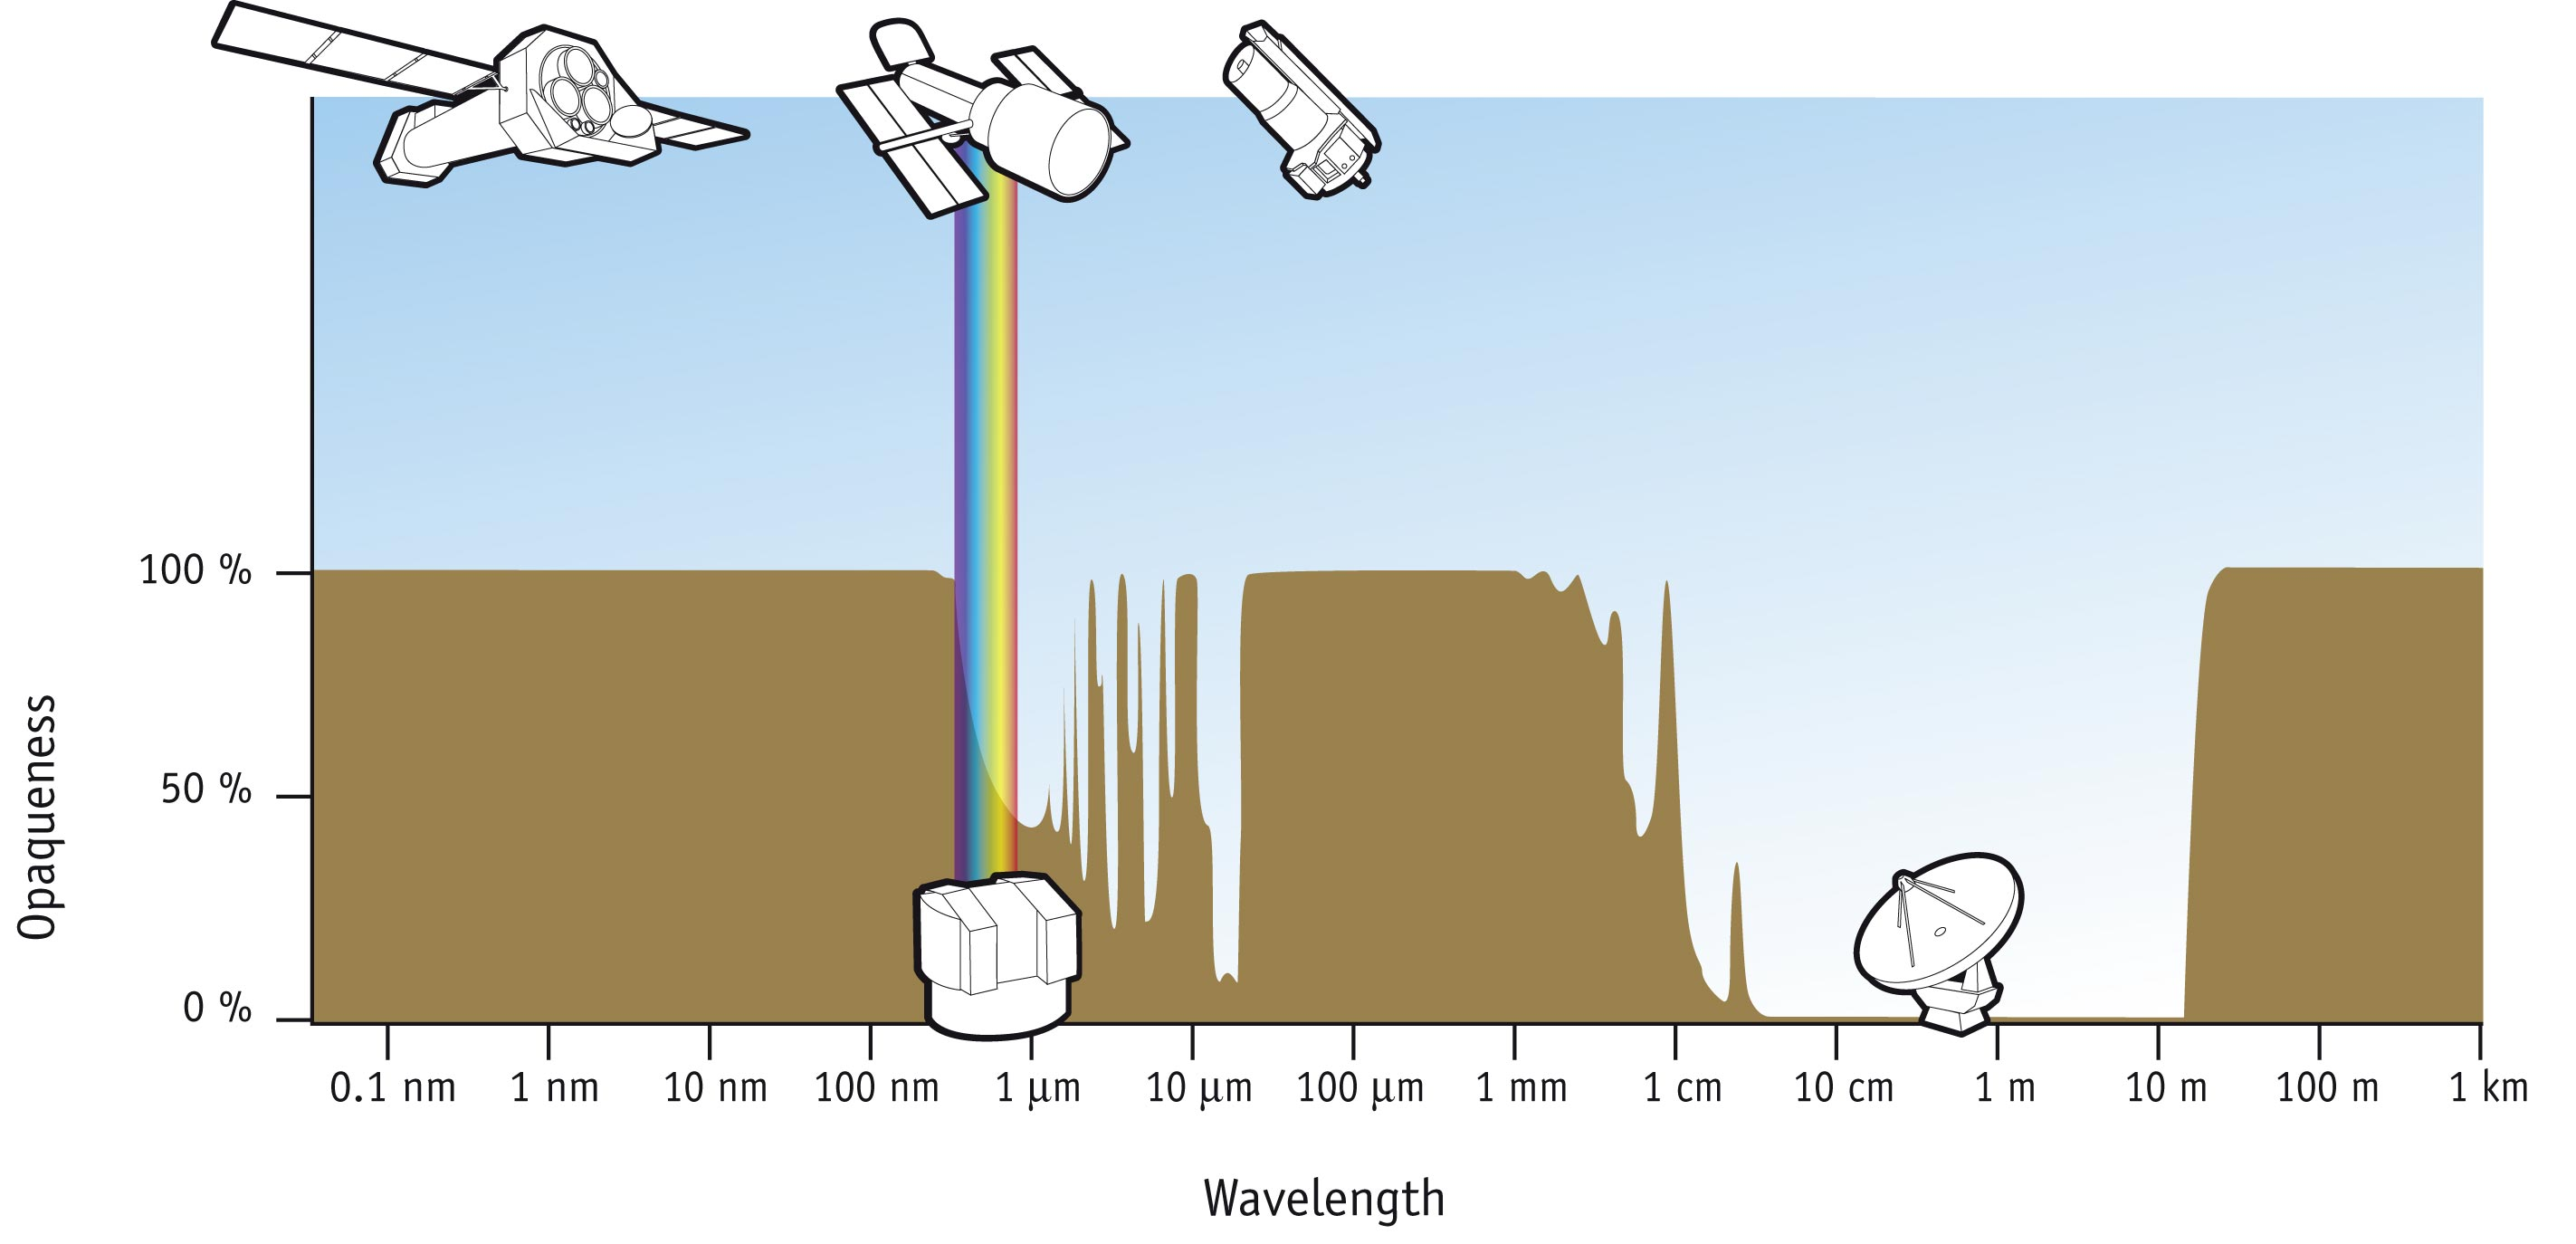
\includegraphics[width=\columnwidth]
		{fig/AtmosphericOpaquenessVsWavelength.png}
	\caption[Atmospheric opaqueness versus wavelength.]
	{
		Atmospheric opaqueness as a function of wavelength. Earth's
		atmosphere is opaque to most electromagnetic radiation,
		except for the visible window, which reaches from the
		near-infrared to the near (soft) ultraviolet radiation.
		There is also a radio window for electromagnetic radiation
		with wavelengths between 1~mm and several tens of meters,
		and it is not totally opaque for radiation above the $1/10$
		of a millimetre. The main responsible for atmospheric
		absorption of sub-mm radiation is water vapour, and dry
		regions such as those in the South Pole or in the Atacama
		Desert can be used for observations in the sub-mm range.
		This image was created for NASA by STScI under Contract
		NAS5-26555 and for ESA by the Hubble European Space Agency
		Information Centre, and is in the public domain.
	}
	\label{fig:fig_AtmosphericOpaquenessVsWavelength}
\end{figure}

	 Then came the new windows opened when the space career
	started, allowing humankind, for the first time, to have
	observatories outside of the atmosphere, which is opaque for
	radiation other than radio and visible light ---see
	figure~\ref{fig:fig_AtmosphericOpaquenessVsWavelength}---. We
	were rewarded with the discovery of strong X-ray sources marking
	active galaxy nuclei, supernovae, and the incredibly bright and
	distant Gamma-Ray Bursts. By being free of the atmosphere, the
	Hubble Space Telescope has provided us with the deepest view of
	our Universe, thanks to the repeated, accumulated exposure of
	the Ultra Deep Field~\cite{2006AJ....132.1729B}.
	
	 Of course, our current observatories, both ground-based and
	space-borne, have only been possible after Charge Couple
	Devices (CCDs) started to replace photographic plates. The
	sensibility of CCDs (measured as their quantum efficiency, or
	percentage of times a photon incidence produces a measurable
	change in the sensing element) is much superior to that of
	photographic plates, allowing the detection of fainter
	objects. Besides, several other capabilities, specially direct
	electronic output and linearity in their response, make them
	much more desirable than film for scientific, and particularly
	astronomical purposes.

% section astronomy_technical_developments (end)

\section{Astronomy data today} % (fold)
\label{sec:astronomy_today}

	%	\begin{figure}[tbp]
	%		\centering
	%			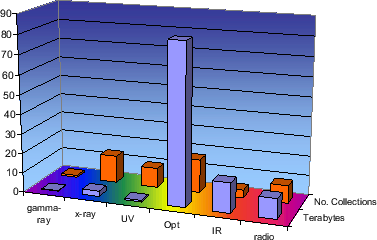
\includegraphics[width=\columnwidth]{fig/img7.png}
	%		\caption{caption}
	%		\label{fig:fig_img7}
	%	\end{figure}

	Contemporary astronomy is built around the idea of digitised
	observations. Everything is quantised, digitised, and processed
	using digital computers, something made easier by the digital
	nature of CCDs.
	
	 This digital nature makes it more natural to mix datasets from
	different observatories, giving birth to what is called
	multiwavelength astronomy. By combining the light received from
	as many instruments as possible, we can learn an increasing
	number of properties of distant objects. For instance, we can
	try to fit spectral models to the actually recorded spectrum,
	being that fitting more reliable when considering the most
	bands.
	
	 Building that multiwavelength picture is, nevertheless, not
	trivial. Astronomers need to perform their own observations
	of the objects of their interest with many different
	observatories and instruments, something very costly in terms
	of both time (observation proposals have to be written, and if
	approved then the actual observation has to be performed,
	processed, and analysed) and effort (spent in learning the
	different packages needed to reduce astronomical data from
	different observatories); or instead, astronomers can rely on
	observations previously performed by other astronomers, and
	stored in the archive of observatories of their interest.
	
	 In any case, very few observatories have archives, and
	those which have them provide datasets with very different
	science requirements. Some observatories provide raw data,
	which have to be combined with calibration data for the
	astronomer to perform the data reduction, while others provide
	already reduced data products with very little information on
	how that reduction was performed, which were the observing
	conditions, and so on. Each different archive is accessed
	through its own access portal, has different access policies,
	different data browsing mechanisms, and data are finally
	delivered in different formats. And there is the additional
	issue of finding out which archives exist which carry data of
	our interest.
	
	 An interesting exception to the lack of archives are
	space-borne observatories. These facilities are so expensive,
	essentially due to the launching costs,\invisiblenote{but also
	to the research and development invested into the satellite,}
	that collected data have to be made available to the community
	after typically one year of proprietary period in order to
	maximise the scientific return from their observations. The
	cost of the archive is a small fraction of the operational cost
	for the mission, and all space satellites provide some sort of
	access to their archives. The kind of data products provided by
	each mission, however, is not standardised, either.

	\invisiblenote{
	 In the late seventies, the use of digitised imaging, and the
	need of computer-intensive Fast Fourier Transforms for imaging
	in radio interferometry made several institutions create, in
	the late seventies, a common Flexible Image Transport System,
	the FITS file format. That data format was presented to the
	community in 1981~\cite{1981A&AS...44..363W}, and solved part
	of the problem of image (and spectral, and tabular data)
	transport, but the flexibility of the system made FITS files
	not fully compatible between different software packages.
	}
	
	%	\footnote{To be fair, astronomy has had since the 70's a common
	%	data format, the Flexible Image Transport System (FITS), to
	%	which most archives and instruments adhere. However, the
	%	complexity of many astronomical observations allow for very
	%	different layouts of the data, and FITS headers are not always
	%	easy to read for a machine in order to interpret available
	%	data.}.

	 A third source of data for the astronomer are large sky surveys,
	which have started to take place in the last few years, in which
	data are collected by dedicated wide-field telescopes, with
	reduction pipelines working for several spectral bands. The
	pipelines perform digital processing on the images, and
	determinate tens or hundreds of properties for selected objects.
	Such is the case of recent surveys, such as the Sloan Digital
	Sky Survey (SDSS)~\cite{1995wfsd.conf....3G,
	2000AJ....120.1579Y}, such as the Two Micron All Sky Survey
	(2MASS)~\cite{2006AJ....131.1163S}, but also for the digitised
	version of the Second Palomar Observatory Sky Survey (POSS-II,
	D-POSS), or even the older, National Geographic Society-Palomar
	Observatory Sky Survey (NGS-POSSdigitised).

	% Remember, the Digitised POSS-I conforms
	% the Digitised Sky Survey,
	% base of the Microsoft World Wide Telescope,
	% y de Google Sky.

	 Not all surveys are optical, and there are radio surveys such
	as the the FIRST~\cite{1994ASPC...61..165B} and
	NVSS~\cite{1993BAAS...25.1389C} surveys, performed with the
	Very Large Array radio interferometer (VLA), or the
	ALFALFA~\cite{2008arXiv0806.1670H, 2005AJ....130.2598G}, being
	performed with the Arecibo radio telescope.
	
%	The problem the astronomer faces today is twofold:
%	
%	\begin{itemize}
%		\item how to retrieve everything that is available from all
%        the different archives, in order to know whether he needs to
%        apply for observation time or not; and
%		
%		\item how to access all information at the same time in
%        order to derive statistical properties.
%	\end{itemize} 
%	
%	This last point is of the utmost importance for extragalactic
%    astronomy, given than most galactic processes have time scales
%    of giga-years, and in that case we are looking essentially at a
%    snapshot of the universe. If we want to derive properties, we
%    need to compile statistics for objects of the same kind, but for
%    those statistics to be meaningful we need to use very large
%    samples. And for those large samples to be built we need to
%    access a large amount of archives whose organisation (as of now)
%    is completely different, and whose access interfaces were
%    thought for the individual astronomer, not for direct machine
%    interrogation.

% section astronomy_today (end)

\section{Astronomical archives: benefits and problems} % (fold)
\label{sec:astronomical_archives}

	As pointed in the section before, self-performed observations
	are but one of the ways for astronomers to collect data
	relevant to their research, while data archives, be them
	originated from the systematic storage of observational data
	from each telescope and instrument, from broad sky surveys, or
	from space-borne missions, conform nowadays the main resource
	of astronomical data.
	
	 Archives provide several benefits for astronomers:

	\begin{description}
		\item[Efficiency in resource usage] If the observation an
		astronomer wishes to perform has already been made, there
		is no need to go through the full process of writing
		observation proposals or to wait for the allocated time.
		The data can be downloaded by many different users, serving
		many different purposes, some perhaps never considered at
		the time of the observation.
		
		\item[Time domain exploration] Some astronomical objects
		have properties varying in time. Comparing observations
		taken in different moments allows to study periodic
		phenomena (variable stars, asteroid rotation, pulsars, et
		cetera), or transient phenomena (novae and supernovae,
		Gamma-Ray Bursts, et cetera)
		
		\item[Statistical inference] Most astronomical processes %
		(specially those regarding extra-galactic astronomy) have
		time scales much larger than our civilisation life-span,
		and our only way to explore them is to take into account as
		many objects of the same type as possible. This includes
		defining object types, something which can be simplified by
		data mining techniques, which in turn require large
		datasets to explore.
		
		\item[Non-exclusive access] Public archives allow
		astronomers from countries with limited research resources
		to access high-quality data, and produce top-level science.
	\end{description}

	However, in their current incarnation, archives pose several 
	problems:

	\begin{description}
		\item[Ever increasing datasets] There is no way to know when
		a particular observation will be useful, so all observations
		must be stored, and together with them all the ancillary
		data (weather conditions, seeing, opacity, telescope
		orientation, instrumental calibration observations, et
		cetera) needed to reduce the raw observation data in order
		to get scientific data products. That means every year
		archives have to manage more and more data. An example can
		be seen in figure~\ref{fig:fig_ESODataHoldings}.
		
		 \item[Ever increasing dataset size] Telescopes are built
		with 25 to 50 years life-spans, but instruments are changed,
		improved, and added, so that the same telescope can provide
		more and more resolution and sensitivity over the years, as
		CCDs tend to follow Moore's Law~\cite{1965E......38.....M},
		and double every two years ---see
		figure~\ref{fig:fig_CCDresolutionIncrease}---. That makes
		each dataset to be archived larger for each new facility or
		instrument.
		
		 \item[Ever improving data reduction techniques] The actual
		data being collected are in the form of voltages, or
		detection counts, that have to be converted in physical
		magnitudes such as temperature, emitted energy, mass, et
		cetera, which can be derived thanks to the knowledge of all
		the physical processes affecting the measurement, but also
		to a very careful measurement of observational effects. When
		the technical knowledge of those effects improves, many
		archives provide a new version of the derived data,
		contributing both to the data increase, but also to the need
		to document how each version has been obtained.
		
		 \item[Non-uniform, non-centralised access] Nowadays, most
		instrumental archives are accessible via internet, but each
		different telescope ---or even each different instrument---
		has a different web portal, with different query parameters,
		which are difficult to access in an automated way. Besides,
		there is no way for an astronomer ---much less so for a
		software system--- to learn when a particular archive, or
		data set within that archive, has been released, as many
		observations are held for a certain \emph{proprietary
		period} during which the original observer has exclusive
		access to it.
	\end{description}

	\begin{figure}[btp]
		\centering
		%\includegraphics[width=0.8\columnwidth]
		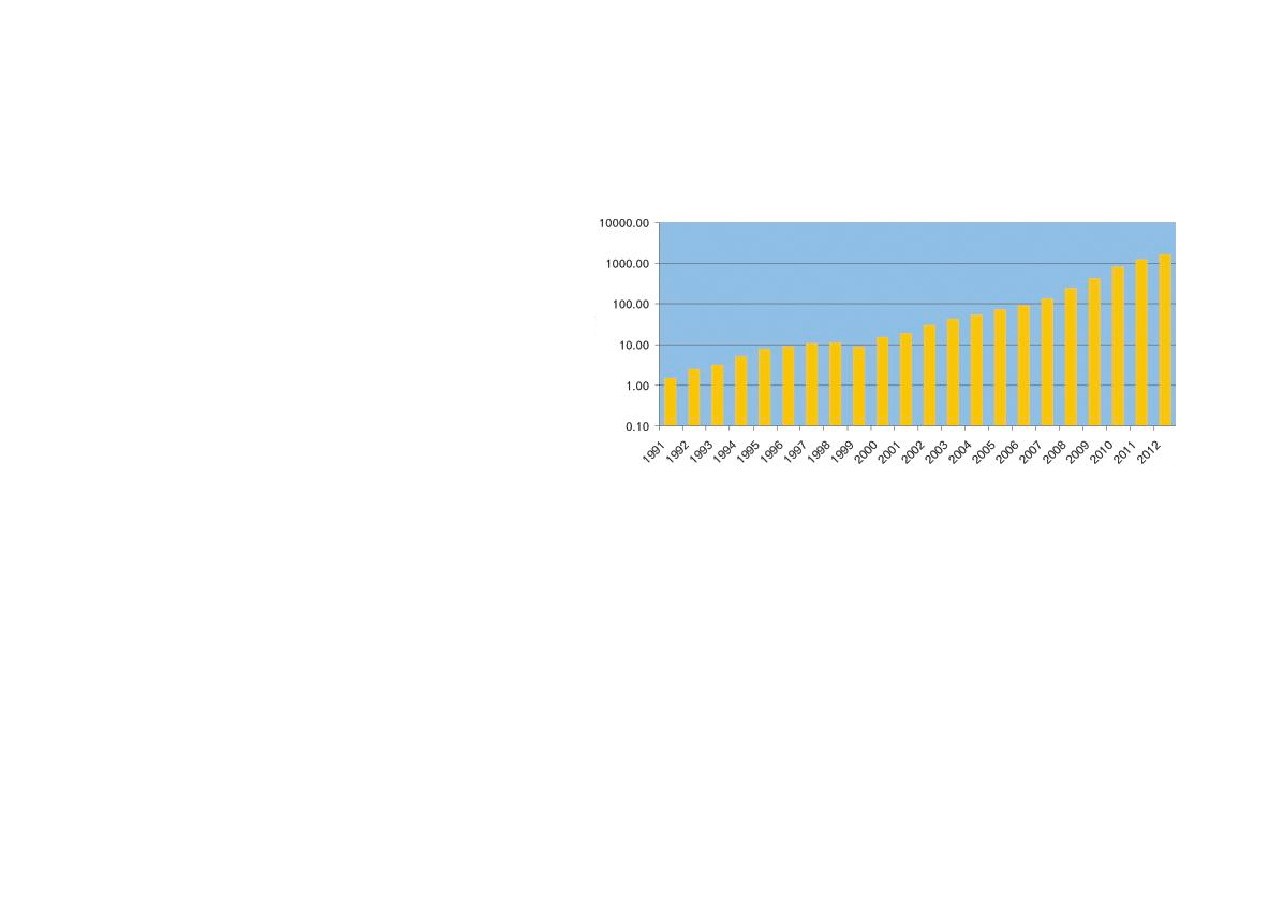
\includegraphics[scale=1]
				{fig/ESODataHoldings.pdf}
		\caption[Evolution of the
		         ESO data holdings]
		{
			Evolution of the amount of data stored in the ESO
			archive since 1991 to 2003 (in Terabytes in logarithmic
			scale), together with predictions till 2012.
			Reproduced from~\cite{ESO:2003la}.
		}
		\label{fig:fig_ESODataHoldings}
	\end{figure}

	\begin{figure}[btp]
		\centering
		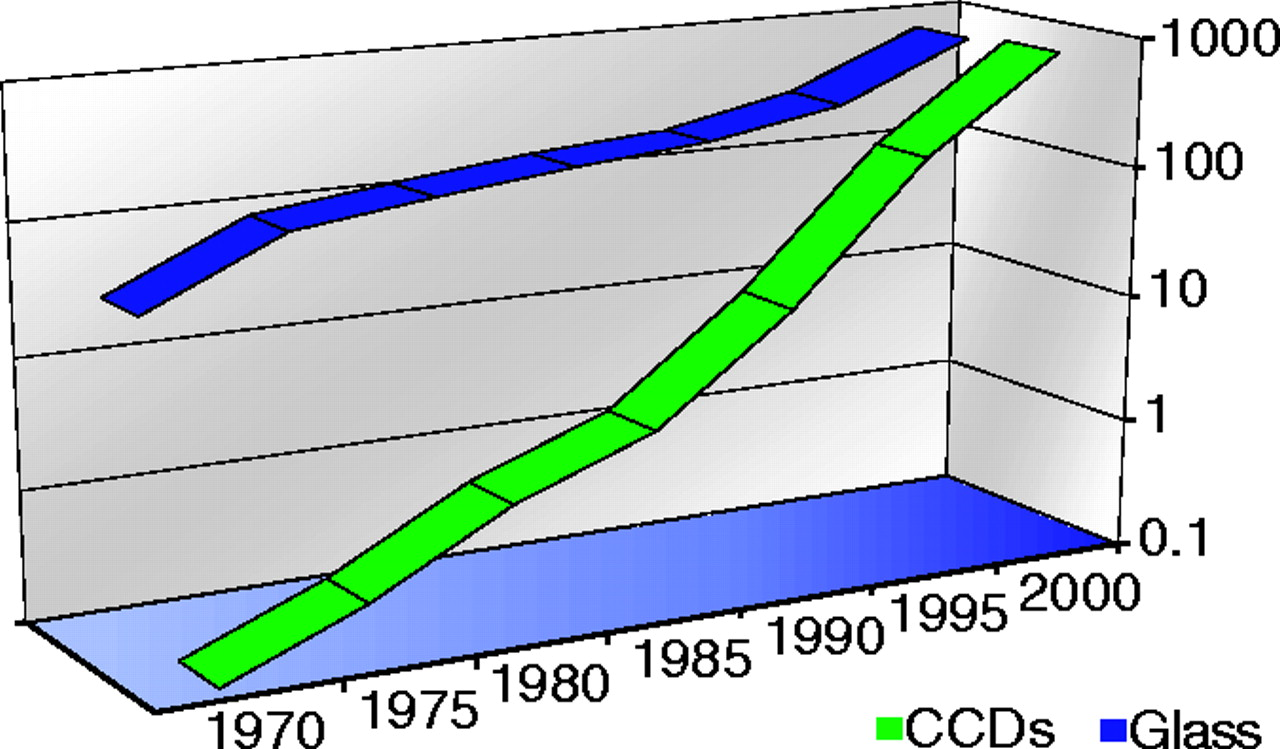
\includegraphics[width=0.8\columnwidth]
		     {fig/CCDresolutionIncrease.jpg}
		\caption[Evolution of telescope areas and CCD pixel resolution]
		{
			Telescope collecting surface area (labelled Glass) and
			CCD pixel resolution in logarithmic scale versus linear
			time since 1970 (arbitrary units). It can be seen that
			CCDs, governed by \glossaryentry{Moore's Law}, have a
			much steeper increase rate, doubling roughly every 2
			years, whereas telescope area doubles every 25 years.
			Reproduced from~\cite{2001Sci...293.2037S}.
		}
		\label{fig:fig_CCDresolutionIncrease}
	\end{figure}

	 Thus, astronomers in the era of archives face the following
	problems:

	\begin{itemize}
		\item finding out and retrieving already available data from
		existing archives, remaining aware of additional datasets
		which might be released at any time;
		
		 \item combining datasets from different archives in a
		sensible way;
		
		 \item managing huge datasets simultaneously in order to
		derive statistical properties;
		
		 \item performing analysis of large datasets on a
		distributed system; this problem is compounded by the
		bottleneck of network bandwidth, which not increasing at the
		same rate as the astronomical data set size.
	\end{itemize}

	A suitable solution for those issues, then, should provide:

	\begin{itemize}
		\item Mechanisms for finding each and every data repository
		available in each moment must exist.
		
		 \item Complete descriptions of each data repository, so
		that those not containing data of interest for the
		astronomer ---as specified by several selection criteria,
		such as wavelength or resolution--- can be filtered out.
		
		 \item Unified data description and format, so that data
		coming from heterogeneous sources can be easily combined,
		and operated with.
		
		 \item Minimum data transfer between users of archived data
		and the data; data processing must be moved preferentially
		to the server, and only processed data should be sent back
		to the astronomer.
	\end{itemize}

	Such a system would provide each astronomer in the world with a
	virtual observing facility able to picture the sky in all the
	wavelengths at the same time, without the need for the
	astronomer to manually discover each of the datasets which will
	conform that picture, or to perform conversions on data coming
	from different instruments. That system exists, and is called
	the Virtual Observatory.
	
	 Discussions on the Virtual Observatory concept were started
	with the \emph{Virtual Observatories of the
	future}~\cite{2001ASPC..225.....B}
	and \emph{Mining the sky}~\cite{2001misk.conf..674G}
	conferences, held
	in 2000 at Caltech and Garching bei Müenchen, respectively.
 	The north american
	National Virtual Observatory project started in 2001 with a 
	10 million dollar funding, and 17 centres involved. Finally,
	Jim Gray and Alex Szalay summarised and generalised the concept
	in their 2001 article \emph{The World-Wide
	Telescope}~\cite{2001Sci...293.2037S} in \emph{Science}, and the
	community
	started prototyping the system in 2002.
	
	 However, many different \emph{virtual observatories} can be
	built following the previous definition.
	In order to have a single
	Virtual Observatory where all datasets and tools are
	interoperable, standards need to be set and adhered to. Thus a
	standards sanctioning body is needed, and that is the role of
	the International Virtual Observatory Alliance (IVOA).
	
	 The VO is still in development, but nearing what is called the
	\emph{operations stage}, where astronomers are regularly using
	VO tools for their research. However, in this thesis will see
	that there are several problems with the current incarnation of
	the VO, particularly in the scope of radio astronomy, and
	multidimensional data access.
	
	In Spain, the national VO initiative is the Spanish Virtual
	Observatory (SVO), which joined the IVOA in 2004, and which is
	focused in promoting science with the VO in Spanish astronomy,
	and in providing specific tools for performing that science.
	
	We wish to emphasise that this is the first technical thesis
	developed within the SVO framework.

% section astronomical_archives (end)

\section{Thesis aim} % (fold)
\label{sec:thesis_aim}
	
	This thesis is devoted to the study of:

	\begin{description}
	
		\item [The VO infrastructure] Which are the components of
		the VO, and which are the interfaces to them, with special
		emphasis on missing or underdeveloped blocks for radio
		astronomical data. This is the scope of
		chapter~\ref{intro_vo} of Part~\ref{prt:intro_vo}.
	
		 \item[Modelling radio astronomical data] For radio
		astronomical data to be properly described within the VO
		data models are needed. Part~\ref{partRadioDataModelling} is
		devoted to the RADAMS, the data model developed for radio
		astronomical observations.
	
		 \item [Bringing legacy tools to the VO] As there are many
		man-years of experience invested in many already existing
		astronomical tools, we will study how to incorporate those
		tools into the VO ecosystem. We have developed a Modular VO
		Interface for Radioastronomy (MOVOIR) which provides both a
		GUI for accessing the VO, and tools for adapting legacy
		tools to use VO protocols. Part~\ref{prt:legacyTools} is
		devoted to it.
	
		 \item [Applied work] We have used the RADAMS data model as
		the basis for the astronomical archives of the IRAM~30m and
		DSS-63~70m radio telescopes, and the MOVOIR as the basis for
		bringing the \massa{} and \madcuba{} legacy
		applications into the VO. We show our results in
		Part~\ref{prt:thesis_applications} is devoted to the
		archives which have been built using the RADAMS.
	
	
	\end{description}

	As a result of this study, complete VO-compliant radio astronomy
	model has been created, two astronomical archives have been
	implemented, and a software tool has been developed for allowing
	legacy radio astronomical tools access the VO.

% section thesis_aim (end)


\section{Thesis context} % (fold)
\label{sec:thesis_context}

	This thesis work has been developed and written
	\invisiblenote{not
	within a computer science research group, but} within an
	astrophysical research project
	(AMIGA\urlnote{http://amiga.iaa.csic.es/}, Analysis of the
	interstellar Medium of Isolated GAlaxies) whose objective is
	studying a sample of isolated galaxies, with more than 1000
	members. A special emphasis is given on radio observations in
	the centimetre, millimetre, and sub-millimetre wavelength ranges
	because the (sub)mm spectral band delivers fundamental
	information to learn about physicochemical processes in the
	interstellar medium (ISM). It is relevant to note that astronomy
	in the (sub)mm range is suffering a strong technological
	advance, with new astronomical facilities, such as the
	Sub-Millimetre Array\urlnote{http://sma1.sma.hawaii.edu/} (SMA),
	and the well-advanced construction of the Atacama Large
	Millimetre Array\urlnote{http://almaobservatory.org/} (ALMA).
	
	 As public data access in the radio wavelength is limited, we
	had resolved to contribute in the building of radio data
	archives, working together with the IRAM to provide an archive
	for the IRAM 30m antenna. In parallel, we also undertook the
	development of the scientific archive for spectroscopic
	observations of the DSS-63 70m antenna at Robledo de Chavela,
	part of NASA's Deeps Space Network.
	
	\newcommand{\massaurl}[0]
	{http://damir.iem.csic.es/mediawiki-1.12.0/index.php/Portada}
	 Since our group does intensive analysis of 3D data at all
	wavelengths (in fact the current trend in spectroscopy), we
	also decided to collaborate in bringing existing software
	packages to solve the mentioned tasks, in order to make our
	research work more efficient. We have collaborated with Jesús
	Martín-Pintado's group at the Molecular and Infrared
	Astrophysics Department (DAMIR) of the Institute of Matter
	Structure, developers of the MASSA (MAdrid Single Spectrum
	Analysis) and \madcuba{} (MADrid CUBe Analysis)
	tools\footnote{Project wiki: \url{\massaurl}} for the Heterodyne
	Instrument for the Far
	Infrared\urlnote{http://www.sron.nl/divisions/lea/hifi/} (HIFI)
	of the soon to be launched Herschel
	spacecraft\urlnote{http://herschel.esac.esa.int/}, in order to
	make both tools compatible with the VO.
	
	 All the problems we need to solve are very similar to those of
	the astronomical community at large (save the emphasis in the
	radio band), namely:

	\begin{itemize}
		\item easy-to-use data look-up tools, in order to get
		multi-wavelength data for every object, to be retrieved from
		online archives;
		
		\item data combination tools, taking into account different
		data formats, coordinate systems, file metadata;
		
		\item physical parameter extraction tools: each different
		parameter must include different physics, and needs its own
		interface.
	\end{itemize}

	The community had already started to provide an
	information-technology-based solution: the Virtual Observatory.
	All the work performed for this thesis has been built within
	that framework, and in collaboration with the Spanish Virtual
	Observatory initiative.
	
% section thesis_context (end)

 % \todo{end introduction}
	%Rule for 71 characters
%2345678901234567890123456789012345678901234567890123456789012345678901

\chapter{The Virtual Observatory} % (fold)
\label{intro_vo}

% \lourdes{Coherencia: buscar ... y quitar o cambiar por et cetera.}
% \lourdes{Coherencia: cambiar et cetera por etcetera.}

% One of the most important achievements of modern astronomy is the %
% digitisation of many relevant datasets, either by scanning old
% photographic plates, or by directly using CCDs or other electronic
% and
% computerised means for data collection. Many archives are available
% which provide astronomers with lots of information without having to
% point themselves a telescope to the sky.
% 
% However, the use of archives brings its new share of problems:
% 
% \begin{description}
% 	\item[Growing list of archives] With new instruments bringing
% 	their own archives, each year a score of new archives joins the
% 	wealth of information available to astronomers. Astronomers,
% 	or software tools, must be notified of the release of
% 	a new archives, and in many cases software would need upgrading
% 	in order to operate with new archives.
% 	
% 	\item[Archive heterogeneity] As each archive is developed by the
% 	team responsible for the corresponding instrument development,
% 	dataset storage, query, and retrieval are created differently for
% 	each instrument or telescope, leading to a strong heterogeneity
% 	both between data products and query methods. Different query
% 	codes have to be written in order to deal with 
% 	
% 	\item[Terabyte-class archives] Archives are growing exponentially
% 	larger, because even when old archives provide a linear storage
% 	rate, new archives provide much larger data rates per day, as
% 	sensitivity and pixel resolutions increase as per Moore's
% 	Law.
% \end{description}

\invisiblenote{
	vir•tu•al |ˈvər CH oōəl| 
	adjective 
	almost or nearly as described, but not completely or according to strict definition : 
	the virtual absence of border controls. 
	• Computing not physically existing as such but made by software to appear to do 
	so : a virtual computer. See also VIRTUAL REALITY . 
	• Optics relating to the points at which rays would meet if produced backward. 
	• Physics denoting particles or interactions with extremely short lifetimes and 
	(owing to the uncertainty principle) indefinitely great energies, postulated as 
	intermediates in some processes.

ob•serv•a•to•ry |əbˈzərvəˌtôrē| 
noun ( pl. -ries) 
a room or building housing an astronomical telescope or 
other scientific equipment for the study of natural 
phenomena. 
• a position or building affording an extensive view. 
}

\attributedquote{
	\dictionarydef
	{virtual}
	{adjective}
	{
		\begin{itemize}
			\item almost or nearly as described, but not completely
			or according to strict definition: 
			\emph{the virtual absence of border controls}.
			
			\item \textsf{Computing} not physically existing as
			such but made by software to appear to do 
			so: \emph{a virtual computer}.
		\end{itemize}
	}
	\dictionarydef
	{observatory}
	{noun}
	{
		\begin{itemize}
			\item a room or building housing an astronomical
			telescope or  other scientific equipment for the study
			of natural phenomena.
			
			\item a position or building affording an extensive
			view. 
		\end{itemize}
	}
}
{The New Oxford American Dictionary, \emph{2nd Edition}}


	
% section the_vo_and_archival_issues (fold)
\section[The VO: solving astronomical archival issues]
[The VO: solving astronomical archival issues]
{The Virtual Observatory: solving astronomical archival issues}
\label{sec:the_vo_and_archival_issues}
	
	In the previous chapter the current status of multi-wavelength,
	archive based astronomy was laid as well as the problems
	arising when dealing with the increasing number of data
	archives available to the astronomical community, and with the
	increasing sizes for each data unit. Additionally, these data
	units must be combined in order to obtain a multiwavelength
	view of our universe.
	
	 As the archives are already distributed across the world, the
	solution must be network-enabled, and must be as modular as
	possible, so that different data providers and astronomical
	tool developers can work independently, and rely on common
	interfaces. A Service Oriented Architecture (SOA), where data
	providers create web-services, and tool developers use
	web-services interfaces to query them fits that description,
	and allows reuse of already existing and deployed technology.
	
	 It must be noted that astronomical data reduction for large
	instruments is a highly specialised task, and that data
	reduction techniques are improved when knowledge about the
	underlying processes (astrophysical and observational)
	improves. This specialisation, and the long term variability of
	reduction techniques, makes unfeasible the centralisation of
	astrophysical archives.
	
	 In any case, those services must be oriented to astrophysics,
	and responses must include metadata describing the
	peculiarities of each data set. \invisiblenote{The choice of
	SOA makes XML the perfect language for holding the metadata for
	astronomical data sets.} Lastly, in order for applications to
	find out both existing and new services and data sets, a common
	service registry is needed for VO applications to find out
	suitable services and data sets.
	
	 Jim Gray and Alexander Szalay, in ``The World-Wide
	Telescope''~\cite{2001Sci...293.2037S}, were among the first to
	outline such a system, which is called the Virtual Observatory
	(VO). In that paper, they analysed the already mentioned
	exponential trends of instrumental data output and archived
	data holdings increase, and noticed the not equally growing
	gain in astrophysical insight as an unmistakable sign that
	astronomers were not being able to cope with the new
	data-driven situation, and needed new tools to get the most of
	the extremely large datasets now available to them.
	
	 An example of a widely used, very large astronomical dataset
	is the already mentioned SDSS. In its latest release (DR7), the
	SDSS consists of more than 15~TB of image data, plus more than
	25~TB of ancillary data, and 18~TB of catalogue data. There is
	not enough bandwidth at the SDSS or at the different research
	institutions to transfer all the data to all researches which
	would like to use the SDSS. And in the future, surveying
	telescope such as the Large Synoptic Surveying Telescope (LSST)
	will produce and process around 7~TB of raw data per night.
	
	 Exploiting this ever-increasing amount of data is only
	feasible by scientific-case guided data selection, together
	with automated data mining techniques. But for that to be
	performed in a fully automated way, data archives and data
	analysis tools must become interoperable.

	% \lourdes{Reordenar conforme capítulo.}

	For achieving the interoperability we will need, as stated by
	F.~Genova in her ``Interoperability''
	article~\cite{2002ASPC..281...41G}:
	
	\begin{itemize}
		\item common data formats;
		
		 \item common data access protocols; and
		
		 \item common data models for the same type of
		observations, as independent as possible of the generation
		of the dataset, so that data from very different
		observatories and instruments can be combined.
	\end{itemize}
	
	 In addition, as VO services are distributed across the globe,
	and can be deployed anywhere, anytime, one or several services
	registries are needed, so that users can find and discover new
	services.
	
	 But for those common formats, protocols and data model to
	become truly compatible an standardisation body is needed. In
	the VO, that body is the International Virtual Observatory
	Alliance.
	
	 In the next sections we will see how the VO achieves archive
	interoperability, which mechanisms provides for minimising
	local data processing as much as possible, and what is the high
	level organisation of the IVOA.
% section the_vo_and_archival_issues (end)


\section{VO architecture and philosophy} % (fold)
\label{sec:vo_architecture}

	In Gray and Szalay's paper~\cite{2001Sci...293.2037S}, the
	stated philosophy for the VO is that of an
	e-infrastructure\footnote{The \emph{e} in e-infrastructure does
	not stand for \emph{electronic}, but for \emph{enhanced}, as in
	\emph{e-Science}, or \emph{enhanced science}. The enhancement
	is produced by means of the massive use of networked resources,
	such as data grids, computation grids, distributed storage, et
	cetera, which conform the \emph{e-infrastructure}.} which makes
	all astronomical data in the world available for astronomers as
	if they were in their own desktop, without the limitations of
	desktop computing.
	
	 For many large datasets the user should not deal with the data
	directly, as the data transport time for many modern datasets
	is not negligible, and the data producer's infrastructure can
	be better suited for remote processing. In time, remote
	processing has to become commonplace, as it will become the
	only solution to let users ask questions to datasets much
	larger than typical workstation can manipulate, avoiding
	network bottlenecks at the same time.
	
	 In any case, sufficient metadata must be provided so that
	astronomers do not need to download data to see if they can be
	useful or interesting, and perform instead a suitable selection
	of datasets based on metadata. In particular, data quality
	assessment through metadata inspection and evaluation allows
	astronomers not to retrieve, for instance, low resolution
	datasets if they need precise astrometric measurements, while
	other astronomers interested on obtaining upper limits of an
	object's emissions might find them useful.

%	\lourdes{redactar el párrafo anterior para que no indique que
%	se usen datos faulty, sino quizá upper limits o similares o not
%	fully calibrated}

	How is that vision actually implemented?
	Figure~\ref{fig:fig_VOArch} portraits a simplified,
	all-encompassing vision of the Virtual Observatory. In that
	figure we see the Virtual Observatory from the lowest level
	supporting implementation (network cabling, routers, storage
	media, et cetera; what is usually known as \emph{the iron}), to
	base internet protocols, and grid computing middleware, to VO
	services and protocols implemented on top of that
	infrastructure, and applications using both services and
	protocols to present the user with a unified interface.

\newcommand{\voarchitecturenoteurl}[0]
{http://www.ivoa.net/Documents/Notes/IVOArch/IVOArch-20040615.html}
	\begin{figure}[tbp]
		\centering
			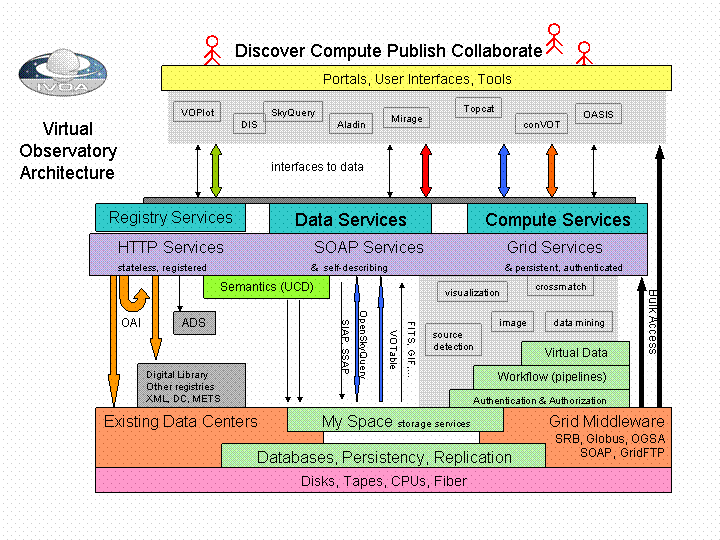
\includegraphics[width=\columnwidth]
			{fig/VO_Architecture.png}
		\caption[Virtual Observatory architectural overview]
		{
			Architecture of the Virtual Observatory, seen from the
			low level implementation (bottom) to the user (top).
			Users perform high-level activities, such as
			computations, data discovery, data mining, and even
			publishing into the VO by means of applications,
			scripting tools, or web portals. Applications
			communicate with the VO by means of IVOA approved
			protocols to access the service Registry, Data Services
			to retrieve astronomical images, spectra or, in the
			near future, complex table access to astronomical
			databases. Computing Services are needed for those
			computations which are costly to perform locally due to
			bandwidth or processor requirements. Registries
			communicate with each other via the Open Archive
			Initiative (OAI) harvesting protocols, to ensure that
			registry changes propagate from each registry to the
			rest. Registries are queried through SOAP-based
			protocols, to ensure compatibility with other OAI
			registries, while the remaining VO protocols use simple
			HTTP GET (REST-ful) interfaces. From the IVOA Virtual
			Observatory Architecture Overview diagram,
			\url{\voarchitecturenoteurl}.
			% \todoinline{Recreate simplified diagram.}
		}
		\label{fig:fig_VOArch}
	\end{figure}

%	Figure~\ref{}, on the other hand, provides a mind map of the
%	Virtual Observatory concepts. The

	 It is legitimate to ask how far is the Virtual Observatory
	today from being completely transparent to the user. The answer
	to that is that there are several factors which make the
	Virtual Observatory still a separate environment for
	astronomical research:

	\begin{itemize}
		\item VO applications and portal are still unknown to many
		astronomical users, including some data providers. The
		different VO groups are making an effort in the
		dissemination of the VO concept, both for astronomical
		users and data providers. Many different workshops and
		schools are being promoted in order to reach users and
		providers.
		
		 \item Many interesting datasets are still not available
		via the VO. The NVO and the Euro-VO projects, are
		developing tools to make data publishing easier for small
		research groups. However, they demand a high level of
		computing expertise in the domain of networking, web
		services technologies, XML, and of the inner workings of
		the VO. Besides, a commitment to maintain the archive
		operational in the long term means the research group has
		to keep storage and network resources with a high level of
		availability. This makes it difficult for those small
		groups to become data publishers if they do not deploy a
		complete archive.
		
		 \item Many different useful tools for astronomers predate
		the Internet era, with many legacy tools unable to access
		Virtual Observatory datasets.
	\end{itemize}

%	This thesis tries to address these three concerns, in the
%	framework of radio astronomy. In this thesis:
%
%	\begin{itemize}
%		\item We present the VO both from the astronomical and
%		computer science sides, so that more developers can
%		contribute to the VO, and more astronomers are made aware
%		of its posibilities.
%		
%		 \item We provide a framework for radio astronomical
%		observation characterisation and data publishing, which has
%		actually been used for the development of the IRAM~30m and
%		Robledo's DSS-63 archive.
%		
%		 \item We follow different strategies for making legacy
%		astronomical applications aware of the VO, and able to use
%		VO datasets.
%	\end{itemize}

% 	\subsection{The VO protocol stack} % (fold)
% 	\label{sub:the_vo_protocol_stack}
% 
% 	\setlength{\epigraphwidth}{0.66\columnwidth}
% 
% 	\epigraph{
% 		Any problem in computer science can be solved with another
% 		level of indirection... but that will usually create another
% 		problem.
% 	}
% 	{\textsc{David Wheeler}, as quoted by \textsc{Butler Lampson}}
% 	
% 		The architecture of the VO can be seen in a simplified way by
% 		means of the OSI diagram. Figure~\ref{} shows the typical
% 		depiction of a network protocol stack, where different
% 		machines communicate between them conceptually at the same
% 		level, while the actual communication is from the upper part
% 		of the stack to the lower part, with results from the lower
% 		parts to the upper parts.
% 		
% 		 In that view, each layer calls services in the lower layer,
% 		so that higher-level capabilities (rendering of web pages, for
% 		instance) rely on a protocol layer (HTTP), which relies on a
% 		transport protocol (TCP), relying on a network routing
% 		protocol (IP), which relies on data link and physical
% 		technologies, such as wired or wireless networking over
% 		Ethernet, LocalTalk, Token Ring, or any other networking
% 		settings.
% 		
% 		 In the case of the VO, interchanges happen at the Application
% 		and Presentation layers, as all of IVOA protocols are based on
% 		top of HTTP and HTTPS (some of them can use other protocols,
% 		but HTTP/S is a requirement)
% 	
% 	% subsection the_vo_protocol_stack (end)

% section vo_architecture (end)

% \todoblock{
% 	When talking about VO architecture, present the VO from the 
% 	point of view of:
% 
% 	\begin{itemize}
% 		\item the user [done]
% 		\item the VO application (developer) [done]
% 		\item the VO service (developer)
% 		\item the data centre/scientist wishing to publish on VO
% 		\item the infrastructure provider
% 	\end{itemize}
% 
% - VO architecture
% 
% 	- Layers
% 
% 	- Agents
% 
% 	- SOA (sort of...)
% 
% 		- Services and Clients
% 
% 			- SOAP
% 
% 			- REST
% 
% 			- Common Execution Architecture
% 
% 	- Local interoperability: RPC, XML-RPC
% 
% 		- Meta-data preservation
% 
% 	- Similarities and differences with Grid and Data Grid
% 
% 	\todo{
% 		Talk about what would be a VO Service Bus for applications
% 	}
% }

	\section{VO data formats} % (fold)
	\label{sub:vo_data_formats}

		\invisiblenote{The key word to the Virtual Observatory, and
		similar e-Science efforts, is \emph{interoperability}. Only
		if all applications can use data from all archives can
		those archives' data become truly interoperable, and for
		that one of the most important pieces is a common data
		format. Françoise Genova wrote a very illustrative article
		on interoperability within
		astronomy~\cite{2002ASPC..281...41G}, stressing the three
		legs on which interoperability relies: data formats, data
		access, and data semantics, expressed in data models.}
		
		 One of the three key aspects of interoperability, as we
		have seen,is data formats. If applications do not know how
		to operate with the files containing the data relevant to
		them it does not matter if data was compliant with a given
		data model, or if it was accessible from a common access
		protocol.

		\subsection{The FITS data format} % (fold)
		\label{ssub:the_fits_data_format}

			It was radio astronomy, in particular radio
			interferometry, which started with the need for a
			common data format. Interferometric observations
			provide astronomical images by means of the inverse
			Fourier Transform of a sparsely sampled 2D Fourier
			expansion. As reconstruction algorithms needed
			expensive equipment and long processing times to
			provide the images, and later additional cleaning
			algorithms had to be run, it made sense to create a
			common data format which allowed for the interchange of
			scientific grade astronomical image (and visibilities)
			products, so that data could be moved to powerful
			enough computers. That format is the Flexible Image
			Transport System (FITS), created in the late seventies,
			and finally published in
			1981~\cite{1981A&AS...44..363W}.
			\invisiblenote{The reader
			can find more detail about the FITS file format in
			appendix~\ref{cha:description_of_the_fits_file_format}.}
			
			 The main benefit from the FITS file format was the
			decoupling of actual instrument data from data about
			the instrument and observation setup (metadata). Data
			resided in image or table extensions, while metadata
			was expressed in the form of ASCII headers, such as
			\texttt{TELESCOP} for specifying an observatory, or
			\texttt{INSTRUME} for specifying a particular
			instrument within that observatory.
			
			 However, the FITS file format, over the years,
			developed its own share of problems:

			\begin{itemize}
				\item Only a small core vocabulary is defined.
				Additional headers can be used in non-standard
				ways. The IAU Working Group in charge of the file
				format does not mandate particular keywords, or
				proposes best practices for FITS archival.
				
				 \item Multiplicity of \emph{de facto} per
				instrument and per package FITS standards: for
				instance, the AIPS++ radio interferometry reduction
				program uses a convention called
				FITS-IDI~\cite{2000aips.memo..102F} (FITS
				Interferometry Data Interchange), while AIPS, its
				ancestor, uses the UVFITS convention. On the single
				dish side, IRAM uses the IMB-FITS
				format~\cite{MudPolHat0512Multi-Beam}, while others
				use the SDFITS~\cite{2000ASPC..216..243G} (Single
				Dish FITS) convention. That means that observation
				metadata, such as calibration curves, tipping
				measurements (skydips), et cetera, could be
				included with the file as additional tables or not,
				depending on observatory, and some times depending
				on the instrument.
				
				 \item FITS is not an appropriate file format for
				archival purposes. There is a flat header for all
				extensions, and it is physically joined to the
				corresponding metadata. In order to index a FITS
				archive, additional layers have to be applied.
				
				 \item FITS files cannot be streamed on the fly
				from an instrument: given the fact that FITS is
				block oriented (due to its origin as an image
				\emph{transport} format using computer tapes), it
				is very difficult to generate a valid FITS file
				from a continuous stream of data. At most,
				different FITS files can be created for different
				runs of an observation (per scan, or per
				integration), and then written down as a FITS file.
				But a truncated FITS file is very difficult to
				recover without manual tweaking, or to be
				interpreted automatically, apart from the ASCII
				Header part. Conversely, FITS files cannot be read
				sequentially, either, and a FITS file needs to be
				completely read (apart from the Header), in order
				to interpret its data.
				
				 \item There is no way to combine data from
				different instruments, as units and scales are
				specified in a human readable, but not computer
				understandable form.
			\end{itemize}

			The latest \emph{Definition of the Flexible Image
			Transport System (FITS)}
			document~\cite{FITS-Working-Group:2008ty} still
			includes phrases referring to some features of the FITS
			file format as legacy, but used by the earlier
			packages, while new instruments use additional
			mechanisms not compatible with those used by the oldest
			tools. It is not uncommon (or unheard of) needing to
			manually change FITS files, or file generation
			parameters, to make FITS files read from an archive, or
			observed from other instruments, compatible with
			particular tools.
			
			 With all of its shortcomings, the fact that FITS files
			allow for the storage of images, spectra, and other
			tables, with additional metadata describing those data
			products, has been enormously beneficial for the
			astronomical community, as it has made data
			distribution and tools development considerably easier.
			
			 Besides, the main capabilities of the FITS file
			format, which make it the most successful data format
			in astronomy to date, and is still in wide use today
			(to the point of being an integral part of the VO), are
			the following:

		\newcommand{\fitsiourl}[0]
	{http://heasarc.gsfc.nasa.gov/docs/software/fitsio/fitsio.html}
		\newcommand{\nomtamfitsurl}[0]
	{http://heasarc.gsfc.nasa.gov/docs/heasarc/fits/java/v0.9/}
		\newcommand{\pyfitsurl}[0]
	{http://www.stsci.edu/resources/software_hardware/pyfits}

			\begin{description}
				\item[Flexibility] At the same time FITS weakness
				and strength, the format flexibility\footnote{FITS
				flexibility is based on the ability of FITS files
				of containing an arbitrary number of
				multidimensional arrays, each one with its own FITS
				headers for describing its content. However, it is
				not possible to specify whether different arrays
				are related in any way. For instance, if one of the
				arrays corresponds to a reduced spectrum, and
				another one corresponds to sky spectrum which has
				been subtracted, the only way to know it would be
				by manual inspection of the FITS file.} has allowed
				it to respond to the changing needs in astronomy,
				transporting data both from ground-based and
				space-born optical telescopes' images, radio
				telescope single dish spectra, maps or On-The-Fly
				observations, radio interferometer visibility,
				imaging, and data cubes, optical Fabry-Perot
				interferometer data cubes, Integral Field Units 3D
				spectroscopy, et cetera. The array of different
				telescopes and instruments using the FITS file
				format comprises the entire observational
				community.
				
				 \item[Large availability of support libraries]
				From the beginning, astronomy software developers
				could rely on \texttt{fitsio}\urlnote{\fitsiourl},
				a FITS read and write library with access to the
				full array of capabilities of the FITS data format.
				That library was written in FORTRAN, but soon a
				\texttt{cfitsio} library was released for C/C++
				development. For Java, support is provided by the
				\texttt{nom.tam.fits}\urlnote{\nomtamfitsurl}
				library, and for Python a \texttt{NumPy}-compatible
				\texttt{PyFITS}\urlnote{\pyfitsurl} library exists.
			\end{description}

			There are a large number of archives providing FITS
			files, and for the VO to be successful, and have those
			archives provide VO compatibility, the VO must
			accommodate FITS files.

		% subsection the_fits_data_format (end)

		\subsection{The VOTable} % (fold)
		\label{ssub:the_votable}
		
			Any new data format wishing to achieve the same
			diffusion as FITS needs to keep FITS' main strengths
			---flexibility, and availability of libraries and
			tools---, while addressing most of its shortcomings.
			
			 The VOTable is the main VO data format for the
			interchange both of tabular data, and of metadata
			related to any kind of astronomical data, and has the
			following properties:
			
			\begin{description}
				\item[XML data format] The VOTable is an XML-based
				data format, and as such, it earns a wide
				availability of data writing and consumption
				libraries. XML documents can be queried through the
				XQuery language, or transformed in different kind
				of documents with XML Style-sheet Transformations
				(XSLTs). Plus, XML documents and processors are
				inherently internet-ready, providing mechanisms for
				linking with datasets located anywhere in the
				internet. Prior to the VOTable, different attempts
				at combining XML with FITS files had been
				made~\cite{2000ASPC..216...83O,
				2001ASPC..238..487T}, and other XML-based based
				file formats~\cite{Blackburn:1999fu,
				2000AAS...19711602S} had been devised to replace
				FITS files.
				
				 \item[Namespace support] Stemming from its XML
				origin, VOTables can embed terms from different
				namespaces, thus allowing further flexibility and
				extensibility, without losing the origin and
				semantics of the extension.
				
				 \item[Data and metadata separation] VOTables are
				much more verbose than FITS files ---something
				common to all XML-based data formats---, and
				typical data sizes are bigger. However, the linking
				mechanism allows XML-metadata to be processed and
				queried without having to download the actual
				astronomical data. What is more, particular FITS
				sections can be referenced from any VOTable, so
				that different VOTables can point to the same table
				of a FITS file, or the same VOTable can point to
				different tables of the same FITS file.
				
				 \item[Astronomical and astrophysical semantics]
				VOTables have astronomy specific tags, such as
				coordinate system definitions, but \texttt{FIELD}
				elements can optionally provide \texttt{units}
				attributes, and for the clarification of the
				general kind of information in each field, a
				\texttt{ucd} attribute ---short for Universal
				Content Descriptor, UCD--- can be used. We will see
				that the UCDs provide metadata with semantics which
				come from IVOA defined data models, and that
				additional \texttt{utype} attributes can be used to
				further specify a particular field within a
				particular data model.
				
				 \item[Support for FITS file linking] The VOTable
				can hold data by itself, but the linking mechanisms
				are typically used for providing internet access to
				FITS files.
			\end{description}
			
			Figure~\ref{fig:fig_amiga-vot} shows an example VOTable
			obtained from the AMIGA VO catalog, with the metadata
			for the description of a four column table, with three
			rows returned.
			
			\begin{figure}[tbp]
				\centering
					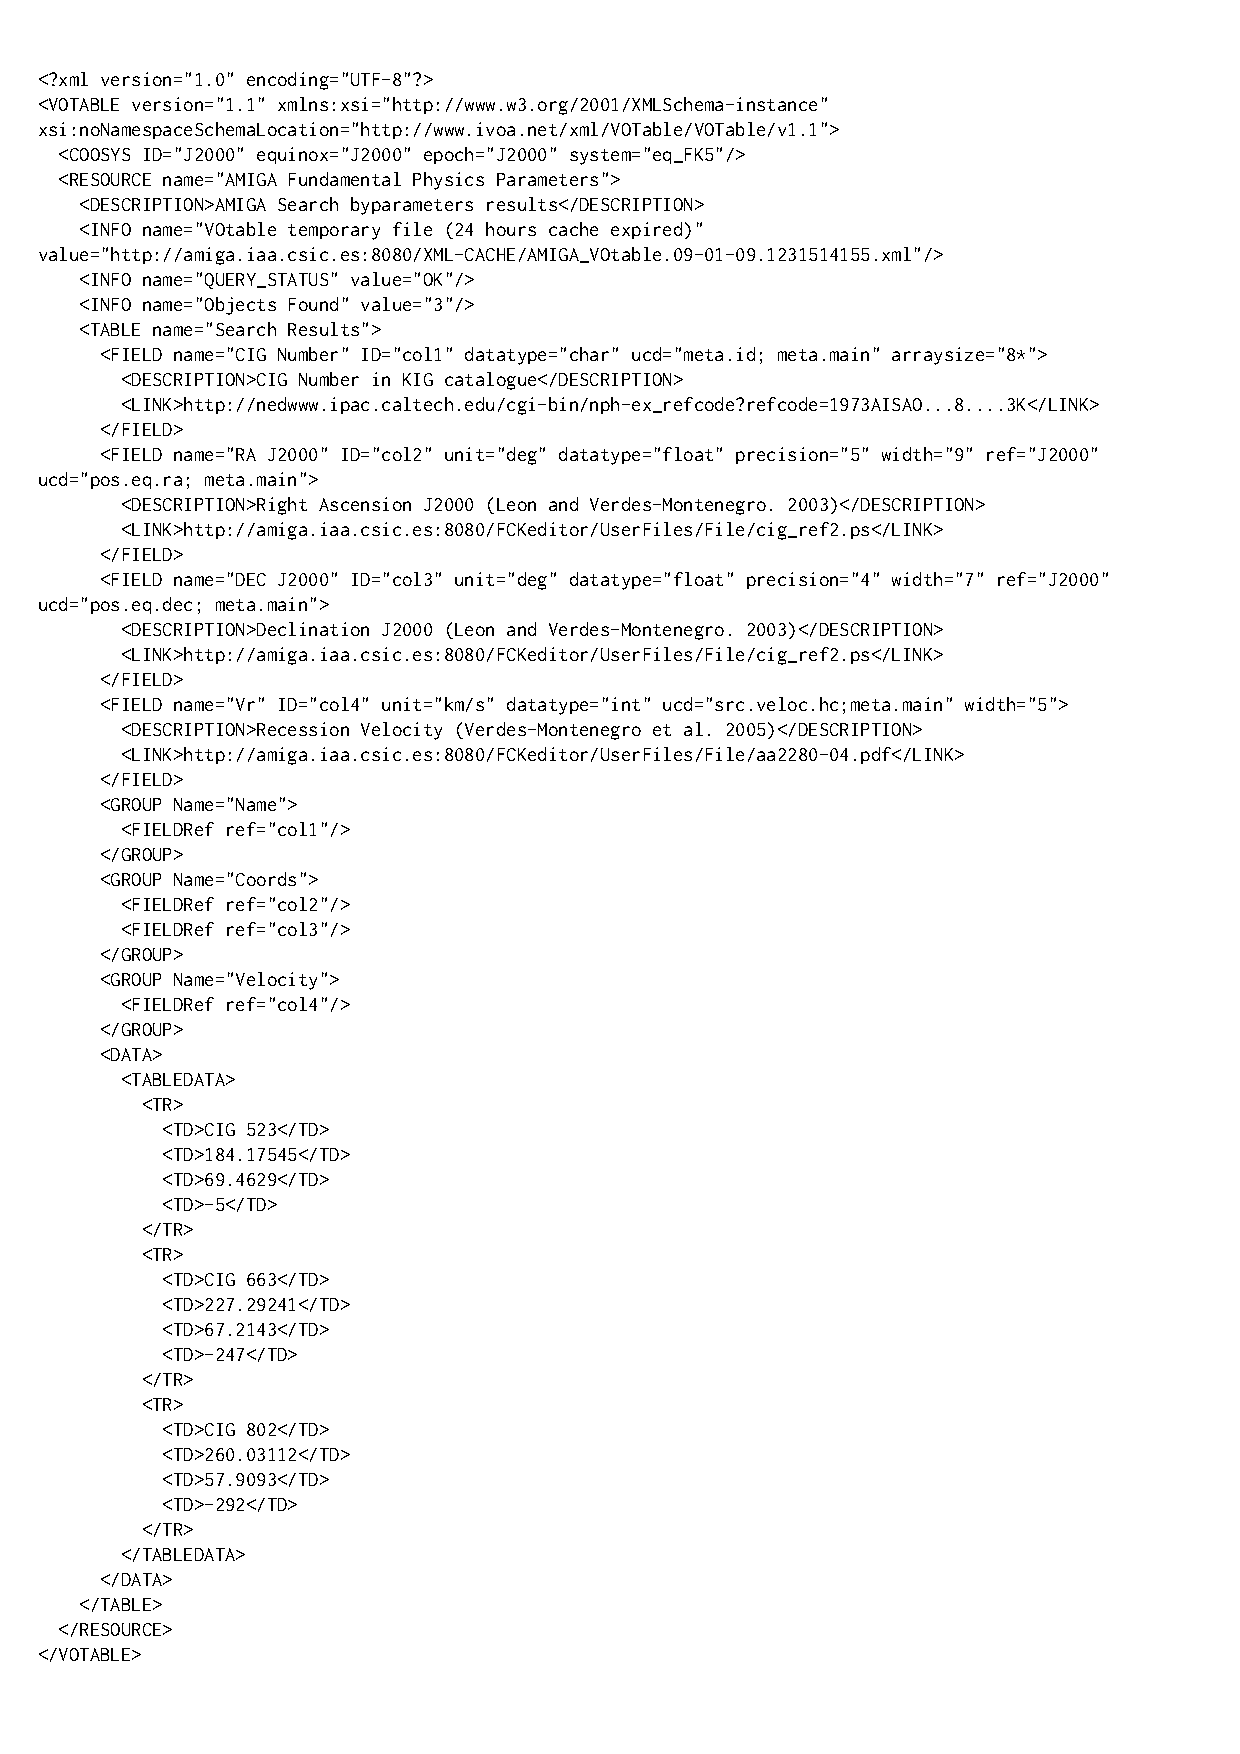
\includegraphics[height=0.787\textheight]
					{fig/amiga-vot.pdf}
				\caption[VOTable example]{
					Example of VOTable obtained from the AMIGA
					catalogue VO interface,
					\url{http://amiga.iaa.csic.es/DATABASE/}. We
					can see that after the initial XML declaration,
					and opening the \xmltag{VOTABLE}, the
					\xmltag{COOSYS} is used to specify the
					coordinate system equinox and epoch, and then
					the data is described in the
					\xmlopen{RESOURCE}/\xmltag{TABLE}. The
					\xmltag{FIELD} is used for every column in the
					table, the \xmltag{GROUP} is used to group
					together related fields, and then the
					\xmlopen{DATA}/\xmltag{TABLEDATA} contains the
					table rows between \xmltag{TR}s, and with
					columns separated by the \xmltag{TD}.
				}
				\label{fig:fig_amiga-vot}
			\end{figure}
					
			The complete definition of the VOTable, in terms of its
			XML Document Type Definition (DTD), and an XML Schema,
			can be found in
			appendix~\ref{cha:votable_format_definition}.
		
		% subsection the_votable (end)

%	The FITS file format intended to address two problems at the
%	time: standardising a data format for astronomical image and
%	tabular data interchange, and providing a computer
%	tape-friendly storage mechanism, with support for record
%	lengths multiple of common record lengths at the time.


%	, and in order to do that practically data had to be digitally
%	sampled. In fact, interferometry data conform a sparse sampling
%	of what is called the visibility plane, and imaging is made by
%	applying the Fourier Transform to that sparse sample. Models on
%	the originating data have to be imposed in order to do a proper
%	image reconstruction, and algorithms such as CLEAN, or Maximum
%	Entropy have been devised for that reconstruction.

	% section vo_data_formats (end)

	\section{VO data access protocols} % (fold)
	\label{sec:vo_data_access_protocols}
		
		The common file format helps in the data interchange
		between different systems, and in letting different
		applications share data. However, in order to retrieve
		those data from the different archives existing in the VO,
		common data access protocols are needed.
		
		 Then main astronomical data products produced as
		astronomical observation facilities are the reduced image,
		and the reduced 1D spectra. Working with those images and
		spectra, different properties of objects in the universe,
		such as temperature, distance, diameter, or more directly,
		received flux, Point Spread Function (PSF), et cetera, can
		be derived, and positional catalogues created.
		
		 For those kinds of data the initial VO protocols to be
		created were the Simple Image Access
		Protocol~\cite{2008sia..rprt.....T} (SIAP) and the Simple
		Spectral Access
		Protocol~\cite{Tody:2007yq,2004SPIE.5493..262D} (SSAP). For
		catalogues the Simple Cone Search (SCS, or ConeSearch)
		protocol~\cite{Williams:2008fv} was devised, with the idea
		of retrieving table rows from positional catalogues centred
		around a certain position, and from a certain angular
		distance from the centre (hence the Cone in the protocol
		name).
		
		 Apart from data-product driven access protocols, an
		additional data access protocol is needed for querying the
		VO Registry. That protocol is based on the Open Archives
		Initiative
		
		 You can find a brief description of each protocol
		interface in appendix~\ref{cha:vo_protocols} for quick
		reference.
		
	% section vo_data_access_protocols (end)

	\section{VO data models} % (fold)
	\label{sec:vo_data_models}
		
		With a common data format and a common data access protocol
		astronomers would be able to access different archives
		using automated tools, and the data could be sent to
		different applications.
		
		 However, astrophysical datasets are very complex in
		nature, and with the flexibility of the VOTable or the FITS
		file formats many different files can be constructed which
		contain the same astrophysical information, but in a
		incompatible form.
		
		 A data model is a description of the set of entities
		needed for information storage in a particular field, and
		specifies both the data being stored, and the relationships
		between them.
		
		 For the VO, there are several kinds of data models which
		can be built:
		
		\begin{description}
			\item[A general data model for astronomical
			observations] one such data model would be centred around
			the idea of astronomical observation and data reduction
			setup.
			
			 \item[Data model for individual data products] these
			data data models would exist for the different data
			products created with the different astronomical
			instruments: images, spectra, data cubes (collections
			of images or spectra), photometric data, et cetera.
		\end{description}
		
		In order to identify that a particular datum, appearing
		anywhere in a VO dataset, has a precise astronomical
		meaning the Unified Content Descriptors (UCDs) where
		created. They conform a controlled vocabulary whose precise
		meaning is set by the IVOA, and allow, for instance, to
		identify if a table column corresponds to flux in a
		particular radio band, or provides an astronomical
		coordinate, and so on.
		
		 We will see in Part~\ref{partRadioDataModelling} that the
		data modelling effort is still ongoing within the VO, and
		one of the main contributions of this thesis is a complete
		observation data model for radio astronomy, with some parts
		usable for non radio astronomical observations. More detail
		in UCDs will be offered there.

		%For instance, image mosaics can be delivered by a collection
		%of images in the same file with WCS information for each one;
		%or as a data cube with a different plane for each one of the
		%images, with a separate coordinates table related to each
		%plane; as a list of pixels with coordinates; as a series of
		%tables containing image data... the astronomical information
		%is the same, but we need to specify the kind of dataset
		%(astronomical image mosaic), and the relationship
		%
		%The VO needs, then, to be sufficiently structured so that
		%different applications and services provide the same metadata
		%for the same kind of data products, so that all applications
		%which know how to operate on certain datasets (images or
		%spectra, for instance, but also astronomical catalogues)
		%can find all the metadata they need for their operations.
		
		

		
		%There are two main kinds of astronomical data:
		%
		%\begin{description}
		%	\item[Data from observations] These are the most related
		%	to astronomical infrastructure. These are data coming from
		%	instruments in all kind of telescopes, and basically
		%	consist of the (more or less processed) output from light
		%	detectors.
		%	
		%	\item[Astronomical catalogues] Lists of astrophysical
		%	properties related to positions of the sky, which have been
		%	derived upon careful processing of observational data.
		%	These include purely physical parameters, such as
		%	temperatures, densities, masses, fluxes in different bands,
		%	et cetera; or attributes related with the observed object,
		%	such as object kind, morphology, names in pther catalogues,
		%	or even with the observational setup.
		%\end{description}
		%
		%%In astronomical observatories data is mainly in the form of
		%%observational data, but typically a catalogue of observed
		%%objects is generated.
		%%For surveys, the data is processed by an
		%%automatic processing pipeline which provides many different
		%%astronomical catalogues.
        %
		%As catalogue data is tabular in nature, the VOTable is a
		%perfect format for their distribution. However, they comprise
		%many diverse physical parameters, and it is very useful to
		%combine different catalogues to complement the physical
		%information. For instance, if we have infrared fluxes for an
		%object (from observations from an IR satellite, for instance),
		%but optical fluxes exist for the same object in a different
		%catalogue (from a ground based telescope, perhaps), combining
		%them will extend our knowledge of what is called the Spectral
		%Energy Distribution (SED)
		%of that object, and will helps in our
		%understanding of that object.
		%
		%In this case, we have three different problems to solve:
		%
		%\begin{enumerate}
		%	\item finding out catalogues which contain our object;
		%	
		%	\item cross-matching the catalogues, so that we can find
		%	out which objects in one catalogue correspond to the same
		%	object in other catalogue; this is implies being able to
		%	recognize in catalogues:
		%	
		%	\begin{itemize}
		%		\item which columns are devoted to astronomical 
		%		coordinates;
		%		\item find objects at a distance compatible with the
		%		precision of the astronomical coordinates
		%		(cross-matching);
		%	\end{itemize}
		%	
		%	\item identify exactly which properties are found in each
		%	column.
		%\end{enumerate}
		

		

		
	%	\todo{Revise the idea of semantics}
	%	We have talked several times about how VOTables, the common
	%	IVOA data format, allows data providers to specify data models
	%	and semantics for particular columns.
    %
	%	We understand semantics as the set of metadata which is used
	%	to allow automatic discovery of data roles. Part of that
	%	semantics come from the particular field where the data is
	%	being generated or applied, and are coded into the particular
	%	data model applied to the field.
    %
	%	In the VO, there are three kinds of attributes devoted to
	%	provide semantics to tagged data in VOTables: units, UCDs, and
	%	UTypes.
    %
	%	\subsection{Units} % (fold)
	%	\label{sub:units}
    %
	%	Mathematical operations on physical quantities can only be
	%	consistently performed on unit-compatible fields. For a
	%	tabular data and astrophysical image transport mechanism,
	%	be it FITS or VOTable, specifying the units for the
	%	different fields or pieces of data is almost mandatory.
	%	Even when the FITS standard does not mandate units to be
	%	provided, it recommends their use. In the same spirit, the
	%	unit attribute for VOTable tags is not mandatory, but it is
	%	strongly recommended.
    %   
	%	There is also a provision for constructing dimensional
	%	equations and other string units, but several equivalent
	%	ways of specifying those equations are allowed, instead of
	%	establishing an unambiguous construction rule.
    %   
	%	Within the Virtual Observatory, the Semantics Working
	%	Group has a dedicated group to Units.
	%	\textbf{Pedro Osuna and Jesús Salgado}
	%	made a concrete proposal for uniquely specifying
	%	both units and dimensional equations in the context of
	%	astrophysical spectra~\cite{2005astro.ph.11616O}.
    %   
	%	In particular, they proposal makes use of the Dimensional
	%	Analysis in order to show that, more than simple units, the
	%	dimensional equation, and scaling factors with respect to
	%	SI (System Internationale) units,
	% are enough to allow automatic comparison and
	%	re-scaling and interoperation between spectra with either
	%	frequency or wavelength units, 
	%	and flux densities with respect to
	%	frequency or wavelength (a non trivial task). Additional
	%	\texttt{dimeq} and \texttt{scaleq} attributes for specifying
	%   unit scales and dimensional equations in a
	%	VOTable, or \texttt{CSCALEQ} and \texttt{CDIMEQ} FITS
	%	keywords have to be added for each axis to provide unit
	%	interoperation.
    %   
	%	They have already implemented their recommendation in
	%	their VOSpec spectral analysis and SED synthesis tool, in
	%	order to be able to assemble spectral energy distributions
	%	from spectra in the whole emission range, from radio to
	%	X-rays. In that sense, errors must also be provided, with
	%	their corresponding units.
    %   
	%	Dimensional analysis is key for unit semantics in the
	%   Virtual Observatory data. With access to
	%	dimensional equations, automatic data mining of properties
	%	of large samples can derive a reliable functional fit of
	%	the dependency between observable quantities, by obtaining
	%	the independent adimensional products of observable
	%	parameters, and testing different functional forms of those
	%	adimensional products for the best fit to observational
	%	data~\cite{2007arXiv0709.3584T}.
    %
	%	% subsection units (end)
    %
	%	\subsection{Unified Content Descriptors (UCDs)} % (fold)
	%	\label{sub:unified_content_descriptors}
	%		
	%	Specifying both units and the unit reference base (usually,
	%	the SI, but many times, and for specific areas of
	%	astrophysics such as cosmology or high energy astrophysics,
	%	other unit base systems are adopted) is mandatory to allow
	%	commensurable data to be compared.
	%	
	%	However, many times quantities of the same nature, but
	%	different origin, coexist in the same table. For instance,
	%	one might have a table of flux measured at several
	%	wavelengths. All columns will share the same flux units
	%	(or, in any case, they can be automatically converted by
	%	means of dimensional attributes), but have a different
	%	meaning for an astrophysicist. Distinguishing between
	%	unit-compatible fields with different astrophysical meaning
	%	is the role of the UCDs~\cite{2004ASPC..314..315D}.
	%	
	%	UCDs were developed for the
	%	VizieR\urlnote{http://vizier.u-strasbg.fr/} online
	%	astronomical catalogue storage and query
	%	system~\cite{2000A&AS..143...23O} in the context of the
	%	ESO/CDS data mining project~\cite{1999ASPC..172..379O}, in
	%	order to harmonise the labelling (semantics) of similar
	%	fields between catalogues submitted from different research
	%	groups across the world\footnote{A classical example is the
	%	labelling of magnitudes in the V filter of the Johnson
	%	photometric system. Prior to the introduction of UCDs,
	%	there were up to 150 different labels for columns including
	%	information of that magnitude.}. Only if truly equivalent
	%	columns are compared can knowledge be reliably extracted.
	%	By using a controlled vocabulary, it is possible to find
	%	comparable information from different sources (for
	%	performing statistics on large samples, for instance).
	%	
	%	Still, even when UCDs are truly useful when comparing
	%	catalogues, and are very
	%	\textbf{interesting} for the discovery of
	%	what information might be comparable, they are not enough
	%	for specifying the role of a given datum in a larger
	%	context. For that, we need data models, and a way to
	%	specify relationships of a single datum with data model
	%	entities and attributes.
	%		
	%	% subsection unified_content_descriptors (end)
    %
	%   \subsection{Data models in the VO} % (fold)
	%   \label{sub:data_models_in_the_vo}
    %
	%   \todo{
	%   	\begin{itemize}
	%   		\item Existing VO data models
    %
	%   		\begin{itemize}
	%   			\item Characterisation
    %
	%   			\item Spectrum/Spectral Energy Distribution
	%   		\end{itemize}
    %
	%   		\item Missing VO Data Model classes
    %
	%   		\begin{itemize}
	%   			\item Provenance
	%   			\item Policy
	%   			\item Packaging
	%   			\item Target
	%   			\item Observation
	%   		\end{itemize}
    %
	%   		\item New VO Data models in this thesis
    %
	%   		\begin{itemize}
	%   			\item Provenance
	%   			\item Policy
	%   			\item Packaging
	%   		\end{itemize}
    %
	%   		\item RADAMS
	%   	\end{itemize}
	%   }
			
			
			
		% subsection data_models_in_the_vo (end)


	% section sec:vo_data_models (end)

	\section{VO applications} % (fold)
	\label{sec:vo_applications}

		VO data formats, access protocols, and data models are the
		infrastructure on which the rest of the VO relies. We
		call \emph{VO application} to any software package of any
		kind which makes use of existing VO services to perform
		the visualisation of data in VO format, queries of VO
		services, or even computations on existing datasets either
		in VO format, or retrieved from the VO.
		
		 However, having VO users in mind, it is best to classify
		applications depending on whether they allow users and/or
		developers to create new packages, or if they are intended
		to be used for scientific analysis. And in this latter
		case, the kind of scientific use they support.
		
		 We have provided a series of tables with a non-exhaustive
		list of different classes of VO applications:
		table~\ref{tabVODataDiscoveryApps} compiles VO applications
		for data discovery; table~\ref{tabVODataHandlingApps}
		combines applications for data manipulation and handling;
		VO applications specific for spectral analysis are shown in
		table~\ref{tabVOSpectralApps}; table~\ref{tabVODevelTools}
		shows tools, libraries, and reference portals to the VO for
		application developers; finally, difficult to classify VO
		resources can be found in table~\ref{tabVOotherApps}.
		
	 	%%todo (fold)
		%\todo{
		%	For each of these....
		%	\begin{itemize}
		%		\item Registry queries
		%		\item ConeSearch queries
		%		\item SIAP queries
		%		\item SSAP queries
		%	\end{itemize}
	    %
		%	Specify:
		%	\begin{itemize}
		%		\item Application name
		%		\item URL
		%		\item Strengths
		%		\item Weaknesses
		%	\end{itemize}
		%}
		%%todo (end)

			\newcommand{\ivoaappsurl}
	{\concatenate{http://www.ivoa.net/cgi-bin/}
	{twiki/bin/view/IVOA/IvoaApplications}}
	\newcommand{\fromlist}
	{
		from the \href{\ivoaappsurl}{IVOA},
		\href{http://www.us-vo.org/projects/tools.cfm}{NVO} and
		\href{http://www.euro-vo.org/pub/tc/software.html}{EuroVO
		TC} applications and tools' lists.
	}
	
	\begin{table}
	\begin{center}
	\begin{scriptsizetabular}{p{2.8cm}p{9.5cm}}
	
	\textbf{Application} &
	% \textbf{Contact Person} &
	\textbf{Description} \\ \midrule
	
	\href{http://aladin.u-strasbg.fr/} {Aladin} & Interactive
	federated sky atlas.\\ \addlinespace
	
	\href{http://heasarc.gsfc.nasa.gov/vo} {NVO Datascope} & 
	Portal for positional queries to all NVO registered services.
	\\ \addlinespace
	
	\href{http://www.cadc-ccda.hia-iha.nrc-cnrc.gc.ca/cvoProto/}
	{Octet} & CVO Registry Observation CaTalog Exploration Tool.
	% Queries the CVO registry, provides data cross-matching.
	\\ \addlinespace
	
	\href{http://www.astrogrid.org/wiki/Help/IntroVODesktop}
	{VODesktop} & A resource-centered desktop client for VO:
	includes VOExplorer, Query and Task Runner, Astroscope, VOSpace
	Browser, Astro Runtime. \\ \addlinespace
	
	\end{scriptsizetabular}
	\end{center}
	\caption[List of VO data discovery applications]
	{List of VO data discovery tools and applications, \fromlist}
	\label{tabVODataDiscoveryApps}
	\end{table}
	
	
	\begin{table}
	\begin{center}
	\begin{scriptsizetabular}{p{2.8cm}p{9.5cm}}
	
	\textbf{Application} &
	% \textbf{Contact Person} &
	\textbf{Description} \\ \midrule
	
	\href{http://www.cacr.caltech.edu/projects/nvo/atlasmaker/3}
	{Atlasmaker} & Grid software for bulk image resampling.\\
	\addlinespace
	
	\href{http://cm.bell-labs.com/who/tkh/mirage/index.html}
	{Mirage} & Multi-dimensional visualisation of data from VOTable
	source files.\\ \addlinespace
	
	\href{http://montage.ipac.caltech.edu/} {Montage} &
	Science-grade custom mosaics from a portal.\\ \addlinespace
	
	\href{http://iraf.noao.edu/projects/vo/votool/} {NOAO VOTool} &
	A visual VOTable authoring and editing tool. \\
	\addlinespace
	
	\href{http://iraf-nvo.noao.edu/wcsfixer/} {NOAO WCSFixer} &
	Automatic WCS correction for uploaded images. \\ \addlinespace
	
	\href{http://www.atnf.csiro.au/vo/rvs} {Remote Visualisation
	System (RVS)} & Distributed software for visualisation and
	analysis of remotely located astronomical images with VO
	support. \\ \addlinespace
	
	\href{http://www.star.bristol.ac.uk/~mbt/topcat/} {TOPCAT} &
	Viewer and editor for tabular information. Based on the
	STILTS tool set.\\ \addlinespace
	
	\href{http://www.starlink.ac.uk/treeview/} {Treeview} &
	Hierarchical data format viewer with XML and
	VOTable support. \\ \addlinespace
	
	\href{http://visivo.cineca.it/} {VisIVO} & A VO-compatible
	visualisation tool for large datasets. \\ \addlinespace
	
	\href{http://vo.iucaa.ernet.in/~voi/voplot.htm} {VOPlot} &
	Tool for visualizing astronomical data from VOTable sources.\\
	\addlinespace
	
	\href{http://services.china-vo.org/vofilter/} {VOFilter} & XML
	filter for OpenOffice Calc to Read/Write VOTable Files.\\
	\addlinespace
	
	\href{http://services.china-vo.org/votable2xhtml/}
	{VOTable2XHTML} & XSLT Style-sheet for exporting VOTable files
	to HTML.  \\
	\addlinespace
	
	\href{http://nvogre.phyast.pitt.edu:8080/wesix/} {WESIX} &
	\emph{Web Enabled Source Identification with X-matching},
	portal for image upload, source extraction, and cross
	correlation with selected survey catalogues.
	
	\end{scriptsizetabular}
	\end{center}
	\caption[List of VO data handling and manipulation
	applications]
	{List of VO data handling and manipulation applications,
	\fromlist}
	\label{tabVODataHandlingApps}
	\end{table}
	
	
	
	\begin{table}
	\begin{center}
	\begin{scriptsizetabular}{p{2.8cm}p{9.5cm}}
	
	\textbf{Application} &
	% \textbf{Contact Person} &
	\textbf{Description} \\ \midrule
	
	\href{http://voplus.obspm.fr/~chil/Euro3D/}
	{Euro3D} & Spectral analysis tool for Euro3D formatted
	Integral Field Units (IFUs) datasets, by Igor
	Chilingarian.\\
	\addlinespace
	
   \href{http://www.stsci.edu/resources/software_hardware/specview}
	{Specview} & Visualisation and analysis tool for 1-D
	astronomical spectrograms.\\ \addlinespace
	
	\href{http://star-www.dur.ac.uk/~pdraper/splat/splat-vo/}
	{SPLAT} & Spectral Analysis Tool from Starlink. \\
	\addlinespace
	
	\href{http://svo.laeff.inta.es/theory/vosa2//}{VOSA} &
	A web-based tool developed by the SVO for automatic
	analysis of
	Spectral Energy distributions from online spectra.\\
	\addlinespace
	
	\href{http://sdc.laeff.inta.es/vosed/}{VOSED} & A web-based
	tool
	developed by the SVO for
	building Spectral Energy distributions from online spectra.\\ 
	\addlinespace
	
	\href{http://www.star.bris.ac.uk/~mbt/yafit/}{Yafit} & Yet
	Another Fitting tool for fitting curves to data points,
	which can be used to fit model spectra to observed photo
	metric data points, by Mark Taylor.\\ 
	\addlinespace
	
	\newcommand{\sciopsbaseurl}[0]
	{http://www.sciops.esa.int/index.php}
	\href{\sciopsbaseurl?project=ESAVO}{VOSpec} &
	A Tool to Handle VO-SSAP compliant spectra.\\ \addlinespace
	
	\end{scriptsizetabular}
	\end{center}
	\caption[List of VO spectral analysis and SED fitting
	applications]
	{List of VO applications for spectral analysis and
	spectral energy distribution (SED) fitting, \fromlist}
	\label{tabVOSpectralApps}
	\end{table}
	
	
	
	
	\begin{table}
	\begin{center}
	\begin{scriptsizetabular}{p{2.8cm}p{9.5cm}}
	\textbf{Developer Tool} &
	% \textbf{Contact Person} &
	\textbf{Description} \\ \midrule
	
	\newcommand{\arpythonurl}[0]
	{\concatenate{http://deployer.astrogrid.org/software/}
	{astro-runtime/commandline/index.html}}
	\href{\arpythonurl}
	{AR Command line} & Python wrapper for the AstroRuntime
	VO middleware. \\ \addlinespace
	
	\href{http://cdsweb.u-strasbg.fr/cdsdevcorner/} {CDS Developer's
	Corner} & Web site for developers of the Centre de Donées de
	Strasbourg, where references to CDS web-services and CDS Java
	software can be found, including unit handling. \\
	\addlinespace
	
	\href{\jsampurl}
	{JSAMP} &
	JSAMP is a Java implementation of the SAMP messaging
	protocol written in Java by Mark Taylor.\\
	\addlinespace
	
	\href{\caltechphpurl}{PHP VO Client Library} & 
	PHP interface classes to ConeSearch, SIAP, SkyNode,
	and VORegistry services.\\
	\addlinespace
	
	\href{\caltechpythonurl}{Python VO Client Library} &
	Python interface classes to ConeSearch, SIAP, SkyNode,
	and VORegistry services.\\
	\addlinespace
	
	\href{http://amwdb.u-strasbg.fr/saada} {Saada} &
	Auto-configurable database generator and VO Service publisher
	for medium to small sized datasets, directly from FITS files.
	\\ \addlinespace
	
	\href{\sampyurl}
	{SAMPy} & SAMPy is a Python implementation of the SAMP
	messaging protocol, with additions to allow for SAMPy
	applications to communicate with remote computer, and not just
	locally. By Luigi Paioro.\\
	\addlinespace
	
	\href{http://cdsweb.u-strasbg.fr/cdsdevcorner/savot.html}
	{SAVOT} &
	Simple Access to VOTable, SAVOT is a Java-based library to
	parse VOTable documents, written by André Schaaff from the
	CDS.\\
	\addlinespace
	
	\href{\stiltsurl} {STILTS} &
	Command-line tools for arbitrarily large table manipulation
	and format conversion, including FITS and VOTable formats.
	By Mark Taylor.\\
	\addlinespace
	
	\href{http://iraf-nvo.noao.edu/vo-cli/} {VO-CLI} &
	Command-line Tools for the VO, to be used with IRAF. \\
	\addlinespace
	
	\end{scriptsizetabular}
	\end{center}
	\caption[List of VO development resources]
	{List of VO developer utilities, libraries, and resources,
	\fromlist}
	\label{tabVODevelTools}
	\end{table}
	
	\begin{table}
	\begin{center}
	\begin{scriptsizetabular}{p{2.8cm}p{9.5cm}}
	
	\textbf{Application} &
	% \textbf{Contact Person} &
	\textbf{Description} \\ \midrule
	
	\href{http://bima.astro.umd.edu/nemo/tvo/nvodemo2004/} {GC
	Theoretical Models} & Prototype tool for comparing
	globular cluster (GC) simulations with observed
	color-magnitude diagrams.\\ \addlinespace
	
	\href{http://www.nvo.noao.edu} {NOAO NVO Portal} &
	VO portal providing different views for NOAO-hosted data.
	%Provides a unified UI for different archives, including
	%calendar and footprint views.
	\\ \addlinespace
	
	\href{http://pegasus.isi.edu/} {Pegasus} & Workflow Management
	on the Grid.\\ \addlinespace
	
	\href{http://hea-www.harvard.edu/~arots/nvometa/} {STC
	Metadata} & Space-Time Coordinate metadata for the VO.\\
	\addlinespace
	
	\href{http://voservices.org/} {VO Services} & A growing
	selection of VO services in production.\\ \addlinespace
	
	\href{http://nvogre.phyast.pitt.edu:8080/wesix/} {WESIX} &
	\emph{Web Enabled Source Identification with X-matching},
	portal for image upload, source extraction, and cross
	correlation with selected survey catalogs.
	
	\end{scriptsizetabular}
	\end{center}
	\caption[List of other VO applications and portals]
	{Other VO applications and portals not presented yet, \fromlist}
	\label{tabVOotherApps}
	\end{table}
	

	% section vo_applications (end)

	\section{VO inter-application messaging} % (fold)
	\label{sec:vo_application_messaging}
	
		The data access protocols mentioned in
		section~\ref{sec:vo_data_access_protocols} need the
		deployment of a full-featured web server. However, in a
		local machine, with several VO applications running at the
		same time, and with all of them understanding VOTables and
		FITS files, a simple messaging protocol between
		applications would allow them to notify, or be notified,
		that some data is available, and if the messaging protocol
		supported it, several applications in communication could
		be showing different but interacting views of the same
		data.
		
		 Such a messaging protocol was prototyped and was initially
		known as the PLatform for Astronomical Tool InterConnection
		(PLASTIC), and implemented in many different VO
		applications, such as TOPCAT, or the Aladin Sky Atlas. The
		shortcomings of the PLASTIC protocol gave birth to the
		Simple Application Messaging Protocol (SAMP), now in
		Proposed Recommendation stage.
		
		 The SAMP messaging protocol is described in
		section~\ref{sec:samp_messaging}.
	
	% section vo_application_messaging (end)
	
	\section{VO resource registry} % (fold)
	\label{sec:vo_resource_registry}
	
		The only way VO clients can remain aware of existing and
		newly incorporated services is by means of a registration
		point were public data services are announced.
		
		 In the VO, there is no centralised, preferential registry.
		Instead, many registries exist, but with the ability to
		harvest entries from other registries, so that there can
		exist specialised registries on one hand, and shared
		registries entries on the other.
		
		 VO registry and harvesting infrastructure has been built
		around the Open Archives
		Initiative\urlnote{http://www.openarchives.org/} (OAI)
		standard resource registries, so that an already in place
		infrastructure could be leveraged. The OAI has developed a
		Protocol for Metadata Harvesting
		(OAI-PMH)~\cite{2002OAI-PMH}, that allows OAI registries to
		harvest other OAI registries they might know about (with an
		entry in their own registry, for instance), so that VO
		resources can be entered in one registry, and they should
		propagate to any other OAI-PMH compliant registries.
		
		 That allows VO tools to point to a single harvesting
		registry, and rest assured that VO servers will be found in
		any of those registries.
		
		 Registered resources (OAI-PHM records) provide at least
		the Dublin Core metadata set~\cite{2007NISO.Z3985...K},
		which specifies resource types, publishers, curators, et
		cetera.
		%See table~\ref{tab:DublinCoreMetadata}
		%for the complete list of Dublin Core keywords.
		Additionally, service-specific resource profiles exist for
		the different data access service types, and include
		astronomical data for service such as the sky region
		covered by the observation ---footprint---, wavelength,
		instruments providing the data, et cetera.
		
		 In particular, the VOResource~\cite{2008voresivoar0222P}
		XML Schema has been developed as the acceptable OAI-PHM
		record formats for generic VO registries, and the
		VODataService schema~\cite{2008vods.ivoar1016P} is in
		development to further standardise data service entries.
		
		 Several VO registries provide web pages to query the
		registries apart from the usual OAI-PHM interface, such as
		the NVO
		Carnivore\urlnote{http://nvo.caltech.edu:8080/carnivore/},
		or the ESA-VO
		registry\urlnote{http://esavo.esa.int/registry/}.
	
	% section vo_resource_registry (end)
	
	% section the_international_virtual_observatory_alliance (fold)
	\section[The International Virtual Observatory Alliance]
	{Standardising the VO:
	 the International Virtual Observatory Alliance (IVOA)}
	\label{sec:the_international_virtual_observatory_alliance}

		% \lourdes{Buscar sitio para párrafo intro IVOA.}
		As previously stated, for VO common data formats,
		interfaces, and data models to become truly standard
		requires a standards enforcing authority, and within the VO
		the International Virtual Observatory Alliance (IVOA) is
		the organisation in charge of developing and sanctioning
		interoperability standards.
		
		 The International Virtual Observatory Alliance was created
		in 2002, after the first national VO associations realised
		that they needed to keep working together, and that an
		international standards-setting organisation was needed to
		sanction Virtual Observatory standards, steer the
		development of new ones, and foster the spread of the VO to
		most data providers.
		
		 The IVOA founders were the US National Virtual Observatory
		(NVO), the European (AVO) and supporting centres ---Centre
		de Données astronomiques de Strasbourg (CDS), AstroGrid,
		German Astrophysical Virtual Observatory (GAVO)---, the
		Russian Virtual Observatory (RVO), VO-India, e-Astronomy
		Australia (eAA; later Australian Virtual Observatory,
		Aus-VO) and the Canadian Virtual Observatory (CVO), which
		in 2002 met at the ESO Headquarters in Garching, and agreed
		in forming the International Virtual Observatory Alliance,
		following the statement drafted by Peter Quinn, Robert
		Hanisch, and Andy Lawrence~\cite{Quinn:2002qf}. The minutes
		of that meeting can be found in~\cite{deYoung:2002rt},
		and the conference proceedings compiled in the book
		\emph{Toward an International Virtual
		Observatory}~\cite{2004tivo.conf.....Q}.
		
		 Following that initial meeting, several services were
		created, and Aladin was provided with a VO interface,
		giving birth to the first Astrophysical Virtual Observatory
		(AVO) prototype~\cite{2004ASPC..314..304Q}.
		
		 The inspiration for the IVOA organisation is the World
		Wide Web Consortium\urlnote{http://w3c.org/} (W3C), in the
		sense of providing the steering effort for standards to be
		agreed upon within different Working Groups (WGs), so that
		there is an official forum in which such standards are
		proposed, discussed, and finally approved. The main
		difference with the W3C is that the latter is \emph{pay per
		play} ---W3C participants pay in order to influence the
		standardisation process---, while the IVOA is open to any
		interested party with expertise in a given field.
		
		Presently \invisiblenote{(as of August 2008)}, the IVOA is
		formed by 16 VO projects from all over the
		world\urlnote{http://ivoa.net/pub/members/}, from Armenia,
		Australia, Canada, China, Europe, France, Germany, Hungary,
		India, Italy, Japan, Korea, Russia, Spain, the United Kingdom,
		and the United States (see figure~\ref{fig:fig_IVOAMembers}).
		Membership is open to additional national and international
		projects\footnote{
			VO projects wishing to join the IVOA must
			follow the IVOA Guidelines for Participation
		\url{http://ivoa.net/Documents/latest/IVOAParticipation.html}.
		}.

		\begin{figure}[tbp]
			\centering
				
\includegraphics[width=\columnwidth]
				{fig/ivoa-members.png}
			\caption[IVOA member organisations]
			{
				The 16 IVOA member organisations, as of August
				2008. The Spanish Virtual Observatory (SVO) joined
				the IVOA in 2004. Several European countries have
				their own national VO initiatives (France's
				VO-France, Germany's GAVO, Italy's VObs.it, Spain's
				SVO, UK's AstroGrid), which also form part of the
				European Community funded Euro-VO.
			}
			\label{fig:fig_IVOAMembers}
		\end{figure}

		\newcommand{\svourl}[0]{http://svo.laeff.inta.es/}
		
		 The Spanish participation in IVOA is performed through the
		Spanish Virtual Observatory\urlnote{\svourl}
		(SVO)~\cite{2006ASPC..351...19G}. The seed for the SVO
		were the efforts of the Laboratorio de Astrofísica Espacial
		y Física Fundamental (Laboratory for Spatial Astrophysics
		and Fundamental Physics, LAEFF\footnote{LAEFF is part of
		the National Institute for Aerospatial Technologies, INTA})
		to build a VO-compliant archive from the IUE Newly
		Extracted Spectra (INES) archive\footnote{In fact, the VO
		INES archive was one of the first spectroscopic archives to
		be available to the VO.}.
		% Nowadays the main FTEs are provided by the
		% LAEFF-INTA (SVO-core), but additional FTEs are provided by
		% other partners, such as the IAA-CSIC, and there is a national
		% network which funds the participation of additional research
		% groups within the Virtual Observatory.
		This thesis is part of the IAA contribution to the SVO.
		
		 As mentioned earlier, the IVOA is a standards-sanctioning
		organisation and a steering force for the development of
		interoperability protocols, applications, and best
		practices regarding the Virtual Observatory. As seen on
		previous sections, there are different development areas
		within the VO, and there exist several Working Groups
		focused in each particular area. There are also Interest
		Groups which do not focus in actual development, but
		instead serve as a discussion forum for issues not directly
		pertaining to the Virtual Observatory, but which might
		eventually end up forming part of it.

		 The main IVOA organisational building blocks are Working
		Groups, Interest Groups, and Coordination and steering
		committees. Their detailed discussion can be found in
		Appendix~\ref{cha:the_ivoa}.
		Figure~\ref{OrganisationalBuildingBlocksIVOA} shows
		graphically the high-level organisation of the IVOA.
		
		\begin{figure}[tbp]
			\centering
				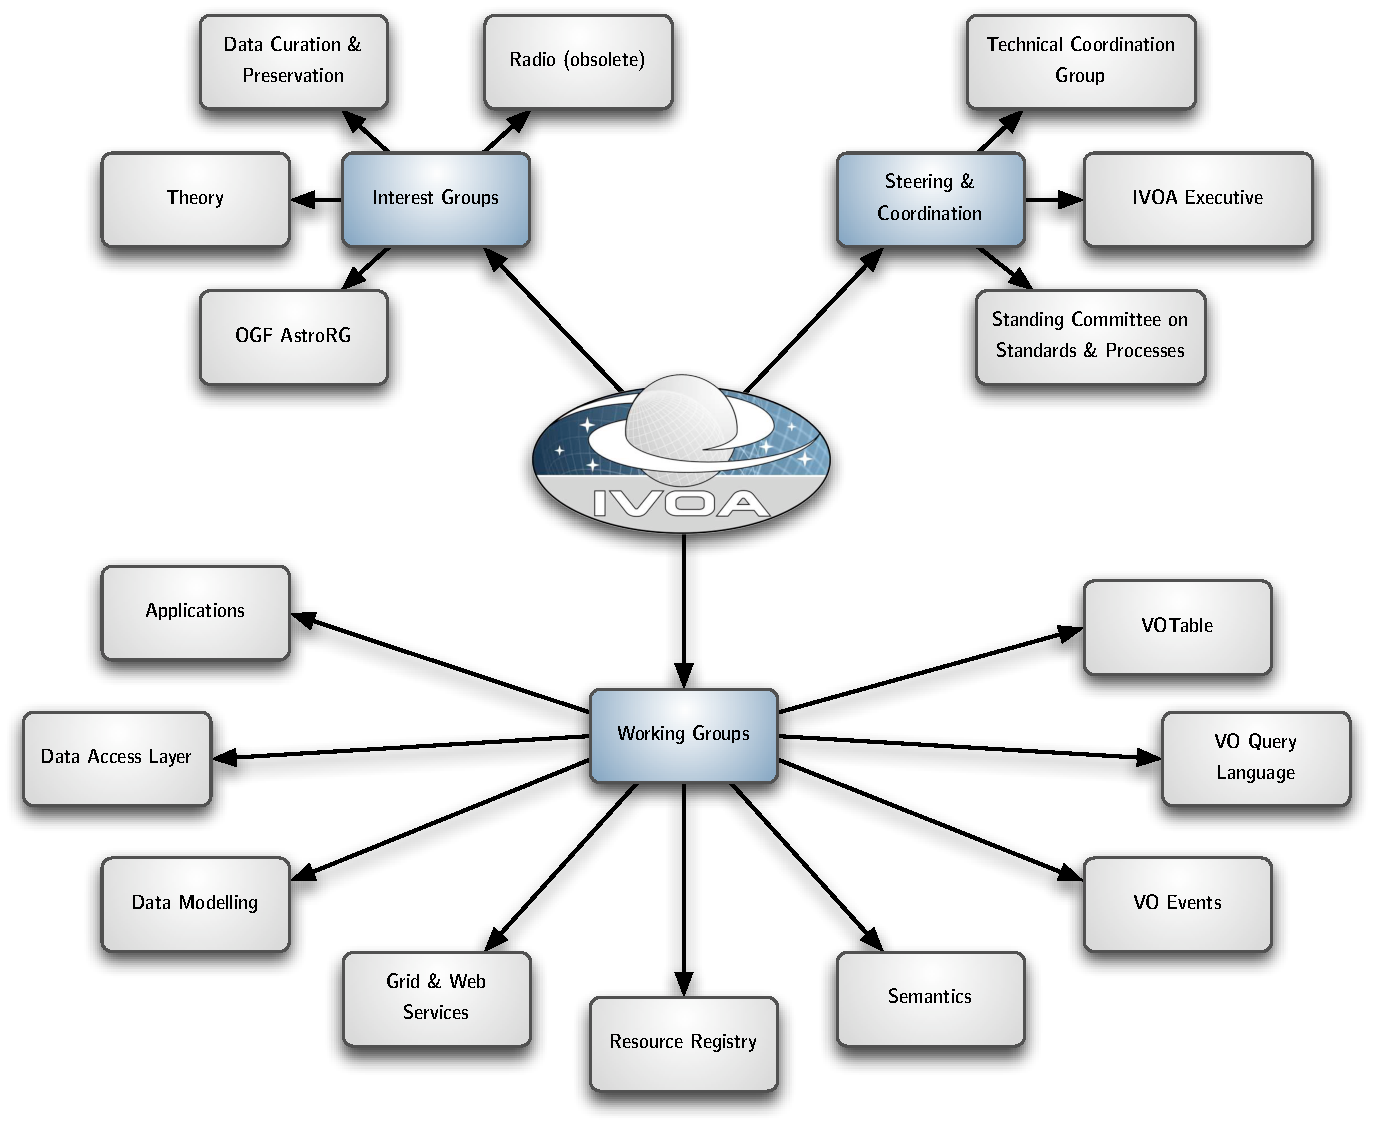
\includegraphics[width=\columnwidth]
				{fig/OrganisationalBuildingBlocksIVOA.pdf}
			\caption[IVOA organisational building blocks]{
				IVOA organisational building blocks: Working
				Groups, Interest Groups, and Coordination boards.
				The IVOA activity for standards development is
				performed in the Working Groups, while Interest
				Groups gather together IVOA users with common
				interests outside the Virtual Observatory (such as
				the Open Grid Forum, or the Data Curation and
				Preservation interest groups), or outside existing
				Working Groups (such as the Radio astronomy or or
				Theory interest groups). The Steering \&
				Coordination bodies provide the main direction for
				IVOA activities, technical coordination across the
				existing Working Groups (i.e., Data Modelling and
				Data Access Layer in the development of
				interoperable protocols and data set access tools),
				and take care of possible changes to existing
				standards.
			}
			\label{OrganisationalBuildingBlocksIVOA}
		\end{figure}
		
		IVOA Working Groups are not completely equal in scope. Most
		of them have to do with particular parts of the IVOA, as
		seen in figures~\ref{fig:fig_VOArch} and
		\ref{fig:fig_VOAPIStack}.
		
	% section the_international_virtual_observatory_alliance (end)


\section{The VO from the point of view of different actors} % (fold)
\label{sec:the_vo_from_the_point_of_view_of_different_actors}

	Which parts of the Virtual Observatory do users interact with?
	What does a particular astronomer need to know?
	
	 In the following subsections we will offer several portraits
	of the VO as seen from the points of view of different actors:
	the astronomical user, the application developer, the data
	provider, and the data service developer.

	\subsection{The VO from the user's point of view} % (fold)
	\label{ssub:the_vo_from_the_point_of_view_of_the_user}
	
	
		\newcommand{\specviewurl}[0]
		{http://www.stsci.edu/resources/software_hardware/specview}
		\newcommand{\splatvourl}[0]
		{http://astro.dur.ac.uk/~pdraper/splat/splat-vo/}
		\newcommand{\vodesktopurl}[0]
		{http://www.astrogrid.org/wiki/Install/Downloads}
	
		For a non-technical user (one who wishes to use the VO via
		standard tools, and does not wish to access directly the VO
		infrastructure), the VO can be seen just as a set of
		portals (applications or web sites) which access all of the
		services and data available in the Virtual Observatory.
		Some of them might also retrieve additional data from
		non-VO-compliant archives, and even mix them with local
		datasets. Users would launch different VO applications
		depending of the tasks they might wish to perform (Aladin
		Sky Atlas\urlnote{http://aladin.u-strasbg.fr/} for
		catalogue and image queries;
		TOPCAT\urlnote{http://www.star.bris.ac.uk/~mbt/topcat/} for
		catalogue and table manipulation;
		VOSpec\urlnote{http://esavo.esa.int/vospec/},
		SpecView\urlnote{\specviewurl} or
		SPLAT-VO\urlnote{\vodesktopurl} for spectra manipulation;
		VODesktop\urlnote{\vodesktopurl} for Registry queries,
		remote task execution, and access to the VOSpace; or web
		portals such as the NVO
		Datascope\urlnote{http://heasarc.gsfc.nasa.gov/vo/} for
		all-encompassing browser-based archive searches). See
		figure~\ref{fig:figUserPOV_VOArch} for a conceptual diagram
		of the VO for astronomers.
		
		\begin{figure}[btp]
			\centering
				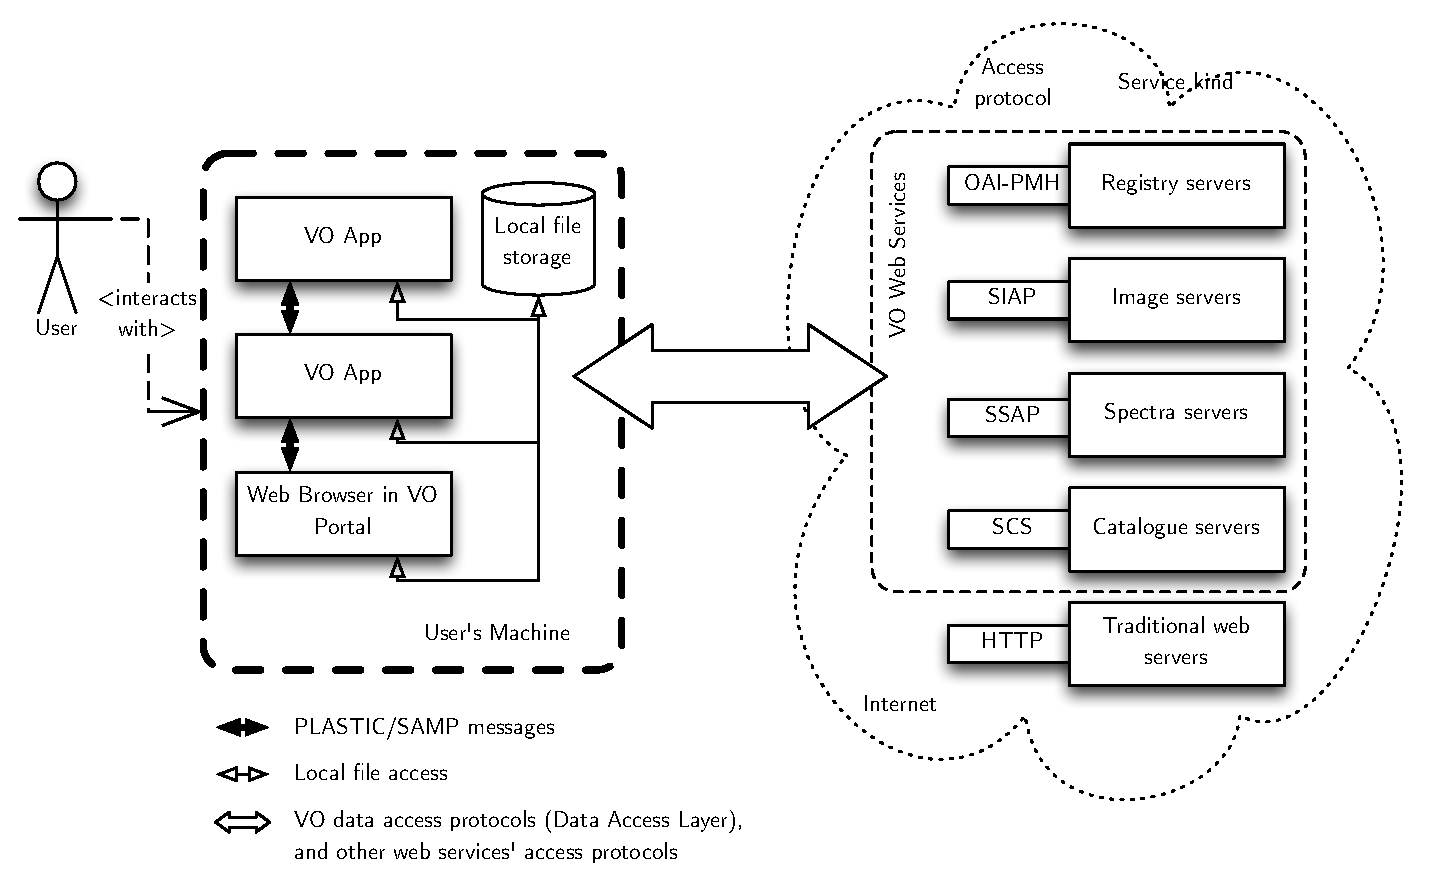
\includegraphics[width=\columnwidth]
				{fig/VOArchitectureFromUserPOV.pdf}
			\caption[User view of the VO]
			{
				High level VO architecture from the user's point of
				view. A user interacts with the VO via a variety of
				VO-aware, locally run applications, and accesses
				either locally archived files, or remote files,
				either via VO protocols or using a web browser to
				access a VO-enabled web portal. Users must only be
				aware of the different VO applications
				% \lourdesinline{VOapp no está definida}
				---VO app in the figure--- and/or VO portals of
				their interest, and that there exist interoperable
				image, spectra, and catalogue servers, transparently
				accessed from their toolset. They must also be
				aware that some VO applications can send messages
				and data between them, sending for instance data
				for analysis to some applications, and sending the
				received results to other applications for
				plotting. All the VO systems in the Internet
				---dotted cloud--- are indispensable for the
				operation of the VO, but are completely transparent
				to the user.
			}
			\label{fig:figUserPOV_VOArch}
		\end{figure}
		
		\invisiblenote{
			The VO architecture, as seen from the user point of
			view. Users can either access VO compatible files with
			VO-compliant tools, and use them more or less
			transparently in their workflow; or it could use a
			web-portal or a specific VO tool to explore VO datasets
			and retrieve those matching their criteria; or it could
			launch predefined VO-tasks on remote servers, which
			would bring VO compatible data back to the user.
		}
		
		 This can be better explained by means of an example.
		Imagine Alice is an astronomer who has already been
		introduced to the VO, and that she is searching for
		catalogues, images, and spectra on $\sigma$~Orionis, a
		star-forming region in the Orion belt.
		
		 She would fire up a tool such as the Aladin Sky Atlas, and
		use the search box to either specify the coordinates of the
		zone she is interested in, or would just write
		\texttt{sigma orionis}, and let Aladin query a name solver
		service, such as Sesame, to come up with the coordinates.
		
		 After having set the coordinates, Alice could set an
		angular radius for the search of interesting datasets,
		setting the separation for objects in the vicinity, or
		could just use the default radius. Aladin would ask
		different archives for both images and catalogues, laying
		catalogue data with coordinate information on top of the
		retrieved images, which can be composed from several bands.
		
		\begin{figure}[tbp]
			\centering
				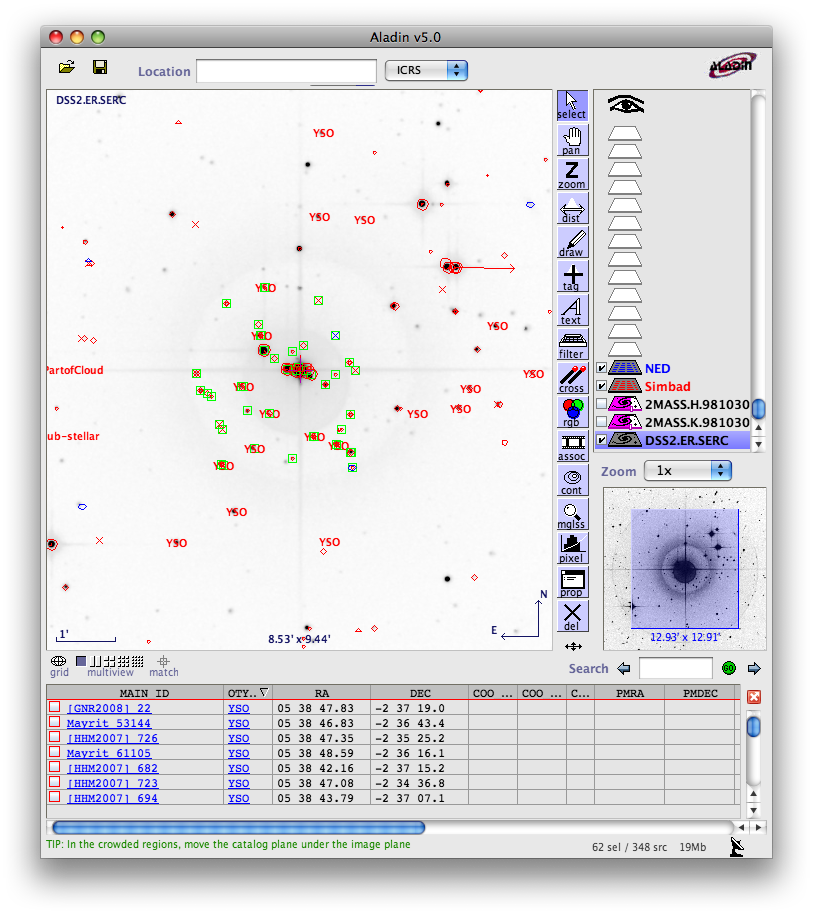
\includegraphics[width=\columnwidth]
				{fig/AladinSigmaOrionisDataSelection.png}
			\caption[Screenshot of the Aladin Sky Atlas]
			{
				Screenshot of the Aladin Sky Atlas: after having
				entered the coordinates for the $\sigma$~Orionis
				region in the search box on top of the window,
				Aladin has queried the Simbad and NED catalogues,
				together with the DSS2 server, and has overlaid
				catalogue objects on top of the DSS2 image.
				Besides, the astronomer has retrieved H-band and
				K-band images from the 2MASS survey, and has
				composed the three images by setting image
				transparencies. Besides, some data points of the
				central region have been selected, and are shown in
				the lower part of the window, sorted by the
				\texttt{OTYPE} (object type) column.
			}
			\label{fig:fig_AladinSigmaOrionisDataSelection}
		\end{figure}
		
		 She could, then, select catalogue data and send it to a
		table manipulation and plotting application, such as
		TOPCAT, to explore properties of the region.
		Figure~\ref{fig:fig_AladinSigmaOrionisDataSelection} shows
		what Alice's screen could look like while working with
		Aladin; figure~\ref{fig:fig_TopcatDatosSimbad}, instead,
		shows her computer's screen while using TOPCAT.
		
		\begin{figure}[tbp]
			\centering
				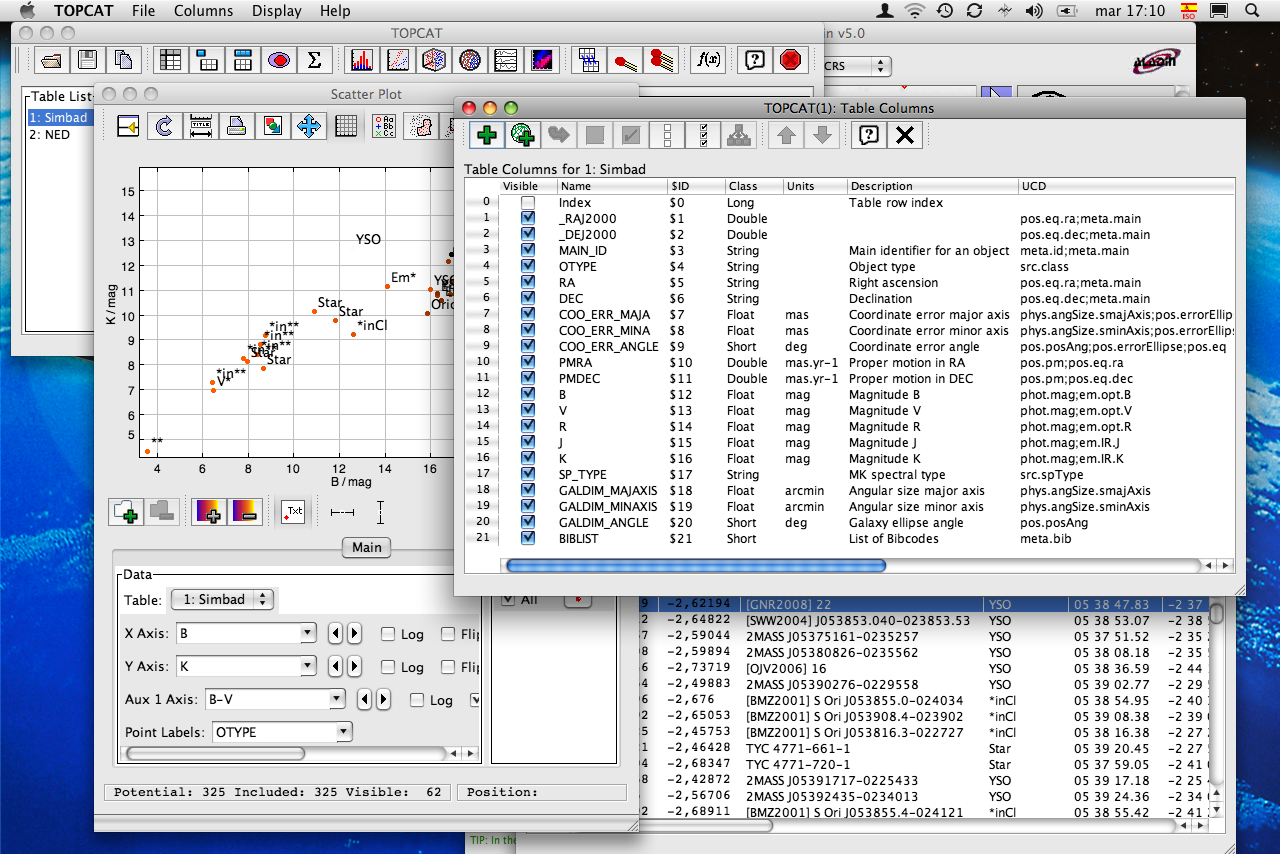
\includegraphics[width=\columnwidth]
				{fig/TopcatDatosSimbad.png}
			\caption[Screenshot of TOPCAT]
			{
				Screenshot of TOPCAT after having received two
				catalogues from Aladin via the PLASTIC VO messaging
				protocol. The windows shown, from left to right, and
				from top to bottom, are the main TOPCAT window,
				showing the two tables received from Aladin, which
				can be seen popping out to the right; a scatter
				plot of the $B$ magnitude against the $K$
				magnitude, using the $B-V$ color index for data
				point coloring, and with \texttt{OTYPE} as object
				label; the table column metadata, showing data
				types, units, description, and the UCD for of each
				column;
				% (the UCD is briefly described in 
				% section~\ref{sec:unified_content_descriptor_ucd})
				and the actual table data.
			}
			\label{fig:fig_TopcatDatosSimbad}
		\end{figure}
		
		 Another way to visualise the interaction of users with the
		VO is by means of a sequence diagram.
		Figure~\ref{fig:fig_VOClientSequenceDiagram} shows how
		users do not interact with VO services, they just interact
		with applications to provide object names, validate
		coordinates, and provide additional search criteria. VO
		applications are responsible of communicating with the
		different VO services (NameSolver, Registry, and data
		Services) on behalf of the user.
		
		% \lourdes{re-redactar párrafo anterior}
		
		\begin{figure}[tbp]
			\centering
				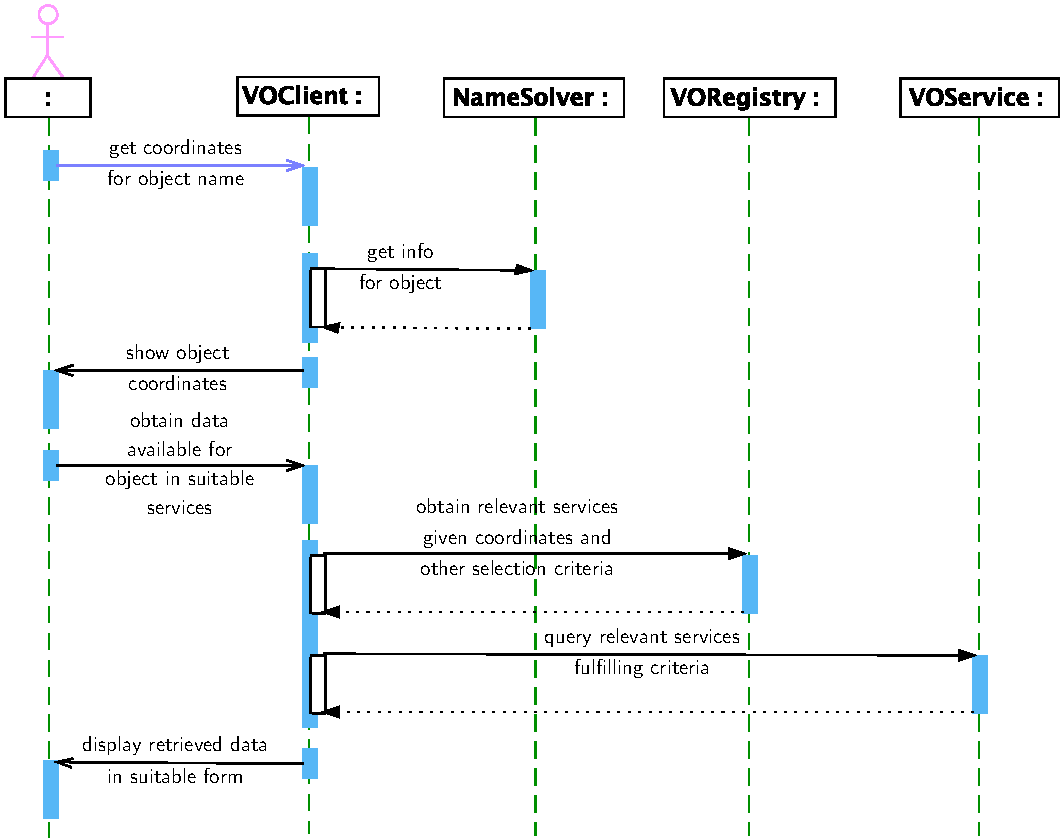
\includegraphics[width=\columnwidth]
				{fig/VOClientSequenceDiagram.pdf}
			\caption[Sequence diagram: User VO interaction]
			{
				UML sequence diagram of the user interaction with
				the VO. Users will typically use a VO client
				application to get information on particular
				objects of their interest. The user will first
				provide an object name, and the VO client will use
				an astronomical NameSolver to return celestial
				coordinates. With the coordinates, and some
				additional criteria, which might come from the
				application (a spectral analysis application will
				ask for spectral services; an image processing or
				manipulation package will ask for image services),
				or from additional criteria (wavelength, data
				quality, for instance) set by the user. Once the
				services are found, the application will query them
				(here only one such service query is shown), and
				the retrieved data will finally be provided to the
				user in a suitable form. This sequence diagram
				shows how user interaction with the VO is
				restricted to the use of VO application(s), while
				the orchestration of VO queries corresponds to the
				application.
			}
			\label{fig:fig_VOClientSequenceDiagram}
		\end{figure}
		
		For this user, the VO is just a set of software packages
		which can retrieve information from VO-enabled archives,
		and perform operations on such data, and on local data. The
		main differences with the way she used to work are:
		
		\begin{itemize}
			\item She uses spatial indexing on the data. Spatial
			selection goes first, archive, instrument, and
			wavelength selection are optionally performed in the
			next stage.
			
			 \item She does not have to know how many different
			archives might be of interest to her: within the VO,
			all archives containing data in the spatial zone of her
			interest will be queried. She can decide which data to
			finally download by looking at the archive metadata (to
			see if the wavelength range is appropriate or not, or
			who is responsible for the data quality), or at the
			particular dataset metadata (to learn specifics such as
			exposure time, observing configuration, and data
			quality flags).
			
			 \item She can combine the strengths of different tools
			by means of the VO messaging protocols.
			%\lourdesinline{presentar los local interop protocols.}
			
			 \item She can explore catalogues with higher
			confidence, because data columns are fully tagged with
			standard descriptors (UCDs, Unified Content
			Descriptors), which allow automated identification of
			those datasets.
		\end{itemize}
		
		In other words, she has transparent access to many archives
		not just from a single tool, but from any tool which is
		able to query the VO. In \emph{marketing} terms, any tool
		sporting a \emph{VO-compatible} badge.
		
		 However, if she wants to exploit the data she has just
		collected, for instance in order to perform cross-matching
		between sources, or to create different color diagrams, she
		needs to know how to find which data columns correspond to
		different astronomical or astrophysical concepts. In other
		words, she is concerned with data semantics.
		
		% However, the transparency to the user makes this view
		% miss the role of the VO as a standardisation force for
		% datasets, and also does not stress the power of common
		% semantics (the UCDs we have mentioned) between
		% archives, which allows for sensible comparison of
		% datasets.

	% subsection the_vo_from_the_point_of_view_of_the_user (end)

	\subsection{The VO from the application developer's point of view}
	% subsection % the_vo_for_the_application_developer (fold)
	\label{ssub:the_vo_for_the_application_developer}

		VO Developers view of the VO arises from what the VO offers
		for their applications. A VO-enabled application, be it
		brand new or upgraded, can be of two types: data centric or
		workflow centric. Some data centric applications can be
		scripted to be part of a workflow.
		
		 Data centric applications tend to be either data reduction
		applications or high level analysis applications which work
		on individual datasets at a time. For those applications,
		the VO is used for:
		
		\begin{description}
		
			\item[Finding out interesting datasets] That usually
		    means finding archives with data in the desired
		    wavelength range for certain positions of the sky.
			
			 \item[Retrieving candidate datasets] Candidate
		    datasets
			(be them images, spectra, data cubes)
			are downloaded
		    one by one, or as a package, to be individually
		    analysed in the local computer.
			
			 \item[Local processing] One by one processing of the
		    different datasets in order to obtain scientific grade
		    data products, such as chemical abundance, region
		    temperatures, ionisation states, stellar population
		    age, et cetera. Anything that is obtained from the
		    treatment of the light and the knowledge of the
		    physical process at hand.
		
		\end{description}

		 In this view of the VO, only a few benefits are added over
		the traditional astronomer's workflow, such as providing a
		single programmatic interface for all application to access
		all archives. That is, the VO provides a uniform data and
		metadata access, together with uniform data and metadata
		format to applications. Additionally, tools which implement
		VO messaging protocols allow the astronomer to use
		specialised tools for each task, while maintaining always
		the benefits of having each application connected to the
		VO.
		
		 On the other hand, workflow centric applications are
		applications which work with large datasets in large
		batches. For instance, from object types plus magnitudes in
		the 5 SDSS bands, photometric redshifts can be
		established\footnote{In fact, such processing is performed
		by the SDSS pipeline itself.}. Or data from different
		catalogues at different wavelengths can be cross-matched in
		order to find objects with particular properties which
		cannot be found through the original data of each
		individual dataset\footnote{If we have a catalogue of
		photometric magnitude measurements in $n$ bands per object,
		and combine it with $m$ additional photometric measurements
		in different bands, much more precise properties of those
		objects can be derived. As photometric redshift estimations
		make use of differences of magnitudes in as many bands as
		possible, their reliability depends on the number of pairs
		of magnitudes which can be built,
		$\begin{pmatrix}n\\2\end{pmatrix}$. But if we add $m$
		additional measurements, $\begin{pmatrix}n +
		m\\2\end{pmatrix}$ colours can be formed, and the relative
		increase in colours which can be formed is
		$\frac{(n+m)(n+m-1)}{n(n-1)}$, which is higher than the
		increase of just adding $m$ colours.}.
		
		 For those applications, the VO provides many more
		benefits: the access to archives is uniform, allowing
		simpler scripts, based around web services toolkits, to
		access all needed archives. Datasets are retrieved in a
		common format, and ready to analyse with XML tools.
		
		 Additionally, the VO community (in particular, the UK
		AstroGrid team\urlnote{http://www.astrogrid.org/}) has
		developed what is called the Common Execution Architecture
		(CEA)~\cite{Harrison:2005la}, a web-services wrapper for
		remote execution of tasks which can be called either with
		simple parameters (for instance, generating a synthetic
		spectrum from Kurucz models for stars with a given surface
		temperature, surface gravitational acceleration, and
		stellar type), or tasks which perform transformations on
		data in VOTable form (such as format transformations, or
		image generation from tabular data). As those tasks are
		exposed through a web services wrapper, users can get
		virtual data (data which was generated on the fly), or
		re-processed data, with the same kind of queries used for
		data retrieval.
		
		 In any case, the protocols that a VO application should
		implement are:

		\begin{description}
			\item[Object name queries] Many VO queries are
			spatially related, but for many sources there is a
			known source name, whose position is already well
			established. In those cases where the user wishes to
			query for other datasets near the source, being able to
			obtain the most recent coordinates, in different
			epochs, for a given object name, is one of the most
			important services in the VO. \invisiblenote{At the
			spatial level, it can be seen as similar to the
			internet Domain Name Solver services.} There are
			several services providing this target name to
			coordinates resolution, namely Sesame, the NASA
			Extragalactic Database (NED), and Simbad. However,
			Sesame is able to query both NED and Simbad, and is the
			primary service for name solving.
			
			 \newcommand{\cdssesamenote}[0]{ For instance, we can
			query Sesame about \emph{M31}, and we will learn that
			it is also known as \emph{Andromeda Nebula},
			\emph{Andromeda Galaxy}, or simply \emph{Andromeda}. In
			specific bands, it corresponds, for instance, with
			several strong infrared sources from the IRAS
			catalogue: \emph{IRAS~F00400+4059} and
			\emph{IRAS~00400+4059}. Sesame also returns object type
			information, and simply from querying Sesame we can
			learn that \emph{M31} is an active galaxy of
			\emph{LINER} type, with a morphology type of \emph{Sb}
			(a spiral galaxy without bars, with packed arms), and
			at a redshift (\emph{z}) of $-0.001004$, meaning that
			\emph{M31} is, in fact, blueshifted, getting nearer to
			the Milky Way at a rate of approximately $300
			\mathrm{km}/\mathrm{s}$.
			
			 The query which delivers all of this information, in
			XML format, is:
			
			 \noindent\url{\sesameurl}
		
			 See the CDS Developer's corner,
			\url{http://cdsweb.u-strasbg.fr/cdsws.gml}, for details
			on this and other services. }
			
			 An application querying Sesame must be able to parse
			not only the coordinates being provided, but also the
			different object aliases returned by the service, such
			as conventional names, coincidental sources at
			different wavelengths, morphology, redshift, and
			distance\footnote{\cdssesamenote}.
			
			 \item[Registry queries] Independently of the kind of
			VO services to be accessed, all applications must be
			able to query the VO Registry (or registries) so that
			they can look for specific services.
			
			 \item[Data access queries] Once we have coordinates to
			make our query (or queries), and the application (or
			the user) has selected entries in the registry that can
			provide useful datasets, the data access protocols
			relevant to the application (SCS, SIAP, SSAP, and in
			the future the TAP) have to be queried, and the
			returned data (in VOTABLE format) parsed.
			Appendix~\ref{cha:vo_protocols} is devoted to describe
			the interface to those services, and provides links to
			their complete specification.
			
			 \item[CEA services] If we want our application to take
			advantage of several remote VO services, such as those
			providing data transformation capabilities,
			mosaicing\footnote{Mosaicing is the non-trivial
			operation of overlaying several astronomical images,
			with embedded coordinates and resolution information,
			in order to provide a composition of the original
			images with a common resolution.}, signal processing,
			or many others running under the CEA, we must implement
			CEA services calls. The detailed description and
			specification of the CEA can be found
			in~\cite{Harrison:2005la}.
			
			 \item[Local messaging services] Optionally, the VO
			interoperability protocols for local data interchange
			and collaboration must be implemented. This allows a
			more modular development of VO tools, letting other
			applications to pre-process the data, and perform
			analysis in different ones.
		\end{description}

		In addition, as VO particular data formats are XML-based,
		XML manipulation toolkits are needed in order to build and
		interpret VO data, together with FITS processing libraries
		for applications which must have access to the actual data.

		\begin{figure}[tbhp]
			\centering
				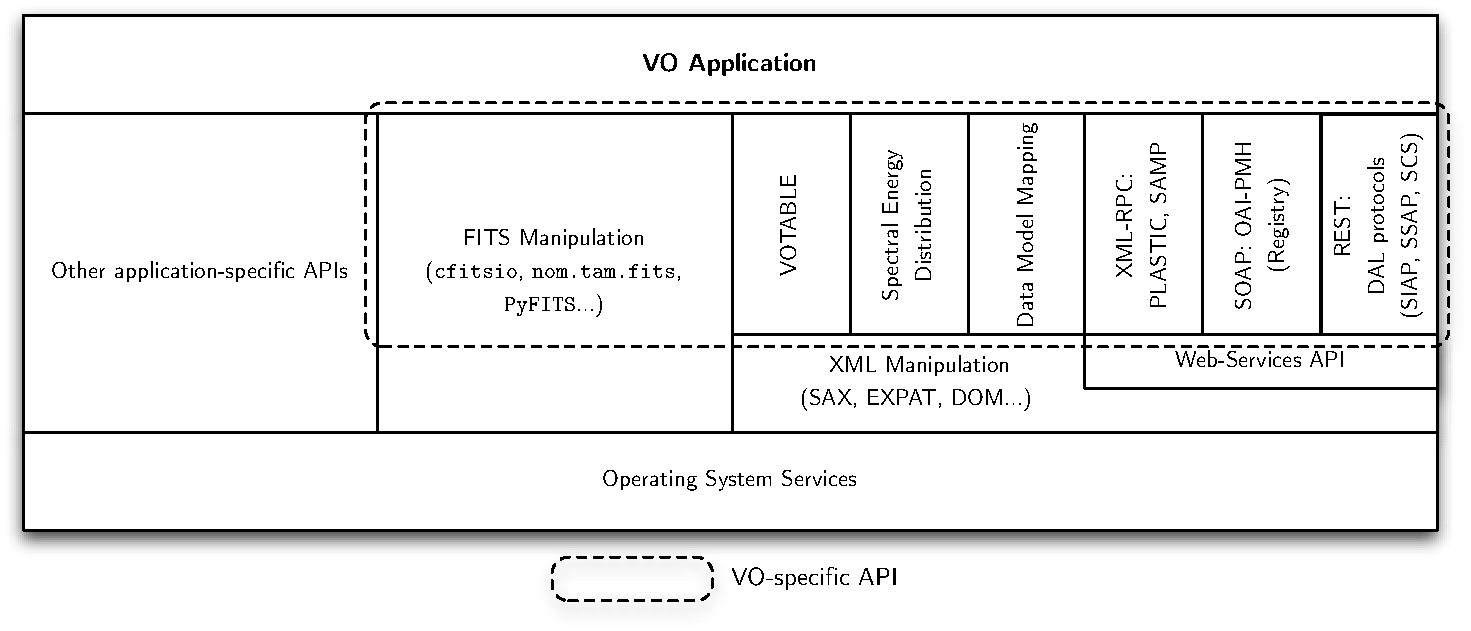
\includegraphics[width=\columnwidth]
				{fig/VOAPIStack.pdf}
			\caption[Application view of the VO]{
				The VO as seen from an application (developer)
				point of view. Applications trying to make use of
				the VO use web services technologies, such as REST
				queries, SOAP queries, or XML-RPC messages.
				Web-services calls require XML manipulation
				toolsets, which are also used to create, manipulate,
				and extract information from VOTables, the Spectral
				Energy Distribution XML representation, or
				different data model mappings. Finally, VOTABLEs
				can point to FITS files, and applications which
				manipulate scientific data must be able not only to
				read data from VOTables, but directly from FITS
				files. The VO specific part can be found in the
				dashed rounded rectangle, while the rest
				corresponds to either general APIs, or
				application-specific APIs.
			}
			\label{fig:fig_VOAPIStack}
		\end{figure}

		From the list above, it can be seen that the VO application
		interface for programmers (VO API) consists, then, of
		several more or less independent blocks, as shown in
		figure~\ref{fig:fig_VOAPIStack}.

		% We describe this programmatic interface to the VO with much
        % more detail in chapter~\ref{cha:voapi}.

		Let us imagine Bruce is an astronomical software developer.
		He has been creating astronomical software packages before
		the VO concept, and each time a new interesting archive
		appeared, he had to modify his application to perform the
		following tasks, every single time, without being able to
		reuse any code:

		\begin{description}
			\item[Service query] A new service query form, button,
			or other kind of user interactivity had to be added.
			
			 \item[Data access protocol] The query had to be
			implemented by encoding the service URL, service kind,
			and query parameters. Additionally, if the archive
			returns data in a particular format, a parser has to be
			implemented. % \lourdesinline{re-redactar}
			
			 \item[Data translation] The response data comes
			usually in a way that it is specific for the
			archive/service being queried, and must be translated
			into the data model of the querying application.
		\end{description}

		However, all steps above are common for all VO services
		providing the same kind of data (catalogues, images,
		spectra), with the addition of the Registry query step
		needed to find out all services providing that kind of
		data, which again has to be implemented only once.
		
		 It must be noticed that once the data are in the internal
		data model of the application, it does not matter which was
		the origin of a particular data set (except for documenting
		its provenance), and that is the way VO data can
		interoperate with non-VO data. An example of application
		mixing VO with non-VO data is Aladin: originally Aladin
		queried different non-VO services, and all VO-services were
		added as just one additional data source for Aladin.


	%	The VO as an Application Programming Interface. An
	%	application making use of the VO can see the different
	%	services it provides as a VO API. The different parts of
	%	the API are built on top of web-services client frameworks,
	%	and XML and FITS manipulation toolkits.
	%	
	%	 In fact, the AstroRuntime, from AstroGrid, provides such
	%	an API to the VO to allow XML-RPC enabled languages to
	%	programmatically access VO facilities, with an additional,
	%	more direct layer for Java applications through Java-RMI.


	% subsection % the_vo_for_the_application_developer (end)

	\subsection{The VO from the service developer's point of view}
	% the_vo_from_the_point_of_view_of_the_service_developer (fold)
	\label{ssub:the_vo_from_the_point_of_view_of_the_service_developer}

		For Bruce, then, the VO is technically rather simple
		(compared with the archive access and interface operations
		already in place in the archive): the services have to
		provide access to existing datasets through a web-services
		interface (most of the time, REST-ful services are used for
		the VO, except for VO Registry services, which use SOAP
		queries).
		
		 However, the hardest part for VO-services developers is
		the interfacing between the actual data being stored, and
		the VO data formats, which also include VO semantics. This
		is achieved by means of a systematic mapping between stored
		data and data models.
		
		 In particular a VO service needs to provide:

		\begin{description}
			\item[VO Service Endpoint(s)]
			% \lourdesinline{Explicar DAL, explicar endpoint}
			A service provider must provide one or more VO services
			(delivering images, spectra, or catalogue data). Each
			different service must provide an URL for accessing it,
			the endpoint. This URL is used to build VO queries by
			adding parameters to it. Different services, in the
			sense that the data they provide corresponds to a
			different scientific data product, need to provide
			different endpoints.
			
			 \item[DAL Parser and Query Mechanism] The service
			endpoint parameters have to be parsed, converted into a
			query for the internal database (or any other data
			access and filtering mechanism), and results obtained.
			In short, the service must comply with the interfaces
			described in appendix~\ref{cha:vo_protocols}.
			
			 \item[VOTable generation mechanism] Once the query has
			returned results, these must be returned into the
			VOTable format. This includes not only the building of
			the main tags, which can be considered a wrapper for a
			tabular result, but also the assignment of semantic
			attributes such as \texttt{ucd}s and \texttt{utype}s
			from data model mappings.
			
			 \item[Data Model Mapper] The VOTable generation
			mechanism, and the DAL Parser, need a mapping between
			the data stored in the database and the data model for
			the kind of observation being performed. This mapping
			is used for the filling of the already mentioned
			semantic attributes.
			
			 \item[CEA wrapper] A service which provides computing
			services in the VO environment has to comply with the
			CEA. A computing service which was not built for the VO
			can integrate into the CEA infrastructure by
			encapsulating it into a CEA intermediate service
			(wrapper).
			% \lourdesinline{Explicar wrapper.}
		\end{description}

		Other task to be eventually performed by the VO Service
		developer is the endpoint registration. Even when the VO
		Service can be used as long as its endpoint is known by any
		other tool (be it a simple command-line script, or a
		complete application), new services can only be discovered
		by tools if they are registered in a VO Registry.

	% subsection
	% the_vo_from_the_point_of_view_of_the_service_developer (end)

% section the_vo_from_the_point_of_view_of_different_actors (end)
	
	\section{Precedents to the VO} % (fold)
	\label{sec:precedents_to_the_vo}
		
		Due to the purely scientific, non-commercial nature of astrophysical
data, public access to them has always been the norm. With the
connection of most educational and research institutions to the
Internet, the first primitive online archives were born. One of the
first was that of the International Ultraviolet Explorer (IUE), which
was made available to the public in 1985. As the World Wide Web did not
exist yet at that time, astronomers had to login to remote servers from
which the data were downloaded through the File Transfer Protocol
(FTP).

Apart from the data from observations themselves, articles and other
publications on astronomical objects were also of great value, and
during the \emph{Astronomy from large databases}
conference~\cite{1988afld.book.....M}, held in 1987, a proposal was
made for the design and operation of a system to compile all
astronomical publications, the SAO/NASA Astrophysics Data System (ADS).
A prototype was built in 1990, with the system being released to the
public in early 1993~\cite{1993ASPC...52..132K}. The system was made
possible thanks to the collaboration of the publishing journals.

Simultaneously, systems like the Simbad Astronomical
Database\urlnote{http://simbad.u-strasbg.fr/simbad/}~\cite{
2000A&AS..143....9W} (an online database hosted by the Centre de Donées
Astronomiques de Strasbourg, CDS), or the NASA/IPAC Extragalactic
Database\urlnote{http://nedwww.ipac.caltech.edu/}~\cite{
1992ASPC...25...47M} (NED) contained data with diverse information on
observed astrophysical objects, which were compiled, maintained and
published online by the respective large scale astronomical data
centres.

\newcommand{\adsbibcodeurl}[0]
{http://doc.adsabs.harvard.edu/abs_doc/help_pages/bibcodes.html}
As all of these initiative had grown independently, the were developed
with different considerations in mind, and were not coordinated.
However, the possibility of joining publications available at the ADS,
and the Simbad/NED databases, allowed astronomers to have access to
publications on the objects of their interest, or to access more data
in those databases from the corresponding literature. The joint
ADS/NED/Simbad effort was called URANIA~\cite{1996AAS...189.0603B}, and
is one of the first joint initiatives for data service interoperability
in astronomy. The main product of that agreement is the
\emph{bibcode}\urlnote{\adsbibcodeurl}, a unique identifier of
publications which encodes details on the publication date, publication
kind, and/or journal, and author\footnote{When astronomers upload data related to a particular publication to the NED or Simbad services, or that data is gathered from the publication, the bibcode allows the cross-identification of sources and publications.}.

\newcommand{\vizierurl}[0]
{http://webviz.u-strasbg.fr/viz-bin/VizieR}
Outside the URANIA project, the
INES\urlnote{http://sdc.laeff.inta.es/ines/} (IUE Newly Extracted
Spectra)~\cite{1999A&AS..139..183R} archive, holding reprocessed IUE
observations, represents the first instance of interoperability between
two completely different astrophysical services: one holding spectral
information (INES), the other keeping bibliographical references (ADS).
It was possible to access the information available in ADS for a
particular object from the INES archive, and from the ADS the INES
spectra used for a particular article could be accessed. Other service
linked to the ADS through bibcodes is the VizieR\urlnote{\vizierurl}
service for Astronomical Catalogues~\cite{2000A&AS..143...23O}.

Another important milestone in the development of online, interoperable
archives was the NASA multi-mission archive initiative, which tried to
provide a common archival infrastructure across different space-borne
missions. Three portals were finally created:
MAST\urlnote{http://archive.stsci.edu/} (Multi-mission Archive at Space
Telescope)~\cite{1999AAS...194.8302I}, mainly for optical-ultraviolet
observations\footnote{VLA FIRST images are also available through
MAST.}; IRSA\urlnote{http://irsa.ipac.caltech.edu/} (InfraRed Science
Archive)~\cite{2000AAS...19711610B}, for the infrared; and
HEASARC\urlnote{http://heasarc.gsfc.nasa.gov/} (High Energy
Astrophysics Science Archive Research
Center)~\cite{1994BAAS...26..995R} for high-energy (X-rays, gamma rays)
astrophysical observations. These portals allowed for the first time a
unified view of data from widely different provenance under the same
query interface. MAST also provided some applications for data
visualisation across mission, such as the
COPLOT\urlnote{http://archive.stsci.edu/mast_coplot.html} tool.
However, data products from each mission were, still, quite different.

Finally, regarding the use of applications in order to combine and
manipulate data from different services, one of the first examples
prior to the VO development is the Aladin Sky Atlas. Initially, Aladin
was only able to access CDS-based catalogues and images, which were
accessed through custom built, Aladin-specific protocols. However,
Aladin helped in making developers and astronomers realise that any
other system which shared the data access and data description
protocols would allow either to improve Aladin, by allowing it to
access more datasets, or more easily recreate Aladin-like functionality, without the need of being a data and service provider.
		
		\invisiblenote
		{The VO infrastructure has taken advantage of already in
		place systems. The main precedents are:
		
		\begin{description}
			\item[The NASA/IPAC Extragalactic Database] The
			NED\urlnote{http://nedwww.ipac.caltech.edu/}~\cite{
			1992ASPC...25...47M} (service acronym), provides online
			all different catalogues of extragalactic objects ever
			published in astronomy. It allows users to perform
			\emph{conesearchs} for data centred on a particular
			position, and below a certain angular distance, and the
			results provide the main object positional properties:
			sky coordinates, distance, relative velocity, object
			type, morphological classification, et cetera; it also
			provides many other observational parameters, such as
			galactic extinction, absolute magnitudes, et cetera.
			
			 \item[The Simbad Astronomical Database]
			Simbad\urlnote{http://simbad.u-strasbg.fr/simbad/}~\cite{
			2000A&AS..143....9W} is an online database hosted by
			the Centre de Donées Astronomiques de Strasbourg (CDS),
			also providing data on different objects outside of our
			solar system, and thus includes galactic objects. The
			two databases have a non-empty intersection, but none
			is a subset of the other.
			
			\newcommand{\vizierurl}[0]
			{http://webviz.u-strasbg.fr/viz-bin/VizieR}
			\item[The
			VizieR service for Astronomical Catalogues]
			VizieR\urlnote{\vizierurl}~\cite{2000A&AS..143...23O}
			is a compilation of all published astronomical
			catalogues, classified by waveband coverage, space
			mission if applicable, and/or astrophysical subject.
			Many astrophysical journals automatically make
			available in VizieR positional tables in published
			articles, and the data is linked to the publication via
			the \emph{bibcode} of the Astrophysics Data System
			(ADS).
			
			\newcommand{\adsbibcodeurl}[0]
	   {http://doc.adsabs.harvard.edu/abs_doc/help_pages/bibcodes.html}
			\item[The SAO/NASA Astrophysics Data System] The
			ADS\urlnote{http://www.adsabs.harvard.edu/}~\cite{
			2000A&AS..143...41K} is an online da\-ta\-base
			containing all bibliographic entries in the fields of
			Physics and Astrophysics. Entries are proposed by
			different journal and book publishers, but are also
			collected from online e-print archives such as the
			arXiv\urlnote{http://arXiv.org/}. Publications are
			uniquely identified by a structured code, the
			\emph{bibcode}\urlnote{\adsbibcodeurl}, which contains
			details on the publication date, publication kind,
			and/or journal, and enough data for unique
			identification or journal articles. The entries are
			linked with online versions of the articles, if
			available, and can be searched by author, words in
			title or abstract, publication dates, et cetera. VizieR
			catalogue entries are also considered publications by
			the ADS, with their own \emph{bibcode}.
		\end{description}
	
		These facilities have been federated and linked by means of
		the \emph{bibcode}, which allows for the retrieval of
		publications on any object in Simbad or NED, or for the
		objects whose data is found in VizieR.
		
		 And many observatories, specially space-borne ones, have
		had online archives from little time after the opening of
		the Internet and the World Wide Web.
		
		 However, all of these services have their own, completely
		different form-based interfaces, and even when they have
		started to provide cleaner web-services interfaces, users
		need to support different query protocols for each service,
		until the VO provided service unification and
		interoperability templates.
		}
	% section precedents_to_the_vo (end)

	\section{Comparable activities in other disciplines} % (fold)
	\label{sec:comparable_activities_in_other_disciplines}
	
	We will conclude our introduction of the VO with a selection of
	other e-science activities which are similar in scope to the
	Virtual Observatory, but belong to different scientific fields,
	or have a different technology base: the data storage support
	of data grids, Geographical Information Systems, and the
	Bioinformatics Harvester.
	
	\subsection{Data grids} % (fold)
	\label{sub:data_grids}
	
		In e-Science talks, grid technologies tend to come up first
		and forefront. It is very usual for national e-Science
		initiatives in European countries to be represented by the
		National Grid Initiatives, as if e-Science could only be
		performed via grid technologies. It is true that grid
		middleware provides tools to implement much of VO core
		functionality, but at the cost of a greater complexity, and
		greater demands on client systems.
		
		 The definition of grid computing by Ian Foster as \emph{a
		hardware and software infrastructure that provides
		dependable, consistent, pervasive, and inexpensive access to
		high-end computational
		capabilities}~\cite{1999gbnc.book.....F} is just one part
		of the Virtual Observatory.
		
		 But computation is just a fraction of the VO. In fact, the
		VO can be more closely identified with a \emph{data
		grid}~\cite{Chervenak:2001rr}: an extension of the grid
		protocols in order to create a standard for distributed
		data storage, data identification, and metadata management
		which can integrate archives from different disciplines.
		
		 In the VO, the \emph{data grid} exists via the data access
		protocols, and the standardisation of metadata. A version
		of the VO can exist implemented on top of grid protocols,
		but web-services technology was chosen instead in order to
		minimise the cost of entry for participant
		institutions/research groups: web-services technology is
		easier to implement and deploy, both for servers and
		specially for clients, and it was very important to be able
		to have a productive VO that could engage the community.
		
		 In the future, however, the VO can move more towards a
		grid technology foundation, when the computing needs
		overcome the data needs, and the VO metadata standards are
		complete. In the meantime, VO protocols are as technology
		agnostic as possible. For instance, the IVOA is working in
		a distributed file system for VO tools, reminiscent of grid
		data storage pools, with VO specific metadata and
		implementation independent (it can use WebDAV, NFS,
		GridFTP, or any other supporting protocol), called
		VOSpace~\cite{2008vospcivoav1013G}.
	% subsection data_grids (end)
	
	\subsection{Geographical Information Systems} % (fold)
	\label{sub:geographical_information_systems}
	
		There are many similarities between the VO and 
		Geographical Information Systems (GIS):
	
		\begin{description}
			\item[Coordinate system based] Both for GIS and the VO,
			coordinates are one of the main indices on data.
			Finding data nearby a particular coordinate is also a
			common feature, and the retrieval of nearby candidates
			cannot be based on floating point differences, as it
			would become computationally costly. The solution for
			fast operation of coordinate-based data retrieval is
			the hierarchical partitioning of the search space
			using, for instance, techniques such as the
			Hierarchical Triangular Mesh~\cite{2001misk.conf..631K}
			or the Quad Tree Cube~\cite{2006ASPC..351..735K}.
			
			 \item[Object to coordinates resolution] Also common to
			both problem domains is the need to obtain coordinates
			for a particular object whose only known property is
			the name. In astronomy such needs are typically handled
			by the Simbad or NED services, while different GIS
			systems will use different local or remote databases
			for obtaining the coordinates.
			
			 \item[Use of metadata] GIS objects are primarily
			graphs\footnote{In the mathematical sense: a
			set of directed connections between sets of nodes.}
			with geographical coordinates attached to both
			connections and nodes. But those curves represent
			roads, buildings, water and gas distribution pipes,
			agricultural plantations, et cetera, and each object
			kind has its own set of metadata, in the same way VO
			data uses metadata to establish object kind, and
			information kind.
		\end{description} 
	
		The main difference between the VO and GIS systems is that
		for the VO there is a strong standardisation force
		mandating which data formats to use, and there is usually
		no restriction in data usage\footnote{After all,
		astrophysical data tend not to be of immediate value for
		entrepreneurial use.}, and interoperation and networking is
		a key concept in system design, while it is not so for GIS.
		
		 However, some GIS systems such as Google
		Earth\urlnote{http://earth.google.com/} have started to
		show the potential of having a common geographical
		description format combined with the distributed dataset
		creation and distribution: GIS data, both images and object
		catalogues with metadata can be updated on the data server,
		and all clients access updated data from then on.
		
		 It is remarkable in this context that Google Earth has
		evolved to include Google Sky, which demonstrates the
		similar nature of GIS and VO systems when the distributed,
		interoperable data access is taken into account.
	
	% subsection geographical_information_systems (end)
		
	\subsection{Bioinformatic Harvester} % (fold)
	\label{sub:genbank}
	
		The Bioinformatic
		Harvester\urlnote{http://harvester.fzk.de/harvester/}
		(BioH) is a bioinformatic meta search engine at KIT
		Karlsruhe Institute of Technology for genes and
		protein-associated information. It queries data from more
		than 35 bioinformatic sites, which allows for searches in
		the genome and proteins of several animals of the most
		important sequenced animals ---among them humans, rats, or
		the drosophila (fruit fly)--- or on the complete
		collection.
		
		 The similarities with the VO lie in the distributed nature
		of the integrated systems, but the similarities end there:
		
		\begin{itemize}
			\item the BioH does not use a unified, standardised
			protocol for harvesting the data available in the
			different resources; instead, it uses a custom built
			harvesting engine for each collection.
			
			 \item there is only one entry point to the Harvester,
			and there is no public service access entry point for
			external applications.
		\end{itemize}
		
		 We can see the BioH as bioinformatic equivalent of the
		state of affairs in astronomy prior to the VO: similar to
		the joint ADS and VizieR systems.
	
	%GenBank\urlnote{http://www.ncbi.nlm.nih.gov/Genbank/} is the
	%NIH genetic sequence database, an annotated collection of all
	%publicly available DNA sequences. It contains approximately 86
	%thousand million bases in almost 83 million sequence records in
	%the traditional GenBank divisions, while more than 100 thousand
	%million bases on 27 million sequence records are held in the
	%WGS (large genome sequencing projects) division.
	%
	% The main connection point with the VO is that it is a public
	%driven effort which is central to a particular community
	%(astronomers for the VO, geneticists for the GenBank). However,
	%the GenBank is quite opposite to the VO in many aspects:
	
	
	% subsection genbank (end)
	
	% section comparable_activities_in_other_disciplines (end)
	
	\section{Status of the VO} % (fold)
	\label{sec:status_of_the_vo}
		
		As we have said, the VO initiatives were conceived around
		2000, and first prototypes built around 2002. Even
		when some parts of the VO are still being built ---being
		the IVOA Table Access Protocol (TAP) one of the salient
		examples of \emph{in progress} infrastructure---, and
		some of them being subject to changes (the Image and
		Spectral Access protocols are being reviewed), many of
		the tools are mature enough as to produce scientific
		results beyond what was possible prior to the VO.
		
		In particular, the first paper on VO-enabled science
		was published by Paolo Padovani in
		2004~\cite{2004AaA...424..545P}, and reported on the
		discovery of faint, obscured quasars with Virtual
		Observatory tools. However, more than half of all
		VO-enabled scientific
		papers\urlnote{http://www.euro-vo.org/pub/fc/papers.html}
		have been published since 2007 and onwards, while
		more than 90 percent of papers were published after 2006,
		which indicates a shift toward the maturity of the VO
		infrastructure and tools.
		
		\newcommand{\votableoneohurl}
	{http://www.ivoa.net/Documents/PR/VOTable/VOTable-20031017.html}
		\newcommand{\siaoneohwdurl}
		{http://www.ivoa.net/Documents/cover/SIA-20040524.html}
		\newcommand{\ssaoneoneprurl}
		{http://www.ivoa.net/Documents/cover/SSA-20070604.html}
		This can be easily correlated with the development of IVOA
		standards: the first IVOA Recommendation of the VOTable
		dates from October 2003\urlnote{\votableoneohurl}; the
		first agreed working draft for the Simple Image Access
		protocol was published in 2004\urlnote{\siaoneohwdurl}; the
		first ConeSearch services were available soon after that,
		with the ConeSearch specification being published in 2006;
		the Simple Spectral Access protocol, finally, was only
		proposed as a recommendation in
		2007\urlnote{\ssaoneoneprurl}, and prior to that only
		prototype spectral services, reusing the Image Access
		protocol, existed.
		
		It is interesting to mention that one of the national
		VO initiatives pushing the most towards the development of
		VO scientific tools is the SVO, as more than half of VO
		papers have been published by SVO-related groups.
		
		%\todo{\textbf{Enrique}, ¿puedes confirmar esto?}
		
		In the IVOA InterOp meeting of Baltimore (October, 2008),
		the former IVOA Chair, Dave de Young, proclaimed the VO
		had entered the operational status, where all infrastructure
		is mostly put into place, and science is routinely possible
		with existing tools.
		
		In this thesis, we will try to help in bringing radio
		astronomical archives and tools to that operational stage.
		
	% section status_of_the_vo (end)
	
	
	
%	\section{Current problems of the VO} % (fold)
%	\label{sec:current_problems_of_the_vo}
%
%		Even now that the IVOA and the VO have been declared as
%		reaching operational status at the IVOA Fall InterOp of
%		Baltimore in 2008, many issues are still open,
%		or are of further concern:
%		
%		\begin{description}
%			\item[Registries contain lots of useless entries] The
%			minimum mandatory metadata for a resource entry is mandated
%			by the Dublin Core metadata, but it is not enough for many
%			applications. In addition, some registry entries for VO
%			services are outdated, and link to non-existing servers.
%			Automated checks of the validity of registry entries are
%			useful, but manual purging of non-useful entries should
%			decrease the number of entries, and increase the usefulness
%			of the registry as a whole. In any case, users and/or VO
%			tool developers need to take this into account.
%			
%			\item[label] description
%			\item[Many tools have not made the transition the VO]
%			Many astronomical tools
%		\end{description}
%
%	% section current_problems_of_the_vo (end)

% chapter intro_vo (end)
	
	% %Rule for 71 characters
%2345678901234567890123456789012345678901234567890123456789012345678901
\chapter{Programmatic Interface to the VO} % (fold)
\label{cha:voapi}

\begin{verbatim}
	Intro
		Typical use of APIs
		The APIs of the VO
			Name solving
			Registry query
			Data Access
			Data Manipulation
	The VO API by kind of activity
		Sky and Time indexing
			Space and Time Coordinates
		Name Solving
			Name resolvers: galactic and extragalactic
		Registry
			Resource finding
			URI resolving
		Data Access Layer
			Access to catalogues
			Access to images
			Access to spectra
		Data Manipulation
			Table manipulation
				STILTS
			XML manipulation
				Typical XML APIs
		Remote execution and grid services
		Local interoperability
		Plotting
			TOPCAT
			VOPlot
	The VO API by kind of access type
		SOAP Interfaces
		REST Interfaces
		XML-RPC Interfaces
		Libraries
	Future VO APIs by kind and access type
\end{verbatim}

The Virtual Observatory is a software 

% chapter voapi (end) 
	
	% part intro_vo (end)
	
	% part VO data models (fold)
	\part[Radio astronomical archives in the VO]
	{Radio astronomical archives in the VO}
	\label{partRadioDataModelling}
	
	% % chapter specific_characteristics_or_radio_signals (fold)
\chapter{Radio astronomical observations}
\label{introradiospecifics}

This chapter attempts to summarise the main concepts in radio
astronomical observations relevant to astronomical data archival and
retrieval. For an excellent overview of radio astronomy, used as a source
for this thesis, the reader might consult Rohlfs and Wilson's
\emph{Tools of radio astronomy}~\cite{2004tra..book.....R}.

Radio telescopes detect electromagnetic (EM) radiation generated all
around the universe. The first astronomical radio source ever detected
was the nucleus of our own galaxy, when Karl Jansky received an
extraterrestrial signal in his array of dipole
antennas~\cite{Jansky:1933db, Jansky:1935lq}.

The mechanisms for generating radio EM radiation involve the deceleration
of electrons, whose energy losses are radiated away. There are two main
mechanisms for such radiation: slow electrons (moving at a small fraction
of the speed of light, $c$, but can be moving at hundreds of kilometres
per second) interacting with hot clouds of ionised gas, or relativistic
electrons accelerated by some kind of large scale explosion and moving
within a magnetic field. The first kind of emission is normally called
\emph{thermal emission}, as it is mainly dominated by the thermal
properties of the gas, and the second one is called \emph{synchrotron
emission} or radiation, as the emission mechanism is dominated by strong
circular acceleration.

The range for radio waves can be seen in
table~\ref{tab:RadioWavelenghts}.

\todo{Build \texttt{tab:RadioWavelenghts} table, including the name of
radio bands, and their typical extent.}

\section{Angular resolution} % (fold)
\label{sec:angular_resolution}

Single-dish radio astronomical telescopes receive all incoming radiation
within a beam whose angular resolution depends on the wavelength of the
radiation, and on the diameter of the telescope.

\todo{Look up \emph{Tools of radio astronomy}, \emph{The invisible
universe}, y el TIT de Vicent para la parte de la descripción del
patrón del haz y demás. Repasar curso de radio astronomía de IRAM.}



% section angular_resolution (end)

\section{Observing modes} % (fold)
\label{sub:observing_modes}

\todo{Coger tesis de Itziar y explicar observaciones espectroscópicas.
Buscar también observaciones de contínuo. Aprovechar también manual de
HIFI, y repasar manual de IRAM.}

\todo{
	\begin{itemize}
		\item single-dish vs. interferometry
		\item spectra
		\item continuum observations
		\item maps
		\item OTF
	\end{itemize}
}

% section observing_modes (end)

\section{Data reduction} % (fold)
\label{sub:data_reduction}

\todo{Specify data reduction steps in connection with the
      observations that have to be combined.}

% section data_reduction (end)

\section{Data products} % (fold)
\label{sub:data_products}

\begin{itemize}
	\item single-dish continuum
	\item single-dish spectra
	\item single-dish maps
	\item OTF data-cubes
	\item interferometry data-cubes
\end{itemize}

\section{Radio astronomical units} % (fold)
\label{sec:radio_astronomical_units}

% section radio_astronomical_units (end)

% section data_products (end)

% chapter specific_characteristics_or_radio_signals (end)

	%2345678901234567890123456789012345678901234567890123456789012345678901

\chapter{Introduction} % (fold)
\label{cha:introduction}
	
	Due to the more abstract nature of radio astronomical
	observations, there are less astronomers and observatories
	providing radio astronomical data when compared to those
	working on the visible part of the spectrum. However, as
	multi-wavelength studies become more and more commonplace in
	astrophysics, and are essential for studies such as the one
	being carried out within the AMIGA group, the capability of
	having access to radio astronomical data becomes of the utmost
	importance.
	
	 There are few radio astronomical observatories with proper
	archives (most of them provide just logbooks, or observation
	registries), so providing VO-compatible radio
	astronomical archives is a valuable contribution to the
	community both because of the availability of the archive
	itself, and
	the bonus possibility of using VO-tools to access it.
	
	 For existing archives, the data model of the archive itself
	does not usually match the data model of the VO, mainly due to
	the difference in scope: archive data models reflect the data
	origin, and are built to answer the queries of engineers,
	commissioning scientists and scientists; VO data models, on the
	other hand, are built to describe observations so that the
	description is enough for astronomers, or computer queries, to
	assess the usefulness of a particular piece of data.
	
	 For a new archive, however, the internal archive data model
	can be built by mirroring VO data models, while adding non-VO
	information so that all needs can be covered.
	

	 In this part, we will describe the RADAMS, a data model for
	single-dish radio astronomical archives reflecting existing
	IVOA data models, but which at the same time provides
	definitions and proposals for modelling additional
	observational aspects. We will use this data model for the
	building of the IRAM 30m and DSS-63 archives, which will be
	shown  in
	Part~\ref{prt:thesis_applications}.
	
	 In addition, some parts
	of the RADAMS will be used in the development of the MOVOIR, 
	a modular VO interface and API to the VO, which will be
	described in Part~\ref{prt:legacyTools}.
	
	%  We will see both approaches when describing the archives for
	% the DSS-63 and IRAM 30m antennas. For the former, no archiving
	% infrastructure existed in the first place, and thus the RADAMS
	% was built with the intent of being used as a blueprint for
	% this archive development. For the latter, earlier archive
	% organisation attempts had been made, specially for pooled
	% observations\footnote{Pooled observations are observations which
	% are scheduled from a pool of available observations projects
	% regarding project priority, weather conditions, availability of 
	% sources, and  availability of allocated time for the project.
	% Pooled observations enhance the project completion rate and
	% scientific return for an observatory, as backup programas
	% exist for non-optimal weather conditions.}. In this case, the
	% RADAMS is built as a layer on top of the existing, instrument
	% specific data model.
	
	We will start by introducing which are the existing IVOA data
	models in chapter~\ref{cha:data_modelling_in_the_vo}, and then
	we will evaluate parts of those models to create the RADAMS
	(Radio Astronomical DAta Model for Single-dish observations) in
	chapter~\ref{cha:radams}. Chapter~\ref{cha:radamscharobs}
	explains how the RADAMS can be used to characterise
	astronomical observations, and the following chapters explore
	in detail which are the missing parts in IVOA data models which
	are needed for the RADAMS: Curation, Packaging and Policy are
	specified in
	chapter~\ref{cha:radams_curation_packaging_and_policy}, while
	data provenance in e-science is reviewed in
	chapter~\ref{cha:data_provenance_in_the_vo}, and the lessons
	learned applied to RADAMS' Provenance in
	chapter~\ref{cha:radams_data_provenance}.
	
% chapter introduction (end)
	\chapter{Data modelling in the VO} % (fold)
\label{cha:data_modelling_in_the_vo}

% - VO seeks common services and data interoperability
% 
% - Common services must satisfy typical astronomy tasks, plus new data
%   mining needs
% 
% - Common services, as shown before
%   - Images
%   - Spectra
%   - Multi-dimensional datasets (to be defined, extending one or other
%     previous services)
% 
% - Data interoperability, needs a MODEL of astronomical data and
%   operations, so that data and applications can adhere to it.
	
	\invisiblenote{
		mod•el |ˈmädl| 
		noun 
		• (in sculpture) a figure or object made in clay or wax, to be reproduced in 
		another more durable material. 
		2 a system or thing used as an example to follow or imitate : the law became a model for 
		dozens of laws banning non-degradable plastic products | [as adjective ] a model farm. 
		• a simplified description, especially a mathematical one, of a system or process, to 
		assist calculations and predictions : a statistical model used for predicting the survival rates 
		of endangered species. 
		4 a particular design or version of a product : trading your car in for a newer model.
	}
	
	The interoperability of tools and archives in the VO is only
	achievable by standardising the way datasets are accessed, and
	how the scientific data they contain is described. The first
	part is solved by means of standard access protocols, while the
	latter needs the development of suitable data models.
	
	 A data model can be defined as a complete description of the
	set of entities needed for information storage in a particular
	field, which specifies both the data being stored, and the
	relationships between them.
	
	 In this way, it can also be seen as the framework in which
	questions about the data (and metadata) ca be posed: only
	questions which can be answered regarding the information AND
	relationships encoded in the data model can be answered within
	the VO framework. And considered this way, a uniform,
	interoperable observation data model can be mapped into
	a uniform set of questions which can be answered within the VO.
	
	 Two main classes of data models are typically considered:
	
	\begin{description}
		\item[Domain data models] These are high-level descriptions
		of the entities to be taken into account in order to fully
		implement a data model. Particular attributes of the data
		entities involved are not set, except for those needed for
		establishing the relationship between entities.
		
		\item[Implementation model] Implementation-dependent
		description of the particular entities and attributes to be
		actually stored.
	\end{description}
	
	 VO data models need to be a mixture of the model types above:
	for the data models to be used across observations with
	different instruments, and with different scientific objectives
	in mind, a high-level description is needed. In addition, VO
	data models affect how data from observatories' archives are
	exposed through VO services, as the way such
	data are stored by the archive might differ from the IVOA
	standards. 
	However, there are
	particular attributes that need a precise description in order
	for the model to be useful, and to be able to implement it,
	so VO data models need to fix the kind of metadata they
	support.
	
	 Within the VO, data models apply not only directly to the
	scientific data, but to the metadata describing them. As the
	way to structure information depends on the application domain,
	VO data models describe astronomical datasets in a way that is
	as instrument independent as possible, to ensure that the same
	description can be used for data with different origins.
	Users must also be able to query those data models to be able
	to find datasets which comply with certain properties.
	
	\section{Elements of a data model} % (fold)
	\label{sec:data_model_elements}
	
		When defining a VO data model, we have to specify:
	
		\begin{description}
			\item[Entities] Being the data model building blocks,
			they group related attributes within a data model. They
			can be mapped to Classes in Object-Oriented Programming
			(OOP), or Elements in XML.
			
			 \item[Fields] They are the actual data elements of the
			model. They map to Attributes in OOP, and they can be
			mapped to Attributes or to Elements without children in
			XML.
			
			 \item[Relationships] The different entities and fields
			have hierarchical or relational relationships: an
			observation project has projected observations, and
			all entities which share a common project ID are
			related, for instance. For the data model to be
			uniquely defined those relationships must be made
			explicit.
			
			 \item[Cardinalities] The number of object instances
			allowed as part of a relationship. It is specified as
			a range of valid number of entities.
			For instance, an
			observation can be related to any number of data files,
			but it needs to be related at least with one, meaning
			that the cardinality of the Observation to Data files
			relationship would be specified as 1..*. For objects
			which can appear any number of times, including none,
			the cardinality is expressed as 0..*. Objects which are
			optional, but if present can appear just once have their 
			cardinality expressed as 0..1, and so on.
			
			 \item[Data types] For computers to be able to
			correctly interpret a data stream a Data type needs to
			be specified. For instance, object IDs could be
			Integers, but they are normally textual, so String data
			must be used. We could consider the restrictions which
			can be defined for complex data types in XML as part of
			the data typing.
			
			 \item[Units] No physical quantity can be specified
			without providing its units. Physical-data related
			Fields need Units to be specified, or Units have to be
			a fixed property of certain Fields, but they either
			need to exist as an implicit attribute of a particular
			field, or to have their own dedicated Field.
			
			 \item[Semantics] As observation metadata are related
			to real-world elements and quantities, VO data models
			also imply data semantics ---i.e., what is exactly meant
			in the real world by a particular field--- to avoid
			ambiguities. Most of VO semantics are provided via
			Unified Content Descriptors (UCDs) and UTypes.
		\end{description}

	% section data_model_elements (end)
	
	\section{Semantics, UCDs, UTypes and IVOA vocabularies} % (fold)
	\label{sub:ucds_and_utypes}
		\newcommand{\ucdurl}[0]
		{http://www.ivoa.net/Documents/latest/ UCDlist.html}
		UCDs are a controlled vocabulary\urlnote{\ucdurl}, under
		the supervision of the IVOA Semantics WG, which provides a
		list of \emph{atoms} which can be used to identify fields
		as corresponding to specific astronomical quantities. For
		instance, a field containing the Right Ascension can be
		identified by the UCD atom \texttt{pos.eq.ra}, while a
		photometric flux\footnote{Photometric flux is the
		integrated flux received within a particular band; in
		practice, it is the integral of the emitted flux weighed by
		the corresponding filter response.} in the \emph{V}
		band\footnote{The \emph{V} band is defined by a filter with
		central wavelength around 540 to 550~nm, and with Full
		Width Half-Maximum of 80 to 90~nm.} can be identified by
		juxtaposing
		the two UCD atoms \texttt{phot.flux; em.opt.V}. This
		provides both a unified vocabulary to identify any
		astrophysical quantity, and an automatic knowledge
		discovery tool for fields with arbitrary relationships. In
		fact, UCDs were born out of a joint CDS/ESO data mining
		effort~\cite{1999ASPC..172..379O}.
		
		 However, UCDs can only provide \emph{data kind}
		information, but not relationship information. In a sense,
		they are a kind of specialised \emph{unit}, complementary
		---orthogonal--- to physical units: in the same way that
		quantities with the same physical units can be very
		different in nature (i.e., both the decay time for an
		isotope and the oscillation period for a pendulum are both
		measured in seconds, but do not have any other physical
		connection), fields with identical UCDs can also be related
		to different real-word phenomena. In order to allow such
		deeper relationships to be expressed, and disambiguate
		metadata fields UTypes were born.
		
		 UTypes are created from a hierarchical data model by
		enumerating the different parents a particular field has in
		that hierarchy. For instance, a field containing the Right
		Ascension in equatorial coordinates for where an instrument
		was pointed to corresponds to the spatial coverage
		characterisation, in particular to the Location property,
		and thus it would sport a UType of
		\texttt{characterisation.coverage.spa\-tial.lo\-ca\-tion},
		the UCD would be \texttt{pos.eq.ra}, and its units could be
		any angular unit.
		
		\newcommand{\ivoasemanticswgurl}[0]
	{http://www.ivoa.net/cgi-bin/twiki/bin/view/ IVOA/IvoaSemantics}
		 But even with the help of units, UCDs and UTypes,
		sometimes it can be difficult to tag a particular piece of
		data with meaningful semantics, specially for data which
		does not have a direct place in a VO data model. For that
		we can borrow techniques from the Semantic Web (an effort
		for providing web documents with semantics, so that, for
		instance, a table of camera prices can be tagged so that
		software tools can identify in it prices, if possible
		belonging to digital cameras, even to particular brands),
		and provide one or more standardised astronomical
		vocabularies. The IVOA Semantics
		WG\urlnote{\ivoasemanticswgurl} has started recreating
		controlled vocabularies such as UCDs in Semantic Web form,
		and even the IAU thesaurus has been recreated in that
		way~\cite{Derriere:2008jo}. We will show how we are using
		them in the IRAM~30m archive in order to provide semantics
		to data related to antenna engineering terms.

	% section ucds_and_utypes (end)

	\section{Role of data models in the VO} % (fold)
	\label{sec:role_of_data_models_in_the_vo}
	
		We can identify in the VO four different phases, and we can
		see that in all of them data models play a central role:
	
		\begin{description}
			\item[Discovery] Datasets available in the VO have to
			be discoverable for them to appear automatically in VO
			tools. The VO Registry holds information regarding
			existing datasets so that they can be easily
			discovered. For this phase to be standardised, we need:
			data models for Resource metadata (ResDM), were a
			Resource is either a data provider, an authority, or a
			data service; a data model for Space-Time Coordinates
			(STC), so that coordinate-based, region-based or
			time-based searches can be performed; and a data model
			for dataset Characterisation (CharDM), so that searches
			on physical or instrumental properties are possible. In
			addition, the UCD and IVOA thesaurus (IVOAT) are
			relevant in this phase.
			
			\item[Evaluation] Datasets have to be evaluated in
			order to assess their applicability to the kind of
			analysis we might wish to perform; for instance, in
			order to do image mosaicing we need a certain
			coordinate overlap, and in order to do image stacking
			we need an almost complete overlap, and comparable
			resolutions. The main data model involved in this phase
			is the CharDM.
			
			\item[Data Access] There is an implicit data model in
			the IVOA data access protocols, the Data Access Layer
			(DAL), which is centred on targets (coordinates with
			tolerances/search radii), and uses several properties
			from the CharDM, such as the Coverage in several axes,
			and a streamlined form of the STC.
			
			\item[Transformation] When creating a new dataset, or
			transforming an existing one, a new CharDM instance
			needs to be created, one that characterises the
			union of the participating datasets. If the
			transformed data set is a spectrum, the Spectral data
			model (SpecDM) is needed both for obtaining the
			complete description of the original data and
			describing the transformed product. There is no
			existing data model yet for images or for more complex
			data within the VO. In addition, in order to trace the
			origin of the transformed image we would need to use a
			Provenance data model, that apart from being an
			integral part of the Observation data model (ObsDM), it
			should be built in a stand-alone form so that it can be
			applied to newly generated, non-observational data.
		\end{description}
	
	% section role_of_data_models_in_the_vo (end)
	
	\section{Data modelling diagrams} % (fold)
	\label{sec:data_modelling_diagrams}
	
		For specifying the aforementioned elements several
		notations exist, being the Unified Modelling
		Language\urlnote{http://www.uml.org/} (UML) by Rumbaugh,
		Jacobson, and Booch~\cite{Rumbaugh:1998:UMLRG} one of
		the most widely used. Some of the IVOA data models have
		been specified in terms of UML diagrams, and will be used
		when available.
		
		However, UML tools tend to be too onerous for data
		modelling when the data model is not going to be used to
		generate code for implementing that data model in memory,
		and we have resorted to simplified entity-relationship
		diagrams~\cite{1976atds....1....9C}, with specification of
		the cardinalities when they are not made explicit in the
		text, and relational attributes included in the diagrams.
	
	% section data_modelling_diagrams (end)
	
	\section{Existing IVOA data models} % (fold)
	\label{sec:existing_ivoa_data_models}
	
		We have talked about different data models in use within
		the VO. In this section we will review the data models most
		relevant to the development of observation related archive
		data models, and see what their implementation level is.
	
		\subsection{Observation} % (fold)
		\label{sec:the_ivoa_observation_model}
	
			The Observation Data Model 
			(ObsDM)~\cite{2005dmo..rept.....M}
			was started as an
			effort to create a common framework in which all kinds
			of astronomical observations could be described. In
			that regard, it can be thought of as a Domain model,
			but with a strong focus on the ability to perform
			queries on the stored observation metadata.
			
			 In words of its authors, each ObsDM instance
			\emph{describes a single dataset which may be [either]
			a dataset corresponding to an observation of the sky,
			[or] a dataset derived from many observations, [but]
			with the stipulation that the dataset is intended to
			be analysed independently of other datasets, and contains
			all the primary data needed for such analysis.}
			
			 The ObsDM tries to provide, in a first approximation,
			all metadata needed for data selection and retrieval,
			while being extensible to the more specific case of all
			the metadata needed by data analysis applications.
			
			 Figure~\ref{fig:fig_ObservationDM} shows the general
			model for observation as contained in the first draft
			of the ObsDM working draft.
			
			\begin{figure}[tbp]
				\centering
					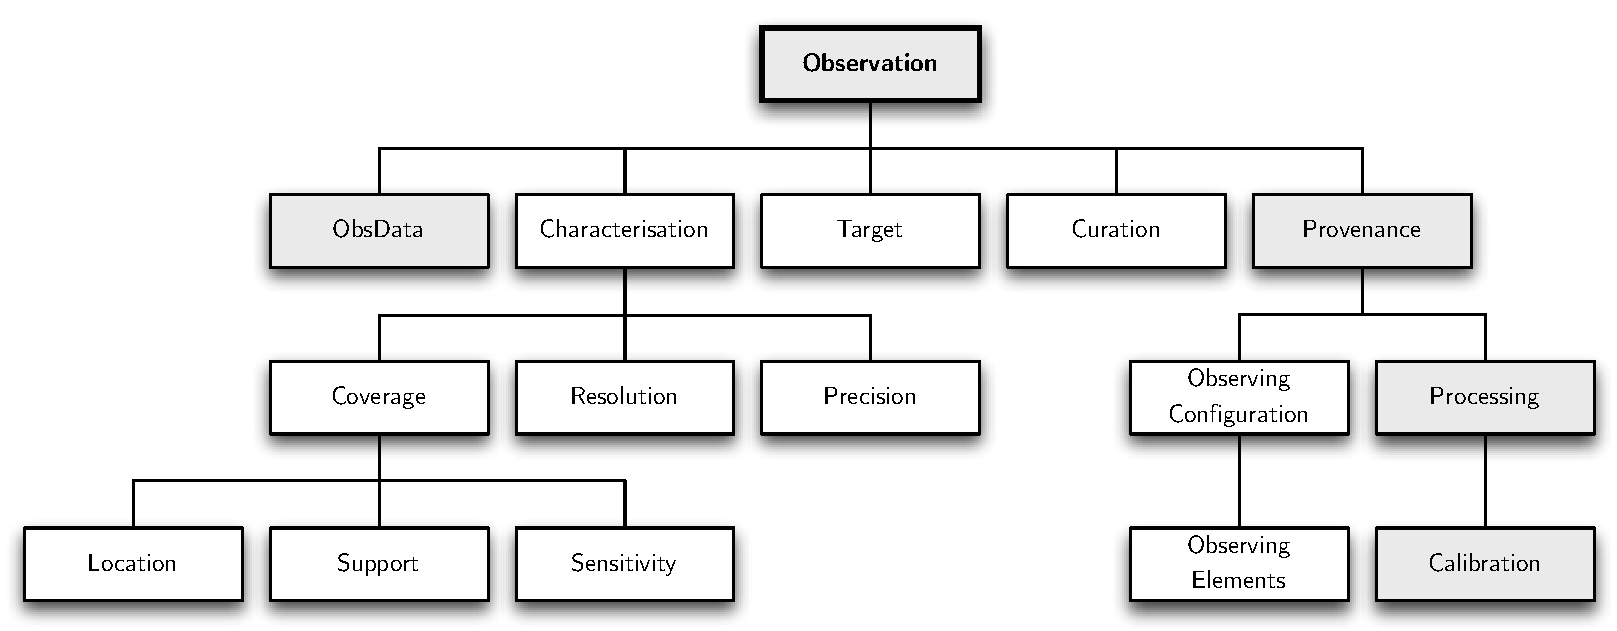
\includegraphics[width=\columnwidth]
					{fig/ObservationDM.pdf}
				\caption[The Observation Data Model]
				{
					 The Observation Data Model. Diagram recreated
					from the \emph{General Model for Observation}
					figure in the Data Model for Observation
					working draft~\cite{2005dmo..rept.....M} from
					2005. The shadowed rectangles show data and
					metadata items which can change in case of a
					reanalysis of the observational data,
					highlighting the essential difference between
					Provenance due to observing configuration setup
					and data processing. The hierarchical
					association does not show object
					cardinality, i.e., the number of times instances
					of an object can be related to its father
					object.
				}
				\label{fig:fig_ObservationDM}
			\end{figure}
			
			First, that figure shows that the main constituents
			of the ObsDM are the dataset Characterisation (where
			in parameter space can the observation be found),
			Target (what is known about the
			target of our observation), Curation (who is reponsible
			for getting this observation into the archive, or
			publishing it into the VO), and Provenance (what has
			been done to the set of photons which correspond to this
			observation).
			
			 The figure also illustrates the main difference between
			two different classes of Provenance: the metadata and
			data that would change in case of a reprocessing of 
			observed data are shadowed in grey. Neither the raw data
			themselves nor their characterisation would change,
			while the data provenance not having to do with the
			observational setup would have to reflect those changes.
			
			Another issue that can be derived from that figure is
			that the Characterisation is one of the most observation
			technique independent sub-data models of the
			Observation, and as such the work on the Observation
			data model was delayed until the Characterisation data
			model was finished.
			
			 We must note that even when the
			STC~\cite{2007stc..ivoa.....R}, and
			CharDM~\cite{2008dmadcrept.....L}, have reached the
			status of Recommendation, the
			ObsDM~\cite{2005dmo..rept.....M} is still an early
			working draft whose main role has been providing
			momentum to the STC and Characterisation efforts.
			\suppress[Enrique]{Once
			the CharDM reaches Recommendation status, the next
			efforts in order to complete the ObsDM are the
			Photometric data model (complementary to spectra), the
			Image data model, and the Provenance data model.}
		
		% subsection the_ivoa_observation_model (end)

		\subsection{Characterisation} % (fold)
		\label{sec:the_ivoa_characterisation_data_model}
			
			\begin{figure}[tbp]
				\centering
					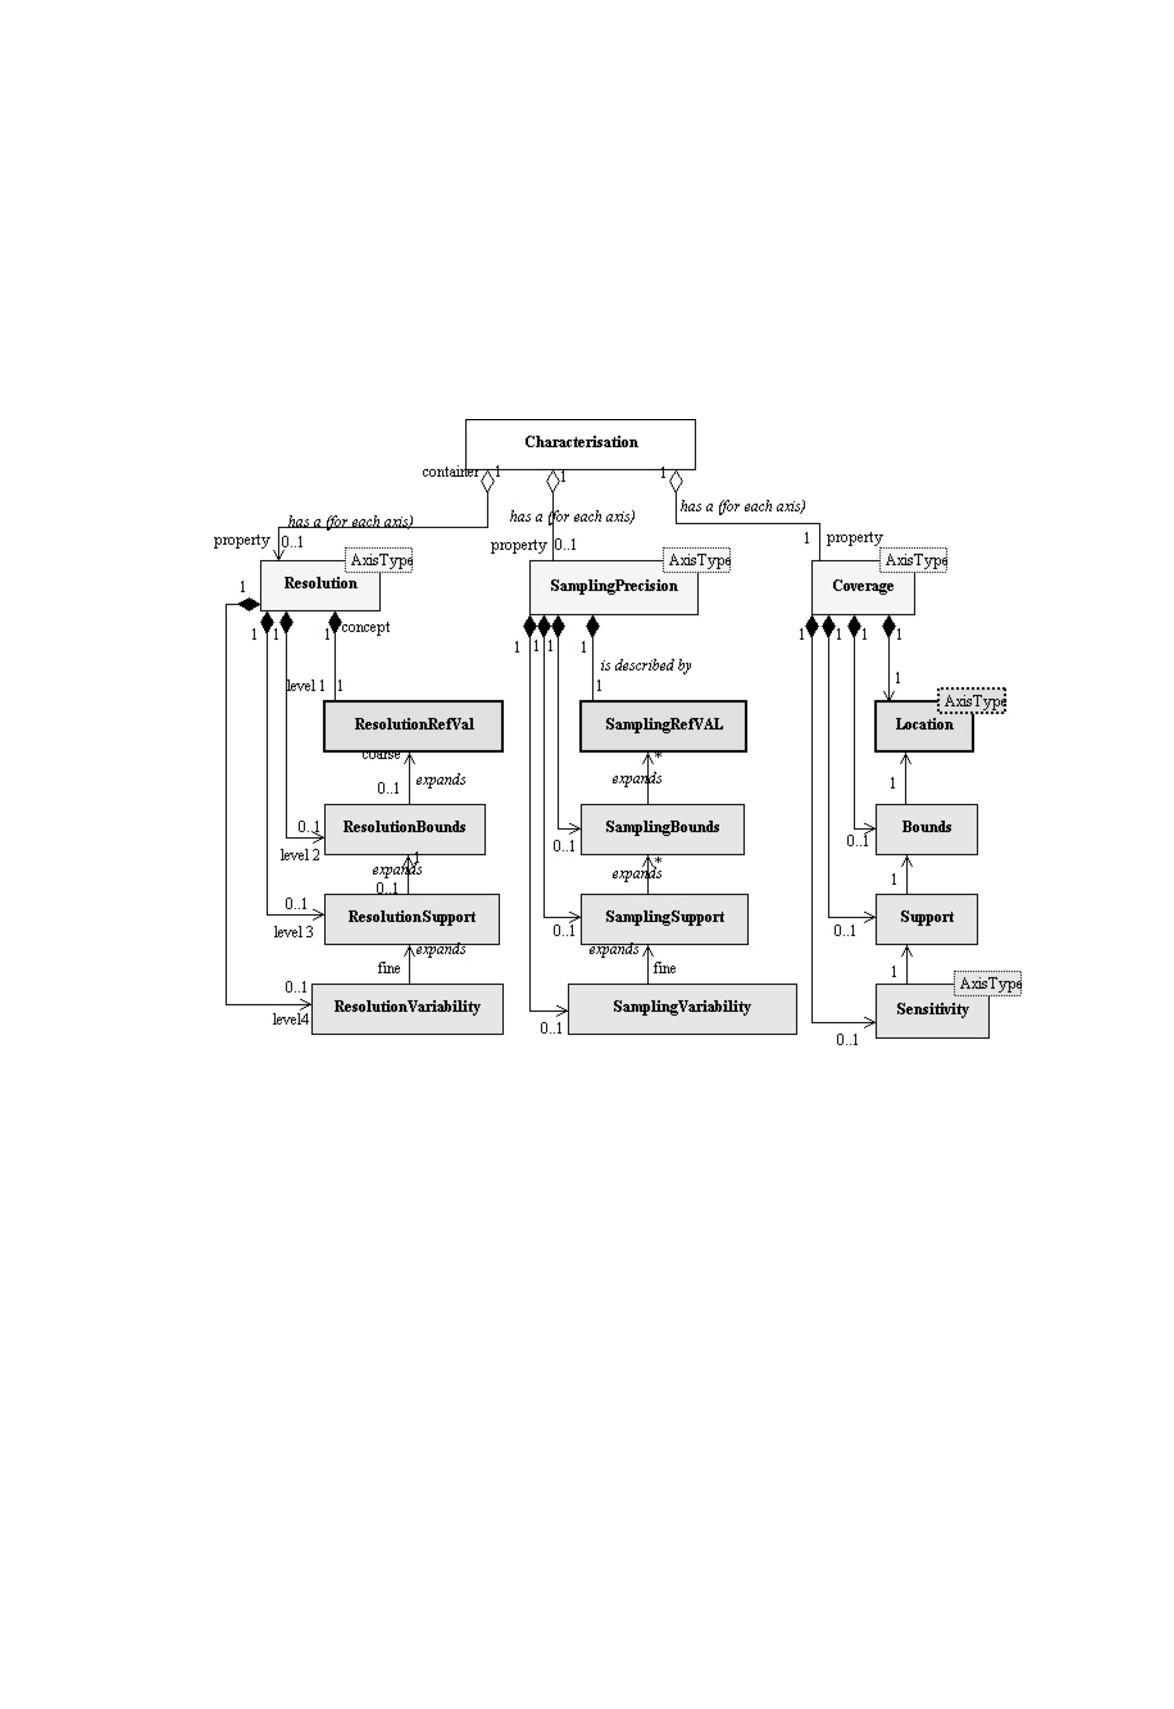
\includegraphics[width=\columnwidth]
					{fig/CharDMPerAxisProperties.pdf}
				\caption[Characterisation Data Model per axis]
				{
					Characterisation Data Model, described per axis,
					as a UML class diagram.
					Reproduced from the CharDM
					recommendation~\cite{2008dmadcrept.....L}.
				}
				\label{fig:fig_CharDMPerAxisProperties}
			\end{figure}
		
			\begin{figure}[tbp]
				\centering
					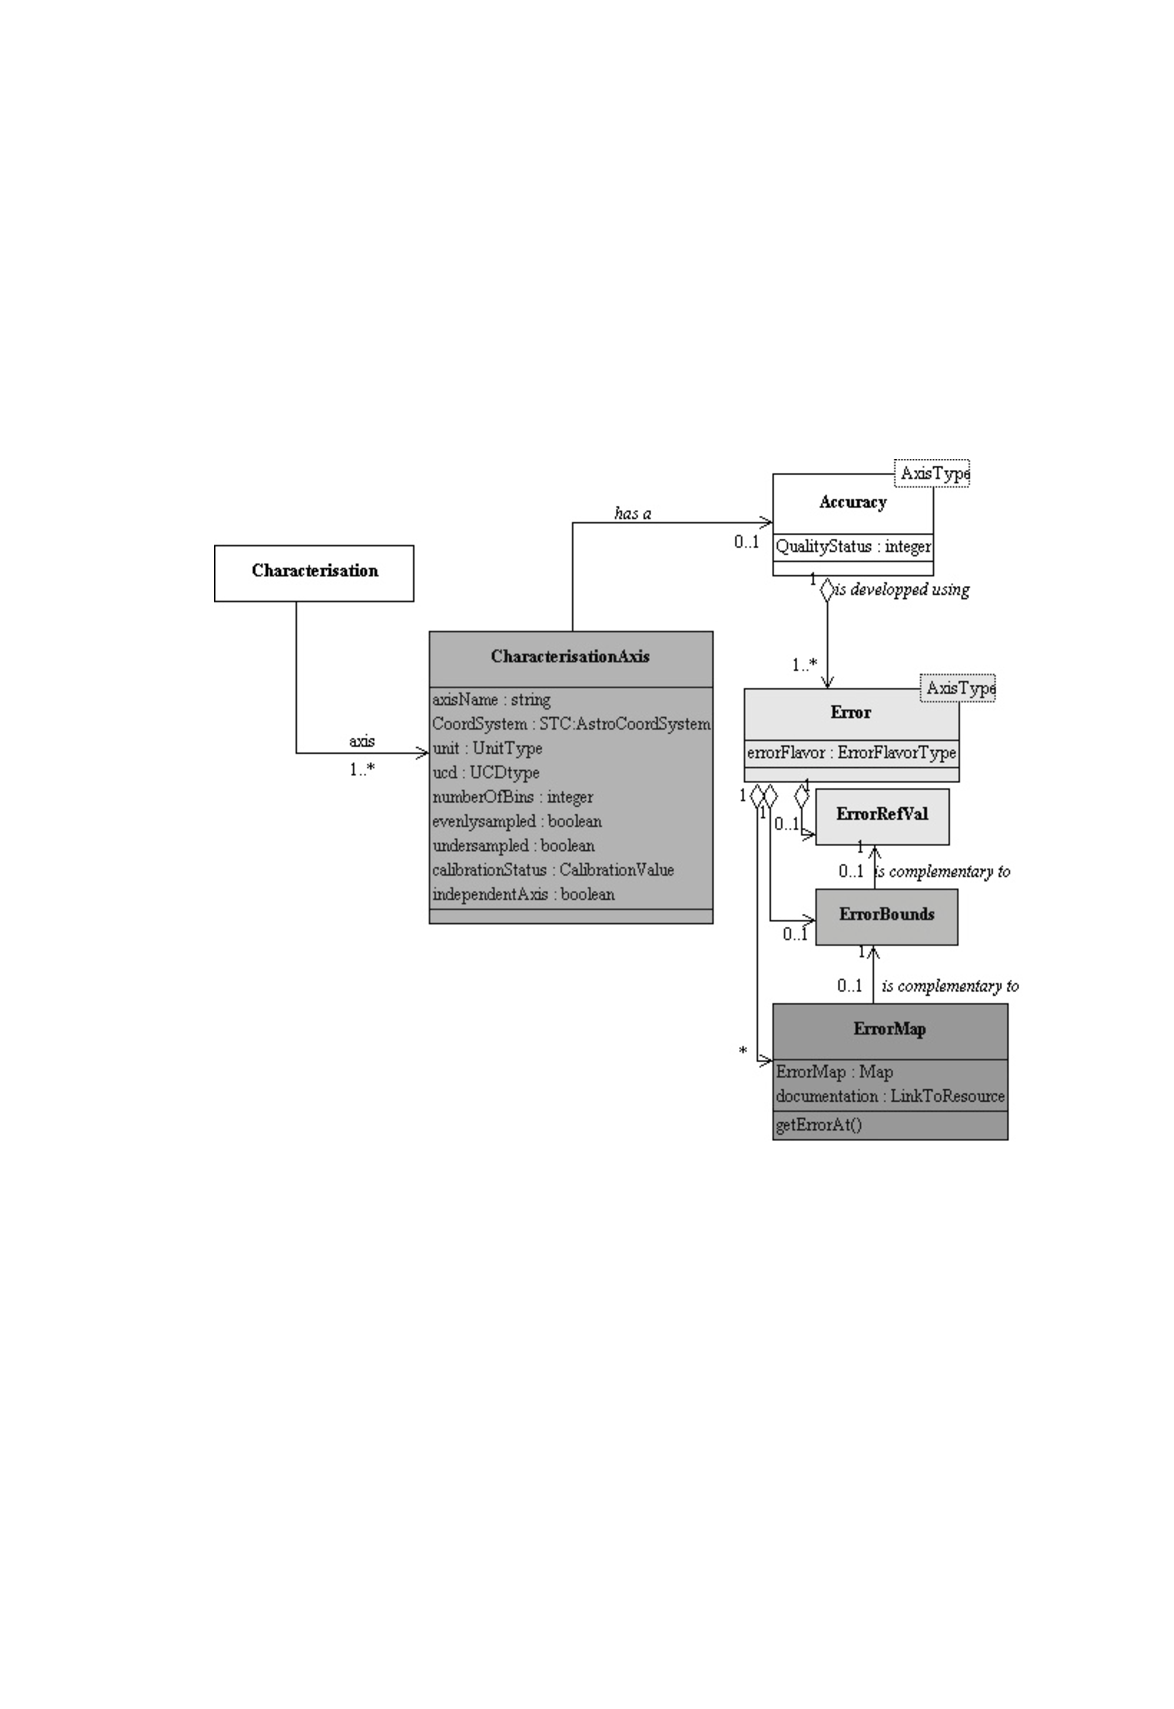
\includegraphics[width=\columnwidth]
					{fig/CharDMAccuracy.pdf}
				\caption[Accuracy class and CharacterisationAxis]
				{
					Each Characterisation instance must contain one
					or more CharacterisationAxis instances, to
					which an optional Accuracy instance can be
					attached.
					Reproduced from the CharDM
					recommendation~\cite{2008dmadcrept.....L}.
				}
				\label{fig:fig_CharDMAccuracy}
			\end{figure}
			
			 As previously said, the Characterisation data model
			(CharDM) deals with the question \emph{Where in
			parameter space is this observation?}, where the
			parameter space is comprised of the observation world
			coordinates (WCS) axis, the time axis, the spectral
			axis (and its complementary velocity axis), and the
			observable axis. Additional axes could be taken into
			account, as the structure for each axis is practically
			identical.
			
			 The CharDM (\emph{Data Model for Astronomical DataSet 
			Characterisation}~\cite{2008dmadcrept.....L}) is
			currently an IVOA Recommendation (since March 2008),
			and it covers all the sub-classes established for the
			CharDM in the ObsDM, but a few more.
			Figure~\ref{fig:fig_CharDMPerAxisProperties} shows the
			current structure of the CharDM per specified axis.
			
			 We can see that a Characterisation instance, composed
			of several CharacterisationAxis instances, each of them
			with a Coverage class, and optional SamplingPrecision
			and Resolution classes. The Coverage class must include
			a Location specification, and if they exist, both the
			SamplingPrecision and Resolution classes must provide
			reference values (RefVal). Both Location and Reference
			values can be optionally further specified by Bounds
			and Support, and a final specification in the form of
			Sensitivity for Coverage, and of Variability for
			SamplingPrecision and Resolution.
			
			 It can also be noticed that the current CharDM
			has evolved with respect to the CharDM outlined with
			the ObsDM draft: there is an additional Bounds class
			related to Coverage in each of the axes to be
			characterised.
			
			 In addition, and not shown in 
			figure~\ref{fig:fig_CharDMPerAxisProperties}, an
			Accuracy class has been added which specifies both data
			quality and errors. Figure~\ref{fig:fig_CharDMAccuracy}
			shows the Accuracy class. Each CharacterisationAxis
			instance can optionally contain an Accuracy instance,
			which is further defined by an Error class which, in
			the same spirit of the remaining Characterisation
			classes, has a RefVal, Bounds, and instead of
			Variability an ErrorMap.
			
			 We can see that the CharDM is an integral
			part of any dataset description to be made, and is as
			observation independent as possible. Indeed, the
			CharDM is also used within the VODataResource service
			description in order to characterise whole archives, or
			particular subsets of interest in the Registry.
			
		% subsection the_ivoa_characterisation_data_model (end)
		
		\subsection{Space and Time Coordinates} % (fold)
		\label{sub:space_and_time_coordinates}
			
			 The Space and Time Coordinates data
			model~\cite{2007stc..ivoa.....R} (STC) was created in
			order to have a systematic way of specifying different
			coordinate systems within the VO.
			
			 While initially the supported coordinate systems for
			VOTables and data access protocols have been Equatorial,
			with the possibility to further specify an epoch, 
			and the IAU has gone a step further with the approval
			of the International Coordinate Reference System (ICRS),
			equatorial coordinates are not
			the natural system for several astronomical disciplines,
			such as Solar System science, or Galactic studies.
			
			 The STC is both a data model (it specifies quantities
			and relationships), but also incorporates two ways of
			expressing serialisations of data model instances:
			STC-X, an XML-based STC serialisation,
			and STC-S, which is string-based and more compact
			and human readable, for use in data models
			where an XML payload cannot be delivered, or ease of
			writing is desirable.
			
			 Within the VO there are three places where the STC can
			be used: data access queries, Characterisation of
			observation Coverage in both the Spatial and Temporal
			axes, and the Object to Position resolution. However,
			for most of the existing VO services, either J2000 or
			ICRS equatorial coordinates are assumed.
			
			 The complexity of the STC stems from the very different
			coordinate systems used in astronomy, and the aim to be
			an all-encompassing effort. A glimpse of its complexity
			can be seen in figure~\ref{fig:fig_STCDM}, which shows
			the most basic STC entities\footnote{And on the STC 
			Recommendation length, which runs at 109 pages.}.
			
			Even when the STC is an IVOA Recommendation, is subject
			to analysis for better embedding in other data models
			(see the Spectrum case in the following section), and
			tools for creating/analysing STC entities are still to
			be developed.
			
			\begin{figure}[tbp]
				\centering
					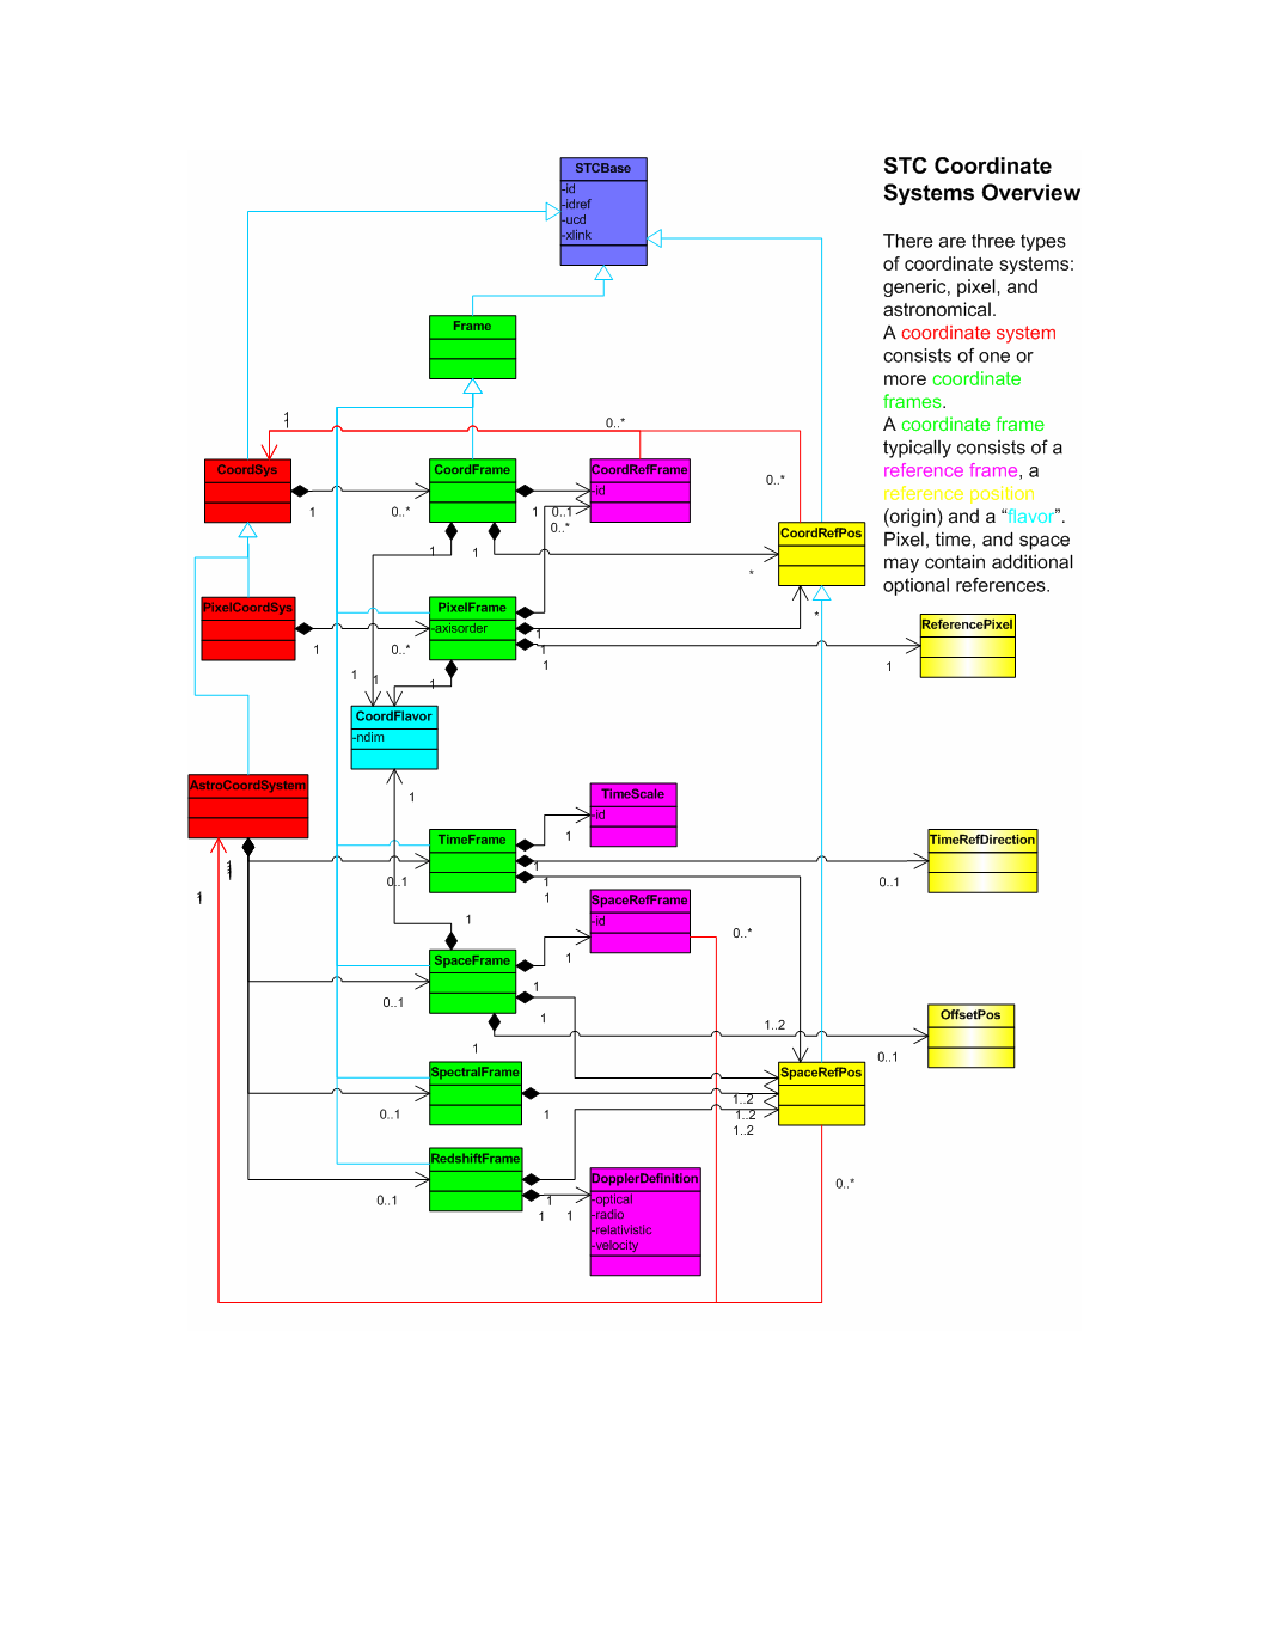
\includegraphics[width=\columnwidth]
					{fig/STCDM.pdf}
				\caption[Space and Time Coordinates data model
				overview]
				{
					An overview of the Space and Time Coordinates
					data model. Reproduced 
					from~\cite{2007stc..ivoa.....R}.
				}
				\label{fig:fig_STCDM}
			\end{figure}
			
			
		% subsection space_and_time_coordinates (end)
		
		\subsection{Spectrum} % (fold)
		\label{sub:spectrum}
			
			\begin{figure}[tbp]
				\centering
					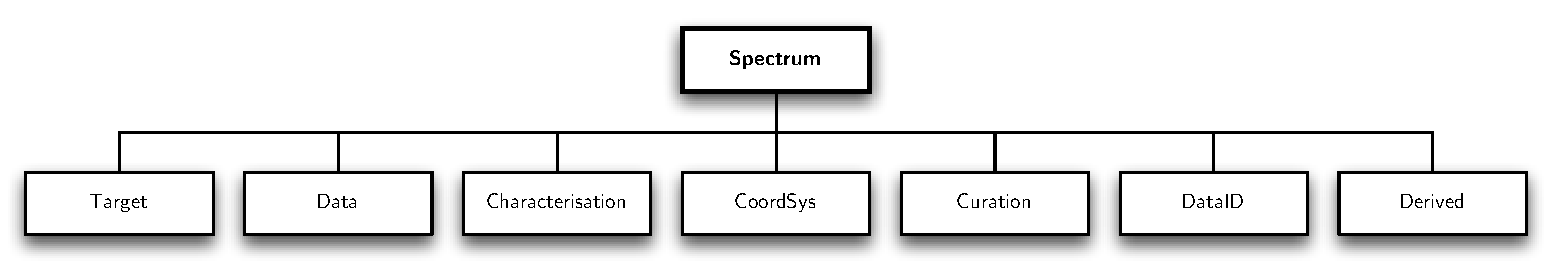
\includegraphics[width=\columnwidth]
					{fig/SpectrumDM.pdf}
				\caption[High-level overview of the Spectral DM]
				{
					High-level overview of the Spectral data model.
					The root class is the Spectrum class, which can
					compared to the Observation class in the ObsDM.
				}
				\label{fig:fig_SpectrumDM}
			\end{figure}
			
			The Spectrum data model (SpecDM) is different from the
			data models above in that it describes a particular
			data product, and not just a generic observation or an
			observation set.
			
			 Figure~\ref{fig:fig_SpectrumDM} shows the high-level
			overview of the Spectrum data model. Compared with the
			ObsDM, ---see fig\-ure~\ref{fig:fig_ObservationDM}--- and
			the CharDM
			---fig\-ure~\ref{fig:fig_CharDMPerAxisProperties}---,
			it can be
			seen that the Spectral data model is based on the
			ObsDM, without specifying a Provenance class; it
			specifies a CoordSys class separate from Target, and
			also a DataID (a simplified data curation for a
			particular entity); and a Derived class for holding
			information which does not belong to the Spectrum, but
			can be derived from it under several assumptions, such
			as the Signal-to-Noise Ration (SNR), Redshift and
			Amplitude variability.
			
			 Due to the already mentioned complexity of the STC,
			the SpecDM uses a simplified version of STC-S entities
			to describe spatial regions (circles and poligons for
			the SpecDM) and temporal coordinates.
			
			 There are many different techniques to obtain spectra,
			and each of them produces a different data product.
			The most important difference concerns on whether the
			spectrum is obtained by a diffraction or refraction
			method, which provides a sampling on wavelength; or if
			the spectrum is obtained via a Fourier transform
			method (from the Fourier transform of an autocorrelation
			signal, for instance), which provides a sampling on
			frequency. As frequency and wavelength for
			electromagnetic radiation are linked by a non-lineal 
			equation ($\lambda = c\nu^{-1}$), it is very important
			for astronomical data processing applications to
			treat each case differently\footnote{To the point that
			the SpecDM recommends using different Spectrum entities
			for spectra which are available both with a frequency
			and a wavelength scale.}.
			
			 The SpecDM has reached IVOA Recommendation status, but
			its Characterisation class is still not fully
			compatible with the last version of the CharDM, as
			sanctioned as IVOA Recommendation. Debate is still
			open on how to use it for time series, instead of the
			time series provisions included in the STC data model.
			Finally, the Spectrum class can only identify one
			single spectrum. Work has yet to start on the
			Spectral Associations data model, in order to describe,
			for instance, On-The-Fly spectra, 3D IFU spectra, or
			any other multidimensional datasets where one of the
			dimensions is frequency, wavelength or velocity.
			
		% subsection spectrum (end)
		
		%\subsection{The DAL model} % (fold)
		%\label{sub:the_dal_model}
		%	
		%	We have mentioned
		%	---section~\ref{sec:role_of_data_models_in_the_vo}---
		%	the DAL data model.
		%	
		%	This simplified model, which 
		%	
		%% subsection the_dal_model (end)
		
	% section existing_ivoa_data_models (end)
	
	\section{Other astronomical data modelling efforts} % (fold)
	\label{sec:other_astronomical_data_modelling_efforts}
		
		Apart from the IVOA data models mentioned above, we have
		reviewed some other data models relevant to astronomical
		observations' data modelling, or data modelling for
		radio astronomical archives.
		
		The only IVOA Note on radio astronomy data prior to the
		publication of the RADAMS was the \emph{Data model for
		Raw Radio Telescope} by Lamb and
		Power~\cite{LamPow0310IVOA}.
		
		Many aspects of our work ---specially controlled
		vocabularies, and the extensibility to interferometry---
		were initially based upon this model.
		
		\newcommand{\asdmurl}[0]
		{http://aramis.obspm.fr/~alma/ASDM/ASDMEntities/}
		Other models reviewed include the data model used for
		publication of the Australian Telescope Compact Array
		(ATCA)~\cite{2006astro.ph..1354}
		archive\urlnote{http://atoa.atnf.csiro.au/}, the scientific
		archive domain model of the National Optical Astronomy
		Observatory (NOAO)~\cite{War04NOAO}
		archives\urlnote{http://archive.noao.edu/nsa/}, and the
		ALMA Science Data
		Model\urlnote{\asdmurl}~\cite{2006ASPC..351..627V}.
		
		A special mention is made of the MPEG-7 and MPEG-21
		overview documents~\cite{Bormans:fk, Martinez:uq},
		available in web-page form at
		\url{http://www.chiariglione.org/}, used as the basis for
		our Policy and Curation sub-models.
		
		
	% section other_astronomical_data_modelling_efforts (end)
	
	\section{Conclusions} % (fold)
	\label{sec:dm_conclusions}
		
		Within the VO, data to be delivered must be described in
		the most complete possible way so that automated selection
		and manipulation tools can rely on that description in
		order to manipulate, select, and ultimately provide
		\emph{understanding} of the described data.
		
		 Both the data themselves and the metadata need to conform
		to a common data model, in order to make interoperability
		between different systems possible. Those data models are
		governed by the IVOA DM WG.
		
		 The only observation-related data model already in
		Recommendation stage is the SpecDM. The other data models
		having reached Recommendation status are the STC data model,
		and the CharDM.
		
		 The SpecDM shows that it is possible to use the ObsDM as
		a template to create an observation-specific data model,
		and both the CharDM and the STC have shown their modularity
		in order to be embedded in other data models. However, 
		STC entities are usually simplified before being properly
		used.
		
		 In order to create a complete VO-compliant data model
		which can hold all kinds of radio observations from
		different single-dish observatories we will provide, then:
		
		\begin{description}
			\item[Compatibility with existing and/or proposed data
			models] Any VO-com\-pli\-ant da\-ta mo\-del should make
			use of existing and recommended IVOA data models, and
			should try to fit themselves within the data model most
			related to the kind of data to be described.
			
			\item[Use of existing data models in similar
			e-Science disciplines] The Vir\-tual Observatory is
			one example of an e-Science based discipline: the
			main success of the VO comes from the federation of
			disperse datasets, and their aggregation through
			network access protocols. As such,
			it would be wise to make use of the existing e-Science
			middleware and conventions for non astronomy-specific
			parts of the system.
			
			\item[Support for spectral associations] 
			The SpecDM provides support for spectral measurements,
			but there is no way to relate spectra taken from
			On-The-Fly observations, or spectra extracted from a
			radio data cube, or maps of continuum measurements.
			This support is added to the RADAMS by combining
			the CharDM and Packaging.
			
			\item[Specification of missing classes] 
			The ObsDM proposed classes for dealing with data
			access Policies, data Provenance, and data Packaging, 
			while the CharDM proposed a Sensitivity class. A
			data model for radio astronomical observations would
			need to provide definitions for such classes.
			
			\item[Support for radio astronomical observing modes]
			There are widely different observing modes in radio
			astronomical, single dish, observatories. A VO data
			model for them would have to support them.
			
			\item[Extensibility for radio interferometric
			observations] Most of the data model details can be
			generalised for radio interferometric observations,
			and where possible the way to extend the data model
			in order to support interferometric observations is
			made explicit.
		\end{description}
		
		We will address these requirements in the following chapters.
		
	% section dm_conclusions (end)
	
	%% section radio_dm_needs (fold)
	%\section{Needs for a radio astronomical observation data model} 
	%\label{sec:radio_dm_needs}
	%
	%	Radio astronomical observations can be defined as those
	%	performed in the radio band,
	%	%(from 13~MHz to the 1~THz range),
	%	and for single dish radio telescopes can be classified as:
    %
	%	\begin{description}
	%		\item[Total flux] measures all the incoming energy in
	%		the receiver's bandwidth, typically measured by
	%		non-coherent receivers, or derived by integration of
	%		the signal received by coherent receivers. This kind of
	%		measurement is also called continuum measurement.
	%		
	%		\item[Spectrum] a frequency-dependent energy
	%		distribution across a given bandwidth, and with a given
	%		resolution.
	%	\end{description}
	%	
	%	As there are emission sources other than the astronomical
	%	source being studied, a reference signal must be obtained
	%	and subtracted form the total signal coming from the source
	%	of interest. The reference signal can be obtained:
	%	
	%	\begin{description}
	%		\item[By switching positions] The radio sky is
	%		typically obscure. By moving away from a radio source,
	%		we are effectively measuring the sky contribution.
	%		There are several ways of switching positions: changing
	%		to an absolute, fixed sky position, or switching to a
	%		position which is at a certain angular distance from
	%		the observed position, and keeps the distance while
	%		mapping across a source. Further divisions can be made
	%		on how is the switching performed: by moving the
	%		antenna, by moving the secondary mirror (always a
	%		relative position switching), or by using a chopper
	%		wheel, for instance.
	%		
	%		\item[By switching frequency] Radio sources typically
	%		follow a power law in their intensity, while sky noise
	%		follows a flat distribution. By switching to lower
	%		frequencies, we can sample the amount of sky noise,
	%		which can then be subtracted of our intended signal.
	%		
	%	\end{description}
	%	
	%	Another difference is on antenna tracking:
	%	
	%	\begin{description}
	%		\item[Fixed tracking] with fixed tracking, the antenna
	%		movement is just enough to track a single position
	%		in celestial coordinates; only data from a single
	%		coordinate (other than reference
	%		measurements) are obtained.
	%		
	%		\item[Point to point tracking] the antenna can be pointed
	%		to different coordinates, and obtain data from each of
	%		them.
	%		
	%		\item[On-the-fly tracking] in this case, the antenna
	%		follows a pattern across the sky, and measurements are
	%		continually recorded, so that there is not a single
	%		position which can be attributed to each measurement,
	%		but instead the measurement is assigned to a segment
	%		of the sky. However, the advantage of this kind of
	%		tracking is the faster mapping of the sky with a
	%		similar signal to noise ration. In any case, the
	%		paths described across the sky need to be specified.
	%		
	%		\item[Solar system tracking] the tracking methods
	%		imply positions are fixed in the celestial sphere, but
	%		for solar system objects the object orbit has to be
	%		computed, and the tracking system made to follow that
	%		orbit, instead of just tracking the movement of the sky.
	%		
	%	\end{description}
	%	
	%	In brief, a data model for radio astronomical observations
	%	needs to provide metadata for:
	%	
	%	\begin{itemize}
	%		\item Project related information, in order to be able
	%		to query on PI, or a whole observation project.
	%		
	%		\item Observation characterisation information: where
	%		in the celestial sphere, time, bandwidth and observed
	%		flux axes is comprised an observation.
	%		
	%		\item Telescope and instrument setup information.
	%		
	%		\item Ambient conditions information.
	%		
	%		\item Processing steps performed on the selected data.
	%		This includes identifying the final data product
	%		being delivered, and the way the reference signal is
	%		obtained.
	%	\end{itemize}
	%	
	%	But, in addition, the following needs have also to be
	%	fulfilled:
	%	
	%	\begin{itemize}
	%		\item Provide data access policy information. We will
	%		include it in a Policy class, and we will take
	%		inspiration from the Policy classes available for
	%		accessing restricted media, such as those proposed by
	%		the MPEG-7 and MPEG-21 standards.
	%		
	%		\item 
	%	\end{itemize}
	%
	%% section radio_dm_needs (end)


% chapter data_modelling_in_the_vo (end)


	%2345678901234567890123456789012345678901234567890123456789012345678901
%\newcommand{\classname}[1]{\textsc{#1}}

% chapter radams (fold)
\chapter[Radio Astronomical DAta Model for Single-dish radio
telescopes]
{RADAMS: a Radio Astronomical DAta Model for Single-dish radio
telescopes}
\label{cha:radams}
	
	In the past chapters we have been making emphasis on how the VO
	works by providing common data access protocols, common data
	formats for information interchange, and a common data model
	for expressing, within the constraints of the data model and
	data access protocols of the VO, the description of
	observational data.
	
	In particular, in the previous chapter we have shown the
	general framework proposed by the IVOA for describing whole
	observations, characterising the parameter space occupied by
	them, and using a specific format/data model for indicating
	space and time restrictions. We have also seen that the
	Observation data model is not complete, while the CharDM and
	STC are mature enough to have been granted the IVOA
	Recommendation status. However, they have never been applied to
	radio astronomical archives, and have never been used as the
	basis for a radio astronomical archive.
	
	In this chapter we will try to answer the question: \emph{How
	to architecture a VO-compatible radio astronomical archive?},
	and for that we will use the outlined ObsDM as a foundation in
	order to create a complete data model for radio astronomical
	observations which can be used both for the development of
	single-dish radio astronomical archives, enhancing the existing
	IVOA Observation data model at the same time.
	
	\section{Basic requirements of astronomical archives} % (fold)
	\label{sec:radams_archive_basics}
		
		We will start stating the obvious: a radio astronomical
		online archive has to provide a way for astronomers to find
		and retrieve radio astronomical observations. The most
		simple incarnation of such an archive would include a
		complete list of all observation files, together with a
		system for retrieving the actual file containing the
		observational data set.
		
		With such a simple archive system only people aware of what
		was observed and contained in each file would be able to use
		it. Thus, the most basic additional requirement all
		astronomers would need is coordinate searching, or the
		ability to identify files with positions in the celestial
		sphere.
		
		The next requirement in order of importance is the
		identification of the band of the electromagnetic spectrum
		being scanned by the instrument, \invisiblenote{when
		different bands are observable.} as different bands provide
		diverse information on the physical processes taking place
		in the observed region. This is the first place where the
		specifics of radio astronomy begin to emerge.
		
		These pieces of information  do not actually belong
		to the science data themselves, and are metadata for the
		observation. In particular, the two examples above can be
		identified to the lowest levels of detail in the CharDM
		for the spatial and spectral axes (Location and Bounds in
		both axes).
		
		This small example tells us two things: first, it shows
		that the most important metadata needed for information
		filtering are already part of the proposed IVOA data models;
		and second, that such data models can be used as a
		blueprint for astronomical archives
		
		\begin{figure}[tbp]
			\centering
			
			\subfloat[][]
			{
				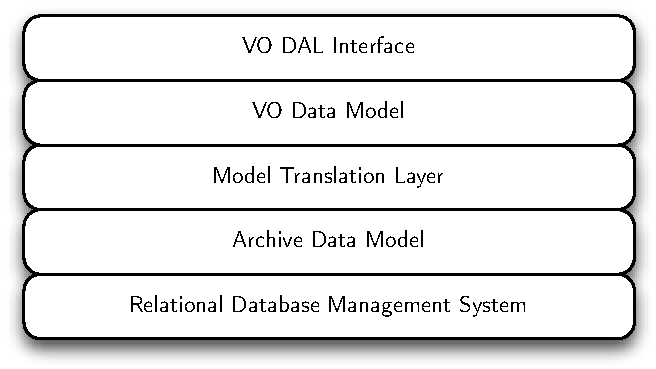
\includegraphics[width=0.47\columnwidth]
				{fig/VODalArchiveLayers.pdf}
				\label{subfig:fig_VODalArchiveLayers}
			} 
			\hfill 
			\subfloat[][]
			{
				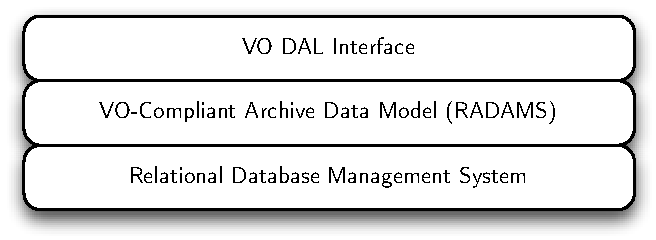
\includegraphics[width=0.47\columnwidth]
				{fig/VORadamsLayers.pdf}
				\label{subfig:fig_VORadamsLayers}
			} 
			\caption[Data modelling layers for different kinds of VO
			archives]
			{
				Data modelling layers for different kinds of VO
				archives. Subfigure
				\subref{subfig:fig_VODalArchiveLayers} shows the
				layered structure of a VO archive built on an
				existing, while~\subref{subfig:fig_VORadamsLayers}
				shows the simplicity of an archive built from
				scratch for VO compatibility.
			}
			\label{fig:VODalRadamsArchiveLayers}
		\end{figure}
		
		A welcome side-effect of directly using VO data 
		models as the basis for astronomical archives is that
		their use simplifies the archival development, and the
		integration of fully described archives in the VO.
		
		To illustrate this,  we will compare the
		development layers and complexity needed to build VO
		compatibility both on existing archival systems, and 
		by building an archive from scratch.
		Figure~\ref{fig:VODalRadamsArchiveLayers} shows both
		kinds of archives side by side.
		
		In the case of an archive with an already existing
		infrastructure
		---sub\-fi\-gu\-re~\ref{subfig:fig_VODalArchiveLayers}---,
		VO data models have to be mapped on top of a translation
		layer in charge of creating VO entities from the existing
		archive data model. But if the archive is going to be built
		from scratch, the Data Access Layer (DAL)
		interfaces\footnote{The DAL data model and interface will
		be briefly described in relation with the different data
		products to be delivered.} can be built on top of the VO
		entities directly provided by the archive infrastructure
		---in the case of
		sub\-fi\-gu\-re~\ref{subfig:fig_VORadamsLayers}, the
		RADAMS---.
		
		It should be noticed that for building VO archives on top
		of an existing, non-VO archive, the translation layer has
		to provide some metadata which do not only need
		translation, but in many cases those metadata have to be
		extracted or even calculated from either the FITS headers,
		the actual FITS data tables/images, or even the observation
		logs\footnote{Possibly, even a combination of all of
		them. Actual examples will be shown in the chapter devoted
		to radio astronomical characterisation with the RADAMS.}.
		
		\suppress[Enrique]{
		Not all the pieces of information needed to build the whole
		RADAMS metadata come directly from the FITS data, but
		instead come from observing logs, or as mentioned before,
		from the actual data, and might be lost if they are not
		explicitly stated. Creating a new archive conforming to
		IVOA data models ensures the availability of the data
		sources for the VO metadata, and allows for an ideally
		direct translation between the archive and DAL layers.}
		
	% section radams_archive_basics (end)
	
	\section{RADAMS requirements and overview} % (fold)
	\label{sec:radams_requirements_overview}
		Once established that a VO-based data model can indeed be
		used as the basic architecture for an astronomical
		archive, we can define which will be the requirements of
		such a data model for radio astronomical observations,
		our RADAMS.
		
		\begin{description}
			\item[Based on the Observation and Characterisation DMs]
			The RADAMS is a da\-ta model for the metadata regarding a
			radio astronomical single-dish observation, and as such
			is based on the Observation data model. In order to
			complete the RADAMS, extensions are provided within the
			framework of the ObsDM and the CharDM.
			
			\item[Separation of data and metadata] In a RADAMS
			based archive, data will be stored in the form of FITS
			files or VOTables, whereas all metadata will be stored
			in database form complying with the RADAMS. For already
			existing archives, this condition is relaxed, but a
			query mechanism for all RADAMS metadata should be
			available.
			
			\item[Single-feed observations] Metadata and
			observations are considered always to be referring a
			single feed. If a telescope or instrument is able to
			provide several feeds simultaneously, each one will be
			stored separately, and will refer to the same observing
			proposal, but will have a separate existence.
			
 			\item[Radio astronomical data products] The RADAMS will
 			be able to support data of the following kinds:
			
			\begin{itemize}
				\item Single-pointing flux measurements;
				
				\item Single-pointing radio astronomical spectra,
				or spectra associations;
				
				\item On-the-fly on-off, spectra data, or 
				continuum flux observations, in the form of images
				and data cubes;
			\end{itemize}
			
			The data product definition must be made compatible
			with existing IVOA DAL protocols: images (SIA protocol),
			sets of
			spectra (SSA protocol), and coordinates-based data tables.
			
		\end{description}
		
		From those requirements, we have built the RADAMS data
		model, whose high-level structure is shown in
		figure~\ref{RADAMSHLoverview}. We can see that we have
		closely followed the ObsDM, and the CharDM, and that in
		order to use 
		the whole ObsDM we will need to provide definitions for
		some of the classes.
		
		\begin{figure}[tbp]
			\begin{center}
			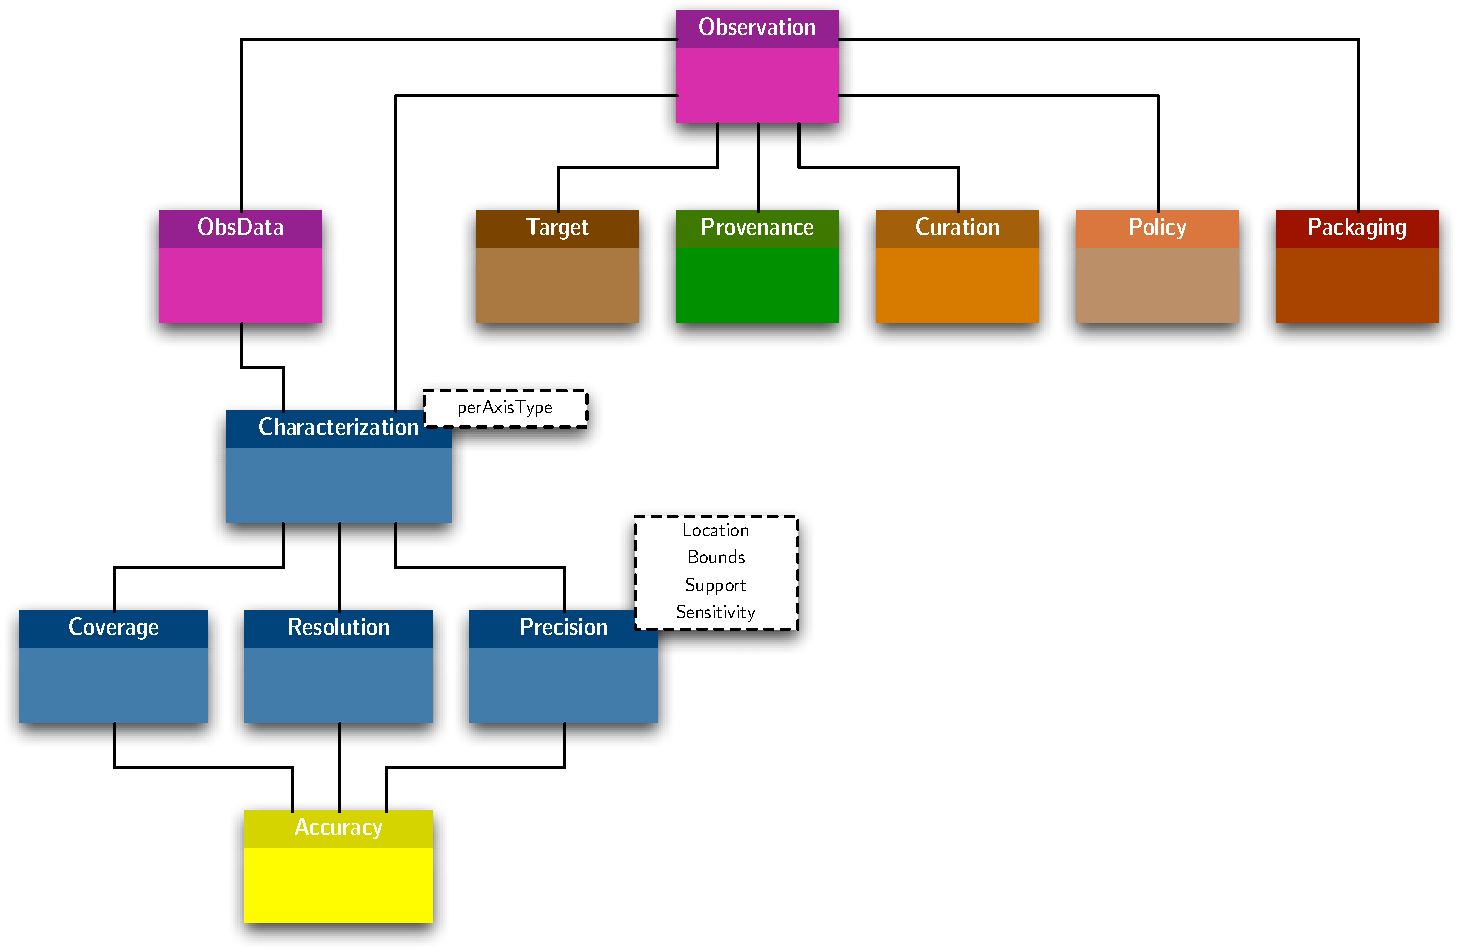
\includegraphics[width=\columnwidth]
				{fig/RADAMS_Complete}
			\caption[RADAMS general class organisation]{
				RADAMS general class organisation. Different colours
				correspond to different sub-models, and will be
				kept in the next chapters.
			}
			\label{RADAMSHLoverview}
			\end{center}
		\end{figure}
		
		Those classes and sub-models defining the RADAMS will be,
		then:
		
		\begin{description}
			\item[Observation] Root class for the data model. It
			works as a hub to which both actual observational data
			(ObsData) and the remaining metadata are linked
			together.
			
			\item[ObsData] Describes how to access the actual
			data being described by all the RADAMS' classes.
			
			\item[Target] Describes the target of the observation,
			providing as much information as available for
			already known targets.
			
			\item[Characterisation] Corresponds to the CharDM
			classes.
			
			\item[Provenance] Links all the information regarding
			the origin of the observation, both from an
			administrative, technical and scientific point of
			view.
			
			\item[Curation] Describes who is responsible for
			maintaining a particular observation, a set of
			observations, or all of the archive.
			
			\item[Policy] Is used to specify the access rights
			for different systems and persons accessing the
			archive.
			
			\item[Packaging] Describes the way an observation,
			or a set of observations, are actually delivered
			when the archive is queried.
		\end{description}
		
		We will describe these classes in the following sections,
		and we will leave their exact implementation details to
		specific chapters.
	% section radams_requirements_overview (end)

	\section{Observation and ObsData} %(fold)
	\label{sec:observation_obsdata}

		The Observation class is the root class of the data model.
		It describes an arbitrarily large dataset that can be
		derived directly from an observation, or from several
		observations. Generally, we will consider an Observation as
		the set of data recorded with the same instrumental
		setting, and with the same associated target during a
		continued period of time.

		% In the particular case of the DSS-63, an Observation would
		% be made of the set of on/off observations associated with
		% the same target, or the final, flux calibrated spectra. As
		% we will see later, the Packaging class will allow us to
		% have different degrees of granularity for data access.
		
		On the other hand, the ObsData class is a proxy class
		representing the actual data, and holding a reference that
		the archive interface can use to retrieve or provide
		science-ready data files.
		
		The Observation class, then, is used to link together
		the different aspects of the observation, from the
		originating proposal (Curation) to the reduced data
		(ObsData), and taking into account also the data
		Characterisation, the data access Policy, etc.
		
		However, a direct link is also preserved between the
		ObsData and the Characterisation, so that if data is
		repackaged the mapping to the Characterisation metadata can
		be preserved.
		
		The Observation class, then, only needs a unique identifier
		for each unique observation, what brings to the table what
		is the minimum observation (in practice, ObsData) to be
		collected by the RADAMS. We will answer that in the next
		chapter.
		
		% For sets which can be provided either as individual
		% datasets, or as joined 
		% The RADAMS makes use of the Packaging class ---which we
		% will define below--- in order to specify what particular
		% pieces of data are being retrieved. Besides, the archival
		% of continuum information cannot be discarded, as most radio
		% telescopes are capable of performing continuum scans.
				
	% section observation_obsdata (end)
	
	
	\section{Characterisation} %(fold)
		
		The Characterisation class
		provides
		the quantitative and qualitative description of the
		observational data in multiple axes. This information is
		stored conforming to the most current CharDM IVOA
		Recommendation~\cite{2008dmadcrept.....L}.
		
		As seen in the previous chapter, we can consider that any
		astronomical measurement occupies a position in a
		multi-di\-men\-sion\-al space, defined by several axes.
		Initially, this axes are just four (but more can be added):
		spatial (coordinates), temporal, spectral, and a fourth
		axis corresponding to the observed physical quantity (e.g.,
		measured flux, or polarisation, in the case of radio
		observations). Characterisation gives us a description of
		the data in different attributes and levels of detail
		inside this multi-di\-men\-sion\-al space, including
		physical units and scales.
		
		The Characterisation class for each individual axis
		can be divided in the following
		subclasses:
		
		\begin{description}
			\item[Coverage] Specifies which part of the
			multi-di\-men\-sion\-al space has been encompassed by
			the measurement. That is, when was the observation made
			and for how long, which field was covered, which bands
			were studied, what was the range of observed flux, and
			so on. Each of those questions belongs to a different
			axis.
			
			 \item[Resolution] Specifies data resolution in each of
			the axes. Resolution is independent of the sampling, as
			it is a property of the instrument/observing process.
			
			 \item[Precision] When data are sampled in any
			of the axes
			(e.g., for spectral data in the frequency domain, data
			are sampled by means of filter banks, or by FFT from 
			an autocorrelation signal),
			this class will include information on
			the sampling precision\footnote{This is different from
			resolution: resolution is a property of the instrument,
			due to uncertainties on the energy distribution of the
			source, because of convolution of the source’s and the
			instrument’s profiles.}.
			
			\item[Accuracy] Specifies the minimum error rate
			achievable for each axis, both from systematic and
			random errors.
		\end{description}
		
		From this group we can see that for Coverage, Resolution and
		Precision information can be defined
		\emph{a priori} for a whole observing program (in the
		Characterisation of a Registry entry, for instance), but they
		can be different for each actual observation dataset, and
		those will be the ones stored by the RADAMS.
		
		In contrast, Accuracy information needs to
		be evaluated \emph{a posteriori}: the lower bounds of 
		accuracy can be known from instrument calibration and
		knowledge of the observation process, but for some axes
		assessing the accuracy actually achieved needs access to
		historical information.
		
		
		
			
		%	 \item[Sensitivity] This class quantifies the
		%	sensitivity of the instrument in the given axis, by
		%	means of a sensitivity function that is defined for the
		%	whole coverage of the observation in the given axis.
		%	This class has not been fully defined yet by the IVOA
		%	Working Group, hence we are providing a tentative
		%	description of this class, in order to help the the
		%	efforts of the Characterisation Working Group.
			
		
	% section Characterisation (end)
	
	\section{Target/Field} %(fold)
	\label{sec:radams_target}
		
		As we have mentioned several times, astronomers study most
		of the time objects they already know, while other times
		they probe a certain part of the sky to see if there is
		something new, or even survey a whole region in order to 
		later exhaustively study that region and all objects they
		can find in it.
		
		This class allows the RADAMS to include information 
		about observed targets. Such target can be mapped to
		known astronomical objects, to detected sources, to a given
		field, et cetera. Having this entity in a separate class from
		the Observation one allows to perform queries by Target, and
		the ability to link external target information using VO
		services (such as Sesame, Aladin, the SkyNode interface,
		et cetera).
		
		In order to be linked with ObsData and Observation
		classes, the unique identifier for the observation is
		stored, which allows for queries on given targets to
		return observations, but also for observation sets to
		retrieve Target information.
		
	% section Target (end)
	
	\section{Provenance} %(fold)
		
		This class groups all the information describing the way
		an astronomical dataset was originated.
		It has to include the instrumental
		setting for that particular observation, coordinates for
		the telescope, weather and atmospheric conditions, and all
		the information about data pre- and post-processing,
		when such data were created by processing already existing
		datasets\footnote{This is already the case for reduced data,
		which makes extensive use of calibration information,
		background models and measurements, et cetera.}.
		
		Again, the link with ObsData is the unique observation
		identifier, but for some of the information, which are
		recorded automatically by the engineering data collection
		systems, time-stamps will need to be used to bound the
		relevant information (for instance, focus and pointing
		calibration observations).
		
	 % section Provenance (end)
	
	\section{Policy} % (fold)
		
		In astronomy, observation data are the property of the
		investigator having suggested and planned the observation,
		for a period which in some cases depends completely on the
		observer, which might decide never to release to the public
		the observations he made, and in other cases depend on
		policies implemented by the organisation providing the
		observing facility. Typical cases are 12 to 24 months of
		proprietary data from the moment the observation was
		performed to the moment the observation is made available
		to the general community.
		
		Some observatories have policies where different access
		rights are available depending on the country or the
		organisation a particular investigator belongs to, due
		to different agreements between the hosting organisation
		and data requesting parties.
		
		This class allows both for the tagging of the observation
		data, and for establishing the data access rights for 
		datasets depending on the Policy information for the 
		dataset itself, and for the user.
		
		Examples of widely different data access policies can be
		found in archives such as the European Southern Observatory
		Archive\footnote{The archive of the ESO, for instance, makes
		header information (including pointing) available
		immediately after observation, together with calibration
		data. Actual science data are only released after a
		proprietary period (which can be extended under demand),
		together with observation proposal abstracts. Their policy
		can be found at
		\url{http://archive.eso.org/cms/eso-data-access-policy}}
		(ESO). A more general view on scientific data access
		policies can be found on the Committee on Data for Science
		and Technology (CODATA) of the International Council for
		Science (ICSU) on their Scientific Data Policy Statements
	website\urlnote{http://www.codata.org/data_access/policies.html}.
		
		In order to accommodate all these different kinds of data
		access policies, we have chosen a role-based approach,
		where different permissions are allowed not to each
		different user, but regarding the role that user has
		against a particular piece of information. This mechanism
		will be discussed in detail in chapter~\ref{sec:policy}.
		
	% section Policy (end)
	
	\section{Curation} %(fold)
		
		To be considered part of the VO community, all VO resources
		have to be included in a Registry. The Curation class
		encompasses all the metadata needed for well-formed archive
		and data VO registry. In addition, we also integrate an
		ObservingProgram subclass, proposed by Anita Richards in
		the ObsDM document~\cite{2005dmo..rept.....M}, which acts
		as an intermediate class that allows grouping together
		different observations with a common goal, such as a any
		kind of survey, or follow-up observing program, for
		instance.
		
		Curation information is generated first for the whole
		archive, and later on different observations can be
		associated (via a Packaging different from the default
		for the archive) with a different curator, so that they
		can either be properly registered as a different resource,
		or at least downloaded, packaged data, can refer to the
		curator for that particular collection.
		
	% section curation %(end)
	
	\section{Packaging} %(fold)
		
		Archive queries result in different datasets, and a
		particular dataset for a given Observation can contain
		several measurements. The Packaging class specifies what is
		being delivered by the archive as a result for a given
		query, and the organisation of data packages different
		VOTables link to. We will provide an initial development of
		this class, suitable for the needs of the RADAMS. We will
		also propose a VO general packaging system, the VOPack.
		
		The principles for the VOPack are providing an off-line
		mechanism for assessing the main properties applicable to
		the whole package of datasets: complete Characterisation of
		Coverage, Resolution, and Precision in all relevant axes,
		together with common Curation, Policy, Targets and
		Data Provenance.
		
	% section Packaging (end)
	
	\section{Conclusions} % (fold)
	\label{sub:radams_conclusions}
		
		In this chapter we have shown that a complete version of
		the ObsDM can be used as a blueprint for building
		astronomical archives, making easier the task of building
		VO services publishing the archive assets.
		
		In a high-level overview, the needs for radio astronomy
		are quite similar to the needs of astronomy in general:
		data need to be accessed by coordinates, targets and
		then spectral and temporal filters applied. We have also
		shown that the differences for radio astronomical
		observations lie in the Characterisation part, specially
		in Spectral coverage, and also in spatial resolution; and
		in the Provenance class, which deals with the details on
		how was the observation observed.
		
		With those specifics in mind, we have built the RADAMS, a
		Radio Astronomical DAta Model for Single-dish observations,
		which will be used both as a valid blueprint for building a
		radio astronomical archive from scratch, by virtue of its
		implementation of the ObsDM and the CharDM, and the
		specification of yet to be defined by the IVOA data models
		within the ObsDM.
		
		In particular, the data models receiving the most attention
		from the RADAMS are:
		
		\begin{description}
			\item[Characterisation] Need to characterise 
			radio astronomical observations from their particular
			properties.
			
			\item[Provenance] The origin of the observation in
			radio astronomy is fundamentally different from that
			of optical observations, as the optical
			path\footnote{Even for non-optical (or non-visible)
			electromagnetic radiation the path followed by photons
			inside a photon collection instrument is called the
			optical path. The means for making photons of different
			wavelengths follow a particular optical path is, as it
			can be imagined, dependent of the wavelength range.}
			and detectors are completely different in nature.
			
			\item[Packaging] This model, in principle, has no radio
			astronomical specifics, but it has been developed as a
			way to provide different kinds of associated
			observations together. In a sense, is a complement to
			the SpecDM (and the ObsDM) lack of a way to declare
			that several observations are not to be independently
			considered, but that instead form a coherent unit for
			scientific analysis.
			
			\item[Target] Again, this model should not be,
			in principle, specific to radio astronomy. It has
			been defined in a way as general as possible as to
			be used for the SpecDM, the ObsDM, and also be able
			to host information from services such as Simbad,
			VizieR, and NED, dealing with compilations of
			information for named/catalogued sources.
		\end{description}
		
		As a result, we will provide specific guidance for the
		serialisation of radio astronomical observations in the
		next chapter, while we will provide additional details on
		the Curation, Packaging and Policy data models on
		chapter~\ref{cha:radams_curation_packaging_and_policy},
		leaving the subject of data provenance to
		chapters~\ref{cha:data_provenance_in_the_vo} and
		\ref{cha:radams_data_provenance}.
	
	% section radams_conclusions (end)	
	
% chapter radams (end)
	%2345678901234567890123456789012345678901234567890123456789012345678901
% chapter radamscharobs (fold)
\chapter[RADAMS: Characterising radio astronomical observations]
[RADAMS: Characterising radio observations]
{RADAMS: Characterising radio astronomical observations} 
\label{cha:radamscharobs}
	
	\invisiblenote{
		The most important data model to implement is the CharDM.
		Characterisation allows systems querying a VO registry to
		find which datasets contain some data of interest (because
		of the region of the sky, the spectral band, sensibility,
		et cetera), and later on evaluate if the query results are
		indeed of interest.
		
		 In this chapter we will develop the Characterisation data
		model for radio astronomical observations,
		
		 After this initial overview of the classes that conform
		the RADAMS, we will detail the attributes corresponding to
		each of the classes of the model.
	}
	
	In the previous chapter we analysed how an astronomical archive
	could be built using the basis of the ObsDM, if the missing
	data models suggested by the ObsDM document were to be
	implemented. We also illustrated how VO compatibility could be
	added to archives built on such a basis much more easily.
	
	After that, we showed the high level overview of the RADAMS,
	which was at first glance almost indistinguishable from the
	ObsDM, something which is indeed a feature of the RADAMS.
	Finally, we provided a first overview of the definition of
	each particular class and sub-models, and the way they mesh
	together.
	
	Once we have introduced the RADAMS,  we will start studying it
	in detail in this and the following chapters.  In particular,
	this chapter will be devoted to how the RADAMS stores the
	Observation and ObsData information, and how the 
	CharDM data model is filled for the different observation
	modes in radio telescopes.
	
	In addition, in those chapters devoted to the
	detailed exploration of the RADAMS, we will select appropriate
	FITS Keywords  and UCDs for FITS and VOTable serialisations of
	observational data.  FITS Keywords will be selected first from
	the official FITS mandatory headers~\cite{Hanisch:1999fk}.  If
	no mandatory   keyword exists,   they will be chosen  from the
	Multi-Beam FITS Raw Data Format~\cite{MudPolHat0512Multi-Beam},
	and lastly from the NRAO GBT FITS data
	format~\cite{PreCla0412Device}\footnote{Sometimes those
	keywords cannot appear in the main header of a FITS file, but
	instead in a FITS extension table, but that will not be
	specified.}. Where \texttt{assign} appears, it means
	that a suitable FITS keyword has yet to be
	selected for that particular database attribute.
	
	UCDs will be selected from the UCD1+
	vocabulary~\cite{2005ucv..rept.....P}, using the recommended
	juxtaposition technique in order to clarify the meaning of any
	given term. In some cases, there are no existing UCD atoms, and
	no UCD atom combination, properly describing the attribute. In
	those cases, we will propose corresponding UCD unique atoms,
	for stand-alone or combined use.
	
	We also want to acknowledge the initial effort by Lamb
	and Power in creating a draft for an IVOA
	Note~\cite{LamPow0310IVOA} in which radio astronomical data were
	initially modelled. Many of the controlled vocabularies
	proposed in this and the following chapters have used that
	document as a source.
	
	\invisiblenote{
		char•ac•ter•ize |ˈkariktəˌrīz| 
		verb [ trans. ] 
		1 describe the distinctive nature or features of : the historian characterized the period as the 
		decade of revolution. 
		2 (often be characterized) (of a feature or quality) be typical or characteristic of : 
		the disease is characterized by weakening of the immune system. 

		ob•serve |əbˈzərv| 
		verb [ trans. ] 
		1 notice or perceive (something) and register it as being significant : [with clause ] 
		young people observe that decisions are made by others. 
		• watch (someone or something) carefully and attentively : Rob stood in the hallway, 
		where he could observe the happenings on the street. 
		• take note of or detect (something) in the course of a scientific study : the behavior 
		observed in groups of chimpanzees. 

		ob•ser•va•tion |ˌäbzərˈvā SH ən| 
		noun 
		1 the action or process of observing something or someone carefully or in order to 
		gain information : she was brought into the hospital for observation | detailed observations 
		were carried out on the students' behavior. 
		• the ability to notice things, especially significant details : his powers of observation. 
		• the taking of the altitude of the sun or another celestial body for navigational 
		purposes. 
	}
	
	\section{ObsData and Characterisation} %(fold)
	\label{subObsDataCharacterisation}
		
		Following the IRAM MultiBeam FITS definition
		document~\cite{MudPolHat0512Multi-Beam}, based on the ALMA
		Software Glossary~\cite{Schwarz:2003zr}, we can define
		several degrees of observational data in radio astronomy:
		
		\begin{description}
			\item[Dump] This is the smallest interval of time for
			which a set of correlated data can be accumulated and
			output from the backend stage.
			
			 \item[Integration] Set of dumps, all identical in
			configuration, which are accumulated and form the basic
			recorded unit.
			
			 \item[Sub-scan] Set of integrations performed while
			the antennas complete an elemental pattern across the
			source: e.g., an azimuth displacement on a pointing 
			source, a focus displacement within a focus calibration,
			et cetera.
			
			 \item[Scan] Set of sub-scans with a common goal, such
			as a pointing scan, a focus scan or an atmospheric
			amplitude calibration scan, among others.
		\end{description}
			
		Hence, the minimum useful unit to be recorded in the
		archive is the sub-scan, which can be appropriately
		described, but the minimum scientifically significant unit
		is the scan, so depending on the kind of granularity
		desired one could base the archive upon one or the other.
		Higher order units ---such as multiple scans on the same
		source, for enhancing the signal-to-noise ration, or
		scans to different sources belonging to the same observing 
		program--- should be derived from Project metadata.
		
		 To link together these scans with the rest of the data model
		we will use the ObsData class
		(which could also be referred to as \classname{RawData}) as the root
		class for the RADAMS. From ObsData instances, we will form
		a tree of data that will describe a particular scan, both
		by its properties in the Spatial, Temporal, Spectral, and
		Observable axes, and its respective Accuracy.
		
		 We show a high level overview of the ObsData class and its
		relationships with AxisFrame, Coverage, Resolution, and
		Accuracy classes in figure~\ref{figObsData}. Compare it 
		with figures~\ref{fig:fig_CharDMPerAxisProperties} and
		\ref{fig:fig_CharDMAccuracy}.
		
		
		\begin{figure}[tbp]
		\begin{center}
		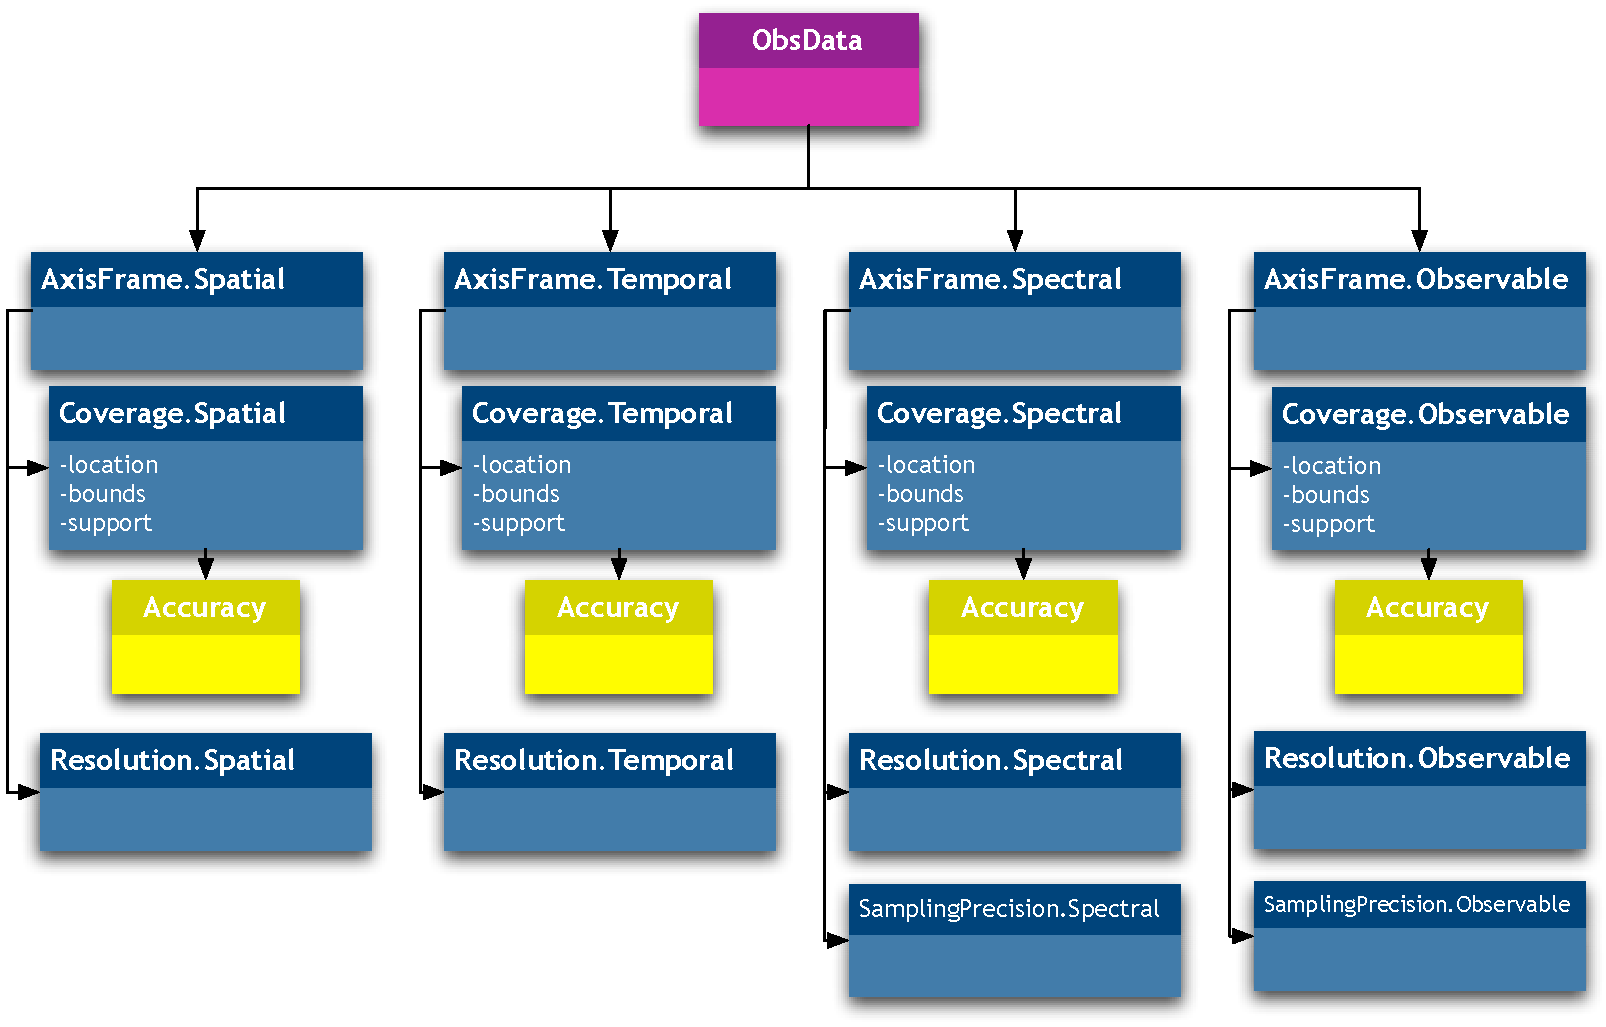
\includegraphics[width=\columnwidth]{fig/ObsData-DM}
		\end{center}
		\caption[ObsData class data model]{
			ObsData class data model; the different axes for the
			Characterisation part of the data model are shown.
		}
		\label{figObsData}
		\end{figure}
		
		\begin{description}
			\item[ObsData] Instances of this class (also to be
			referred as RawData) will contain the final data. As
			discussed previously, we will keep either whole scans
			to determine the scientific data, or processed data
			(such as spectra).
		
			 \item[AxisFrame] Instances of this class will contain
			metadata that describe properties of the axis,
			such as units, calibration state, et cetera.
		
			 \item[Coverage] We will describe the position of the
			archived data in the parameter space: where and when was
			the telescope pointed, and what wavelength range was
			observed. Several subclasses exist:
		
			\begin{description}
				\item[Location] This subclass of each Coverage
				axis
				describes the characteristic value for each of
				them.
				For instance, in the spatial axis
				Coverage.Spatial.Location would be set to
				the central point of the observed field, and for
				the temporal axis
				Coverage.Temporal.Location would hold 
				either the middle or the start
				time of the scan.
				
				\item[Bounds] Maximum and minimum values
				of the axis; for instance, Coverage.Spectral.Bounds
				would give us the maximum and minimum frequencies
				of the spectrum, and Coverage.Tem\-po\-ral.Bounds
				would give us the starting and ending time of the
				observation.
				
				\item[Support] Set of parameters in that
				axis where we have valid observational data. For
				instance, in the temporal axis
				Coverage.Tem\-po\-ral.Sup\-port could be
				a set of intervals when data were gathered,
				excluding the pauses for reissuing scans.
				
				\item[Sensitivity] Sensitivity is an
				additional refinement to Support, where for the
				sections of the axis with Support for the observation
				a response function of the instrument in
				the given axis is provided.
				This is especially useful for cases with a large
				number of small interruptions in the data, there is
				need for data resampling, filter
				profiles have to be accounted for, and so on.
			\end{description}
			
			We have to remember that these subclasses form a
			hierarchy by which Location is mandatory, and all
			further refinements optional, but for a refinement
			to appear all levels above it must appear to: for
			instance, we can provide just Location, but if Support
			appears, Bounds needs to appear as well.
		
			\item[Resolution] Instances of this class are used to
			describe resolution in each axis. For instance,
			Coverage.Spatial.Resolution would be defined in 
			single-dish observations by the Half-Power Beam
			Width (HPBW).
			
			 \item[SamplingPrecision] For a sampled axis ---such as
			the Spectral axis, in the case of spectroscopic
			data---, an instance of this class will hold sampling
			precision, described as a pixel scale.
			
			 \item[Accuracy] All of the aforementioned classes
			should have an accompanying class in order to describe
			errors and data quality for each axis. In the case of
			archives without data mining capabilities, we only have
			to provide Accuracy instances related to the Coverage
			classes.
			
		\end{description}
		
		\invisiblenote
		{\textbf{Refine this paragraph with better description of
		errors and their handling.} It has to be noted that, for
		some observational sets, there is no meaningful definition
		of an error. Instead, one can define statistical error
		estimations valid for a certain period, and apply those
		definitions for observations being performed during said
		period. That would be the case, for instance, of errors in
		pointing or focus, where one cannot specify the error for a
		single observation, but pointing or focus error averages.}
		
		\subsection{AxisFrame.Spatial and Coverage.Spatial} % (fold)
		\label{ssubSpatialAxis}
			
			In this subsection, we describe the classes that
			configure the description of the spatial axis
			(AxisFrame.Spatial), and the characterisation of the
			coverage in such axis (Coverage.Spatial).
			Figure~\ref{figAxisFrameSpatial} shows the classes and
			their relationships.
			
			\begin{figure}[tbp]
			\begin{center}
			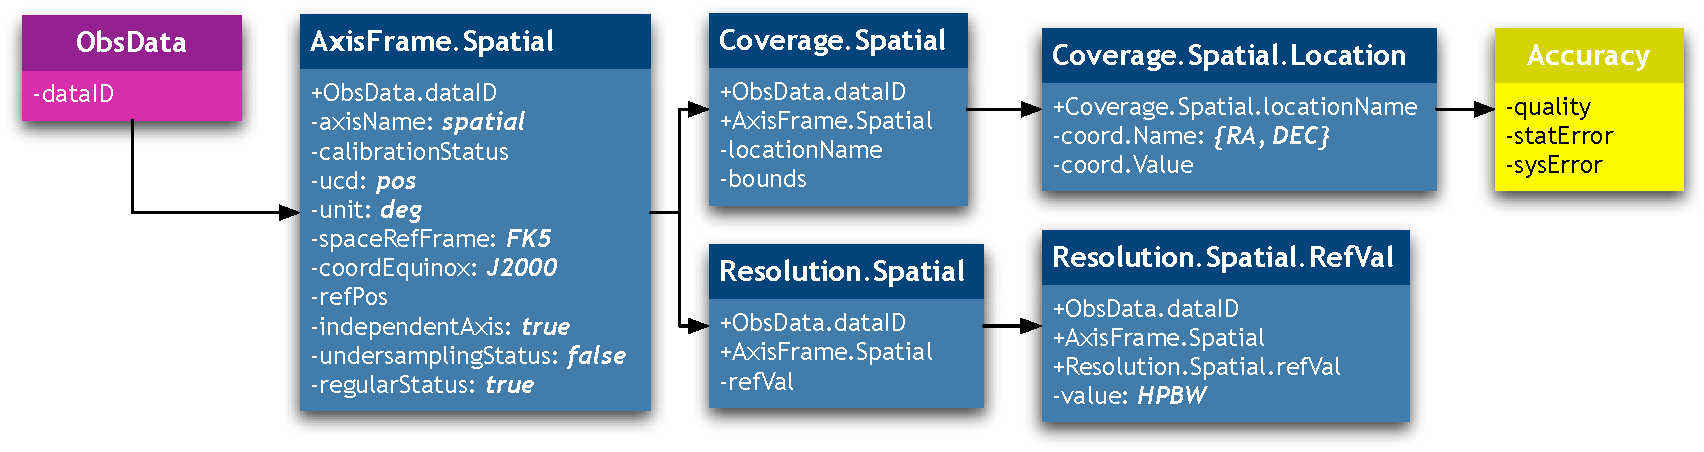
\includegraphics[width=\columnwidth]
			{fig/AxisFrame-Spatial-DM}
			\end{center}
			\caption[Spatial axis frame metadata]
			{
				Spatial axis frame and coverage metadata.
				\todoinlinesuspended{Redo figure with Bounds, Support,
				Sensitivity.}
			}
			\label{figAxisFrameSpatial}
			\end{figure}

			\begin{description}
				\item[AxisFrame.Spatial] This instance describes
				the properties of the Spatial axis, such as
				calibration status, units (normally, degrees),
				reference frame, epoch, spatial sampling type and
				sampling status, et cetera.
				
				 For the DSS-63 antenna, the spatial axis is never
				sampled (because we are not storing maps at this
				stage), and each scan only needs two pairs of
				coordinates (plus pointing accuracy) to describe
				the antenna-pointing pattern.
				
				\invisiblenote{Redo discussion, taking into account
				mappings, and the enhancements for interferometry.}
				
				 As the coordinate space is in this case
				bi-dimensional, and properties for one of the
				coordinates do not have to be equal for the other,
				we should either choose between a vector approach,
				using two dimensional arrays of coordinates, or
				splitting the Spatial classes in different
				subclasses. We choose the first approach, and thus
				all AxisFrame.Spatial attributes will have a
				space-separated array of values (just two values
				separated with an space, for a bi-dimensional
				coordinate space).
				
				 If the archive were to be exploited in the third
				dimension, an additional distance and/or redshift
				coordinate should be entered. As we have seen,
				extension in the spatial axis is straightforward. A
				second option would add an additional axis to the
				Characterisation data model.
				
				 \item[Coverage.Spatial.Location] For the DSS-63
				antenna, the stored values for this class
				correspond to the antenna pointing coordinates.
				If a Target is linked, Spatial.Location information
				sould be the same, unless the target is not directly
				associated, but found by
				cross-correlation with the Targets database.
				
				 \item[Coverage.Spatial.Bounds] Bounds for spatial
				data would be the maximum and minimum for spatial
				coordinates (normally, right ascension and
				declination) when observing the source. For single
				point spectroscopic data, this class is not needed,
				as the antenna does not describe any path across
				the source.
				
				 \item[Coverage.Spatial.Support] Typically, the
				stored values for this class should be equal to
				those of Coverage.Spatial.Bounds, except when
				invalid data within Coverage.Spatial.Bounds might
				exist, or in order to describe an elaborate
				scanning path on the source. This class would
				describe such a path.
				
				 \item[Coverage.Spatial.Sensitivity] In the case of
				the DSS-63 antenna, Spatial.Sen\-si\-tivity would
				be defined as the beam pattern of the antenna,
				in principle in 1D taking symmetries into account,
				but 2D could be considered, as it would be the
				case for a synthesised beam in interferometry.
				Another possibility is the combination of beam
				pattern with receiver efficiency at different
				elevations.
			\end{description}
			
			\invisiblenote
			{\textbf{Rewrite taking into account OTFs, and mappings.
			We already have tables for Spatial.Bounds, .Support
			and even .Sensitivity.}
			Bear in mind that Coverage.Spatial.Support for radio
			astronomical measurements is either a point, for
			spectroscopic calibrations, or a set of line paths for
			bolometric and/or continuum mappings. Spatial support
			will be defined as the set of line paths, and can be
			described by an array of start/end value pairs for 2D sky
			coordinates\footnote{In fact, that is exactly the way 
			paths across the sky for OTF observations are stored
			by the IRAM~30m New Control System.}.
			
			 For spectroscopic data, this class is redundant, as
			mentioned above.}
			
			\begin{table}
			\begin{minipage}{\linewidth}
			\caption[AxisFrame.Spatial metadata]{AxisFrame.Spatial metadata.}
			\begin{smallertabular}{p{3.15 cm}p{1.5cm}p{2.25cm}p{4.35cm}}
				
					& \textbf{FITS} & & \\ \textbf{Attribute} &
			                 \textbf{Keyword} & \textbf{UCD} &
			                 \textbf{Description}\\ \midrule axisName &
			                 \texttt{assign} & \texttt{meta.id; meta.main} &
			                 Axis name.\\ \addlinespace calibrationStatus &
			                 \texttt{assign} & \texttt{obs.calib; meta.code} &
			                 Calibration status from a controlled vocabulary:
			                 \texttt{un\-cal\-i\-brated},
			                 \texttt{cal\-i\-brated},
			                 \texttt{rel\-a\-tive}\footnote{\texttt{rel\-a\-tive}
			                 refers to calibrated data, except for an additive
			                 or multiplicative constant.},
			                 \texttt{normalized}\footnote{\texttt{normalized}
			                 refers to dimensionless quantities, such as those
			                 resulting from the division between two
			                 commensurable datasets.}. \\ \addlinespace ucd &
			                 \texttt{assign} & \texttt{meta.ucd; meta.main} &
			                 Main UCD for the axis.\\ \addlinespace unit &
			                 \texttt{assign} & \texttt{meta.unit; meta.main} &
			                 Main units for the axis.\\ \addlinespace refPos &
			                 \texttt{assign} & \texttt{meta.ref; meta.id} &
			                 Identification of the origin position within the
			                 spaceRefFrame from a controlled vocabulary; See
			                 Space-Time Coordinate Data
							 Model~\cite{Rot0503Space-Time}. \\ \addlinespace
							spaceRefFrame
			                 & \texttt{WCSNAME} or \texttt{RADESYS} &
			                 \texttt{pos.frame; meta.id} & Identification of
			                 the reference system from a controlled
			                 vocabulary; see Space-Time Coordinate Data
							 Model~\cite{Rot0503Space-Time}: \texttt{FK4},
			                 \texttt{FK5}, \texttt{ELLIPTIC},
							 et cetera.\\ \addlinespace
			                 coordEquinox & \texttt{assign} & \texttt{pos;
			                 time.equinox} & Equinox (only if needed).\\
			                 \addlinespace epoch & \texttt{assign} & \texttt{pos;
			                 time.epoch} & Epoch (only if needed).\\ \addlinespace
			                 independentAxis & \texttt{assign} & \texttt{pos;
			                 obs.param; meta.code} & Boolean flag indicating
			                 whether the axis is independent of the rest or
			                 not.\\ \addlinespace undersamplingStatus &
			                 \texttt{assign} & \texttt{pos; obs.param;
			                 meta.code} & Boolean flag indicating whether the
			                 data are sampled in this axis or not.\\ \addlinespace
			                 regularStatus & \texttt{assign} & \texttt{pos;
			                 obs.param; meta.code} & Boolean flag used in case
			                 of sampled data, indicating whether sampling is
			                 regular or not.\\ \addlinespace
			\end{smallertabular}
			\label{tabAxisFrameSpatialMetadata}
			\end{minipage}
			\end{table}

			\begin{table}
			\caption[Coverage.Spatial.Location metadata]
			{Coverage.Spatial.Location metadata.}
			\begin{smallertabular}{p{2.15 cm}p{1.5cm}p{2.25cm}p{5.35cm}}
								& \textbf{FITS} & & \\ \textbf{Attribute} &
			                    \textbf{Keyword} & \textbf{UCD} &
			                    \textbf{Description}\\ \midrule coord.name &
			                    \texttt{assign} & \texttt{pos; meta.name} & Name
			                    of the coordinate whose value goes in
			                    coord.value.\\ \addlinespace coord.value &
			                    \texttt{assign} & \texttt{pos; meta.number} &
			                    Numeric value for the coordinate coord.name.\\
			                    \addlinespace
			\end{smallertabular}
			\label{tabCoverageSpatialLocationMetadata}
			\end{table}

			\begin{table}
			\caption[Coverage.Spatial.Bounds metadata]
			{Coverage.Spatial.Bounds metadata.}
			\begin{smallertabular}{p{2.15 cm}p{1.5cm}p{2.25cm}p{5.35cm}}
								& \textbf{FITS} & & \\ \textbf{Attribute} &
			                    \textbf{Keyword} & \textbf{UCD} &
			                    \textbf{Description}\\ \midrule coord.name &
			                    \texttt{assign} & \texttt{pos; meta.name} & Name
			                    of the coordinate whose value goes in
			                    coord.value.\\ \addlinespace coord.maxValue &
			                    \texttt{assign} & \texttt{pos; meta.number;
			                    stat.max} & Minimum numeric value for the
			                    coordinate coord.name.\\ \addlinespace coord.minValue &
			                    \texttt{assign} & \texttt{pos; meta.number;
			                    stat.min} & Maximum numeric value for the
			                    coordinate coord.name.\\ \addlinespace
			\end{smallertabular}
			\label{tabCoverageSpatialBoundsMetadata}
			\end{table}

			\begin{table}
			\caption[Coverage.Spatial.Support metadata]
			{Coverage.Spatial.Support metadata.}
			\begin{smallertabular}{p{2.15 cm}p{1.5cm}p{2.25cm}p{5.35cm}}
								& \textbf{FITS} & & \\ \textbf{Attribute} &
			                    \textbf{Keyword} & \textbf{UCD} &
			                    \textbf{Description}\\ \midrule code &
			                    \texttt{assign} & \texttt{pos; meta.name} & Code
			                    for the interval where we will be defining
			                    support; an array of [coord.code, startValue,
			                    endValue] tuples can be used to define spatial
			                    support.\\ \addlinespace startValue & \texttt{assign} &
			                    \texttt{pos; meta.number} & 2D start
			                    value.\\ \addlinespace endValue & \texttt{assign} &
			                    \texttt{pos; meta.number} & 2D end
			                    value.\\ \addlinespace
			\end{smallertabular}
			\label{tabCoverageSpatialSupportMetadata}
			\end{table}

			\begin{table}
			\begin{minipage}{\linewidth}
			\caption[Coverage.Spatial.Sensitivity metadata]
			{
					Coverage.Spatial.Sensitivity metadata\footnote{Symmetrical beam
			        patterns could be defined just in one dimension, with pairs of
			        [theta, response] values.}.
			}
			\begin{smallertabular}{p{2.15 cm}p{1.5cm}p{2.25cm}p{5.35cm}}
								& \textbf{FITS} & & \\ \textbf{Attribute} &
			                    \textbf{Keyword} & \textbf{UCD} &
			                    \textbf{Description}\\ \midrule theta[n] &
			                    \texttt{assign} & \texttt{pos.posAng} & Theta
			                    angle for the n\thsup{} beam pattern normalised
			                    response.\\ \addlinespace phi[n] & \texttt{assign} &
			                    \texttt{pos.posAng} & Phi angle for the n\thsup{} beam
			                    pattern normalised response.\\ \addlinespace response[n]
			                    & \texttt{assign} & \texttt{arith.factor} & N\thsup{}
			                    normalised beam pattern response.\\ \addlinespace
			\end{smallertabular}
			\label{tabCoverageSpatialSensitivityMetadata}
			\end{minipage}
			\end{table}

			\begin{table}
			\caption[Coverage.Spatial.Resolution metadata]
			{Coverage.Spatial.Resolution metadata.}
			\begin{smallertabular}{p{2.15 cm}p{1.5cm}p{2.75cm}p{4.85cm}}
								& \textbf{FITS} & & \\ \textbf{Attribute} &
			                    \textbf{Keyword} & \textbf{UCD} &
			                    \textbf{Description}\\ \midrule
			                    referenceValue & \texttt{assign} &
			                    \texttt{pos.angResolution} & Resolution reference
			                    value.\\ \addlinespace
			\end{smallertabular}
			\label{tabCoverageSpatialResolutionMetadata}
			\end{table}

			\begin{table}
			\caption[Accuracy.Spatial metadata]{Accuracy.Spatial metadata.}
			\begin{smallertabular}{p{2.15 cm}p{1.5cm}p{2.25cm}p{5.35cm}}
								& \textbf{FITS} & & \\ \textbf{Attribute} &
			                    \textbf{Keyword} & \textbf{UCD} &
			                    \textbf{Description}\\ \midrule quality &
			                    \texttt{assign} & \texttt{pos; meta.code.qual}
			                    &Quality code for spatial coordinates; invalid
			                    data are flagged with a quality code of 1.\\
			                    \addlinespace sysError & \texttt{assign} & \texttt{pos;
			                    stat.error.sys} &Systematic error for spatial
			                    coordinates.\\ \addlinespace sysErrorHigh &
			                    \texttt{assign} & \texttt{pos; stat.error.sys;
			                    stat.max} & Maximum systematic error for spatial
			                    coordinates.\\ \addlinespace sysErrorLow &
			                    \texttt{assign} & \texttt{pos; stat.error.sys;
			                    stat.min} & Minimum systematic error for spatial
			                    coordinates.\\ \addlinespace statError & \texttt{assign}
			                    & \texttt{pos; stat.error} &Statistical error for
			                    spatial coordinates.\\ \addlinespace statErrorHigh&
			                    \texttt{assign} & \texttt{pos; stat.error;
			                    stat.max} & Maximum statistical error for spatial
			                    coordinates.\\ \addlinespace statErrorLow &
			                    \texttt{assign} & \texttt{pos; stat.error;
			                    stat.min} & Minimum statistical error for spatial
			                    coordinates.\\ \addlinespace
			\end{smallertabular}
			\label{tabAccuracySpatialMetadata}
			\end{table}

		% subsection ssubSpatialAxis (end)

		\subsection{AxisFrame.Temporal and Coverage.Temporal} % (fold)
		\label{ssubTemporalAxis}
			
			In this subsection, we describe the classes that
			configure the description of the temporal axis
			(AxisFrame.Temporal), and the characterisation of the
			coverage in such axis (Coverage.Temporal).
			Figure~\ref{figAxisFrameTemporal} shows the classes and
			their relationships.
			
			\begin{figure}[tbp]
				\begin{center}
				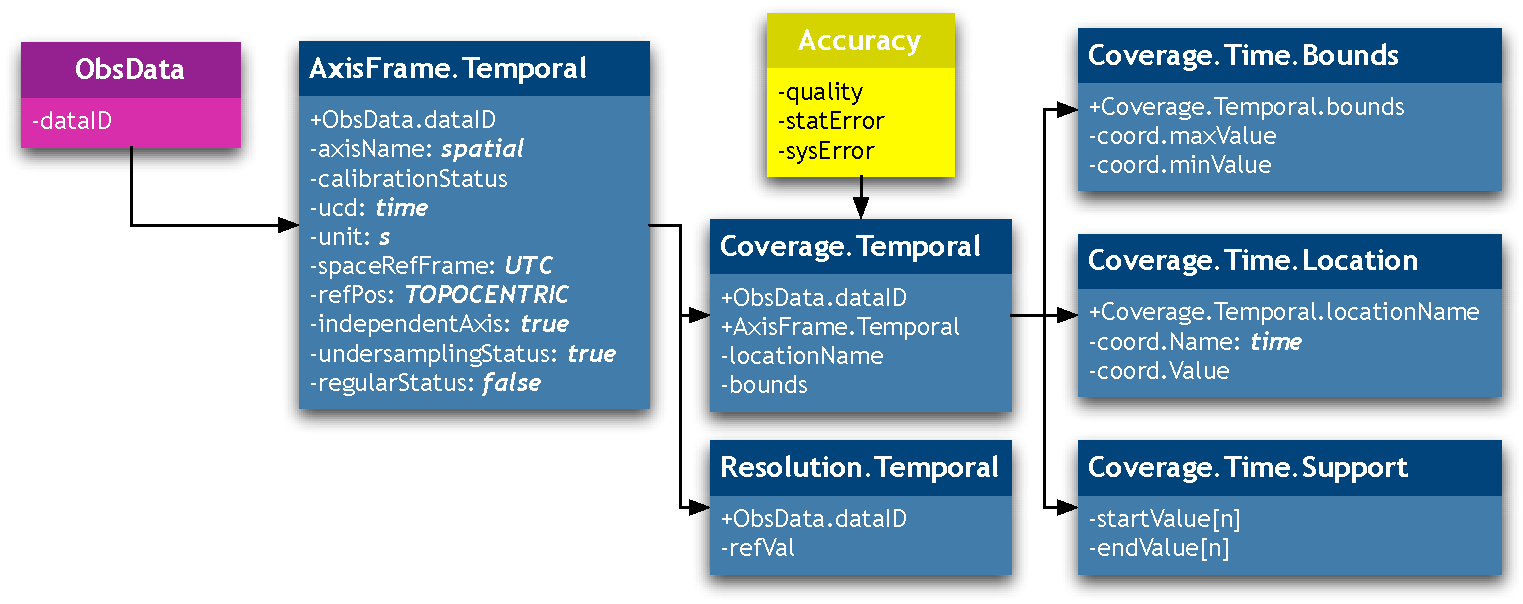
\includegraphics[width=\columnwidth]
				{fig/AxisFrame-Temporal-DM}
				\end{center}
				\caption[Temporal axis metadata]{
					Temporal axis and related coverage metadata.
				}
				\label{figAxisFrameTemporal}
			\end{figure}
			
			\begin{description}
				\item[AxisFrame.Temporal] Describes the 
				properties of the time axis, such as whether the
				axis is calibrated or not ({calibrationStatus}),
				units, reference system ({refPos}), time-scale
				({timescale}), whether the axis is sampled or not
				({undersamplingStatus}), and if sampled, whether
				sampling is regular or not ({samplingStatus}). In
				the case of spectroscopic data, time is not
				sampled.
				
				 We will use the {independentAxis} attribute to
				signal axis dependency as true for continuum
				observations.
				
				 \item[Coverage.Temporal] Collects all the temporal
				characterisation of the observational data.
				
				 \item[Coverage.Temporal.Location]
				Location instances hold the most representative
				value for each axis. For the temporal axis, it holds
				the time of observation, either the starting time
				or the time at the middle of the observation.
				
				 \item[Coverage.Temporal.Bounds] Bounds instances
				hold the maximum and minimum values for the axis.
				In the temporal axis, this is defined as the
				complete observation interval; alternatively, the
				total integration time can be used.
				
				 \item[Coverage.Temporal.Support] Coverage.Support
				instances provide the regions of an axis holding
				observational data. In the temporal axis, this are
				the time intervals actually devoted to flux
				collection\footnote{Actual execution time for each
				individual sub-scan.}.
				
				 \item[Coverage.Temporal.Sensitivity] In cases
				where an instrument had a sensor ramp-up, where
				some time is needed before 100\% sensitivity is
				achieved, this class would describe such a ramp,
				and would allow for convenient scaling of data
				taken during those intervals. If that were never
				the case, Temporal.Sensitivity could just be
				dropped.
				
				 \item[Resolution.Temporal] Holds the temporal
				resolution of the data. Most of the time, telescope
				control system time-stamps are expressed in UTC or
				LST in seconds, so temporal resolution would be of
				the order of a second, but normally the instrument
				could deliver better temporal resolution. We should
				address this after the initial setup.
				
				 We will not develop the SamplingPrecision.Temporal
				class, because we are not sampling the temporal
				axis.
				
				\item[Accuracy.Temporal] This class has to collect
				systematic and statistical errors associated with
				the temporal coordinates of the data. The Quality
				attribute gives additional information about the
				temporal data quality. We could use time re-syncing
				statistics in order to evaluate accuracy.
			\end{description}
			
			
			\begin{table}
			\begin{minipage}{\linewidth}
			\caption[AxisFrame.Temporal metadata]{AxisFrame.Temporal metadata.}
			\begin{smallertabular}{p{3.15 cm}p{1.5cm}p{2.25cm}p{4.35cm}}
						  & \textbf{FITS} & & \\ \textbf{Attribute} &
			              \textbf{Keyword} & \textbf{UCD} &
			              \textbf{Description}\\ \midrule axisName
			              & \texttt{assign} & \texttt{meta.id;
			              meta.main} & Axis name.\\ \addlinespace
			              calibrationStatus & \texttt{assign} &
			              \texttt{time; obs.calib; meta.code} &
			              Calibration status from a controlled
			              vocabulary: \texttt{un\-cal\-i\-brated},
			              \texttt{cal\-i\-brated},
			              \texttt{rel\-a\-tive}\footnote{\texttt{rel\-a\-tive}
			              refers to calibrated data, except for an
			              additive or multiplicative constant.} ,
			              \texttt{nor\-mal\-ized}\footnote{\texttt{normalized}
			              refers to dimensionless quantities, such as
			              those resulting from the division between two
			              commensurable datasets.} \\ \addlinespace ucd &
			              \texttt{assign} & \texttt{time; meta.ucd;
			              meta.main} & Main UCD for the axis.\\ \addlinespace
			              unit & \texttt{assign} & \texttt{time;
			              meta.unit; meta.main} & Main units for the
			              axis.\\ \addlinespace refPos & \texttt{assign} &
			              \texttt{time; meta.ref; meta.id} &
			              Identification of the origin position from a
			              controlled vocabulary.\\ \addlinespace
			              independentAxis & \texttt{assign} &
			              \texttt{time; obs.param; meta.code} & Boolean
			              flag indicating whether the axis is
			              independent of the rest or not.\\ \addlinespace
			              undersamplingStatus & \texttt{assign} &
			              \texttt{time; obs.param; meta.code} & Boolean
			              flag indicating whether the data are sampled
			              in this axis or not.\\ \addlinespace regularStatus &
			              \texttt{assign} & \texttt{time; obs.param;
			              meta.code} & Boolean flag used in case of
			              sampled data, indicating whether sampling is
			              regular or not.\\ \addlinespace numBins &
			              \texttt{assign} & \texttt{time; meta.number}
			              & Number of time samples.\\ \addlinespace
			\end{smallertabular}
			\label{tabAxisFrameTemporalMetadata}
			\end{minipage}
			\end{table}
			
			\begin{table}
			\caption[Coverage.Temporal.Location metadata]
			{Coverage.Temporal.Location metadata.}
			\begin{smallertabular}{p{2.15 cm}p{1.5cm}p{2.25cm}p{5.35cm}}
								& \textbf{FITS} & & \\ \textbf{Attribute} &
			                    \textbf{Keyword} & \textbf{UCD} &
			                    \textbf{Description}\\ \midrule coord.name &
			                    \texttt{assign} & \texttt{time; meta.name} & Name
			                    of the coordinate whose value goes in
			                    coord.value; in this case, \texttt{time} with
			                    respect to refPos. \\ \addlinespace coord.value &
			                    \texttt{assign} & \texttt{time; meta.number} &
			                    Numeric value for the time location; usually, a
			                    MJD or decimal UTC time. \\ \addlinespace
			\end{smallertabular}
			\label{tabCoverageTemporalLocationMetadata}
			\end{table}
			
			\begin{table}
			\begin{minipage}{\linewidth}
			\caption[Coverage.Temporal.Bounds metadata]
			{
					Coverage.Temporal.Bounds metadata\footnote{The UCDs for
			        coord.maxValue and coord.minValue could have been,
			        respectively, \texttt{time.obs.start} and
			        \texttt{time.obs.end}, but we think the proposed UCDs are more
			        consistent with the rest of the axes. Besides, we can defer the
			        election, by using \texttt{time.obs.start} and
			        \texttt{time.obs.end} at the beginning of the UCD, and
			        appending \texttt{meta.number; stat.max} or
			        \texttt{meta.number; stat.min} as additional qualifiers.}.
			}
			\begin{smallertabular}{p{2.15 cm}p{1.5cm}p{2.25cm}p{5.35cm}}
								& \textbf{FITS} & & \\ \textbf{Attribute} &
			                    \textbf{Keyword} & \textbf{UCD} &
			                    \textbf{Description}\\ \midrule coord.name &
			                    \texttt{assign} & \texttt{time; meta.name} & Name
			                    of the coordinate whose maximum and minimum
			                    values go in coord.maxValue and coord.minValue.\\
			                    \addlinespace coord.maxValue & \texttt{assign} &
			                    \texttt{time; meta.number; stat.max} & Minimum
			                    numeric value for the observation time.\\ \addlinespace
			                    coord.minValue & \texttt{assign} & \texttt{time;
			                    meta.number; stat.min} & Maximum numeric value
			                    for the observation time.\\ \addlinespace
			\end{smallertabular}
			\label{tabCoverageTemporalBoundsMetadata}
			\end{minipage}
			\end{table}
			
			\begin{table}
			\begin{minipage}{\linewidth}
			\caption[Coverage.Temporal.Support metadata]
			{
					Coverage.Temporal.Support
			        metadata\footnote{Coverage.Temporal.Support could be
			        alternatively defined by using just one value, the exposure
			        time, with UCD \texttt{time.expo}. The chosen definition, apart
			        from being more consistent across axes, allows for
			        discontinuous temporal support.}.
			}
			\begin{smallertabular}{p{2.15 cm}p{1.5cm}p{2.25cm}p{5.35cm}}
								& \textbf{FITS} & & \\ \textbf{Attribute} &
			                    \textbf{Keyword} & \textbf{UCD} &
			                    \textbf{Description}\\ \midrule code &
			                    \texttt{assign} & \texttt{time; meta.code} & Code
			                    for the time interval where we will be defining
			                    support; an array of [coord.code, startValue,
			                    endValue] tuples can be used to define temporal
			                    support.\\ \addlinespace startValue & \texttt{assign} &
			                    \texttt{time.expo.start} & Time interval start
			                    value.\\ \addlinespace endValue & \texttt{assign} &
			                    \texttt{time.expo.end} & 2DTime interval end
			                    value.\\ \addlinespace
			\end{smallertabular}
			\label{tabCoverageTemporalSupportMetadata}
			\end{minipage}
			\end{table}
			
			\begin{table}
			\caption[Coverage.Temporal.Resolution metadata]
			{Coverage.Temporal.Resolution metadata.}
			\begin{smallertabular}{p{2.15 cm}p{1.5cm}p{2.25cm}p{5.35cm}}
								& \textbf{FITS} & & \\ \textbf{Attribute} &
			                    \textbf{Keyword} & \textbf{UCD} &
			                    \textbf{Description}\\ \midrule
			                    referenceValue & \texttt{assign} & \texttt{time;
			                    meta.number; meta.ref} & Resolution reference
			                    value.\\ \addlinespace
			\end{smallertabular}
			\label{tabCoverageTemporalResolutionMetadata}
			\end{table}
			
			\begin{table}
			\caption[Accuracy.Temporal metadata]{Accuracy.Temporal metadata.}
			\begin{smallertabular}{p{2.15 cm}p{1.5cm}p{2.25cm}p{5.35cm}}
								& \textbf{FITS} & & \\ \textbf{Attribute} &
			                    \textbf{Keyword} & \textbf{UCD} &
			                    \textbf{Description}\\ \midrule quality &
			                    \texttt{assign} & \texttt{time; meta.code.qual} &
			                    Quality code for time coordinates; invalid data
			                    are flagged with a quality code of 1.\\ \addlinespace
			                    sysError & \texttt{assign} & \texttt{time;
			                    stat.error.sys} & Systematic error for time
			                    coordinates.\\ \addlinespace sysErrorHigh &
			                    \texttt{assign} & \texttt{time; stat.error.sys;
			                    stat.max} & Maximum systematic error for time
			                    coordinates.\\ \addlinespace sysErrorLow &
			                    \texttt{assign} & \texttt{time; stat.error.sys;
			                    stat.min} & Minimum systematic error for time
			                    coordinates.\\ \addlinespace statError & \texttt{assign}
			                    & \texttt{time; stat.error} & Statistical error
			                    for time coordinates.\\ \addlinespace statErrorHigh&
			                    \texttt{assign} & \texttt{time; stat.error;
			                    stat.max} & Maximum statistical error for time
			                    coordinates.\\ \addlinespace statErrorLow &
			                    \texttt{assign} & \texttt{time; stat.error;
			                    stat.min} & Minimum statistical error for time
			                    coordinates.\\ \addlinespace
			\end{smallertabular}
			\label{tabAccuracyTemporalMetadata}
			\end{table}
			
		% subsection ssubTemporalAxis (end)
		
		\subsection{AxisFrame.Spectral and Coverage.Spectral} %(fold)
		\label{subSpectralAxis}
			
			In this subsection, we describe the classes that
			configure the description of the spectral axis
			(AxisFrame.Spectral), and the characterisation of the
			coverage in such axis (Coverage.Spectral).
			Figure~\ref{figAxisFrameSpectral} shows the classes and
			their relationships.
			
			\begin{figure}[tbp]
			\begin{center}
			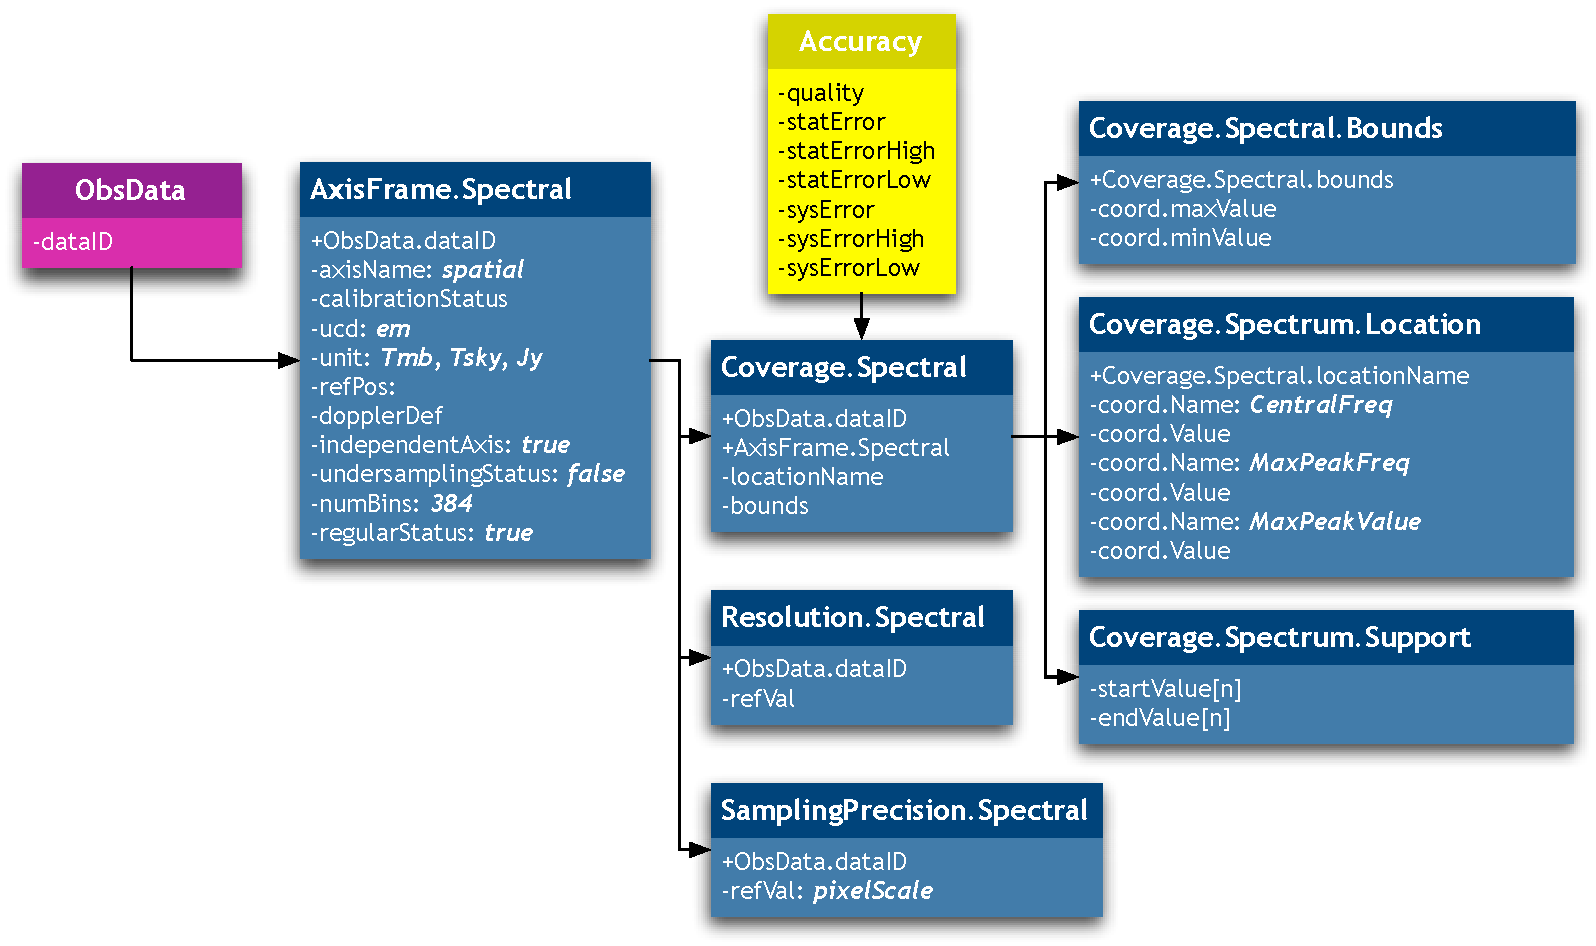
\includegraphics[width=\columnwidth]
			{fig/AxisFrame-Spectral-DM}
			\end{center}
			\caption[Spectral axis metadata]{
				Spectral axis and related coverage metadata.
			}
			\label{figAxisFrameSpectral}
			\end{figure}

			\begin{description}
				\item[AxisFrame.Spectral] Describes the 
				properties of the spectral axis, such as whether the
				axis is calibrated or not (calibrationStatus),
				units, reference system (RefPos), or the
				mathematical definition used for the Doppler effect
				(DopplerDef), for velocity calibrated
				spectra\footnote{For systems in the local standard
				of rest (LSR), emission lines occur at a precise
				frequency. Due do the Doppler effect, systems
				receding from the LSR will show a lower frequency,
				and those approaching will show higher frequencies.
				In the case of complex dynamics, the net effect is
				a broadening of the line, and the Doppler effect
				allows us to calibrate emission at different
				frequencies as emission at different velocities.}.
				It is clear that spectral information is indeed
				sampled, and the number of channels will be coded
				by numBins.
				
				 \item[Coverage.Spectral] Collects the different
				spectral properties of the data.
				
				 \item[Coverage.Spectral.Location]
				Coverage.Location holds the most representative
				value for the axis. In the spectral axis, and being
				a sampled axis, we will use the frequency for the
				central sample of the spectrum.
				
				 \item[Coverage.Spectral.Bounds] Holds the spectral
				limits of the data, that is, the starting and
				ending frequency for the spectrum.
				
				 \item[Coverage.Spectral.Support] Holds the
				spectral support for the data. We could choose to
				register just the actual bandwidth, or better, to
				set an array of different intervals where the
				instrument is sensitive. Better yet, we could
				register a sensitivity profile for each frequency.
				We will initially choose the array of intervals as
				the way to express the spectral support.
				
				 \item[Coverage.Spectral.Sensitivity] Holds the
				sensitivity profile for the instrument in
				frequency; in other words, this would be equal to
				the detailed frequency response of the whole
				antenna-receiver-backend set.
				
				 \item[Resolution.Spectral] Holds the spectral
				resolution information for the data. For filter
				banks, it is the filter bandwidth for each filter,
				or an average filter bandwidth. In the case of
				spectra obtained from the Fourier transform of the
				autocorrelation function, it is equal to the
				bandwidth divided by the number of channels.
				
				 \item[SamplingPrecision.Spectral] In the case of
				the Robledo antenna, this value should be equal to
				the value stored at Resolution.Spectral. For other
				instruments, SamplingPrecision.Spectral defines the
				frequency steps from one frequency bin to the next.
				
				 \item[Accuracy.Spectral] Errors associated with
				the spectrum. In the same way as the support could
				change along the spectrum, because of different
				sensitivities, we might need to characterise the
				accuracy along the spectrum. At least in the case
				of Robledo, the SNR is global, and considered equal
				for all frequencies. If not, a first approximation
				can be using an average SNR, and maximum and
				minimum SNR.
			\end{description}
			
			\begin{table}
			\begin{minipage}{\linewidth}
			\caption[AxisFrame.Spectral metadata]{AxisFrame.Spectral metadata.}
			\begin{smallertabular}{p{3.05 cm}p{1.5cm}p{2.85cm}p{3.85cm}}
							& \textbf{FITS} & & \\ \textbf{Attribute} &
			                \textbf{Keyword} & \textbf{UCD} &
			                \textbf{Description}\\ \midrule axisName &
			                \texttt{assign} & \texttt{meta.id; meta.main} & Axis
			                name (\texttt{frequency} or \texttt{velocity}).\\
			                \addlinespace calibrationStatus & \texttt{assign} &
			                \texttt{em.radio; obs.calib; meta.code} & Calibration
			                status from a controlled vocabulary:
			                \texttt{un\-cal\-i\-brated}, \texttt{cal\-i\-brated},
			                \texttt{rel\-a\-tive}\footnote{\texttt{rel\-a\-tive}
			                refers to calibrated data, except for an additive or
			                multiplicative constant} ,
			                \texttt{nor\-mal\-ized}\footnote{\texttt{normalized}
			                refers to dimensionless quantities, such as those
			                resulting from the division between two commensurable
			                datasets.}.\\ \addlinespace ucd & \texttt{assign} &
			                \texttt{em.radio; meta.ucd; meta.main} & Main UCD for
			                the axis.\\ \addlinespace unit & \texttt{TUNITn} &
			                \texttt{em.radio; meta.unit; meta.main} & Main units
			                for the axis.\\ \addlinespace refPos & \texttt{assign} &
			                \texttt{em.radio; meta.ref; meta.id} & Identification
			                of the origin position from a controlled
			                vocabulary.\\ \addlinespace dopplerDef & \texttt{VELDEF} &
			                \texttt{spect.dopplerParam; meta.code} & Code
			                defining the type of Doppler shift definition used
			                for frequency and/or velocity calibration; from a
			                controlled vocabulary: \texttt{op\-ti\-cal},
			                \texttt{ra\-di\-o}, \texttt{rel\-a\-tiv\-is\-tic}.\\
			                \addlinespace independentAxis & \texttt{assign} &
			                \texttt{em.radio; obs.param; meta.code} & Boolean
			                flag indicating whether the axis is independent of
			                the rest or not.\\ \addlinespace undersamplingStatus &
			                \texttt{assign} & \texttt{em.radio; obs.param;
			                meta.code} & Boolean flag indicating whether the data
			                are sampled in this axis or not.\\ \addlinespace
			                regularStatus & \texttt{assign} & \texttt{em.radio;
			                obs.param; meta.code} & Boolean flag used in case of
			                sampled data, indicating whether sampling is regular
			                or not.\\ \addlinespace numBins & \texttt{assign} &
			                \texttt{em.radio; meta.number} & Number of spectral
			                samples.\\ \addlinespace
			\end{smallertabular}
			\label{tabAxisFrameSpectralMetadata}
			\end{minipage}
			\end{table}
			
			\begin{table}
			\caption[Coverage.Spectral.Location metadata]
			{Coverage.Spectral.Location metadata.}
			\begin{smallertabular}{p{2.15 cm}p{1.5cm}p{2.25cm}p{5.35cm}}
						& \textbf{FITS} & & \\ \textbf{Attribute} &
			            \textbf{Keyword} & \textbf{UCD} & \textbf{Description}\\
			            \midrule coord.name & \texttt{assign} &
			            \texttt{em.radio; meta.name} & Name of the coordinate
			            whose value goes in coord.value; in this case,
			            \texttt{frequency} with respect to refPos.\\ \addlinespace
			            coord.value & \texttt{OBSFREQ} & \texttt{em.radio;
			            em.freq; stat.mean} & Numeric value for the central
			            frequency location.\\ \addlinespace
			\end{smallertabular}
			\label{tabCoverageSpectralLocationMetadata}
			\end{table}
			
			\begin{table}
			\caption[Coverage.Spectral.Bounds metadata]
			{Coverage.Spectral.Bounds metadata.}
			\begin{smallertabular}{p{2.15 cm}p{1.5cm}p{2.25cm}p{5.35cm}}
						& \textbf{FITS} & & \\ \textbf{Attribute} &
			            \textbf{Keyword} & \textbf{UCD} & \textbf{Description}\\
			            \midrule coord.name & \texttt{assign} &
			            \texttt{em.radio; meta.name} & Name of the coordinate
			            whose maximum and minimum values go in coord.maxValue and
			            coord.minValue.\\ \addlinespace coord.maxValue & \texttt{assign}
			            & \texttt{em.freq; meta.number; stat.max} & Minimum
			            frequency value.\\ \addlinespace coord.minValue &
			            \texttt{assign} & \texttt{em.freq; meta.number; stat.min}
			            & Maximum frequency value.\\ \addlinespace
			\end{smallertabular}
			\label{tabCoverageSpectralBoundsMetadata}
			\end{table}
			
			\begin{table}
			\caption[Coverage.Spectral.Support metadata]
			{Coverage.Spectral.Support metadata.}
			\begin{smallertabular}{p{2.15 cm}p{1.5cm}p{2.25cm}p{5.35cm}}
						& \textbf{FITS} & & \\ \textbf{Attribute} &
			            \textbf{Keyword} & \textbf{UCD} & \textbf{Description}\\
			            \midrule code & \texttt{assign} & \texttt{em.radio;
			            meta.record} & Code for the interval where we will be
			            defining support; an array of [coord.code, startValue,
			            endValue] tuples can be used to define spectral support.\\
			            \addlinespace startValue & \texttt{assign} & \texttt{em.freq;
			            stat.min} & Frequency interval start value.\\ \addlinespace
			            endValue & \texttt{assign} & \texttt{em.freq; stat.max} &
			            Frequency interval end value.\\ \addlinespace
			\end{smallertabular}
			\label{tabCoverageSpectralSupportMetadata}
			\end{table}
			
			\begin{table}
			\caption[Coverage.Spectral.Sensitivity metadata]
			{Coverage.Spectral.Sensitivity metadata.}
			\begin{smallertabular}{p{2.15 cm}p{1.5cm}p{2.25cm}p{5.35cm}}
						& \textbf{FITS} & & \\ \textbf{Attribute} &
			            \textbf{Keyword} & \textbf{UCD} & \textbf{Description}\\
			            \midrule numChannels & \texttt{assign} &
			            \texttt{em.radio; meta.number} & Number of channels of
			            the frequency response of the filter that describes
			            spectral sensitivity.\\ \addlinespace channel[n] &
			            \texttt{assign} & \texttt{em.freq} & Frequency for the
			            n\thsup{} channel of the filter that describes spectral
			            sensitivity.\\ \addlinespace response[n] & \texttt{assign} &
			            \texttt{arith.factor} & Filter response for the n\thsup{}
			            channel.\\ \addlinespace
			\end{smallertabular}
			\label{tabCoverageSpectralSensitivityMetadata}
			\end{table}
			
			\begin{table}
			\begin{minipage}{\linewidth}
			\caption[Coverage.Spectral.Resolution metadata]
			{Coverage.Spectral.Resolution metadata\footnote{When the Sensitivity
			class is provided, Resolution.numChannels has to be equal to
			Sensitivity.numChannels, and each channel can support different
			resolutions. When the Sensitivity class is not provided,
			Resolution.numChannels has to be set to \texttt{1}, and
			Resolution.referenceValue represents the average channel
			resolution.}.}
			\begin{smallertabular}{p{2.15 cm}p{1.5cm}p{2.45cm}p{5.15cm}}
						& \textbf{FITS} & & \\ \textbf{Attribute} &
			            \textbf{Keyword} & \textbf{UCD} & \textbf{Description}\\
			            \midrule numChannels & \texttt{assign} &
			            \texttt{em.radio; meta.number} & Number of channels for
			            which resolution is provided.\\ \addlinespace referenceValue[n]
			            & \texttt{FREQRES} & \texttt{em.freq; spect.resolution} &
			            Resolution reference value for the n\thsup{} channel.\\ \addlinespace
			\end{smallertabular}
			\label{tabCoverageSpectralResolutionMetadata}
			\end{minipage}
			\end{table}
			
			\begin{table}
			\begin{minipage}{\linewidth}
			\caption[SamplingPrecision.Spectral metadata]
			{SamplingPrecision.Spectral metadata\footnote{When
			SamplingPrecision.numChannels is set to \texttt{0}, the number of
			spectral channels is given by AxisFrame.Spectral.numBins, and
			SamplingPrecision provides the sampling step in a single
			referenceValue. Otherwise, SamplingPrecision.Spectral.numBins must be
			equal to AxisFrame.Spectral.numBins, and when the Sensitivity class
			is provided, SamplingPrecision.Spectral.numBins must be equal to
			Spectral.Sensitivity.numChannels, and
			Spectral.SamplingPrecision.referenceValue[n] equal to
			Spectral.Sensitivity.channel[n].}.}
			\begin{smallertabular}{p{2.15 cm}p{1.5cm}p{2.45cm}p{5.15cm}}
						& \textbf{FITS} & & \\ \textbf{Attribute} &
			            \textbf{Keyword} & \textbf{UCD} & \textbf{Description}\\
			            \midrule numChannels & \texttt{assign} &
			            \texttt{em.radio; meta.number} & Number of frequencies
			            that we are sampling.\\ \addlinespace referenceValue[n] &
			            \texttt{FREQRES} & \texttt{em.freq; spect.resolution} &
			            Resolution reference value for the n\thsup{} channel.\\ \addlinespace
			\end{smallertabular}
			\label{tabSamplingPrecisionSpectralMetadata}
			\end{minipage}
			\end{table}
			
			\begin{table}
			\caption[Accuracy.Spectral metadata]{Accuracy.Spectral metadata.}
			\begin{smallertabular}{p{2.15 cm}p{1.5cm}p{2.25cm}p{5.35cm}}
						& \textbf{FITS} & & \\ \textbf{Attribute} &
			            \textbf{Keyword} & \textbf{UCD} & \textbf{Description}\\
			            \midrule quality & \texttt{assign} &
			            \texttt{em.freq; meta.code.qual} &Quality code for
			            frequency coordinates; invalid data are flagged with a
			            quality code of 1.\\ \addlinespace sysError & \texttt{assign} &
			            \texttt{em.freq; stat.error.sys} &Systematic error for
			            frequency coordinates.\\ \addlinespace sysErrorHigh &
			            \texttt{assign} & \texttt{em.freq; stat.error.sys;
			            stat.max} & Maximum systematic error for frequency
			            coordinates.\\ \addlinespace sysErrorLow & \texttt{assign} &
			            \texttt{em.freq; stat.error.sys; stat.min} & Minimum
			            systematic error for frequency coordinates.\\ \addlinespace
			            statError & \texttt{assign} & \texttt{em.freq;
			            stat.error} &Statistical error for frequency
			            coordinates.\\ \addlinespace statErrorHigh& \texttt{assign} &
			            \texttt{em.freq; stat.error; stat.max} & Maximum
			            statistical error for frequency coordinates.\\ \addlinespace
			            statErrorLow & \texttt{assign} & \texttt{em.freq;
			            stat.error; stat.min} & Minimum statistical error for
			            frequency coordinates.\\ \addlinespace
			\end{smallertabular}
			\label{tabAccuracySpectralMetadata}
			\end{table}
			
		% subsection subSpectralAxis (end)

		\subsection{AxisFrame.Observable and Coverage.Observable} %(fold)
		\label{ssubObservableAxis}
			
			The Observable axis is, finally, the one directly
			related to the stored data, instead of data headers. In
			this subsection, we describe the classes that configure
			the description of the observable axis
			(AxisFrame.Observable), and the characterisation of the
			coverage in such axis (Coverage.Observable).
			Figure~\ref{figAxisFrameObservable} shows the classes
			and their relationships.
			
			\begin{figure}[tbp]
			\begin{center}
				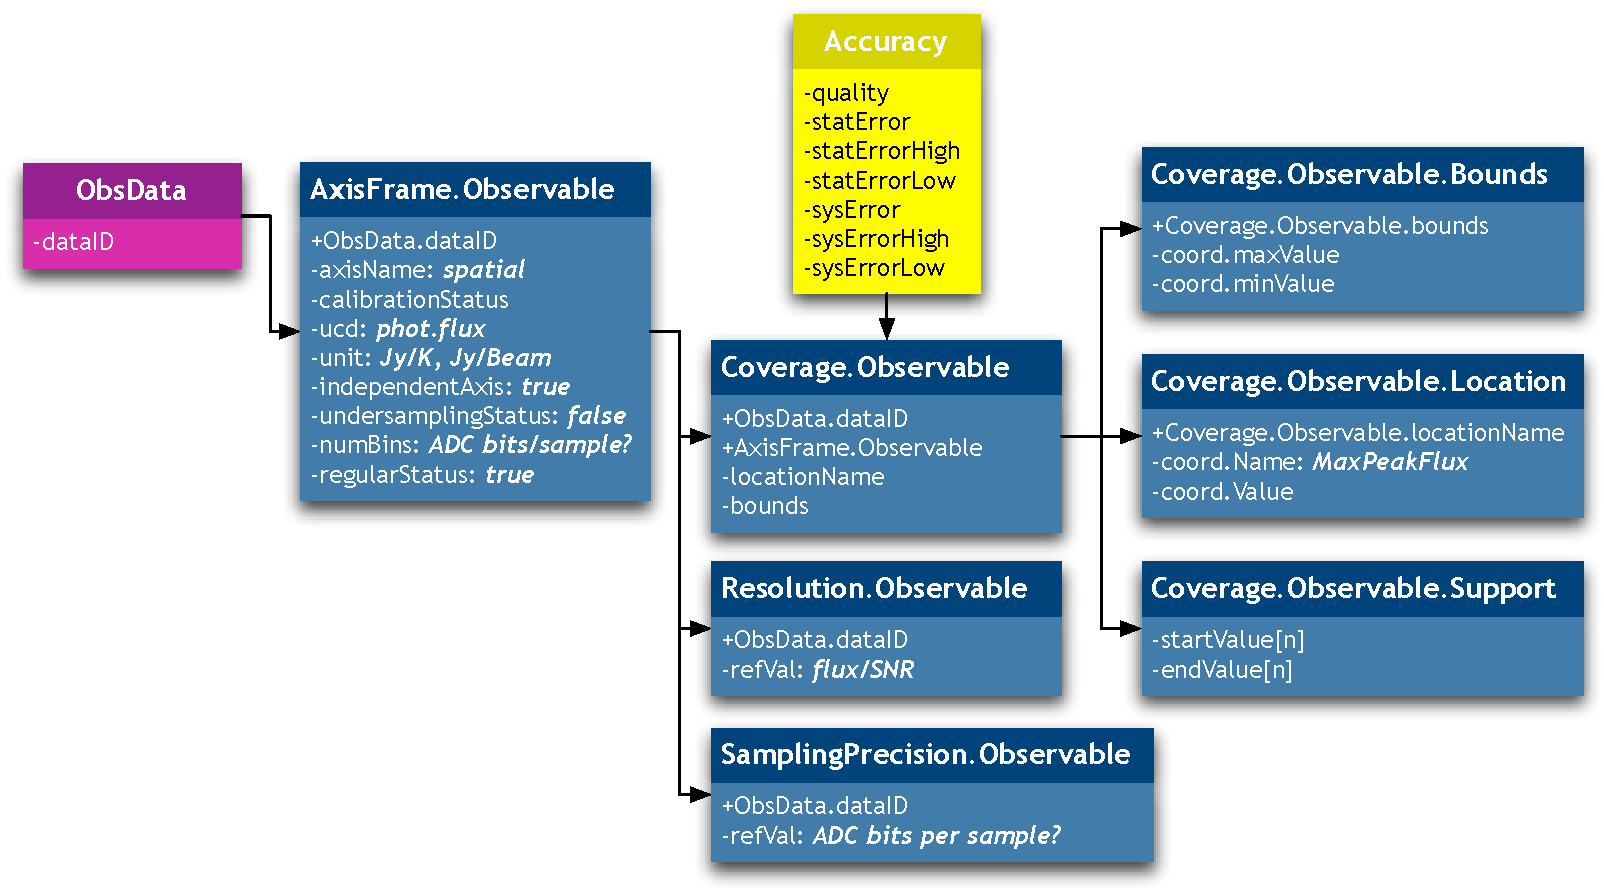
\includegraphics[width=\columnwidth]
				{fig/AxisFrame-Observable-DM}
			\end{center}
			\caption[Observable axis metadata]
			{Observable axis and related coverage metadata.}
			\label{figAxisFrameObservable}
			\end{figure}

			\begin{description}
				\item[AxisFrame.Observable] Describes the 
				properties of the observable axis (whether the
				observable is flux,
				polarisation state, or any other), such as whether
				the data is calibrated or not (calibrationStatus),
				applicable units, et cetera. Flux information is
				sampled at the digital conversion stage, and the
				number of available different flux levels is
				codified in numBins. By specifying units in this
				class, we define whether the observable data are
				provided in flux units, or in brightness or antenna
				temperature. Additional information, such as the
				polarisation, can be accommodated in the same axis
				in the same way we extended the Spatial axis for 2D
				or 3D coordinates, or by means of (an) additional
				observable (axis) axes.
				
				 \item[Coverage.Observable] Collects all
				information that directly characterises observable
				data.
				
				 \item[Coverage.Observable.Location]
				Coverage.Location instances hold the most
				representative value for that axis. In this case,
				the average spectrum flux is not significant,
				specially if we have a strong line detection.
				Hence, for this axis we will take the maximum flux
				as Observable.Location.
				
				 \item[Coverage.Observable.Bounds] Coverage.Bounds
				instances record the maximum and minimum values for
				the axis. In the Observable axis, it records
				minimum and maximum flux for the spectrum.
				
				 \item[Coverage.Observable.Support] This instance
				should give us the intervals of flux observed in
				the spectrum, and we could choose between making it
				equal to Coverage.Observable.Bounds, or defining an
				interval that holds a given dispersion from the
				Coverage.Observable.Location value. We will
				initially consider Coverage.Observable.Support as
				equal to Coverage.Observable.Bounds.
				
				 \item[Coverage.Observable.Sensitivity] This would
				store the change rate in the observable axis for a
				given observed flux.
				
				 \item[Resolution.Observable] We keep the flux
				resolution for the data, defined as mean flux
				divided by the SNR, or mean noise.
				
				 \item[SamplingPrecision.Observable] Instances of
				this class indicate the sampling precision. For the
				observable (flux) axis, this should be equal to the
				Analog to Digital Converter (ADC) resolution, or
				worse if more processing is involved, and should be
				tabulated by instrument setup. We might also
				consider this axis as non-sampled, as
				Resolution.Observable is usually well above ADC
				resolution, and drop this class.
				
				 \item[Accuracy.Observable] Collected flux
				associated errors. Errors on the observable axis
				can be dependent on received flux, and so we should
				give an average value, and either variance or
				maximum and minimum accuracy on the observable
				axis.
				
				 If the observable variable were a different one,
				the main difference would correspond to the change
				of UCDs. In the particular case of polarisation,
				\texttt{phot.flux} would be replaced by
				\texttt{phys.polarization}. Other changes would
				include an additional characterisation of the
				parameters been actually returned by the
				instrument, and their relationship with Stokes
				parameters.
			\end{description}
			
			\begin{table}
			\begin{minipage}{\linewidth}
			\caption[AxisFrame.Observable metadata]
			{AxisFrame.Observable metadata (when the observed variable is flux).}
			\begin{smallertabular}{p{3.15 cm}p{1.5cm}p{2.25cm}p{4.35cm}}
						& \textbf{FITS} & & \\ \textbf{Attribute} &
			            \textbf{Keyword} & \textbf{UCD} & \textbf{Description}\\
			            \midrule axisName & \texttt{assign} &
			            \texttt{meta.id; meta.main} & Axis name.\\ \addlinespace
			            calibrationStatus & \texttt{assign} & \texttt{em.radio;
			            obs.calib; meta.code} & Calibration status from a
			            controlled vocabulary: \texttt{un\-cal\-i\-brated},
			            \texttt{cal\-i\-brated},
			            \texttt{rel\-a\-tive}\footnote{\texttt{rel\-a\-tive}
			            refers to calibrated data, except for an additive or
			            multiplicative constant} ,
			            \texttt{nor\-mal\-ized}\footnote{\texttt{nor\-ma\-lized}
			            refers to dimensionless quantities, such as those
			            resulting from the division between two commensurable
			            datasets.}.\\ \addlinespace ucd & \texttt{assign} &
			            \texttt{phot.flux; meta.ucd; meta.main} & Main UCD for
			            the axis.\\ \addlinespace unit & \texttt{TUNITn} &
			            \texttt{phot.flux; meta.unit; meta.main} & Main units for
			            the axis.\\ \addlinespace refPos & \texttt{assign} &
			            \texttt{phot.flux; meta.ref; meta.id} & Identification of
			            the origin position from a controlled vocabulary.\\
			            \addlinespace independentAxis & \texttt{assign} &
			            \texttt{phot.flux; obs.param; meta.code} & Boolean flag
			            indicating whether the axis is independent of the rest or
			            not.\\ \addlinespace undersamplingStatus & \texttt{assign} &
			            \texttt{phot.flux; obs.param; meta.code} & Boolean flag
			            indicating whether the data are sampled in this axis or
			            not.\\ \addlinespace regularStatus & \texttt{assign} &
			            \texttt{phot.flux; obs.param; meta.code} & Boolean flag
			            used in case of sampled data, indicating whether sampling
			            is regular or not.\\ \addlinespace numBins & \texttt{assign} &
			            \texttt{phot.flux; meta.number} & Number of spectral
			            samples (if the axis is sampled)\\ \addlinespace
			\end{smallertabular}
			\label{tabAxisFrameObservableMetadata}
			\end{minipage}
			\end{table}
			
			\begin{table}
			\caption[Coverage.Observable.Location metadata]
			{Coverage.Observable.Location metadata (when the observed variable is
			flux).}
			\begin{smallertabular}{p{2.15 cm}p{1.5cm}p{2.25cm}p{5.35cm}}
						& \textbf{FITS} & & \\ \textbf{Attribute} &
			            \textbf{Keyword} & \textbf{UCD} & \textbf{Description}\\
			            \midrule coord.name & \texttt{assign} &
			            \texttt{phot.flux; meta.name} & Name of the coordinate
			            whose value goes in coord.value; in this case,
			            \texttt{flux} with respect to refPos.\\ \addlinespace
			            coord.value & \texttt{assign} & \texttt{phot.flux;
			            stat.max} & Numeric value for the maximum flux (flux
			            location).\\ \addlinespace
			\end{smallertabular}
			\label{tabCoverageObservableLocationMetadata}
			\end{table}
			
			\begin{table}
			\caption[Coverage.Observable.Bounds metadata]
			{Coverage.Observable.Bounds metadata.}
			\begin{smallertabular}{p{2.15 cm}p{1.5cm}p{2.25cm}p{5.35cm}}
						& \textbf{FITS} & & \\ \textbf{Attribute} &
			            \textbf{Keyword} & \textbf{UCD} & \textbf{Description}\\
			            \midrule coord.name & \texttt{assign} &
			            \texttt{phot.flux; meta.name} & Name of the coordinate
			            whose maximum and minimum values go in coord.maxValue and
			            coord.minValue.\\ \addlinespace coord.maxValue & \texttt{assign}
			            & \texttt{phot.flux; stat.max} & Minimum flux value.\\
			            \addlinespace coord.minValue & \texttt{assign} &
			            \texttt{phot.flux; stat.min} & Maximum flux value.\\
			            \addlinespace
			\end{smallertabular}
			\label{tabCoverageObservableBoundsMetadata}
			\end{table}
			
			\begin{table}
			\caption[Coverage.Observable.Support metadata]
			{Coverage.Observable.Support metadata
			(when the observed variable is flux).}
			\begin{smallertabular}{p{2.15 cm}p{1.5cm}p{2.25cm}p{5.35cm}}
						& \textbf{FITS} & & \\ \textbf{Attribute} &
			            \textbf{Keyword} & \textbf{UCD} & \textbf{Description}\\
			            \midrule code & \texttt{assign} & \texttt{em.radio;
			            meta.record} & Code for the interval where we will be
			            defining support; an array of [coord.code, startValue,
			            endValue] tuples can be used to define spectral support.\\
			            \addlinespace startValue & \texttt{assign} & \texttt{em.freq;
			            stat.min} & Frequency interval start value.\\ \addlinespace
			            endValue & \texttt{assign} & \texttt{em.freq; stat.max} &
			            Frequency interval end value.\\ \addlinespace
			\end{smallertabular}
			\label{tabCoverageObservableSupportMetadata}
			\end{table}
			
			%\begin{table}
			%\caption[Coverage.Observable.Sensitivity metadata]
			%{Coverage.Observable.Sensitivity metadata.}
			%\begin{smallertabular}{p{2.15 cm}p{1.5cm}p{2.25cm}p{5.35cm}}
			%			& \textbf{FITS} & & \\ \textbf{Attribute} &
			%            \textbf{Keyword} & \textbf{UCD} & \textbf{Description}\\
			%            \hline \hline
			%\end{smallertabular}
			%\label{tabCoverageObservableSensitivityMetadata}
			%\end{table}
			
			\begin{table}
			\caption[Coverage.Observable.Resolution metadata]
			{Coverage.Observable.Resolution metadata.}
			\begin{smallertabular}{p{2.15 cm}p{1.5cm}p{2.25cm}p{5.35cm}}
						& \textbf{FITS} & & \\ \textbf{Attribute} &
			            \textbf{Keyword} & \textbf{UCD} & \textbf{Description}\\
			            \midrule referenceValue & \texttt{assign} &
			            \texttt{phot.flux; stat.snr; arith.ratio} & Flux
			            resolution (Flux/SNR), as $$\mathrm{\frac{Flux}{SNR} =
			            flux \times \frac{fluxNoise}{fluxSignal}}.$$ Equivalent
			            to average noise.\\ \addlinespace
			\end{smallertabular}
			\label{tabCoverageObservableResolutionMetadata}
			\end{table}
			
			\begin{table}
			\begin{minipage}{\linewidth}
			\caption[SamplingPrecision.Observable metadata]
			{SamplingPrecision.Observable metadata\footnote{Somewhat redundant,
			given the presence of AxisFrame.Observable.numBins. However, we
			include it for completeness.}.}
			\begin{smallertabular}{p{2.15 cm}p{1.5cm}p{2.25cm}p{5.35cm}}
						& \textbf{FITS} & & \\ \textbf{Attribute} &
			            \textbf{Keyword} & \textbf{UCD} & \textbf{Description}\\
			            \midrule referenceValue & \texttt{assign} &
			            \texttt{phot.flux; instr.precision} & Flux sampling
			            precision; maybe expressed as the number of bits per
			            sample.\\ \addlinespace
			\end{smallertabular}
			\label{tabSamplingPrecisionObservableMetadata}
			\end{minipage}
			\end{table}
			
			\begin{table}
			\caption[Accuracy.Observable metadata]{Accuracy.Observable metadata.}
			\begin{smallertabular}{p{2.15 cm}p{1.5cm}p{2.25cm}p{5.35cm}}
						& \textbf{FITS} & & \\ \textbf{Attribute} &
			            \textbf{Keyword} & \textbf{UCD} & \textbf{Description}\\
			            \midrule quality & \texttt{assign} &
			            \texttt{phot.flux; meta.code.qual} &Quality code for the
			            observed flux; invalid data are flagged with a quality
			            code of 1.\\ \addlinespace sysError & \texttt{assign} &
			            \texttt{phot.flux; stat.error.sys} &Systematic error for
			            the observed flux.\\ \addlinespace sysErrorHigh &
			            \texttt{assign} & \texttt{phot.flux; stat.error.sys;
			            stat.max} & Maximum systematic error for the observed
			            flux.\\ \addlinespace sysErrorLow & \texttt{assign} &
			            \texttt{phot.flux; stat.error.sys; stat.min} & Minimum
			            systematic error for the observed flux.\\ \addlinespace
			            statError & \texttt{assign} & \texttt{phot.flux;
			            stat.error} &Statistical error for the observed flux.\\
			            \addlinespace statErrorHigh& \texttt{assign} &
			            \texttt{phot.flux; stat.error; stat.max} & Maximum
			            statistical error for the observed flux.\\ \addlinespace
			            statErrorLow & \texttt{assign} & \texttt{phot.flux;
			            stat.error; stat.min} & Minimum statistical error for the
			            observed flux.\\ \addlinespace
			\end{smallertabular}
			\label{tabAccuracyObservableMetadata}
			\end{table}
			
		% subsection ssubObservableAxis (end)

	% section subObsDataCharacterisation (end)


	\section{Target} % (fold)
	\label{subTargetDesc}
		\attributedquote{
			\dictionarydef
				{target}
				{noun}
				{
					\begin{itemize}
						\item a person, object, or place selected as
						the aim of an attack.
						
						\item a mark or point at which someone fires
						or aims, especially a round or rectangular 
						board marked with concentric circles used in
						archery or shooting.
					\end{itemize}
				}
				\dictionarydef
					{on target}
					{phrase}
					{
						\begin{itemize}
							\item accurately hitting the thing
							aimed at.
						\end{itemize}
					}
		}
		{The New  Oxford American Dictionary, \emph{2nd Edition}}
		
		
		\noindent
		It is necessary to have a systematic storage of the targets
		being studied, because we have to allow queries by
		previously studied targets, as it is very likely that
		this query will be the most used one.
		
		\begin{figure}[tbp]
			\begin{center}
				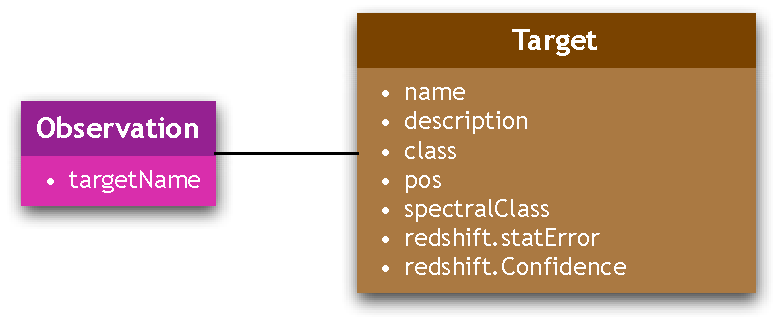
\includegraphics[width=0.5\columnwidth]
				{fig/Target-DM}
			\end{center}
			\caption[Target data model]{Target data model.}
			\label{figTargetDataModel}
		\end{figure}

		The ObsDM distinguishes between
		several types of targets:

		\begin{description}
			\item[Astronomical object] It is a target for which
			some properties are known before the observation.
			
			 \item[Source] An entity created after analysing an
			observation; represents the actual detection by an
			instrument.
			
			 \item[Field] A region of the sky, not a single point
			or collection of points.
			
			 \item[Pointing target] A particular location for an
			observation. It can be part of an Astronomical object,
			a Field, or other entities, such as a Calibrator.
		\end{description}

		IVOA has not developed the Target class as a whole, but the
		authors of the SDM~\cite{McDowell:2006fk} have developed a
		set of possible metadata. We will initially adopt that set
		for the RADAMS, and we can see the associated metadata in
		Figure~\ref{figTargetDataModel}.
		
		Another data model dealing with Targets is the Resource
		Data Model~\cite{2004ASPC..314..273H}, which considers
		additional targets for observations, such as radio flux
		calibrators, pointing calibrators, et cetera.
		
		We have to take into account that most of the time the
		archive will store ObsData associated to Pointing targets,
		but said Pointing targets can also be related to
		Astronomical Objects.
		\invisiblenote{E.g., in the scientific case we
		mentioned in section~\ref{subScientificCase}, the dish is
		pointed to a Pointing target in order to find a maser, but
		that Pointing target will be most likely included within an
		Astronomical object, such as a planetary nebula.}
		For instance, an astronomer might have a program in which
		s/he is looking for water masers as tracers of shocked
		regions, and specifies several Pointing targets. Those
		Pointing targets, however, will be most likely found within
		an Astronomical object, such as a planetary nebula. The
		association of the Astronomical object and the Pointing
		target will be made by means of the Target class.
		
	% section subTargetDesc (end)
	
	
	\section{Conclusions} % (fold)
	\label{sec:radams_cha_conclusions}
		
		In this chapter we have shown that the already specified
		IVOA data models for Characterisation, together with the
		Target data model, do not need to be altered in order to
		be used for radio astronomical archives.
		
		However, the UCDs for data in the ObsDM, CharDM, or in the
		Target class had never been specified before, and this
		contributes to the better interoperation of archives, as
		data with the same UCDs can be interesting for use in
		automatic data mining and data discovery.
		
		In the next chapters we will analyse the parts of the RADAMS
		which need to be created in order to support radio
		astronomical archives.
		
	% section radams_cha_conclusions (end)
	
% chapter radamscharobs (end)
	%2345678901234567890123456789012345678901234567890123456789012345678901
\chapter{RADAMS: Curation, Packaging and Policy} % (fold)
\label{cha:radams_curation_packaging_and_policy}
	
	In this chapter we will follow with our detailed description
	of the RA\-DAMS, making emphasis on several classes which were
	introduced in the ObsDM, but which where not actually defined.
	
	These classes are the Curation class, the Packaging class,
	and the Policy class. There is still another class introduced
	by the ObsDM pending of definition, the Provenance class,
	but due to its relevance we will devote two separate chapters
	to it: one to the concept of Data Provenance in e-Science,
	and one to the actual implementation of Data Provenance in
	the RADAMS.
	
	\section{Curation} % (fold)
	\label{sec:curation}
		
		\attributedquote{
			\dictionarydef
				{curator}
				{noun}
				{
					\begin{itemize}
						\item a keeper or custodian of a museum or
						other collection.
					\end{itemize}
				}
			\dictionarydef
				{curate}
				{verb [trans.] (usu. \textbf{be curated})}
				{
					\begin{itemize}
						\item select, organize, and look after the
						items in (a collection or exhibition):
						\emph{both exhibitions are curated by the
						museum's director.}
					\end{itemize}
				}
			
		}
		{The New  Oxford American Dictionary, \emph{2nd Edition}}
		
		\noindent If we conceive sets of astronomical observations
		(for instance, a particular observation program, a whole
		sky survey, et cetera) as \emph{collections \emph{or}
		exhibitions}, we can also generalise the VO concept (or any
		other data based e-Infrastructure) as a special kind of
		digital \emph{museum}.
		
		In that case, the definitions above point us to the fact
		that, for digital data collections, Curation is related to:
		
		\begin{itemize}
			\item the final decision on what elements do finally
			enter the collection, and those who do not; that is,
			which digital copies of data will be offered as members
			of a particular dataset.
			
			\item the organisation on how the data collection is
			finally presented; that is, which services will be
			offered which contain a particular dataset, and which
			will be the access end-points to them.
			
			\item the care-taking of the items put in that
			collection; that is, keeping the datasets accessible,
			and updated if the archive admits updating.
		\end{itemize}
		
		So, the most important things the Curation data model has
		to deal with are grouping together all mandatory metadata for
		resources to be published in a VO Registry. We will make use
		of several additional classes in order to deal with Curation
		specifics.
		
		One of the first sources for data curation in the first
		place is the \emph{Resource metadata for the
		VO}~\cite{IVOA-Resource-Registry-WG:2007rm} IVOA
		Recommendation. VO Registry entries are actually the
		\emph{virtual exhibitions} we are exposing by means of
		VO data access protocols, so being able to know who
		curates, who is responsible for the \emph{exhibition} is
		one of the needs for the Registry. 
		
		The Curation data model groups all metadata mandatory for
		resources to be published by a VO Registry. Several
		additional classes are needed for particular instances of
		data. Such classes and metadata are described by “Resource
		Metadata for the VO”, an IVOA Recommendation
		\cite{2004ASPC..314..273H}. Figure
		\ref{figCurationDataModel} encompasses all classes related
		to metadata for curation.
		
		\begin{figure}[tbp]
			\begin{center}
				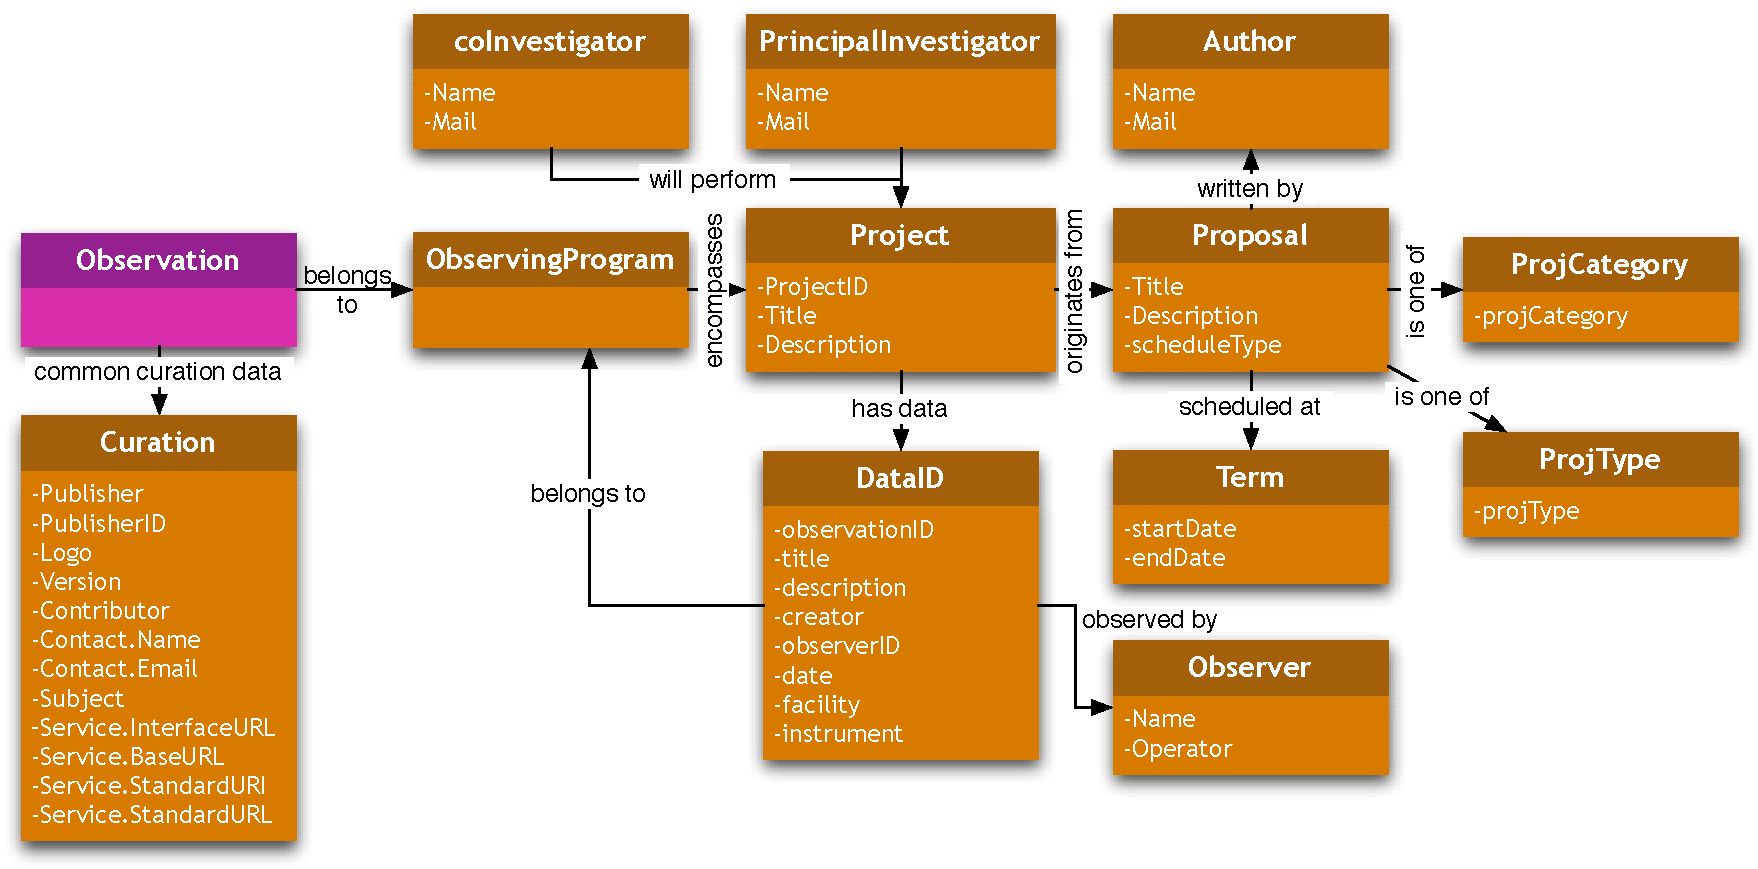
\includegraphics[width=\columnwidth]
				{fig/CurationClass.pdf}
			\end{center}
			\caption[Curation data model]{Curation data model.}
			\label{figCurationDataModel}
		\end{figure}
		
		\begin{description}
			\item[Observation]  The Observation class was
			discussed earlier. All observations are related to a single
			Curation class.

			\item[Curation]  This is the main class that will group
			all curation related metadata with relationships to
			complementary classes such as DataID and the rest.
			It is the same for all data contained in the VO resource
			(archive) being described.

			\item[DataID]  There is an instance of this class for
			each different piece of data stored, or at least for each
			different way to store data. The Spectral Data Model
			advocates for this separation.

			\item[ObservingProgram]  Instances of this class keep
			common information about different observations, describing
			its scientific or technical goals. They also specify which
			is the project and/or proposal to which this observing
			program belongs. This class allows for easy querying by
			project or by common goals, such as maser surveys.

			While there is debate about whether this class belongs to
			the Curation or to the Provenance Data Model, we believe it
			belongs to the Curation Data Model, as it is an
			organisational unit, and in our view it has nothing to do
			with how the data were taken.

			\item[Project]  This class is the main class from an
			organizational point of view. All observations belong to a
			single project through a single proposal. A
			Project instance is related to a collection of
			Proposal instances.

			\item[Proposal]  As stated in the Project
			class, a Project can be divided in a series of
			Proposals. A Proposal instance can be
			related to one or more observations. No observation can be
			related to more than one Proposal instance.

			\item[Author]  An Author instance contains
			information about Proposal authors.

			\item[Observer]  Observer instances represent
			the observer/s assigned to a Proposal. It also
			contains a relationship with a Contact acting as
			the operator for the instrument.

			\item[ProjCategory]  This instance specifies the
			scientific category of the project, from a controlled
			vocabulary; possible values, as specified by the Resource
			Data Model, are: \texttt{instrumental}, \texttt{galactic},
			\texttt{ter\-res\-tri\-al}, \texttt{so\-lar\-Sys\-tem},
			\texttt{ex\-tra\-ga\-lac\-tic}, \texttt{stellar}…

			\item[ProjType] This instance specifies the type of
			observation performed for a particular proposal.
			Possible values are specified by the Resource Data
			Model, and form a controlled vocabulary that we have
			derived from Lamb's, ATNF and NRAO
			proposals~\cite{2006astro.ph..1354, LamPow0310IVOA,
			PreCla0412Device}:
			\texttt{as\-trom\-e\-try},
			\texttt{band\-width\-Syn\-the\-sis},
			\texttt{cir\-cu\-lar\-Po\-lar\-i\-za\-tion},
			\texttt{con\-tin\-u\-um}, \texttt{en\-gi\-neer\-ing},
			\texttt{fill\-er\-Time},
			\texttt{high\-Time\-Res\-o\-lu\-tion},
			\texttt{im\-ag\-ing}, \texttt{in\-stru\-men\-tal},
			\texttt{lin\-e\-ar\-Po\-lar\-i\-za\-tion},
			\texttt{map\-ping}, \texttt{mon\-i\-to\-ring},
			\texttt{mo\-sa\-ic}, \texttt{mul\-ti\-beam},
			\texttt{point\-Source}, \texttt{phased\-Ar\-ray},
			\texttt{po\-lar\-im\-e\-try}, \texttt{snap\-shot},
			\texttt{so\-lar}, \texttt{spec\-tros\-copy},
			\texttt{sur\-vey}, \texttt{time\-Bin\-ning}.
			
			\item[Term] Specifies start and end dates (ISO dates,
			with time stamp) for the proposal \emph{observing term}
			or \emph{scheduling block}.
		\end{description}
		
		
		\invisiblenote{
		Describe the linking of the ObsData identifier with
		Curation; Curation should be linked from ObsData, as there
		will be a many to one relationship typically for most
		observations, but if several services are built with
		different characteristics (for instance, a most isolated
		galaxies catalogue from a more general galaxy catalogue).}
		
		\invisiblenote{
		\newcommand{\ivoacpigurl}[0]
		{http://www.ivoa.net/cgi-bin/twiki/bin/view/IVOA/IvoaCP}
		Integrate the existence of the IVOA Data Curation and
		Preservation interest group\urlnote{\ivoacpigurl}.}
		
	% section curation (end)
	
	\section{Policy} % (fold)
	\label{sec:policy}
		\attributedquote{
			\dictionarydef
				{policy}
				{noun}
				{
					\begin{itemize}
						\item a course or principle of action
						adopted or proposed by a government, party,
						business, or individual.
						
						\item \textsf{archaic} prudent or expedient
						conduct or action.
					\end{itemize}
				}
		}
		{The New  Oxford American Dictionary, \emph{2nd Edition}}
		
		\noindent
		The general definition above translates into the VO as
		\emph{data access policy}, and could be defined as
		the expedient action of granting or denying access to
		data following some principles proposed by data
		providers. Those principles take into account who is
		responsible for the data generation, for the data curation,
		and their relationship to the user trying to access the
		data.
		
		Moreover, those principles (policies) can change from
		institution to institution, and also for different datasets
		curated by those institutions. Hence, we need to generalise
		a way to specify those different policies, both regarding
		the different users' relationships with the datasets, and
		the different ways to implement policies, from
		\emph{everything is accessible}, to \emph{PI's eyes only}.
		
		\invisiblenote
		{\textbf{Rewrite this paragraph coming from the DEA
			Details chapter and Policy appendix to accommodate
			to the chapter style.}}
			
		The role of the Policy data model is to allow for very
		different policies to be applied to the data. In the case
		of a VO archive where the data are not immediately
		available (they have to be manually incorporated to the
		archive), Policy can become simpler, as in \emph{everything
		in the archive is available for everyone}.
		Figure~\ref{figPolicyDataModel} shows the different classes
		needed to characterise the archive policy.
			
		\begin{figure}[tbp]
			\begin{center}
				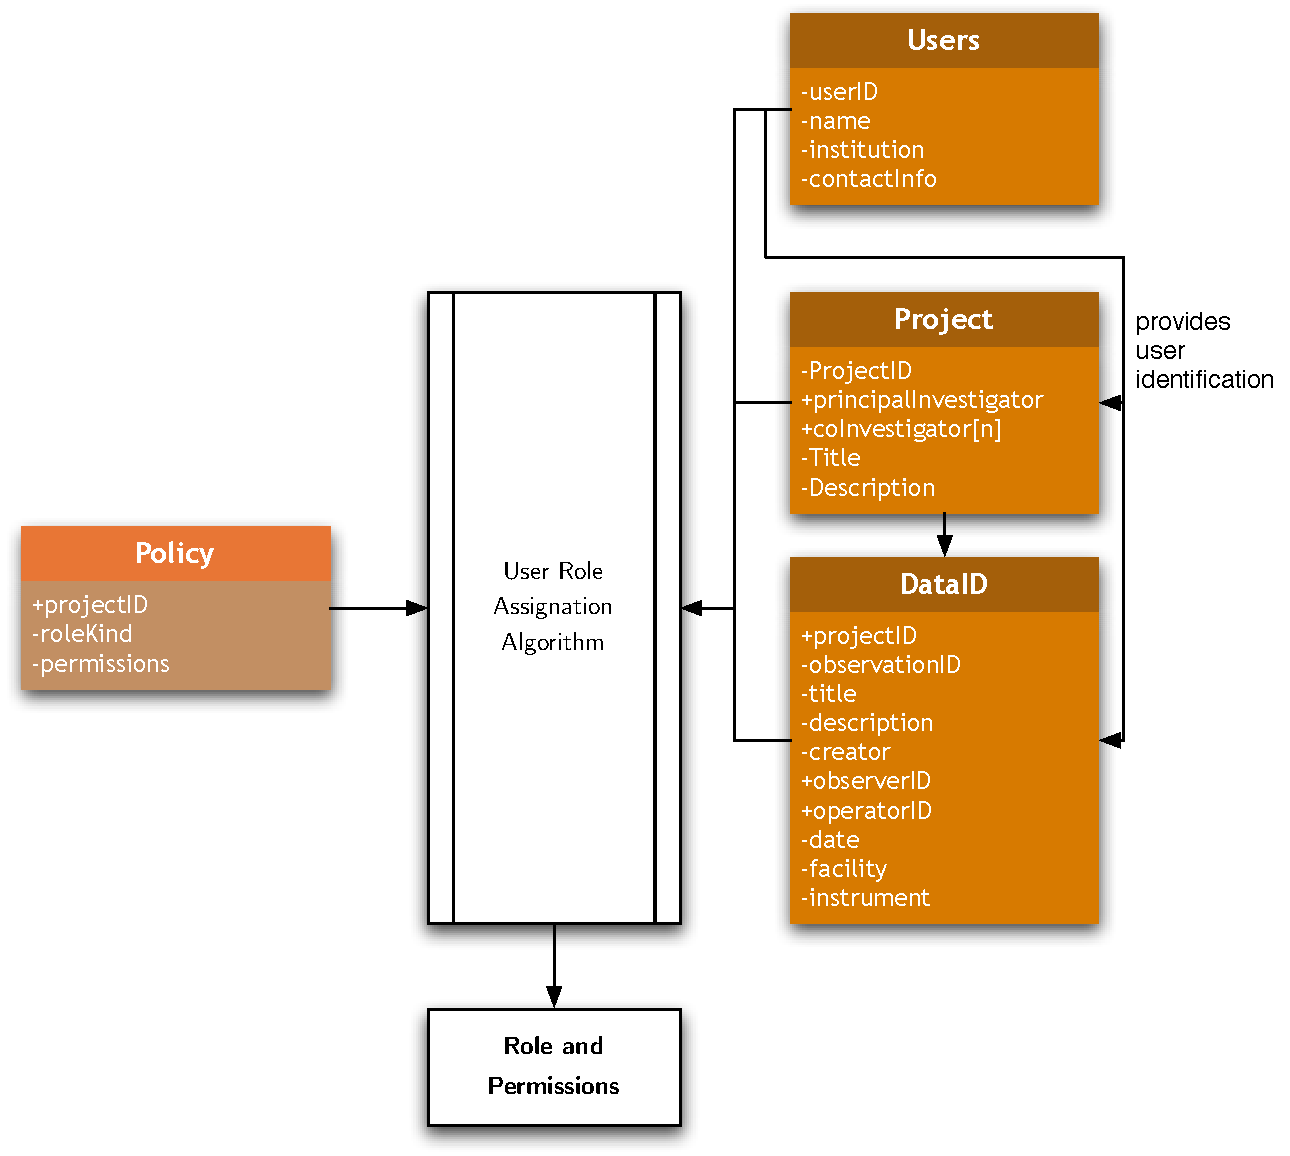
\includegraphics[width=\columnwidth]
				{fig/Policy-DM}
			\end{center}
			\caption[Policy data model]
				{Policy data model, with role and permissions.}
			\label{figPolicyDataModel}
		\end{figure}
		
		Policy instances attached to raw data shall need to
		identify the different roles of agents ---not just people,
		but software packages too--- accessing the archive, and give
		them appropriate access rights to pieces of data.
		
		 In the case of the Robledo Archive, the policy to be
		implemented should be the standard NRAO policy: 18 months
		since the end of the observations. Such a simple policy is
		better accomplished by not entering data into the archive
		until the proprietary period has expired.
		
		 A more flexible solution would make use of an array of
		permissions by role, where roles are derived from the
		relationship between the principal investigator and/or the
		observer, and observatory staff.
		
		 Such roles would be chosen from a controlled vocabulary
		(\texttt{prin\-ci\-pal\-In\-ves\-ti\-ga\-tor},
		\texttt{observer}, \texttt{co\-Inves\-tiga\-tor},
		\texttt{observatory\-Staff}, \texttt{none}); those roles
		are derived from user/project relationships, so that people
		not belonging to the observatory, and which have nothing to
		do with the project, would default to \texttt{none}.
		
		 Each project in the archive should have, at least, an
		explicit policy of what is allowed for some with none
		relationship with the Principal Investigator, and people
		with \texttt{prin\-ci\-pal\-In\-ves\-ti\-ga\-tor} roles
		have all access rights to the archive; people with roles
		other than \texttt{prin\-ci\-pal\-In\-ves\-ti\-ga\-tor}
		would fallback to the \texttt{none} role, if their role’s
		permissions are not explicitly declared.
		
		We will use Policy, Users and ObsData metadata in order to
		select the corresponding role for the agent just logged in.
		Figure~\ref{figPolicyRoles} shows the flow diagram for the
		role selection.
		
 		Policy metadata and attributes are specified in Table
		\ref{tabPolicyMetadata}, but also we will specify a subset
		of Curation attributes needed for successful Policy
		attribution.
		
		 We are also considering of establishing with the Policy
		data model data-oriented policies, instead of
		user-oriented. Data-oriented policies allow each
		datum ---possibly by means of the DataID or Project
		classes---
		to be searched and found, but no additional information, or
		only partial information —possibly having to do with the
		owner of the datum— can be retrieved, depending on the data
		policy in place. This needs at least an additional
		attribute in the DataID class.
		
		\begin{figure}[tbp]
		\begin{center}
		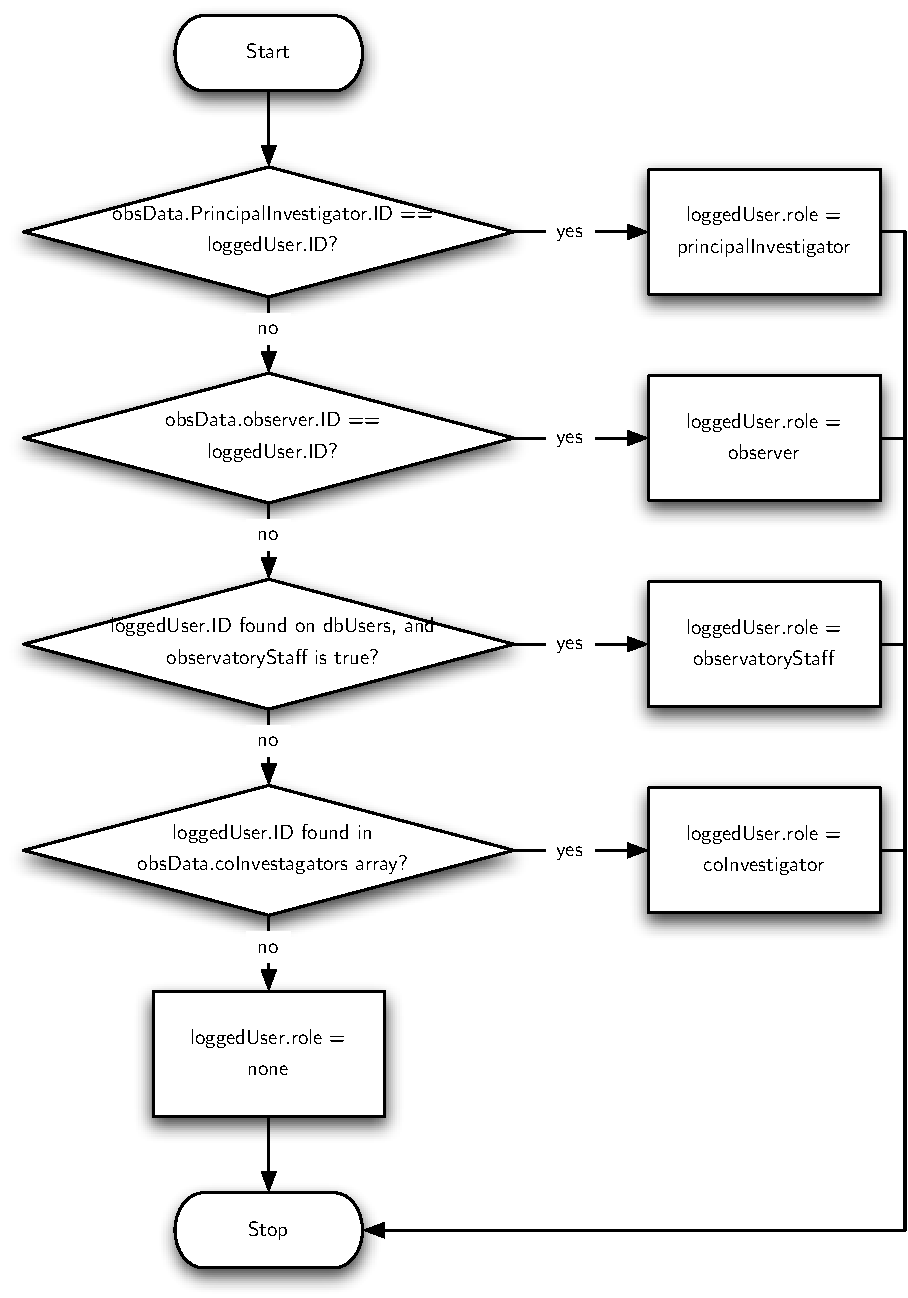
\includegraphics[width=\columnwidth]
			{fig/Policy-RoleDeterminationAlgorithm.pdf}
		\end{center}
		\caption[Role determination algorithm]
			{Flow diagram for the role determination algorithm.}
		\label{figPolicyRoles}
		\end{figure}
			
		This could be easily changed into a role-enabling algorithm
		that enables different roles for the same user, and
		displays all the different roles the user can access. If
		this is not needed, we will stick to the proposed
		algorithm.
		
		
		\begin{table}
		\begin{minipage}{\linewidth}
		\caption[Policy metadata]{Policy metadata.}
		\begin{smallertabular}{p{2.0 cm}p{1.25cm}p{3.6cm}p{4.4cm}}
				& \textbf{FITS} & & \\ \textbf{Attribute} & \textbf{Keyword} &
		        \textbf{UCD} & \textbf{Description}\\ \midrule projectID &
		        \texttt{PROJID} & \texttt{meta.curation.project;
		        meta.id}\footnote{There is no \texttt{meta.curation.project}
		        UCD, but we propose the inclusion of one.} & Project
		        identifier.\\ \addlinespace roleKind & \texttt{assign} &
		        \texttt{meta.policy.role; meta.code; meta.id}\footnote{There
		        are no \texttt{meta.policy.*} UCDs, but we propose, at least,
		        the inclusion of the \texttt{meta.policy} atom.} & Role kind
		        for which permissions will be provided.\\ \addlinespace permissions &
		        \texttt{assign} & \texttt{meta.policy.permissions;
		        meta.code}$^a$ & Permissions provided for roleKind users of
		        this project. The particular permissions to be provided are to
		        be discussed by IVOA.\\ \addlinespace
		\end{smallertabular}
		\label{tabPolicyMetadata}
		\end{minipage}
		\end{table}
		
		\begin{table}
		\begin{minipage}{\linewidth}
		\caption[Policy related Users metadata]{Policy related Users metadata.}
		\begin{smallertabular}{p{2.15 cm}p{1.5cm}p{2.35cm}p{5.25cm}}
				& \textbf{FITS} & & \\ \textbf{Attribute} & \textbf{Keyword} &
		        \textbf{UCD} & \textbf{Description}\\ \midrule
				
				userID & \texttt{COMMENT} & \texttt{meta.id} & User identifier
		        for all user related operations in the archive. \\ \addlinespace name
		        & \texttt{COMMENT} & \texttt{meta.name} & Real name of the
		        user. Any known user of the archive has to be registered, or be
		        anonymous. \\ \addlinespace institution & \texttt{COMMENT} &
		        \texttt{meta.name} & Name of the institution to which the user
		        belongs. \\ \addlinespace contactInfo & \texttt{COMMENT} &
		        \texttt{meta.note} & Contact info (probably e-mail) for this
		        user. \\ \addlinespace
		\end{smallertabular}
		\label{tabPolicyUsersMetadata}
		\end{minipage}
		\end{table}
		
		\begin{table}
		\begin{minipage}{\linewidth}
		\caption[Policy related Project metadata]
			{Policy related Project metadata.}
		\begin{smallertabular}{p{2.65 cm}p{1.5cm}p{3.3cm}p{3.80cm}}
				& \textbf{FITS} & & \\ \textbf{Attribute} & \textbf{Keyword} &
		        \textbf{UCD} & \textbf{Description}\\ \midrule projectID &
		        \texttt{PROJID} & \texttt{meta.curation.project;
		        meta.id}\footnote{There is no \texttt{meta.curation.project}
		        UCD, but we propose the inclusion of one.} & Project
		        identifier.\\ \addlinespace principalInvestigator & \texttt{COMMENT} &
		        \texttt{meta.id} & User identifier for the
		        principalInvestigator of the project. \\ \addlinespace
		        coInvestigator[n] & \texttt{COMMENT} & \texttt{meta.id} & User
		        identifier for the n\thsup\ co-investigator.\\ \addlinespace
		        title & \texttt{COMMENT} & \texttt{meta.curation.project;
		        meta.title}$^a$ & Project title.\\ \addlinespace description &
		        \texttt{COMMENT} & \texttt{meta.curation.project;
		        meta.note}$^a$ & Project description.\\ \addlinespace
		\end{smallertabular}
		\label{tabPolicyProjectMetadata}
		\end{minipage}
		\end{table}
		
		\begin{table}
		\begin{minipage}{\linewidth}
		\caption[Policy related DataID metadata]
			{Policy related DataID metadata.}
		\begin{smallertabular}{p{2.65 cm}p{1.5cm}p{3.3cm}p{3.80cm}}
				& \textbf{FITS} & & \\ \textbf{Attribute} & \textbf{Keyword} &
		        \textbf{UCD} & \textbf{Description}\\ \midrule projectID &
		        \texttt{PROJID} & \texttt{meta.curation.project;
		        meta.id}\footnote{There is no \texttt{meta.curation.project}
		        UCD, but we propose the inclusion of one.} & Project
		        identifier.\\ \addlinespace observationID & \texttt{OBSID} &
		        \texttt{obs; meta.dataset; meta.id} & User identifier for the
		        principalInvestigator of the project. \\ \addlinespace
		        coInvestigator[n] & \texttt{COMMENT} & \texttt{obs; meta.id} &
		        User identifier for the n\thsup\ project co-investigator.\\
		        \addlinespace title & \texttt{COMMENT} &
		        \texttt{meta.curation.project; meta.title}$^a$ & Project
		        title.\\ \addlinespace description & \texttt{COMMENT} &
		        \texttt{meta.curation.project; meta.note}$^a$ & Project
		        description.\\ \addlinespace creator & \texttt{AUTHOR} &
		        \texttt{meta.curation; meta.id} & User identifier for the
		        creator of the data entry.\\ \addlinespace observerID &
		        \texttt{OBSERVER} & \texttt{obs.observer; meta.id} & User
		        identifier for the person performing the observation producing
		        this data entry.\\ \addlinespace operatorID & \texttt{OBSERVER} &
		        \texttt{obs.operator; meta.id}\footnote{We propose the
		        inclusion of either \texttt{obs.operator} or
		        \texttt{instr.operator} as new UCDs to characterise
		        operator-related data. However, \texttt{obs.observer} can be
		        used when providing both observer and operator at the same
		        time.} & User identifier for the person performing operator
		        duties while performing the observation.\\ \addlinespace date &
		        \texttt{DATE-OBS} & \texttt{time.obs.start} & Date of
		        observation.\\ \addlinespace facility & \texttt{TELESCOP} &
		        \texttt{instr.obsty} & Facility (observatory) where the
		        telescope/instrument resides in.\\ \addlinespace instrument &
		        \texttt{INSTRUME} & \texttt{instr.tel} & Instrument performing
		        the observation\footnote{We have to study whether this should
		        contain an instrument-backend pair, or have different
		        attributes for both.}.\\ \addlinespace
		\end{smallertabular}
		\label{tabPolicyDataIDMetadata}
		\end{minipage}
		\end{table}
		

	% section policy (end)
	
	\section{Packaging} % (fold)
	\label{sec:packaging_the_vopack}
		
		\attributedquote{
			\dictionarydef
				{packaging}
				{noun}
				{
					\begin{itemize}
						\item materials used to wrap or protect
						goods.
						
						\item the business or process of packing
						goods.
						
						\item the presentation of a person,
						product, or action in a particular way.
					\end{itemize}
				}
		}
		{The New  Oxford American Dictionary, \emph{2nd Edition}}
		
		Digital data are usually thought of as free of \emph{bit
		rot}: digital copies are always bit perfect, but that is
		so because a lot of care is put into providing enough
		redundancy on the storage and interchange processes, so that
		possible bit flips can be detected and corrected.
		
		But changes in content can also be produced on
		intermediate states for a dataset: imagine reduced data
		products for which the calibration has been changed,
		producing at the same time a change in characterisation.
		The new data product being provided might link to an
		updated data product, but its characterisation can be
		the old one. Thus, we need a way to provide a permanent
		set of data products, which can be easily combined without
		further service queries by means of attached
		characterisation instances.
		
		\invisiblenote{
			\textbf{Rewrite this text coming from the DEA, both
			the Details chapter and VOPack appendix.}}
			
			The Packaging class is used to specify how data from
			different sources will be presented together. For
			instance, if we wanted to retrieve data belonging to
			our already mentioned maser survey, a VO system could
			reply with a Multi-Beam FITS file containing all the
			scans and sub-scans that conform the On-Off patterns for
			a single issued observation, or with a \texttt{.zip}
			file with all the FITS files belonging to the survey,
			or with just a single On-Off pair, et cetera.
			
			 An instance of the Packaging class would describe the
			contents of the data retrieved, in terms of project
			organisation, and of the particular files being
			actually delivered.
			
			 Unfortunately, there is no Packaging class defined at
			the VO level, so we have to resort to other packaging
			description mechanisms available in other archiving
			tools.
			
			First, we have to state the requirements for this class:
			
			\begin{itemize}
				\item The Packaging class will describe the type of
				compression or grouping, if any, applied to the
				result of a query. So, possible results should form
				a controlled vocabulary, such as \texttt{FITS},
				\texttt{VOTable}, \texttt{zip}, \texttt{tar},
				\texttt{gz}, \texttt{bz}, \texttt{bz2},
				\texttt{tgz}, \texttt{tbz}, \texttt{tbz2},
				corresponding to: raw files ---a FITS file or a
				VOTable---, a zip file, a tar file, a raw file
				compressed by gzip, bzip, bzip2, and a gzipped,
				bzipped or bzipped2 tar file.
				
				 \item We believe a standard VO packaging scheme is
				needed in order to facilitate distribution. We
				propose one such scheme, that we call VOPack
				---Virtual Observatory Package; \texttt{.vopack}
				file extension---. We will define the VOPack as a
				“tarred and gzipped” folder (\texttt{.tgz} file)
				with an XML content descriptor, which acts as
				VO-aware manifest of contained assets.
			\end{itemize}
			
			The VOPack is a way of distributing VO-compliant
			content, in a way that makes it easy to reuse and point
			to existing content, either remote or locally.
			
			A VOPack consists of a compressed file that contains at
			least a \texttt{voPack.xml} file —following the VOPack
			XML Schema— that describes all the additional content
			of the compressed VOPack, and their relationships
			between them. Figure~\ref{figVOPackStructure} shows the
			structure diagram of a VOPack.
			
			\begin{figure}[tbp]
			\begin{center}
				%\includegraphics[scale=1]{VOPackStructure.pdf}
				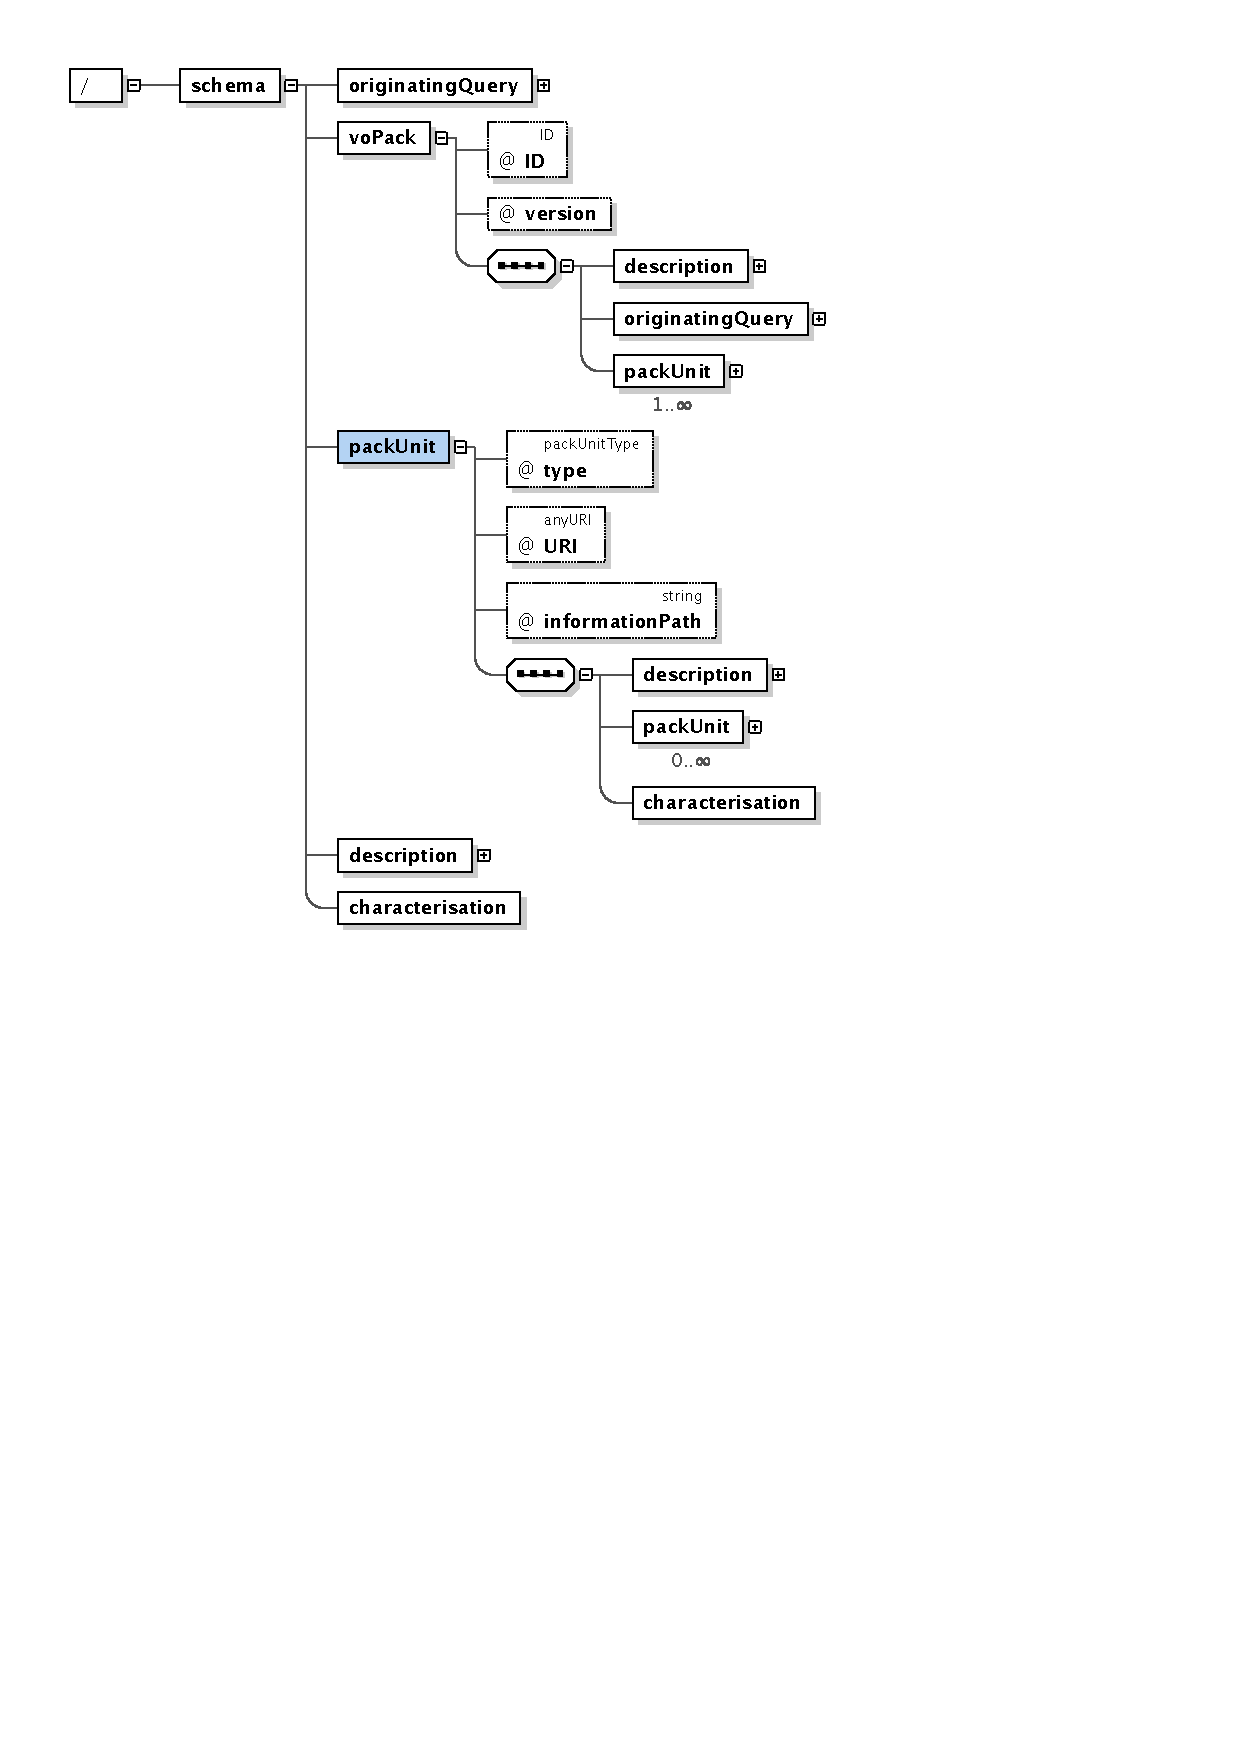
\includegraphics[scale=0.5]
				{fig/vopack-structure.pdf}
			\end{center}
			\caption[VOPack structure]
			{
				VOPack structure. Diagram generated by
				\textbf{Oxygen} from the XML schema.
			}
			\label{figVOPackStructure}
			\end{figure}
			
			In that diagram, the \texttt{voPack} element is the
			root for the XML document. It includes a description,
			the originating query, and one or more
			\texttt{packUnits}, which actually point to the
			information being retrieved. The
			\texttt{o\-rig\-i\-na\-ting\-Que\-ry}
			element contains the string
			with the URI that allows the retrieval of the voPack.
			Additional \texttt{characterisation} elements,
			following the Characterisation schema, can be used to
			further specify properties on the data being delivered
			with the VOPack.
			
			The \texttt{packUnit} corresponds to a single piece of
			data, or to another \texttt{packUnit}s, in case of more
			structured data. The depth of inclusion is arbitrary.
			
			\texttt{packUnit}s have a \texttt{type} attribute that
			can be one of:\texttt{votable}, \texttt{fits},
			\texttt{vopack}, \texttt{compressedFolder},
			\texttt{folder}, \texttt{otherXML},
			\texttt{otherNonXML}. Table~\ref{packUnitType}
			specifies the meaning of this attribute.
			
			\begin{table}
				\caption[Valid \texttt{packUnit} attribute values]{
					Meaning of the different valid values for
					attributes of the
					\texttt{packUnit} data type.
				}
				\begin{smalltabular}{rp{9.75cm}}
					\textbf{packUnit} &- \textbf{Description}
					\\\midrule
					
					 \texttt{votable} & The packed unit is a
					VOTable. \\\addlinespace
					
					 \texttt{fits} & The packed unit is a FITS
					file. \\\addlinespace
					
					 \texttt{vopack} & The packed unit is itself a
					VO pack. The characterisation of the
					referencing VO pack encompasses all packed
					units, while each particular one will have its
					own, \emph{narrower} characterisation.
					\\\addlinespace
					
					 \texttt{compressedFolder} & The referenced
					packed unit is a compressed directory.
					\\\addlinespace
					
					 \texttt{folder} & The referenced packed unit
					is a directory in the same file-system as the
					referencing VOPack. \\\addlinespace
					
					 \texttt{otherXML} & An XML representation,
					other than a VOTable, is used. \\\addlinespace
					
					 \texttt{otherNonXML} & A non-XML
					representation, also different from a FITS
					file, is used. This kind of representation
					should be avoided, but would be useful for
					packing instrument specific raw data formats,
					which are correctly characterised.
					\\\addlinespace \end{smalltabular}
					\label{packUnitType}
			\end{table}
			
			For the \texttt{vopack}, \texttt{folder} and
			\texttt{compressedFolder} values, a new
			\texttt{vopack.xml} file has to be provided for their
			description. This allows for meta-packaging of
			ready-made VOPacks.
			
			 For the first three types, the
			\texttt{informationPath} attribute gives an XPath to
			the actual data being pointed, just in case the
			\texttt{packUnit} contains several tables, and not all
			of them are to be considered. In the case of FITS
			files, the informationPath looks XPath-like, but points
			to the HDU or Image holding the data.
			
			 Figure~\ref{figVOPackXSDfile} shows the complete
			listing for the VOPack XML Schema.
			
			\begin{figure}[tbp]
			\begin{center}
				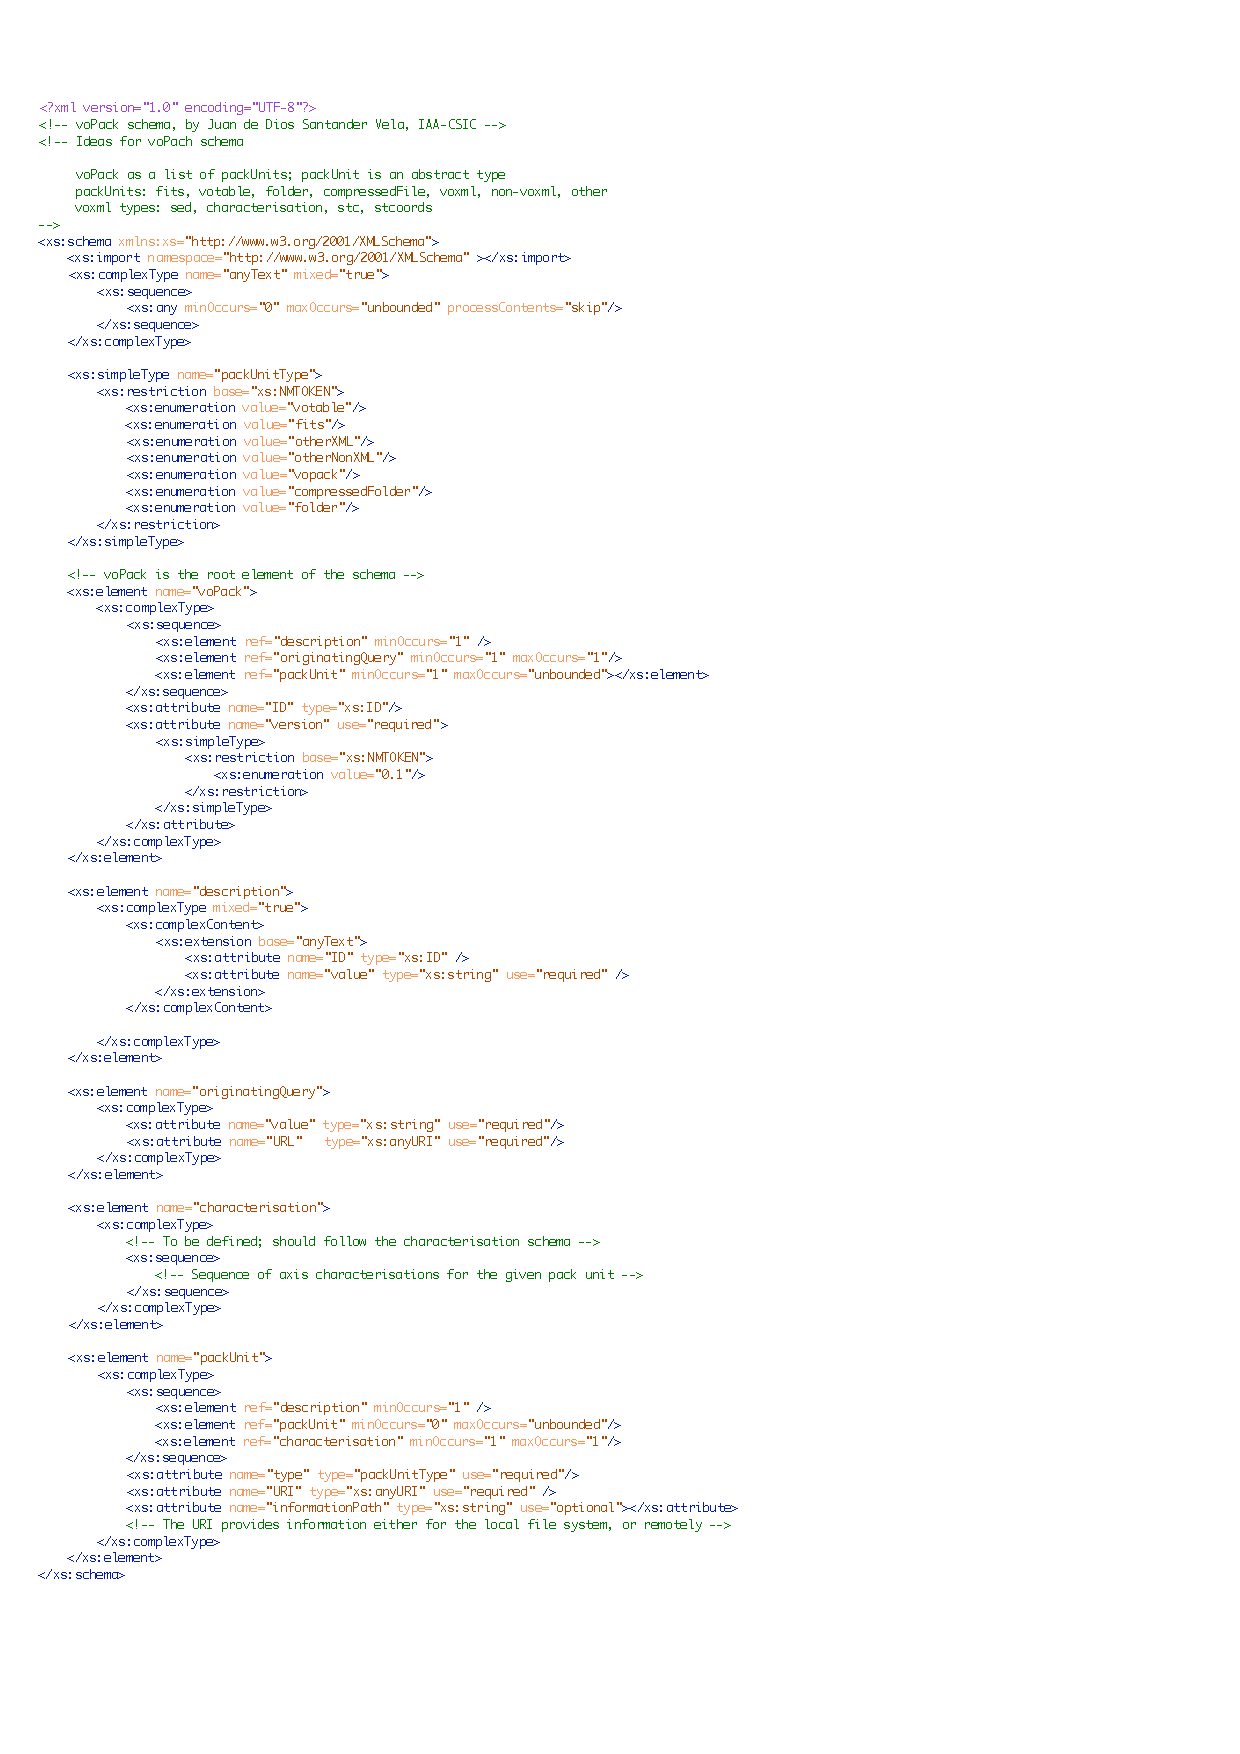
\includegraphics[totalheight=1\textheight]
				{fig/vopack-schemaListing.pdf}
			\end{center}
			\caption[VOPack schema listing]
			{VOPack XSD schema listing.}
			\label{figVOPackXSDfile}
			\end{figure}
			
			The VOPack XML Schema has been inspired by the concepts
			of Digital Items, Digital Item Containers, and Digital
			Item Components from MPEG-21~\cite{Bormans:fk}.
		
		
	% section packaging_the_vopack (end)
	
	\section{Conclusions} % (fold)
	\label{sec:radams_curation_etc_conclusions}
		
		In this chapter we have dealt with generic astronomical
		concepts, non-specific of radio astronomy, but which 
		were needed both for implementing the suggested ObsDM
		entities, but also for being able to successfully use IVOA
		data models as blueprints for archive development, as it
		will be shown when applying the data model to the archives
		of DSS-63 and IRAM~30m in
		chapter~\ref{cha:radams_based_archives}.
		
	% section radams_curation_etc_conclusions (end)
	
% chapter radams_curation_packaging_and_policy (end)
	%2345678901234567890123456789012345678901234567890123456789012345678901
\chapter{Data Provenance} % (fold)
\label{cha:data_provenance_in_the_vo}

	%\section{Introduction} % (fold)
	%\label{sec:vo_provenance_introduction}
	%
	%% section vo_provenance_introduction (end)

	\attributedquote{
		\dictionarydef
			{provenance}
			{noun}
			{
				\begin{itemize}
					\item the place of origin or earliest known
					history of something.
					
					\item the beginning of something's existence;
					something's origin.
					
					\item a record of ownership of a work of art
					or an antique, used as a guide to authenticity
					or quality.
				\end{itemize}
			}
	}
	{The New  Oxford American Dictionary, \emph{2nd Edition}}
	
	\noindent
	The dictionary definition above points to the main three
	elements to which data provenance in e-Science has to deal
	with: Attribution, i.e. proper acknowledgement of authorship
	and or origin; Data Quality; and Replication of results, i.e.,
	the chain of processes needed to derive a result, beginning
	with data sources.
	
	 In the VO context, we can synthesise a definition by stating
	that Provenance (data provenance) is the record of the earliest
	known history of an astronomical data set, to be used as a
	guide to data quality and of data ownership.
	
	 Astronomical datasets use the data coming from different
	photons\footnote{Their arrival rate, their energy distribution,
	the positions from the sky, the difference with properties of
	photons not coming from the observed region; in addition, the
	response to photons, and to their absence, has also to be
	determined.} to derive physical properties from the observed
	objects. Therefore, data provenance ---also known as
	\emph{lineage} information--- in astrophysics is, in fact, the
	answer to the question \emph{What was done to this collection
	of photons, and which systems did it?}
	
	\section{Provenance in e-Science} % (fold)
	\label{sec:provenance_in_escience}
	
		As we have already established, data Provenance in the
		Virtual Observatory is just a specific form of the
		problem of data Provenance in e-Science, so in order
		to establish how to model astronomical data provenance,
		we will study first the different data provenance
		recording and determination techniques already
		available.
		
		\begin{figure}[tbp]
			\centering
				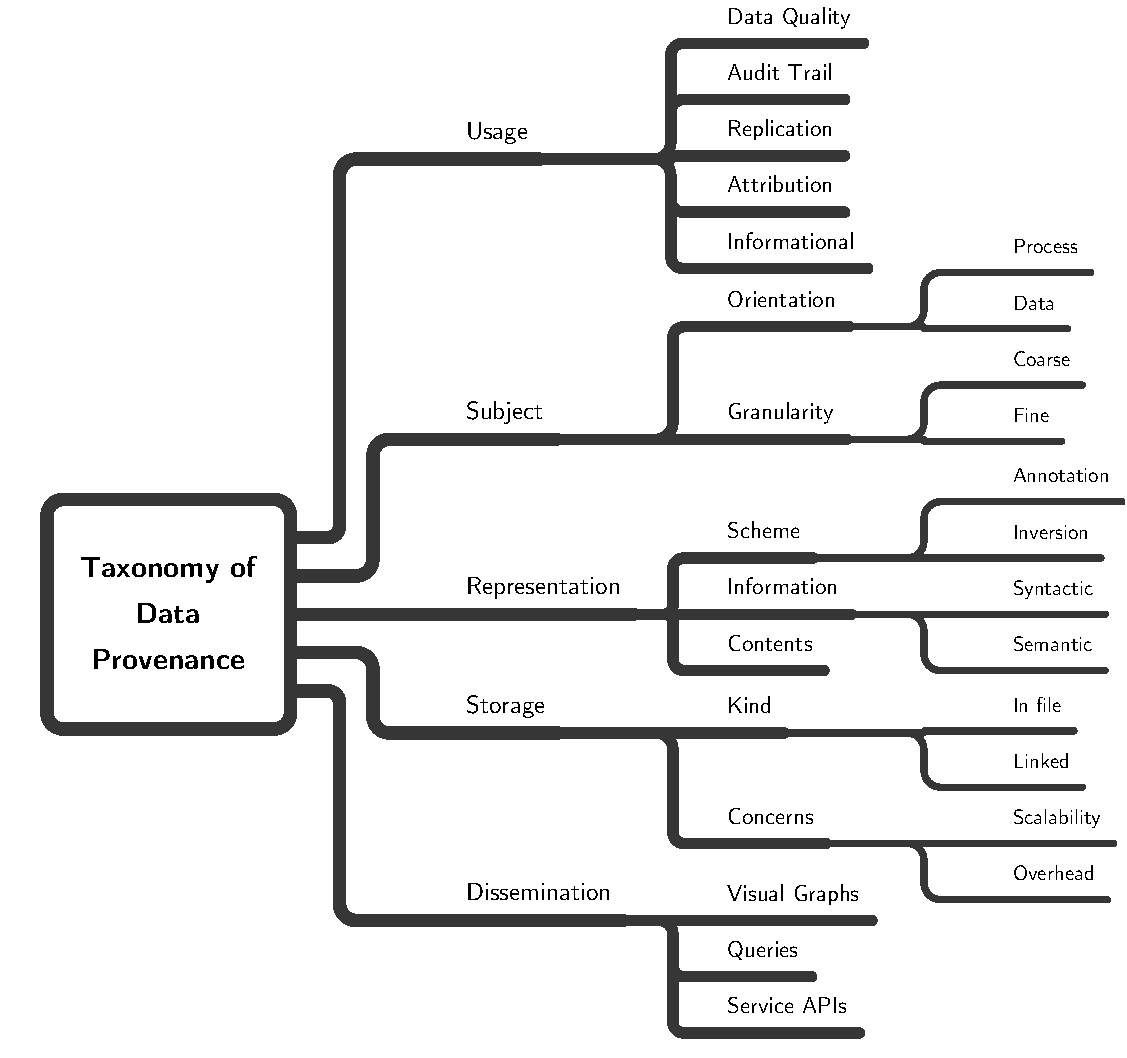
\includegraphics[width=\columnwidth]
				{fig/DataProvenanceTaxonomy.pdf}
			\caption[
				Taxonomy of data provenance techniques in
				e-Science
			]
			{
				Taxonomy of data provenance techniques in
				e-Science. Those techniques can be classified
				depending on the use of the provenance data
				collected, on the actual subject of data
				provenance, or the way data provenance is
				represented, stored, or disseminated. Based on
				\emph{A Survey of Data Provenance in
				e-Science}~\cite{SimPlaGan0503A-Survey}.
			}
			\label{fig:fig_DataProvenanceTaxonomy}
		\end{figure}
		
		In the paper \emph{A Survey of Data Provenance in
		e-Science}~\cite{SimPlaGan0503A-Survey} by Simmhan et al.
		many different data provenance collection techniques are
		studied, and a taxonomy of them is created ---see
		figure~\ref{fig:fig_DataProvenanceTaxonomy}---, depending
		on:
		
		\begin{description}
			\item[Usage] Data provenance information can be used
			for estimating data quality and data reliability, or to
			provide an audit trail of the data transformations. It
			can also be used to replicate an experiment, to
			attribute the creation of a dataset to a set of
			original (in the sense of originating) data, and to the
			set of processes needed to derive the new dataset. Or
			it can be informational, without providing enough
			information to assess any of the above.
			
			\item[Subject] Data provenance can be focused on the
			data themselves, collecting lineage metadata from each
			data product, or on the processes on the data. And in
			any case the recorded provenance can be coarse grained
			(for instance, describing a whole set of data) or fine
			grained (describing each single datum and/or process;
			for instance, database tuples' attributes).
			
			\item[Representation] The way data provenance can be
			represented is also diverse, and some of them depend on
			the processing system being studied. The two main
			approaches in the literature are annotations and
			inversion. Annotations are \emph{a priori} provenance
			metadata: the transformed data are accompanied by
			provenance metadata which has been created prior to the
			transformation. On the other hand, inversion data
			provenance is created \emph{a posteriori} from the data
			products of a transformation which can be inverted,
			with provenance metadata being created from the
			documentation of the process and the differences
			between inputs and outputs. It is clear that inversion
			metadata are more compact, while annotations can
			include parameters of processes, their versions, and
			even references to publications.
			
			 As some of the lineage information implies
			relationships between datasets and processes, that
			information can be captured in data models about the
			processes, or using semantic web technologies, such as
			the RDF and OWL languages, in order to describe such
			relationships. In this way, the process semantics are
			documented. In any case, the process syntax is
			specified from the input data, the output data, and
			annotations, if present.
			
			\item[Storage] As provenance metadata can be generated,
			collected and/or transmitted at many different places,
			there must be a way to keep those metadata stored,
			while keeping the relationship with the data
			themselves. Depending on the grain of the metadata
			collection process, and on whether the lineage
			information is just updated or versioned, the amount of
			provenance metadata can grow several orders of
			magnitude above the original data. Both the overhead of
			provenance metadata (percentage of storage devoted to
			provenance versus data, and cost of metadata
			management), and the scalability of the system, that
			is, how to deal with the provenance metadata if the
			data rate increases an order of magnitude.
			
			\item[Dissemination] Finally, provenance metadata are
			gathered for applications to use them. Typical ways of
			disseminating lineage information are by means of
			derivation graphs~\todoinlinesuspended{\citeneeded},
			but in many cases where
			the provenance metadata are stored inline with the data
			the form is just a list of time-stamped annotations. If
			semantic web tools are used, workflows can determine
			the input provenance information and create the
			dissemination graph at runtime. In addition, specially
			in cases were lineage metadata are stored in databases
			or XML documents, provenance specific queries can be
			performed, and even provenance query APIs can be created
			so that different systems can access such information.
			
		\end{description}
	
		Another classification~\cite{Buneman:2001fc}
		of Provenance data can be performed regarding how it
		is collected or computed:
		
		\begin{description}
			\item[Why provenance] Refers to the reason why a datum
			is in a given dataset, i.e., the query that was
			performed, including data sources. For data coming from
			database queries, different fields can have different
			sources, but all fields, and many rows derived from the
			same query, will share that query. In a sense,
			\emph{Why} provenance is a proof that a datum belongs
			to a processed (queried) data set, as it corresponds to
			the minimum set of sources and sources' entries which,
			together with the query being performed, will provide
			that datum as an answer.
			
			\item[Where provenance] Refers to the actual
			progenitors of each particular datum, i.e., what
			particular database tuple, and field in the tuple,
			provided the datum we are analysing.
		\end{description}
		
		The difference between both kinds can be better illustrated
		using a database originated example.
		Let us imagine the SQL query:
		
		\begin{adjustwidth}{\parindent}{\parindent}
			\noindent\texttt{SELECT name, telephone\\
			FROM employee\\
			WHERE salary > (SELECT AVERAGE salary FROM employee)}
		\end{adjustwidth}
		
		 And let us say one of the tuples in the result is
		\texttt{("John Doe", 555123467)}. As all rows in
		\texttt{employee} where needed for the calculation of the
		salary average, a change in any row could make our target
		tuple disappear from the result list, so the \emph{Why}
		provenance is the query plus the \texttt{salary},
		\texttt{name} and \texttt{telephone} fields of all rows of
		the \texttt{employee} table. The \emph{Where} provenance,
		however, is only concerned with the actual progenitor of
		each of the tuple's datum, and the answer is the
		\texttt{name} and \texttt{employee} fields of the row
		containing John Doe's entry in the \texttt{employee} table.
		
		Finally, another difference can be established for
		data provenance collection systems, depending on the
		data collection strategy:
		
		\begin{description}
			\item[Eager collection] Lineage information is
			created/computed after each transformational or
			derivational step.
			
			\item[Lazy collection] Provenance information is
			calculated on demand, using specific knowledge of
			the transformations, and parameters saved.
		\end{description}
		
		We will end up our review
		of data provenance systems and classifications
		by showing table~\ref{provenanceSystems} of
		different data provenance management systems in different
		application areas, and see their characteristics.
		
		We can see that most
		of the systems assume a relational database
		infrastructure, and rely on annotations for carrying
		on provenance information. Only systems completely
		contained within a relational database systems use
		inverse queries or functions for their recovery of
		data provenance.
		
		\begin{sidewaystable}
		\begin{minipage}{\linewidth}
		\caption[Data provenance management systems' properties]
		{
			Properties of different data provenance management
			systems for different scientific domains, as compiled
			by~\cite{SimPlaGan0503A-Survey}.
		}
		\label{provenanceSystems}
		\begin{scriptsizetabular}
		{p{2.25cm} p{1.66cm} p{1.66cm} p{1.66cm} p{1.66cm} 
		 p{1.66cm} p{1.66cm} p{1.66cm} p{1.66cm} p{1.66cm}}
		
			& \textbf{LIP} & \textbf{Chimera} & \textbf{myGRID} &
			\textbf{CMCS} & \textbf{PASOA} & \textbf{ESSW} &
			\textbf{Tioga} & \textbf{Buneman} & \textbf{Trio} \\
			\midrule
			
			Domain\footnote{GIS: Geographical Information System}
			& GIS & Physics, Astronomy & Biology & Chemistry &
			Biology & Earth Sciences & Atmospheric Sciences &
			Generic & Generic \\ \addlinespace
			
			Processing\footnote{RDBMS: Relational Data Base
			Management System} & Commands & Services & Services &
			Services & Services & Scripts & RDBMS & RDBMS & RDBMS
			\\ \addlinespace
			
			Application\footnote{Kind of Provenance application:
			I: Informational; R: Regeneration; A: Audit; E: Error
			Tracking; U: Information Update; P: Planning} & IR &
			IRAP & IR & IU & IR & I & IE & IU & IU \\
			\addlinespace
			
			Orientation & Data & Process & Process & Data &
			Process & Data \& Process & Data & Data & Data \\
			\addlinespace
			
			Granularity & Spatial layers & Abstract datasets
			(files) & Abstract resources & Files & Workflow
			Parameters & Files & DB Attributes & DB Attributes \&
			Tuples & DB Tuples \\ \addlinespace
			
			Representation & Annotations & Annotations &
			Annotations & Annotations & Annotations & Annotations
			& Inverse functions & Inverse queries & Inverse
			queries \\ \addlinespace
			
			Semantics & No & No & Yes & Limited & No & Proposed &
			No & No & No \\ \addlinespace
			
			Storage\footnote{RDBMS: Relational Data Base
			Management System; N/A: Not available} & RDBMS & RDBMS
			& RDBMS & RDBMS & RDBMS + File System & RDBMS & RDBMS
			& N/A & RDBMS \\ \addlinespace
			
			Overhead & user commands; MD entry & user definition;
			automatic WF & service semantics; WF calls & service
			calls; working portal & manual & manual & manual
			registry of inverse functions & N/A & Automatic
			generation of inverse queries \\ \addlinespace
			
			Scalability & No & Yes & No & No & Proposed &
			Proposed & Yes & N/A & No \\ \addlinespace
			
			Dissemination\footnote{N/A: Not Available} & Queries
			& Queries & Semantic browser; Lineage graph & Queries;
			Browsing & Queries & Browsing & Queries; Graph & N/A &
			Queries
		\end{scriptsizetabular}
		\end{minipage}
		\end{sidewaystable}
		
		So, in order to establish a Data Provenance framework for
		the Virtual Observatory we will have to establish all of
		the items above: how to collect the information, which will
		be the intended use, and how is the information going to be
		represented, stored, and presented to intended users and
		systems; whether we need a \emph{Why} or \emph{Where}
		provenance system depending on typical VO use cases; and if
		such system must be \emph{Eager} or \emph{Lazy}, again
		depending on use cases.
		
	% section provenance_in_escience (end)

	\section{Provenance in astronomy and astrophysics} % (fold)
	\label{sec:provenance_in_astronomy_and_astrophysics}

		After the classification above, we will study the different
		data provenance techniques in use within the astronomy,
		together with their intended application.
		
		Typically, one of the uses of header cards in FITS files is
		storing \texttt{COMMENTS} and \texttt{HISTORY} cards.
		Figure~\ref{fig:fig_FITSHeadersProvenance} shows an example
		of a FITS file processed by the
		AIPS\urlnote{http://www.aips.nrao.edu/} interferometric
		data reduction software.
		
		\begin{figure}[tbp]
			\centering
				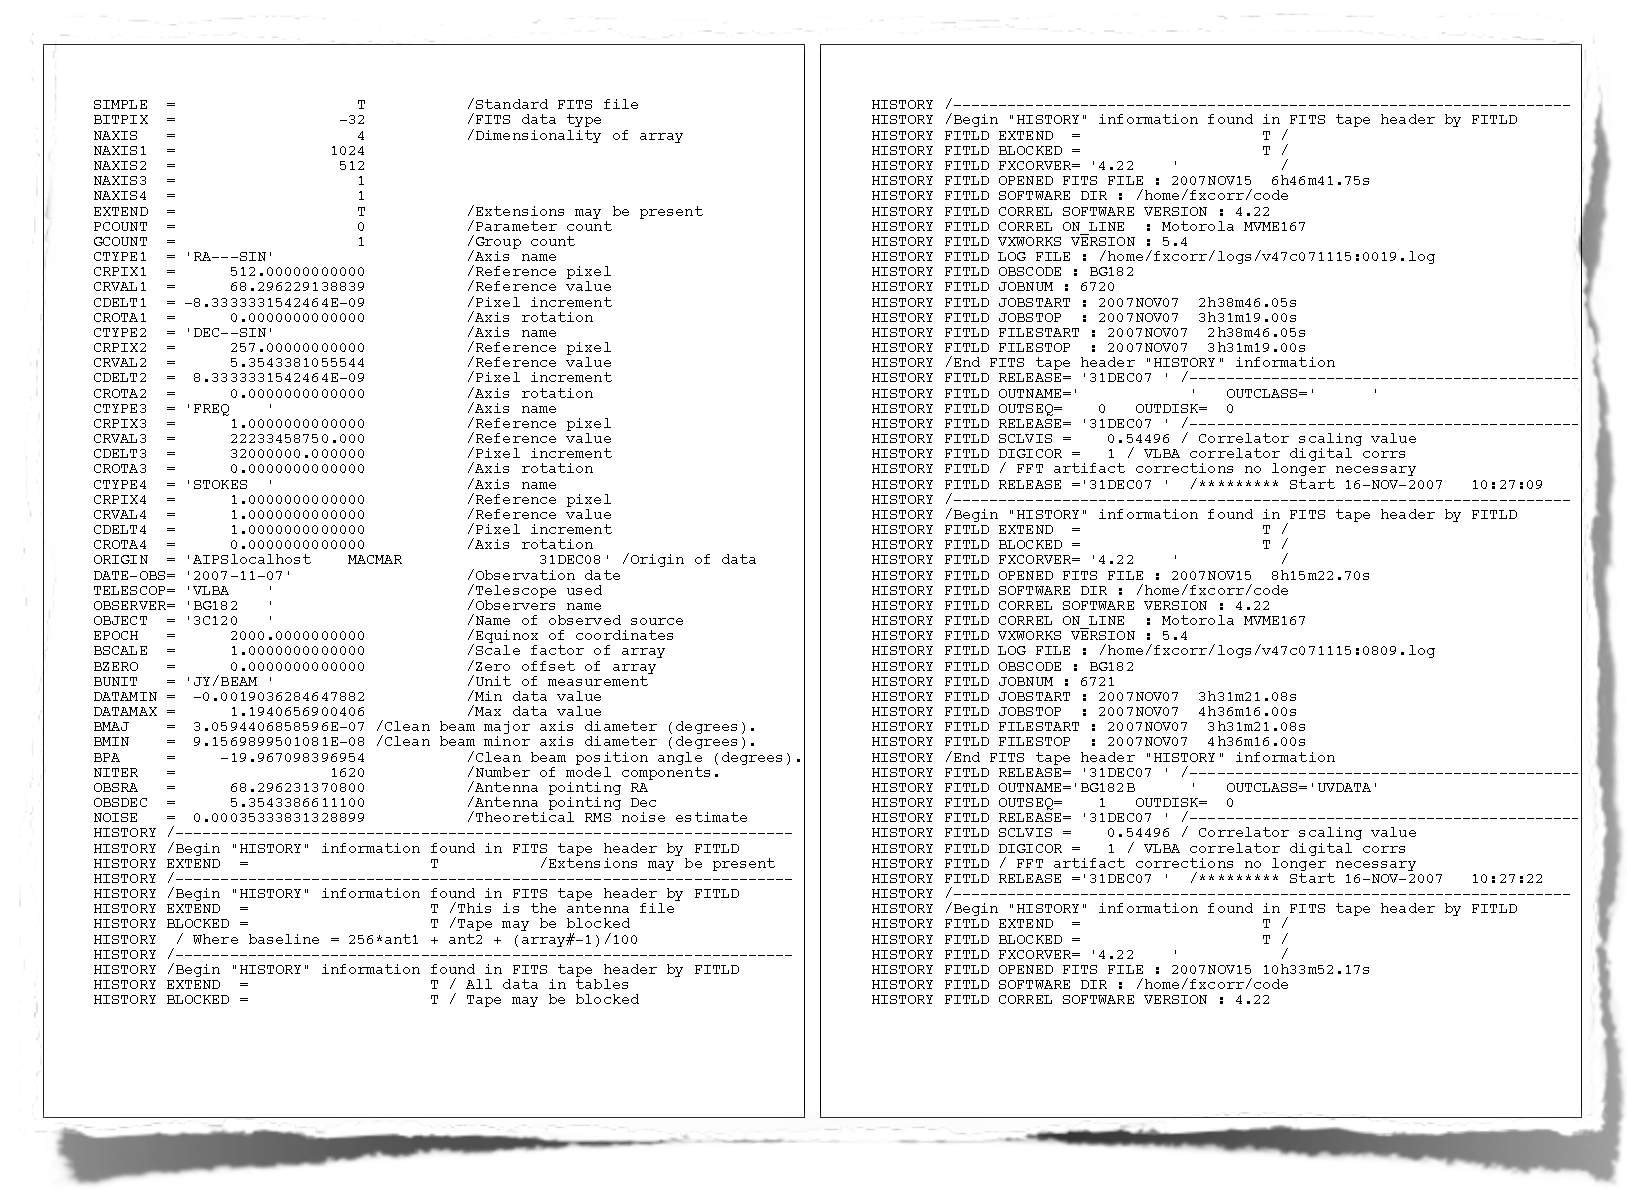
\includegraphics[width=\columnwidth]
				{fig/FITSHeadersProvenance.pdf}
			\caption[FITS headers showing AIPS History]{
				A pair of pages of FITS headers from a file which
				has been processed with the AIPS radio
				interferometry data reduction and imaging software.
				The first page starts with the headers establishing
				the axes for the observation (RA, Dec, Frequency
				and a fixed polarisation), and after that
				\texttt{HISTORY} tags start documenting the
				different calls to different AIPS tasks
				(\texttt{FITLD}, FITS LoaD, is the first one
				called by AIPS in order to create the AIPS data
				structures from the contents of the FITS file).
			}
			\label{fig:fig_FITSHeadersProvenance}
		\end{figure}
		
		In that figure we can see an example of how typical
		astrophysical tools have been dealing with data provenance.
		Each different application can make use of the FITS header
		cards, specifically of the \texttt{HISTORY} keyword, in
		order to provide feedback of the steps being performed on
		the data.
		
		 In this case, the data provenance being provided is of the
		\emph{Why} kind, albeit not complete. Apart from the text
		\emph{annotation} on the FITS headers, tables of task
		Parameters are stored within the FITS file itself, so this
		provenance information is collected \emph{eagerly}, and
		corresponds to \emph{Why} provenance. If all the operations
		where invertible, it would also provide an invertible
		\emph{Where} provenance, but some of the data is lost
		during each processing step.
		
		\newcommand{\difmapurl}[0]
		{ftp://ftp.astro.caltech.edu/pub/difmap/difmap.html}
		However, that is the case for a particular package. The
		FITS headers added by the difmap
		package\urlnote{\difmapurl}, for example, only indicate
		that difmap has touched the file somehow, without any
		details:
		
		\begin{adjustwidth}{\parindent}{\parindent}
			\noindent\texttt{HISTORY DIFMAP  Read into difmap
			on Sun Jul 10 17:00:50 1994\\
			HISTORY DIFMAP  Saved clean-map to fits file.}
		\end{adjustwidth}
		
		So, we can see that there is a provision in FITS files to
		allow for provenance information to be stored, but the
		convention for provenance coding depends entirely on
		the application. Conversely, it can be said that there is
		no convention in use to be adapted for the VO usage.
		
		In the VO framework, arbitrary \xmltags{RESOURCE} can be 
		included, which can be used to include and/or link, to
		arbitrary data, so we already have the support within
		the VOTable to add that information.
		
		In order to make Provenance usable by VO tools
		we need to provide a framework which:
		
		\begin{itemize}
			\item allows flexibility in the amount of
			metadata being provided;
			
			\item allows queries on metadata which are relevant
			in order to find datasets which have given common
			properties;
			
			\item integrate not only software processing data
			provenance, but also instrumental data provenance,
			and observation configuration information.;
			
			\item and all of this has to be modular enough so
			that instrumental data provenance plus observation
			configuration can be adapted for many different
			observatories.
		\end{itemize}
		
	% section provenance_in_astronomy_and_astrophysics (end)
	
	\section{Properties of an IVOA Data Provenance proposal} % (fold)
	\label{sec:ivoa_data_provenance_proposal}
		
		From the requirements above, plus what we have learned
		about the typical uses of data provenance in astrophysics,
		we can say that an IVOA proposal for data provenance should:
		
		\begin{itemize}
			\item Be domain specific, but taking into account
			existing Provenance models for similar e-Science
			initiatives, such as GIS.
			
			\item Independent of RDBMS, as many astronomical
			datasets do not belong to databases.
			
			\item Traditionally, astrophysical data provenance
			has been used  for informative uses, and sometimes
			for user error tracking. However, in the VO many
			data providers want (and even need) their services to
			be properly acknowledged (attribution), and data mining
			tools can make use of data provenance information to
			perform planning of data processing.
			
			\item It should be oriented both to the data and
			the data workflows.
			
			\item Provenance has to be provided, at least, at the
			level of complete observations, but it would be
			sensible to be able to provide provenance information
			at the scan level.
			
			\item Given the nature of astronomical datasets, and
			the fact that they usually go through a processing
			pipeline, Provenance information should be Eagerly
			collected, to avoid intensive computations later on,
			
			\item Provenance semantics in the VO are guaranteed by
			the use of several techniques: a precise Provenance
			data model (at least, for radio astronomical
			observations); the use of UTypes to link attributes
			with specific data model parts; and the use of UCDs to
			identify similarities in meaning. In addition, the IVOA
			Vocabularies being proposed\footnote{Based on several
			astronomical thesauri, such as the IAU Thesaurus.} can
			be used in order to clarify precise meanings for terms
			known to astronomical/instrumental literature, but
			still not unified within the IVOA.
			
			\item Techniques for storing data provenance should
			be archive-specific, but the expression of data
			provenance should be in XML, both in a custom ObsDM
			XML format (to be developed), and serialised in
			VOTables using UTypes and UCDs as pointers.
			
			\item Given that data provenance is to be expressed
			in XML, either in custom XML format, or in VOTable
			format, XML-related tools can be used to disseminate
			the provenance. Besides, XHTML or HTML4 can be used
			to express the data provenance when it is considered
			to be informational, instead of being available for
			queries on Provenance data. This last case, however,
			should be avoided, as the role of Provenance in the
			IVOA should be letting astronomers query on the
			parameters related to observation acquisition.
			
			\item The scalability of this approach to data
			Provenance, where each archive provides data provenance
			for the data it provides, allows the creation of a
			VO-wide Provenance infrastructure... but introduces the
			problem of being able to retrieve that information
			through the network from many different providers. This
			problem deserves further studies.
		\end{itemize}
		
		One additional concern for any proposal of astronomical
		data provenance is the keeping of all provenance
		information which is delivered, with annotations added for
		additional steps. In many present VO tools VOTables are
		converted into an application-specific intermediate
		representation, and when exported again as VOTables those
		metadata are lost.
		
	% section ivoa_data_provenance_proposal (end)
	
	
	
	\section{Conclusions} % (fold)
	\label{sec:conclusions_vodataprovenance}
		
		Data provenance, by definition, it is completely dependant
		on the instrumental setting, and thus a VO-wide data
		provenance mechanism has to provide ways for both data
		archives and software packages to provide provenance
		information.
		
		However, as most of the data provenance information is
		used mostly for data quality assessment and data selection,
		and less so for data processing, Provenance information
		should be easily accessible for astronomers and
		applications, but should be modular enough as to separate
		instrumental settings, environmental information,
		and signal processing description.
		
		We will describe these modules in the next chapter.
		
	% section conclusions (end)
	
% chapter data_provenance_in_the_vo (end)
	\chapter{RADAMS: Data provenance} % (fold)
\label{cha:radams_data_provenance}
	
	In this section, we will deal with the data provenance part of
	the RADAMS. This sub data model provides support for the
	description of how data have been generated.
	
	 As we saw in the RADAMS overview
	---chapter~\ref{cha:radams}---, we have divided data provenance
	in three parts:
	
	\begin{description}
		\item[Instrumental] Has to do with the instrumental setup,
		i.e., the configuration of all observation elements between
		the original photon source and the photon detection
		equipment.
		
		 \item[Environmental] Has to do with the elements in the
		path of the photon source which cannot be controlled by the
		instrumental setup, but that nonetheless affect the photon
		collection (i.e., by causing turbulence, changing the
		refraction index, or absorbing photons). We will register
		measurable environmental parameters in order to estimate
		possible effects and/or defects in the detections.
		
		 \item[Processing] Once raw data are recorded, many
		different processing steps need to be performed in order to
		provide science-ready data, or as it is sometimes said,
		data are provided with the instrument signature removed as
		much as possible. Processing Provenance records the
		different processes and their inputs performed in order to
		achieve the result being offered by the archive.
	\end{description}
	
	We will study each one in detail in the following sections.
	
	\section{Instrumental provenance} % (fold)
	\label{sec:instrumental_provenance}
		
		Figure \ref{figProvenanceInstrument} shows the classes
		associated with the instrumental configuration for the
		observation.

		\begin{figure}[tbp]
		\begin{center}
		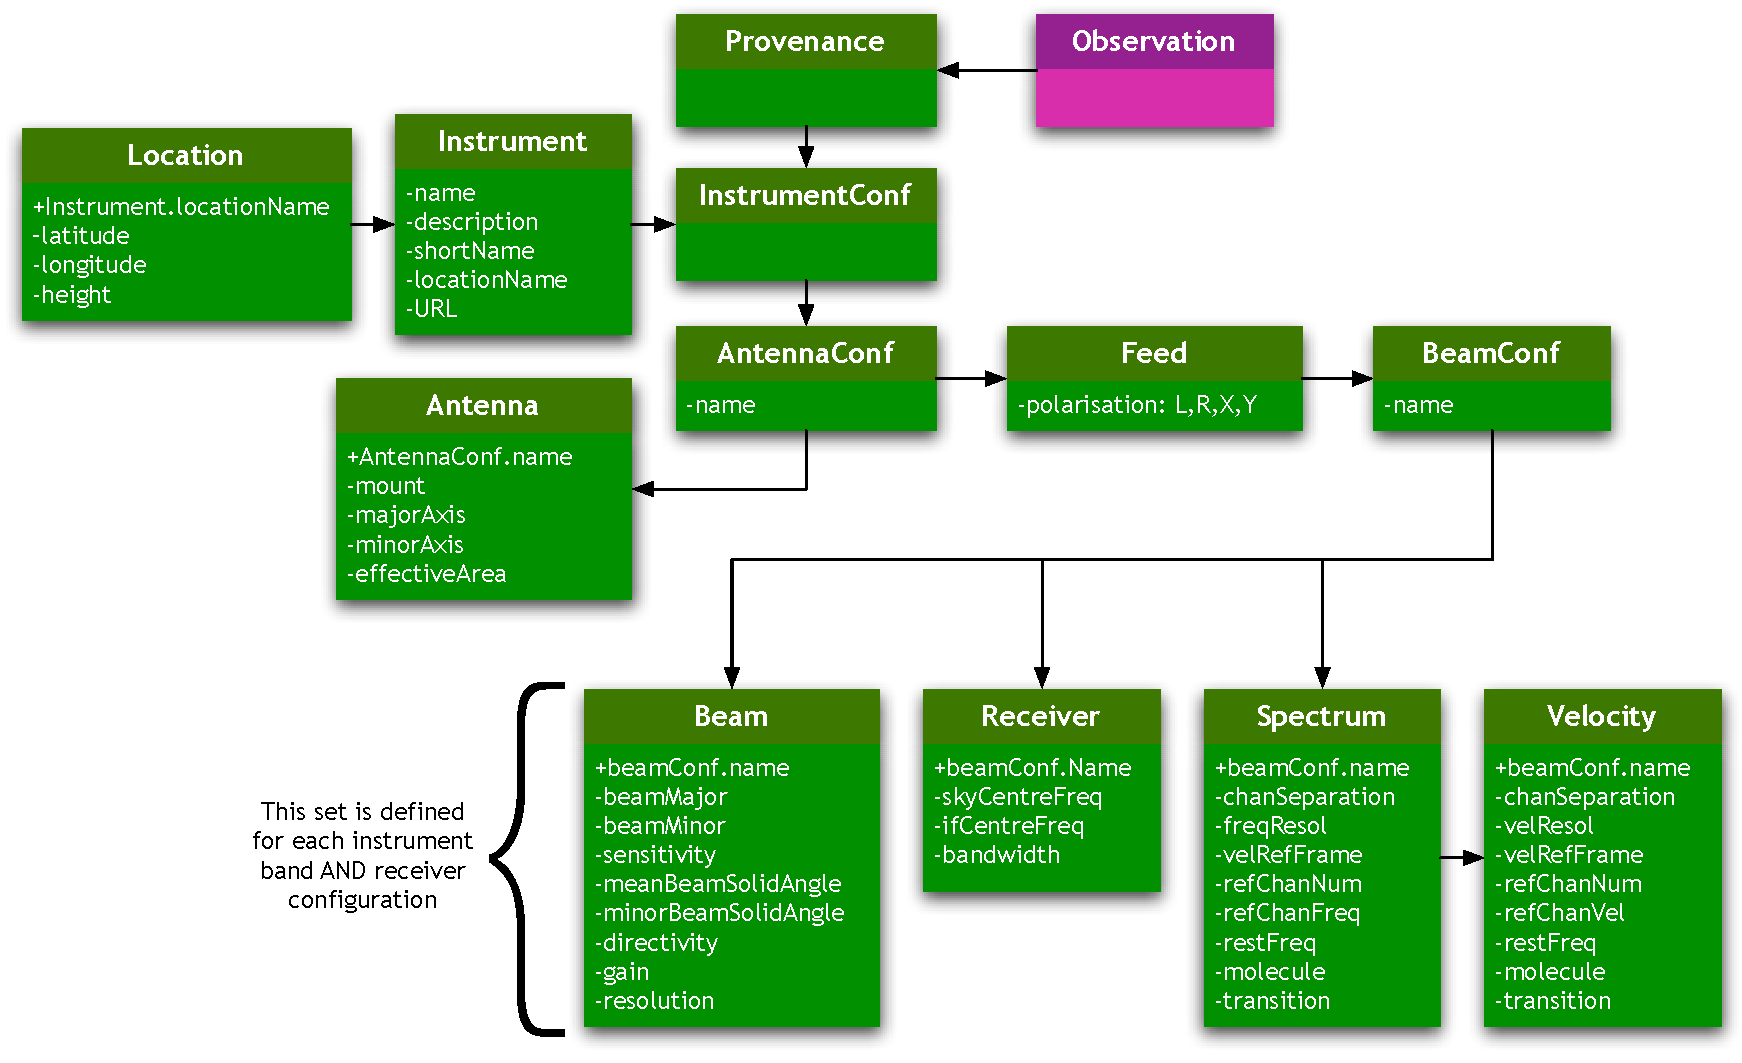
\includegraphics[width=\columnwidth]
		{fig/Provenance-Instrument-DM}
		\end{center}
		\caption[Provenance.Instrument data model]
		{Provenance.Instrument data model.}
		\label{figProvenanceInstrument}
		\end{figure}
		
		\begin{description}
			\item[InstrumentConf] Each observation is associated to
			a particular instrumental configuration, which results
			from the particular configuration of the instrument +
			antenna + feed system. InstrumentConf instances group
			those settings.
			
			 \item[Instrument] Instances of this class specify the
			instrument configuration, as used for the observation.
			
			 \item[Instrument.Location] This is an instance of a
			Location class, used for specifying the location for
			the instrument.
			
			 \item[AntennaConf] In the same way InstrumentConf
			allows the grouping for all the instrumental settings,
			AntennaConf instances group together Antenna and Feed
			info (regarding polarisation), plus BeamConf ---another
			aggregator class---. Several AntennaConf instances
			can provide information for different antennas and
			feeds. Each possible antenna configuration will be
			labelled by a name.
			
			 \item[Antenna] Instances of this class specify the
			general properties for each given antenna. We will also
			use these instances to specify the type of scan being
			performed on the source from a controlled vocabulary.
			
			 \item[Feed] Instances of this class ---one or more per
			AntennaConf--- specify each of the feed horns used for
			the observation, and their corresponding polarisation
			from a controlled vocabulary: \texttt{L}, \texttt{R},
			\texttt{X}, \texttt{Y}. We cannot make use of the
			Stokes polarisation parameters, as they cannot be
			directly measured via the feed configuration: instead,
			they have to derived by means of data processing steps.
			
			 \item[BeamConf] This class is used to group antennas,
			feeds, and beams. The relationship between BeamConf and
			Feed instances allows the specification of different
			beams, formed by the combination of different feeds. In
			a single-dish single-feed configuration, there is only
			one beam associated to a given receiver. We can also
			use this association for a single-dish, multiple-feed
			configuration where each feed goes to a different
			receiver.
			
			 \item[Beam] Metadata for this class specifies the
			actual beam for the telescope, associated to a given
			spectral band.
			
			 \item[Receiver] This metadata are used to describe the
			most relevant properties of the receiver, such as
			receiver type, intermediate frequency ---in the case of
			heterodyne stages---, et cetera.
			
			 \item[Spectrum] In case of spectroscopic observations,
			the spectral analyser that has been used is specified
			by instances of this class.
			
			 \item[Velocities] This class mirrors the Spectrum
			class, and is preferred for those cases where
			velocities are used, instead of frequency.
		\end{description}

		\begin{table}
		\caption[Provenance instrument metadata]
		{Provenance instrument metadata.}
		\begin{smallertabular}{p{2.15 cm}p{1.5cm}p{2.25cm}p{5.35cm}}
			& \textbf{FITS} & & \\ \textbf{Attribute} &
            \textbf{Keyword} & \textbf{UCD} & \textbf{Description}\\
            \midrule name & \texttt{INSTRUME} & \texttt{meta.id; instr;
            meta.main} & Instrument name.\\ \addlinespace description &
            \texttt{assign} & \texttt{meta.note; meta.main} &
            Instrument description.\\ \addlinespace shortName &
            \texttt{assign} & \texttt{instr; meta.id} & Short name for
            the instrument.\\ \addlinespace locationName &
            \texttt{assign} & \texttt{instr; pos; meta.id} &
            Localisation of the instrument.\\ \addlinespace URL &
            \texttt{COMMENT} & \texttt{instr; meta.ref.url} & URL for
            the instrument (website for the instrument, documentation,
            or any other type of instrument description).\\
            \addlinespace
		\end{smallertabular}
		\label{tabProvenanceInstrument}
		\end{table}

		\begin{table}
		\caption[Instrument location metadata]
		{Instrument location metadata.}
		\begin{smallertabular}{p{2 cm}p{1.5cm}p{3.2cm}p{4.55cm}}
					& \textbf{FITS} & & \\ \textbf{Attribute} &
		            \textbf{Keyword} & \textbf{UCD} & \textbf{Description}\\
		            \midrule locationName & \texttt{assign} &
		            \texttt{instr; pos; meta.id} & Name of a particular
		            instrument location.\\ \addlinespace latitude & \texttt{SITELAT}
		            & \texttt{instr; pos.earth.lat} & Instrument location
		            latitude.\\ \addlinespace longitude & \texttt{SITELONG} &
		            \texttt{instr; pos.earth.lon} & Instrument location
		            longitude.\\ \addlinespace altitude & \texttt{SITEELEV} &
		            \texttt{instr; pos.earth.altitude} & Instrument location
		            altitude.\\ \addlinespace
		\end{smallertabular}
		\label{tabProvenanceInstrLocation}
		\end{table}

		\begin{table}
		\caption[Antenna configuration metadata]
		{Antenna configuration metadata.}
		\begin{smallertabular}{p{2 cm}p{1.5cm}p{3.2cm}p{4.55cm}}
					& \textbf{FITS} & & \\ \textbf{Attribute} &
		            \textbf{Keyword} & \textbf{UCD} & \textbf{Description}\\
		            \midrule name & \texttt{assign} & \texttt{instr.telescope;
		            meta.title; meta.id} & Name of the particular antenna.\\
		            \addlinespace scanType & \texttt{assign} &
		            \texttt{instr.setup; meta.code} & Type of scan being
		            performed by this antenna, from a limited vocabulary
		            (suggested by the RDM \cite{LamPow0310IVOA}):
		            \texttt{beam\-Switch}, \texttt{cal}, \texttt{cross},
		            \texttt{dop\-pler\-Track}, \texttt{dwell},
		            \texttt{fo\-cus}, \texttt{fre\-quen\-cy\-Switch},
		            \texttt{hol\-og\-ra\-phy}, \texttt{mo\-sa\-ic},
		            \texttt{on\-Off}, \texttt{on\-The\-Fly}, \texttt{point},
		            \texttt{pos\-i\-tion\-Switch}, \texttt{pul\-sar},
		            \texttt{ras\-ter}, \texttt{sky\-Dip}, \texttt{tiedArray},
		            \texttt{track}, \texttt{wob\-bler\-Switch}.\\ \addlinespace
		            mount & \texttt{assign} & \texttt{meta.note} & Mount type
		            for the telescope from a limited vocabulary:
		            \texttt{azimuthal}, \texttt{e\-qua\-to\-ri\-al},
		            \texttt{alt\-az\-i\-muth\-al}, \texttt{dobson},
		            \texttt{german e\-qua\-to\-ri\-al}.\\ \addlinespace
		            majorAxis & \texttt{assign} & \texttt{instr;
		            phys.size.smajAxis} & Major axis dimensions.\\
		            \addlinespace minorAxis & \texttt{assign} & \texttt{inst;
		            phys.size.sminAxis} & Minor axis dimensions.\\
		            \addlinespace effectiveArea & \texttt{assign} &
		            \texttt{instr; phys.area} & Effective instrument area.\\
		            \addlinespace
		\end{smallertabular}
		\label{tabProvenanceInstrAntenna}
		\end{table}

		\begin{table}
		\caption[Feed configuration metadata]{Feed configuration metadata.}
		\begin{smallertabular}{p{2 cm}p{1.5cm}p{3.2cm}p{4.55cm}}
					& \textbf{FITS} & & \\ \textbf{Attribute} &
		            \textbf{Keyword} & \textbf{UCD} & \textbf{Description}\\
		            \midrule polarisation & \texttt{STOKES} &
		            \texttt{pos.posAng; phys.polarization; meta.code} &
		            Polarisation value from a controlled vocabulary:
		            \texttt{L}, \texttt{R}, \texttt{X}, \texttt{Y}\\
		            \addlinespace
		\end{smallertabular}
		\label{tabProvenanceInstrFeed}
		\end{table}

		\begin{table}
		\begin{minipage}{\linewidth}
		\caption[Beam configuration metadata]{Beam configuration metadata.}
		\begin{smallertabular}{p{3 cm}p{1.5cm}p{3.35cm}p{3.40cm}}
					& \textbf{FITS} & & \\ \textbf{Attribute} &
		            \textbf{Keyword} & \textbf{UCD} & \textbf{Description}\\
		            \midrule beamMajor & \texttt{BMAJ/HPBW} &
		            \texttt{instr.beam; phys.size.smajAxis} & Major axis HPBW
		            of the main lobe of the beam.\\ \addlinespace beamMinor &
		            \texttt{BMIN/HPBW} & \texttt{instr.beam;
		            phys.size.sminAxis} & Minor axis HPBW of the main lobe of
		            the beam.\\ \addlinespace sensitivity & \texttt{BEAMEFF} &
		            \texttt{instr.beam; instr.sensitivity} & Beam average
		            sensitivity.\\ \addlinespace mainBeamSolidAngle &
		            \texttt{assign} & \texttt{instr.beam; pos.posAng;
		            meta.main} & Main lobe’s beam solid angle.\\ \addlinespace
		            totalBeamSolidAngle & \texttt{assign} &
		            \texttt{instr.beam; pos.posAng; stat.max} & Total beam
		            solid angle, including secondary lobes.\\ \addlinespace
		            directivity & \texttt{assign} & \texttt{instr.beam;
		            instr.setup; arith.factor} & Directivity percentage.\\
		            \addlinespace gain & \texttt{ANTGAIN} & \texttt{instr.beam;
		            instr.setup; arith.factor} & Beam gain\footnote{We still
		            have to clarify if the gain attribute is related to the
		            directivity concept or not, and if it is related with the
		            receiving stages or not.}.\\ \addlinespace
		\end{smallertabular}
		\label{tabProvenanceInstrBeam}
		\end{minipage}
		\end{table}

		\begin{table}
		\caption[Receiver metadata]{Receiver metadata.}
		\begin{smallertabular}{p{2.15 cm}p{1.5cm}p{2.35cm}p{5.25cm}}
					& \textbf{FITS} & & \\ \textbf{Attribute} &
		            \textbf{Keyword} & \textbf{UCD} & \textbf{Description}\\
		            \midrule type & \texttt{BACKEND} &
		            \texttt{instr.setup; meta.note} & Receiver type (HEMT,
		            Bolo\-meter, SIS,
					et cetera).\\ \addlinespace skyCentreFreq & \texttt{assign} &
		            \texttt{src; em.radio; em.freq} & Antenna tuning
		            frequency.\\ \addlinespace IFCentreFreq & \texttt{assign} &
		            \texttt{instr.setup; em.freq} & Heterodyne receiver
		            intermediate frequency (or list of frequencies).\\ \addlinespace
		            bandwidth & \texttt{BANDWID} & \texttt{instr.bandwidth} &
		            Filter-bank total bandwidth.\\ \addlinespace
		\end{smallertabular}
		\label{tabProvenanceInstrReceiver}
		\end{table}

		\begin{table}
		\begin{minipage}{\linewidth}
		\caption[Spectrum metadata]
		{
			Spectrum metadata. It might be necessary to change the
		    \texttt{MOLECULE} and \texttt{TRANSITI} keywords by
		    \texttt{LINE}, for better CLASS compatibility.
		}
		\begin{smallertabular}{p{2 cm}p{1.5cm}p{3.4cm}p{4.35cm}}
					& \textbf{FITS} & & \\ \textbf{Attribute} &
		            \textbf{Keyword} & \textbf{UCD} & \textbf{Description}\\
		            \midrule numChannels & \texttt{NAXISn} &
		            \texttt{spect; em.freq; meta.number} & Number of spectral
		            channels.\\ \addlinespace chanSeparation\footnote{There is a
		            certain redundancy between the
		            Provenance.Spectrum.chanSeparation attribute and the
		            Coverage.Spectral.Resolution attributes.} &
		            \texttt{assign} & \texttt{spect; em.freq} & Mean channel
		            separation (in frequency units), or channel frequency
		            separation array.\\ \addlinespace freqResolution &
		            \texttt{FREQRES} & \texttt{spect.resolution; em.freq} &
		            Frequency resolution.\\ \addlinespace refChanNum &
		            \texttt{assign} & \texttt{spect; em.freq; meta.number;
		            meta.ref} & Spectral reference channel.\\ \addlinespace
		            refChanFreq & \texttt{OBSFREQ } & \texttt{spect; em.freq;
		            meta.code; meta.ref} & Spectral reference frequency
		            (observed frequency).\\ \addlinespace restFreq & \texttt{FREQn}
		            or \texttt{RESTFREQ} & \texttt{spect.line; em.freq} &
		            Observed spectral line rest frequency.\\ \addlinespace molecule
		            & \texttt{MOLECULE}\footnote{It might be necessary to
		            change the \texttt{MOLECULE} keyword by \texttt{LINE},
		            for better CLASS compatibility.} & \texttt{spect;
		            phys.mol; meta.id} & Molecule name.\\ \addlinespace transition &
		            \texttt{TRANSITI}\footnote{It might be necessary to
		            change the \texttt{TRANSITI} keyword by \texttt{LINE},
		            for better CLASS compatibility.} & \texttt{spect;
		            phys.atmol.transition; meta.id} & Transition.\\ \addlinespace
		\end{smallertabular}
		\label{tabProvenanceInstrSpectrum}
		\end{minipage}
		\end{table}

		\begin{table}
		\begin{minipage}{\linewidth}
		\caption[Velocity metadata]{Velocity metadata.}
		\begin{smallertabular}{p{2 cm}p{1.5cm}p{3.4cm}p{4.35cm}}
				& \textbf{FITS} & & \\ \textbf{Attribute} & \textbf{Keyword} &
		        \textbf{UCD} & \textbf{Description}\\ \midrule numChannels
		        & \texttt{assign} & \texttt{spect; phys.veloc; meta.number} &
		        Number of velocity channels.\\ \addlinespace
		        chanSeparation\footnote{There is a certain redundancy between
		        the Provenance.Velocity.chanSeparation attribute and the
		        Coverage.Spectral.Resolution attributes.} & \texttt{assign} &
		        \texttt{spect; phys.veloc} & Mean channel separation (in
		        velocity units), or velocity channel separation array.\\ \addlinespace
		        velResolution & \texttt{assign} & \texttt{spect.resolution;
		        phys.veloc} & Velocity resolution.\\ \addlinespace velRefFrame &
		        \texttt{assign} & \texttt{spect; phys.veloc; pos.frame;
		        meta.id} & Identification of the reference system used for the
		        velocity.\\ \addlinespace refChanNum & \texttt{assign} &
		        \texttt{spect; phys.veloc; meta.number; meta.ref} & Velocity
		        reference channel.\\ \addlinespace refChanFreq & \texttt{assign } &
		        \texttt{spect; phys.veloc; meta.code; meta.ref} & Frequency for
		        the velocity reference channel.\\ \addlinespace restFreq &
		        \texttt{RESTFREQ} & \texttt{spect.line; em.freq} & Observed
		        spectral line rest frequency.\\ \addlinespace molecule &
		        \texttt{MOLECULE}\footnote{It might be necessary to change the
		        \texttt{MOLECULE} keyword by \texttt{LINE}, for better CLASS
		        compatibility.} & \texttt{spect; phys.mol; meta.id} & Molecule
		        name.\\ \addlinespace transition & \texttt{TRANSITI}\footnote{It might
		        be necessary to change the \texttt{TRANSITI} keyword by
		        \texttt{LINE}, for better CLASS compatibility.} &
		        \texttt{spect; phys.atmol.transition; meta.id} & Transition.\\
		        \addlinespace
		\end{smallertabular}
		\label{tabProvenanceInstrVelocity}
		\end{minipage}
		\end{table}
		
	% section instrumental_provenance (end)
	
	\section{Environmental provenance} % (fold)
	\label{sec:environmental_provenance}
		
		Environmental provenance is the part of the provenance
		dealing with ambient conditions, and as such the main class
		is called Provenance.AmbientConditions: it encompasses all
		metadata needed to specify weather conditions, air mass, 
		opacity, et cetera. Figure
		\ref{figProvenanceAmbient} shows the corresponding classes and
		their relationships.

		\begin{figure}[tbp]
		\begin{center}
		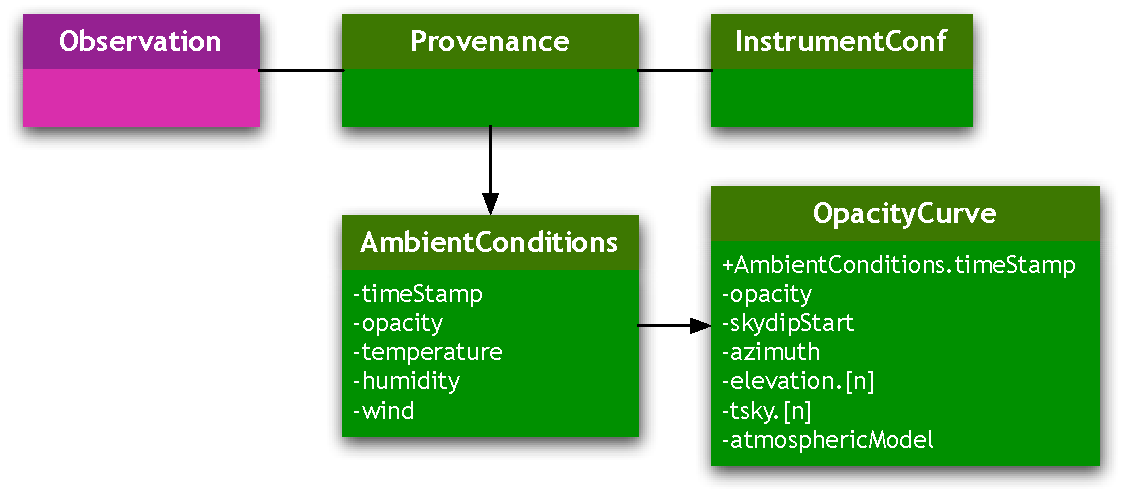
\includegraphics[width=\columnwidth]
			{fig/Provenance-AmbientConditions-DM}
		\end{center}
		\caption[Provenance.AmbientConditions data model]
			{Provenance.AmbientConditions data model.}
		\label{figProvenanceAmbient}
		\end{figure}
		
		
		\begin{description}
			\item[AmbientConditions] Holds all metadata related
			with weather conditions for the observation, such as
			humidity, wind speed, opacity at zenith, et cetera.
			
			 \item[OpacityCurve] Includes the opacity curve (linked
			as a VOTable file) associated to the observing term
			where the data were observed (which we will derive from
			the nearest two skydip scans performed before and after
			the observation). We propose the inclusion of an array
			of \texttt{[elevation, Tsky]} pairs, together with the
			azimuth and the starting time of the skydip.
			Calculation of the opacity curve is different for
			bolometric or heterodyne observations. It is also
			necessary to include information on the atmospheric
			model and/or software used for opacity fitting (the
			atmospheric model used by MOPSIC and MIRA,
			the data reduction packages at the IRAM~30m antenna,
			is the \emph{Atmospheric Transmission at Microwaves},
			ATM, by Pardo et al.~\cite{ParCerSer01Atmospheric}).
		\end{description}
		

		\begin{table}
		\caption[AmbientConditions metadata]{AmbientConditions metadata.}
		\begin{smallertabular}{p{1.65 cm}p{2.75cm}p{3.25cm}p{3.60cm}}
				& \textbf{FITS} & & \\ \textbf{Attribute} & \textbf{Keyword} &
		        \textbf{UCD} & \textbf{Description}\\ \midrule opacity &
		        \texttt{TAUZEN} & \texttt{phys.absorption.coeff} & Opacity at
		        zenith estimated at the observation frequency.\\ \addlinespace airMass
		        & \texttt{AIRMASS} & \texttt{obs.airMass} & Air mass at zenith
		        at the observing site.\\ \addlinespace temperature & \texttt{TAMBIENT}
		        & \texttt{phys.temperature} & Ambient temperature.\\ \addlinespace
		        humidity & \texttt{HUMIDITY} & \texttt{obs.atmos;
		        phys.columnDensity} & Ambient humidity.\\ \addlinespace waterVapour &
		        \verb+TAU_WPATH_RD<freq>+ & \texttt{obs.atmos; phys.pressure} &
		        Equivalent pressure of the water vapour column.\\ \addlinespace
		        tauFrequency & \verb+TAU_WPATH_RD<freq>+ & \texttt{obs.atmos;
		        em.freq} & Tau radiometer frequency.\\ \addlinespace wind &
		        \texttt{WINDSPEE} & \texttt{obs.atmos; phys.veloc} & Wind
		        speed.\\ \addlinespace
		\end{smallertabular}
		\label{tabProvenanceAmbientConditions}
		\end{table}

		\begin{table}
		\caption[Opacity metadata]{Opacity metadata.}
		\begin{smallertabular}{p{1.85 cm}p{1.5cm}p{3.4cm}p{4.5cm}}
				& \textbf{FITS} & & \\ \textbf{Attribute} & \textbf{Keyword} &
		        \textbf{UCD} & \textbf{Description}\\ \midrule opacity &
		        \texttt{TAUZEN} & \texttt{phys.absorption.coeff} & Opacity at
		        zenith estimated at the observation frequency.\\ \addlinespace
		        skydipStart & \texttt{DATE-OBS} & \texttt{time.obs.start} &
		        Skydip starting time.\\ \addlinespace azimuth & \texttt{AZIMUTH} &
		        \texttt{pos.az} & Skydip azimuth.\\ \addlinespace elevation[n] &
		        \texttt{ELEVATIO} & \texttt{pos.el} & Skydip scan elevation.\\
		        \addlinespace tsky[n] & \texttt{assign} & \texttt{instr.skyTemp} & Sky
		        temp at $\mathrm{n^{th}}$ skydip.\\ \addlinespace atmosModel &
		        \texttt{assign} & \texttt{meta.modelled; obs.atmos; meta.id} &
		        Atmospheric model identification.\\ \addlinespace
		\end{smallertabular}
		\label{tabProvenanceAmbientOpacity}
		\end{table}
		
		
	% section environmental_provenance (end)
	
	\section{Processing provenance} % (fold)
	\label{sec:processing_provenance}
		
		The Provenance.Processing class will enable the
		specification of processing processes applied to the data
		before archival, including some processes necessary for the
		actual observation, such as the determination of the
		background signal via \texttt{frequencySwitching} or
		\texttt{positionSwitching} for background/source data
		comparison.
		
		 The RADAMS will make use of just two classes, Processing
		and Calibration ---this is a subclass of processing---.
		Order is relevant, and it should be possible to reconstruct
		the pipeline by the ordering of Processing and/or
		Calibration instances. Figure \ref{figProvenanceProcessing}
		shows these classes.

		\begin{figure}[tbp]
		\begin{center}
		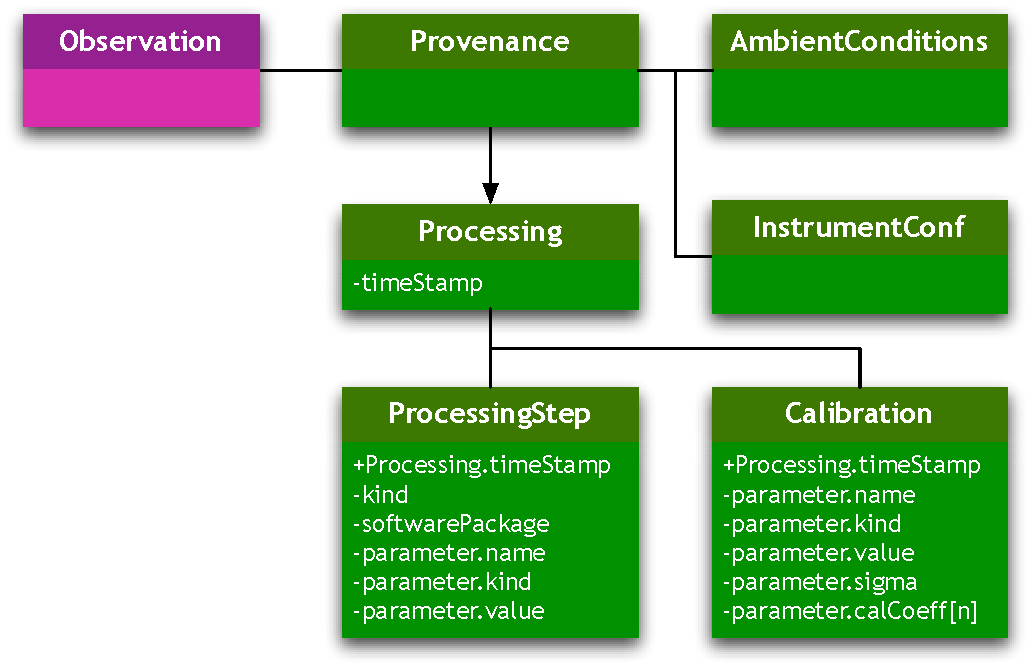
\includegraphics[width=0.6\columnwidth]{fig/Provenance-Processing-DM}
		\end{center}
		\caption[Provenance.Processing data model]
			{Provenance.Processing data model.}
		\label{figProvenanceProcessing}
		\end{figure}
		
		\begin{description}
			\item[Processing] It holds information specifying the
			type of processing applied to data before archival.
			This includes pseudo-observational techniques such as
			position switching or frequency switching, as well as
			the type of data averaging, data weighting, et cetera.
			Table \ref{tabProvenanceProcessingStep} provides
			minimal initial metadata, using arrays of parameter
			keywords for extensibility at the expense of
			complexity.
			
			 \item[Calibration] It is a subclass of Processing,
			where the type of processing is dataCalibration. In
			this class there are additional attributes to specify
			the type of calibration, and the axes to where this
			calibration will be applied. Table
			\ref{tabProvenanceCalibration} provides minimal initial
			metadata, using arrays of parameter keywords for
			extensibility at the expense of complexity.
		\end{description}
		
		 We still have to develop a calibration and/or pointing
		model; maybe based upon IRAM-Multi-Beam-FITS, or GBT FITS
		calibration tables.

		\begin{table}
		\begin{minipage}{\linewidth}
		\caption[Processing Step]{Processing Step metadata.}
		\begin{smallertabular}{p{2.75 cm}p{1.5cm}p{2.25cm}p{4.75cm}}
				& \textbf{FITS} & & \\ \textbf{Attribute} & \textbf{Keyword} &
		        \textbf{UCD} & \textbf{Description}\\ \midrule timestamp &
		        \texttt{DATE-RED} & \texttt{obs.param; time.epoch} & Timestamp
		        for the processing step being performed.\\ \addlinespace type &
		        \texttt{assign} & \texttt{obs.param; meta.code} & Type of
		        processing applied to source data; comes from a controlled
		        vocabulary: \texttt{un\-proc\-essed},
		        \texttt{noise\-Weight\-ed\-Av\-er\-age},
		        \texttt{non\-Weight\-ed\-Av\-er\-age}.\\ \addlinespace
		        software\-Package & \texttt{assign} & \texttt{meta.software;
		        meta.id} & Software package used for data processing; should
		        come from a controlled vocabulary: \texttt{CLASS},
		        \texttt{AIPS}, \texttt{AIPS++}, \texttt{CASA}, \texttt{MOPSIC},
		        \texttt{GILDAS}, \texttt{MIRA}, \texttt{MIR}, \texttt{other}.
		        In the case of \texttt{other}, the actual package that was used
		        should be added as a parameter, with parameter.name as
		        \texttt{software\-Package} and the parameter.value as the
		        package name. \\ \addlinespace parameter[n].name & \texttt{assign} &
		        \texttt{obs.param; meta.code} & Additional processing parameter
		        name, whose value will be in parameter.value; eventually, we
		        will have a controlled list of possible parameter.name
		        values.\\ \addlinespace parameter[n].type & \texttt{assign} &
		        \texttt{obs.param; meta.code} & From a controlled vocabulary:
		        \texttt{integer}, \texttt{float}, \texttt{string}, et cetera.
				At least all
		        of FITS data types should be present.\\ \addlinespace
		        parameter[n].value & \texttt{assign} &
		        \texttt{obs.param}\footnote{The final UCD to mark
		        parameter[n].value will be calculated when writing the VOTable,
		        as it depends on parameter.type; it will be \texttt{obs.param;
		        meta.number} most of the time, but it could be
		        \texttt{obs.param; meta.name} or \texttt{obs.param; meta.code},
		        depending on the context.} & Value for the parameter indicated
		        by parameter.name.\\ \addlinespace
		\end{smallertabular}
		\label{tabProvenanceProcessingStep}
		\end{minipage}
		\end{table}

		\begin{table}
		\begin{minipage}{\linewidth}
		\caption[Calibration metadata]
		{
			Calibration metadata\footnote{It is mandatory that at least one
			\texttt{[parameter.name, parameter.type, parameter.value]}
			triplet appears, with \texttt{fluxScale} as parameter.name, and
			one of \texttt{antennaTemperature},
			\texttt{mbBrightnessTemperature}, or \texttt{S\_nu} as the
			parameter.value, with a parameter.type of \texttt{string}.}.
		}
		\begin{smallertabular}{p{3.15 cm}p{1.5cm}p{2.0cm}p{4.60cm}}
				& \textbf{FITS} & & \\ \textbf{Attribute} & \textbf{Keyword} &
		        \textbf{UCD} & \textbf{Description}\\ \midrule timestamp &
		        \texttt{DATE-RED} & \texttt{obs.param; time.epoch} & Timestamp
		        for the calibration step being performed.\\ \addlinespace
		        parameter.name & \texttt{assign} & \texttt{obs.calib;
		        obs.param; meta.id} & Keyword defining the parameter that we
		        will characterise with the remaining attributes.\\
		        \addlinespace parameter.type & \texttt{assign} &
		        \texttt{obs.calib; obs.param; meta.code} & Type of calibration
		        parameter used, from a controlled vocabulary:
		        \texttt{additive}, \texttt{fac\-tor}, \texttt{pol\-y\-no\-mi\-al},
		        \texttt{ex\-po\-nen\-tial}, \texttt{log\-a\-rith\-mic}.\\
		        \addlinespace parameter.value & \texttt{assign} &
		        \texttt{obs.calib; obs.param; meta.number} & Value for the main
		        calibration parameter, where parameter.type is not
		        \texttt{polynomial}.\\ \addlinespace parameter.sigma &
		        \texttt{assign} & \texttt{obs.calib; obs.param; meta.number} &
		        Value of sigma, for \texttt{exponential} calibrations.\\
		        \addlinespace parameter.calCoeff.[n] & \texttt{assign} &
		        \texttt{obs.calib; obs.param; meta.number} & $\mathrm{n^{th}}$
		        degree coefficient for a \texttt{polynomial} calibration
		        parameter; polynomial degree is derived from the maximum n.\\
		        \addlinespace
		\end{smallertabular}
		\label{tabProvenanceCalibration}
		\end{minipage}
		\end{table}
		
		
	% section processing_provenance (end)
	
	
	\section{Conclusions} % (fold)
	\label{sec:data_provenance_conclusions}
		
		With this chapter we have finished our task of defining
		the modules suggested for the ObsDM, with the objective
		of being able to create a complete data model which
		could be used as a blueprint for archive development.
		
		The Provenance data model is the most instrument dependant
		of the RADAMS models, but of the three sub-models, only
		the Instrument part is strictly specific to radio astronomy.
		This is a strength, however, as the Environment and 
		Processing can be considered part of the atmosphere, and
		part of the workflow, and they are equally needed for all
		kinds of observations. By having the Instrument specific
		signature encapsulated in the Provenance.Instrument
		sub-model, it can be replaced by different
		Provenance.Instrument descriptions, 
		meaningful for the different data analysis packages, which
		are the ones that need the instrument-specific
		information.
	
		
		
	% section data_provenance_conclusions (end)
	
% chapter radams_data_provenance (end)
	% 	\chapter{Conclusions} % (fold)
	\label{cha:radio_data_modelling_conclusions}

	\todo{
		\begin{itemize}
			\item Data modelling in the VO, necessary for
			interoperability.
			
			\item Existing VO data models, still incomplete in several
			particular models, specially in radio astronomy, but also
			for general astronomy and astrophysics.
			
			\item Our Provenance data model is a necessary addition for
			radio astronomy, and a useful addition for general
			astronomy.
		\end{itemize}
	}
	
%	El cuadrado de una suma corresponde al cuadrado del primer término,
%	más el doble producto del primer término por el segundo, más el
%	cuadrado del segundo:
%
%	\begin{align}
%	 (x+y)^2 &=  (x+y)(x+y)				\label{step1} \\
%	         &=  (x+y)x + (x+y)y		\label{step2} \\
%	         &=  x^2 + yx + xy + y^2	\label{step3} \\
%	         &=  x^2 + xy + xy + y^2	\label{step4} \\
%	         &=  x^2 + 2xy + y^2		\label{step5} 
%	\end{align}
%
%	Veamos cada una de estas transformaciones en detalle, para ver de
%	qué propiedades nos estamos valiendo en cada una:
%
%	\begin{description}
%		\item[Transformación \eqref{step1}]  el cuadrado de un elemento
%	          algebraico, es el producto de ese elemento por sí mismo.
%
%		\item[Transformación \eqref{step2}]  propiedad distributiva 
%			  del primer elemento sobre la suma del segundo.
%
%		\item[Transformación \eqref{step3}]  propiedad distributiva de
%		      los productos que quedaban.               
%                                          
%		\item[Transformación \eqref{step4}]  propiedad conmutativa para
%		      reordenar monomios.                   
%                                          
%		\item[Transformación \eqref{step5}]  agrupación de monomios
%		      semejantes.
%	\end{description}
	
	% chapter radio_data_modelling_conclusions (end)

	
	% part VO data models (end)
	
	% part accessingRadioVOdata (fold)
	\part{Bringing legacy tools to the VO}
	\label{prt:legacyTools}
	
	%2345678901234567890123456789012345678901234567890123456789012345678901

% chapter cha:using_legacy_tools (fold)
\chapter[Legacy astronomical packages and the VO]
{Legacy astronomical packages and the VO}
\label{cha:using_legacy_tools}
	\attributedquote{
		\dictionarydef{legacy}
					  {noun}
		{
			\begin{itemize}
				\item a thing handed down by a predecessor:
				\emph{the legacy of centuries of neglect.}
			\end{itemize}
		}
		\dictionarydef{legacy}
					  {adjective (\textsf{computing})}
		{
			\begin{itemize}
				\item Denoting software or hardware that has been
				superseded but is difficult to replace because of
				its wide use.
			\end{itemize}
		}
	}
	{The New  Oxford American Dictionary, \emph{2nd Edition}}
	
	The physical properties we can ascertain from remote
	astronomical objects are the result of careful computations on
	observed datasets, which tend to be observatory, telescope,
	instrument, and even observing mode specific. Such computations
	include background noise estimations, electron counts to
	incident flux conversions, instrument signal removal, et
	cetera.

	Many different software packages have been developed for
	performing those operations (which are commonly known as data
	reduction), and obtaining science-ready data products (i.e.,
	images which have been flux calibrated, given precise
	astrometry, et cetera), and to analyse them to get additional
	physical information. For instance, once a spectrum has been
	calibrated on the local standard of rest of the source,
	the width of an emission line can be directly correlated to
	an expansion or contraction velocity of the observed object.
	
	The development effort invested on these applications is
	enormous, and even when they have been developed using
	techniques available many years ago, and can be considered
	\emph{technologically obsolete}, the recreation of all the
	algorithms in modern languages, or on more modern GUI framework
	foundations is prohibitive, due to the extensive development
	and testing that would be needed for such a replacement.
	
	Examples of 30-year old software packages still in heavy use
	include AIPS\urlnote{http://www.aips.nrao.edu/}, a radio
	astronomical imaging package from the late seventies originally
	written in FORTRAN IV; or
	GIPSY\urlnote{http://www.astro.rug.nl/~gipsy/}, a 3D data
	analysis package for obtaining kinematic properties, whose
	development started in the early seventies, and is also written
	in FORTRAN.
	
	But the goal set for the VO is to become the entire framework
	for future astronomical and astrophysical computing, both for
	its development and its execution, becoming completely
	transparent to astronomical users.
	
	\invisiblenote{
		Talking about the Virtual Observatory will be left to
		computer scientists or astronomical software developers,
		much in the same way the Internet has become \emph{the
		internet} (without capitalising), and web applications and
		web services use it. Web applications such as Google
		Docs\urlnote{http://docs.google.com/}, Yahoo!
		Mail\urlnote{http://mail.yahoo.com/},
		YouTube\urlnote{http://youtube.com/} and the like show an
		uniform interface to the user based on HTML4/XHTML and
		JavaScript which modern web browsers can uniformly render
		and access.
	}
	
	We cannot expect, then, astronomers to embrace the VO if they
	are not able to carry over the tools they are accustomed to,
	and we cannot recreate all the existing legacy applications. We
	must, therefore, find a way to bring these legacy applications
	to operate within the VO framework. That is the scope of this
	chapter: answering \emph{How to bring legacy applications into
	the VO environment.}
	
	\invisiblenote{
		However, there are many existing astronomical applications,
		written in the pre-internet era, many of them in languages
		which do not implement network connection primitives, such
		as FORTRAN\footnote{Network programming in FORTRAN is
		performed by means of wrappers around existing C
		libraries.}, in which many man-years have been invested,
		and which the astronomical community keeps on
		using\footnote{Examples of 30-year old software packages
		still in heavy use include AIPS
		<\url{http://www.aips.nrao.edu/}>, a radio astronomical
		imaging package from the late seventies originally written
		in FORTRAN IV; or GIPSY
		<\url{http://www.astro.rug.nl/~gipsy/}>, a 3D data analysis
		package for obtaining kinematic properties, developed in
		the early seventies, also written in FORTRAN.}.
		
		 In any case, VO capabilities are very desirable, as they
		enable software packages to find, select and process data
		which the application does not need \emph{a priori}
		knowledge of where they do reside: only the metadata in the
		VO Registry is needed for service selection, and only the
		metadata provided by actual protocol queries to the service
		allow \emph{a priori} selection of the final datasets to be
		processed.
		
		 \emph{How do we provide VO capabilities to existing
		(legacy) astronomical application in the least intrusive
		way?} That is the question we wish to answer with this
		chapter.
	}
	
	\section{VO-enabling applications} % (fold)
	\label{sec:vo_enabling_applications}
		
		We must start by answering the question \emph{What is a
		VO-enabled application?} From the many VO standards and
		protocols issued by the
		IVOA\urlnote{http://ivoa.net/Documents/}, which and how
		many of them have to be implemented for us to consider an
		application is VO-enabled?
		
		We will understand that a VO-enabled application is a
		software package which:
		
		\begin{enumerate}
			\item Can read and/or write data in VOTable (and
			possibly FITS) format.
			
			\item Can query the VO Registry in order to find
			VO services or data resources, at least of one
			particular kind.
			
			\item Can call a subset of VO-registered services
			for at least one of IVOA data access
			protocols\footnote{ConeSearch, Simple Image Access,
			or Simple Spectra Access. See 
			appendix~\ref{cha:vo_protocols}.}.
		\end{enumerate}
		
		A somehow orthogonal capability is that of being able to
		communicate with other VO applications running in the same
		machine, via the \invisible{soon to be approved} Simple
		Application Messaging Protocol
		(SAMP)~\cite{2009samp.ivoav0904T}.
		
		However, an application which can use SAMP to communicate
		with others can, in fact, make use of their capabilities, and
		retrieve data which have been processed by other applications. Conversely, the
		processed results can be mixed with those of any other
		application.
		
		We can, then, consider that a VO application is just one
		which:
		
		\begin{enumerate}
			\item Can read and/or write data in VOTable (and
			possibly FITS) format.
			
			\item Can communicate with other VO applications
			through messaging, both for sending and receiving
			data from those applications.
		\end{enumerate}
		
		As we are leaving out the Registry search capability, and
		protocol calls, in order to truly VO-enable an application
		we will need to ensure that VO Registry access services, and
		ways to call VO services, are provided.
		That can be solved by either implementing or using external
		modules which can query the registry, perform data access
		queries, and return their results back to processing
		applications.
		
		Let us compare, then, the two ways we have to create
		VO-enabled applications:
		
		\begin{description}
			\item[In-application VO compatibility] In this scenario,
			we have to create a VO interface within every
			application we want to VO-enable. The following has
			to be implemented:
			
			\begin{description}
				\item[VO Registry interface] A GUI for querying the
				VO registry, looking for the kind of services the
				application can make use of. Such a GUI can be
				reused only for applications using the same
				programming language and UI framework. We must
				consider it a \emph{per application} development.
				
				\item[Changes into the User Interface] The
				application user interface (be it command-line or
				graphical) has to be changed in order to be able to
				start the new VO functions: registry query,
				image/spectra/table queries and retrieval,
				messaging with other applications, et cetera. By
				definition, this is a \emph{per application}
				development.
				
				\item[VO Data Access Layer interface] The
				application must be able to obtain data from
				existing VO services (images, spectra, or tables).
				Code to query them must be included. There are
				query interfaces written in different programming
				languages, so we will consider this a \emph{per
				language} development.
				
				\item[VOTable and FITS handling] The two approved
				data formats for the VO are the VOTable and the
				FITS file formats. Any VO application has to be
				able to handle both (many VOTables include links to
				FITS files, which hold the actual data). There are
				libraries written for many different languages for
				FITS and VOTable handling, so there is a small
				\emph{per application} development cost associated.
				
				\item[DAL to internal model interface] Data
				retrieved from the VO correspond to the DAL data
				model, while the legacy application will have an
				internal data model of its own. This is responsible
				for the VOTable/FITS data conversion into the
				actual internal representation, and it is
				completely application dependendent, and as such it
				represents a \emph{per application} cost.
				
				\item[Messaging interface \emph{(optional)}] 
				The application can also include a messaging
				interface. In that case, the DAL to the internal
				data model interface is also used by the data being
				retrieved from other applications. The messaging
				interface is based on the
				XML-RPC\urlnote{http://www.xmlrpc.com/}
				specification~\cite{1999xrpc.rept.....W}, for which
				many implementations exist in many different
				languages. The adaptation between the DAL model and
				the internal model it is the same as for the VO
				query interfaces, and includes a small amount of
				\emph{per application} adaptation in order to
				support messaging.
			\end{description}
			
			
			\item[In-application VO messaging] In this other
			scenario, we leave the interface with the registry, and
			the DAL interface to other applications, and we rely on
			messaging to get the data in and out of the
			application. In this case, the modules to be
			implemented are:
			
			\begin{description}
				\item[Minimal changes to the UI (Views) and
				Controller] Applications must be able to send data
				to compatible VO applications (applications who
				understand the kind of messages the host
				application wishes to provide), and must declare
				the kind of messages it can receive from other
				applications. The main Controller must be able to
				receive updates from the Messaging part controller.
				
				\item[Messaging interface] In this case, messaging
				is the main building block for the application:
				other applications will perform the Registry
				queries, and the calls to data access protocols.
				The results will be later messaged to the
				application.
				
				\item[VOTable and FITS handling] The messaging
				protocols use VOTables, which can include links to
				FITS files, as any other VO protocol. As mentioned
				above, there are extensive libraries for many
				different languages which can be used. We can
				consider, also, that FITS handling is a capability
				of any legacy application, so only VOTable handling
				is a true addition.
				
				\item[DAL to internal model interface] This is
				interface can be simpler than the one in the prior
				scenario, because the data origins will be the
				messaging applications. As we will see later, the
				messaging protocols impose a more strict semantics
				to the data being exchanged, allowing for a simpler
				interface.
			\end{description} 
		\end{description}
		
		%\begin{figure}[tbp]
		%	\centering
		%		\includegraphics[height=3cm]
		%		{fig/StandardMVCarchitecture.pdf}
		%	\caption{caption}
		%	\label{fig:fig_StandardMVCarchitecture}
		%\end{figure}
		
		\begin{figure}[tbp]
			\centering
			\subfloat[][]
			{
				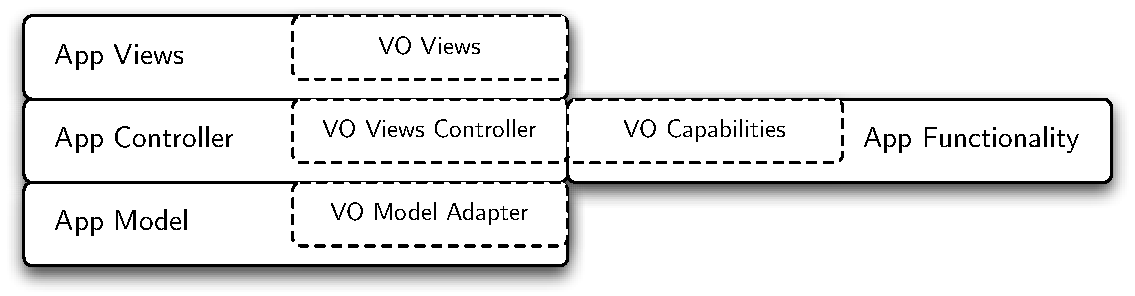
\includegraphics[width=\textwidth]
					{fig/VOappMVCarchitecture.pdf}
				%\label{fig:fig_VOappMVCarchitecture}
				\label{fig:fig_monolithic_VO}
			}
			\vfill
			\subfloat[][]
			{
				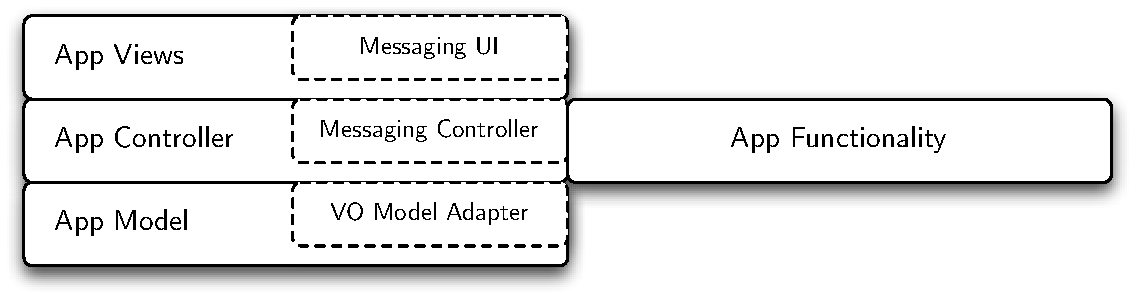
\includegraphics[width=\textwidth]
					{fig/MessagingMVCarchitecture.pdf}
				\label{fig:fig_modular_VO_capabilities}
			}
			\caption[Modules for monolithic a message-based VO-enabled
			applications]
			{
				Comparison between the functionality to be added
				and/or modified in a VO-enabled application, both
				for a monolithic approach
				\subref{fig:fig_monolithic_VO}, and for a
				messaging-based approach
				\subref{fig:fig_modular_VO_capabilities}.
			}
			\label{fig:monolithic_vs_modular_VO_capabilities}
		\end{figure}
		
		We can see these two different approaches illustrated in 
		figure~\ref{fig:monolithic_vs_modular_VO_capabilities}. 
		Figure~\ref{fig:fig_monolithic_VO} shows the monolithic
		approach to bringing legacy applications to the VO,
		with two different legacy applications and an already
		VO native application. We can see that there is a lot
		of redundancy and duplication in the development.
		
		Figure~\ref{fig:fig_modular_VO_capabilities}, on the other 
		hand, shows how a modular interface, which connects legacy
		applications via messaging protocols, decreases development
		effort, decouples the development of VO functionality, and
		provides tools which can be used with any VO messaging
		enabled application. If we assume that all legacy
		applications are able to handle FITS files, only messaging,
		VOTable handling, and DAL to internal data model
		modifications will have to be performed per application,
		while the interfaces to the VO, and all external, plug-in
		like, capabilities, can be left to external modules,
		common to all applications we might wish to update.
		
		There will be cases of applications where no modifications
		are possible, because no source code is available for them,
		or the language they are written in does not support
		web or XML-RPC interaction. In those cases, a VO downloader 
		application, ---which can act as a VO file consolidator---
		is the \emph{greatest common denominator}, and remains the
		only way to use non-VO enabled legacy applications within
		a VO workflow.
		
	% section vo_enabling_applications (end)
	
	\section{Inter-application messaging in the VO} % (fold)
	\label{sec:messaging_and_the_vo}
		
		In order to VO-enable applications through a messaging
		system,
		we wish to be able to send messages which entail particular
		actions: examples of messages and their actions would be:
		
		\begin{itemize}
			\item Issuing a \emph{data load} message, and having
			data loaded on the remote application.
			
			\item Issuing a \emph{highlight data} message, and
			have the data highlighted on the remote application.
		\end{itemize}
		
		Without taking into account the nature of the data (in 
		the VO, data is passed by means of VOTables, which might
		contain data, or link to data), it is clear that there
		might be several receivers for messages of this nature,
		so a mechanism for registering potential receivers of
		messages is needed. If the number of possible messages
		is moderate to large, an application would also need to
		declare the kind of messages it can deal with.
		
		We can see that a possible solution to this are
		publish-subscribe mechanisms, where several parties can
		act as information publishers, and several (possibly
		different) parties act as information subscribers.
		The benefits in scalability and modularity of
		publish/subscribe systems, together
		with a thorough study of their mechanisms, taxonomy, and
		predecessors, can be found in the review by
		Eugster et al.~\cite{857078}.
		
		The first messaging mechanism within the VO was an
		experiment by the VOTech project\footnote{In turn, inspired
		by the XPA (uniX Public Access,
		\url{http://hea-www.harvard.edu/RD/xpa/intro.html})
		protocol used for
		communication between tools written for the X11
		windowing system, or Tcl/Tk, or Perl packages, such as
		IRAF, or the SAOImage DS9 FITS
		viewer. IRAF, for instance, can use DS9 as its imaging
		package thanks to XPA.}, and was the PLatform for
		AStronomical Tool
		InterConnection\urlnote{http://plastic.sourceforge.net/}
		(PLASTIC)~\cite{2006pldaivoanv0606B}, a client-side
		messaging protocol.
		
		PLASTIC was based on XML-RPC messaging between client
		applications and a central hub which had to start before
		the applications could connect to it. Applications would
		register the messages they support, and would provide
		handler functions for incoming messages (callbacks).
		
		The number of defined messages was not very large, and
		by being implemented on top of XML-RPC it was easily
		ported to different languages and platforms. In fact,
		in spite of never being an IVOA standard, the number of
		applications supporting PLASTIC was very high, as the
		cost of implementing PLASTIC capabilities was very
		low.
		
		However, PLASTIC sported a number of shortcomings:
		
		\begin{description}
			\item[Hard-coded message types and parameters]
			The messages types were hard-coded in the protocol,
			making messages fixed, and not extensible. Small
			modifications to an existing message were not
			possible, as all parameters were fixed by the
			message definition.
			
			\item[Non-uniform messages] Each message had a
			number of parameters that depended entirely on
			the message type, without any governing rule.
			
			\item[Java-based typing] Data types were based on
			Java data types, instead of relying on
			platform-independent data type definitions.
			
			\item[Hard-coded transport type] PLASTIC uses
			XML-RPC as its transport protocol, making it
			impossible to use different messaging protocols
			if the need might arise (for instance, usage of
			SOAP, e-mail, or other kind of transfer protocol).
		\end{description}
		
		The answer to that was taking the best of PLASTIC, 
		which was never an IVOA standard, in spite of its 
		success, and develop a new protocol which answered
		all of the above shortcomings, while trying to be
		a drop-in replacement for PLASTIC.
		
		That protocol, an IVOA Recommendation, is the Simple
		Application Messaging Protocol
		(SAMP)~\cite{2009samp.ivoav0904T}. SAMP provides a
		messaging mechanism which is both independent of the
		actual messages being sent (which are identified by
		a unique code, the MType, and which have to be 
		standardised between applications), and independent
		on the transport mechanisms by creating different
		profiles. The Standard profile, however, uses XML-RPC
		as its transport mechanism, and resembles PLASTIC by
		using an XML-RPC based hub where applications register,
		but with enhanced message semantics.
		
		We will cover SAMP in more detail in the following
		section.
		
	% section messaging_and_the_vo (end)
	
	\section{SAMP: the Simple Application Messaging Protocol} % (fold)
	\label{sec:samp_messaging}
		
		\begin{figure}[tbp]
			\centering
				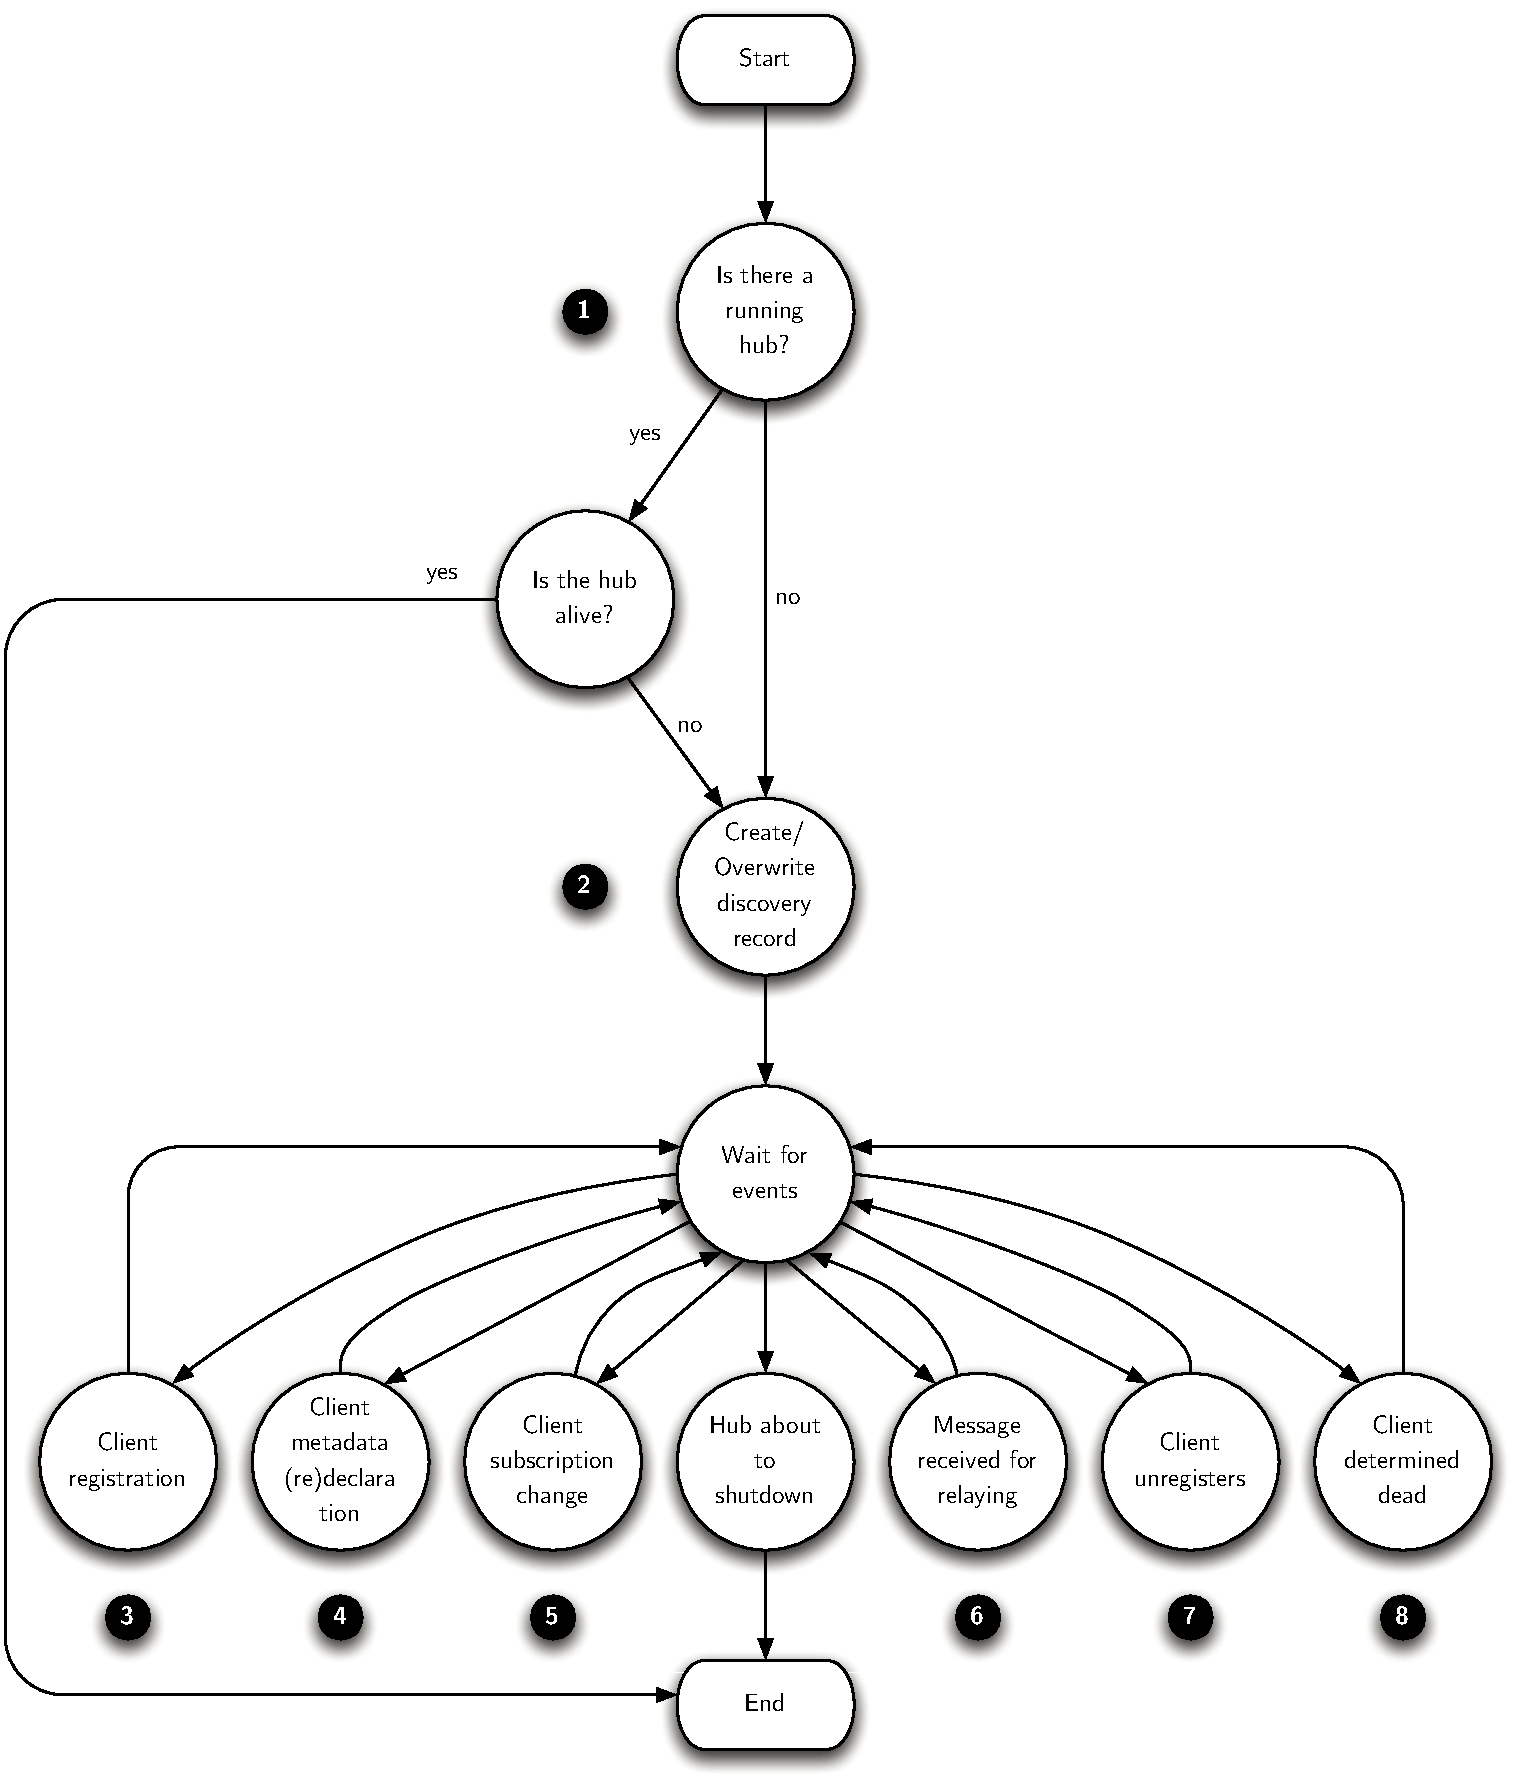
\includegraphics[width=\textwidth]
				{fig/SAMPHubLifeCycle.pdf}
				%{fig/SAMPHubLifeCycle.png}
			\caption[Life-cycle of a SAMP hub]
			{
				Life-cycle of a SAMP hub. Once determined there
				is no running, alive hub, the discovery record
				is created, and the hub waits for the different
				events it supports, until shutdown. The numbers
				on the black circles will be used to refer to
				particular steps throughout the text.
			}
			\label{fig:fig_SAMPHubLifeCycle}
		\end{figure}
		
		\begin{figure}[tbp]
			\centering
				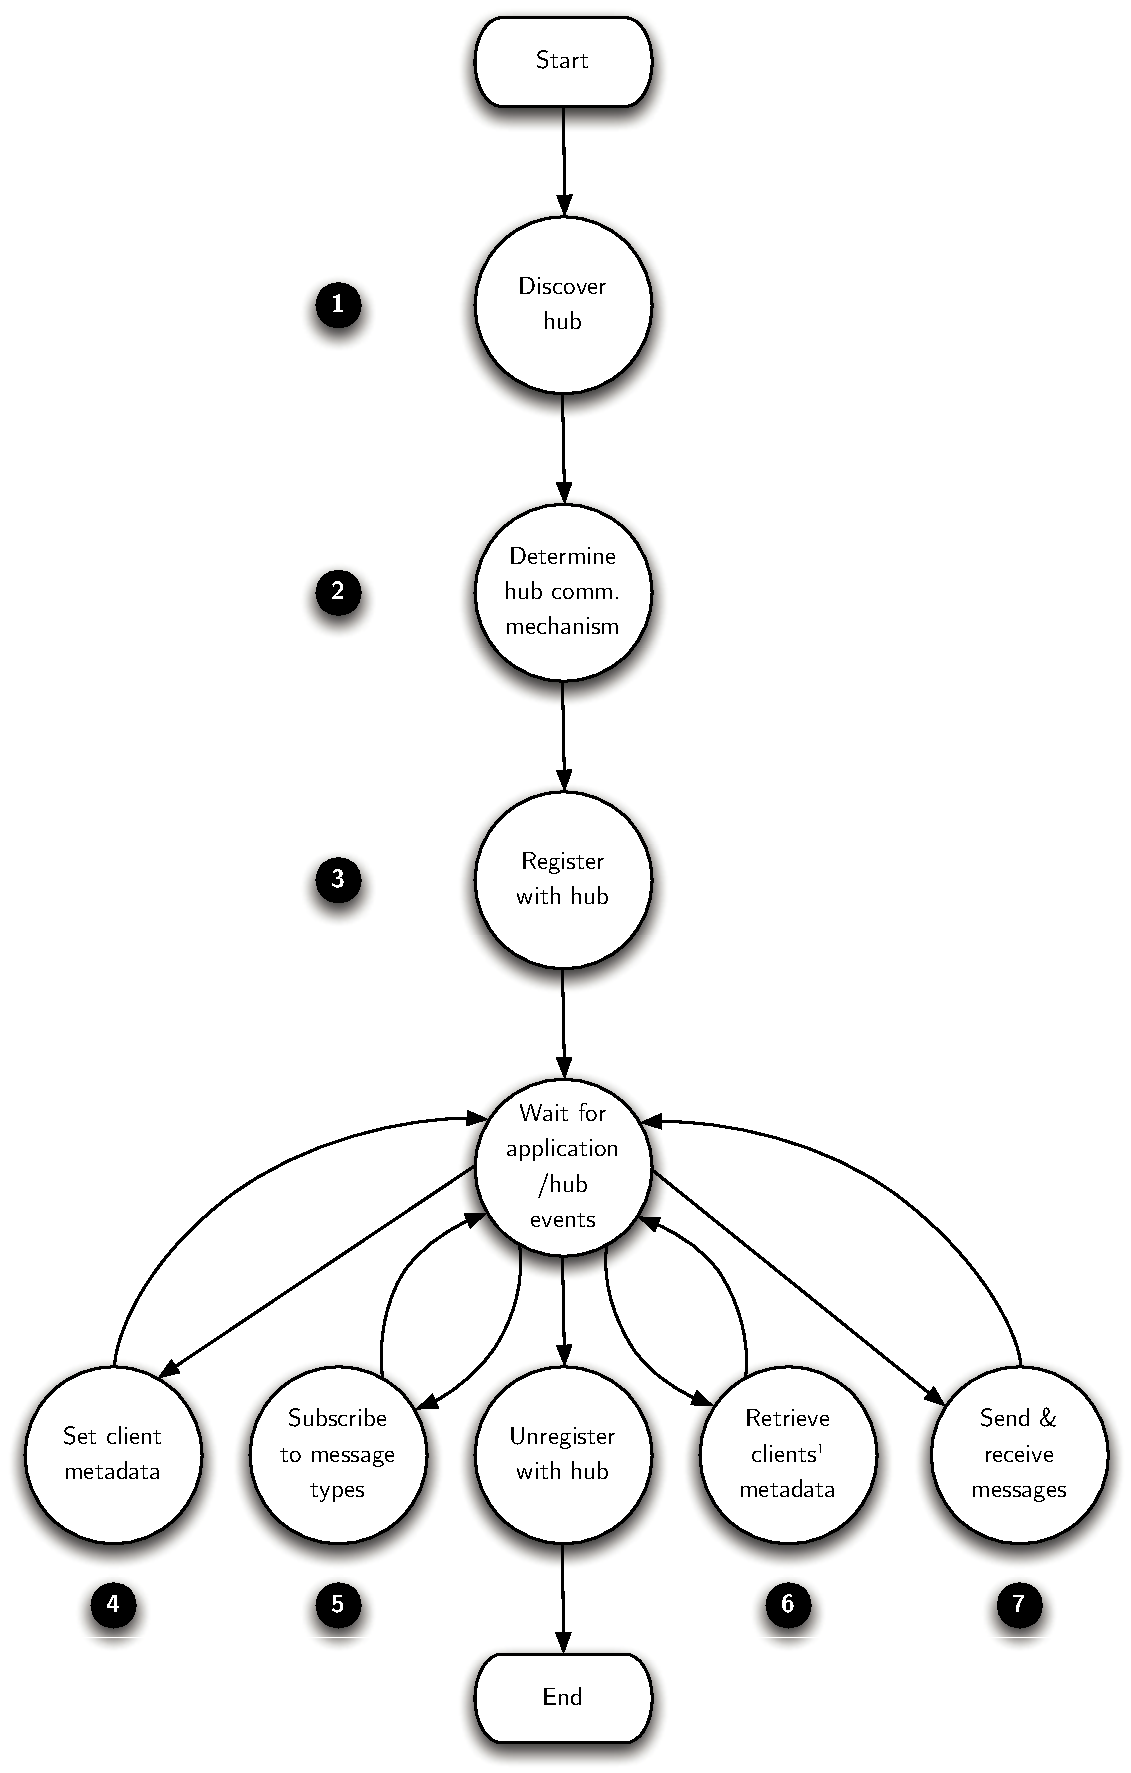
\includegraphics[width=0.75\textwidth]
				{fig/SAMPClientLifeCycle.pdf}
				%{fig/SAMPClientLifeCycle.png}
			\caption[Life-cycle of a SAMP client]
			{
				Life-cycle of a SAMP client. Once a client has
				found a hub, it registers with it, and at any
				time after registration it declares (or changes)
				metadata, subscriptions, and receives messages
				based on its subscriptions, until it unregisters
				with the hub before quitting. The numbers
				on the black circles will be used to refer to
				particular steps throughout the text.
			}
			\label{fig:fig_SAMPClientLifeCycle}
		\end{figure}
		
		
		As its predecessor, PLASTIC, SAMP is a hub-based messaging
		system, by which a intercommunication hub has to be started
		before any clients can start sending or receiving messages.
		Once the hub is started, it waits for client events, until
		shutdown condition is reached.
		
		Figure~\ref{fig:fig_SAMPHubLifeCycle} shows the complete
		life-cycle for a SAMP hub. First, the hub determines if
		there is no running, alive hub, before writing (or 
		overwriting) a new SAMP hub discovery record.
		This discovery record depends on the actual profile (or
		profiles) supported by the hub\footnote{For the standard
		profile, the hub discovery record is a file
		called \texttt{.samp}, in key=value format, stating
		the XML-RPC endpoint of the hub, among other properties.}.
		
		Once the stage has been set up, the hub waits for
		events from the clients. Supported operations are client
		registering (which gives each client a unique id for
		communication, and identification of subsequent calls),
		metadata declaration (as many times as each client
		wishes), subscription to particular message types, message
		relaying to one, several, or all clients, et cetera.
		All exchanges between SAMP applications are mediated by the
		hub, including synchronous calls between SAMP applications.
		
		Finally, when the hub is about to close, notifies all
		clients of that condition, and finally removes the
		hub discovery record, so that a new hub instance can start
		afresh.
		
		Figure~\ref{fig:fig_SAMPClientLifeCycle}, on the other hand,
		reflects the life-cycle of each SAMP client. If a hub is
		discovered\footnote{For instance, in the standard profile,
		by finding a \texttt{.samp} file at the user's home
		directory.}, it immediately enters the registration stage,
		and receives a unique identifier which allows its
		identification\footnote{Apart from that unique identifier,
		different profiles might choose additional measures in
		order to ensure there is no client spoofing. In the
		standard profile, a private key is generated by the hub
		and sent back to the client upon registration.} for
		subsequent messages. For instance, other applications might
		wish to send individual messages to applications with
		certain declared capabilities.
		
		The main difference with PLASTIC is at the message definition
		and subscription level: in SAMP, MTypes can be arbitrarily
		defined between the applications which understand them, and
		other applications can be connected to the hub without
		support for any messages other than those mandatory by the
		SAMP protocol.
		
		As the application has declared which messages does it
		subscribe to, and the function which will deal with them,
		it will only receive messages it can handle. And before
		the application is ready to quit, it should unregister
		with the hub. All application quitting events should
		handle this unregistering process, in order not to leave
		fake registered applications with the hub.
		
		Given that MTypes can be arbitrarily defined, and semantics
		and parameters are bound together by agreement between VO 
		developers within the IVOA (for public MTypes), or between
		application modules (for private MTypes), SAMP can also 
		be understood as a form of type-based publish/subscribe
		system~\cite{857078}.
		
		\invisiblenote
		{As we wish to build our system on top of the SAMP protocol,
		we need to provide a brief introduction to it.
		
		Once you have applications which are able to read and
		write both FITS files and VOTables, and which have enough
		understanding of associated metadata as to
		interoperate with VO services\footnote{That is, applications
		comply with VO data models.}, they should be able to
		consume data coming from applications in the same
		computer.
		
		An initial approach
		\begin{description}
			\item[Filesystem-based sharing] One application writes a
			file, the other application opens it. This is the
			traditional way of sharing information between
			applications. However, there is no way to bring
			attention to specific parts of the dataset, and no
			way to link actions between the two applications.
			%Some operating systems, or frameworks, such as
			%Microsoft's Object Linking and Embedding (OLE),
			%or the classic Mac OS 7 to 9 
			
			\item[Publish and Subscribe system] 
			operating systems and fram
		\end{description}}
		
		\invisiblenote{
		\todo{Speak about PLASTIC~\cite{2006pldaivoanv0606B},
		and perhaps about XPA: 
		<http://hea-www.harvard.edu/RD/PostScript/ora.ps>,
		<ftp://sao-ftp.harvard.edu/pub/rd/xpa/xpa.pdf>,
		<http://hea-www.harvard.edu/RD/xpa/>}}
		
	% section samp_messaging (end)
	
	\section{Implementing SAMP into an existing application} % (fold)
	\label{sec:implementing_samp_into_an_existing_application}
		
		We will assume the application we wish to make compatible
		with SAMP follows the Model-View-Controller (MVC) design
		pattern, because that is normally the case for GUI
		applications, and it allows for an easier discussion of
		the modifications needed.
		
		\begin{figure}[tbp]
			\centering
				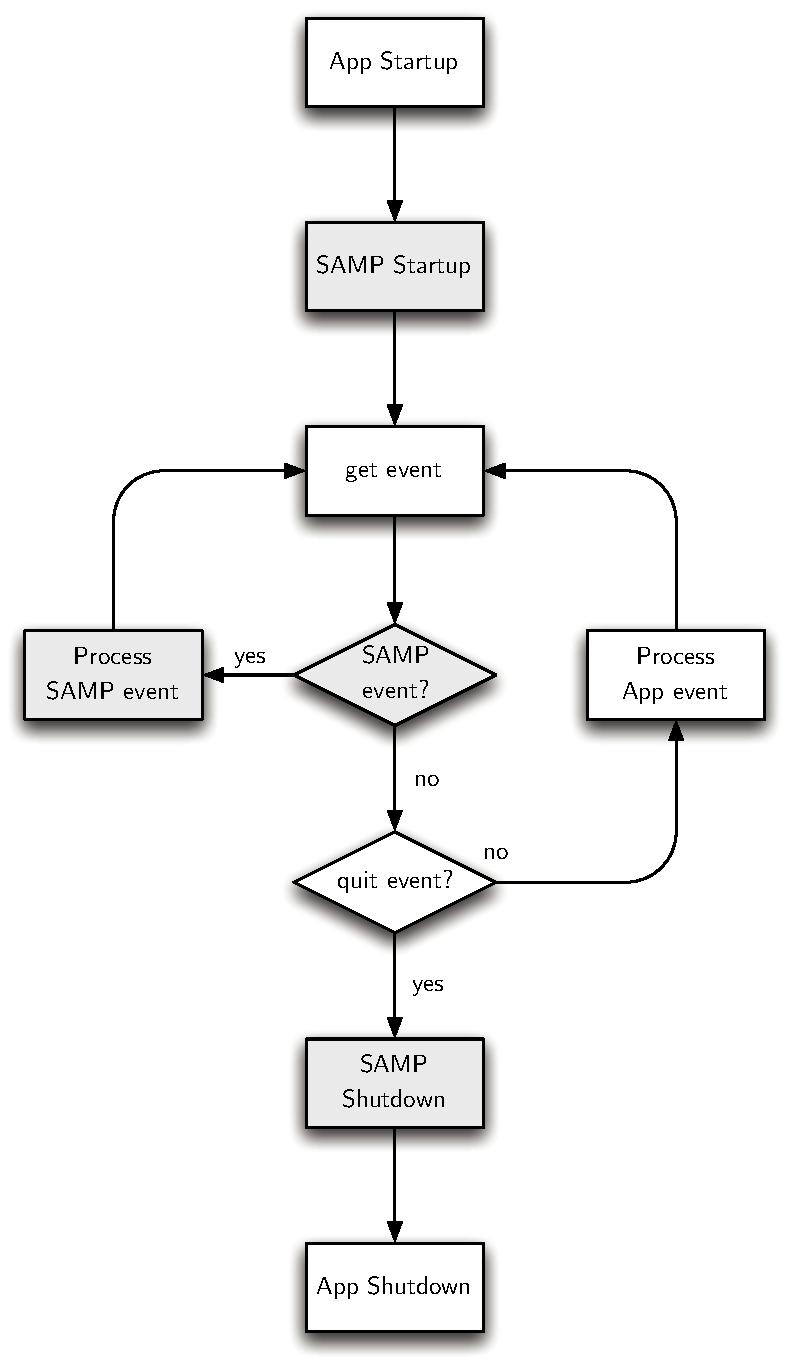
\includegraphics[height=0.6\textheight]
				{fig/SAMPEnabledAppFlow.pdf}
				%{fig/SAMPEnabledAppFlow.png}
			\caption[Simplified event flow of a SAMP-enabled
			application]
			{
				Simplified event flow of a SAMP-enabled application.
				In gray, the modules that have been introduced in
				order to provide SAMP-compatibility to an existing
				application.
				After the application has performed its start-up,
				but before entering the event-loop, we perform
				the setup of the SAMP infrastructure. We intercept
				SAMP events, in order to process them, letting the
				normal event-handling processing the rest.
			}
			\label{fig:fig_SAMPEnabledAppFlow}
		\end{figure}
		
		As the application will become a SAMP client, we need
		to add the following modules:
		
		\begin{description}
			\item[SAMP Registration module] This module would be
			added to the start-up code of the application, and
			would perform the discovery of the hub, the
			determination of the communication mechanism (in fact,
			testing that the hub corresponds to the same profile
			as the client; as we will use XML-RPC for
			communications, check the hub corresponds to the
			standard profile), and
			the registration with the hub 
			(steps 1, 2 and
			3 in figure~\ref{fig:fig_SAMPClientLifeCycle}).
			In addition, in this phase we can perform an initial
			declaration of the client metadata (step 4), and of
			the messages it subscribes to (step 5).
			
			\item[SAMP Message sending] Depending on the
			application capabilities, only a subset of possible
			MTypes will be sent. We need to create UI elements
			(buttons, pop-up menus) which provide the user with
			the possibility of sending data to other applications.
			Those pop-ups will only show applications accepting
			the messages we intend to deliver, and for that we
			will query the hub for clients' metadata (step 6).
			
			\item[SAMP Message handling] We need to implement
			the handlers for the messages we are subscribed to.
			For similitude with PLASTIC, and for extra modularity,
			a message dispatching object needs to be implemented,
			which will handle registered MTypes, which then
			dispatches the actual message to the corresponding
			handler, which in turn will make use of existing 
			application functionality to either display or
			manipulate the received message. This corresponds to
			handling of step 7.
		\end{description}
		
		In addition, some small modifications to the main view
		Controller will have to performed, so that incoming
		messages with data can be dealt with as if an \emph{open
		file} event had been issued. If the application is
		well factored, changes to the controller can be inexistent.
		
		The changes needed to the application flow are shown in 
		figure~\ref{fig:fig_SAMPEnabledAppFlow}. The main
		simplification is the \textbf{Process SAMP event} box,
		which apart from possibly reissuing application-specific
		events in order to complete event processing (i.e., for
		finishing a \emph{table load} message with an actual
		data load, in the internal data format of the application;
		if the application load messages handle FITS files, the
		changes would be minor).
		
	% section implementing_samp_into_an_existing_application (end)
	
	\section{Benefits of a SAMP-based API} % (fold)
	\label{sec:added_benefits_of_a_samp_based_environment}
		
		By implementing SAMP on an existing astronomical
		application, we have given it the opportunity to
		interact with other VO applications, and leave
		data selection in the VO to external applications.
		
		\invisiblenote
		{The main benefit from using SAMP is that we get
		modularity and messaging at the same time: there is
		less need to develop application-specific code, and
		more opportunities for code reuse.}
		
		However, given that SAMP, as a publish, subscribe, and
		messaging facility allows any kind of messages,
		by defining ad-hoc MTypes we can create new
		functionality that responds in particular ways to
		given MTypes and their parameters. This way, we can
		create a complete Application Programming Interface,
		in which instead of providing actual, byte-compiled
		functions, the functionality is provided via
		SAMP messages calls and responses.
		
		Of course, given that the standard profile for SAMP
		uses XML-RPC, we could have created such an API
		as XML-RPC instances. However, bringing the API to
		SAMP has the following advantages, both over an XML-RPC
		API or pure binary API:
		
		\begin{description}
			\item[System decoupling] By building a complete
			publish/subscribe system, we gain a three-way decoupling
			of system components~\cite{857078}:
			\begin{description}
				\item[Spatial decoupling] The \emph{spatial} term
				refers to the fact that neither publishers nor
				subscribers need to share any kind of space, or
				shared knowledge. Publishers only need to know how
				to publish, and subscribers how to subscribe to
				events.
				
				\item[Temporal decoupling] Publishers and
				subscribers do not need to orchestrate their
				interaction, and publishing is independent of
				the delivery of events to subscribers, and the
				receipt of an event to a subscribers does not need
				any interaction with the publisher.
				
				\item[Synchronism decoupling] In a true
				publish/subscribe system, such as that provided by
				SAMP, publishers are not blocked while producing
				events, and subscribers can obtain asynchronous
				notifications (via callbacks) of events: neither
				production nor consumption of messages happen in
				the main flow of control of the publishers and
				subscribers, and do not therefore happen
				synchronously.
			\end{description}
			
			\item[Modularity] The building blocks for a
			SAMP-based API are the supported MTypes, or
			families of closely related MTypes. But in any case,
			any module can provide support for one or more MTypes.
			It brings the classical \emph{do one thing well}
			motto typical from UNIX tools to the
			VO\footnote{When PLASTIC was announced, it was
			\emph{marketed} in similar terms, but many of the
			shortcomings of PLASTIC did not allow for a radical,
			modular development.}.
			
			\item[Service discoverability] In order to be
			able to receive the MType messages which conform the
			API, functional modules need to register with the
			SAMP hub. Any application can query the hub, and
			request a list of the applications (modules) which
			support particular messages. 
			\invisiblenote{The descriptions should be able to
			contain several keywords, perhaps from a UCD-like
			vocabulary, which }
			
			\item[Available for all SAMP applications] By being
			based on SAMP, a standard that many VO applications
			will implement, and thanks to the discoverability of
			SAMP-based services, we are in fact able to create a
			plug-in API for all SAMP-enabled, VO applications.
			
			\item[Easy module building] SAMP-based computing
			modules can be built in any computing language and
			operating system which provides XML-RPC support.
			In fact, as XML-RPC is an HTTP based RPC, with XML
			payloads, any language which can create sockets,
			and establish an HTTP connection, can in principle
			communicate with SAMP services\footnote{In that
			case, the most difficult part is implementing the
			callback functions.}, just by creating the XML
			as strings, and sending them over the wire in HTTP.
			This allows for SAMP module creation in the language
			the developer is more accustomed to, or having the
			best library for a particular problem.
		\end{description}
		
		The main drawback for such a message-based API when
		compared with a binary API is message latency. Function
		calls operate at the processor level (or Virtual Machine
		(VM) level, for VM-based languages such as Java, C\#, et
		cetera), while messaging needs many layers built on top of
		that.
		
		However, for interactive tasks the latency is well below
		perception limits, and is the actual computation being
		performed on the received data which will consume most of
		the time.
		
		In order to have an actual perception of the kind of
		time involved, we have used the CalcStorm testing suite
		found on the JSAMP\urlnote{\jsampurl} Java package. When
		running CalcStorm, many small clients connect to the hub,
		which understand messages for adding, subtracting,
		multiplying and dividing floating point numbers, and start
		sending calculation messages to all the rest. After
		execution, the total time elapsed is divided by the number
		of messages issued.
		
		\begin{table}[tbp]
		\begin{minipage}{\linewidth}
			\caption[JSAMP message latency tests]
			{JSAMP message latency tests. We have performed several
			timing tests with the CalcStorm testing suite of the
			JSAMP package, in a variety of situations.}
			\label{tabSAMPlatency}
		\begin{center}
		\begin{smalltabular}{cccr}
			\textbf{clients} &
			\textbf{queries} &
			\textbf{messaging kind}\footnote{\emph{sync} stands for 
											synchronous calls;
											\emph{async}
											for asynchronous;
											\emph{notify}
											for asynchronous
											notifications, without
											callbacks; and
											\emph{random} indicates
											all message kinds above
											were issued at random.}&
			\textbf{time per message} \\ \midrule
			20 & 50 & random & $10.2\pm0.3~\textrm{ms}$ \\
			\addlinespace 20 & 50 & random &
			$14.4\pm0.2~\textrm{ms}$\footnote{This result was obtained
			with an extra load on the hub caused by an additional
			testing procedure.} \\ \addlinespace 50 & 20 & notify &
			$10.7\pm0.2~\textrm{ms}$\\ \addlinespace 25 & 40 & random &
			$12.0\pm0.3~\textrm{ms}$\\ \addlinespace 1 & 1000 & random
			& $10.8\pm0.4~\textrm{ms}$\\ \addlinespace 1 & 2000 & sync
			& $10.3\pm0.3~\textrm{ms}$\\ \addlinespace 1 & 2000 & async
			& $12.6\pm0.6~\textrm{ms}$\\ \addlinespace 1 & 2000 &
			notify & $7.9\pm0.3~\textrm{ms}$\\ \addlinespace
		\end{smalltabular}
		\end{center}
		\end{minipage}
		\end{table}
		
		The results are shown on table~\ref{tabSAMPlatency},
		and where obtained on an Intel Core 2 Duo machine at
		2.4GHz, running Mac OS X 10.5.6 and a Java 1.6.0\_07 64-bit
		VM. We can see that in all cases messaging delivers
		performance which is perfectly in line with interactive
		needs: even in the slowest case, more than 68 messages per
		second could be sent and received; for computations taking
		less than messaging time to complete, real time updates can
		be provided more than 30 times per second\footnote{For
		comparison, PAL refresh rate is 25 frames per second, and
		NTSC refresh rate is 30 frames per second, which allow for
		perfectly smooth animation.}. In the best case, more than
		130 notifications per second can be delivered.
		
		We can see two additional things: First, the average cost
		for asynchronous messaging, where the calling application
		does not syncs to the response, is just 22\% higher than
		for synchronous communications. Clearly, for non-immediate
		results asynchronous messaging is the preferred, more
		robust solution, but for fast enough calculations
		synchronous messaging works better.
		
		Second, as the notify test just provides a message,
		without waiting for computation results, it can be shown
		that messaging overhead for this very simple computations
		is around 77\%. This includes the creation of the message,
		parsing of the arguments, and return of the message in XML
		format. For heavier computations, the corresponding
		messaging overhead would strongly decrease.
		
		\invisiblenote{
		 we
		obtained a figure of \invisiblenote{10687,9968,10041µs}
		$10.2\pm0.3~\textrm{ms}/\textrm{message}$ under a
		medium-load status (generated by the CalcStorm test
		itself\footnote{CalcStorm, by default, generates 20
		Calculator services which perform 100 calls between each of
		them, choosing at random between synchronous and
		asynchronous messages, and pure notifications.}), and
		\invisiblenote{14220,14517,14540µs}
		$14.40\pm0.16~\textrm{ms}/\textrm{message}$ under a
		medium-to-high-load status\footnote{Simulated by
		running simultaneously a JSAMP HubTester instance,
		another JSAMP hub testing tool.}.}
		
		We have to take into account that CalcStorm timing takes
		into account the time needed to create the clients,
		register them with the hub, perform all queries, and
		unregister them. Even when that is taken into account, all
		of that can be performed in $176\pm9~\textrm{ms}$. Most of
		the time, there are additional, higher latencies, involved
		in the kind of interactivity supported by SAMP.
		
		One more thing to note: messaging is eminently parallel, a
		very desirable feature in the days of multi-core: going
		from one core to two cores\footnote{With a monitoring
		application on to see load on each CPU}, latency jumped
		from $7.56\pm0.14~\textrm{ms}$ to $13.7\pm0.4~\textrm{ms}$,
		resulting in 1.8~times slowdown, well in line with the core
		decrease. As each execution unit can reside in different
		cores, and message parameters have to be copied in order to
		create the actual XML message, and then parsed again by the
		receiving end, there are far less opportunities for
		exploiting core-locality, providing many more opportunities
		for gains by parallelisation.
		
	% section added_benefits_of_a_samp_based_environment (end)
	
	\section{Conclusions} % (fold)
	\label{sec:legacy_conclusions}
		
		In this chapter, we have shown that, in order to bring
		astronomical legacy application into the VO one of the
		less intrusive techniques is building VO-compatible
		messaging in them, and let other applications and modules
		perform the actual interfacing with the VO.
		
		That results in a faster adaptation of legacy applications
		to the VO environment, and in a much more modular, and
		more parallel, development of VO functionality.
		
		However, in order to actually bring applications into the
		VO we need the following items to exist:
		
		\begin{description}
			\item[VO Downloader] Or file consolidator. As mentioned
			ealier, all legacy astronomical packages are able to
			read and/or write FITS files. Being able to retrieve
			both FITS files, and VOTables for later conversion, are
			the bare minimum for compatibility with the VO.
			
			\item[VO Registry and DAL module] For applications which
			have been enhanced with SAMP messaging, but have not
			implemented queries to the VO, a GUI providing access
			to data services in the VO is the way to access to
			VO data. In this module data sources will be selected,
			and once queried on a single or multiple cones, the
			data provided will be sent by SAMP messaging to
			accepting parties.
			
			\item[VOTable to FITS converter] Similar to the
			VODownloader, a VOTable to FITS converter is needed
			for providing VO compatibility with applications which
			cannot be modified.
			
			\item[Additional API] The modules above conform the bare
			minimum to provide VO compatibility for GUI, SAMP based
			applications. However, as we can provide units which
			perform arbitrary computations on the parameters
			provided (asynchronous messaging supports long execution
			times, and the called module could issue a different
			message to the calling application, depending on the
			semantics of the message sent), we can built arbitrary
			modules.
			
			In this thesis, we will demonstrate support for the
			following modules:
			
			\begin{description}
				\item[Name to coordinates resolver] Sesame is a
				web-service hosted by the CDS which provides
				coordinates for galactic and extragalactic objects,
				based on the name of the object. We will provide a
				module which will understand a series of object
				solving messages, and will deliver different kinds
				of answers.
				
				\item[FFT module] An FFT module will be developed,
				which uses both custom MTypes, but also
				\method{table.load.*} and \method{image.load.fits}
				messages, and sends back the result as
				corresponding table or image load messages to the
				calling application, so that arbitrary SAMP
				applications can make use of this computation
				facility.
			\end{description}
			
			We will provide a Python wrapper to call these
			modules from Python source code, and some of the
			modules will be written in Python as well. However,
			as the API is based on SAMP messages, any language can
			be used to write the modules, and the modules can be
			run simultaneously or one by one, as only the modules
			supporting the messages and computations we are 
			interested in need to be  \invisible{running and}
			registered with the hub.
		\end{description}
		
		In the following chapter, we will define the actual API,
		and the implementation, for the modules established above.
		
	% section legacy_conclusions (end)
	
	%As we have reiterated throughout this thesis, astrophysics is the
	%science of carefully treating received light in order to infer
	%physical properties from observed objects.
	%
	%We learn the
	%information embedded in that light by measuring the effects of
	%light on detectors, and careful processing of the light, then,
	%means we must take into account the effects of absence of
	%light on detectors, and the effects of exposing detectors with 
	%a uniform light source. Then a calibration of electron counts or 
	%voltage levels, depending on the kind of detectors, has to be 
	%performed in order to correlate that signal with the actual
	%photon flux in the received band.
	%
	%All mentioned tasks are typically performed by astronomical data
	%reduction packages, and those are just for getting a
	%correspondence between sensor output and emitted flux. After
	%that, high level analysis packages can derive 2D or 3D
	%kinematics from the data being provided.
	%
	%As a result, there is a very large number of astrophysical
	%software packages which have been developed throughout
	%the years, both for use for data from a few telescopes, or
	%for data coming from a whole family of instruments, with
	%different algorithms for data processing which might be
	%simple in some cases, or quite sophisticated in another, but
	%rely on astronomical and physical assumptions which
	%have to be kept during the processing\footnote{This is
	%particularly true for packages which rely on models of the
	%physical process, using inversion mechanisms for fitting a
	%multidimensional function from the space of parameters we wish
	%to obtain into the space of measurable properties.}.
	%
	%Once a package and/or algorithm has been debugged and
	%established, it can
	%keep being used for decades\footnote{Examples abound: AIPS 
	%<\url{http://www.aips.nrao.edu/}>
	%is a
	%radio astronomical imaging package from the late seventies 
	%originally written in FORTRAN IV,
	%while IRAF <\url{http://iraf.noao.edu/}> is an optical data 
	%reduction package from the middle
	%eighties, and GIPSY <\url{http://www.astro.rug.nl/~gipsy/}>
	%is a 3D data kinematics analysis package
	%from the early seventies, also written in FORTRAN.}.
	%That allows for easy comparison
	%of results from different teams using the same implementation,
	%and creates a barrier for changing underlying technologies.
	%
	%Indeed, 
	%re-implementing an algorithm in a new language or technology
	%is error-prone. And legacy applications in astronomy keep not
	%only their algorithms intact, but their user interfaces. This
	%makes it difficult for an emerging standard such as the
	%Virtual Observatory to be implemented 
	%
	%many man-years have been invested in
	%updating the astronomical knowledge embedded in their operation.
	%Trying to recreate such tools in more modern languages
	%(languages capable of operating with the Internet, for example)
	%would result in the introduction of calculation bugs, and the
	%investment of a lot of testing time in the ported applications.
	
%	\section{Development considerations} % (fold)
%	\label{sec:development_considerations}
%	
%		Not all legacy applications are equal from the point of
%		view of the ease of their porting to the VO.
%
%		A first classification can be made on the availability of
%		source code for the application (or a contact with the
%		application maintainer), and latter on the capabilities of
%		the programming language the application has been written
%		in:
%	
%		\begin{enumerate}
%			\item Applications without available source code nor
%			maintainer.
%		
%			\begin{enumerate}
%				\item Applications with an RPC interface or public
%				API.
%				
%				 \item Applications without an RPC or public API.
%			\end{enumerate}
%	
%			\item Applications with available source code (or
%			maintainer)
%	
%			\begin{enumerate}
%				\item Applications written in Internet and XML-aware
%				languages.
%				
%				 \item Applications written in non-Internet or
%				XML-aware languages.
%			\end{enumerate}
%		\end{enumerate}
%	
%		This classification affects the different courses of action
%		we can take for making the legacy application VO-compatible:
%	
%		\begin{enumerate}
%			\item Application source code is not available, and no
%			contact is possible with the original application
%			developer:
%	
%			\begin{enumerate}
%				\item If the application does not have an RPC
%				interface, nor a public API, the only possible
%				course of action is having an external VO data
%				downloader, and rely on the compatibility with
%				either FITS files, or with tabular data formats such
%				as CSV, TST, et cetera. Interoperation with other VO
%				tools is only possible by importing products in the
%				most suitable tool. This is the case for many
%				applications.
%				
%				 \item If the application provides a public RPC
%				interface, or API, building a module that translates
%				external petitions into the application is feasible,
%				depending on the published interfaces. All of the
%				data transformation into the application specific
%				data models and data formats must be performed
%				outside of the application.
%				
%				 In this case we have two sub-cases:
%				
%				\begin{enumerate}
%					\item The RPC interfaces/API allow for callback
%					methods. This is the best case for applications
%					for which it is not possible to get access to
%					the source code. An intermediate VO module can
%					send data to the legacy application, but can
%					also register callback methods to be called when
%					the legacy application wants to send data back.
%					
%					\item RPC interfaces/API do not allow for
%					callback methods. In this case, the intermediate
%					VO module can send data to the legacy
%					application, but the application cannot interact
%					with the VO.
%				\end{enumerate}
%				
%			\end{enumerate}
%	
%			\item Application source code is available (or the
%			maintainer wishes to bring his tool into the Virtual
%			Observatory).
%			
%			The corresponding two sub-cases depend on the programming
%			language capabilities:
%			
%			\begin{enumerate}
%				\item If the programming language has libraries to
%				interact with the Internet, and to manipulate XML
%				and FITS files, we are in the best possible case, as
%				the application will not only be able to receive
%				data from the VO (via an established public API, or
%				by creating one), but also to send queries to the VO
%				and retrieve data (creating the appropriate query
%				methods). We will use this approach for applications
%				based on Java or modern, internet-aware scripting
%				languages such as Python.
%				
%				 \item If the programming language lacks libraries
%				to interact with the Internet, or for manipulating
%				XML and FITS files, those will have to be built
%				first, or rely on a VO downloader as in the \emph{no
%				source code} case.
%			\end{enumerate}
%	
%		\end{enumerate}
%		
%	
% section development_considerations (end)
	
%	\section{Decisions} % (fold)
%	\label{sec:decisions}
%		
%		In this thesis, we have created a modular VO tool which
%		decouples VO interaction from the adaptation of the VO
%		data model to the internal application data model.
%	
%		With this approach, three modules are needed:
%	
%		\begin{itemize}
%
%			\item a VO interaction module is created, with an
%			emphasis on radio astronomical data and in both GUI and
%			scripting operation, which can be used either
%			standalone or for providing legacy (or new) applications
%			with VO services;
%		
%			 \item an application-specific module, either built
%			inside the application source code, or calling the
%			application API or callbacks, which communicates with
%			the VO interaction module for VO services.
%		
%			 \item and several helper modules: a generic VO Downloader
%			which can be used for applications for which the only VO
%			compatibility is the FITS file; a VO Data Access and Query
%			module; which is used to retrieve the data for all other
%			modules; and a sample calculation module, which can
%			provide advanced calculation services to VO applications,
%			but also to any application able to call XML-RPC services.
%
%		\end{itemize}
%		
%		We will describe those modules in the next chapter, 
%		together with the VO Downloader, and we will
%		describe how to create the application-specific module for
%		a particular application, the \massa{} spectral analysis tool,
%		in chapter~\ref{cha:massa_and_movoir}.
	
	
	
	% In any case, the best possible outcome for bringing a legacy
	% application into the VO is being able to implement one of
	% IVOA's messaging protocols, either PLASTIC or SAMP, and
	% integrating the messaging mechanism in the controller of the

	% In the following sections, we will show two examples of
	% bringing legacy applications into the VO, one corresponding
	% to the closed-source kind, and another one corresponding to
	% an application written in Java (a programming language with
	% libraries for XML, FITS, and Internet interaction.)
	% 
	%  But first, we will analyse exactly what needs to be
	% provided for both kinds of applications, so that a common
	% strategy can be built.
	
	% section decisions (end)
	
%	\section{Common features of a VO wrapper module} % (fold)
%	\label{sec:common_features_of_a_vo_wrapper_module}
%	
%	% section common_features_of_a_vo_wrapper_module (end)
	
%	\section{An example: \massa{}} % (fold)
%	\label{sec:an_example_massa}
%	
%	\subsection{What is \massa{}?} % (fold)
%	\label{sub:what_is_massa}
%	
%	% subsection what_is_massa_ (end)
%	
%	\subsection{Internal \massa{} data model} % (fold)
%	\label{sub:internal_massa_data_model}
%	
%	% subsection internal_massa_data_model (end)
%	
%	\subsection{Coupling \massa{} with PLASTIC/SAMP} % (fold)
%	\label{sub:coupling_massa_with_plastic_samp}
%	
%	% subsection coupling_massa_with_plastic_samp (end)
%	
%	
%	% section an_example_massa (end)
%	
%	\section{Another example: \textsc{GIPSY}} % (fold)
%	\label{sec:another_example_gipsy}
%	
%		The \emph{Groningen Image Processing
%		SYstem}~\cite{1980tdp..conf..169S, 1985daa..conf..271A,
%		1992ASPC...25..131V, Terlouw:1992lq} (GIPSY) is a software
%		package developed in the seventies at the Kapteyn Institute
%		of Groningen for scientifically treating the data cubes of
%		the Westerbork Synthesis Radio Telescope (WRST) in order to
%		extract physical parameters (rotation curves, warped or
%		non-warped disc models, velocity fields...) by fitting
%		spectral lines to emission intensity, calculating relative
%		speeds in observed galaxy reference frame, and then fitting
%		a disc and a bulge distribution.
%		
%		 The core GIPSY system was originally written in C, while
%		many processing routines where written in FORTRAN, as many
%		scientific processing applications of the time. GIPSY
%		contains many algorithms which are really useful for the
%		scientific exploitation of radio astronomical data cubes,
%		such as:
%		
%		 All of these tools share a common data model ---see section
%		on the GIPSY data structure (GDS)
%		in~\cite{1992ASPC...25..131V}--- for the data cubes they can
%		work with, which allows slicing the cube in one or more
%		dimensions, and with variable sizes, so that slices
%		consisting of single planes, single rows, or even single
%		pixels, in any dimension, can be tagged with custom
%		metadata. All of this different slices are kept together in
%		the same file, and the different subsets and tags are kept
%		separate of the data.
%		
%		 GIPSY has a scripting language, COLA (\emph{COntrol
%		LAnguage}), that allows both interactive and non-interactive
%		scripts to have access to the GDS, and either call existing
%		GIPSY tasks with parameters fixed in the script, retrieving
%		results, or perform calculations on their own.
%		
%		 In recent times, GIPSY has been enhanced with Python
%		bindings for COLA, something that allows using GIPSY
%		routines, and GDS access, within the Python environment, and
%		to import Python packages from the COLA environment. As we
%		can see from our discussion on the properties of legacy
%		packages, this opens the door of the VO for GIPSY, as Python
%		is an Internet and Web services aware language, for which
%		many VO tools exist.
%		
%		 \todo{Check assertion before.}
%			
%			 The planned strategy for updating GIPSY and incorporating
%            VO capabilities is the following:
%	
%		\begin{enumerate}
%			\item Complete GIPSY Python bindings, so that both
%			Python scripts can use GIPSY facilities, and COLA
%			scripts can make use of Python modules.
%			
%			 \item Rewrite most existing COLA scripts as Python
%			modules. Modules rewritten in Python will automatically
%			earn 64-bit cleanness, and
%			
%			 \item Create Python scripts to perform the following VO
%			functions:
%			
%			\begin{itemize}
%				\item Perform ConeSearch queries on the region of
%				the sky being viewed, or any other the script might
%				ask for.
%				
%				 \item Send PLASTIC and/or SAMP messages to other
%				applications with the content of image planes or
%				spectra.
%				
%				 \item Enhance GIPSY controller to be PLASTIC and/or
%				SAMP aware, so that it can receive data coming from
%				other VO applications.
%			\end{itemize}
%		\end{enumerate}
%	
%		As there is no IVOA recommended data model for cubes, we
%		will try to standardise a data format that is compatible
%		with ALMA and existing tools. There is some work already
%		performed for standardising IFUs 3D spectra, such as the
%		Euro3D data format \cite{2004AN....325..159K}.
%		
%		 This author has entered the IVOA Data Modelling Working
%		Group with the aim of contributing both with the RADAMS, and
%		with a future 3D metadadata standard for 3D datasets within
%		the VO.
%	
%	
%	% section another_example_gipsy (end)
%	
%	\section{Conclusions} % (fold)
%	\label{sec:legacy_conclusions}
%	
%	 - For legacy apps, th
%	
%	% section legacy_conclusions (end)

% chapter using_legacy_tools (end)

	% chapter movoir (fold)
\chapter[MOVOIR: MOdular VO InteRface]
		[The MOVOIR]
		{MOVOIR:
         MOdular Virtual Observatory InteRface, and VO APIs}
\label{cha:movoir}

	\attributedquote{
		\dictionarydef
		{modular}
		{adjective}
		{
			\begin{itemize}
				\item employing or involving a module or modules
				as the basis of design or construction.
				\invisiblenote{: \emph{modular housing units}.} 
			\end{itemize}
		}
		\dictionarydef
		{module}
		{noun}
		{
			\begin{itemize}
				\item each of a set of standardized parts or 
				independent units that can be used to 
				construct a more complex structure.
				
				\item \textsf{Computing} any of a number of distinct
				but interrelated units from which a 
				program may be built up or into which a complex 
				activity may be analyzed.
			\end{itemize}
		}
		\dictionarydef
		{interface}
		{noun}
		{
			%\begin{enumerate}
			%	\item
				\begin{itemize}
					\item a point where two systems, subjects,
					organizations, etc., meet and interact.
					\invisiblenote{:
					\emph{the interface between accountancy
					and the law}.}
					
					\invisiblenote
					{\item \textsf{chiefly Physics} a surface
					forming a common boundary between two portions
					of matter or space, e.g., between two
					immiscible liquids:
					\emph{the surface tension of a liquid at 
					its air/liquid interface}.} 
			%	\end{itemize}
				
			%	\item 
			%	\begin{itemize}
					\invisiblenote{
					\item a device or program
					enabling a user to communicate with a computer.}
					
					\item \textsf{Computing}
					a device or program for connecting two
					items of hardware or software so that 
					they can be operated jointly or communicate
					with each other.
				\end{itemize} 
			%\end{enumerate}
		}
	}
	{The New American English Dictionary, \emph{2nd Edition}}
	
	\invisiblenote{
	The MOVOIR (acronym for MOdular Virtual Observatory InteRface)
	}
	
	In the previous chapter we have seen that by creating
	applications which support VO messaging, using the SAMP
	messaging protocol, the application can be completely
	VO-enabled as long as there are outside modules performing
	certain functions.
	
	 In this chapter, we will show a set of such modules, which we
	call MOVOIR (as acronym for MOdular Virtual Observatory
	InteRface). We will see which are the messages used by already
	existing applications, and how can we create our own messages
	for supporting an interface to the VO, but also the messages
	defined by the existing applications can be rethought so that
	the support special services, defining that way a plug-in API
	for the VO.
	
	 An additional remark: in this, and the following chapters,
	the meaning of the words “MUST”, “MUST NOT”,
	“REQUIRED”, “SHALL”, “SHALL  NOT”, “SHOULD”, “SHOULD NOT”,
	“RECOMMENDED”, “MAY”, and “OPTIONAL”, when they appear in
	capital letters, are to be interpreted as described by
	Internet Engineering Task Force (IETF)
	RFC~2119\urlnote{http://www.ietf.org/rfc/rfc2119.txt}~\cite{
	rfc2119}.
	
	\section{SAMP Messages and MTypes} % (fold)
	\label{sec:samp_messages_mtypes}
		
		SAMP is a hub-based messaging system which supports many
		different mechanisms for messaging: message broadcasting,
		point-to-point messaging, and a publish/subscribe scheme
		where messages are sent to all interested applications,
		which have declared such interest when registering with
		the hub.
		
		All of these operations are performed by sending MTypes,
		which are messages with particular codes, so that they
		have an associated meaning. In the SAMP standard profile,
		they correspond to XML-RPC calls to the hub to the
		corresponding \method{call}, \method{callAndWait}, or
		\method{notify} methods, provided as XML-RPC services by
		the hub. In those calls, there is a message parameter
		which correspond to a map (in the sense of a set of
		key-value pairs, where the keys are strings) with the
		following keys:
		
		\begin{description}
			\item[\sampmtype] A \stringtype{} which
			defines the meaning and parameters of the message.
			All messages sent with the same \sampmtype{}
			need to provide the same mandatory parameters, with
			the same data types, with the same expected behaviour.
			
			\item[\sampparams] A \maptype{} of
			the parameters needed for the correct interpretation
			of a message with the specified \sampmtype.
			As mentioned above, when an MType is defined, their
			mandatory parameters have to be defined, too.
			Keys are \stringtype{}s representing the parameter
			name, and the data type of the value depends on the
			actual definition of the MType, but has to be one of
			the supported data types.
		\end{description}
		
		\begin{table}[t]
		\begin{minipage}{\linewidth}
			\caption[SAMP data types]
			{SAMP Data Types. The corresponding Backus-Naur Form
			(BNF)
			for each data type can be found on section 3.3 of the
			\emph{SAMP IVOA Recommendation}~\cite{2009samp.ivoav0904T}.
			Data range for \sampint{} or \sampfloat{} types depends
			on the encoding and decoding applications.}
			\label{tabSAMPdataTypes}
		\begin{center}
		\begin{smalltabular}{rp{0.5\textwidth}}
			\textbf{Data type} & \textbf{Description} \\ \midrule
		
			\stringtype{} & alphanumeric data.\\ \addlinespace
			
			\listtype{} & ordered array of data
			items of the same type.\\ \addlinespace
			
			\sampint{} & a \stringtype{} containing a
			representation of an integer number.\\ \addlinespace
			
			\sampfloat{} & a \stringtype{} containing a
			representation of a floating point number.\\
			\addlinespace
			
			\sampbool{} & a \stringtype{} containing either
			\datatype{0} or \datatype{1}, for false or true logical
			values, respectively.\\ \addlinespace
			
			\maptype{} & an unordered associative
			array of key-value pairs, in which each key is a
			\stringtype, and each value is given in one of
			the supported data types above.\\ \addlinespace
		\end{smalltabular}
		\end{center}
		\end{minipage}
		\end{table}
		
		When a message of a given type returns values, they are
		returned as map with the following keys:
		
		\begin{description}
			\item[\sampstatus] This is a REQUIRED key.
			Its value is a \stringtype{} summarising the result
			of the processing. It may take one of the following
			predefined values:
			
			\begin{description}
				\item[\sampok] Signals total
				success. In this case, the \sampresult{} key
				SHOULD be present, and the \samperror{} key
				SHOULD NOT appear.
				
				\item[\sampwarning] Partial success. Both
				\sampresult{} and \samperror{} keys
				SHOULD be present.
				
				\item[\samperror] Processing of the
				message failed. The \samperror{} key MUST
				be present, and the \sampresult{} MUST NOT
				appear.
			\end{description}
			
			\item[\sampresult] This key is REQUIRED in case
			of full (\sampstatus\ equal to \sampok) or partial
			(\sampstatus\ equal to \sampwarning) success. The
			value is a map containing the values for the
			named return values, which are determined by the
			value of \sampmtype{} (the MType). Even for MTypes
			which return no value, the key must be present,
			with its value set to empty.
			
			\item[\samperror] This key is REQUIRED in case
			of full (\sampstatus\ equal to \samperror) or
			partial (\sampstatus\ equal to \sampwarning) error.
			The value for this key is a map with the following
			keys:
			
			\begin{description}
				\item[\mapkey{samp.errortxt}] This key is
				REQUIRED in this map. Its value is short
				\stringtype{} describing the problem, to be
				presented to the user.
				
				
				\item[\mapkey{samp.usertxt}] This key is
				optional, and its value is a free-form
				\stringtype, with additional text the
				called application wishes to append to the error.
				It could be appended to the \mapkey{samp.errortxt},
				but it is undefined what to do with it.
				
				\item[\mapkey{samp.debugtxt}] This key is optional,
				and its value is a free-form \stringtype{} of interest
				for debugging purposes (e.g. a stack trace).
				
				\item[\mapkey{samp.code}] This key is optional, and
				its value is a \stringtype{} containing a code
				(numeric or textual) identifying the error.
			\end{description}
		\end{description}
		
		In order to enhance interoperability, SAMP data types
		are specified as encoded strings, instead of having
		a binary encoding, or using platform specific types such
		as native XML-RPC \mapkey{int} or \mapkey{float} types.
		Allowed data types are shown in table~\ref{tabSAMPdataTypes}.
		
	% section samp_messages_mtypes (end)
	
	\section{Standard SAMP message types (MTypes)} % (fold)
	\label{sec:already_defined_mtypes}
		
		\begin{figure}[tb]
			\centering
				\begin{minipage}{0.85\linewidth}
				\begin{framed}
					\begin{small}
						\mtypedef{String encoding an MType in
						\sampmtype}
								{
									Description of the meaning of 
									the message, including the
									expected behaviour of receiving
									applications.
								}
								{
									\mtypeparam{parameter name}
									{data type}
									{
										An entry describing every
										allowed \mapkey{parameter
										name}
										in \sampparams.
										All parameters are mandatory,
										unless otherwise stated.
									}
								}
								{
									\mtypeparam{parameter name}
									{data type}
									{
										\emph{None}, if nothing is
										returned, or one entry for
										each named
										returned parameter supported
										in \sampparams, 
										describing it.
									}
								}
					\end{small}
				\end{framed}
				\end{minipage}
				
			\caption{Format for describing MTypes.}
			\label{fig:sampMTypeDescFormat}
		\end{figure}
		
		As SAMP is an evolution of the PLASTIC messaging protocol,
		there have been defined some MTypes which represent the
		kind of messages, with their parameters, that PLASTIC
		applications were capable of sending.
		
		\newcommand{\sampmtypesurl}[0]
		{http://www.ivoa.net/cgi-bin/twiki/bin/view/IVOA/SampMTypes}
		The Applications Working Group of the IVOA has created a
		wiki page\urlnote{\sampmtypesurl} for declaring the
		MTypes being publicly supported by different applications,
		so that applications can open up for ad-hoc messages. Once
		this thesis is published, the MTypes for the MOVOIR will be
		incorporated to this page.
		
		In particular, only the following MTypes are officially
		supported by clients such as TOPCAT and Aladin, and
		maintained by the IVOA Applications WG:
		\method{ta\-ble.load.vo\-ta\-ble}, \method{ta\-ble.load.fits},
		\method{ta\-ble.high\-light.row},
		\method{ta\-ble.se\-lect.row\-List},
		\method{im\-age.load.fits},
		\method{coord.point\-At.sky}, and
		\method{spec\-trum.load. ssa-generic}. They are shown,
		following the format of
		figure~\ref{fig:sampMTypeDescFormat}, in
		figures~\ref{fig:tableLoadVotableMtype},
		\ref{fig:tableLoadFitsMtype},
		\ref{fig:tableHighlightRowMtype},
		\ref{fig:tableSelectRowListMtype},
		\ref{fig:imageLoadFitsMtype},
		\ref{fig:coordPointAtSkyMtype}, and
		\ref{fig:spectrumLoadSsaGenericMtype}.
		
		\begin{figure}[tbp]
			\centering
			\begin{minipage}{0.9\textwidth}
				\begin{framed}
					\mtypedef{table.load.votable}
							{
								Load (possibly display, or otherwise
								acknowledge the receipt of) a table in
								VOTable format.
							}
							{
								\mtypeparam{url}{string}{
									URL of the VOTable document to
									load.
								}

								\mtypeparam[optional]{table-id}{string}
								{
									Identifier which may be used to
									refer to the loaded table in
									subsequent messages.
								}

								\mtypeparam[optional]{name}{string}{
									Name which may be used to label the
									loaded table in the application
									GUI.
								}
							}
							{\mtypeparamnone}
				\end{framed}
			\end{minipage}
			
			\caption[\method{table.load.votable} MType description]
			{Description of the \method{table.load.votable} MType.}
			\label{fig:tableLoadVotableMtype}
		\end{figure}
		
		\begin{figure}[tbp]
			\centering
			\begin{minipage}{0.9\textwidth}
				\begin{framed}
					\mtypedef{table.load.fits}
							{
								Load (possibly display, or otherwise
								acknowledge the receipt of) a data
								table in FITS format.
							}
							{
								\mtypeparam{url}{string}{
									URL of the FITS file to load.
								}
							
								\mtypeparam[optional]{table-id}{string}
								{
									Identifier which may be used to
									refer to the loaded table in
									subsequent messages.
								}
							
								\mtypeparam[optional]{name}{string}
								{
									Name which may be used to label the
									loaded table in the application GUI.
								}
							}
							{\mtypeparamnone}
				\end{framed}
			\end{minipage}
			\caption[\method{table.load.fits} MType description]
			{Description of the \method{table.load.fits} MType.}
			\label{fig:tableLoadFitsMtype}
		\end{figure}
		
		\begin{figure}[tbp]
			\centering
			\begin{minipage}{0.9\textwidth}
				\begin{framed}
					\mtypedef{table.highlight.row}
							{
								Highlights a single row of an
								identified table by row index. The
								table to operate on is identified by
								one or both of the \mapkey{table-id} or
								\mapkey{url} arguments. At least one of
								these MUST be supplied; if both are
								given they should refer to the same
								thing. Exactly what highlighting means
								is left to the receiving application.
							}
							{
								\mtypeparam[optional, if \mapkey{url} is
								specified]{table-id}{string}
								{
									identifier associated with a table,
									established by a previous message
									(e.g. \mapkey{ta\-ble.load.*})
								}

								\mtypeparam[optional, if
								\mapkey{table-id} is
								specified]{url}{string}{URL of a table.}

								\mtypeparam{row}{SAMP int}
								{
									Row index (zero-based) of the row
									to highlight.
								}
							}
							{\mtypeparamnone}
				\end{framed}
			\end{minipage}
			\caption[\method{table.highlight.row} MType description]
			{Description of the \method{table.highlight.row} MType.}
			\label{fig:tableHighlightRowMtype}
		\end{figure}
		
		\begin{figure}[tbp]
			\centering
			\begin{minipage}{0.9\textwidth}
				\begin{framed}
					\mtypedef{table.select.rowList}
							{
								Selects a list of rows of an identified
								table by row index. The table to
								operate on is identified by one or both
								of the \mapkey{table-id} or
								\mapkey{url} arguments. At least one of
								these MUST be supplied; if both are
								given they SHOULD refer to the same
								thing. Exactly what selection means is
								left to the receiving application.
							}
							{
								\mtypeparam[optional, if \mapkey{url} is
								specified]{table-id}{string}
								{
									Identifier associated with a table,
									established by a previous message
									(e.g. \mapkey{ta\-ble.load.*})
								}

								\mtypeparam[optional, if
								\mapkey{table-id} is
								specified]{url}{string}{URL of a table.}

								\mtypeparam{row}{list of SAMP int}
								{
									List of row indices (zero-based)
									defining which table rows are to
									form the selection
								}
							}
							{\mtypeparamnone}
				\end{framed}
			\end{minipage}
			
			\caption[\method{table.select.rowList} MType description]
			{Description of the \method{table.select.rowList} MType.}
			\label{fig:tableSelectRowListMtype}
		\end{figure}
		
		\begin{figure}[tbp]
			\centering
			\begin{minipage}{0.9\textwidth}
				\begin{framed}
					\mtypedef{image.load.fits}
							{
								Load (possibly display, or otherwise
								acknowledge) a two-dimensional FITS
								image.
							}
							{
								\mtypeparam{url}{string}
								{URL of the FITS image to be loaded.}

								\mtypeparam[optional]{image-id}{string}
								{
									Identifier which may be used to
									refer to the loaded FITS image in
									subsequent messages.
								}

								\mtypeparam[optional]{name}{string}
								{
									Name which may be used to label the
									loaded FITS image in the
									application GUI.
								}
							}
							{\mtypeparamnone}
				\end{framed}
			\end{minipage}
			
			\caption[\method{image.load.fits} MType description]
			{Description of the \method{image.load.fits} MType.}
			\label{fig:imageLoadFitsMtype}
			
		\end{figure}
		
		\begin{figure}[tbp]
			\centering
			\begin{minipage}{0.9\textwidth}
				\begin{framed}
					\mtypedef{coord.pointAt.sky}
							{
								Directs attention (e.g. by moving a
								cursor or shifting the field of view)
								to a given point on the celestial
								sphere.
							}
							{
								\mtypeparam{ra}{SAMP float}
								{Right ascension in degrees.}

								\mtypeparam{dec}{SAMP float}
								{Declination in degrees.}
							}
							{\mtypeparamnone}
				\end{framed}
			\end{minipage}
			
			\caption[\method{coord.pointAt.sky} MType description]
			{Description of the \method{coord.pointAt.sky} MType.}
			\label{fig:coordPointAtSkyMtype}
		\end{figure}
		
		\begin{figure}[tbp]
			\centering
			\begin{minipage}{0.9\textwidth}
				\begin{framed}
					\mtypedef{spectrum.load.ssa-generic}
							{
								Load (possibly display, or otherwise
								acknowledge) a spectrum or SED. The
								name refers to the fact that the
								metadata passed with this MType is
								based on the Simple Spectral Access
								protocol, but not on any particular
								version of it. The arguments are chosen
								such that it is convenient to use this
								MType for passing the results of an SSA
								query from an SSA client to a spectrum
								viewer (particularly to an SSA-capable
								spectrum viewer). However it is not
								necessary for SSA to be involved;
								SSA-like metadata may be faked and used
								to message loading of a spectrum from
								any source. In the latter case it is
								RECOMMENDED to provide at least the
								\mapkey{Access.Format} entry in the
								\mapkey{meta} map.
							}
							{
								\mtypeparam{url}{string}
								{URL of the spectrum to load}

								\mtypeparam{meta}{map}{
									Additional metadata describing the
									spectral data found at the URL.
									Key/Value pairs represent either
									Utypes or UCDs as defined or used
									in some version of the SSA
									specification or its predecessors.
									Example map keys are
									\mapkey{Access.Format} (SSA 1.0
									MIME type Utype) or
									\mapkey{VOX:Spectrum\_Format}
									(pre-1.0 SSA MIME type UCD). It is
									up to the recipient to make sense
									of these and, for instance, deal
									with the possibility that given
									expected keys are present or that
									apparently contradictory
									information is presented. Most
									existing SSA-aware spectrum viewing
									clients already contain this
									functionality.
								}

								\mtypeparam[optional]{spectrum-id}
								{string}
								{
									Identifier which may be used to
									refer to the loaded spectrum in
									subsequent messages.
								}

								\mtypeparam[optional]{name}{string}
								{
									Name which may be used to label the
									loaded spectrum in the application
									GUI.
								}
							}
							{\mtypeparamnone}
				\end{framed}
			\end{minipage}
			
			\caption[\method{spectrum.load.ssa-generic} MType
			description]
			{Description of the \method{spectrum.load.ssa-generic}
			MType.}
			\label{fig:spectrumLoadSsaGenericMtype}
		\end{figure}
		
				
		We can see in the message descriptions that applications
		developers' flexibility is encouraged, but an additional
		property of all of these messages collaborates in that
		flexibility: none of the MTypes above return anything, and
		the actions to be carried out by the receiving  application
		upon receipt of these messages can be completely arbitrary.
		
		We will use this flexibility to define a set of
		\emph{behaviours}, upon receipt of standard MTypes, which
		will aid in calculations, and will provide the API for
		the MOVOIR operations.
		
	% section already_defined_mtypes (end)
	
	% section movoir_alternative_behaviours (fold)
	\section{Creating alternative response patterns}
	\label{sec:movoir_alternative_behaviours}
		
		We have seen in the previous section that there are a 
		number of already standardised MTypes, together with their
		corresponding responses upon receipt of those MTypes.
		For all of those messages applications returned
		nothing\footnote{Formally, asynchronously called modules
		which return nothing SHOULD call the callers' \method{reply}
		method with a \maptype\ with keys \sampstatus\ set to
		\sampok\, and \sampresult\ set to an empty map, but
		applications
		SHOULD NOT behave incorrectly if they do not receive it.},
		and there were clear indications that applications should
		perform certain tasks upon receipt of such MTypes, but
		there is nothing the caller application can do in order to
		ensure a particular response, and this is a feature of this
		messaging system: applications are notified of an event,
		and what to do upon reception is completely up to them.
		
		One clear case of SAMP-based application which subscribes
		to the messages above, but does not really perform the
		actions specified by the MType description, are logger
		application. A typical logger application would register
		with a SAMP hub, and subscribe to every possible message.
		However, for all messages received the message handler
		is the same, and just logs the \sampmtype{} and \sampparams{}
		of the call, together with information about the caller
		application.
		
		The lesson to learn from this example is that applications
		which subscribe to broadcasted messages, and specially
		those who require no answer, are completely transparent to
		caller applications: we can perform any action it makes
		sense to perform upon receipt of these messages, as long
		as the formal behaviour expected by the calling application
		(in terms of answering a synchronous message, not letting
		the calling application blocked, filling all required
		keywords in the response...) is fulfilled.
		
		Let us explore a few examples of new functionality which
		can be added by two means: performing a somewhat different
		action upon receiving one of the standard messages, or
		letting called applications see who has called them, and
		send messages back to applications which support them.
		
		\subsection{Modifying or enhancing response actions} % (fold)
		\label{sub:modifying_or_enhancing_response_actions}
			The first case (modifying what is done by the receiving
			applications) was illustrated by our previous example of
			a logger application, and we will also use this way to
			create a VODownloader application.
			
			A VODownloader is, essentially, an application which,
			instead of actually working with the VOTables and FITS
			files which are sent to it, it downloads and saves them
			to a particular folder. This requires being able to
			respond to the \mapkey{table.load.votable},
			\mapkey{table.load.fits}, and \mapkey{image.load.fits},
			and use the \mapkey{url} parameter as a data source to
			download the file sent. This changes somehow the
			meaning of the \mapkey{table.load.*} and
			\mapkey{image.load.fits} MTypes, but in a sense which
			is compatible with the message definition, and provides
			a valuable service for integrating legacy applications
			for which there is no access to source code, and which
			cannot be integrated into the VO. For them, a
			VODownloader application is the only possible data
			access bridge to the VO.
		% subsection modifying_or_enhancing_response_actions (end)
		
		\subsection{Performing same-message call-backs} % (fold)
		\label{sub:performing_arbitrary_client_callbacks}
			When sending an asynchronous message, the caller
			application provides a function the called
			service needs to call back in order to provide
			the actual result.
			
			However, that is only possible for asynchronous
			messages with MTypes expecting return values, and none
			of the standard messages provide nothing back.
			Of course, we can create our own, custom MTypes, but
			those will only be useful for the subset of applications
			which known about those additional MTypes. If we want to
			provide an extension mechanism for already existing
			VO applications, and for those applications whose only
			connection to the VO is messaging, we need to provide
			extensions through the existing MTypes.
			
			Nonetheless, SAMP provides the mechanisms for that:
			as described in section 3.12, a callable client must
			support the \method{receiveNotification},
			\method{receiveCall}, and \method{reply} methods, and
			all of them receive a \mapkey{sender-id} parameter.
			
			This allows called applications to send messages to
			the clients who called them first, upon receipt of a
			particular message.
			
			In this way, we can think of different possibilities
			upon receipt of a given MType which can be replied by
			sending back the same MType:
			
			\begin{description}
				\item[\method{image.load.fits}] In this message,
				only the \mapkey{url} parameter is mandatory. Upon
				receipt of such a message, the called module would
				perform some processing: for instance, image
				inversion, rotation, reflection, automatic level
				adjustments, adaptive wavelet filtering, FFTs,
				et cetera. Then, it would send the application
				which sent the original message another
				\method{image.load.fits} MType with the processed
				image.
				
				\item[\method{table.load.votable}] Again, in this
				message only the \mapkey{url} parameter is
				mandatory. Upon receipt of such a message, the
				called module would perform some processing: for
				instance, FFT of VOTable columns (in order to
				get spectra from auto-correlation data), statistics
				on the columns (min, max, average, median, standard
				deviation, et cetera), et cetera. Then, it would
				send the application which sent the original table
				another \method{table.load.votable} MType with 
				the processed table.
			\end{description}
			
			In order for users to discover the actual behaviour of
			each module, the actual processing being performed
			(including default parameters being applied) SHOULD be
			available via the \mapkey{samp.description} metadata
			declared with the hub.
			
		% subsection performing_arbitrary_client_callbacks (end)
		
		\subsection{Performing different-message call-backs} % (fold)
		\label{sub:performing_different_message_call_backs}
			
			We are not restricted to create responses as messages
			of the same time to be back to the calling client. We
			might have, for example, a module which takes an
			\method{image.load.fits} MType, and uses
			SExtractor\urlnote{http://terapix.iap.fr/soft/sextractor/}
			to create a catalogue of sources detected on that FITS.
			The catalogue could be sent to other table loading
			applications (e.g. TOPCAT, but it could be broadcast to
			all subscribers of the \method{table.load.votable} MType)
			for display via a \method{table.load.votable} message,
			or simple stored as a file in a particular folder.
			
			Another interesting possibility is that of receiving
			\mapkey{ra} and \mapkey{dec} coordinates via a 
			\method{coords.pointAt.sky} MType, and performing a
			ConeSearch query on those coordinates for selected
			services, sending results back as a
			\method{table.load.votable} message.
			
			With the schema described up to now we could only build
			modules limited to process just one input, be it a
			table, an image, or a pair of coordinates. 
			
			However, we can push this concept further, so that SAMP
			modules which need to operate on two inputs would wait
			for two messages of the same type from the same client,
			with different data, in order to use both data inputs.
			
			One such example would be a module for cross-matching
			sources from two different catalogues. The sequence, in
			this case, would be:
			
			\begin{enumerate}
				\item An application (e.g. TOPCAT) sends a VOTable
				to an application (which we can call XMatch) which
				supports the \method{table.load.votable} MType.
				
				\item XMatch starts preparing for a XMatch of that
				first table with another table yet to be sent by 
				the same client.
				
				\item The same application sends a second VOTable
				to the XMatch application via the
				\method{table.load.votable} MType.
				
				\item XMatch performs a cross-matching of both
				tables, using default parameters, creating a third
				table, with all fields from both tables for
				sources which were successfully cross-matched.
				
				\item When the cross-matching table has been
				created, a message is sent to the caller
				application using the same
				\method{table.load.votable} MType.
			\end{enumerate}
			
			Such an XMatch module would be able to provide
			cross-matching services to every SAMP-enabled
			application able to send \method{table.load.votable}
			MTypes, as most applications being able to send
			\method{table.load.votable} MTypes can handle them as
			well. This means that just by supporting the
			standard messages, applications can be enhanced by
			modules which can act upon receipt of standard
			messages. We have, in fact, created a plug-in API for
			the VO.
			
			This operation model has the drawback of needing a
			series of default parameters which cannot be specified
			by the calling applications, as they are using a
			generic message for loading data.
			
			That problem could be overcome in two ways:
			first, as the data is sent in the VOTable format,
			if there are additional metadata on spatial resolution,
			we can build \emph{intelligence} into the cross-matching
			module to let it adjust its default parameters from the
			available information.
			
			Second, specially formatted VOTables could be sent to
			the modules via the same \method{table.load.votable}
			messages. The formatting would include precise field
			names corresponding to the parameters to be set for
			processing data from subsequent messages.
			
			A final goal of this thesis would be the development
			of an IVOA-sanctioned plug-in architecture,
			were specific MTypes would be created for getting
			application capabilities (default values set-up,
			methods for discovery of plug-in messages, et cetera)
			the creation of MTypes specific for handling these
			module properties.
			
			In that case, another tool which could be performed
			would be the automatic creation of messages for 
			applications, by just selecting the message, and
			providing links to the data being created.
			
			In addition, by publishing into the IVOA wiki the
			messages used by the MOVOIR, they could become more
			generalised, and available from many more modules.
			
			\invisiblenote
			{Apart from having these \emph{workarounds}, for
			being able to obtain extra functionality from already
			existing MTypes, providing specific MTypes
			(for instance \method{tables.xmatch.votables}) allows
			for better interfacing from scripts and other
			applications with the actual function being performed.}
			
		% subsection performing_different_message_call_backs (end)
		
	% section movoir_alternative_behaviours (end)
	
	\section{Describing MType parameters} % (fold)
	\label{sec:describing_mtype_parameters}
		
		The main idea permeating this part of the thesis is that
		of using SAMP as the way to provide a VO API to enhance
		existing VO applications, and those applications which
		have been updated to make use of SAMP messaging.
		
		In order for applications and developers to have access
		to the different functions and MTypes available from
		different active SAMP applications and/or modules,
		a discovery mechanism is needed.
		
		The SAMP hub aids in the discovery of available modules
		and of the different MTypes supported, but provides no way
		for applications to discover mandatory and optional
		parameters for particular MTypes. And the ability to get
		the data types, and possibly meanings, for each parameter,
		should also be taken into account.
		
		Hence, we propose a new MType,
		\method{movoir.describe.mtype}. The name has been chosen
		using the guidelines for MType identifiers set on
		the SAMP MTypes wiki page\urlnote{\sampmtypesurl}. This
		MType definition is shown in
		figure~\ref{fig:movoirDescribeMtype}.
		
		\begin{figure}[htbp]
			\centering
			\begin{minipage}{0.9\textwidth}
				\begin{framed}
					\mtypedef{movoir.describe.mtype}
							{
								Applications receiving this message
								need to provide a description of the
								MType specified by the \mapkey{mtype}
								parameter, including message
								parameters, their type, and whether
								they are optional or not, and the
								result map, also including message
								type. If the application does not
								support that MType, it MUST return an
								error condition.
							}
							{
								\mtypeparam{mtype}{string}
								{MType identifier to be described.}

								\mtypeparam[optional]{verbose}
								{SAMP boolean}
								{
								Boolean string stating whether the
								answer should be plain
								(\mapkey{false}), or verbose
								(\mapkey{true}), indicating an
								extra description is desired for
								parameters and the MType. Default
								value is \mapkey{false}.
								}
							}
							{
								\mtypeparam{parameters}{map}
								{
								Map where the keys are the
								different parameters supported by
								the specified \mapkey{mtype}, and
								values are maps with three
								mandatory keys: \mapkey{type},
								giving the SAMP type ---as in
								table~\ref{tabSAMPdataTypes}--- of
								the parameter; \mapkey{optional}, a
								SAMP boolean stating whether the
								parameter is optional or not; and
								\mapkey{ucd}, which provides a UCD
								for the kind of parameter. If
								\mapkey{verbose} is set to
								\mapkey{true}, an additional
								\mapkey{movoir.description} key
								SHOULD appear for each parameter.
								}
								
								\mtypeparam[optional]{movoir.result}
								{map}
								{
								If present, it indicates the return
								values provided my the
								\mapkey{mtype} MType, in the same
								way as parameters are described. It
								MUST appear for MTypes with return
								values.
								}
								
								\mtypeparam[optional]
								{movoir.description}{string}
								{
								If present, it provides a general
								description of the MType being
								analysed. It SHOULD appear when the
								\mapkey{verbose} parameter is set
								to \mapkey{true}.
								}
							}
				\end{framed}
			\end{minipage}
			\caption[\method{movoir.describe.mtype} MType description]
			{Description of the \method{movoir.describe.mtype} MType.}
			\label{fig:movoirDescribeMtype}
		\end{figure}
		
		We will show examples of use of the
		\method{movoir.describe.mtype} message, with both the
		constructed and received message map shown. For instance,
		the result for the \method{table.load.votable} message is
		shown in figure~\ref{fig:describeMtypeVOTableLoad}.
		
		\begin{figure}[tbp]
			\centering
			
			\subfloat[][]
			{
				\begin{minipage}{0.27\columnwidth}
					\label{subfig:describeTableLoadVotableSent}
					\begin{small}
						\begin{description}
							\item[\sampmtype]:
							\mapkey{"movoir.describe.mtype"}
							
							\item[\sampparams]:
							\begin{description}
								\item[\mapkey{mtype}]:
								\mapkey{"table.load.votable"}
							\end{description}
						\end{description}
					\end{small}
				\end{minipage}
			} 
			\hfill 
			\subfloat[][]
			{
				\begin{minipage}{0.67\columnwidth}
					\label{subfig:describeTableLoadVotableReceived}
					\begin{small}
					\begin{description}
						\item[\sampstatus]: \mapkey{"samp.ok"}
						
						\item[\sampresult]:
						\begin{description}
							\item[\mapkey{parameters}]:
							\begin{description}
								\item[\mapkey{url}]:
								\begin{description}
									\item[\mapkey{type}]:
									\mapkey{"string"}
									\item[\mapkey{optional}]:
									\mapkey{"false"}
									\item[\mapkey{ucd}]:
									\mapkey{"meta.url"}
								\end{description}
								
								\item[\mapkey{table-id}]:
								\begin{description}
									\item[\mapkey{type}]:
									\mapkey{"string"}
									\item[\mapkey{optional}]:
									\mapkey{"true"}
									\item[\mapkey{ucd}]:
									\mapkey{"meta.id"}
								\end{description}
								
								\item[\mapkey{name}]:
								\begin{description}
									\item[\mapkey{type}]:
									\mapkey{"string"}
									\item[\mapkey{optional}]:
									\mapkey{"true"}
									\item[\mapkey{ucd}]:
									\mapkey{"meta.name"}
								\end{description}
							\end{description} 
						\end{description}
					\end{description}
					\end{small}
				\end{minipage}
			} 
			\caption[Using \texttt{movoir.describe.mtype}
			in \mapkey{table.load.votable}.]
			{
				Example of use of the
				\method{movoir.describe.mtype} message to learn how
				a particular message works for a particular
				application. Subfigure
				\subref{subfig:describeTableLoadVotableSent} shows
				the map built to send the
				\method{movoir.describe.mtype} mesage,
				while~\subref{subfig:describeTableLoadVotableReceived}
				shows the resulting map. Compare this result with
				the description of the \method{table.load.votable}
				MType in section~\ref{sec:already_defined_mtypes}.
			}
			\label{fig:describeMtypeVOTableLoad}
		\end{figure}
		
		Figure~\ref{fig:describeVerboseFITSload}, on the other
		hand, shows the result of calling
		\method{mo\-voir.des\-cribe.mtype} with the additional
		\mapkey{verbose} parameter, while
		figure~\ref{fig:describeSelf} shows the result of calling
		\method{mo\-voir.des\-cribe.mtype} with itself as MType. This
		example allows us to see how to handle both maps as 
		parameters and results. For maps, additional information 
		needs to be provided in the form of UCD so that applications
		can learn automatically how to handle the map.
		
		\begin{figure}[tbp]
			\centering
			
			\subfloat[][]
			{
				\begin{minipage}{0.27\columnwidth}
					\label{subfig:describeTableLoadFITSSent}
					\begin{small}
					\begin{description}
						\item[\sampmtype]:
						\mapkey{"movoir.describe.mtype"}
						
						\item[\sampparams]:
						\begin{description}
							\item[\mapkey{mtype}]:
							\mapkey{"table.load.fits"}
							\item[\mapkey{verbose}]:
							\mapkey{"true"}
						\end{description}
					\end{description}
					\end{small}
				\end{minipage}
			} 
			\hfill 
			\subfloat[][]
			{
				\begin{minipage}{0.67\columnwidth}
					\label{subfig:describeTableLoadFITSReceived}
					\begin{small}
					\begin{description}
						\item[\sampstatus]: \mapkey{"samp.ok"}
						
						\item[\sampresult]:
						\begin{description}
							\item[\mapkey{movoir.description}]:
							\mapkey{"Load (possibly display, or
							otherwise acknowledge the receipt of) a
							data table in FITS format."}
							
							\item[\mapkey{parameters}]:
							\begin{description}
								\item[\mapkey{url}]:
								\begin{description}
									\item[\mapkey{movoir.description}]:
									\mapkey{"URL of the FITS file to be
									loaded."}
									\item[\mapkey{type}]:
									\mapkey{"string"}
									\item[\mapkey{optional}]:
									\mapkey{"false"}
									\item[\mapkey{ucd}]:
									\mapkey{"meta.url"}
								\end{description}
								
								\item[\mapkey{table-id}]:
								\begin{description}
									\item[\mapkey{movoir.description}]:
									\mapkey{"Identifier which may be
									used to refer to the loaded table
									in subsequent messages."}
									\item[\mapkey{type}]:
									\mapkey{"string"}
									\item[\mapkey{optional}]:
									\mapkey{"true"}
									\item[\mapkey{ucd}]:
									\mapkey{"meta.id"}
								\end{description}
								
								\item[\mapkey{name}]:
								\begin{description}
									\item[\mapkey{movoir.description}]:
									\mapkey{"Name which may be used to 
									label the loaded table in the
									application GUI."}
									\item[\mapkey{type}]:
									\mapkey{"string"}
									\item[\mapkey{optional}]:
									\mapkey{"true"}
									\item[\mapkey{ucd}]:
									\mapkey{"meta.name"}
								\end{description}
							\end{description} 
						\end{description}
					\end{description}
					\end{small}
				\end{minipage}
			} 
			\caption[Verbose description of the
			\mapkey{table.load.fits} method.]
			{
				Another example of use of the
				\method{movoir.describe.mtype} message. Subfigure
				\subref{subfig:describeTableLoadFITSSent} shows
				the map built to send the
				\method{movoir.describe.mtype} mesage with the
				\mapkey{verbose} parameter set to \mapkey{true},
				while~\subref{subfig:describeTableLoadFITSReceived}
				shows the resulting map. In this case, we
				have additional \mapkey{movoir.description} keys
				both for parameters and the message itself.
			}
			\label{fig:describeVerboseFITSload}
		\end{figure}
		
		\begin{figure}[tbp]
			\centering
			
			\begin{minipage}{\columnwidth}
				\begin{small}
				\begin{description}
					\item[\sampstatus]: \mapkey{"samp.ok"}
					
					\item[\sampresult]:
					\begin{description}
						
						\item[\mapkey{movoir.description}]: 
						\mapkey{"Applications receiving this
						message need to provide a description of
						the MType […]"}
						
						\item[\mapkey{parameters}]:
						\begin{description}
							\item[\mapkey{mtype}]:
							\begin{description}
								\item[\mapkey{movoir.description}]:
								\mapkey{"MType code to be
								described."}
								\item[\mapkey{type}]:
								\mapkey{"string"}
								\item[\mapkey{optional}]:
								\mapkey{"false"}
								\item[\mapkey{ucd}]:
								\mapkey{"meta.code; samp.mtype"}
							\end{description}
							\item[\mapkey{verbose}]:
							\begin{description}
								\item[\mapkey{movoir.description}]:
								\mapkey{"Whether to add
								\mapkey{movoir.description} […]."}
								\item[\mapkey{type}]:
								\mapkey{"SAMP boolean"}
								\item[\mapkey{optional}]:
								\mapkey{"true"}
								\item[\mapkey{ucd}]:
								\mapkey{"meta.code"}
							\end{description}
						\end{description}
						
						\item[\mapkey{movoir.result}]:
						\begin{description}
							\item[\mapkey{movoir.description}]:
							\begin{description}
								\item[\mapkey{type}]:
								\mapkey{"string"}
								\item[\mapkey{optional}]:
								\mapkey{"true"}
								\item[\mapkey{ucd}]:
								\mapkey{"meta.note"}
								\item[\mapkey{movoir.description}]:
								\mapkey{"Provides a general
								description of the MType
								being analysed[…]"}
							\end{description}
							
							\item[\mapkey{parameters}]:
							\begin{description}
								\item[\mapkey{type}]:
								\mapkey{"map"}
								\item[\mapkey{optional}]:
								\mapkey{"false"}
								\item[\mapkey{ucd}]:
								\mapkey{"movoir.parameters"}
								\item[\mapkey{movoir.description}]:
								\mapkey{"Map whose keys are
								the different parameters
								supported by the specified
								\mapkey{mtype} […]."}
							\end{description}
							
							\item[\mapkey{movoir.result}]:
							\begin{description}
								\item[\mapkey{type}]:
								\mapkey{"map"}
								\item[\mapkey{optional}]:
								\mapkey{"false"}
								\item[\mapkey{ucd}]:
								\mapkey{"movoir.result"}
								\item[\mapkey{movoir.description}]:
								\mapkey{"If present, it indicates
								the return values provided my the
								\mapkey{mtype} MType […]"}
							\end{description}
						\end{description}
						
					\end{description}
				\end{description}
				\end{small}
			\end{minipage}
			\caption[Verbose description of the
			\mapkey{table.load.fits} method.]
			{
				A more complex example of use of the
				\method{movoir.describe.mtype} message, where the
				MType being describe has parameters and provides
				results which themselves are maps. Compare this
				(abbreviated) result to the description of
				\method{movoir.describe.mtype} at the beginning of
				this section.
			}
			\label{fig:describeSelf}
		\end{figure}
		
		In any case, the textual descriptions allow any SAMP
		developer either to provide a similar support for a
		given MType, or to create clients able to send those
		messages.
		
		The most interesting feature of the
		\method{movoir.describe.mtype} message is that it depends
		on the application being called: in particular, the
		descriptions of the message correspond to the use of the
		parameters and of the return values (if any) by that
		particular module.
		
		\invisiblenote{
		We can see how this is valuable if we
		compare the result of sending the
		\method{movoir.describe.mtype} to two different
		applications. Figure~\ref{fig:compareVOTableLoadDescription}
		shows the comparison between a generic application which
		has implemented support for the \method{movoir.describe.type}
		message, and the VO Downloader.}
		
		Figure~\ref{fig:describeSelf} also shows how to complement
		the UCD1+ vocabulary with special vocabulary for
		parameters very specific to SAMP: for instance, there is no
		UCD1+ ---and there should be none--- to specify a SAMP
		result, so having either its own form (as in
		\mapkey{movoir.result}), or juxtaposing UC1+ terms with
		custom terms (as in \mapkey{meta.code; samp.mtype}), allows
		to maintain UCD semantics as much as possible, while adding
		a few atoms for clarity.
		
		Thus, the controlled vocabulary for the \mapkey{ucd} key is
		the union of the UCD1+ vocabulary with all terms starting
		with \mapkey{samp.*} ---interpreting the asterisk
		(\texttt{*}) as a wildcard--- defined in the SAMP
		Recommendation~\cite{2009samp.ivoav0904T}, plus the
		following terms specific for the MOVOIR (but which might be
		adopted/adapted by the IVOA):
		
		\begin{description}
			\item[\mapkey{movoir.result}] Identifies a map of
			MType result keys.
			
			\item[\mapkey{movoir.parameters}] Identifies a map
			of MType parameter keys.
		\end{description}
		
		
	% section describing_mtype_parameters (end)
	
	\section{Providing default values and settings to modules} % (fold)
	\label{sec:providing_default_values_settings}
		
		We had also identified the problem of setting default
		values for data processing algorithms implemented on
		top of SAMP/MOVOIR. For that, we propose two messages:
		
		\begin{description}
			\item[\method{movoir.configuration.set}] This message
			sends a \mapkey{url} to a VOTable with the different
			settings to be used by the module. An optional
			\mapkey{mtype} parameter can be used to restrict
			settings to the behaviour for a particular
			\mapkey{mtype}. In this case, the application SHOULD NOT
			take into account settings which configure behaviours
			for different \mapkey{mtype}s.
			In the case of asynchronous or synchronous calls to
			this message, the return value SHALL contain a
			\mapkey{url} to the new current values.
			If settings for
			different \mapkey{mtype}s were discarded, the application
			\sampstatus{} should be set to \sampwarning{}.
			
			\item[\method{movoir.configuration.get}] This message
			will return a \mapkey{url} key pointing to a VOTable
			containing the different parameters which can be set,
			and their current values, similar to that returned
			after a \method{movoir.configuration.set} message.
		\end{description}
		
		In particular, the MType definitions for these two messages
		are shown in figures~\ref{fig:movoirConfigurationSetMtype}
		and \ref{fig:movoirConfigurationGetMtype}.
		
		\begin{figure}[tbp]
			\centering
			\begin{minipage}{0.9\textwidth}
			\begin{framed}
			\mtypedef{movoir.configuration.set}
					{
					Applications receiving this message will use
					the \mapkey{url} parameter to retrieve a
					VOTable with two fields: parameter name,
					and parameter value (using SAMP types). These
					will be used to set those parameters affecting
					the behaviour of the module receiving the
					message.
					to provide a description of the MType
					specified by the \mapkey{mtype} parameter,
					including message parameters, their type, and
					whether they are optional or not, and the result
					map, also including message type. If the
					application does not support that MType, it MUST
					return an \samperror{} condition.
					}
					{
						\mtypeparam{url}{string}
						{
						URL to the VOTable containing the values to
						be set. FIELDs with a \mapkey{utype}
						attribute equal to
						\mapkey{movoir.pa\-ra\-me\-ter.key} will be
						considered to contain parameter names to be
						set, and FIELDs with \mapkey{utype} equal
						to \mapkey{movoir.parameter.value} will be
						considered as the value to set. Any
						additional fields will be discarded.
						}

						\mtypeparam[optional]{mtype}{string}
						{String containing a single MType to which
						the parameters to be set conform}
					}
					{
						\mtypeparam[optional]{url}{string}
						{
						For synchronous or asynchronous messages,
						the returned \mapkey{url} parameter holds a
						URL to a VOTable with the new settings of
						the application. In addition to the two
						fields with \mapkey{movoir.parameter.key}
						and \mapkey{movoir.parameter.value}
						U\-Types, a FIELD with \mapkey{name} equal
						to \mapkey{type}, and \mapkey{utype} equal
						to \mapkey{movoir.parameter.type} specifies
						the SAMP type of the parameter. If the
						parameter is only relevant to a particular
						MType, an additional field with
						\mapkey{name} equal to \mapkey{mtype}, and
						\mapkey{utype} equal to \mapkey{samp.mtype}
						should be provided.
						}
					}
			\end{framed}
			\end{minipage}
			\caption
			[\method{movoir.configuration.set} MType description]
			{Description of the \method{movoir.configuration.set}
			MType.}
			\label{fig:movoirConfigurationSetMtype}
		\end{figure}
		
		\begin{figure}[tbp]
			\centering
			\begin{minipage}{0.9\textwidth}
			\begin{framed}
			\mtypedef{movoir.configuration.get}
					{
					Applications receiving this message will
					provide a result with a \mapkey{url} key, which
					should point to a VOTable with four fields:
					parameter name, parameter value, parameter type
					(using SAMP types), and parameter mtype (empty
					for parameters not specific upon particular
					mtypes). If a non-supported mtype is specified
					in the optional \mapkey{mtype} parameter, the
					\sampstatus{} is set to \sampwarning{}.
					}
					{
						\mtypeparam[optional]{mtype}{string}
						{String containing a single MType to which
						the parameters of interest relate to.}
					}
					{
						\mtypeparam{url}{string}
						{
						URL to a VOTable with the current settings
						of the module. In addition to the two
						fields with \mapkey{movoir.parameter.key}
						and \mapkey{movoir.parameter.value} UTypes,
						a FIELD with \mapkey{name} equal to
						\mapkey{type}, and \mapkey{utype} equal to
						\mapkey{movoir.parameter.type} specifies
						the SAMP type of the parameter. If the
						parameter is only relevant to a particular
						MType, an additional field with
						\mapkey{name} equal to \mapkey{mtype}, and
						\mapkey{utype} equal to \mapkey{samp.mtype}
						should be provided.
						}
					}
		
			\end{framed}
			\end{minipage}
			\caption
			[\method{movoir.configuration.get} MType description]
			{Description of the \method{movoir.configuration.get}
			MType.}
			\label{fig:movoirConfigurationGetMtype}
		\end{figure}
		
	% section providing_default_values_settings (end)
	
	\section{MOVOIR modules to implement} % (fold)
	\label{sec:movoir_modules}
		
		After having presented how different SAMP-based processing
		strategies can be built, we will present here the different
		MOVOIR modules, and their corresponding MTypes they support
		with the actual behaviour being implemented.
		
		In particular, we have implemented the modules which were
		suggested in section~\ref{sec:legacy_conclusions} of the
		previous chapter:
		
		\begin{description}
			\item[VO Downloader] The VO Downloader is a SAMP
			application which can receive
			\method{table.load.votable}, \method{table.load.fits},
			and \method{image.load.fits} MTypes, and downloads the
			received file. If a \mapkey{name} parameter is
			provided, the file is renamed to that filename. A
			\mapkey{movoir.vo\-down\-load\-er.dlpath} configuration
			key in a \mapkey{.movoir} file is used to set the
			download path, while the current directory from where
			the VO Downloader has been launched In addition, the VO
			Downloader application can send the downloaded file
			back to any other \method{table.load.votable},
			\method{table.load.fits}, or \method{image.load.fits}
			subscriber, depending on file format.
			
			\item[VO Registry and DAL module] As the VO Desktop
			application has been ported to SAMP, we will use the
			VO Desktop as Registry access and DAL module: only
			the data results will need to be sent to SAMP
			applications. Any other SAMP-enabled registry and
			VO data access layer front-end can be used instead.
			
			\item[VOTable to FITS converter] Similar to the VO
			Downloader, the VOTable converter is an application
			which can receive messages with the
			\method{ta\-ble.load.votable} MType, and creates and
			saves the converted FITS file in the same path as the
			VO Downloader. In addition, the VOTable to FITS
			converter interface allows the user to send the
			converted FITS file to SAMP applications supporting the
			\method{ta\-ble.load.fits} MType.
			
			\item[AMIGA ConeSearch module] This module uses the
			standard \method{coord.point\-At.sky} M\-Type
			to provide results
			of a ConeSearch of 0.5 degrees radius around the
			\mapkey{ra} and \mapkey{dec} coordinates provided.
			It is also able to understand an optional,
			non-standard \mapkey{radius} parameter, to set the
			radius for the ConeSearch in degrees.
			
			\item[Sesame query module] MOVOIR provides a
			multi-object Sesame query message, as support for
			a future multi-cone search service, in order to
			resolve multiple object names at once. This is
			another example of a service which can be easily
			implemented in any language ---in this case,
			Python has been used---, and which can be called from
			languages with support for XML-RPC calls.
		\end{description}
		
		All MOVOIR modules will also support the
		\method{movoir.describe.mtype} message, as described in
		the previous section, in order to provide detailed 
		description not only on available parameters, or  
		
	% section movoir_modules (end)
	
	\section{Salient features of the MOVOIR} % (fold)
	\label{sec:salient_movoir_features}
	
		By the way it has been developed, the MOVOIR has the
		following properties:
		
		\begin{description}
			\item[Multi-language support] Astronomical data tools
			used to be written in FORTRAN, and compiled for
			UNIX-like systems. As of late, many astronomical
			applications, specially if they need to communicate
			with the VO, are being written in Java or in advanced
			scripting languages such as Python, which are available
			not only for UNIX-like systems, but for common
			platforms such as Windows or the Mac. The MOVOIR has
			parts written in Java, and in Python, but the interface
			is common to any kind of application supporting XML-RPC
			calls. In particular, it will support
			language-independent VO application messaging ---see
			section~\ref{sec:vo_application_messaging}---.
			
			\item[Multi-platform support] Stemming from the usage
			of platform neutral languages, such as Java and Python,
			the MOVOIR can be used in every major platform
			(Linux, Mac, Windows), and in any other platform
			supporting any language with an XML-RPC library, or
			even just able to create communication sockets.
			
			\newcommand{\stilurl}[0]
			{http://www.star.bristol.ac.uk/~mbt/stil/} \item[Reuse
			of existing packages] The MOVOIR uses the STIL table
			library\urlnote{\stilurl} for its internal table
			operations, and the AstroRuntime (the server part of
			the VO Desktop) for VO query support. The
			application-specific part of the MOVOIR uses also the
			STIL table library and the
			\texttt{nom.tam.fits}\urlnote{\nomtamfitsurl} Java
			library for Java applications, and the standalone
			STILTS package\urlnote{\stiltsurl} and the
			PyFITS\urlnote{\pyfitsurl} for Python applications.
			This allows for the combination of MOVOIR features with
			those independently exposed by the STIL and
			AstroRuntime, and the combination of scripts supporting
			both tools with those making use of MOVOIR's
			capabilities.
			
			\item[Single-operation, Multiple-targets] The MOVOIR is
			able to work on multiple targets as the same time in
			every function which would normally expect a single
			target. This allows more complex workflows to be built,
			and to enhance query throughput.
			
			 \item[Data Oriented Interface] Most VO applications
			tend to be built around the existing Data Access Layer,
			or the VO protocols used for data access. They also
			treat the coordinate resolution systems such as Sesame,
			or Registry queries, as separate parts of the system.
			The MOVOIR interface is data focused, and filtering is
			performed from the coordinates first, with particular
			queries fitted to each particular service. This is also
			true for the scripting interface.
			
			\item[Dynamic module update] As the MOVOIR uses a hub
			based mechanism for module registration, modules can be
			added or removed dynamically, and SAMP-enabled
			applications expect registered applications to change
			over time. This makes modules newly registered with the
			hub available to all applications able to send the
			MTypes the new modules are subscribed to. This feature
			eases development, deployment, and the updating of
			the MOVOIR, or any other SAMP-based package.
			
			 \item[Publish/subscribe, message-based API]
			As the MOVOIR uses the
			Simple
			Application Messaging Protocol (SAMP) as the main
			interaction bus, all operation requests are sent as
			SAMP messages, and the synchronous or asynchronous
			responses are also in the form of SAMP messages. This
			decision allows for the definition of an initial
			\emph{plug-in API} which is message-based, instead of
			language- or library-based.
		\end{description}
		
	
	% section salient_movoir_features (end)
	
	\section{Main issues} % (fold)
	\label{sec:movoir_main_issues}
		
		The main issues with the MOVOIR approach to enhancing VO
		applications are the following:
		
		\subsection{SAMP UI scalability} % (fold)
		\label{sub:samp_ui_scalability}
			The main problem with the MOVOIR is its scalability as
			a plug-in API. As the number of modules included with
			the MOVOIR, together with the number of SAMP
			applications, increases, so does the time needed by the
			user to find the correct module for sending the data.
			
			 The modularity of the MOVOIR helps, as modules do not
			need to be launched until they are needed, and are
			available right after launch in all applications, but
			still the problem of a likely increase of the number of
			SAMP-enabled applications and modules remains.
			
			Possible UI solutions to that problem would be:
			
			\begin{description}
				\item[SAMP specific communication panes] Instead of
				using a simple pop-up me\-nu, a SAMP-specific pane
				could be used, either as a floating or auxiliary
				window, or as a pop-up drawer, which allowed for
				a better access to metadata descriptions not just
				in the hub UI, but also in the client.
				
				\item[Hierarchical display of SAMP Mtypes]
				Applications could show available applications by
				the kind of message they can handle. However, only
				for SAMP standard messages there is a clear
				identification of the data type they can receive:
				for custom messages, such as those supported by
				the MOVOIR, only if all applications support the
				\method{movoir.describe.mtype} message can data
				types be discovered.
			\end{description}
		% subsection samp_ui_scalability (end)
		
		\subsection{High delay, unexpected responses} % (fold)
		\label{sub:high_delay_responses}
			Some users might think that the MOVOIR can create
			“non-causal” responses. That is, users might send
			a message to a module which takes a long processing
			time, and even reiterate the message, and then the
			application they are using might show two tables, or
			two images, that they are no longer expecting.
			
			\newcommand{\ariadneurl}
			{http://www.ariadneproject.org/index.php?id=63}
			In order to avoid this processing time should be
			less than real time expectations. The typical golden
			rule for interactive systems is delivering a response
			in under 8 to 15 seconds\urlnote{\ariadneurl}.
			Independently of the actual value, responses taking
			longer than that threshold might not be perceived as
			related to the initiating task, startling users. In
			any case, systems taking longer than one minute to
			process data should use messaging just to retrieve
			data, providing their own UI to initiate the
			processing and send results back. They should also
			provide progress information during the task
			processing, and either let the user send the result
			once it is available, or identify results with the
			originating task.
		% subsection high_delay_responses (end)
		
	% section movoir_main_issues (end)
	
	\section{Conclusions} % (fold)
	\label{sec:movoir_conclusions}
		
		In this chapter we have shown how a data processing API
		can be built on top of the SAMP messaging protocol, and
		what ideas can be developed in order to create an
		extension mechanism for already existing VO applications.
		
		The main achievement for the MOVOIR, being based on
		SAMP, is that it provides a way to create plug-ins for
		existing VO applications, which can be made independent of
		both the platform and language those modules can be written
		into, and completely independent of applications being
		enhanced.
		
		We have also proposed a few extra messages which can be
		used to learn about plug-in parameters, and configurability,
		with the aim to start a discussion within the IVOA on
		what would be the best one to implement such a plug-in
		API.
		
	% section movoir_conclusions (end)
	
% chapter movoir (end)

	%\chapter{MOVOIR Details} % (fold)
\label{cha:movoir_details}

	\section{SAMP MTypes description} % (fold)
	\label{sec:samp_mtypes}
		
		The MOVOIR messaging system/API is based on SAMP MTypes.
		The SAMP standard allows for the extensibility of the
		protocol by letting developers create custom MTypes for
		particular applications. An MType is described by:
		
		\begin{description}
			\item[MType string id] Administrative MTypes for the
			SAMP protocol start with \texttt{samp.}, and application
			defined MTypes need a non-null id starting with a
			different prefix. The custom, as recommended by section
			5.1 of the SAMP Proposed Recommendation, in order to
			make MTypes as generic as possible, is to use object (or
			data product) oriented prefixes, with a verb indicating
			the action, and clarification afterwards. Examples of
			this are \texttt{image.load.fits} or
			\texttt{table.load.votable}.
			
			 \item[List of named parameters] MType parameters need
			to be named, as SAMP messages use maps for parameters,
			to allow for easier mapping on the XML-RPC protocol, but
			also for extensibility. The list can be empty, if the
			message needs no parameters (for instance, for an
			action-triggering message).
			
			For each of the named parameters, and each of the named
			return values, the following information is needed:
			
			\begin{description}
				\item[name] As stated in the list of named
				parameters or named returned values.
				
				\item[data type] One of \texttt{map},
				\texttt{list} or \texttt{string}, as specified in
				section 3.3 of the SAMP
				IVOA Recommendation~\cite{2009samp.ivoav0904T}; for
				lists, appropriate scalar subtypes can be specified
				(section 3.4)
				
				\item[meaning] Parameter description in order to
				ensure that named parameters for the same message
				share their meaning.
				
				\item[is it optional?] If not stated, MType
				parameters are considered to be mandatory.
				
				\item[default value] Optional, and only for
				optional parameters.
			\end{description}
			
			
			 \item[List of named returned values] As the result of a
			MType message any number of returned values, each with
			its own name, can be returned. The list can be empty, as
			many messages return nothing. Irrespective of this, all
			MType calls should return a value. For each returned
			named parameter, its name, data type, meaning, optional
			character, and default value have to be specified.
			
			 \item[MType description] MTypes are a controlled
			vocabulary, and in order to increase interoperability,
			and the reuse of existing MTypes, a description of the
			MType is mandatory, in order to ensure all applications
			responding to the message behave in coherent way.
		\end{description}
		
		
	% section samp_mtypes (end)
	
	\section{MOVOIR MTypes} % (fold)
	\label{sec:movoir_mtypes}
	
		The MOVOIR API can be defined, then, by the collection of
		MTypes that it can respond to, together with the returned
		values.
		
		\mtypedef{movoir.conesearch.withPositions}
		{Queries ConeSearch services in the VO registry in order to
		retrieve data around the proposed list of objects and
		positions, at a particular angular distance radius. The
		result is a list of data result maps. If there is an error
		in resolving any of the names, \texttt{samp.status} is set
		to warning, and \texttt{samp.warning} is used to specify
		which ones where not resolved.}
		{
			\mtypeparam{objects}{list}{string}{List of object names
			or positions for which the ConeSearch services are to
			be queried. It must not be empty.}
			
			\mtypeparam{searchRadius}{float}{Radius (in degrees)
			around which the search is to be performed.}
			
			\mtypeparam[optional]{band}{list}{List of wavebands 
			the returned data must belong to. If empty, or non
			existing, there is no filtering of results by band.
			Default value: \emph{empty list}.}
			
			\mtypeparam[optional]{keywords}{list}{List of keywords
			that should appear in any part of the registry entry.
			If not empty, all of the keywords in the list appear
			in the returned value.
			Default value: \emph{empty list}.}
		}
		{
			\mtypeparam{coneSearchEntries}{map}{Map of all
			retrieved entries, using the service IVORN as a key.
			For each entry, a list of results is provided.}
		}
		
		movoir.conesearch.withPositions
		
		movoir.siapsearch.withPositions
		
		movoir.ssapsearch.withPositions
		
		movoir.dalsearch.withPositions
		
		movoir.dalservices
		
		movoir.dalservices.conesearch
		
		movoir.dalservices.siap
		
		movoir.dalservices.ssap
		
		movoir.arquery (for sending a query to the astroruntime,
		and have data back)

		
	% section movoir_mtypes (end)

	\section{MOVOIR Python scripting module} % (fold)
	\label{sec:movoir_python_scripting_module}
		\newcommand{\sampyurl}[0]
		{http://cosmos.iasf-milano.inaf.it/luigi/projects/vo/samp/}
		The MOVOIR Python scripting module uses the SAMPy
		module\urlnote{\sampyurl} by Luigi Paioro, but creates the
		following modules for abstracting the low-level SAMP
		functionality from scripts, providing direct access to the
		messages and results listed in the previous section:
		
		\begin{itemize}
			\item MOVOIR.arquery: for direct querying of the
			AstroRuntime.
			
			\item MOVOIR.conesearch: ConeSearch query module.
			Supports the MTypes above for allowing the query from
			different tools.
			
		\end{itemize}
	% section movoir_python_scripting_module (end)
	
	\section{MOVOIR based tools} % (fold)
	\label{sec:movoir_based_tools}
	
		Some tools have been developed based on SAMP and the
		MOVOIR in order to show different possibilities for
		the MOVOIR.
		
		\begin{description}
			\item[MOVOIR GUI] MOVOIR is the underlying 
		\end{description}
		[MOVOIR GUI]
	% section movoir_based_tools (end)
	
	\section{movoirDownloader MTypes} % (fold)
	\label{sec:vodownloader_registered_mtypes}
	
		The VO Downloader is a MOVOIR module which, apart from 
		registering its own set of MOVOIR-based MTypes, registers
		for notification of the following MTypes:
		
		\mtypedef{table.load.votable}
				{Download a table in VOTable format. In the case of
				the VO Downloader, causes the download of the
				provided file.}
				{\mtypeparam{url}{string}{URL of the VOTable
				document to download.}
				\mtypeparam[optional]{table-id}{string}{identifier
				which may be used to refer to the downloaded table
				in subsequent messages.}
				\mtypeparam[optional]{name}{string}{name which may
				be used to label the downloaded table in the
				application GUI.}
				\mtypeparam[optional, MOVOIR specific]{session-id}
				{string}{a string which can be attached to all
				downloaded data from the same session, so that they
				can be traced together.}
				}
				{\mtypeparamnone}
				
		\mtypedef{image.load.fits}
				{Download a two-dimensional FITS image.}
				{\mtypeparam{url}{string}{URL of the FITS image to
				download.}
				\mtypeparam[optional]{image-id}{string}{identifier
				which may be used to refer to the downloaded FITS
				image in subsequent messages.}
				\mtypeparam[optional]{name}{string}{name which may
				be used to label the downloaded FITS image in the
				application GUI.}
				\mtypeparam[optional, MOVOIR specific]{session-id}
				{string}{a string which can be attached to all
				downloaded data from the same session, so that they
				can be traced together.}
				}
				{\mtypeparamnone}
				
		It will also use the following generic MType:
		
		\mtypedef{url.download}
				{Download a generic URL.}
				{\mtypeparam{url}{string}{URL to download.}
				\mtypeparam[optional]{download-id}{string}{identifier
				which may be used to refer to the downloaded generic
				data in subsequent messages.}
				\mtypeparam[optional]{name}{string}{name which may
				be used to label the downloaded data in the
				application GUI.}
				\mtypeparam[optional, MOVOIR specific]{session-id}
				{string}{a string which can be attached to all
				downloaded data from the same session, so that they
				can be traced together.}
				}
				{\mtypeparamnone}
				
		Notice the addition of an optional, MOVOIR specific
		\texttt{session-id } parameter; the semantics remains the
		same for applications using the \texttt{table.load.votable}
		and \texttt{image.load.fits} MTypes, as they should ignore
		unknown parameters, as per the SAMP IVOA
		Recommendation~\cite{2009samp.ivoav0904T}.
	
	% section vodownloader_registered_mtypes (end)
	
	

% chapter movoir_details (end)
	
	% part prt:legacyTools (end)
	
	\part{Thesis applications} % (fold)
	\label{prt:thesis_applications}
	
	% chapter radams_based_archives (fold)
\chapter[Implementations of RADAMS-based radio astronomical archives][RADAMS-based astronomical archives]{Implementations of RADAMS-based radio astronomical archives}
\label{cha:radams_based_archives}
	
	The RADAMS was developed with two main objectives in mind:
	
	\begin{itemize}
		\item Providing a data model for the development of 
		the DSS-63 and IRAM~30m antennas' VO-compliant archives; and
		
		\item Providing the VO with classes for supporting
		radio astronomical observations.
	\end{itemize}
	
	The latter objective was illustrated in the discussions
	of the Curation, Packaging, Policy, and Data Provenance
	parts of the Observation Data Model in
	chapters~\ref{cha:radams_curation_packaging_and_policy} and
	\ref{cha:radams_data_provenance}.
	
	We will devote this chapter to the former objective, and we will
	show how the RADAMS has been used as a blueprint in order to
	create two different VO-compatible radio astronomical archives,
	and how features of each antenna have modified the RADAMS.
	
	\section{The Robledo DSS-63 archive} % (fold)
	\label{sec:the_robledo_dss_63_archive}
		
		The DSS-63 is one of the antennas at the Madrid Deep Space
		Communications Complex. Three Deep Space Communications
		Complexes (DSCCs) where created by NASA in the late 50’s,
		and where located at Canberra (Australia), Madrid (Spain)
		and Goldstone (USA), in order to allow for continuous
		monitoring of the incoming data from Earth-orbiting and
		interplanetary spacecraft missions, as well as radio and
		radar astronomy observations for the exploration of the
		Solar System and the Universe. The combined operation of
		the three DSCCs is what it is known as the Deep Space
		Network (DSN), which is managed by the Jet Propulsion
		Laboratory (JPL).
		
		\begin{figure}[tbp]
			\begin{center}
				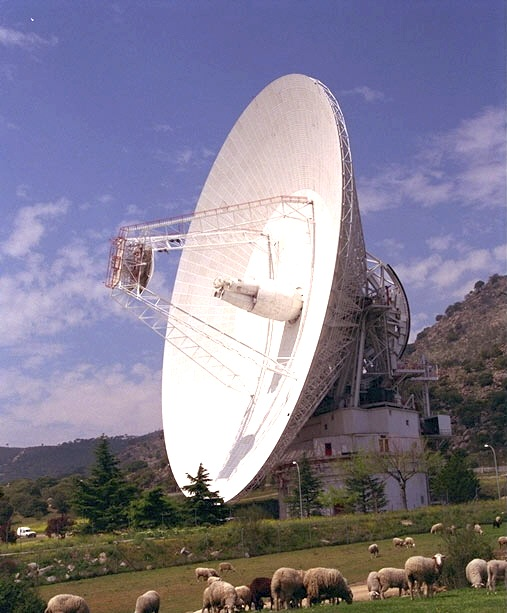
\includegraphics[totalheight=0.45\textheight]
				{fig/DSS-63.jpg}
				\caption[DSS-63 70-meter antenna]
				{
					DSS-63 70-meter antenna at Robledo de Chavela,
					Madrid.
				}
		\label{dss63image}
			\end{center}
		\end{figure}
		
		\begin{table}[tbp]
		\caption[DSS-63 properties, versus other antennas]
		{DSS-63 properties, versus other antennas; values at 22 GHz.}
		\label{dss63comparison}
		\begin{smalltabular}{ccccc} \midrule
				& & \textbf{Aperture} & & \textbf{Sensitivity} \\
		        \textbf{Telescope} & \textbf{Diameter} & \textbf{efficiency
		        ($\mathrm{\eta_a}$)} & \textbf{Resolution} &
		        \textbf{(K/Jy)}\\[4pt] \midrule Effelsberg & 100 m & 29\% & 40’’
		        & 0.8\\ GBT & 100-110 m& 55\% & 34’’ & 1.5\\ Robledo DSS-63 &
		        70 m & 49\% & 42’’ & 0.7\\ 
		\end{smalltabular}
		\end{table}
		
		\begin{table}[tbp]
		\begin{minipage}{\linewidth}
		\caption[Antenna, receiver and spectrometer properties of
		DSS-63]
		{Antenna, receiver and spectrometer properties of DSS-63.}
		\begin{smalltabular}{cl} 
		\multirow{10}*{\minitab[c]{\textbf{Antenna} \\
		\textbf{System}\footnote{HPBW, aperture efficiency, sensitivity and
		pointing accuracy measured at 22GHz, with 40º of elevation}}}
				& \textbf{Name}: Deep Space Station 63 \\
				& \textbf{Diameter}: 70 m \\
				& \textbf{Type}: parabolic Cassegrain \\
				& \textbf{Mount}: azimuth/elevation \\
				& \textbf{Latitude}: 40º 25’ 52’’ N \\
				& \textbf{Longitude}: 04º 14’ 53’’ W \\
				& \textbf{Altitude}: 865.5 m \\
				& \textbf{HPBW}\footnote{Half-Power Beam Width}: 42’’ \\
				& \textbf{Aperture Efficiency ($\eta$)}: 49\% maximum \\
				& \textbf{Sensitivity}: 0.7 K/Jy \\
				& \textbf{Pointing accuracy}: $\leq$ 10'' \\
				\addlinespace\midrule\addlinespace
				
				\multirow{5}*{\minitab[c]{\textbf{K-band} \\
				\textbf{receiver}}} & \textbf{Amplifier type}: cooled HEMT\\
				& \textbf{Frequency range}: 18-26 GHz \\
				& \textbf{Polarization}: LCP\footnote{Left Circular
				Polarisation} or RCP\footnote{Right Circular
				Polarisation}
				(default, LCP) \\
				& \textbf{$\mathbf{T_{sys}}$ (winter)}: 50 K \\
				& \textbf{$\mathbf{T_{sys}}$ (summer)}: 75 K \\
				\addlinespace\midrule\addlinespace

		        \multirow{17}*{\minitab[c]
				{\textbf{Spectrometers}\footnote{The Spaceborne-500
				is the correlator
		        currently in use. It superseded the Spectra-Data,
				the first correlator available in this telescope
				(2001 to 2003), and is no longer in operation.
				The SAO4K, on the other hand, belongs to the
				Smithsonian Astrophysical Observatory, and is used
				for the SAMBA survey.}}} &
		        \textbf{Spaceborne-500}\\ &
		        \textbf{Type}: Digital autocorrelator \\ & \textbf{BW}: 2, 4, 8
		        and 16 MHz\\ & \textbf{Num. channels}: 384\\ &
		        \textbf{Observing mode}: position switching\\
				\addlinespace[3mm]
				
				 &
		        \textbf{Spectra-Data}\\ & \textbf{Type}:
		        Fourier-transform autocorrelator \\ & \textbf{BW}: 1, 2.5, 5
		        and 10 MHz\\ & \textbf{Num. channels}: 256\\ &
		        \textbf{Observing mode}: frequency switching\\
				\addlinespace[3mm]
				&
		        \textbf{SAO4K}\\ & \textbf{Type}: Digital autocorrelator \\ &
		        \textbf{BW}: 400 MHz\\ & \textbf{Num. channels}: 4096\\ &
		        \textbf{Observing mode}: position switching\\ 
		\end{smalltabular}
		\label{dss63properties}
		\end{minipage}
		\end{table}
		
		Each DSCC has at least four operational antennas:

		\begin{itemize}
			\item One 26-meter diameter antenna, originally built
			to support the Apollo missions to the Moon, presently
			used for communicating with Earth-orbiting spacecraft.
			
			 \item One 34-meter diameter high efficiency antenna
			(HEF), designed around a precision-shaped reflector,
			for maximum signal sensitivity.
			
			 \item One 34-meter diameter beam waveguide antenna
			(BWG), based on the HEF design, with five mirrors that
			reflect radio signals along a beam-waveguide tube from
			the antenna vertex to the equipment room, for easier
			maintenance access.
			
			 \item One 70-meter diameter antenna, with the highest
			sensitivity, used for tracking the deepest space
			missions.
		\end{itemize}
		
		In the case of the Madrid DSCC, the 70m antenna is DSS-63,
		whose picture is displayed in figure~\ref{dss63image}.
		Due to their high sensitivity in centimetre wavelengths,
		they can be used to perform astronomical observations,
		when they are not following NASA vehicles .
		
		Of all the time devoted for scientific observations,
		around 3\% of the time at the Canberra and Madrid stations
		(up to 260 hours per year and per antenna) is available to
		Host-Country astronomers. \suppress[Enrique]{The
		organisation responsible for the scheduling of this time at
		Madrid DSCC is the Laboratorio de Astrofísica Espacial y
		Física Fundamental (LAEFF) of the Instituto Nacional de
		Técnica Aeroespacial (INTA), by arrangement with NASA.} The
		organisation responsible for the scheduling of this time at
		Madrid DSCC is the Centro de Astrobiología (INTA-CSIC), by
		arrangement with NASA.
		
		Table~\ref{dss63comparison} compares some properties of
		DSS-63 with those from other astronomically oriented radio
		telescopes, while table~\ref{dss63properties} summarises
		DSS-63 properties of the antenna system, the K-band receiver,
		and the different spectrometers which have been installed at
		the the DSS-63 antenna.
		
		Nowadays, Host Country time at the MDSCC is devoted to
		perform spectroscopic observations at K-band (i.e.,
		wavelengths around 10 cm), with the 70-m DSS-63 antenna.
		In particular, several projects for observing \water{}
		masers have been performed ---see, for intance, Gregorio de
		Monsalvo's thesis~\cite{de-Gregorio-Monsalvo:2006fk}---,
		and the team wished to make those spectroscopic archives
		public.
		
		% subsection spectral_observations_dss63 (fold)
		\subsection{Spectral observations with the DSS-63 antenna}
		\label{sub:spectral_observations_dss63}
			As the main scientific use of the DSS-63 antenna is the
			recollection of spectra, we will describe how
			spectroscopic observations are performed with this
			instrument.
			
			The observing process for a spectrum is as follows:
			
			\begin{description}
				\item[Source selection] First, a target source with
				a medium elevation at the time of observation is
				selected; extreme elevations introduce additional
				pointing errors and/or additional atmospheric
				effects.
				
				\item[Pointing calibrator selection] Once the
				source has been selected, a strong pointing
				calibration source near the target is chosen,
				because minimising antenna motion between pointing
				calibration
				and the actual observation better maintains the
				mirror shape\footnote{Antenna geometry changes
				mostly due to gravitational effects which are
				minimum for changes in azimuth, a much more
				significant for changes in elevation. Large radio
				astronomical antennas are designed following the
				homology principle, so that deformations produce
				changes in focus, so in order to collect the
				maximum flux focus calibrations should be
				performed with sources at the same elevation as
				the source to be observed.}.
				
				\item[Pointing calibration] The antenna will be
				moved up and down in elevation, and clockwise and
				counter-clockwise in cross-elevation, around the
				expected position for the pointing calibrator. As
				the profile for the telescope beam conforms to a
				Gaussian distribution, the data can be fitted with
				a Gaussian, and the pointing error adjusted by
				comparison between the expected position of the
				calibrator, and the fitted maximum flux position.
				This correction will be applied to the coordinates
				where the source is expected to be.
				
				\item[Focus calibration] The same calibrator can be
				used to calibrate the focus of the instrument,
				defined as the position of the secondary mirror
				that maximises the power collected by the
				instrument. Again, the profile for the focus, when
				the mirror is moved along its axis, is assumed to
				be Gaussian, and the fit for the maximum
				provides the focus.
				
				\item[On/Off source observation] Both the source
				and a nearby position with no emissions have to be
				observed, in order to discriminate the contribution
				from the instrument. This is performed either by
				changing the position of the antenna (position
				switching), or by moving the secondary mirror in
				such a way that the main feed is focused on a
				different region of the sky, with no radio sources
				(wobbler switching). Another possibility is to
				compare the power of the emission from the same
				source at slightly different frequencies, assuming
				that the antenna and atmospheric noise does not
				change with this frequency switch (frequency
				switching). In the case of the DSS-63, on/off
				observations are performed either by position
				switching or frequency switching.
				
				\item[Atmospheric corrections] The amount of energy
				received by the instrument depends strongly on
				weather conditions, and on the length of the path
				of the signal through the atmosphere. In
				particular, at cm wavelengths the amount of water
				vapour in the atmosphere is the major contributor
				to atmospheric opacity (a quantity that is
				proportional to the probability of a photon being
				absorbed after travelling a given length in the
				atmosphere). Measurements of opacity at different
				elevations (tipping curves, or skydips), which
				correspond to different air masses (a measure of
				the amount of atmospheric gas in the line of sight
				of the instrument), are used to fit a curve that
				provides the atmospheric opacity\footnote{See
				section 7.2 in \emph{Tools of radio
				astronomy}~\cite{2004tra..book.....R} for
				details.}. This is usually
				done at DSS-63 once per observing session and
				frequency setup.
			\end{description}
			
			There are other corrections and calibrations to
			consider, but most of them can be obtained from typical
			values for the instrument and particular configuration,
			and do not contribute to illustrate the observing
			process with the DSS-63 antenna.
			
			 Of particular interest will be parameters such as
			system temperature ($\mathrm{T_{sys}}$), main beam
			solid angle ($\mathrm{\Omega_{mb}}$), aperture
			efficiency ($\mathrm{\eta_a}$), and the antenna
			temperature scale.
			
			 The data output of the correlator is a 384-sample
			autocorrelation function, which by means of the Fourier
			transform (Discrete Fourier Transform, in this case)
			provides a function proportional to the power spectrum
			of the source\footnote{See section 4.1.2 of \emph{Tools
			of Radio Astronomy}~\cite{2004tra..book.....R} for the
			derivation.}. The post-processing of the observation,
			together with the calibration procedures, will allow us
			to determine the actual spectrum scale, and frequencies
			for the salient features of the spectrum.
			
		% subsection spectral_observations_dss63 (end)
		
		\subsection{Archive requirements} % (fold)
		\label{sub:archive_requirements_dss63}
			
			The archive for the DSS-63 antenna, then, is an
			archive for single-point spectroscopic observations.
			The particular requirements for the archive were:
			
			\begin{description}
				\item[Support for two single-point modes] The
				DSS-63 antenna archive would hold, as per the
				initial specification, only single-point on-off
				spectra using frequency switching, or
				single-point continuum measurements.
				
				\item[VO spectral access services] The main data
				products of the archive are spectra, which are
				supported by the Spectrum Data Model (incorporated
				in the RADAMS, as we have seen), and continuum
				measurements, which are considered to be one-point,
				wide-band spectra, similar to photometric data
				points in the visible band. A SSAP service will
				be implemented on top of the database, as well
				as a ConeSearch on the Scans table.
				
				\item[Web access interface] The web access
				interface would use the same infrastructure needed
				for the SSAP service, but providing a VO compatible
				spectral web-service, instead of using web forms.
				
				\item[No modification to the instrument control
				system] All of the information stored in the
				archive should be available either from ingestion
				of the FITS files, or by harvesting the observation
				logs and control system output, but nothing should
				be added to the instrument control system. This is
				both a precautionary measure, so that we do not
				interfere with the telescope, but also works for
				making the project self-contained: tasks can be
				performed without need for external developers to
				modify another piece of software.
				
				\item[Simple data access policy] The MSDCC data
				standard access policy is the
				straightforward NRAO policy: after 18 months, data
				are available to the public. However, as all data
				to be provided by these archive are older than that,
				there is no actual Policy module for this archive.
			\end{description}
			
		% subsection archive_requirements_dss63 (end)
		
		\subsection{Archive architecture} % (fold)
		\label{sub:archive_architecture_dss63}
			
			\begin{figure}[tbp]
				\begin{center}
					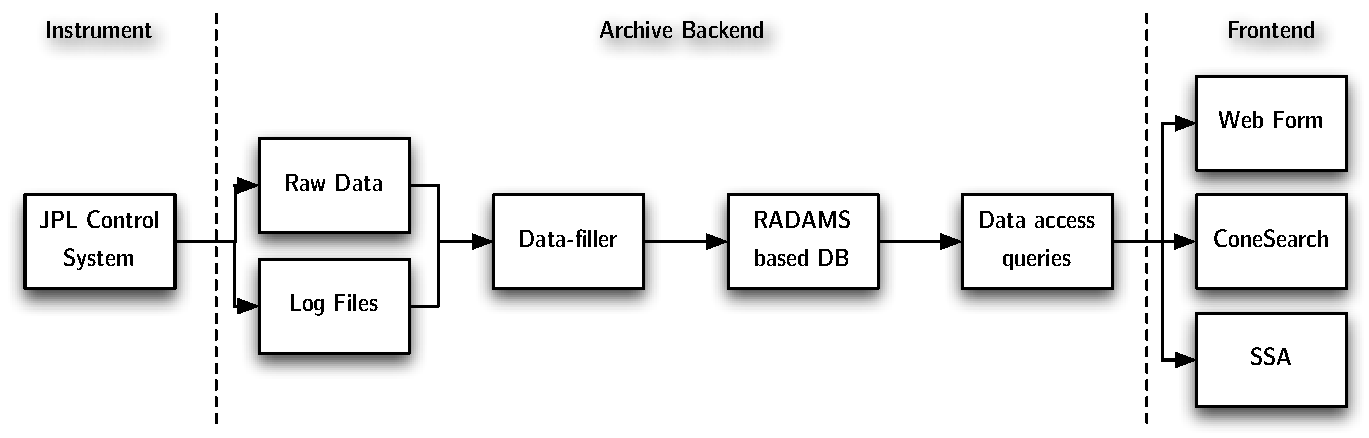
\includegraphics[width=\textwidth]
					{fig/DSS63_ArchiveArchitecture.pdf}
				\end{center}
				\caption[High level, layered architecture for the
				Robledo Archive]
				{High level, layered architecture for the Robledo
				Archive. Dotted lines represent the logical
				separation between layers. Arrows represent data
				flow between sub-systems. Communications between
				layers are confined to the communications
				established between interfacing components.}
				\label{figDss63ArchiveArchitecture}
			\end{figure}
			
			With the requirements above, a layered
			architecture for the archive was devised where each
			layer correspond to a different subsystem:
			
			\begin{description}
				\item[Instrument] With regards to the archive, the
				Instrument is represented by the Instrument Control
				System, which provides the links to observational
				data and configuration metadata.
				

				\item[Archive Backend] The backend of the archive 
				(not to be confused with any of the instrument’s
				back-ends) is the module responsible for database
				and metadata access and maintenance. Includes the
				creation of entries in the database from the Raw
				data and observation log files, and the queries for
				supporting different query interfaces.
				
				
				\item[Frontend] This is the actual accessible layer
				for human-computer or computer-computer interaction
				with the Archive Backend, using either a web form
				interface, or VO services such as ConeSearch for
				observation logs, and SSA for obtaining actual
				spectra.
			\end{description}
			
			
			Figure~\ref{figDss63ArchiveArchitecture} shows that
			layered organisation, and how each layer maintains a
			single point of interaction with the next.
			
			\suppress[Juande]{
			One of the most important parts of the system is what
			in that figure is called the Archive Infrastructure,
			which contains the methods for accessing Instrument
			logs, the database following the RADAMS data model
			for the metadata, and the raw data storage.
			
			One of the sub-modules in the Archive Infrastructure
			module is the Data-filler, which waits for messages
			from the Instrument (in the form of entries on the
			observation log), and ingests them into the database,
			with links to the raw data storage.}
			
			We have detailed several subsystems within the 
			Archive Backend: the Data-filler, which waits for messages
			from the Instrument (in the form of entries on the
			observation log), ingesting them into the database,
			with links to the raw data storage; the database itself,
			which as we will see conforms to the RADAMS; and
			the archive queries to support the different use cases.
			
			Apart from the automatic operation mode, the Data-filler
			can
			also be launched on its own, providing it with a set of
			FITS files to ingest, and the observing logs making
			reference to those FITS files.
			
			For this archive, we have developed the complete Archive
			Backend, including the database implementation, which
			has been developed using the
			Django\urlnote{http://www.djangoproject.com/}
			Python-based development framework. The database being
			used is Oracle, as per CAB prescriptions, and the user
			interface and VO data access modules built on top of
			the RADAMS will be developed by the SVO members of the
			LAEFF.
			
			An interesting feature of the Archive Backend for the
			DSS-63 antenna, which has been also implemented for
			the IRAM~30m, is the way VO-related metadata (UCDs,
			UTypes, and other IVOA vocabularies) are provided 
			to the Data access queries. We will describe that
			mechanism when discussing the implementation details
			of the IRAM~30m archive.
			
		% subsection archive_architecture_dss63 (end)
		
		\subsection{RADAMS implementation} % (fold)
		\label{sub:radams_implementation_dss63}
			\newcommand{\dsssixtythreesqlurl}
			{http://www.iaa.es/~jdsant/thesis/dss63-sourceDM-v0_5.sql}
			
			Figure~\ref{fig:fig_DSS63-data-model} shows the
			different database tables and their
			relationships\footnote {The complete \texttt{.sql} file
			implementing tables and relationships can be found
			at:\\ \url{\dsssixtythreesqlurl}.} used for the actual
			implementation of the DSS-63 archive.
			
			If we compare that figure with the high-level overview
			of the RADAMS ---figure~\ref{RADAMSHLoverview}---, we
			can see that in the archive implementation there are
			many more dependencies on the Observation or ObsData
			related tables in the archive database than those shown
			for the RADAMS.
			
			That is so because we need to be able to perform
			different direct relationships with scans, as different
			search capabilities would be unfeasible if the whole
			dependency tree had to be traversed. However, in order
			to describe an observation (scan) or a set of
			associated scans, those additional dependencies are
			implicit, and need not be stated, as is the case with
			the high-level RADAMS data model.
			
			\suppress[Juande]
			{listing~\ref{lst:dss63-sql} shows the beginning of the
			SQL statements which define the data model and table
			layout, and provide a link to the complete SQL file.}
			
			\begin{figure}[tbp]
				\centering
					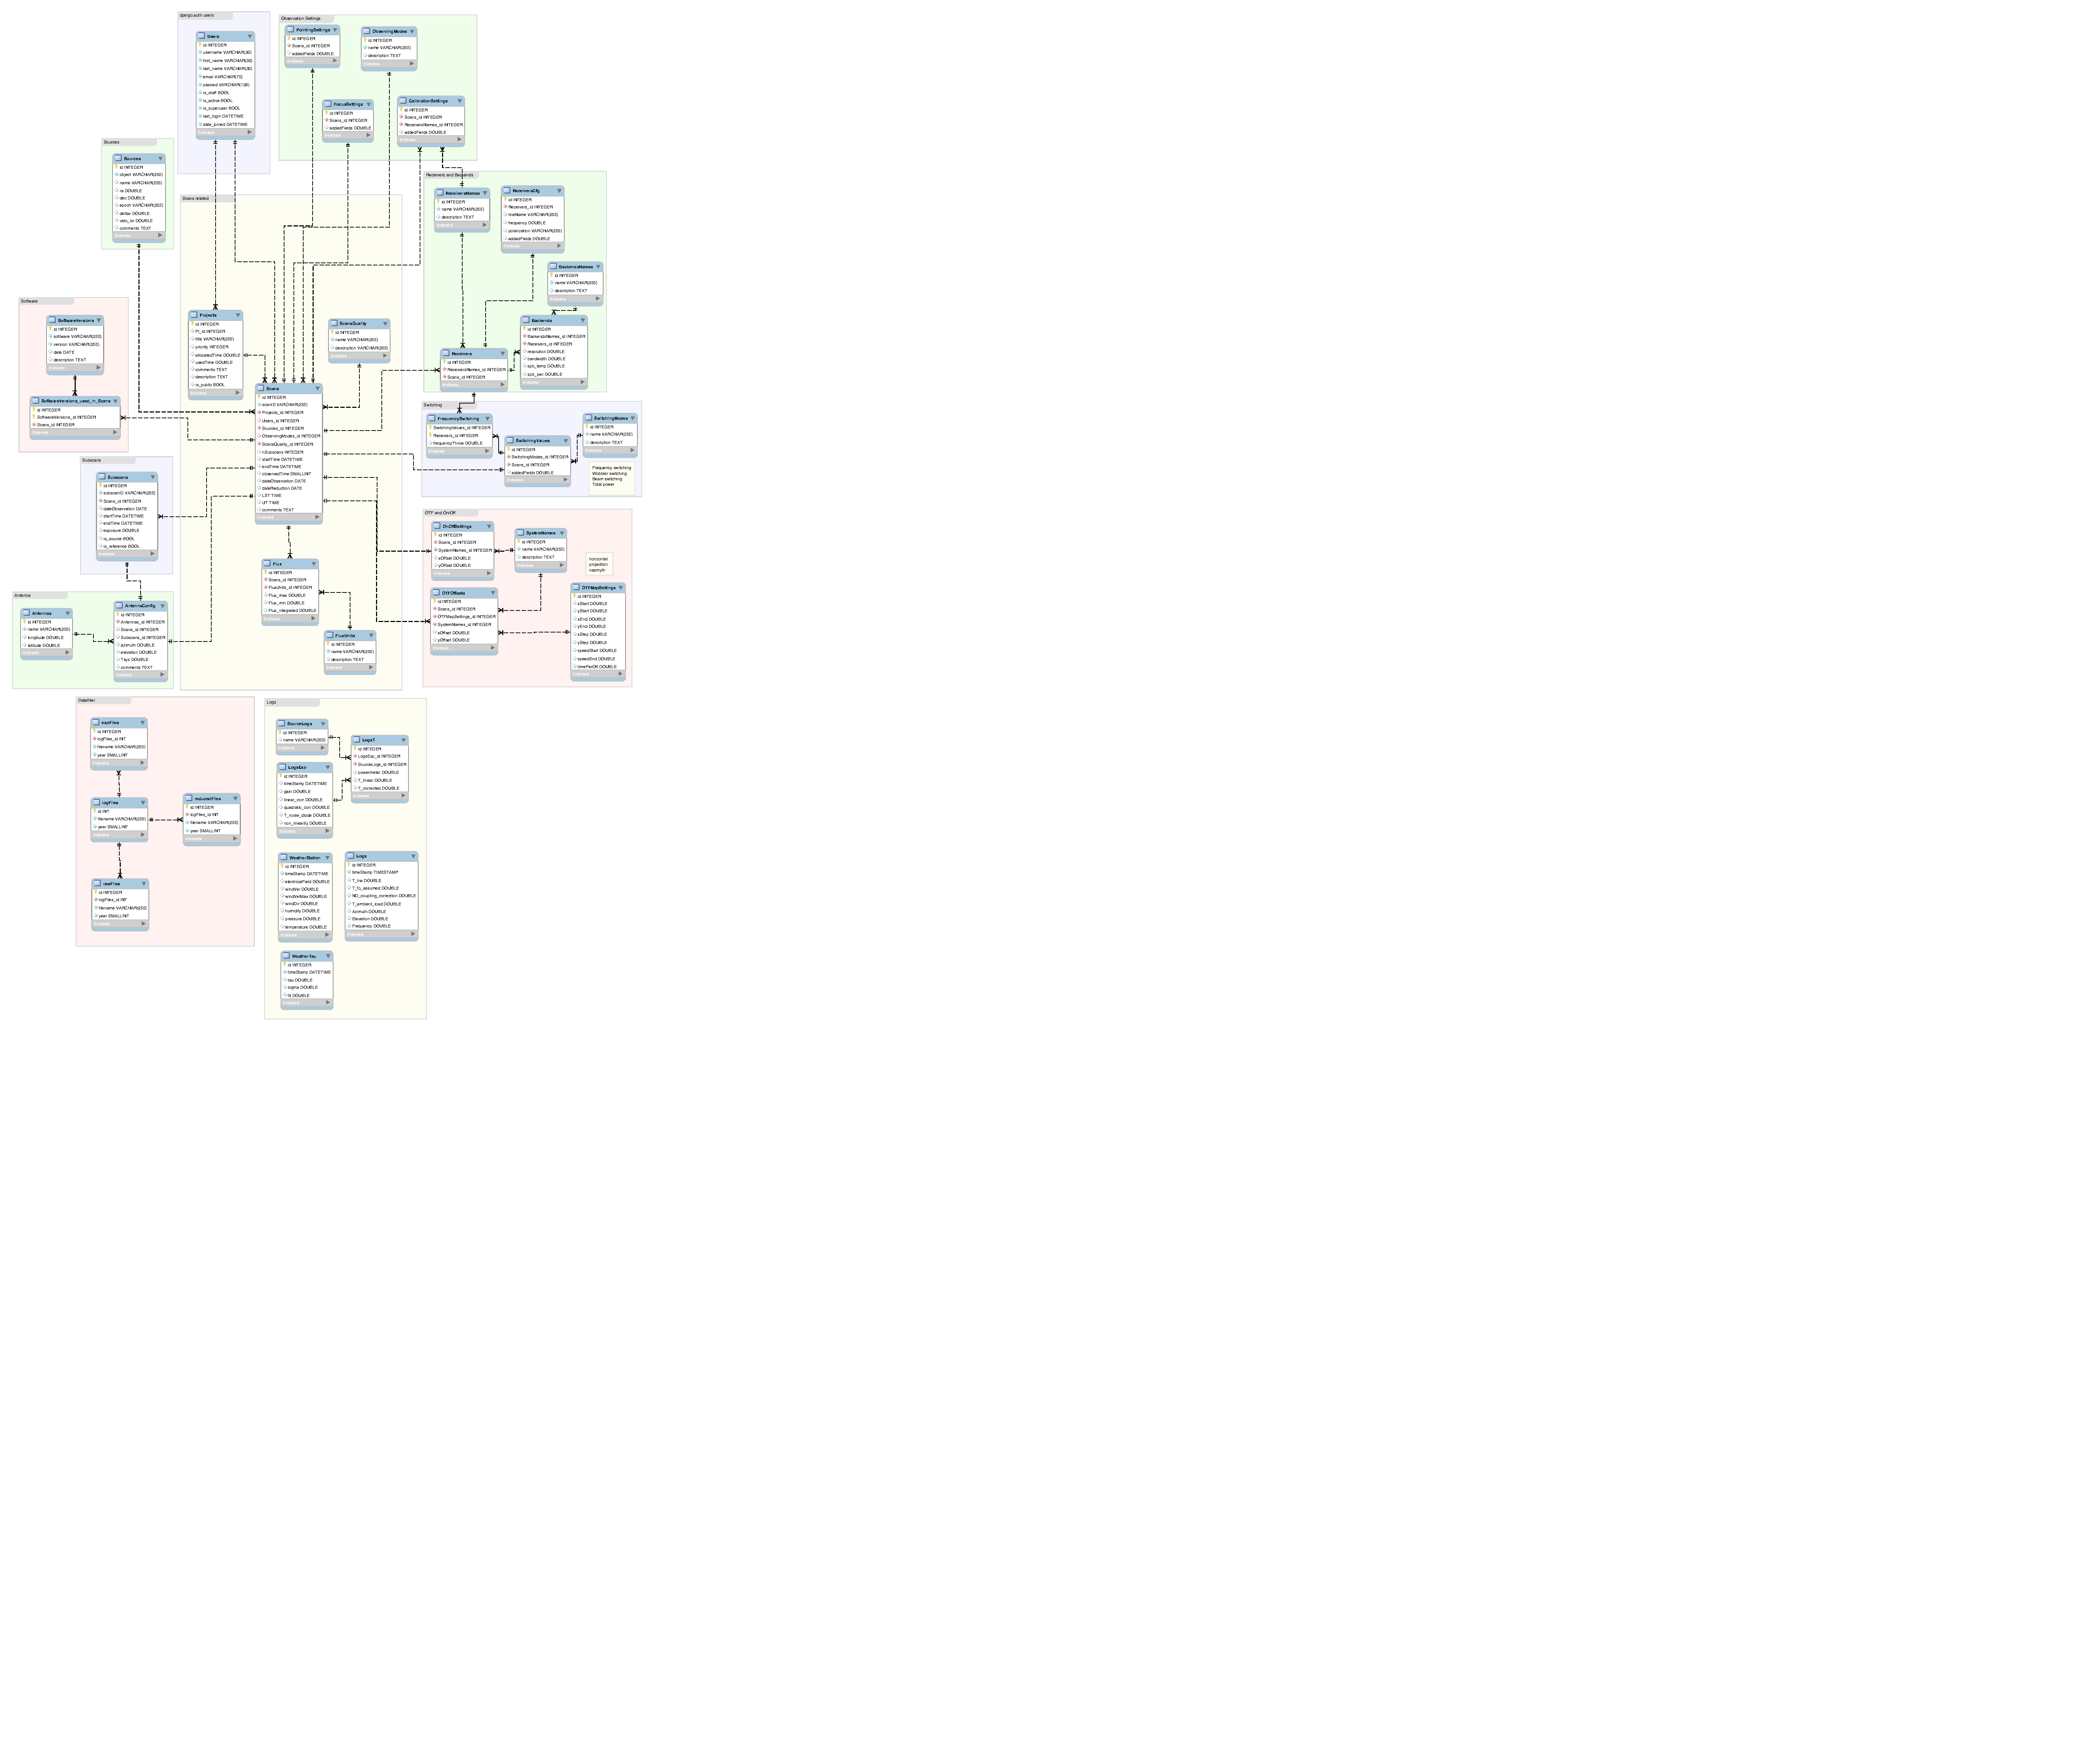
\includegraphics[totalheight=1.1\textheight]
					{fig/DSS63-dm.pdf}
				\caption[Implementation of the data model for the
				DSS-63 archive]
				{
					Implementation of the data model for the
					DSS-63 archive, generated from the actual
					SQL \method{CREATE TABLE} statements.
				}
				\label{fig:fig_DSS63-data-model}
			\end{figure}
			
			The Scan object is the cornerstone for
			all observations, as we discussed in
			section~\ref{subObsDataCharacterisation}. From the
			Scan entity, all other relationships derive, except
			for those having to do with the Data-filler
			configuration ---which are themselves outside of the
			scope of the RADAMS---, and data which are related to
			Scans only by simultaneity, as is the case for
			weather station readings, whose only relation to
			Scans is their timestamp.
			
			Sources implements a very simplified Target data model.
			
			Project metadata is directly related to observations
			as part of the Curation data model, and to Users.
			Project and Users would be used by the Policy algorithm
			if DSS-63 archive's policy were not fixed, as
			previously stated.
			
			The Observations Settings, Receivers and Backends,
			Switching, Antenna and observation Settings are the
			tables supporting
			the Provenance.Instrument data model. Many of the tables
			are tables for instrument codes, or instrument setting
			codes.
			
			The major mismatch between the RADAMS data model
			(developed for VO data query, and data description)
			and the actual data stored in the database (retrieved
			from the data available through the FITS file headers,
			and from the instrument control system), is found in
			the Characterisation data model: metadata such as
			spatial resolution, spectral resolution, et cetera,
			are derived from the values of the observation
			settings, and are not to be stored with the database,
			but will be, instead, generated on the fly by the
			VO interfaces. We will revisit this peculiarity when
			describing the IRAM~30m archive database and its
			relationship to the RADAMS.
			
			\begin{figure}[tbp]
				\centering
					\includegraphics[width=\textwidth]
					{fig/DSS63_searchForm.pdf}
				\caption{
					Prototype search form for the DSS-63 archive.
				}
				\label{fig:fig_DSS63_searchForm}
			\end{figure}
			
			The prototype web form interface to the archive
			can bee seen in figure~\ref{fig:fig_DSS63_searchForm},
			where the Target data model (and CharDM Spatial axis)
			is queried by the Source name and position search box,
			the Project search box queries Observation metadata,
			Observation date is related to the CharDM in the
			Temporal axis, and Frequency/Velocity and Line names
			perform their searches on the CharDM Spectral and
			Velocity axes.
			
			\suppress[Juande]{
			\lstinputlisting[
				language=SQL,
				caption={[SQL statements for Robledo data model]
				First SQL statements for Robledo data model.
				The complete SQL file can be downloaded from the
				following link:\\
				\url{\dsssixtythreesqlurl}
				},
				label=lst:dss63-sql,
				firstline=1,
				lastline=65,
				float=tbp
			]
			{listing/dss63-sourceDM-v0_5.sql}
			
			In order to be able to compare the RADAMS with the
			actual SQL files, the following pages are devoted to
			show all tables and attributes, with data types,
			ability to hold null files and default values.
			
			Table primary keys are in \textbf{\emph{bold italics}},
			while unique fields are in \textbf{bold}.
			
			\clearpage
			
			% phpMyAdmin LaTeX Dump
% version 2.11.7.1
% http://www.phpmyadmin.net
%
% Servidor: localhost
% Tiempo de generación: 25-03-2009 a las 22:24:51
% Versión del servidor: 5.0.41
% Versión de PHP: 5.2.6
% 
% Base de datos: 'dss63'
% 

%
% Estructura: antennaconfig
%
 \begin{longtable}{lcccl}
 
 \caption{Structure of table \texttt{antennaconfig}} \label{tab:antennaconfig-structure} \\
 \textbf{Field} & \textbf{Type} & \textbf{Null} & \textbf{Default}  \\ \midrule
\endfirsthead
 \caption*{Structure of table \texttt{antennaconfig} (continued)} \\ 
 \addlinespace \textbf{Field} & \textbf{Type} & \textbf{Null} & \textbf{Default}  \\ \midrule \endhead \endfoot 
\textbf{\textit{id}} & int(11) & Yes & NULL \\ \addlinespace 
Antennas\_id & int(11) & Yes &  \\ \addlinespace 
Scans\_id & int(11) & Yes & NULL \\ \addlinespace 
Subscans\_id & int(11) & Yes & NULL \\ \addlinespace 
azimuth & double & Yes & NULL \\ \addlinespace 
elevation & double & Yes & NULL \\ \addlinespace 
Tsys & double & Yes & NULL \\ \addlinespace 
comments & longtext & Yes &  \\ 
 \end{longtable}

%
% Estructura: antennas
%
 \begin{longtable}{lcccl}
 
 \caption{Structure of table \texttt{antennas}} \label{tab:antennas-structure} \\
 \addlinespace \textbf{Field} & \textbf{Type} & \textbf{Null} & \textbf{Default}  \\ \midrule
\endfirsthead
 \caption*{Structure of table \texttt{antennas} (continued)} \\ 
 \addlinespace \textbf{Field} & \textbf{Type} & \textbf{Null} & \textbf{Default}  \\ \midrule \endhead \endfoot 
\textbf{\textit{id}} & int(11) & Yes & NULL \\ \addlinespace 
name & varchar(255) & Yes &  \\ \addlinespace 
longitude & double & Yes & NULL \\ \addlinespace 
latitude & double & Yes & NULL \\ 
\end{longtable}

%
% Estructura: backends
%
 \begin{longtable}{lcccl}
 
 \caption{Structure of table \texttt{backends}} \label{tab:backends-structure} \\
 \addlinespace \textbf{Field} & \textbf{Type} & \textbf{Null} & \textbf{Default}  \\ \midrule
\endfirsthead
 \caption*{Structure of table \texttt{backends} (continued)} \\ 
 \addlinespace \textbf{Field} & \textbf{Type} & \textbf{Null} & \textbf{Default}  \\ \midrule \endhead \endfoot 
\textbf{\textit{id}} & int(11) & Yes & NULL \\ \addlinespace 
BackendsNames\_id & int(11) & Yes &  \\ \addlinespace 
Receivers\_id & int(11) & Yes &  \\ \addlinespace 
resolution & double & Yes & NULL \\ \addlinespace 
bandwidth & double & Yes & NULL \\ \addlinespace 
spb\_temp & double & Yes & NULL \\ \addlinespace 
spb\_pwr & double & Yes & NULL \\ 
  \end{longtable}

%
% Estructura: backendsnames
%
 \begin{longtable}{lcccl}
 
 \caption{Structure of table \texttt{backendsnames}} \label{tab:backendsnames-structure} \\
 \addlinespace \textbf{Field} & \textbf{Type} & \textbf{Null} & \textbf{Default}  \\ \midrule
\endfirsthead
 \caption*{Structure of table \texttt{backendsnames} (continued)} \\ 
 \addlinespace \textbf{Field} & \textbf{Type} & \textbf{Null} & \textbf{Default}  \\ \midrule \endhead \endfoot 
\textbf{\textit{id}} & int(11) & Yes & NULL \\ \addlinespace 
name & varchar(255) & Yes &  \\ \addlinespace 
description & longtext & Yes &  \\ 
  \end{longtable}

%
% Estructura: calibrationsettings
%
 \begin{longtable}{lcccl}
 
 \caption{Structure of table \texttt{calibrationsettings}} \label{tab:calibrationsettings-structure} \\
 \addlinespace \textbf{Field} & \textbf{Type} & \textbf{Null} & \textbf{Default}  \\ \midrule
\endfirsthead
 \caption*{Structure of table \texttt{calibrationsettings} (continued)} \\ 
 \addlinespace \textbf{Field} & \textbf{Type} & \textbf{Null} & \textbf{Default}  \\ \midrule \endhead \endfoot 
\textbf{\textit{id}} & int(11) & Yes & NULL \\ \addlinespace 
Scans\_id & int(11) & Yes &  \\ \addlinespace 
Receivers\_id & int(11) & Yes &  \\ 
  \end{longtable}


%
% Estructura: expfiles
%
 \begin{longtable}{lcccl}
 
 \caption{Structure of table \texttt{expfiles}} \label{tab:expfiles-structure} \\
 \addlinespace \textbf{Field} & \textbf{Type} & \textbf{Null} & \textbf{Default}  \\ \midrule
\endfirsthead
 \caption*{Structure of table \texttt{expfiles} (continued)} \\ 
 \addlinespace \textbf{Field} & \textbf{Type} & \textbf{Null} & \textbf{Default}  \\ \midrule \endhead \endfoot 
\textbf{\textit{id}} & int(11) & Yes & NULL \\ \addlinespace 
logFiles\_id & int(11) & Yes &  \\ \addlinespace 
\textbf{filename} & varchar(255) & Yes &  \\ \addlinespace 
year & smallint(6) & Yes &  \\ 
  \end{longtable}

%
% Estructura: flux
%
 \begin{longtable}{lcccl}
 
 \caption{Structure of table \texttt{flux}} \label{tab:flux-structure} \\
 \addlinespace \textbf{Field} & \textbf{Type} & \textbf{Null} & \textbf{Default}  \\ \midrule
\endfirsthead
 \caption*{Structure of table \texttt{flux} (continued)} \\ 
 \addlinespace \textbf{Field} & \textbf{Type} & \textbf{Null} & \textbf{Default}  \\ \midrule \endhead \endfoot 
\textbf{\textit{id}} & int(11) & Yes & NULL \\ \addlinespace 
Scans\_id & int(11) & Yes &  \\ \addlinespace 
FluxUnits\_id & int(11) & Yes &  \\ \addlinespace 
Flux\_max & double & Yes & NULL \\ \addlinespace 
Flux\_min & double & Yes & NULL \\ \addlinespace 
Flux\_integrated & double & Yes & NULL \\ 
  \end{longtable}

%
% Estructura: fluxunits
%
 \begin{longtable}{lcccl}
 
 \caption{Structure of table \texttt{fluxunits}} \label{tab:fluxunits-structure} \\
 \addlinespace \textbf{Field} & \textbf{Type} & \textbf{Null} & \textbf{Default}  \\ \midrule
\endfirsthead
 \caption*{Structure of table \texttt{fluxunits} (continued)} \\ 
 \addlinespace \textbf{Field} & \textbf{Type} & \textbf{Null} & \textbf{Default}  \\ \midrule \endhead \endfoot 
\textbf{\textit{id}} & int(11) & Yes & NULL \\ \addlinespace 
name & varchar(255) & Yes &  \\ \addlinespace 
description & longtext & Yes &  \\ 
  \end{longtable}

%
% Estructura: focussettings
%
 \begin{longtable}{lcccl}
 
 \caption{Structure of table \texttt{focussettings}} \label{tab:focussettings-structure} \\
 \addlinespace \textbf{Field} & \textbf{Type} & \textbf{Null} & \textbf{Default}  \\ \midrule
\endfirsthead
 \caption*{Structure of table \texttt{focussettings} (continued)} \\ 
 \addlinespace \textbf{Field} & \textbf{Type} & \textbf{Null} & \textbf{Default}  \\ \midrule \endhead \endfoot 
\textbf{\textit{id}} & int(11) & Yes & NULL \\ \addlinespace 
Scans\_id & int(11) & Yes &  \\ 
  \end{longtable}

%
% Estructura: frequencyswitching
%
 \begin{longtable}{lcccl}
 
 \caption{Structure of table \texttt{frequencyswitching}} \label{tab:frequencyswitching-structure} \\
 \addlinespace \textbf{Field} & \textbf{Type} & \textbf{Null} & \textbf{Default}  \\ \midrule
\endfirsthead
 \caption*{Structure of table \texttt{frequencyswitching} (continued)} \\ 
 \addlinespace \textbf{Field} & \textbf{Type} & \textbf{Null} & \textbf{Default}  \\ \midrule \endhead \endfoot 
\textbf{\textit{id}} & int(11) & Yes & NULL \\ \addlinespace 
SwitchingValues\_id & int(11) & Yes &  \\ \addlinespace 
Receivers\_id & int(11) & Yes &  \\ \addlinespace 
frequencyThrow & double & Yes & NULL \\ 
  \end{longtable}

%
% Estructura: logfiles
%
 \begin{longtable}{lcccl}
 
 \caption{Structure of table \texttt{logfiles}} \label{tab:logfiles-structure} \\
 \addlinespace \textbf{Field} & \textbf{Type} & \textbf{Null} & \textbf{Default}  \\ \midrule
\endfirsthead
 \caption*{Structure of table \texttt{logfiles} (continued)} \\ 
 \addlinespace \textbf{Field} & \textbf{Type} & \textbf{Null} & \textbf{Default}  \\ \midrule \endhead \endfoot 
\textbf{\textit{id}} & int(11) & Yes & NULL \\ \addlinespace 
\textbf{filename} & varchar(255) & Yes &  \\ \addlinespace 
year & smallint(6) & Yes &  \\ 
  \end{longtable}

%
% Estructura: logs
%
 \begin{longtable}{lcccl}
 
 \caption{Structure of table \texttt{logs}} \label{tab:logs-structure} \\
 \addlinespace \textbf{Field} & \textbf{Type} & \textbf{Null} & \textbf{Default}  \\ \midrule
\endfirsthead
 \caption*{Structure of table \texttt{logs} (continued)} \\ 
 \addlinespace \textbf{Field} & \textbf{Type} & \textbf{Null} & \textbf{Default}  \\ \midrule \endhead \endfoot 
\textbf{\textit{id}} & int(11) & Yes & NULL \\ \addlinespace 
\textbf{timeStamp} & datetime & Yes &  \\ \addlinespace 
T\_lna & double & Yes & NULL \\ \addlinespace 
T\_fo\_assumed & double & Yes & NULL \\ \addlinespace 
ND\_coupling\_correction & double & Yes & NULL \\ \addlinespace 
T\_ambient\_load & double & Yes & NULL \\ \addlinespace 
Azimuth & double & Yes & NULL \\ \addlinespace 
Elevation & double & Yes & NULL \\ \addlinespace 
Frequency & double & Yes & NULL \\ 
  \end{longtable}

%
% Estructura: logsexp
%
 \begin{longtable}{lcccl}
 
 \caption{Structure of table \texttt{logsexp}} \label{tab:logsexp-structure} \\
 \addlinespace \textbf{Field} & \textbf{Type} & \textbf{Null} & \textbf{Default}  \\ \midrule
\endfirsthead
 \caption*{Structure of table \texttt{logsexp} (continued)} \\ 
 \addlinespace \textbf{Field} & \textbf{Type} & \textbf{Null} & \textbf{Default}  \\ \midrule \endhead \endfoot 
\textbf{\textit{id}} & int(11) & Yes & NULL \\ \addlinespace 
\textbf{timeStamp} & datetime & Yes &  \\ \addlinespace 
gain & double & Yes & NULL \\ \addlinespace 
linear\_corr & double & Yes & NULL \\ \addlinespace 
quadratic\_corr & double & Yes & NULL \\ \addlinespace 
T\_noise\_diode & double & Yes & NULL \\ \addlinespace 
non\_linearity & double & Yes & NULL \\ 
  \end{longtable}

%
% Estructura: logst
%
 \begin{longtable}{lcccl}
 
 \caption{Structure of table \texttt{logst}} \label{tab:logst-structure} \\
 \addlinespace \textbf{Field} & \textbf{Type} & \textbf{Null} & \textbf{Default}  \\ \midrule
\endfirsthead
 \caption*{Structure of table \texttt{logst} (continued)} \\ 
 \addlinespace \textbf{Field} & \textbf{Type} & \textbf{Null} & \textbf{Default}  \\ \midrule \endhead \endfoot 
\textbf{\textit{id}} & int(11) & Yes & NULL \\ \addlinespace 
SourceLogs\_id & int(11) & Yes &  \\ \addlinespace 
LogsExp\_id & int(11) & Yes &  \\ \addlinespace 
powermeter & double & Yes & NULL \\ \addlinespace 
T\_linear & double & Yes & NULL \\ \addlinespace 
T\_corrected & double & Yes & NULL \\ 
  \end{longtable}

%
% Estructura: observingmodes
%
 \begin{longtable}{lcccl}
 
 \caption{Structure of table \texttt{observingmodes}} \label{tab:observingmodes-structure} \\
 \addlinespace \textbf{Field} & \textbf{Type} & \textbf{Null} & \textbf{Default}  \\ \midrule
\endfirsthead
 \caption*{Structure of table \texttt{observingmodes} (continued)} \\ 
 \addlinespace \textbf{Field} & \textbf{Type} & \textbf{Null} & \textbf{Default}  \\ \midrule \endhead \endfoot 
\textbf{\textit{id}} & int(11) & Yes & NULL \\ \addlinespace 
name & varchar(255) & Yes &  \\ \addlinespace 
description & longtext & Yes &  \\ 
  \end{longtable}

%
% Estructura: onoffsettings
%
 \begin{longtable}{lcccl}
 
 \caption{Structure of table \texttt{onoffsettings}} \label{tab:onoffsettings-structure} \\
 \addlinespace \textbf{Field} & \textbf{Type} & \textbf{Null} & \textbf{Default}  \\ \midrule
\endfirsthead
 \caption*{Structure of table \texttt{onoffsettings} (continued)} \\ 
 \addlinespace \textbf{Field} & \textbf{Type} & \textbf{Null} & \textbf{Default}  \\ \midrule \endhead \endfoot 
\textbf{\textit{id}} & int(11) & Yes & NULL \\ \addlinespace 
Scans\_id & int(11) & Yes &  \\ \addlinespace 
SystemNames\_id & int(11) & Yes &  \\ \addlinespace 
xOffset & double & Yes & NULL \\ \addlinespace 
yOffset & double & Yes & NULL \\ 
  \end{longtable}

%
% Estructura: otfmapsettings
%
 \begin{longtable}{lcccl}
 
 \caption{Structure of table \texttt{otfmapsettings}} \label{tab:otfmapsettings-structure} \\
 \addlinespace \textbf{Field} & \textbf{Type} & \textbf{Null} & \textbf{Default}  \\ \midrule
\endfirsthead
 \caption*{Structure of table \texttt{otfmapsettings} (continued)} \\ 
 \addlinespace \textbf{Field} & \textbf{Type} & \textbf{Null} & \textbf{Default}  \\ \midrule \endhead \endfoot 
\textbf{\textit{id}} & int(11) & Yes & NULL \\ \addlinespace 
xStart & double & Yes & NULL \\ \addlinespace 
yStart & double & Yes & NULL \\ \addlinespace 
xEnd & double & Yes & NULL \\ \addlinespace 
yEnd & double & Yes & NULL \\ \addlinespace 
xStep & double & Yes & NULL \\ \addlinespace 
yStep & double & Yes & NULL \\ \addlinespace 
speedStart & double & Yes & NULL \\ \addlinespace 
speedEnd & double & Yes & NULL \\ \addlinespace 
timePerOtf & double & Yes & NULL \\ 
  \end{longtable}

%
% Estructura: otfoffsets
%
 \begin{longtable}{lcccl}
 
 \caption{Structure of table \texttt{otfoffsets}} \label{tab:otfoffsets-structure} \\
 \addlinespace \textbf{Field} & \textbf{Type} & \textbf{Null} & \textbf{Default}  \\ \midrule
\endfirsthead
 \caption*{Structure of table \texttt{otfoffsets} (continued)} \\ 
 \addlinespace \textbf{Field} & \textbf{Type} & \textbf{Null} & \textbf{Default}  \\ \midrule \endhead \endfoot 
\textbf{\textit{id}} & int(11) & Yes & NULL \\ \addlinespace 
Scans\_id & int(11) & Yes &  \\ \addlinespace 
OTFMapSettings\_id & int(11) & Yes &  \\ \addlinespace 
SystemNames\_id & int(11) & Yes &  \\ \addlinespace 
xOffset & double & Yes & NULL \\ \addlinespace 
yOffset & double & Yes & NULL \\ 
  \end{longtable}

%
% Estructura: pointingsettings
%
 \begin{longtable}{lcccl}
 
 \caption{Structure of table \texttt{pointingsettings}} \label{tab:pointingsettings-structure} \\
 \addlinespace \textbf{Field} & \textbf{Type} & \textbf{Null} & \textbf{Default}  \\ \midrule
\endfirsthead
 \caption*{Structure of table \texttt{pointingsettings} (continued)} \\ 
 \addlinespace \textbf{Field} & \textbf{Type} & \textbf{Null} & \textbf{Default}  \\ \midrule \endhead \endfoot 
\textbf{\textit{id}} & int(11) & Yes & NULL \\ \addlinespace 
Scans\_id & int(11) & Yes &  \\ 
  \end{longtable}

%
% Estructura: projects
%
 \begin{longtable}{lcccl}
 
 \caption{Structure of table \texttt{projects}} \label{tab:projects-structure} \\
 \addlinespace \textbf{Field} & \textbf{Type} & \textbf{Null} & \textbf{Default}  \\ \midrule
\endfirsthead
 \caption*{Structure of table \texttt{projects} (continued)} \\ 
 \addlinespace \textbf{Field} & \textbf{Type} & \textbf{Null} & \textbf{Default}  \\ \midrule \endhead \endfoot 
\textbf{\textit{id}} & int(11) & Yes & NULL \\ \addlinespace 
PI\_id & int(11) & Yes & NULL \\ \addlinespace 
\textbf{title} & varchar(255) & Yes &  \\ \addlinespace 
priority & smallint(6) & Yes & NULL \\ \addlinespace 
allocatedTime & double & Yes & NULL \\ \addlinespace 
usedTime & double & Yes & NULL \\ \addlinespace 
comments & longtext & Yes &  \\ \addlinespace 
description & longtext & Yes &  \\ \addlinespace 
is\_public & tinyint(1) & Yes &  \\ 
  \end{longtable}

%
% Estructura: rawfiles
%
 \begin{longtable}{lcccl}
 
 \caption{Structure of table \texttt{rawfiles}} \label{tab:rawfiles-structure} \\
 \addlinespace \textbf{Field} & \textbf{Type} & \textbf{Null} & \textbf{Default}  \\ \midrule
\endfirsthead
 \caption*{Structure of table \texttt{rawfiles} (continued)} \\ 
 \addlinespace \textbf{Field} & \textbf{Type} & \textbf{Null} & \textbf{Default}  \\ \midrule \endhead \endfoot 
\textbf{\textit{id}} & int(11) & Yes & NULL \\ \addlinespace 
logFiles\_id & int(11) & Yes &  \\ \addlinespace 
\textbf{filename} & varchar(255) & Yes &  \\ \addlinespace 
year & smallint(6) & Yes &  \\ 
  \end{longtable}

%
% Estructura: receivers
%
 \begin{longtable}{lcccl}
 
 \caption{Structure of table \texttt{receivers}} \label{tab:receivers-structure} \\
 \addlinespace \textbf{Field} & \textbf{Type} & \textbf{Null} & \textbf{Default}  \\ \midrule
\endfirsthead
 \caption*{Structure of table \texttt{receivers} (continued)} \\ 
 \addlinespace \textbf{Field} & \textbf{Type} & \textbf{Null} & \textbf{Default}  \\ \midrule \endhead \endfoot 
\textbf{\textit{id}} & int(11) & Yes & NULL \\ \addlinespace 
ReceiversNames\_id & int(11) & Yes &  \\ \addlinespace 
Scans\_id & int(11) & Yes &  \\ 
  \end{longtable}

%
% Estructura: receiverscfg
%
 \begin{longtable}{lcccl}
 
 \caption{Structure of table \texttt{receiverscfg}} \label{tab:receiverscfg-structure} \\
 \addlinespace \textbf{Field} & \textbf{Type} & \textbf{Null} & \textbf{Default}  \\ \midrule
\endfirsthead
 \caption*{Structure of table \texttt{receiverscfg} (continued)} \\ 
 \addlinespace \textbf{Field} & \textbf{Type} & \textbf{Null} & \textbf{Default}  \\ \midrule \endhead \endfoot 
\textbf{\textit{id}} & int(11) & Yes & NULL \\ \addlinespace 
Receivers\_id & int(11) & Yes &  \\ \addlinespace 
linename & varchar(255) & Yes &  \\ \addlinespace 
frequency & double & Yes & NULL \\ \addlinespace 
polarization & varchar(255) & Yes &  \\ 
  \end{longtable}

%
% Estructura: receiversnames
%
 \begin{longtable}{lcccl}
 
 \caption{Structure of table \texttt{receiversnames}} \label{tab:receiversnames-structure} \\
 \addlinespace \textbf{Field} & \textbf{Type} & \textbf{Null} & \textbf{Default}  \\ \midrule
\endfirsthead
 \caption*{Structure of table \texttt{receiversnames} (continued)} \\ 
 \addlinespace \textbf{Field} & \textbf{Type} & \textbf{Null} & \textbf{Default}  \\ \midrule \endhead \endfoot 
\textbf{\textit{id}} & int(11) & Yes & NULL \\ \addlinespace 
name & varchar(255) & Yes &  \\ \addlinespace 
description & longtext & Yes &  \\ 
  \end{longtable}

%
% Estructura: reducedfiles
%
 \begin{longtable}{lcccl}
 
 \caption{Structure of table \texttt{reducedfiles}} \label{tab:reducedfiles-structure} \\
 \addlinespace \textbf{Field} & \textbf{Type} & \textbf{Null} & \textbf{Default}  \\ \midrule
\endfirsthead
 \caption*{Structure of table \texttt{reducedfiles} (continued)} \\ 
 \addlinespace \textbf{Field} & \textbf{Type} & \textbf{Null} & \textbf{Default}  \\ \midrule \endhead \endfoot 
\textbf{\textit{id}} & int(11) & Yes & NULL \\ \addlinespace 
logFiles\_id & int(11) & Yes &  \\ \addlinespace 
\textbf{filename} & varchar(255) & Yes &  \\ \addlinespace 
year & smallint(6) & Yes &  \\ 
  \end{longtable}

%
% Estructura: scans
%
 \begin{longtable}{lcccl}
 
 \caption{Structure of table \texttt{scans}} \label{tab:scans-structure} \\
 \addlinespace \textbf{Field} & \textbf{Type} & \textbf{Null} & \textbf{Default}  \\ \midrule
\endfirsthead
 \caption*{Structure of table \texttt{scans} (continued)} \\ 
 \addlinespace \textbf{Field} & \textbf{Type} & \textbf{Null} & \textbf{Default}  \\ \midrule \endhead \endfoot 
\textbf{\textit{id}} & int(11) & Yes & NULL \\ \addlinespace 
\textbf{scanID} & varchar(255) & Yes &  \\ \addlinespace 
Projects\_id & int(11) & Yes &  \\ \addlinespace 
Users\_id & int(11) & Yes & NULL \\ \addlinespace 
Sources\_id & int(11) & Yes &  \\ \addlinespace 
ObservingModes\_id & int(11) & Yes & NULL \\ \addlinespace 
ScansQuality\_id & int(11) & Yes &  \\ \addlinespace 
nSubscans & smallint(6) & Yes & NULL \\ \addlinespace 
startTime & datetime & Yes & NULL \\ \addlinespace 
endTime & datetime & Yes & NULL \\ \addlinespace 
observedTime & smallint(6) & Yes & NULL \\ \addlinespace 
dateObservation & date & Yes & NULL \\ \addlinespace 
dateReduction & date & Yes & NULL \\ \addlinespace 
LST & time & Yes & NULL \\ \addlinespace 
UT & time & Yes & NULL \\ \addlinespace 
comments & longtext & Yes &  \\ 
  \end{longtable}

%
% Estructura: scansquality
%
 \begin{longtable}{lcccl}
 
 \caption{Structure of table \texttt{scansquality}} \label{tab:scansquality-structure} \\
 \addlinespace \textbf{Field} & \textbf{Type} & \textbf{Null} & \textbf{Default}  \\ \midrule
\endfirsthead
 \caption*{Structure of table \texttt{scansquality} (continued)} \\ 
 \addlinespace \textbf{Field} & \textbf{Type} & \textbf{Null} & \textbf{Default}  \\ \midrule \endhead \endfoot 
\textbf{\textit{id}} & int(11) & Yes & NULL \\ \addlinespace 
name & varchar(255) & Yes &  \\ \addlinespace 
description & longtext & Yes &  \\ 
  \end{longtable}

%
% Estructura: softwareversions
%
 \begin{longtable}{lcccl}
 
 \caption{Structure of table \texttt{softwareversions}} \label{tab:softwareversions-structure} \\
 \addlinespace \textbf{Field} & \textbf{Type} & \textbf{Null} & \textbf{Default}  \\ \midrule
\endfirsthead
 \caption*{Structure of table \texttt{softwareversions} (continued)} \\ 
 \addlinespace \textbf{Field} & \textbf{Type} & \textbf{Null} & \textbf{Default}  \\ \midrule \endhead \endfoot 
\textbf{\textit{id}} & int(11) & Yes & NULL \\ \addlinespace 
software & varchar(255) & Yes &  \\ \addlinespace 
version & varchar(255) & Yes &  \\ \addlinespace 
date & date & Yes & NULL \\ \addlinespace 
description & longtext & Yes &  \\ 
  \end{longtable}

%
% Estructura: softwareversions_used_in_scans
%
 \begin{longtable}{lcccl}
 
 \caption{Structure of table \texttt{softwareversions\_used\_in\_scans}} \label{tab:softwareversions_used_in_scans-structure} \\
 \addlinespace \textbf{Field} & \textbf{Type} & \textbf{Null} & \textbf{Default}  \\ \midrule
\endfirsthead
 \caption*{Structure of table \texttt{softwareversions\_used\_in\_scans} (continued)} \\ 
 \addlinespace \textbf{Field} & \textbf{Type} & \textbf{Null} & \textbf{Default}  \\ \midrule \endhead \endfoot 
\textbf{\textit{id}} & int(11) & Yes & NULL \\ \addlinespace 
\textbf{scans\_id} & int(11) & Yes &  \\ \addlinespace 
\textbf{softwareversions\_id} & int(11) & Yes &  \\ 
  \end{longtable}

%
% Estructura: sourcelogs
%
 \begin{longtable}{lcccl}
 
 \caption{Structure of table \texttt{sourcelogs}} \label{tab:sourcelogs-structure} \\
 \addlinespace \textbf{Field} & \textbf{Type} & \textbf{Null} & \textbf{Default}  \\ \midrule
\endfirsthead
 \caption*{Structure of table \texttt{sourcelogs} (continued)} \\ 
 \addlinespace \textbf{Field} & \textbf{Type} & \textbf{Null} & \textbf{Default}  \\ \midrule \endhead \endfoot 
\textbf{\textit{id}} & int(11) & Yes & NULL \\ \addlinespace 
name & varchar(255) & Yes &  \\ 
  \end{longtable}

%
% Estructura: sources
%
 \begin{longtable}{lcccl}
 
 \caption{Structure of table \texttt{sources}} \label{tab:sources-structure} \\
 \addlinespace \textbf{Field} & \textbf{Type} & \textbf{Null} & \textbf{Default}  \\ \midrule
\endfirsthead
 \caption*{Structure of table \texttt{sources} (continued)} \\ 
 \addlinespace \textbf{Field} & \textbf{Type} & \textbf{Null} & \textbf{Default}  \\ \midrule \endhead \endfoot 
\textbf{\textit{id}} & int(11) & Yes & NULL \\ \addlinespace 
object & varchar(255) & Yes &  \\ \addlinespace 
name & varchar(255) & Yes &  \\ \addlinespace 
ra & double & Yes & NULL \\ \addlinespace 
dec & double & Yes & NULL \\ \addlinespace 
epoch & varchar(20) & Yes &  \\ \addlinespace 
deltav & double & Yes & NULL \\ \addlinespace 
velo\_lsr & double & Yes & NULL \\ \addlinespace 
comments & longtext & Yes &  \\ 
  \end{longtable}

%
% Estructura: subscans
%
 \begin{longtable}{lcccl}
 
 \caption{Structure of table \texttt{subscans}} \label{tab:subscans-structure} \\
 \addlinespace \textbf{Field} & \textbf{Type} & \textbf{Null} & \textbf{Default}  \\ \midrule
\endfirsthead
 \caption*{Structure of table \texttt{subscans} (continued)} \\ 
 \addlinespace \textbf{Field} & \textbf{Type} & \textbf{Null} & \textbf{Default}  \\ \midrule \endhead \endfoot 
\textbf{\textit{id}} & int(11) & Yes & NULL \\ \addlinespace 
\textbf{subscanID} & varchar(255) & Yes &  \\ \addlinespace 
Scans\_id & int(11) & Yes &  \\ \addlinespace 
dateObservation & date & Yes & NULL \\ \addlinespace 
startTime & datetime & Yes & NULL \\ \addlinespace 
endTime & datetime & Yes & NULL \\ \addlinespace 
exposure & double & Yes & NULL \\ \addlinespace 
is\_source & tinyint(1) & Yes & NULL \\ \addlinespace 
is\_reference & tinyint(1) & Yes & NULL \\ 
  \end{longtable}

%
% Estructura: switchingmodes
%
 \begin{longtable}{lcccl}
 
 \caption{Structure of table \texttt{switchingmodes}} \label{tab:switchingmodes-structure} \\
 \addlinespace \textbf{Field} & \textbf{Type} & \textbf{Null} & \textbf{Default}  \\ \midrule
\endfirsthead
 \caption*{Structure of table \texttt{switchingmodes} (continued)} \\ 
 \addlinespace \textbf{Field} & \textbf{Type} & \textbf{Null} & \textbf{Default}  \\ \midrule \endhead \endfoot 
\textbf{\textit{id}} & int(11) & Yes & NULL \\ \addlinespace 
name & varchar(255) & Yes &  \\ \addlinespace 
description & longtext & Yes &  \\ 
  \end{longtable}

%
% Estructura: switchingvalues
%
 \begin{longtable}{lcccl}
 
 \caption{Structure of table \texttt{switchingvalues}} \label{tab:switchingvalues-structure} \\
 \addlinespace \textbf{Field} & \textbf{Type} & \textbf{Null} & \textbf{Default}  \\ \midrule
\endfirsthead
 \caption*{Structure of table \texttt{switchingvalues} (continued)} \\ 
 \addlinespace \textbf{Field} & \textbf{Type} & \textbf{Null} & \textbf{Default}  \\ \midrule \endhead \endfoot 
\textbf{\textit{id}} & int(11) & Yes & NULL \\ \addlinespace 
SwitchingModes\_id & int(11) & Yes &  \\ \addlinespace 
Scans\_id & int(11) & Yes &  \\ 
  \end{longtable}

%
% Estructura: systemnames
%
 \begin{longtable}{lcccl}
 
 \caption{Structure of table \texttt{systemnames}} \label{tab:systemnames-structure} \\
 \addlinespace \textbf{Field} & \textbf{Type} & \textbf{Null} & \textbf{Default}  \\ \midrule
\endfirsthead
 \caption*{Structure of table \texttt{systemnames} (continued)} \\ 
 \addlinespace \textbf{Field} & \textbf{Type} & \textbf{Null} & \textbf{Default}  \\ \midrule \endhead \endfoot 
\textbf{\textit{id}} & int(11) & Yes & NULL \\ \addlinespace 
name & varchar(255) & Yes &  \\ \addlinespace 
description & longtext & Yes &  \\ 
  \end{longtable}

%
% Estructura: weatherstation
%
 \begin{longtable}{lcccl}
 
 \caption{Structure of table \texttt{weatherstation}} \label{tab:weatherstation-structure} \\
 \addlinespace \textbf{Field} & \textbf{Type} & \textbf{Null} & \textbf{Default}  \\ \midrule
\endfirsthead
 \caption*{Structure of table \texttt{weatherstation} (continued)} \\ 
 \addlinespace \textbf{Field} & \textbf{Type} & \textbf{Null} & \textbf{Default}  \\ \midrule \endhead \endfoot 
\textbf{\textit{id}} & int(11) & Yes & NULL \\ \addlinespace 
\textbf{timeStamp} & datetime & Yes &  \\ \addlinespace 
electricalField & double & Yes & NULL \\ \addlinespace 
windVel & double & Yes & NULL \\ \addlinespace 
windVelMax & double & Yes & NULL \\ \addlinespace 
windDir & double & Yes & NULL \\ \addlinespace 
humidity & double & Yes & NULL \\ \addlinespace 
pressure & double & Yes & NULL \\ \addlinespace 
temperature & double & Yes & NULL \\ 
  \end{longtable}

%
% Estructura: weathertau
%
 \begin{longtable}{lcccl}
 
 \caption{Structure of table \texttt{weathertau}} \label{tab:weathertau-structure} \\
 \addlinespace \textbf{Field} & \textbf{Type} & \textbf{Null} & \textbf{Default}  \\ \midrule
\endfirsthead
 \caption*{Structure of table \texttt{weathertau} (continued)} \\ 
 \addlinespace \textbf{Field} & \textbf{Type} & \textbf{Null} & \textbf{Default}  \\ \midrule \endhead \endfoot 
\textbf{\textit{id}} & int(11) & Yes & NULL \\ \addlinespace 
\textbf{timeStamp} & datetime & Yes &  \\ \addlinespace 
tau & double & Yes & NULL \\ \addlinespace 
sigma & double & Yes & NULL \\ \addlinespace 
fit & double & Yes & NULL \\ 
  \end{longtable}

			}
			
		% subsection radams_implementation_dss63 (end)
	% section the_robledo_dss_63_archive (end)
	
	\section{The IRAM~30m archive} % (fold)
	\label{sec:the_iram_30m_archive}
		
		The IRAM~30m radio telescope, located at the Loma de Dílar,
		in the shoulders of the Pico Veleta in Sierra Nevada,
		Granada, is the leading millimetre-range radio telescope,
		due to its sensitivity and instrument capabilities. One
		objective measure of its importance is that it has generated
		more
		than 1100 papers since 1982\footnote{Source:
		List of publications till 2008 making use of the IRAM~30m
		compiled by former IRAM-Spain director Rai\-ner
		Mauers\-ber\-ger till 2008, and published through the
		SAO/NASA Astrophysics Data System:\\
		\url{\rainerirampubsurl}}, when it started operations.
		
		\begin{figure}[tbp]
			\begin{center}
				\includegraphics[width=\textwidth]
				{fig/IRAM_30m.jpg}
				\caption[IRAM 30-meter antenna.]
				{
					IRAM 30-meter antenna, next to the residential
					and control building, near Pico
					Veleta (visible on the right side of the
					picture), at Sierra Nevada, Granada. Picture by
					the author.
				}
		\label{fig:iram30m}
			\end{center}
		\end{figure}
		
		
		The IRAM~30m ---shown on figure~\ref{fig:iram30m} next
		to the residence and control building--- hosts several
		instruments, both coherent (heterodyne) and incoherent
		(bolometers), with different data reduction packages and
		techniques. There are also single-pixel and multi-pixel
		detectors, what makes the data handling even more
		particular.
		
		As the data from the detectors can be fed to several
		analysis systems, the former are called front-ends, while
		the latter are called back-ends. Keeping the different
		frontend-backend combinations is one of the complications
		of data storage for the IRAM~30m.
		
		And apart from the different frontend-backend combinations,
		one of the most complex parts of data handling for
		astronomical observatories is the handling of observing
		modes, compounded in radio astronomy with the combination
		of switching modes. They have been compiled, and briefly
		explained, in table~\ref{tabIRAM30mObservingSwitchingModes}.
		The definitive guide to the different observing modes,
		switching modes, front-ends, backends, and observing setup,
		is the guide to the IRAM New Control System (NCS) user
		interface\urlnote{\irampakourl}~\cite{2007pako.iram..109U}.
		
		\renewcommand{\tabularxcolumn}[1]{m{#1}}
		\begin{table}[tp]
		\begin{minipage}{\linewidth}
			\caption[Observing and switching modes of the IRAM~30m]
			{
				Available combinations of observing and switching
				modes at the IRAM~30m telescope. See notes
				and discussion on the text.
			}
			\label{tabIRAM30mObservingSwitchingModes}
		\begin{center}
		\begin{small}
		\begin{tabularx}{\linewidth}
			{>{\raggedleft\arraybackslash}m{3.25cm} cccc}
			
			\textbf{Observing mode} & 
			\textbf{swTotal}\footnote{In total power observations
			there is, in fact, no switching. See exception at psw
			switching.} &
			\textbf{swBeam}\footnote{In beam switching, the optical
			path is cut several times per observing cycle by the
			periodic interposition of a rotating blade (chopper).
			\invisiblenote{The
			off-source observation allows the estimation of the
			noise in the circuit.}} &
			\textbf{swWobbler}\footnote{In wobbler switching
			observations, the secondary mirror
			\invisiblenote{(the one monted
			on the quadrupod)} \emph{wobbles}, changing inclination
			slightly, effectively switching the beam to a different
			sky position.
			\invisiblenote{The off position changes during time
			around the source, due to the altazimuthal mount
			of the radio telescope.}} &
			\textbf{swFreq}\footnote{In frequency switching
			observations, the same position in the sky is observed
			at different frequencies.
			\invisiblenote{The emission of the source is
			expected to decrease at higher frequencies, while sky
			noise is maintained.}} \\ \midrule
		
			Calibrate (Heterodyne)\footnote{Calibrate observations
			are performed for heterodyne receivers in order to be
			able to convert from voltages/counts to fluxes.
			\invisiblenote
			{This is performed by observing the sky, a calibration
			load at ambient temperature, and a calibration load at
			about the temperature of liquid nitrogen.}} & 
			X & & & \\\addlinespace
			
			Pointing\footnote{Pointing observations are done to
			optimise the positioning of the telescope in Azimuth and
			Elevation.  This is done by continuum
			observations of a cross scan in azimuth and elevation on
			a point source \invisiblenote{(or at least a small
			source)} near the
			intended target source.
			\invisiblenote{The different switching modes
			correspond to different instrument setups, and should
			be the same as for the subsequent observations.}} &
			X &
			X &
			X & \\\addlinespace
		
			Focus\footnote{Focus observations are done to minimise
			the spread of received energy, maximising the collected
			energy. \invisiblenote{They are performed in the same
			switching mode
			as the Pointing and actual observations will be
			performed.}} &
			X &
			X &
			X & \\\addlinespace
		
			Tip (Skydip)\footnote{Tip, antenna tipping, or
			\emph{skydip} observations are performed in order to
			estimate the actual opacity of the atmosphere at
			different air masses (amount of atmosphere in the
			line of sight). \invisiblenote{This is more important for
			bolometer receivers, as heterodyne receivers can
			estimate opacity from their own observations.}} &
			X & & &
			\\\addlinespace
		
			Track\footnote{In Track or Tracking observations
			the position of the antenna does not change in celestial
			coordinates, and the off-source reference is taken by
			switching receiver frequency. \invisiblenote{This is
			particularly useful
			for estimating a line emission against continuum.
			if other line (astronomical or
			atmospherical) is present the observation is useless}} & 
			  &  &  & X \\\addlinespace
		
			On-Off\footnote{Observations made by comparison on
			the signal from a source and from a zero emission
			reference.} &
			psw\footnote{psw: Position switching, where the antenna
			drifts from the on to the off position. For total power
			observations, the complete power patter during the drift
			is also recorded.} & &
			X\invisible{wsw} & \\\addlinespace
		
			OTF Map (Heterodyne)\footnote{On-The-Fly observations
			record antenna signal across a drift in space along
			pre-determined paths. For heterodyne receivers, it
			creates data cubes.} & 
			X & & &
			X \\\addlinespace
		
			%Raster \\\addlinespace
		
			OTF Map (MAMBO Bolometer)\footnote{On-The-Fly
			observations with bolometers create intensity maps
			by recording intensities along pre-determined paths.} & & &
			X & \\\addlinespace
		
			VLBI\footnote{VLBI (Very Long Baseline Interferometry) 
			observations \invisiblenote{require special equipment,
			and} are not
			stored by the IRAM.\invisiblenote{instead are handled
			by the VLBI consortium.}} &
			X \\
		\end{tabularx}
		\end{small}
		\end{center}
		\end{minipage}
		\end{table}
		
		\subsection{Archive architecture} % (fold)
		\label{sub:archive_architecture_iram30}
			
			The architecture of the IRAM~30m archive is very similar
			to that of the DSS-63 archive, and follows the same
			principles of independence from the control system
			operation (in this case, the IRAM NCS), and of 
			layering of dependencies/responsibilities.
			Figure~\ref{figIramArchiveArchitecture} shows that
			architecture, and can be easily compared with
			figure~\ref{figDss63ArchiveArchitecture}
			
			\begin{figure}[tbp]
				\begin{center}
					\includegraphics[width=\textwidth]
					{fig/IRAM30m_ArchiveArchitecture.pdf}
				\end{center}
				\caption[High level, layered architecture for the
				IRAM~30m archive]
				{High level, layered architecture of the 
				archive for the IRAM~30m antenna. Dotted lines
				represent the logical separation between layers.
				Arrows represent data flow between sub-systems.
				Communications between layers are confined to the
				communications established between interfacing
				components.}
				\label{figIramArchiveArchitecture}
			\end{figure}
			
			The differences in the workflow and working
			architecture between the DSS-63 and IRAM~30m are
			essentially related to the difference in the control
			system: whereas the JPL control system used by all
			DSS antennas provides FITS files in a format common
			to al DSCCs, and other JPL sites, together with
			text logs in the same format, the IRAM~30m uses since
			2005 the New Control System~\cite{2007pako.iram..109U,
			Brunswig:2002ul, Brunswig:2004gf, Hily-Blant:2001ve,
			Perrigouard:2005rz, Ungerechts:2002hl}, a Python-based
			real time telescope control system which writes each
			scan in a different IRAM Multi-Beam
			FITS~\cite{MudPolHat0512Multi-Beam} file, while at the
			same each observation is described in an XML
			file~\cite{Brunswig:2004gf}.
			
		% subsection archive_architecture_iram30 (end)
		
		\subsection{RADAMS implementation} % (fold)
		\label{sub:radams_implementation_iram}
			
			Given that the high-level architecture is
			largely the same for both archives, the differences
			between them have to deal with the different
			source data format (JPL FITS versus IMB-FITS), 
			observation logs (JPL text logs versus NCS XML files),
			and different database for supporting the additional
			observing modes, switching modes, and instruments
			available at the IRAM~30m.
			
			This additional complexity could be easily imagined by
			comparing table~\ref{tabIRAM30mObservingSwitchingModes}
			to the observation description for DSS-63 made in
			subsection~\ref{sub:spectral_observations_dss63}: the
			observing modes possible with DSS-63 are just those
			available for heterodyne receivers, and 
			wobbler-switching is not available.
			
			\begin{figure}[tbp]
				\centering
					\includegraphics[totalheight=1.1\textheight]
					{fig/tapas-dm.pdf}
				\caption[Implementation of the data model for the
				IRAM~30m archive]
				{
					Implementation of the data model for the
					IRAM~30 archive, TAPAS (Telescope Archive
					for Public Access System). Generated by reverse
					engineering of the MySQL database.
				}
				\label{fig:fig_iram30m-data-model}
			\end{figure}
			
			Figure~\ref{fig:fig_iram30m-data-model} shows the
			database tables and relationships for the IRAM~30m
			database, named TAPAS (Telescope Archive for
			Public Access System). If we compare it with the DSS-63
			database in figure~\ref{fig:fig_DSS63-data-model}, we
			can see there are many more observing setting tables
			(each one holding different data for each different
			observing mode), and many more Project and Policy
			tables, in order to connect the archived data with the
			existing Pool database\footnote{The Pool database is a
			parallel system used to record project data for
			observing projects to be managed under \emph{pool}
			mode, that is, not having a fixed observing block, but
			instead allocating observing blocks following priority
			criteria for observable sources at any given time,
			using backup projects with less stringent weather
			conditions when high-priority projects cannot be
			observed.}.
			
			Given the higher complexity of the TAPAS database, we
			will perform a detailed comparison of RADAMS entities
			with the archive tables.
			
			\begin{description}
				\item[Observation] Observation is the root class for
				the data model, and serves to bind together all
				related information data and metadata. As such,
				it can be thought of as being embodied by the
				Scans table, with the caveats mentioned before
				about the extra number of dependencies.

				\item[ObsData] ObsData is a proxy to the actual
				observation data. In the case of TAPAS, these are
				raw and reduced IMB-FITS files. A separate table,
				stFileLocations, is used to contain the prefix
				path to where data will actually be located
				(accessible from the TAPAS system). As TAPAS file
				names are systematic\footnote{The file name is of
				the form
				\texttt{iram30-backend-yyyymmddsnn-imb.fits}, where
				backend represents the backend name (i.e.,
				\texttt{wilma}, \texttt{4mhz}, \texttt{vespa}...);
				\texttt{yyyymmdd} represents a date in
				year-month-day format; and \texttt{nn} is the scan
				number, separated from the date by an \texttt{s}.
				An example filename:
				\texttt{iram30m-vespa-20090211s62-imb.fits}}, they
				are built from Scan metadata and the
				stFileLocations table on the fly.

				\item[Target] Describes the target of the observation,
				providing as much information as available for
				already known targets, as discussed in
				section~\ref{subTargetDesc}.
				
				This part of RADAMS is supported in TAPAS by the
				tables ObservedSources and PredefinedSources
				tables.  PredefinedSources contains the sources
				which have been proposed for an observing project,
				and are linked to it\footnote{There is a CALIB 
				observation project in which usual flux, focus
				and pointing calibration sources are included.},
				while ObservedSources
				contains the sources which have actually been
				observed, with the target-related observation
				settings required. In the case of ObservedSources,
				coordinates are given in a generic spherical system
				which is converted into equatorial or other
				systems following the basisSystem and projection
				settings.
				
				Both tables are joined to a SourceRadialVelocities
				tables where recession velocities for well-known
				sources are stored, in order to properly set
				Velocity measurements.

				\item[Characterisation] This is the core of the
				RADAMS and generic observation models, and
				corresponds fully to the Characterisation data
				model Recommendation~\cite{2008dmadcrept.....L},
				as we have discussed in
				section~\ref{subObsDataCharacterisation}.
				
				We will describe separately the origin of
				Characterisation data for each of the axes:
				Spatial, Temporal, Spectral, and Observable.
				
				\begin{description}
					\item[Spatial] For most single-dish
					observations, Location, Bounds and Support
					are the same, and will be taken from the
					relationship between the Scans table and
					the PredefinedSources and ObservedSources
					tables. For OTF mapping, Location is
					taken from the PredefinedSources table,
					while Bounds will be calculated from
					projections of the \mapkey{xStart},
					\mapkey{yStart}, \mapkey{xEnd} and
					\mapkey{yEnd} derived from the ObservedSources
					metadata, while if Support is to be specified
					it has to be calculated from the \mapkey{xStep} 
					and \mapkey{yStep} attributes. For bolometer
					mapping, the Bounds and Support are the
					same\footnote{Support could be defined as a
					2D function on the RMS achieved across the map.},
					but they should be computed by the reduction
					software, or approximated by a convolution of
					observed coordinates  with beam widths.
					
					The coordinate computations for the observations
					have also to take into account the Offsets table,
					as those offsets can be added by the observer
					(following observing project instructions) to 
					use the same observing scripts to scan an offset
					part of the sky. See section 6.1 of the
					\emph{paKo user's
					guide}~\cite{2007pako.iram..109U} for a
					discussion of NCS-supported coordinate systems.
					
					Regarding spatial Resolution, this is a function
					of Antenna, Secondary, Observing mode, Receivers
					and Backends, and is looked up from engineering
					databases.
					
					For spatial accuracy, all data for pointing
					corrections is collected for all scans, and
					statistically studied by the engineering team.
					The Antenna table contains the intended and
					actual elevation and azimuth of the antenna,
					which allows for taking into account the
					average tracking system error, while parameters
					\mapkey{p1} to \mapkey{p9} of the IRAM pointing
					model~\cite{2000SPIE.4015..632P} are also stored,
					and can be used to optimise the pointing model.
					In particular, the observer adds the pointing
					corrections to the Antenna \mapkey{p2} ---azimuth
					correction--- and \mapkey{p7} ---elevation
					correction--- attributes.
					
					
					\item[Temporal] Location in the Temporal axis
					will be defined as the Scan \mapkey{startTime}
					attribute, with Bounds taken from
					\mapkey{startTime} and mapkey{endTime}. In order
					to provide Support the dead times between Scans
					should be calculated, but are not provided.
					
					\item[Spectral] The RADAMS defines the Location
					in the Spectral axis as the frequency for the
					central sample of the spectrum, which
					corresponds to the \mapkey{frequency} attribute
					of the ReceiversCfg table. Bounds are defined
					as that frequency, plus/minus half the
					\mapkey{bandwidth} attribute. Most of the metadata
					for the root AxisFrame.Spectral class is also
					recovered from the ReceiversCfg table.
					The Sensitivity will be compiled from the
					engineering measurements for the receiver, and
					will not be stored in TAPAS, while Resolution
					is compiled from the \mapkey{resolution}
					attribute in the Backends table.
					
					SamplingPrecision is also a function of the
					Backend, and will be stored and looked up from
					a static table.
					
					\item[Observable] For flux observations, such
					as On/Off observations, Location is taken
					from the \mapkey{flux} attribute of
					ObservedSource, while bounds is taken to be
					the interval at that value plus/minus the
					\mapkey{actualRMS} value. We do not provide
					Support for the Observable axis, while
					flux resolution is calculated as \mapkey{flux}
					divided by \mapkey{actualRMS}.
					
					As for flux accuracy, the values should be
					computed from statistics on historical data
					one the TAPAS database is in operation for at
					least a whole semester.
				\end{description}

				\item[Provenance] We will study the implementation
				of Provenance separately for each sub-model:
				
				\begin{description}
					\item[Provenance.Instrument] This part of
					Provenance was discussed in
					section~\ref{sec:instrumental_provenance}. It
					was defined as a hierarchical tree aggregating
					different subsystem configurations:
					Instrument\-Conf could hold several
					Antenna\-Conf entries (for describing
					antenna arrays), one or several Feeds per
					Antenna\-Conf, and one Bean\-Conf per
					Feed stating Beam properties, Receiver
					properties, Spectrum properties and
					Velocity properties.
					
					In TAPAS, the specific Instrument, Location
					and Instrument\-Conf classes are pre-computed
					and stored outside of the TAPAS database.
					The Antenna description part of the RADAMS
					needed to be updated for the IRAM~30m, and
					include the different switching modes, the
					configuration of the Secondary mirror (needed
					for wobbler switching modes). Beam metadata
					needs to be looked up in engineering
					configuration tables, and Receiver,
					Spectrum, and Velocity settings are obtained
					from the Receivers and Backends tables.
					
					
					\item[Provenance.AmbientConditions] This
					part of the RADAMS is directly linked to
					the WeatherStation and WeatherTau tables,
					using timestamps to correlate scans with
					measurements.
					
					In addition, the OpacityCurve is directly
					obtained from the results of observations
					of Tip kind\footnote{Scans with
					\mapkey{stObservingModes\_id} attribute
					corresponding to Tip or Bolotip observations.}.
					The CalibrationResults table holds that
					information for heterodyne receivers, reduced
					with the MIRA package.
					
					
					\item[Provenance.Processing] Some parts of
					Provenance.Processing are implemented on the
					TAPAS database, in particular the Software
					package-related metadata. The calibration
					part is still being reviewed, as different
					packages (MIRA, MOPSIC) provide very
					different processing and calibration
					information. 
					
					
				\end{description}

				\item[Curation] This part of the RADAMS is described
				in section~\ref{sec:curation}. The common curation
				data for TAPAS (the Curation table) is held outside
				of this database, and will be used for creating the
				ConeSearch entry in VO Registries. Project and
				DataID are obtained from the Scans and Project
				tables.
				
				There are plans to link the existing Proposal
				handling database to  the TAPAS system, and in that
				case the remaining Curation data model will be
				implemented.

				\item[Policy] As mentioned in
				section~\ref{sec:policy}, the Policy determination
				algorithm needs to get access to Users, Project,
				and observation related information such as
				Observers, Operators, et cetera.
				
				In TAPAS, Project information is stored in the
				Project table, with a link to the Principal
				Investigator, while Scan holds the Observer
				identifier, and Operators and Observatory staff have
				entries in the DjangoUsers table with the
				\mapkey{isStaff} set to true.
				
				The main difference with the proposed RADAMS
				architecture is that Operators are not identified
				with observations, and that there is no possibility
				to specify Co-Investigators.

				\item[Packaging] The TAPAS archive has all the
				infrastructure needed for being able to provide
				data in the form of VO services. However, due to the
				actual IRAM Policy statement, only header information
				will be publicly available for observations, after
				a 12 years proprietary period, while data themselves
				will only be available for a selection of projects,
				and only after 18 months proprietary period.
				The actual implementation of the Packaging class
				has not been, therefore, adapted to the TAPAS
				archive.
			\end{description}
			
			
			
			
			\newcommand{\iramthirtymetersqlurl}
		{http://www.iaa.es/~jdsant/thesis/iram30m-sourceDM-v0_8.sql}
			The complete SQL file implementing the IRAM~30m archive
			data base can be downloaded from the
			following link:\\
			\url{\iramthirtymetersqlurl}
			
			\suppress[Juande]
			{
			Listing~\ref{lst:iram30m-sql} shows the first SQL
			statements for the Django based archive.
			
			\lstinputlisting[
				language=SQL,
				caption={[SQL statements for IRAM~30m archive data
				model]
				First SQL statements for the IRAM~30m data model.
				
				},
				label=lst:iram30m-sql,
				firstline=1,
				lastline=65,
				float=tbp
			]
			{listing/iram30m-sourceDM-v0_8.sql}
			
			In order to be able to compare the RADAMS with the
			actual database for the IRAM~30m, the following pages
			are devoted to show all tables and attributes, with
			data types, ability to hold null files and default
			values.
			
			Table primary keys are in \textbf{\emph{bold italics}},
			while unique fields are in \textbf{bold}.
			
			\clearpage
			
			% phpMyAdmin LaTeX Dump
% version 2.11.7.1
% http://www.phpmyadmin.net
%
% Servidor: localhost
% Tiempo de generación: 25-03-2009 a las 22:22:56
% Versión del servidor: 5.0.41
% Versión de PHP: 5.2.6
% 
% Base de datos: 'IRAM30m'
% 

%
% Estructura: Antenna
%

\begin{longtable}{lcccl}
 
 \caption{Structure of table \texttt{Antenna}} \label{tab:Antenna-structure} \\
 \addlinespace \textbf{Field} & \textbf{Type} & \textbf{Null} & \textbf{Default}  \\ \midrule
\endfirsthead
 \caption*{Structure of table \texttt{Antenna} (continued)} \\ 
 \addlinespace \textbf{Field} & \textbf{Type} & \textbf{Null} & \textbf{Default}  \\ \midrule \endhead \endfoot
\textbf{\textit{id}} & int(11) & Yes & NULL \\ \addlinespace 
scan\_id & int(11) & Yes &  \\ \addlinespace 
actualAz & double & Yes & NULL \\ \addlinespace 
actualEl & double & Yes & NULL \\ \addlinespace 
trackAz & double & Yes & NULL \\ \addlinespace 
trackEl & double & Yes & NULL \\ \addlinespace 
p2 & double & Yes & NULL \\ \addlinespace 
p4 & double & Yes & NULL \\ \addlinespace 
p5 & double & Yes & NULL \\ \addlinespace 
p7 & double & Yes & NULL \\  
\end{longtable}

%
% Estructura: Backends
%
 \begin{longtable}{lcccl}
 
 \caption{Structure of table \texttt{Backends}} \label{tab:Backends-structure} \\
 \addlinespace \textbf{Field} & \textbf{Type} & \textbf{Null} & \textbf{Default}  \\ \midrule
\endfirsthead
 \caption*{Structure of table \texttt{Backends} (continued)} \\ 
 \addlinespace \textbf{Field} & \textbf{Type} & \textbf{Null} & \textbf{Default}  \\ \midrule \endhead \endfoot
\textbf{\textit{id}} & int(11) & Yes & NULL \\ \addlinespace 
bkName\_id & int(11) & Yes &  \\ \addlinespace 
receiver\_id & int(11) & Yes &  \\ \addlinespace 
receiver2\_id & int(11) & Yes & NULL \\ \addlinespace 
nPart & int(11) & Yes & NULL \\ \addlinespace 
resolution & double & Yes & NULL \\ \addlinespace 
bandwith & double & Yes & NULL \\ \addlinespace 
fShift & double & Yes & NULL \\ \addlinespace 
mode & varchar(36) & Yes &  \\ \addlinespace 
percentage & double & Yes & NULL \\  
 \end{longtable}

%
% Estructura: Basebands
%
 \begin{longtable}{lcccl}
 
 \caption{Structure of table \texttt{Basebands}} \label{tab:Basebands-structure} \\
 \addlinespace \textbf{Field} & \textbf{Type} & \textbf{Null} & \textbf{Default}  \\ \midrule
\endfirsthead
 \caption*{Structure of table \texttt{Basebands} (continued)} \\ 
 \addlinespace \textbf{Field} & \textbf{Type} & \textbf{Null} & \textbf{Default}  \\ \midrule \endhead \endfoot
\textbf{\textit{id}} & int(11) & Yes & NULL \\ \addlinespace 
backend\_id & int(11) & Yes &  \\ \addlinespace 
fSkyStart & double & Yes & NULL \\ \addlinespace 
resolutionFrecuency & double & Yes & NULL \\ \addlinespace 
nChannels & int(11) & Yes & NULL \\  
 \end{longtable}

%
% Estructura: CalibrationSettings
%
 \begin{longtable}{lcccl}
 
 \caption{Structure of table \texttt{CalibrationSettings}} \label{tab:CalibrationSettings-structure} \\
 \addlinespace \textbf{Field} & \textbf{Type} & \textbf{Null} & \textbf{Default}  \\ \midrule
\endfirsthead
 \caption*{Structure of table \texttt{CalibrationSettings} (continued)} \\ 
 \addlinespace \textbf{Field} & \textbf{Type} & \textbf{Null} & \textbf{Default}  \\ \midrule \endhead \endfoot
\textbf{\textit{id}} & int(11) & Yes & NULL \\ \addlinespace 
scan\_id & int(11) & Yes &  \\ \addlinespace 
doAmbient & tinyint(1) & Yes & NULL \\ \addlinespace 
doCold & tinyint(1) & Yes & NULL \\ \addlinespace 
doSky & tinyint(1) & Yes & NULL \\ \addlinespace 
skyOffset\_id & int(11) & Yes & NULL \\ \addlinespace 
gainimagerx & int(11) & Yes & NULL \\ \addlinespace 
doGrid & tinyint(1) & Yes & NULL \\  
 \end{longtable}

%
% Estructura: FocusSettings
%
 \begin{longtable}{lcccl}
 
 \caption{Structure of table \texttt{FocusSettings}} \label{tab:FocusSettings-structure} \\
 \addlinespace \textbf{Field} & \textbf{Type} & \textbf{Null} & \textbf{Default}  \\ \midrule
\endfirsthead
 \caption*{Structure of table \texttt{FocusSettings} (continued)} \\ 
 \addlinespace \textbf{Field} & \textbf{Type} & \textbf{Null} & \textbf{Default}  \\ \midrule \endhead \endfoot
\textbf{\textit{id}} & int(11) & Yes & NULL \\ \addlinespace 
scan\_id & int(11) & Yes &  \\ \addlinespace 
len & double & Yes & NULL \\  
 \end{longtable}

%
% Estructura: FrequencySwitching
%
 \begin{longtable}{lcccl}
 
 \caption{Structure of table \texttt{FrequencySwitching}} \label{tab:FrequencySwitching-structure} \\
 \addlinespace \textbf{Field} & \textbf{Type} & \textbf{Null} & \textbf{Default}  \\ \midrule
\endfirsthead
 \caption*{Structure of table \texttt{FrequencySwitching} (continued)} \\ 
 \addlinespace \textbf{Field} & \textbf{Type} & \textbf{Null} & \textbf{Default}  \\ \midrule \endhead \endfoot
\textbf{\textit{id}} & int(11) & Yes & NULL \\ \addlinespace 
receiver\_id & int(11) & Yes &  \\ \addlinespace 
switchingCfg\_id & int(11) & Yes &  \\ \addlinespace 
frequencyThrow & double & Yes & NULL \\ \addlinespace 
frequencyOffset1 & double & Yes & NULL \\ \addlinespace 
frequencyOffset2 & double & Yes & NULL \\  
 \end{longtable}

%
% Estructura: MetadataAttributes
%
 \begin{longtable}{lcccl}
 
 \caption{Structure of table \texttt{MetadataAttributes}} \label{tab:MetadataAttributes-structure} \\
 \addlinespace \textbf{Field} & \textbf{Type} & \textbf{Null} & \textbf{Default}  \\ \midrule
\endfirsthead
 \caption*{Structure of table \texttt{MetadataAttributes} (continued)} \\ 
 \addlinespace \textbf{Field} & \textbf{Type} & \textbf{Null} & \textbf{Default}  \\ \midrule \endhead \endfoot
\textbf{\textit{id}} & int(11) & Yes & NULL \\ \addlinespace 
metadataEntity\_id & int(11) & Yes &  \\ \addlinespace 
attributeName & varchar(45) & Yes &  \\ \addlinespace 
UCD & varchar(255) & Yes &  \\ \addlinespace 
UType & varchar(255) & Yes &  \\ \addlinespace 
unit & varchar(20) & Yes &  \\ \addlinespace 
readType & varchar(21) & Yes &  \\ \addlinespace 
readFrom & varchar(255) & Yes &  \\ \addlinespace 
readWhere & varchar(255) & Yes &  \\ \addlinespace 
description & longtext & Yes &  \\  
 \end{longtable}

%
% Estructura: MetadataEntities
%
 \begin{longtable}{lcccl}
 
 \caption{Structure of table \texttt{MetadataEntities}} \label{tab:MetadataEntities-structure} \\
 \addlinespace \textbf{Field} & \textbf{Type} & \textbf{Null} & \textbf{Default}  \\ \midrule
\endfirsthead
 \caption*{Structure of table \texttt{MetadataEntities} (continued)} \\ 
 \addlinespace \textbf{Field} & \textbf{Type} & \textbf{Null} & \textbf{Default}  \\ \midrule \endhead \endfoot
\textbf{\textit{id}} & int(11) & Yes & NULL \\ \addlinespace 
name & varchar(45) & Yes &  \\  
 \end{longtable}

%
% Estructura: ObservedSources
%
 \begin{longtable}{lcccl}
 
 \caption{Structure of table \texttt{ObservedSources}} \label{tab:ObservedSources-structure} \\
 \addlinespace \textbf{Field} & \textbf{Type} & \textbf{Null} & \textbf{Default}  \\ \midrule
\endfirsthead
 \caption*{Structure of table \texttt{ObservedSources} (continued)} \\ 
 \addlinespace \textbf{Field} & \textbf{Type} & \textbf{Null} & \textbf{Default}  \\ \midrule \endhead \endfoot
\textbf{\textit{id}} & int(11) & Yes & NULL \\ \addlinespace 
sourceRadialVelocity\_id & int(11) & Yes &  \\ \addlinespace 
scan\_id & int(11) & Yes &  \\ \addlinespace 
sourceName & varchar(255) & Yes &  \\ \addlinespace 
basisSystem & varchar(45) & Yes &  \\ \addlinespace 
equinoxSystem & varchar(20) & Yes &  \\ \addlinespace 
equinoxYear & double & Yes & NULL \\ \addlinespace 
lambda & double & Yes &  \\ \addlinespace 
beta & double & Yes &  \\ \addlinespace 
descriptiveSystem & varchar(45) & Yes &  \\ \addlinespace 
alphaD & double & Yes & NULL \\ \addlinespace 
betaD & double & Yes & NULL \\ \addlinespace 
gammaD & double & Yes & NULL \\ \addlinespace 
projection & varchar(45) & Yes &  \\ \addlinespace 
lambdaProjection & double & Yes & NULL \\ \addlinespace 
betaProjection & double & Yes & NULL \\ \addlinespace 
kappaProjection & double & Yes & NULL \\ \addlinespace 
topology & varchar(20) & Yes &  \\  
 \end{longtable}

%
% Estructura: Offsets
%
 \begin{longtable}{lcccl}
 
 \caption{Structure of table \texttt{Offsets}} \label{tab:Offsets-structure} \\
 \addlinespace \textbf{Field} & \textbf{Type} & \textbf{Null} & \textbf{Default}  \\ \midrule
\endfirsthead
 \caption*{Structure of table \texttt{Offsets} (continued)} \\ 
 \addlinespace \textbf{Field} & \textbf{Type} & \textbf{Null} & \textbf{Default}  \\ \midrule \endhead \endfoot
\textbf{\textit{id}} & int(11) & Yes & NULL \\ \addlinespace 
system\_id & int(11) & Yes &  \\ \addlinespace 
xOffset & double & Yes & NULL \\ \addlinespace 
yOffset & double & Yes & NULL \\  
 \end{longtable}

%
% Estructura: OnOffSettings
%
 \begin{longtable}{lcccl}
 
 \caption{Structure of table \texttt{OnOffSettings}} \label{tab:OnOffSettings-structure} \\
 \addlinespace \textbf{Field} & \textbf{Type} & \textbf{Null} & \textbf{Default}  \\ \midrule
\endfirsthead
 \caption*{Structure of table \texttt{OnOffSettings} (continued)} \\ 
 \addlinespace \textbf{Field} & \textbf{Type} & \textbf{Null} & \textbf{Default}  \\ \midrule \endhead \endfoot
\textbf{\textit{id}} & int(11) & Yes & NULL \\ \addlinespace 
scan\_id & int(11) & Yes &  \\ \addlinespace 
xOffset & double & Yes & NULL \\ \addlinespace 
yOffset & double & Yes & NULL \\ \addlinespace 
reference\_id & int(11) & Yes & NULL \\ \addlinespace 
doSymmetric & tinyint(1) & Yes & NULL \\ \addlinespace 
doSwWobbler & tinyint(1) & Yes & NULL \\  
 \end{longtable}

%
% Estructura: OTFMapSettings
%
 \begin{longtable}{lcccl}
 
 \caption{Structure of table \texttt{OTFMapSettings}} \label{tab:OTFMapSettings-structure} \\
 \addlinespace \textbf{Field} & \textbf{Type} & \textbf{Null} & \textbf{Default}  \\ \midrule
\endfirsthead
 \caption*{Structure of table \texttt{OTFMapSettings} (continued)} \\ 
 \addlinespace \textbf{Field} & \textbf{Type} & \textbf{Null} & \textbf{Default}  \\ \midrule \endhead \endfoot
\textbf{\textit{id}} & int(11) & Yes & NULL \\ \addlinespace 
scan\_id & int(11) & Yes &  \\ \addlinespace 
xStart & double & Yes & NULL \\ \addlinespace 
yStart & double & Yes & NULL \\ \addlinespace 
xEnd & double & Yes & NULL \\ \addlinespace 
yEnd & double & Yes & NULL \\ \addlinespace 
reference\_id & int(11) & Yes & NULL \\ \addlinespace 
croLoop & varchar(255) & Yes &  \\ \addlinespace 
xStep & double & Yes & NULL \\ \addlinespace 
yStep & double & Yes & NULL \\ \addlinespace 
alternativeSpeedTotf & varchar(45) & Yes &  \\ \addlinespace 
speedStart & double & Yes & NULL \\ \addlinespace 
speedEnd & double & Yes & NULL \\ \addlinespace 
timePerOtf & double & Yes & NULL \\ \addlinespace 
timePerReference & double & Yes & NULL \\ \addlinespace 
doZigzag & tinyint(1) & Yes & NULL \\  
 \end{longtable}

%
% Estructura: PointingSettings
%
 \begin{longtable}{lcccl}
 
 \caption{Structure of table \texttt{PointingSettings}} \label{tab:PointingSettings-structure} \\
 \addlinespace \textbf{Field} & \textbf{Type} & \textbf{Null} & \textbf{Default}  \\ \midrule
\endfirsthead
 \caption*{Structure of table \texttt{PointingSettings} (continued)} \\ 
 \addlinespace \textbf{Field} & \textbf{Type} & \textbf{Null} & \textbf{Default}  \\ \midrule \endhead \endfoot
\textbf{\textit{id}} & int(11) & Yes & NULL \\ \addlinespace 
scan\_id & int(11) & Yes &  \\ \addlinespace 
len & double & Yes & NULL \\ \addlinespace 
doDoubleBeam & tinyint(1) & Yes & NULL \\  
 \end{longtable}

%
% Estructura: Pools
%
 \begin{longtable}{lcccl}
 
 \caption{Structure of table \texttt{Pools}} \label{tab:Pools-structure} \\
 \addlinespace \textbf{Field} & \textbf{Type} & \textbf{Null} & \textbf{Default}  \\ \midrule
\endfirsthead
 \caption*{Structure of table \texttt{Pools} (continued)} \\ 
 \addlinespace \textbf{Field} & \textbf{Type} & \textbf{Null} & \textbf{Default}  \\ \midrule \endhead \endfoot
\textbf{\textit{id}} & int(11) & Yes & NULL \\ \addlinespace 
name & varchar(255) & Yes &  \\ \addlinespace 
description & varchar(255) & Yes &  \\  
 \end{longtable}

%
% Estructura: Pools_has_Projects
%
 \begin{longtable}{lcccl}
 
 \caption{Structure of table \texttt{Pools\_has\_Projects}} \label{tab:Pools_has_Projects-structure} \\
 \addlinespace \textbf{Field} & \textbf{Type} & \textbf{Null} & \textbf{Default}  \\ \midrule
\endfirsthead
 \caption*{Structure of table \texttt{Pools\_has\_Projects} (continued)} \\ 
 \addlinespace \textbf{Field} & \textbf{Type} & \textbf{Null} & \textbf{Default}  \\ \midrule \endhead \endfoot
\textbf{\textit{id}} & int(11) & Yes & NULL \\ \addlinespace 
\textbf{pools\_id} & int(11) & Yes &  \\ \addlinespace 
\textbf{project\_id} & int(11) & Yes &  \\  
 \end{longtable}

%
% Estructura: PredefinedReceivers
%
 \begin{longtable}{lcccl}
 
 \caption{Structure of table \texttt{PredefinedReceivers}} \label{tab:PredefinedReceivers-structure} \\
 \addlinespace \textbf{Field} & \textbf{Type} & \textbf{Null} & \textbf{Default}  \\ \midrule
\endfirsthead
 \caption*{Structure of table \texttt{PredefinedReceivers} (continued)} \\ 
 \addlinespace \textbf{Field} & \textbf{Type} & \textbf{Null} & \textbf{Default}  \\ \midrule \endhead \endfoot
\textbf{\textit{id}} & int(11) & Yes & NULL \\ \addlinespace 
project\_id & int(11) & Yes &  \\ \addlinespace 
rxName\_id & int(11) & Yes &  \\ \addlinespace 
commentReceiver & longtext & Yes &  \\  
 \end{longtable}

%
% Estructura: PredefinedSources
%
 \begin{longtable}{lcccl}
 
 \caption{Structure of table \texttt{PredefinedSources}} \label{tab:PredefinedSources-structure} \\
 \addlinespace \textbf{Field} & \textbf{Type} & \textbf{Null} & \textbf{Default}  \\ \midrule
\endfirsthead
 \caption*{Structure of table \texttt{PredefinedSources} (continued)} \\ 
 \addlinespace \textbf{Field} & \textbf{Type} & \textbf{Null} & \textbf{Default}  \\ \midrule \endhead \endfoot
\textbf{\textit{id}} & int(11) & Yes & NULL \\ \addlinespace 
project\_id & int(11) & Yes &  \\ \addlinespace 
sourceRadialVelocity\_id & int(11) & Yes &  \\ \addlinespace 
sourceName & varchar(255) & Yes &  \\ \addlinespace 
basisSystem & varchar(45) & Yes &  \\ \addlinespace 
equinoxSystem & varchar(20) & Yes &  \\ \addlinespace 
equinoxYear & double & Yes & NULL \\ \addlinespace 
lambda & double & Yes &  \\ \addlinespace 
beta & double & Yes &  \\ \addlinespace 
priority & double & Yes &  \\ \addlinespace 
aimedRMS & double & Yes &  \\ \addlinespace 
actualRMS & double & Yes & NULL \\ \addlinespace 
flux & double & Yes & NULL \\ \addlinespace 
comment & longtext & Yes &  \\  
 \end{longtable}

%
% Estructura: Projects
%
 \begin{longtable}{lcccl}
 
 \caption{Structure of table \texttt{Projects}} \label{tab:Projects-structure} \\
 \addlinespace \textbf{Field} & \textbf{Type} & \textbf{Null} & \textbf{Default}  \\ \midrule
\endfirsthead
 \caption*{Structure of table \texttt{Projects} (continued)} \\ 
 \addlinespace \textbf{Field} & \textbf{Type} & \textbf{Null} & \textbf{Default}  \\ \midrule \endhead \endfoot
\textbf{\textit{id}} & int(11) & Yes & NULL \\ \addlinespace 
observer\_id & int(11) & Yes &  \\ \addlinespace 
pi\_id & int(11) & Yes &  \\ \addlinespace 
projectId & int(11) & Yes & NULL \\ \addlinespace 
title & varchar(255) & Yes &  \\ \addlinespace 
priority & int(11) & Yes & NULL \\ \addlinespace 
ranking & int(11) & Yes & NULL \\ \addlinespace 
allocatedTime & double & Yes & NULL \\ \addlinespace 
usedTime & double & Yes & NULL \\ \addlinespace 
comment & longtext & Yes &  \\ \addlinespace 
requiredOpacity & double & Yes & NULL \\ \addlinespace 
requiredSkynoise & varchar(18) & Yes &  \\ \addlinespace 
weatherComment & longtext & Yes &  \\  
 \end{longtable}

%
% Estructura: Projects_has_stProjectModes
%
 \begin{longtable}{lcccl}
 
 \caption{Structure of table \texttt{Projects\_has\_stProjectModes}} \label{tab:Projects_has_stProjectModes-structure} \\
 \addlinespace \textbf{Field} & \textbf{Type} & \textbf{Null} & \textbf{Default}  \\ \midrule
\endfirsthead
 \caption*{Structure of table \texttt{Projects\_has\_stProjectModes} (continued)} \\ 
 \addlinespace \textbf{Field} & \textbf{Type} & \textbf{Null} & \textbf{Default}  \\ \midrule \endhead \endfoot
\textbf{\textit{id}} & int(11) & Yes & NULL \\ \addlinespace 
\textbf{project\_id} & int(11) & Yes &  \\ \addlinespace 
\textbf{stprojectmodes\_id} & int(11) & Yes &  \\  
 \end{longtable}

%
% Estructura: Receivers
%
 \begin{longtable}{lcccl}
 
 \caption{Structure of table \texttt{Receivers}} \label{tab:Receivers-structure} \\
 \addlinespace \textbf{Field} & \textbf{Type} & \textbf{Null} & \textbf{Default}  \\ \midrule
\endfirsthead
 \caption*{Structure of table \texttt{Receivers} (continued)} \\ 
 \addlinespace \textbf{Field} & \textbf{Type} & \textbf{Null} & \textbf{Default}  \\ \midrule \endhead \endfoot
\textbf{\textit{id}} & int(11) & Yes & NULL \\ \addlinespace 
rxName\_id & int(11) & Yes &  \\ \addlinespace 
scan\_id & int(11) & Yes &  \\  
 \end{longtable}

%
% Estructura: RxBolometerCfg
%
 \begin{longtable}{lcccl}
 
 \caption{Structure of table \texttt{RxBolometerCfg}} \label{tab:RxBolometerCfg-structure} \\
 \addlinespace \textbf{Field} & \textbf{Type} & \textbf{Null} & \textbf{Default}  \\ \midrule
\endfirsthead
 \caption*{Structure of table \texttt{RxBolometerCfg} (continued)} \\ 
 \addlinespace \textbf{Field} & \textbf{Type} & \textbf{Null} & \textbf{Default}  \\ \midrule \endhead \endfoot
\textbf{\textit{id}} & int(11) & Yes & NULL \\ \addlinespace 
receiver\_id & int(11) & Yes &  \\ \addlinespace 
nChannels & int(11) & Yes & NULL \\ \addlinespace 
channel & int(11) & Yes & NULL \\ \addlinespace 
gainBolometer & double & Yes & NULL \\  
 \end{longtable}

%
% Estructura: RxReceiversCfg
%
 \begin{longtable}{lcccl}
 
 \caption{Structure of table \texttt{RxReceiversCfg}} \label{tab:RxReceiversCfg-structure} \\
 \addlinespace \textbf{Field} & \textbf{Type} & \textbf{Null} & \textbf{Default}  \\ \midrule
\endfirsthead
 \caption*{Structure of table \texttt{RxReceiversCfg} (continued)} \\ 
 \addlinespace \textbf{Field} & \textbf{Type} & \textbf{Null} & \textbf{Default}  \\ \midrule \endhead \endfoot
\textbf{\textit{id}} & int(11) & Yes & NULL \\ \addlinespace 
receiver\_id & int(11) & Yes &  \\ \addlinespace 
lineName & varchar(45) & Yes &  \\ \addlinespace 
frequency & double & Yes & NULL \\ \addlinespace 
sideBand & varchar(20) & Yes &  \\ \addlinespace 
doppler & varchar(20) & Yes &  \\ \addlinespace 
width & varchar(20) & Yes &  \\ \addlinespace 
gainImage & double & Yes & NULL \\ \addlinespace 
tempCold & double & Yes & NULL \\ \addlinespace 
tempAmbient & double & Yes & NULL \\ \addlinespace 
effForward & double & Yes & NULL \\ \addlinespace 
effBeam & double & Yes & NULL \\ \addlinespace 
scale & varchar(20) & Yes &  \\ \addlinespace 
iPixel & int(11) & Yes & NULL \\ \addlinespace 
nPixels & int(11) & Yes & NULL \\ \addlinespace 
centerIF & double & Yes & NULL \\ \addlinespace 
bandwidth & double & Yes & NULL \\ \addlinespace 
distributionBoxInput & int(11) & Yes & NULL \\ \addlinespace 
IF2 & double & Yes & NULL \\ \addlinespace 
isFlippingIF2 & tinyint(1) & Yes & NULL \\ \addlinespace 
polarization & varchar(20) & Yes &  \\ \addlinespace 
useSpecialLO & tinyint(1) & Yes & NULL \\ \addlinespace 
derotatorAngle & double & Yes & NULL \\ \addlinespace 
derotatorSystem & varchar(20) & Yes &  \\  
 \end{longtable}

%
% Estructura: ScanComments
%
 \begin{longtable}{lcccl}
 
 \caption{Structure of table \texttt{ScanComments}} \label{tab:ScanComments-structure} \\
 \addlinespace \textbf{Field} & \textbf{Type} & \textbf{Null} & \textbf{Default}  \\ \midrule
\endfirsthead
 \caption*{Structure of table \texttt{ScanComments} (continued)} \\ 
 \addlinespace \textbf{Field} & \textbf{Type} & \textbf{Null} & \textbf{Default}  \\ \midrule \endhead \endfoot
\textbf{\textit{id}} & int(11) & Yes & NULL \\ \addlinespace 
scan\_id & int(11) & Yes &  \\ \addlinespace 
predefinedComment\_id & int(11) & Yes &  \\ \addlinespace 
User\_id & int(11) & Yes &  \\ \addlinespace 
extraComment & longtext & Yes &  \\  
 \end{longtable}

%
% Estructura: Scans
%
 \begin{longtable}{lcccl}
 
 \caption{Structure of table \texttt{Scans}} \label{tab:Scans-structure} \\
 \addlinespace \textbf{Field} & \textbf{Type} & \textbf{Null} & \textbf{Default}  \\ \midrule
\endfirsthead
 \caption*{Structure of table \texttt{Scans} (continued)} \\ 
 \addlinespace \textbf{Field} & \textbf{Type} & \textbf{Null} & \textbf{Default}  \\ \midrule \endhead \endfoot
\textbf{\textit{id}} & int(11) & Yes & NULL \\ \addlinespace 
system\_id & int(11) & Yes & NULL \\ \addlinespace 
observingMode\_id & int(11) & Yes &  \\ \addlinespace 
pointingModel\_id & int(11) & Yes &  \\ \addlinespace 
project\_id & int(11) & Yes &  \\ \addlinespace 
ncsId & int(11) & Yes & NULL \\ \addlinespace 
startTime & datetime & Yes & NULL \\ \addlinespace 
endTime & datetime & Yes & NULL \\ \addlinespace 
LST & double & Yes & NULL \\ \addlinespace 
MJD & double & Yes & NULL \\ \addlinespace 
nSubscans & int(11) & Yes & NULL \\ \addlinespace 
tSubscans & double & Yes & NULL \\  
 \end{longtable}

%
% Estructura: Scans_has_Offsets
%
 \begin{longtable}{lcccl}
 
 \caption{Structure of table \texttt{Scans\_has\_Offsets}} \label{tab:Scans_has_Offsets-structure} \\
 \addlinespace \textbf{Field} & \textbf{Type} & \textbf{Null} & \textbf{Default}  \\ \midrule
\endfirsthead
 \caption*{Structure of table \texttt{Scans\_has\_Offsets} (continued)} \\ 
 \addlinespace \textbf{Field} & \textbf{Type} & \textbf{Null} & \textbf{Default}  \\ \midrule \endhead \endfoot
\textbf{\textit{id}} & int(11) & Yes & NULL \\ \addlinespace 
\textbf{scan\_id} & int(11) & Yes &  \\ \addlinespace 
\textbf{offset\_id} & int(11) & Yes &  \\  
 \end{longtable}

%
% Estructura: Secondary
%
 \begin{longtable}{lcccl}
 
 \caption{Structure of table \texttt{Secondary}} \label{tab:Secondary-structure} \\
 \addlinespace \textbf{Field} & \textbf{Type} & \textbf{Null} & \textbf{Default}  \\ \midrule
\endfirsthead
 \caption*{Structure of table \texttt{Secondary} (continued)} \\ 
 \addlinespace \textbf{Field} & \textbf{Type} & \textbf{Null} & \textbf{Default}  \\ \midrule \endhead \endfoot
\textbf{\textit{id}} & int(11) & Yes & NULL \\ \addlinespace 
scan\_id & int(11) & Yes &  \\ \addlinespace 
focusCorrectionX & double & Yes & NULL \\ \addlinespace 
focusCorrectionY & double & Yes & NULL \\ \addlinespace 
focusCorrectionZ & double & Yes & NULL \\ \addlinespace 
rotationAngle & double & Yes & NULL \\  
 \end{longtable}

%
% Estructura: SourceRadialVelocities
%
 \begin{longtable}{lcccl}
 
 \caption{Structure of table \texttt{SourceRadialVelocities}} \label{tab:SourceRadialVelocities-structure} \\
 \addlinespace \textbf{Field} & \textbf{Type} & \textbf{Null} & \textbf{Default}  \\ \midrule
\endfirsthead
 \caption*{Structure of table \texttt{SourceRadialVelocities} (continued)} \\ 
 \addlinespace \textbf{Field} & \textbf{Type} & \textbf{Null} & \textbf{Default}  \\ \midrule \endhead \endfoot
\textbf{\textit{id}} & int(11) & Yes & NULL \\ \addlinespace 
referenceFrame & varchar(45) & Yes &  \\ \addlinespace 
convention & varchar(45) & Yes &  \\ \addlinespace 
velocity & double & Yes & NULL \\ \addlinespace 
xOffsetDoppler & double & Yes & NULL \\ \addlinespace 
yOffsetDoppler & double & Yes & NULL \\  
 \end{longtable}

%
% Estructura: stBkNames
%
 \begin{longtable}{lcccl}
 
 \caption{Structure of table \texttt{stBkNames}} \label{tab:stBkNames-structure} \\
 \addlinespace \textbf{Field} & \textbf{Type} & \textbf{Null} & \textbf{Default}  \\ \midrule
\endfirsthead
 \caption*{Structure of table \texttt{stBkNames} (continued)} \\ 
 \addlinespace \textbf{Field} & \textbf{Type} & \textbf{Null} & \textbf{Default}  \\ \midrule \endhead \endfoot
\textbf{\textit{id}} & int(11) & Yes & NULL \\ \addlinespace 
name & varchar(20) & Yes &  \\ \addlinespace 
description & longtext & Yes &  \\  
 \end{longtable}

%
% Estructura: stFileLocations
%
 \begin{longtable}{lcccl}
 
 \caption{Structure of table \texttt{stFileLocations}} \label{tab:stFileLocations-structure} \\
 \addlinespace \textbf{Field} & \textbf{Type} & \textbf{Null} & \textbf{Default}  \\ \midrule
\endfirsthead
 \caption*{Structure of table \texttt{stFileLocations} (continued)} \\ 
 \addlinespace \textbf{Field} & \textbf{Type} & \textbf{Null} & \textbf{Default}  \\ \midrule \endhead \endfoot
\textbf{\textit{id}} & int(11) & Yes & NULL \\ \addlinespace 
locationname & varchar(45) & Yes &  \\ \addlinespace 
hostname & varchar(45) & Yes &  \\ \addlinespace 
path & varchar(255) & Yes &  \\  
 \end{longtable}

%
% Estructura: stObservingModes
%
 \begin{longtable}{lcccl}
 
 \caption{Structure of table \texttt{stObservingModes}} \label{tab:stObservingModes-structure} \\
 \addlinespace \textbf{Field} & \textbf{Type} & \textbf{Null} & \textbf{Default}  \\ \midrule
\endfirsthead
 \caption*{Structure of table \texttt{stObservingModes} (continued)} \\ 
 \addlinespace \textbf{Field} & \textbf{Type} & \textbf{Null} & \textbf{Default}  \\ \midrule \endhead \endfoot
\textbf{\textit{id}} & int(11) & Yes & NULL \\ \addlinespace 
name & varchar(45) & Yes &  \\ \addlinespace 
description & longtext & Yes &  \\  
 \end{longtable}

%
% Estructura: stPointingModels
%
 \begin{longtable}{lcccl}
 
 \caption{Structure of table \texttt{stPointingModels}} \label{tab:stPointingModels-structure} \\
 \addlinespace \textbf{Field} & \textbf{Type} & \textbf{Null} & \textbf{Default}  \\ \midrule
\endfirsthead
 \caption*{Structure of table \texttt{stPointingModels} (continued)} \\ 
 \addlinespace \textbf{Field} & \textbf{Type} & \textbf{Null} & \textbf{Default}  \\ \midrule \endhead \endfoot
\textbf{\textit{id}} & int(11) & Yes & NULL \\ \addlinespace 
p1 & double & Yes & NULL \\ \addlinespace 
p2 & double & Yes & NULL \\ \addlinespace 
p3 & double & Yes & NULL \\ \addlinespace 
p4 & double & Yes & NULL \\ \addlinespace 
p5 & double & Yes & NULL \\ \addlinespace 
p7 & double & Yes & NULL \\ \addlinespace 
p8 & double & Yes & NULL \\ \addlinespace 
p9 & double & Yes & NULL \\ \addlinespace 
rxho & double & Yes & NULL \\ \addlinespace 
rxve & double & Yes & NULL \\ \addlinespace 
refract3 & double & Yes & NULL \\ \addlinespace 
subref\_rotationzero & double & Yes & NULL \\ \addlinespace 
subref\_rotationphi0 & double & Yes & NULL \\ \addlinespace 
subref\_rotationradius & double & Yes & NULL \\ \addlinespace 
encoder\_sincol & double & Yes & NULL \\ \addlinespace 
encoder\_coscol & double & Yes & NULL \\  
 \end{longtable}

%
% Estructura: stPredefinedComments
%
 \begin{longtable}{lcccl}
 
 \caption{Structure of table \texttt{stPredefinedComments}} \label{tab:stPredefinedComments-structure} \\
 \addlinespace \textbf{Field} & \textbf{Type} & \textbf{Null} & \textbf{Default}  \\ \midrule
\endfirsthead
 \caption*{Structure of table \texttt{stPredefinedComments} (continued)} \\ 
 \addlinespace \textbf{Field} & \textbf{Type} & \textbf{Null} & \textbf{Default}  \\ \midrule \endhead \endfoot
\textbf{\textit{id}} & int(11) & Yes & NULL \\ \addlinespace 
comment\_text & longtext & Yes &  \\ \addlinespace 
technical & int(11) & Yes & NULL \\  
 \end{longtable}

%
% Estructura: stProjectModes
%
 \begin{longtable}{lcccl}
 
 \caption{Structure of table \texttt{stProjectModes}} \label{tab:stProjectModes-structure} \\
 \addlinespace \textbf{Field} & \textbf{Type} & \textbf{Null} & \textbf{Default}  \\ \midrule
\endfirsthead
 \caption*{Structure of table \texttt{stProjectModes} (continued)} \\ 
 \addlinespace \textbf{Field} & \textbf{Type} & \textbf{Null} & \textbf{Default}  \\ \midrule \endhead \endfoot
\textbf{\textit{id}} & int(11) & Yes & NULL \\ \addlinespace 
name & varchar(45) & Yes &  \\ \addlinespace 
description & varchar(255) & Yes &  \\  
 \end{longtable}

%
% Estructura: stRxNames
%
 \begin{longtable}{lcccl}
 
 \caption{Structure of table \texttt{stRxNames}} \label{tab:stRxNames-structure} \\
 \addlinespace \textbf{Field} & \textbf{Type} & \textbf{Null} & \textbf{Default}  \\ \midrule
\endfirsthead
 \caption*{Structure of table \texttt{stRxNames} (continued)} \\ 
 \addlinespace \textbf{Field} & \textbf{Type} & \textbf{Null} & \textbf{Default}  \\ \midrule \endhead \endfoot
\textbf{\textit{id}} & int(11) & Yes & NULL \\ \addlinespace 
name & varchar(20) & Yes &  \\ \addlinespace 
description & longtext & Yes &  \\  
 \end{longtable}

%
% Estructura: stSoftwareVersions
%
 \begin{longtable}{lcccl}
 
 \caption{Structure of table \texttt{stSoftwareVersions}} \label{tab:stSoftwareVersions-structure} \\
 \addlinespace \textbf{Field} & \textbf{Type} & \textbf{Null} & \textbf{Default}  \\ \midrule
\endfirsthead
 \caption*{Structure of table \texttt{stSoftwareVersions} (continued)} \\ 
 \addlinespace \textbf{Field} & \textbf{Type} & \textbf{Null} & \textbf{Default}  \\ \midrule \endhead \endfoot
\textbf{\textit{id}} & int(11) & Yes & NULL \\ \addlinespace 
\textbf{software} & varchar(45) & Yes &  \\ \addlinespace 
\textbf{version} & varchar(20) & Yes &  \\ \addlinespace 
date & datetime & Yes & NULL \\ \addlinespace 
description & longtext & Yes &  \\  
 \end{longtable}

%
% Estructura: stSoftwareVersions_usedin_Scans
%
 \begin{longtable}{lcccl}
 
 \caption{Structure of table \texttt{stSoftwareVersions\_usedin\_Scans}} \label{tab:stSoftwareVersions_usedin_Scans-structure} \\
 \addlinespace \textbf{Field} & \textbf{Type} & \textbf{Null} & \textbf{Default}  \\ \midrule
\endfirsthead
 \caption*{Structure of table \texttt{stSoftwareVersions\_usedin\_Scans} (continued)} \\ 
 \addlinespace \textbf{Field} & \textbf{Type} & \textbf{Null} & \textbf{Default}  \\ \midrule \endhead \endfoot
\textbf{\textit{id}} & int(11) & Yes & NULL \\ \addlinespace 
\textbf{scan\_id} & int(11) & Yes &  \\ \addlinespace 
\textbf{stsoftwareversions\_id} & int(11) & Yes &  \\  
 \end{longtable}

%
% Estructura: stSwitchingModes
%
 \begin{longtable}{lcccl}
 
 \caption{Structure of table \texttt{stSwitchingModes}} \label{tab:stSwitchingModes-structure} \\
 \addlinespace \textbf{Field} & \textbf{Type} & \textbf{Null} & \textbf{Default}  \\ \midrule
\endfirsthead
 \caption*{Structure of table \texttt{stSwitchingModes} (continued)} \\ 
 \addlinespace \textbf{Field} & \textbf{Type} & \textbf{Null} & \textbf{Default}  \\ \midrule \endhead \endfoot
\textbf{\textit{id}} & int(11) & Yes & NULL \\ \addlinespace 
name & varchar(45) & Yes &  \\ \addlinespace 
description & longtext & Yes &  \\  
 \end{longtable}

%
% Estructura: stSystemNames
%
 \begin{longtable}{lcccl}
 
 \caption{Structure of table \texttt{stSystemNames}} \label{tab:stSystemNames-structure} \\
 \addlinespace \textbf{Field} & \textbf{Type} & \textbf{Null} & \textbf{Default}  \\ \midrule
\endfirsthead
 \caption*{Structure of table \texttt{stSystemNames} (continued)} \\ 
 \addlinespace \textbf{Field} & \textbf{Type} & \textbf{Null} & \textbf{Default}  \\ \midrule \endhead \endfoot
\textbf{\textit{id}} & int(11) & Yes & NULL \\ \addlinespace 
name & varchar(45) & Yes &  \\ \addlinespace 
description & longtext & Yes &  \\  
 \end{longtable}

%
% Estructura: stTelescopeStates
%
 \begin{longtable}{lcccl}
 
 \caption{Structure of table \texttt{stTelescopeStates}} \label{tab:stTelescopeStates-structure} \\
 \addlinespace \textbf{Field} & \textbf{Type} & \textbf{Null} & \textbf{Default}  \\ \midrule
\endfirsthead
 \caption*{Structure of table \texttt{stTelescopeStates} (continued)} \\ 
 \addlinespace \textbf{Field} & \textbf{Type} & \textbf{Null} & \textbf{Default}  \\ \midrule \endhead \endfoot
\textbf{\textit{id}} & int(11) & Yes & NULL \\ \addlinespace 
name & varchar(255) & Yes &  \\ \addlinespace 
description & longtext & Yes &  \\  
 \end{longtable}

%
% Estructura: Subscans
%
 \begin{longtable}{lcccl}
 
 \caption{Structure of table \texttt{Subscans}} \label{tab:Subscans-structure} \\
 \addlinespace \textbf{Field} & \textbf{Type} & \textbf{Null} & \textbf{Default}  \\ \midrule
\endfirsthead
 \caption*{Structure of table \texttt{Subscans} (continued)} \\ 
 \addlinespace \textbf{Field} & \textbf{Type} & \textbf{Null} & \textbf{Default}  \\ \midrule \endhead \endfoot
\textbf{\textit{id}} & int(11) & Yes & NULL \\ \addlinespace 
scan\_id & int(11) & Yes &  \\ \addlinespace 
timePerSubscan & double & Yes & NULL \\  
 \end{longtable}

%
% Estructura: SwitchingValues
%
 \begin{longtable}{lcccl}
 
 \caption{Structure of table \texttt{SwitchingValues}} \label{tab:SwitchingValues-structure} \\
 \addlinespace \textbf{Field} & \textbf{Type} & \textbf{Null} & \textbf{Default}  \\ \midrule
\endfirsthead
 \caption*{Structure of table \texttt{SwitchingValues} (continued)} \\ 
 \addlinespace \textbf{Field} & \textbf{Type} & \textbf{Null} & \textbf{Default}  \\ \midrule \endhead \endfoot
\textbf{\textit{id}} & int(11) & Yes & NULL \\ \addlinespace 
mode\_id & int(11) & Yes &  \\ \addlinespace 
scan\_id & int(11) & Yes &  \\ \addlinespace 
nCycles & int(11) & Yes & NULL \\ \addlinespace 
nPhases & int(11) & Yes & NULL \\ \addlinespace 
timePerPhase & double & Yes & NULL \\ \addlinespace 
timePerSecond & double & Yes & NULL \\  
 \end{longtable}

%
% Estructura: TelescopeStatus
%
 \begin{longtable}{lcccl}
 
 \caption{Structure of table \texttt{TelescopeStatus}} \label{tab:TelescopeStatus-structure} \\
 \addlinespace \textbf{Field} & \textbf{Type} & \textbf{Null} & \textbf{Default}  \\ \midrule
\endfirsthead
 \caption*{Structure of table \texttt{TelescopeStatus} (continued)} \\ 
 \addlinespace \textbf{Field} & \textbf{Type} & \textbf{Null} & \textbf{Default}  \\ \midrule \endhead \endfoot
\textbf{\textit{id}} & int(11) & Yes & NULL \\ \addlinespace 
telescopeState\_id & int(11) & Yes &  \\ \addlinespace 
timeStamp & datetime & Yes & NULL \\  
 \end{longtable}

%
% Estructura: TipSettings
%
 \begin{longtable}{lcccl}
 
 \caption{Structure of table \texttt{TipSettings}} \label{tab:TipSettings-structure} \\
 \addlinespace \textbf{Field} & \textbf{Type} & \textbf{Null} & \textbf{Default}  \\ \midrule
\endfirsthead
 \caption*{Structure of table \texttt{TipSettings} (continued)} \\ 
 \addlinespace \textbf{Field} & \textbf{Type} & \textbf{Null} & \textbf{Default}  \\ \midrule \endhead \endfoot
\textbf{\textit{id}} & int(11) & Yes & NULL \\ \addlinespace 
scan\_id & int(11) & Yes &  \\ \addlinespace 
tipFrom & double & Yes & NULL \\ \addlinespace 
tipTo & double & Yes & NULL \\ \addlinespace 
tipBy & double & Yes & NULL \\ \addlinespace 
doSlew & tinyint(1) & Yes & NULL \\  
 \end{longtable}

%
% Estructura: UsersProfiles
%
 \begin{longtable}{lcccl}
 
 \caption{Structure of table \texttt{UsersProfiles}} \label{tab:UsersProfiles-structure} \\
 \addlinespace \textbf{Field} & \textbf{Type} & \textbf{Null} & \textbf{Default}  \\ \midrule
\endfirsthead
 \caption*{Structure of table \texttt{UsersProfiles} (continued)} \\ 
 \addlinespace \textbf{Field} & \textbf{Type} & \textbf{Null} & \textbf{Default}  \\ \midrule \endhead \endfoot
\textbf{\textit{id}} & int(11) & Yes & NULL \\ \addlinespace 
user\_id & int(11) & Yes &  \\ \addlinespace 
institute & varchar(255) & Yes &  \\ \addlinespace 
country & varchar(180) & Yes &  \\  
 \end{longtable}

%
% Estructura: WeatherStation
%
 \begin{longtable}{lcccl}
 
 \caption{Structure of table \texttt{WeatherStation}} \label{tab:WeatherStation-structure} \\
 \addlinespace \textbf{Field} & \textbf{Type} & \textbf{Null} & \textbf{Default}  \\ \midrule
\endfirsthead
 \caption*{Structure of table \texttt{WeatherStation} (continued)} \\ 
 \addlinespace \textbf{Field} & \textbf{Type} & \textbf{Null} & \textbf{Default}  \\ \midrule \endhead \endfoot
\textbf{\textit{id}} & int(11) & Yes & NULL \\ \addlinespace 
timeStamp & datetime & Yes &  \\ \addlinespace 
electricalField & double & Yes & NULL \\ \addlinespace 
windVel & double & Yes & NULL \\ \addlinespace 
windVelMax & double & Yes & NULL \\ \addlinespace 
windDir & double & Yes & NULL \\ \addlinespace 
humidity & double & Yes & NULL \\ \addlinespace 
pressure & double & Yes & NULL \\ \addlinespace 
temperature & double & Yes & NULL \\  
 \end{longtable}

%
% Estructura: WeatherTau
%
 \begin{longtable}{lcccl}
 
 \caption{Structure of table \texttt{WeatherTau}} \label{tab:WeatherTau-structure} \\
 \addlinespace \textbf{Field} & \textbf{Type} & \textbf{Null} & \textbf{Default}  \\ \midrule
\endfirsthead
 \caption*{Structure of table \texttt{WeatherTau} (continued)} \\ 
 \addlinespace \textbf{Field} & \textbf{Type} & \textbf{Null} & \textbf{Default}  \\ \midrule \endhead \endfoot
\textbf{\textit{id}} & int(11) & Yes & NULL \\ \addlinespace 
timeStamp & datetime & Yes & NULL \\ \addlinespace 
tau & double & Yes & NULL \\ \addlinespace 
sigma & double & Yes & NULL \\ \addlinespace 
fit & double & Yes & NULL \\  
 \end{longtable}

			}
			
		% subsection radams_implementation_iram (end)
		
		\subsection{VO metadata attributes} % (fold)
		\label{sub:the_data_filler_architecture}
			
			\newcommand{\mdattribs}{Meta\-da\-ta\-At\-tri\-butes}
			\newcommand{\mdentities}{Meta\-da\-ta\-At\-tri\-butes}
			
			We had mentioned that the Archive Backend not
			only stored and provided data to the Frontend layer,
			but that it also had a mechanism for providing the
			relevant VO metadata to any query mechanism.
			
			This is achieved by means of the \mdattribs{} and
			\mdentities{} tables. The \mdentities{} table contains an
			entry for each of the different tables in the archive,
			to be identified by their name and a code, while the
			\mdattribs{} contains a row for every attribute of every
			table.
			
			Among the fields in the \mdattribs{} table we provide
			UCDs, UTypes, and XPath or SQL expressions identifying
			how to retrieve a particular piece of information for
			each attribute.
			
			\newcommand{\ivoaturl}
	{http://www.ivoa.net/rdf/Vocabularies/vocabularies-20081104/IVOAT/}
			In this way, the Data-filler can create database
			entries from the corresponding data sources, but also
			provides the corresponding UCDs and UTypes for
			exporting a particular attribute, and also includes
			documentation, help, and even links to IVOA
			vocabularies~\cite{Derriere:2008jo}, such as the IAU
			sanctioned thesaurus~\cite{1993asth.book.....S}, or the
			IVOA thesaurus\urlnote{\ivoaturl}, to help in the
			automatic discovery of interesting data by means of
			semantic tagging.
			
			The Data-filler \mdentities{} and \mdattribs{} tables
			content creation is bootstrapped by importing a
			JSON\footnote{JavaScript Object Notation,
			\url{http://www.json.org/}} file which encodes all
			the information to be stored in said tables.
			
			The original concept of having a metadata-oriented
			Data-filler, based on a mapping of attributes and
			entities was developed and implemented by Victor
			Espigares, and the inclusion of the
			\mapkey{ontologyLink} attribute in order to incorporate
			arbitrary vocabularies was suggested by Juan de Dios
			Santander Vela. UCDs and UTypes were assigned following
			the RADAMS.
			
		% subsection the_data_filler_architecture (end)
		
		\subsection{TAPAS interface} % (fold)
		\label{sub:tapas_interface}
		
			TAPAS provides two query interfaces: one web based
			query form\footnote{Presently available
			at: \url{https://mrt-lx3.iram.es/tapas/}}, and a
			VO-compatible ConeSearch service.
			
			The TAPAS home screen ---see
			figure~\ref{fig:fig_TAPAS_home}--- has a login feature,
			that either asks for login and password, or provides
			last login information. From this home screen users
			have access to the Search, previous search Results,
			News (updates to the archive, new datasets added, et
			cetera), Policy statement, Help, and a statement on the
			development of the archive.
			
			\begin{figure}[tbp]
				\centering
					\includegraphics[width=\textwidth]
					{fig/TAPAS_home.pdf}
				\caption[TAPAS home screen]{Home screen of TAPAS,
				with the main functions available from the menu.}
				\label{fig:fig_TAPAS_home}
			\end{figure}
			
			The search form
			---figure~\ref{fig:fig_TAPAS_searchForm}--- allows
			users to perform searches on the Target,
			Provenance.Instrument,
			Provenance.Environment,
			Cha\-rac\-teri\-sa\-tion.Spa\-tial\-Axis,
			Cha\-rac\-teri\-sa\-tion.Tem\-po\-ral\-Axis, and
			Cha\-rac\-teri\-sa\-tion.Spec\-tral\-Axis data models.
			
			For specifying Targets, users can use either widely
			known names, such as those registered by NED for
			astronomical objects, or IRAM project object codes. If
			no suitable name is known, users can provide equatorial
			coordinates\footnote{Right Ascension and Declination
			in the J2000 equinox} in sexagesimal format, and a cone
			angular size in decimal degrees. Object names, when not
			found in the projects, are resolved to coordinates
			using CDS' Sesame service.
			
			The only weather requirement which can be imposed on
			searches is a maximum Opacity, as it can identify those
			datasets which have had a good enough sky for the kind
			of observation we intend to find.
			
			Instrumental requirements include the specification of
			the instrument front-ends, and Spectral\-Axis requirements
			are specified either in the form of frequency ranges,
			of velocity ranges, or the name of the molecular or
			atomic line being observed (i.e. \texttt{CO(1-0)},
			\texttt{HCN}, et cetera).
			
			In addition, TAPAS can be queried by project IDs,
			specially by the PI of the observation, and a Batch
			mode exists by which users can upload a specially
			formatted file which contains a list of names and/or
			position pair coordinates. The names will be resolved by
			either NED or Simbad. If the internal IRAM name is
			to be provided, it should be enclosed by two asterisks
			(\texttt{*}; e.g. \texttt{*M83A*}). The positions are in
			the format \texttt{hh:mm:ss.ss $\pm$dd:mm:ss.ss} (e.g.
			\texttt{12:12:12.12 +30:30:30.30}). Note that right
			ascension coordinates must be given in hours, but
			declination in sexagesimal degrees.
			
			\begin{figure}[tbp]
				\centering
					\includegraphics[width=\textwidth]
					{fig/TAPAS_searchForm.pdf}
				\caption[TAPAS search form]
				{Search form of TAPAS. Queries can be performed
				on any of the blocks presented to the user.}
				\label{fig:fig_TAPAS_searchForm}
			\end{figure}
			
			After searching for observations, the results are
			provided in HTML form, but also Comma Separated Values
			(CSV) ASCII files, and VOTables can be generated.
			Even a PDF of the results page can be downloaded
			---see figure~\ref{fig:fig_TAPAS_searchResults}---.
			
			The available header information are the internal
			(IRAM) source name, object equatorial coordinates
			(J2000), project identifier (ID), receiver, sky
			opacity, and time-stamps for the start of the first
			and the latest scans for the observation.
			
			\begin{figure}[tbp]
				\centering
					\includegraphics[totalheight=\textheight]
					{fig/TAPAS_searchResults.pdf}
				\caption[TAPAS search results]
				{TAPAS search results. Apart from the result list,
				the actual query is shown at the bottom of the
				results page.}
				\label{fig:fig_TAPAS_searchResults}
			\end{figure}
			
			When the user clicks on the Project link, a new
			page appears with project details ---see
			figure~\ref{fig:fig_TAPAS_projectDetail}---, including
			the time spanned by all project's scans, how many
			scans belong to the project, and how many have been
			performed using the MAMBO bolometer, or the heterodyne
			receivers.
			
			For all project scans, a graph is provided where the
			taumeter reading (from the WeatherTau table) is plotted
			for each scan, giving users a view of the evolution of
			opacity throughout the different project's scans.
			
			\begin{figure}[tbp]
				\centering
					\includegraphics[width=\textwidth]
					{fig/TAPAS_projectDetail.pdf}
				\caption[TAPAS project detail page]
				{TAPAS provides detailed information on projects,
				including access to observations in the project.}
				\label{fig:fig_TAPAS_projectDetail}
			\end{figure}
			
			If users click on the number of scans for
			an observation on the Results page, a detailed view of
			all scans for a given observation is provided
			---see
			figure~\ref{fig:fig_TAPAS_scansPerObservation}---,
			together with the common parameters for all scans:
			project ID, IRAM name of the source, velocity setting,
			equatorial coordinates, equinox, and receiver. This
			list can be also retrieved as HTML, CSV, or VOTable.
			
			\begin{figure}[tbp]
				\centering
					\includegraphics[totalheight=\textheight]
					{fig/TAPAS_scansPerObservation.pdf}
				\caption[TAPAS observation scans]
				{TAPAS provides a list of all of the scans
				composing an observation.}
				\label{fig:fig_TAPAS_scansPerObservation}
			\end{figure}
			
			If a particular scan is clicked, the information
			for that scan is shown ---see
			figure~\ref{fig:fig_TAPAS_scanDetails}---, and
			obtains a link to the data (if available as per
			IRAM policy), Characterisation.TemporalAxis
			information (observation length, start, and stop),
			Target information (source name, coordinates),
			Provenance.Environment (weather conditions),
			Provenance.Instrument (antenna azimuth and elevation,
			pointing and focus corrections, observing mode,
			calibration settings, offsets, front-ends and back-ends), 
			Provenance.Processing (software version, and calibration
			settings), and Characterisation.SpectralAxis (spectral
			line).
			
			\begin{figure}[htbp]
				\centering
					\includegraphics[totalheight=\textheight]
					{fig/TAPAS_scanDetails.pdf}
				\caption[TAPAS scan detail for an on-off
				calibration]
				{Details of an on-off calibration scan in TAPAS.}
				\label{fig:fig_TAPAS_scanDetails}
			\end{figure}
			
			For different observing modes, the scan information
			provided is different. Compare
			figure~\ref{fig:fig_TAPAS_scanDetails} with
			figure~\ref{fig:fig_TAPAS_scanDetailsOTF}. The
			data models are the same, but the information
			provided is different, corresponding to the differences
			in observation setup (Provenance.Instrument), and
			spatial and temporal coverage in the Characterisation.
			
			\begin{figure}[tbp]
				\centering
					\includegraphics[totalheight=\textheight]
					{fig/TAPAS_scanDetailsOTF.pdf}
				\caption[TAPAS scan detail for an OTF map]
				{Details for a scan belonging to an OTF map.}
				\label{fig:fig_TAPAS_scanDetailsOTF}
			\end{figure}
			
			Finally, figure~\ref{fig:fig_TAPAS_projectSources}
			shows a listing of all sources observed for a given
			project, accessible from the Project details page.
			
			\begin{figure}[tbp]
				\centering
					\includegraphics[totalheight=\textheight]
					{fig/TAPAS_projectSources.pdf}
				\caption[TAPAS project sources]{TAPAS
				provides access to all sources observed in
				a given project.}
				\label{fig:fig_TAPAS_projectSources}
			\end{figure}
			
			Apart from the searching capabilities, the TAPAS
			web site provides links to help on the TAPAS
			user interface, and includes a link to the IRAM policy
			statement, as can be seen in
			figure~\ref{fig:fig_TAPAS_policy}.
			
			This is the official TAPAS policy statement:
			
			\begin{adjustwidth}{\parindent}{\parindent}
				\emph{TAPAS contains header information of all
				astronomical data taken [with the IRAM~30m antenna]
				after 01/01/2009. TAPAS does not contain any
				astronomical heterodyne or bolometer data. However,
				TAPAS provides the possibility to link the header
				data of individual scans to FITS files containing
				the uncalibrated astronomical data. TAPAS provides
				a Virtual Observatory facility for query and
				retrieval of header data.}
				
				\emph{Access rights to any astronomical data in TAPAS
				depend on the project. The PI and IRAM decide when
				to make astronomical data public. For all projects,
				after a proprietary period of one year, a subset of
				header data will be made accessible via web
				interfaces and search tools. IRAM staff have
				immediate and unrestricted access to all header
				data. For large programs, access to all data will
				be granted after a 18 months proprietary period.
				The proprietary period starts when the last
				observations of a given project are finished.}
			\end{adjustwidth}
			
			
			
			%\begin{figure}[tbp]
			%	\centering
			%		\includegraphics[width=\textwidth]
			%		{fig/TAPAS_searchResultsCoords.pdf}
			%	\caption[TAPAS results for a coordinate search]
			%	{Results for a coordinate search within TAPAS.
			%	See the query at the bottom of the result page.}
			%	\label{fig:fig_TAPAS_searchResultsCoords}
			%\end{figure}
			
			\begin{figure}[tbp]
				\centering
					\includegraphics[width=\textwidth]
					{fig/TAPAS_policy.pdf}
				\caption[TAPAS policy]
				{TAPAS policy, as specified by the IRAM.}
				\label{fig:fig_TAPAS_policy}
			\end{figure}
			
			The TAPAS archive has been led by Lourdes
			Verdes-Montenegro (IAA-CSIC), as PI of the coordinated
			project, and Rainer Mauersberger (IRAM), as co-PI for
			the project and leader for the IRAM part, with
			Stéphane Leon (IRAM) as the lead scientist.
			
			On the development part, the development and design
			of the TAPAS archive infrastructure, data models, and
			interfaces has been the responsibility of the IAA-CSIC
			team, while integration issues have been solved by the
			IRAM team.
			
			In particular, the data model was developed by Juan de
			Dios Santander Vela (IAA-CSIC) from the RADAMS, and it
			was adapted by Víctor Espigares (IAA-CSIC) to Django.
			Victor Espigares is also responsible for the
			Data-filler ---the Archive Infrastructure module in
			figure~\ref{figDss63ArchiveArchitecture}---, and José
			Enrique Ruiz (IAA-CSIC) has developed the web interface
			and the VO Services ---the Frontend layer in
			figure~\ref{figIramArchiveArchitecture}---.
			
			Helmut Wiesemayer (IRAM) modified the calibration
			packages (MIRA, paKo) to produce extra XML files used by
			the Data-filler for online data ingestion of
			heterodyne calibration data, and Walter
			Brunswig (IRAM) provided the system integration
			services in the NCS for accessing
			FITS files, installing the Data-filler, and all
			supporting packages.

		
		% subsection tapas_interface (end)
		
	% section the_iram_30m_archive (end)
	
	\section{Conclusions} % (fold)
	\label{sec:radams_impl_conclusions}
		
		In this chapter we have shown how the RADAMS, developed
		and described in its different modules in
		chapters~\ref{cha:radams}, \ref{cha:radamscharobs},
		\ref{cha:radams_curation_packaging_and_policy}, and
		\ref{cha:radams_data_provenance}, is able to provide the
		foundation for the development not just for data archives
		built \emph{from  scratch}, such as that for the DSS-63
		antenna, but also for archives being built on top of an
		existing archival infrastructure, such as that of the
		IRAM~30m antenna.
		
		The many different observing modes, frontends, backends,
		mappings between frontend and backends, and the need to
		support both raw and processed data, have enriched the
		RADAMS with respect to its initial incarnation, to the
		point of providing the desired basis.
		
		In the case of the IRAM~30m archive, the IRAM data access
		policy (no actual data available through the archive
		interface at least for 18 months since the end of an
		observing project, and access to header ---pointing and
		observing configuration--- information for observations
		after 12 months) have contributed to validate the Policy
		data model, and the Instrument, Software Processing and
		Calibration Provenance.
		
	% section conclusions (end)

% chapter radams_based_archives (end)
	% chapter massa_and_movoir (fold)
\chapter{Enhancing \massa{} to support VO datasets}
\label{cha:massa_and_movoir}
	
	In chapter \ref{cha:using_legacy_tools} we discussed what
	constitutes a VO application, and we reached the
	conclusion that a VO application could be one that
	supported VO application messaging, and VO file formats.
	Such an application could rely on existing VO Data Access
	modules, and share the data products it creates with
	other tools.
	
	Besides, in chapter~\ref{cha:movoir} we further discussed what
	kind of messages should be implemented by MOVOIR applications,
	and saw two different kind of messages:
	
	\begin{description}
		\item[Standard VO data interchange messages] These
		are messages from the standard suite of SAMP MTypes,
		that is, those shown on
		section~\ref{sec:already_defined_mtypes}.
		
		\item[MOVOIR specific messages] We can further divide
		this kind of messages into:
		
		\begin{description}
			\item[Self-description messages] Those used in order
			to provide a self-dis\-cov\-e\-ry, and self-description
			API which can be used by automated tools in order
			to create appropriate messages. These were proposed
			in section~\ref{sec:describing_mtype_parameters}.
			
			\item[Function messages] These are messages created
			for implementing direct access to the functionality
			offered by a MOVOIR module.
		\end{description}
	\end{description}
	
	We further established in section~\ref{sec:movoir_modules} 
	which should be the modules needed in order to be able to
	provide a complete VO environment for legacy applications:
	
	\begin{description}
		\item[VO Downloader] Application to enable the download
		of VOTables and FITS files, using \method{table.load.*}
		and \method{image.load.fits} messages.
		
		\item[VOTable to FITS converter] Similar to the VO
		Downloader, the VOTable converter is an application
		which creates FITS files from \method{ta\-ble.load.vo\-ta\-ble}
		messages, saving the converted FITS file.
		
		\item[VO Registry and DAL module] This module is left
		to already existing applications, such as the VO~Desktop.
	\end{description}

	In addition, two more modules can be created to show the
	flexibility of the MOVOIR framework:
	
	\begin{description}
		\item[AMIGA ConeSearch module] This module is an
		example for using the 
		\method{co\-ord.point\-At.sky} MType to send back as a
		\method{table.load.votable} message the results
		of a ConeSearch of a fixed radius around the
		\mapkey{ra} and \mapkey{dec} coordinates obtained by
		clicking on an image with a World Coordinate System set
		on applications supporting both sending
		\method{co\-ord.point\-At.sky} and receiving 
		\method{table.load.votable}.

		\item[Sesame query module] This module is an example of
		a non-standard MType supporting module, so that MOVOIR
		provides a multi-object Sesame query message, as support
		for a future multi-cone search service, which can
		resolve multiple objects at once.
	\end{description}
	
	In this chapter, we will show how we have built each of
	these modules, and which have been the key points to take
	into account during the implementation for each of them,
	with the final goal of incorporating \massa{} into the VO.
	
	\section{VO Downloader} % (fold)
	\label{sec:vo_downloader}
		\newcommand{\downloadmgrurl}
		{http://www.sourcecodesworld.com/source/show.asp?ScriptId=1185}
		In order to create the VO~Downloader, we started with the
		source code for a simple Java-based URL downloader
		application\urlnote{\downloadmgrurl}, consisting of only 4
		classes: the DownloadManager class represents the main View
		and Controller classes; the Download class is the threaded
		Controller and Model for each actual download;
		the DownloadTableModel class is the Model for the Table
		View in DownloadManager; and DownloadProgressRenderer is a
		delegate class for the renderer sub-view.
		
		In order to be able to download files sent from any
		application, the VO~Downloader needs to respond to all data
		load messages ---\method{ta\-ble.load.vo\-ta\-ble},
		\method{ta\-ble.load.fits}, and 
		\method{im\-age.load.fits}---.
		In addition, a generic \method{movoir.down\-load.file} is
		supported, plus the \method{mo\-vo\-ir.de\-scribe.m\-type}
		MType.
		
		\subsection{Implementation details} % (fold)
		\label{sub:implementation_details_vodownloader}
			
			\newcommand{\initSamp}
			{\method{initSamp()}}
			\newcommand{\shutdownSamp}
			{\method{shutdownSamp()}}
			
			As the VO~Downloader is a Java application, we will
			use the JSAMP\urlnote{\jsampurl} Java-based SAMP
			toolkit in order to implement JSAMP support.
			
			In
	section~\ref{sec:implementing_samp_into_an_existing_application}
			we indicated that, in principle, the changes to an
			existing application for the application to incorporate
			SAMP were minor, and were restricted to application
			setup, application shutdown, and the creation of the
			handlers for SAMP messages. We will show that in
			VO~Downloader, and the solution is exactly the same for
			\massa{}.
			
			\begin{figure}[tbp]
				\centering
					\includegraphics[width=\textwidth]
					{fig/VODownloader_initSamp.pdf}
				\caption[VO Downloader: \texttt{initSamp()}]
				{
					Section of VO~Downloader source code:
					\initSamp{} function, last in the
					VO~Downloader creator.
				}
				\label{fig:fig_VODownloader_initSamp}
			\end{figure}
			
			Figure~\ref{fig:fig_VODownloader_initSamp} shows the
			\initSamp{} function, which performs the
			initialisation of the SAMP messaging module within
			VO~Downloader. \initSamp{} is the last call in
			the VO~Downloader creator of the DownloadManager.
			
			The MOVOIR VO~Downloader interface is show in 
			figure~\ref{fig:fig_VODownloader}, while the
			VO~Downloader detail in the JSAMP HubMonitor can be
			seen in figure~\ref{fig:fig_Hub_topcat_vodownloader}.
			
			\begin{figure}[tbp]
				\centering
					\includegraphics[height=0.4\textheight]
					{fig/VODownloader.png}
				\caption[VO Downloader receiving a VOTable]
				{
					VO~Downloader, with one download complete after
					receiving a \method{table.load.votable} from
					TOPCAT.
				}
				\label{fig:fig_VODownloader}
			\end{figure}
			
			\begin{figure}[tbp]
				\centering
					\includegraphics[height=0.4\textheight]
					{fig/Hub_topcat_vodownloader.png}
				\caption[VO Downloader in the JSAMP Hub Monitor]
				{JSAMP Hub Monitor showing the
				supported messages of the VO~Downloader}
				\label{fig:fig_Hub_topcat_vodownloader}
			\end{figure}
			
			 We can see that \initSamp{} provides an
			abstract SAMP message handler,
			\method{handle\-Vo\-ta\-ble()}, which receives three
			parameters:
			
			\begin{description}
				\item[\method{HubConnection hubConnect}] This
				parameter holds an instance of the JSAMP
				\method{Hub\-Con\-nec\-tion} class, and is profile
				specific. In the case of the SAMP standard profile,
				this parameter holds the details for connecting to
				the hub via XML-RPC.
				
				 \item[\method{String senderId}] This parameter
				provides a string with the unique identifier of the
				application that sent (or broadcasted) a message to
				our handler. We will use this in order to create
				messages back to the sender with the result of our
				computations. In the case of VO~Downloader, the
				results is always a \sampok{} answer, or a
				\samperror{} if the message does not provide a
				\method{url} parameter within the \sampparams{}
				map.
				
				 \item[\method{Message msg}] The \method{msg}
				parameter is the map described in
				section~\ref{sec:samp_messages_mtypes}, and
				provides all the actual message information:
				\sampmtype{}, for choosing the function to be
				performed, and \sampparams{} for the function to
				work.
			\end{description}
			
			In the case of VO~Downloader, the messages which are
			implemented are \method{ta\-ble.load.vo\-ta\-ble},
			\method{im\-age.load.fits}, \method{ta\-ble.load.fits}, and
			the MOVOIR-specific \method{movoir.download.file}
			(passed as a list of MType strings in
			\method{load\-MTypes}). All of those messages need to
			provide a \mapkey{url} parameter.
			
			 If \mapkey{url} is present, the already implemented
			\method{actionAdd(String
			url\-String)} method is called in order to queue the
			download of the corresponding data. We can see that the
			\method{actionAdd} method already existed in
			VO~Downloader, and our handler just delegates the actual
			behaviour to an already existing function.
			
			 An additional \shutdownSamp{} method is called
			from the \method{actionExit()} method. Following the
			flow diagram shown in
			figure~\ref{fig:fig_SAMPEnabledAppFlow}, we have just
			modified:
			
			\begin{description}
				\item[VO~Downloader creator] We have added an
				\method{initSamp} method to declare the messages we
				are prepared to handle, at the end of the creator
				of the DownloadManager class of the VO~Downloader.
				
				 \item[Event handling] The event handling is
				modified by the same \method{initSamp} method, by
				adding listeners to SAMP messages with the
				\method{addMessageHandler} method. The message
				handler uses existing controller methods to
				delegate the actual implementation of the handler.
				
				 \item[VO~Downloader shutdown] In the case of the
				VO~Downloader, the original DownloadManager shutdown
				is handled by the the \method{actionExit} method,
				and the shutdown of the SAMP messaging in
				VO~Downloader is implemented as the first function
				in that method. For other applications, equivalent
				placements, if possible within a guaranteed
				execution thread, need to be chosen.
			\end{description}
			
			In order to implement the
			\method{movoir.describe.mtype} method, the easiest way
			is to create a separate handler (to be added with
			\method{addMessageHandler} of the \method{HubConnector}
			class), that use statically created maps. However, it
			is simpler, and more illustrative to create the result
			map within the handler itself.
			Figure~\ref{fig:fig_handleMovoirDescribe} shows the
			listing of the \method{movoir.describe.mtype} method
			handler supporting just the \method{table.load.votable}
			MType.
			
			\begin{figure}[tbp]
				\centering
					\includegraphics[width=\textwidth]
					{fig/handleMovoirDescribe.pdf}
				\caption[
					Handler of the \method{movoir.describe.mtype}
					message.
				]
				{
					Partial listing of the
					\method{movoir.describe.mtype} SAMP message
					handler, with the response map created on the
					fly.
				}
				\label{fig:fig_handleMovoirDescribe}
			\end{figure}
			
			
		% subsection implementation_details_vodownloader (end)
			
	% section vo_downloader (end)
	
	\section{VO Data Converter} % (fold)
	\label{sec:vo_data_converter}
		
		The VO Data Converter is another MOVOIR
		module needed to support those legacy applications for which
		source code is not available. As legacy applications
		will usually provide zero support for VOTables, data sent
		to the VO Data Converter will only be directly useful for
		legacy applications in FITS or ASCII formats.
		
		But in order to simplify that process, and eliminating
		the conversion step after download, we will create two
		separate VO Data Converters: one that converts VO tables
		into FITS tables, and another one which converts VO tables
		into CSV files.
		
		\subsection{Implementation details} % (fold)
		\label{sub:implementation_details_vodc}
		
			As only VOTables will need to be converted (FITS files
			are usually supported by legacy applications), those two
			modules need to be subscribed just to the
			\method{table.load.votable} MType. The response they
			need to provide to that message is the conversion to
			to the corresponding data format.
			
			We will write both modules (which will be quite similar)
			in Python, using the
			SAMPy\urlnote{\sampyurl} module developed by Luigi
			Paioro. They will also make use of the
			STILTS\urlnote{\stiltsurl}, by Mark Taylor, called as a
			command line tool from the Python scripts, which will also
			make use of the \method{curl} command for consolidating the
			download of the URL parameter.
			
			By using a different language we are also validating the
			multi-language support of the MOVOIR, which allows to use
			the language which provides the most ease of implementation
			for each module.
			
			\begin{figure}[tbp]
				\centering
					\includegraphics[width=\textwidth]
					{fig/movoirVOT2FITSconvert.pdf}
				\caption[Listing of
				\method{movoirVOT2FITSconverter.py}]
				{Complete listing of
				\method{movoirVOT2FITSconverter.py}.}
				\label{fig:fig_movoirVOT2FITSconvert}
			\end{figure}
			
			The complete listing of the Votable to FITS converter
			module is shown in
			figure~\ref{fig:fig_movoirVOT2FITSconvert}.
			
			Taking into account that the \method{table.load.votable}
			message can be sent both as a notification (specially when
			broadcasted), or as a call (synchronous or asynchronous),
			the module needs to be able to receive that message in any
			of those two flavours.
			
			That is achieved by means of a single processing function,
			\method{con\-vert\-Vo\-ta\-ble\-2\-FITS}, which is called
			from the handlers for notifications or calls.
			
			The last part of the \method{movoirVOT2FITSconvert} module
			is, in fact, the part that it is executed first. It starts
			with the declaration of metadata and the the registration
			of the module with the hub. Later, the calls and
			notifications to the
			\method{table.load.votable} message are bound,
			respectively, to the \method{callHandler}  and
			\method{notificationHandler} functions, respectively.
			
			The handler functions perform a sanity check of the called
			parameters, such as ensuring that the message is indeed a
			\method{table.load.votable} message, and that it provides
			the mandatory \mapkey{url} parameter. Once this is
			ensured, the control is passed to the
			\method{convertVotable2FITS} function, which performs
			the actual conversion.
			
			\method{convertVotable2FITS} is straightforward:
			the
			file name is obtained from the URL, a \method{curl} call
			for data download is setup first, preparing next the
			\method{stilts} call. Once setup, they are called 
			sequentially. Finally, the \method{open} call is used
			\footnote{The \method{open} command is specific to Mac OS
			X; an alternative in Linux, with the Gnome desktop
			installed, is the
			\method{gnome-open} command.} to open the conversion
			folder and reveal both the original and converted files.
			
			The only meaningful difference between the
			movoirVOT2FITSconvert and movoirVOT2CSVconvert modules
			is the output parameter sent the \method{stilts} command,
			and the file extension.
					
		% subsection implementation_details_vodc (end)
	
	% section vo_data_converter (end)
	
	\section{ConeSearcher} % (fold)
	\label{sec:amiga_conesearch}
		
		The ConeSearcher module is a very straightforward,
		Python-based module, which sends a \method{table.load.votable}
		message back with the results of a ConeSearch around a region
		of the sky where the user clicked in applications
		such as Aladin, which send a \method{coord.pointAt.sky}
		MType.
		
		Given that the ConeSearch URL can be built by concatenating
		the archive endpoint, and the
		parameters \mapkey{RA}, \mapkey{DEC}, and \mapkey{SR}, it is
		fairly easy to write the \method{table.load.votable} message
		in response to the \method{coord.pointAt.sky} message.
		
		\subsection{Implementation details} % (fold)
		\label{sub:implementation_details_amigacones}
			
			\begin{figure}[tbp]
				\centering
					\includegraphics[width=\textwidth]
					{fig/movoirAMIGAcone.pdf}
				\caption[Listing of
				\method{movoirAMIGAcone.py}]
				{Complete listing of
				\method{movoirAMIGAcone.py}.}
				\label{fig:fig_movoirAMIGAcone}
			\end{figure}
			
			
			Figure~\ref{fig:fig_movoirAMIGAcone} shows the
			complete listing for a ConeSearch client based upon
			the \method{coord.pointAt.sky} message and corresponding
			coordinates. In this case, we use the ConeSearch endpoint
			for the AMIGA catalogue of isolation parameters held at
			VizieR.
			
			As this implementation is very similar to the VO Data
			Converter modules, we will just point out that the
			key is the \method{returnConeSearchUrl}, which creates
			the URL to send back via the \method{table.load.votable}
			message, and takes care of providing a suitable name for
			the new table.
			
			\begin{figure}[tbp]
				\centering
					\includegraphics[width=\textwidth]
					{fig/AladinAMIGAcone.png}
				\caption[Aladin showing the MOVOIR ConeSearch module]
				{Aladin Sky Atlas showing the result of having clicked
				near NGC~804, which is one of the galaxies in the
				AMIGA sample, while the MOVOIR ConeSearch module is
				active.}
				\label{fig:fig_AladinAMIGAcone}
			\end{figure}
			
			Figure~\ref{fig:fig_AladinAMIGAcone} shows a screen
			capture of the Aladin Sky Atlas displaying NGC~804, which
			is one of the members of the AMIGA sample of isolated
			galaxies\footnote{Also known as CIG~96, or K73~96}.
			Over the optical image, Aladin is overlaying data from NED
			(blue marks) and Simbad (red marks), but we can also see
			another layer in light green, AMIGA CS clickAt, which has
			been generated from a ConeSearch activated by a click on
			Aladin, which in turn generates the
			\method{coord.pointAt.sky}, which activates the
			ConeSearcher module.
			
			It is trivial to update the module to perform ConeSearches
			in arbitrary endpoints, and indeed it would be
			straightforward to update the module in order to
			incorporate the \method{movoir.configuration.set}
			message, in order to set, for instance, a different
			endpoint, or a different default search radius.
			
			Other trivial uses of \method{coord.pointAt.sky} listeners
			which provide \method{table.load.votable} messages as a
			result would include synthesising the answers from
			different ConeSearches (which can be performed in
			different threads to minimise wait time).
			
			More sophisticated uses can be the development of scripts
			which directly query large survey's databases (for
			instance, SDSS queries using the \method{casjobs} Java
			interface), overlaying the objects (and properties) on a
			certain part of the sky resulting from a given query. Of
			course, once the IVOA Table Access Protocol is finished,
			and compatible services start to appear, including
			remote cross-matching capabilities, the possibilities
			increase significantly.
			
			
		% subsection implementation_details (end)
		
	% section amiga_conesearch (end)
	
	\section{AppleScript XML-RPC SAMP tester} % (fold)
	\label{sec:applescript_xml_rpc_samp_tester}
		
		This is not a proper MOVOIR module. Instead, this is a small
		testing module that was quickly implemented in order to show
		the bare XML-RPC interface of the SAMP protocol (in the
		standard profile).
		
		\begin{figure}[tbp]
			\centering
				\includegraphics[width=\textwidth]
				{fig/AS_SAMP.pdf}
			\caption[Example AppleScript-based SAMP application]
			{
				Example AppleScript-based SAMP application, which
				shows XML-RPC calls for the XML-RPC profile of the
				SAMP protocol. AppleScript keywords are in blue,
				while variable names are set in green, and string
				literals in black. Comments are preceded by two
				dashes (\texttt{-}\texttt{-}). Source code
				available at:
			\url{http://www.iaa.es/~jdsant/thesis/SAMP.applescript}
			}
			\label{fig:fig_AS_SAMP}
		\end{figure}
		
		Figure~\ref{fig:fig_AS_SAMP} contains the listing of a
		sample AppleScript client which connects to a SAMP hub,
		collects some information, and sends a
		\method{table.votable.load} message.
		
		In order to do that, the \texttt{.samp} file is found,
		loaded, and parsed in order to
		get the values of the \mapkey{samp.secret} and
		\mapkey{samp.hub.xmlrpc.url} keys, while the
		\textbf{\texttt{tell application}} block performs all
		the XML-RPC communication is held.
		
		The steps performed by this script are: registering with
		the hub, interchanging a secret common to hub and
		application; declare the application metadata; getting a
		list of all clients registered with the hub; getting a
		list of all clients subscribed to
		\mapkey{table.load.votable}; create and broadcast a
		\mapkey{table.load.votable} to a local VOTable; remain
		
		Even without knowledge of AppleScript, this example
		illustrates the fact that SAMP messages are
		indeed pure XML-RPC messages, where parameters are sent
		by order, but that limitation can be overcome by using
		maps for setting named parameters, as SAMP does.
		It is also interesting to
		compare figures~\ref{fig:fig_AS_SAMP} and
		\ref{fig:fig_VODownloader_initSamp}, in order to appreciate
		the much higher level of abstraction provided by the JSAMP
		library.
		
		Figure~\ref{fig:fig_AS_SAMP_hub}
		is a screen capture of the SAMP Hub Monitor screen,
		showing the AS\_SAMP registered with the hub and selected,
		in order to see AS\_SAMP metadata.
		
		\begin{figure}[tbp]
			\centering
				\includegraphics[height=0.4\textheight]
				{fig/AS_SAMP_hub.png}
			\caption[AS\_SAMP AppleScript client]
			{
				Screen capture of the SAMP Hub Monitor showing the
				active applications, and the metadata stored in the hub
				regarding the AS\_SAMP application.
			}
			\label{fig:fig_AS_SAMP_hub}
		\end{figure}
		
		
	% section applescript_xml_rpc_samp_tester (end)
	
	% section bringing_massa_into_the_vo (fold)
	\section{Bringing \massa{} into the VO}
	\label{sec:bringing_massa_into_the_vo}
		
		The modules described in the previous
		sections have been implemented
		in order to be able to bring VO utilities to legacy
		applications without access to application source code.
		Apart from the facilities already implemented by those
		modules, the VO Data Converter module
		---see section~\ref{sec:vo_data_converter}--- illustrates
		how to launch command-line applications after having
		received a SAMP message. We can, therefore, create SAMP
		wrappers for different VO messages. We can easily imagine
		that a mixture between the VO~Downloader (to retrieve the
		remote data, and to launch a command-line application), and
		the VO Data Converter (to convert it into a format suitable
		to the application), can enable the VO-awareness of
		existing applications, by launching it with the received,
		copied, and possibly converted file as a
		parameter\footnote{Besides, several operating systems, such
		as FreeBSD or Mac OS X, provide facilities for detecting
		changes in folder content, so that a script can be launched
		upon change, which opens the possibility of creating SAMP
		messages in order to send data created in particular
		folders to applications of interest.}.
		
		In the case of \massa{}, being a spectral analysis and
		transformation application, the modules should provide
		support for the \method{table.load.votable},
		\method{table.load.fits} ---for spectra expressed as
		tables---, as some of them are, and the more specific
		\method{spectrum.load.ssa-generic}.
		
		However, if there is access to the source code, as is the
		case with \massa{}, it is much more advisable to
		include SAMP support in the application itself.
		
		\begin{figure}[tbp]
			\centering
				\includegraphics[height=0.4\textheight]{fig/massa1.png}
			\caption[Screen capture of \massa{}]
			{Screen capture of \massa{}.}
			\label{fig:fig_massa1}
		\end{figure}
		
		
		The source code for both \massa{} and
		\madcuba{}\footnote{\madcuba{} is a data cube viewer
		integrated in the same codebase as \massa{}, so that
		\massa{} can build, via a regridding algorithm, datacubes
		from irregularly sampled On-The-Fly observations to be
		later visualised with \madcuba{}.} is composed of 724 Java
		classes, and there are 159 additional files shared between
		HTML documention, JPG images, PNG icons, and test
		\mapkey{.fits} and \mapkey{.30m} files. By concentrating in
		using SAMP in order to enable VO compatibility, we just
		need to touch a few of them. Figure~\ref{fig:fig_massa1}
		shows a screen capture of \massa{}, with one spectrum
		selected among a set of observations.
		
		In particular, and recalling both
	section~\ref{sec:implementing_samp_into_an_existing_application},
		and the introduction of SAMP capabilities into the
		Java-based VO~Downloader, we can see that the candidate
		classes to be changed are just a few.
		
		In particular, we need to:
		
		\begin{itemize}
			\item Include SAMP initialisation after GUI
			initialisation.
			
			\item Include SAMP shutdown at the first stages
			of GUI shutdown.
			
			\item Create \method{*.load.*} handlers which
			make use of existing data creation mechanisms;
			in some cases (VOTables) they will need to
			change format.
			
			\item Create additional menu options for
			sending \massa{} spectra to other VO applications,
			including the creation of VO metadata from the \massa{}
			internal model.
		\end{itemize}
		
		\subsection{Initialising SAMP} % (fold)
		\label{sub:initialising_samp_in_massa}
			
			In \massa{}, the GUI is initialised by the
			\method{initGUI()} method in the \method{MainApp}
			class, which holds the \method{main()} function for
			\massa{}.
			
			 As \method{initGUI()} is called in the
			\method{MainApp} class creator, we will call our
			\initSamp{} method right afterwards, residing in the
			same \method{MainApp} class.
			
			 In it, we will call a single handler functions for the
			different \method{*.load.*} methods. That function will
			call different procedures depending on the actual MType
			being received.
			
			 Figure~\ref{fig:fig_massaVOinHub} shows a screen
			capture of the JSAMP HubRunner with \massa{} registered
			with the hub, metadata declared, and message handlers
			installed.
			
			\begin{figure}[tbp]
				\centering
					\includegraphics[height=0.4\textheight]
					{fig/massaVOinHub.png}
				\caption{\massa{} registered with the JSAMP Hub}
				\label{fig:fig_massaVOinHub}
			\end{figure}
			
		% subsection initialising_samp_in_massa (end)
		
		\subsection{Shutting down SAMP} % (fold)
		\label{sub:include_samp_shutdown}
			
			To shut SAMP down, we will choose the exit handler
			for \massa{} as the place to install a
			\shutdownSamp{} method. By using the
			\method{JFrame} class as the base class for
			\method{MainApp}, setting up auto-quit on close,
			and having no other quit mechanism, the place
			to install the \shutdownSamp{} method is
			right after having confirmed that indeed we wish to
			close \massa{}.
			
			That way, \massa{} will always correctly unregister
			with the hub on quit.
			
			Once chosen the right place to install the
			\shutdownSamp{} method, the method itself
			is quite simple, and is identical to the one
			used for the VO~Downloader.
			
		% subsection include_samp_shutdown (end)
		
		\subsection{Creating data load handlers} % (fold)
		\label{sub:creating_data_load_handlers}
			
			The simplest data load handler to be created in
			\initSamp{} could just use \massa's \method{Loader} class,
			bypassing the file chooser, and providing directly a
			path to the \method{loadFile} method in that class.
			
			By doing that, however, one of the file types which
			can be understood by \massa's \method{SpectraLoaderFactory}
			class must be provided. Hence, the most straightforward way
			to implement the
			\method{table.load.fits} message
			would be to send an URL corresponding 
			to one of the
			FITS file formats understood by \massa.
			
			For \method{table.load.votable} messages, either a
			linked FITS file can be passed to the already
			mentioned \method{loadFile} method, or the VOTable
			can be converted to FITS using a Java library
			such as STIL (the software library which is the
			foundation for the \method{stilts} command), and
			later to the internal model of the application.
			For \method{spectrum.load.ssa-generic} messages
			the URL parameter would point to either an XML
			serialisation of the spectrum or, most likely,
			to a FITS file, making this approach the easiest.
			
			However, and specially for the new
			\method{spectrum.load.ssa-generic} message, this
			would completely ignore the associated \mapkey{meta}
			keyword, which corresponds to a map of Spectrum data
			model UTypes as keys.
			
			The alternative is to modify the
			\method{SpectraLoaderFactory}, so that it is provided
			which a special VOTable, created on the fly by the
			\method{*.load.*} method handlers, and which handles
			by itself the creation and configuration of a FITS
			file containing all metadata provided in the
			original message.
			
			In this way, we just modify one class, the
			\method{SpectraLoaderFactory}, create a few more
			classes for handling each different case, and the
			creation of internal structures is left untouched,
			and being able to survive future changes in the
			application internal data model.
			
			\begin{figure}[tbp]
				\centering
					\includegraphics[height=0.4\textheight]
					{fig/massaSelectionWindow.png}
				\caption[\massa's data selection window]
				{\massa showing its data selection window,
				which opens right after having opened a file
				which contains multiple spectra.}
				\label{fig:fig_massaSelectionWindow}
			\end{figure}
			
			The main issue with this approach is that, by the
			way \massa{} is designed, incoming data would be
			shown first in one of \massa's data selection
			windows, such as the one displayed in
			figure~\ref{fig:fig_massaSelectionWindow}. That
			is not a problem per se, but it reduces somehow
			the interactivity with other applications. On the
			other hand, it allows a first peek to the metadata
			of the spectra being received (even if it consist
			of just one spectrum).
			
		% subsection creating_data_load_handlers (end)
		
		\subsection{Adding SAMP menu options} % (fold)
		\label{sub:adding_samp_menu_options}
			
			For \massa{}, the easiest way to introduce SAMP
			data sending menu options would seem to add them to
			the global menu bar, in an Interop menu, mimicking
			the way the SAMP interface is built on applications
			like TOPCAT.
			
			This is, however, not advised, because as
			shown in figure~\ref{fig:fig_massa1}, and glimpsed
			in figure~\ref{fig:fig_massaSelectionWindow}, there
			are different kinds of \massa{} windows, each one
			with its own menu.
			
			We believe that, in the case of \massa{}, it is
			more sensible to provide selection based, context
			sensitive pop-up menus to provide options to:
			
				\begin{itemize}
					\item broadcast the selected spectra
					as a series of \method{spectrum.load.ssa-generic},
					\method{table.load.fits}, or
					\method{table.load.votable} messages;
					
					\item send the selected spectra to particular
					applications; applications supporting
					\method{spectrum.load.ssa-generic} will be
					shown first, with applications supporting
					\method{table.load.fits} next, and those
					supporting \method{table.load.vo\-table} last;
					the sending method would be chosen accordingly,
					and data conversions will be performed as
					needed from the \method{Simple\-Spectra\-Bunch}
					internal format.
				\end{itemize}
			
			
		% subsection adding_samp_menu_options (end)
		
	% section bringing_massa_into_the_vo (end)
	
	\section{Conclusions} % (fold)
	\label{sec:movoir_app_conclusions}
		
		By developing a SAMP-based approach for the MOVOIR, we
		have been able to VO-enable \massa{} with minimal
		changes, and at the same time we have provided a mechanism
		for enhancing not only \massa{}, but any other existing
		SAMP-enabled application which is able to send and receive
		standard MTypes.
		
		The lowest common denominator degree of VO compatibility is
		provided by the VO~Downloader, which enables other VO
		applications to send \method{table.load.votable}, or
		\method{image.load.fits} messages, and consolidate those
		files into a folder were legacy applications can retrieve
		useful data; and the VO Data Converters, which are capable
		of providing FITS or CSV files created from VOTables sent
		to them.
		
		We have also shown, however, than if source code is
		available, and there are SAMP libraries for the language and
		platform the legacy application is running on, that the amount
		of code which has to be modified is minimum: code has to be
		added to initialise the SAMP messaging, and SAMP event
		handling, but that is achieved by just adding a single method
		call in the application initialisation, and the shutdown of
		SAMP messaging as the first method in the \method{actionExit}
		method handler.
		
		The only remaining issue to be solved, which is also limited
		to the classes performing data loads, is how to perform the
		adaptation of the FITS or VOTable data files to the internal
		structure of the application.
		
		In the case of VOTables whose role is to describe a FITS file
		whose link is included, the data load handlers only need to
		access that FITS file, and use the regular FITS load
		capabilities included with the application. Finally, sending
		data to other applications needs the prerequisite of installing
		appropriate interface elements, with their corresponding
		\method{actionListeners}, which create a temporary VOTable/FITS
		file from the selected element, or a VOTable with links to
		FITS files for various elements, and send the appropriate
		kind of message.
		
		By being so surgical in our approach to bringing VO
		capabilities to applications, we can ensure that an application
		which has been upgraded to use SAMP can evolve during time, and
		be refactored, and most changes in the SAMP-related modules
		will be restricted to the interface for creating datasets and
		sending datasets in the application, while the rest of the 
		SAMP support code ---SAMP startup and shutdown--- will need
		no changes, unless support for additional messages is
		required by application evolution.
		
	% section conclusions (end)
	
% chapter massa_and_movoir (end)
	
	% part thesis_applications (end)
	
	% chapter conclusions (fold)
\chapter*[Conclusions and future work]{Conclusions and future work}
\addcontentsline{toc}{chapter}{Conclusions and future work}
\label{conclusions}
	
	In this thesis we have performed an extensive and inclusive
	review of what the Virtual Observatory means from the eyes of
	current radio astronomers: how does the Virtual Observatory
	enhance their interaction with astronomical archives, and how data
	in those archives become interoperable thanks to a unified
	description; on the other hand, we have seen how the tools
	they are accustomed to use need to be incorporated into the
	Virtual Observatory, what different means exist for that,
	and which one has the less impact on said applications
	in order to provide VO compatibility.
	
	During that review of available literature, and of IVOA
	proposed and drafted standards, we have seen that the IVOA
	had not proposed any complete data model, and many radio
	astronomical specifics where not taken into account. As a
	result, no appropriate data model for radio astronomical
	observations existed.
	
	Thus, a data model has been developed (RADAMS) to support,
	initially, observations made with single-dish radio telescopes.
	The RADAMS uses as a basis the IVOA draft proposal for an
	Observation data model~\cite{2005dmo..rept.....M}, combined
	with the Characterisation data model~\cite{2008dmadcrept.....L}.
	On top of that model the Provenance, Policy, Curation, and
	Packaging classes have been created and specified, as no actual
	proposals existed.
	
	Those added classes are completely modular, both in their
	expression in database form as in their XML serialisation,
	as they use their own UTypes, and as such they can be safely
	ignored by applications not able to understand such metadata.
	
	As the most radio astronomy specific part of the RADAMS is
	found in the Provenance data model, and due to the already
	mentioned modularity, the RADAMS conforms a complete Observation
	data model proposal. In the case of the Provenance.Instrument
	sub-model, we have not only covered single-dish instruments,
	but also interferometers.
	
	The RADAMS has been validated by being used as the basis for
	the development of two radio astronomical archives, those for
	the DSS-63 and IRAM~30m antennas. That development, in turn,
	serves to back-up the feasibility of using IVOA data models
	as the basis for the development of new astronomical archives,
	in general.
	
	These archives have needed a complete proposal of metadata
	for their XML serialisations, consisting of FITS keywords
	for the Data-filler, and Unified Content Descriptors (UCDs)
	for all attributes. Many UCDs have been built by means of
	juxtaposition of existing ones, so that the resulting
	UCDs are more specific. A few UCDs have been proposed for
	addition to the UCD1+ vocabulary.
	
	Complementarily, we have analysed the different options
	available for bringing legacy astronomical (not necessarily
	radio specific) tools into the VO, and we have found that
	by using a messaging protocol based on multi-platform and
	multi-language intercommunication technologies such as 
	XML-RPC, we can provide VO compatibility and interoperability
	with minimal effort and code changes, as long as the tools
	to be updated conform to the Model-View-Controller (MVC)
	paradigm. A recently developed IVOA protocol, the
	Simple Application Messaging Protocol (SAMP), conforms to
	that description, and incorporates VO semantics in the way
	messages are created, providing a framework for the
	implementation of the proposed mechanism.
	
	We have validated such analysis, by implementing SAMP, and
	VO-specific messages, in several applications, and showing
	their interoperability. In particular, we have implemented
	SAMP, and MOVOIR messages, into \massa{}, the VODownloader, and
	several other MOVOIR modules.
	
	Finally, the MOVOIR is the first proposal for a plug-in
	development architecture in order to allow the enhancement of
	the operation of existing, SAMP compatible, VO applications,
	without needing access to application source code, and with
	additional discovery capabilities for MOVOIR-aware applications.
	
	\section*{Future work} % (fold)
	\addcontentsline{toc}{section}{Future work}
	\label{sec:future_work}
		
		In the future, I will work with the Archive Management
		Group of the Archive Department of the Data Management and
		Operations Division of the European Southern
		Observatory organisation. The scope of my work will be
		VO-related archive metadata
		management. In addition, I will remain a member of
		the IVOA Data Modelling Working Group, and will also be
		a member in charge of the development of a radio data
		cube data model in the framework of the EuroVO-AIDA
		Technology Forum.
		
		The organisations above will allow me to continue my
		research on astronomical archives and VO technologies,
		and I plan to perform the following tasks, also in
		collaboration with the team at the IAA:
		
		\begin{itemize}
			\item Submit the different RADAMS modules for approval
			to the IVOA Data Modelling Working Group, in order
			to finally issue an Observation Data Model IVOA
			Recommendation. The RADAMS would serve as a reference
			implementation of that Observation Data Model, a
			requisite of the IVOA for their Recommendations.
			
			\item Extend the use of semantic web technologies in
			the ESO as a substitution mechanism for the ESO
			Hierarchic Keywords.
			
			\item Introduce the MOVOIR at the IVOA InterOp meetings,
			within the Applications Working Group, and present it
			at the ADASS (Astronomical Data Analysis Software and
			Systems) conference, compiling user suggestions for
			new MOVOIR modules.
			
			\item Extend and prepare for distribution existing
			MOVOIR modules.
			
			\item Propose the MOVOIR as a reference implementation
			for an IVOA sanctioned plug-in architecture, in order
			to allow better integration of MOVOIR modules with
			plug-in aware applications, and create RADAMS-enabled
			MOVOIR modules.
			
			\item Develop a data quality assessment metric for
			RADAMS compatible archives, and implement it as a
			MOVOIR tool.
			
			\item Use MOVOIR in order to bring VO capabilities
			to the GIPSY high-level radio data cube analysis
			and kinematic modelling package GIPSY al VO, within
			the AMIGA\textsuperscript{3} project framework.
			
			\item Generalise the RADAMS with support for
			interferometry, in collaboration with the ALMA Archive
			Team at ESO, within that same framework.
		\end{itemize}
		
	% section future_work (end)
	
% chapter conclusions (end)
	
	\selectlanguage{spanish}
	
	% chapter conclusiones (fold)
\chapter*[Conclusiones y trabajo futuro]{Conclusiones y trabajo futuro}
\addcontentsline{toc}{chapter}{Conclusiones y trabajo futuro}
\label{conclusiones}
	
	En esta tesis hemos realizado un repaso extenso e inclusivo
	de qué significa el Observatorio Virtual (VO) desde el punto de
	vista de los radioastrónomos de hoy en día: por un lado,
	hemos visto cómo el VO mejora las capacidades de los archivos
	que utilizan, y cómo la descripción unificada de dichos datos
	permite su interoperabilidad; por otro, hemos visto la
	necesidad de que las herramientas software a las que están
	acostumbrados los radioastrónomos se adapten al VO, cómo
	se puede lograr esa integracion, y cuál es la forma de menor
	impacto en dichas aplicaciones de lograr esa integración.
	
	Durante dicho repaso a la literatura disponible, y a los
	estándares desarrollados por IVOA, hemos visto que no
	existía ningún modelo de datos sancionado por IVOA
	apropiado para todas las observaciones astronómicas.
	Además, los modelos existentes no soportaban las
	especificidades de las observaciones radioastronómicas.
	
	Por ello, se ha desarrollado un modelo de datos, pensado
	inicialmente para observaciones con radiotelescopios de
	antena única (RADAMS), aprovechando de un lado el boceto de
	modelo de datos de Observaciones~\cite{2005dmo..rept.....M}, y
	el modelo de datos de Caracterización~\cite{2008dmadcrept.....L}.
	Sobre ese modelo se han desarrollado las clases Provenance,
	Policy, Curation y Packaging, para las que no existían
	propuestas concretas.
	
	Esos añadidos se realizan de forma modular tanto en su 
	expresión en base de datos como en su serialización XML, de
	modo que pueden ser ignorados por aplicaciones que no los
	entiendan.
	
	Puesto que la parte más específicamente radioastronómica del
	RADAMS se halla en el modelo de datos Provenance (Procedencia,
	o Linaje), y dado el ya mencionado caracter modular del RADAMS,
	el resultado es la creación de una propuesta completa de modelo
	de datos de Observación para IVOA. En el caso del sub-modelo
	Provenance.Instrument, se ha tenido en cuenta su adaptabilidad
	para la descripción de interferómetros, y no sólo de
	radiotelescopios de antena única.
	
	Hemos validado este modelo al implementar dos archivos
	radioastronómicos basados en él, como son los archivos para las
	antenas DSS-63 e IRAM~30m. Esa validación es, a su vez,
	un respaldo a la viabilidad de los modelos de datos de
	IVOA como herramientas de diseño de archivos astronómicos
	en general.
	
	Para esta última tarea hemos proporcionado metadatos completos
	para la creación de las serializaciones XML de los servicios
	del archivo, consistentes en palabras clave FITS y Unified
	Content Descriptors (UCDs) para todos los atributos. Se ha
	usado el mecanismo de yuxtaposición de UCDs para proporcionar
	UCDs más específicos de los ya existentes. Se ha propuesto
	también la adición de algunos UCDs al vocabulario UCD1+.
	
	De otra parte, hemos analizado las opciones disponibles para
	la incorporación de herramientas astronómicas (no
	específicamente radioastronómicas) en el marco del VO, y
	hemos encontrado que utilizar un protocolo de mensajería
	basado en tecnologías multiplataforma y multilenguaje, como
	XML-RPC, nos permite hacer compatible e interoperable con el
	VO esas herramientas antiguas con un mínimo de esfuerzo, y 
	de cambios en el código, siempre que esas herramientas sean
	conformes a un esquema Modelo-Vista-Controlador (MVC).
	
	Hemos validado dicho análisis al implementar SAMP en varias
	aplicaciones, y haber demostrado su interoperabilidad. En
	concreto, hemos implementado SAMP, y los mensajes propios
	de MOVOIR, en las aplicaciones VODownloader, \massa{}, y otros
	módulos de MOVOIR.
		
	Por último, el MOVOIR es la primera muestra de una posible
	arquitectura para la creación de módulos de ampliación
	---\emph{plug-ins}--- que permitirían la ampliación de las
	aplicaciones existentes y que utilicen el protocolo SAMP,
	sin necesidad ninguna de tener acceso a su código fuente.
	
	\section*{Trabajo futuro} % (fold)
	\addcontentsline{toc}{section}{Trabajo futuro}
	\label{sec:trabajo_futuro}
		
		En el futuro, voy a trabajar con el Grupo de Gestión de
		Archivos (Archive Management Group) del Departamento de 
		Archivos (Archive Department) de la División de Gestión de
		Datos y Operaciones de la ESO (European Southern
		Observatory, Observatorio Europeo Austral) en la
		organización de sus archivos, y más concretamente de sus
		metadatos correspondientes en el marco del IVOA, lo que va
		a permitir la continuidad del presente trabajo. Además,
		seguiré siendo miembro del grupo de trabajo de IVOA
		dedicado a Modelado de Datos (IVOA Data Modelling Working
		Group), y uno de los técnicos a cargo del desarrollo de un
		modelo de datos para cubos de datos radio en el marco
		del proyecto europeo EuroVO-AIDA Technology Forum.
		
		En concreto, espero realizar las siguientes tareas en ese
		marco, y en colaboración con el grupo AMIGA:
		
		\begin{itemize}
			\item Someter las diferentes partes del RADAMS para su
			aprobación dentro del IVOA Data Modelling Working Group,
			para la creación final de una IVOA Recommendation
			correspondiente al Modelo de Datos de Observación.
			Existirá así al menos una implementación de referencia
			del modelo, un requisito del IVOA para sus estándares.
			
			\item Extender el uso de tecnologías de web semántica,
			propuestas en la forma de extensión de vocabularios,
			en substitución de mecanismos alternativos, no estándar,
			como las ESO Hierarchic Keywords.
			
			\item Presentar el MOVOIR en los IVOA InterOp, y
			el ADASS (Astronomical Data Analysis Software and
			Systems), y obtener sugerencias de los usuarios
			para crear más módulos para el MOVOIR.
			
			\item Extender y dejar listos para distribución
			los módulos de MOVOIR.
			
			\item Proponer MOVOIR como implementación de referencia
			para una arquitectura de \emph{plug-in} sancionada por
			IVOA. Si se sanciona una tal arquitectura, se permitiría
			una mejor integración de los módulos de MOVOIR, mediante
			el soporte de mensajes adicionales, con aplicaciones que
			implementen dichos mensajes.
			
			\item Desarrollar una métrica objetiva de calidad de
			datos basados en RADAMS, e implementar un módulo MOVOIR
			que sea capaz de proporcionarla.
			
			\item Usar MOVOIR para la adaptación del paquete de
			análisis de cubos de datos y modelado cinemático GIPSY
			al VO, en el marco del proyecto
			AMIGA\textsuperscript{3}.
			
			\item Generalizar el RADAMS para que soporte datos
			interferométricos, en colaboración con el ALMA Archive
			Team de la ESO, dentro del mismo marco.
		\end{itemize}
		
	% section trabajo_futuro (end)
	
% chapter conclusiones (end)
	
	\selectlanguage{english}
	
	\begin{appendices}
		
		\part{Appendices} 
		\label{prt:appendices}
		
		\chapter{IVOA structure} % (fold)
\label{cha:the_ivoa}
	
	The International Virtual Observatory Alliance mission and
	high-level structure was described in section
	\ref{sec:the_international_virtual_observatory_alliance} of the
	introduction to the Virtual Observatory.
	
	In this appendix, we provide a detailed overview of the different
	constituents of the IVOA: Working Groups, Interest Groups, and 
	directive committees.
	
	\section{Working Groups} % (fold)
	\label{sec:working_groups}
		
		The existing IVOA Working
		Groups\urlnote{http://www.ivoa.net/intranet/} (IVOA WGs)
		are the following:
		
		\begin{description}
			\item[Applications] This WG is devoted to VO
			application development. Group members have specified
			several application interoperability protocols (first
			PLASTIC, the PLatform for AStrophysical Tool
			Interoperability and Collaboration; later SAMP, the
			Simple Application Messaging Protocol), and used them
			to enable VO data sharing between applications running
			on the same machine.
			
			 \item[Data Access Layer] If we view the VO as a
			superposition of layers which provide services to the
			layers above them, the Data Access Layer would be the
			one allowing applications to access data by calling VO
			services. In particular, this WG is devoted to the
			development of the data access protocols for the VO.
			The Simple Cone Search~\cite{Williams:2008fv} was the
			first DAL protocol, followed by the
			SIAP~\cite{2008sia..rprt.....T} and the
			SSAP~\cite{Tody:2007yq} protocols\footnote{It should
			be noticed that the SIAP is a protocol still in the
			Working Draft stage, and which is being adapted to
			the common principles used for SSAP.}.
			
			 \item[Data Modelling] This WG deals with the
			domain-specific data models needed to make astronomical
			information interoperable, defining the metadata needed
			for VO queries and automated data mining. The
			Characterisation data model~\cite{McDowell:2007ly} is
			the most successful product of this WG.
			
			 \item[Grid and Web Services] This WG provides the
			liaison between the Virtual Observatory and the grid,
			and other forms of distributed computing. In
			particular, the GWS WG has created a web services
			wrapper, the Common Execution
			Architecture~\cite{Harrison:2005la}, for several data
			mining, processing, and retrieval tasks, so that they
			can be offloaded to more powerful servers for further
			processing. The services themselves can be implemented
			either on standalone machines, or on the grid,
			transparently to the user.
			
			 \item[Resource Registry] This WG is devoted to one of
			the key parts of the VO, the discovery of existing
			services via VO Registries. VO Registries comply with
			the Open Archive Initiative Protocol for Metadata
			Harvesting (OAI-PMH), so that readily available
			solutions exist for VO registries. Metadata harvesting
			allows VO registries to share newly registered entries,
			so that eventually any resource can be found by
			querying any Registry. This WG also maintains the
			Registry of Registries (RofR), a list of OAI-PMH
			endpoints which can be used by harvesting registries
			to know which registries to harvest, and for client
			applications to select between available registries.
			
			 \item[Semantics] This WG is dedicated to the mark-up
			of information so that data columns can be explicitly
			identified by their intended meaning, without needing
			to guess the context.
			
			 \item[VO Event] This WG provides the foundation for
			the VO to deal with transient events, such as Gamma-ray
			Bursts (GRBs), supernovae, lensing of microlensing
			events, transits, et cetera, so that any VOEvent aware
			system can decide whether the event is of interest.
			VOEvent packets~\cite{2006AN....327..775W} carry enough
			space-time coordinates to allow for automatic driving
			and aiming of robotics telescopes.
			
			 \item[VO Query Language] This WG aims to provide a
			universal query language for all table-oriented access
			protocols. Current IVOA protocols are target based,
			while many other astrophysical questions, specially on
			systems built around relational databases, can be
			expressed on terms of relational algebra. VOQL is based
			around SQL, with extensions for spatial regions, object
			cross-matching, and understanding of VO data models and
			semantics. The VOQL, also known as the Astronomical 
			Data Query Language (ADQL) was finally standardised
			in 2008, and is an IVOA
			Recommendation~\cite{2008adql.ivoav0910O}.
			
			 \item[VOTable] This WG has already accomplished the
			standardisation of the VO data format. The VOTable,
			build around an initial XML data format by the
			CDS~\cite{2000ASPC..216...83O}, is already mature
			enough, and the WG will stay dormant after the final
			release of the latest VOTable
			specification~\cite{2004votfdivoav0811O}.
		\end{description}

	% section working_groups (end)

	\section{Interest Groups} % (fold)
	\label{sec:interest_groups}
		
		Apart from the Working Groups, several Interest Groups have
		been formed. The Interest Groups are not part of the key
		IVOA infrastructure, but some of them are born to study
		particular needs of the IVOA, to later move them in
		production, or deciding which particular WG will have the
		responsibility to move development further. Interest Groups
		(IGs) could be seen as Working Group incubators. That was
		the case for the VOEvent interest group, which turned into
		a full-blown WG after all the initial work. This is a list
		of active and dormant IGs.
		
		\newcommand{\millenniumsimurl}[0]
		{http://www.mpa-garching.mpg.de/galform/millennium/}
		
		\begin{description}
			\item[Theory] The Theory IG was born to study how
			different kinds of simulated data could be fit within
			the VO infrastructure. Currently two kinds of efforts
			exist in it: a Numerical Simulations effort,
			concentrated on how to exploit large database-based
			simulations such as the Millennium
			Simulation\urlnote{\millenniumsimurl}; and a
			micro-simulations group, devoted to more specific,
			parameter-based simulations (stellar models, Initial
			Mass Function distributions, et cetera). Within this IG
			the Simple Theoretical Access Protocol
			(STAP)~\cite{2007arXiv0711.2629R}, and the Simple
			Numerical Access Protocol where drafted.
			
			 \item[Data Curation and Preservation] This IG group
			was born recently, and its main aim is to study how to
			perform the long term, sustainable, preservation, and
			curation of data within the Virtual Observatory.
			
			 \item[Open Grid Forum AstroRG] This IG is the liaison
			of the IVOA with the Open Grid
			Forum\urlnote{http://www.ggf.org/}. The GWS WG focuses
			on delivering web-services-based distributed computing
			with an unspecified processing backend, while this IG
			specifically seeks to provide reference grid
			implementations of VO services.
			
			 \item[Radio] This IG was the discussion forum for
			radio astronomy specific provisions within the VO.
			However, this group is now considered dormant, and
			radio specific extensions are discussed within the
			different WGs.
		\end{description}
	
	% section interest_groups (end)

	\section{Steering bodies and committees} % (fold)
	\label{sec:steering_bodies_and_committees}
		
		Additionally to this WGs and IGs, which provide the core
		development work, within IVOA there are several steering
		bodies for its governance:
		
		\begin{description}
			
			\item[IVOA Executive Committee] The IVOA Executive
			Committee is the main steering force of the IVOA, and
			it is formed by the representatives of the different
			national and international VO projects, together with
			the IVOA chair and vice-chair.
			
			 \item[Technical Coordination Group] The TCG is a
			committee formed by the Chairs of the Working and
			Interest Groups as well as the IVOA chairs and
			vice-chairs. It has its own chair, and its role is to
			ensure proper technical coordination amongst the
			various IVOA WGs and IGs, as well as being the liaison
			between them and the IVOA Executive Committee.
			
			 \item[Standing Committee on Standards and Processes]
			After having drafted the processes by which IVOA
			standards were to be defined, the IVOA Standards and
			Processes WG was disbanded. However, from time to time
			the need to reform either approved standards or the
			standardisation process will arise, and in that case
			the role of the Standing Committee on Standards and
			Processes is to review and update IVOA processes in
			response to the needs of the IVOA community.
			
		\end{description}
	
	% section steering_bodies_and_committees (end)
	
	\section{Standard definition process} % (fold)
	\label{sec:standard_definition_process}
		\begin{figure}[tbp]
			\centering
				\includegraphics[width=0.66\columnwidth]
				{fig/IVOADocumentProcess.pdf}
			\caption[IVOA Document Process]{
				IVOA Document Process. Standard documents of the
				IVOA can take the form of Working Drafts, Proposed
				Recommendations, and Recommendations, while IVOA
				Notes can be used to publish interesting comments
				on best practices, and might become part of a
				working draft if they are deemed interesting
				enough. IVOA Recommendations are evaluated by the
				IAU VO Working Group, which might propose an IVOA
				Recommendations into a IAU Standard.
			}
			\label{fig:fig_IVOADocumentProcess}
		\end{figure}
		
		IVOA standard documents start their life as Working Drafts
		within any of the existing Working Groups. When a consensus
		has been reached within the Working Group, the Working
		Draft is elevated to the IVOA Executive as a Proposed
		Recommendation, which has to be subject to a four weeks
		review period, or Request For Comments. If no major issues
		have been raised during the RFC review, or by the IVOA
		Executive, the Proposed Recommendation turns into an IVOA
		Recommendation.
		
		 IVOA Recommendations can be later evaluated by the IAU VO
		Working Group in order to become IAU Standards. Currently,
		the only IVOA Recommendation which is an IAU Standard is
		the VOTable data format.
		
		 IVOA Notes can be written by anyone and submitted to a
		suitable working group, but there is no formal process for
		their promotion, other than lobbying in the Working Group
		for the contents of one or several notes to become a
		Working Draft, or part of one.
		
		 In any of the promotion steps the documents MUST
		incorporate the changes agreed within the RFC period, while
		other comments, if duly answered, do not need to be
		incorporated. However, if in any of the stages a
		substantial revision of the document is needed, the
		proposal MUST go back to the Working Draft stage.
		
		This standard promotion process is illustrated in
		figure~\ref{fig:fig_IVOADocumentProcess}, and is documented
		by the \emph{IVOA Document
		Standards}~\cite{2009idstdivoav0302H}.
		
		It should be noted that in the IVOA InterOp meeting of Fall
		2008 in Baltimore, Robert Hanisch announced an agreement
		with the NASA Astronomical Database System, responsible for
		tracking publications related to astronomy. This agreement
		included Working Draft as low-impact refereed publications
		(as Working Drafts need to pass a peer-review among group
		members), while Proposed Recommendations and
		Recommendations will be taking into account as high-impact
		refereed publications (as they have passed an ever tougher
		peer-review process, and will create a IVOA
		Recommendation).
	% section standard_definition_process (end)

% chapter the_ivoa (end)
		%2345678901234567890123456789012345678901234567890123456789012345678901
\chapter{Introduction to XML} % (fold)
\label{cha:introduction_to_xml}

	XML stands for eXtensible Markup Language. As the name implies,
	XML is a computer language for the tagging ---markup--- of
	data, or more precisely, an specification for writing
	particular markup languages. XML is Recommendation of the W3C
	since February 1998, and the latest XML 1.0 specification can
	be found at the W3C
	site\urlnote{http://www.w3.org/TR/REC-xml/}. For people not
	used to interpreting standard references, a solid reference
	guide to XML and related specifications is \emph{XML in a
	nutshell}~\cite{XML.Harold:2002dq}.
	
	The aim of this appendix is presenting astronomers, possibly
	with some development experience, with an introduction to XML,
	so that the VOTable appendix can be better understood.

	\section{Data markup} % (fold)
	\label{sec:data_markup}
		
		If we find the following set of data:
		
		\begin{adjustwidth}{0.1\columnwidth}{0.1\columnwidth}
			\begin{verbatim}
				Juan de Dios Santander Vela
				23/05/1972
				Ingeniero en Electrónica
				Instituto de Astrofísica de Andalucía
			\end{verbatim}
		\end{adjustwidth}
		
		\noindent we, as resourceful humans with lots of common
		sense, might think that the first line corresponds to the
		full name of a person, the second one is a date (most
		likely, a birth date), the third one is a degree (in
		Spanish), and the fourth one is an institution to which
		said person might belong.
		
		A non-ambiguous way to present the information above could
		be the following:
		
		\begin{adjustwidth}{0.1\columnwidth}{0.1\columnwidth}
			\begin{verbatim}
				NAME:          Juan de Dios Santander Vela
				BIRTHDATE:     23/05/1972
				DEGREE(es_ES): Ingeniero en Electrónica
				INSTITUTION:   Instituto de Astrofísica de Andalucía
			\end{verbatim}
		\end{adjustwidth}
		
		That, for instance, is the kind of convention used in FITS
		header cards~\cite{1981A&AS...44..363W}: using keywords for
		particular pieces of data, and putting the data after said
		keywords.
		
		However, that system brings its own share of problems. For
		instance, what kind of keywords must be admitted? How many
		degrees can a person have, or how many institutions can
		that person belong to? If we wish to provide the same
		information for a large number of people, how does a
		computer recognise the end of each record?
		
	% section data_markup (end)
	
	\section{XML markup} % (fold)
	\label{sec:xml_markup}
		
		In XML, those problems are solved by following these rules:

		\begin{description}
			\item[Tags enclose marked up data] A piece of data is
			marked up by enclosing it between \xmlopen{TAG} and
			\xmlclose{TAG}. For instance, a person's name would be
			a string enclosed between \xmlopen{NAME} and
			\xmlclose{NAME}, as in \xmlenclose{NAME}{Juan de Dios
			Santander Vela}.
			
			\item[Tags are case sensitive] In an XML document, all
			of the following are different tags: \xmlopen{NAME},
			\xmlopen{name}, \xmlopen{Name}. However, it is strongly
			recommended not to use tags which only differ in their
			capitalisation.
			
			\item[At the root of an XML document, one and only one
			tag exists] In XML documents,
			everything is inside a tag. If more tags need to be
			specified, they must be enclosed in a higher hierarchy
			tag. With this in mind,
			
			\xmlenclose{NAME}{Juan de Dios Santander Vela}\\
			\xmlenclose{BIRTHDATE}{23/05/1972}
			
			\noindent is not a valid XML document, but
			
			\xmlenclose{PERSON}{\\ \xmlenclose{NAME}{Juan de Dios
			Santander Vela}\\ \xmlenclose{BIRTHDATE}{23/05/1972}\\
			}
			
			\noindent is.
			
			\item[All tags reside completely within other tags]
			This condition means that for closing a tag, all other
			tags that might have opened inside must be closed. That
			is, \xmlopen{strong}\xmlopen{em}\texttt{This is a text
			marked up with bold and italics}
			\xmlclose{strong}\xmlclose{em} is not valid XML, as the
			\xmltag{em} opens after the \xmltag{strong}, but the
			\xmltag{em} is still open when trying to close
			\xmlopen{strong}.
			
			The last two conditions are also commonly stated as:
			\emph{XML documents must be well-formed}. That is,
			\emph{well-formedness} is the property of an XML
			document of having just a single root element, and
			having elements completely enclosed within other
			elements.
		\end{description}
		
		Additionally, XML tags can hold extra attributes. For
		instance, the \xmltag{DEGREE} can have an
		\xmlattr{language} which specifies the language and country
		in which the degree was awarded, i.e.,
		\xmlencloseattr{DEGREE}{lang=`es\_ES'}{Ingeniero en
		Electrónica}.
		
		 With those rules, the information above might be written
		in XML as:
		
		\begin{adjustwidth}{0.1\columnwidth}{0.1\columnwidth}
			\noindent\xmlenclose{PERSONS}{\\
				\xmlenclose{PERSON}{\\
					\xmlenclose{NAME}
						{Juan de Dios Santander Vela}\\
					\xmlenclose{BIRTHDATE}{23/05/1972}\\
					\xmlencloseattr{DEGREE}{lang="es\_ES"}
					{Ingeniero en Electrónica}\\
					\xmlenclose{INSTITUTION}
					{Instituto de Astrofísica de\\Andalucía\\}\\
				}\\
			}
		\end{adjustwidth}
		
		An additional \xmltag{PERSONS} has been included so that
		several \xmlopen{PERSON} records could be found in the same
		XML document.
	% section xml_markup (end)
	
	\section{XML validation} % (fold)
	\label{sec:xml_validation}
		
		In the example above, we have devised an XML-based markup
		whose root element is the \xmltag{PERSONS}, which can hold
		inside one or more \xmltags{PERSON}, each one containing
		\xmlopen{NAME}, \xmlopen{BIRTHDATE}, \xmlopen{DEGREE} and
		\xmltags{INSTITUTION}.
		
		 However, as there is been no specification of the
		language, how can a computer make sure that the
		\xmltag{INSTITUTION} belongs in the \xmltag{PERSON}? What
		can be put inside a \xmltag{BIRTHDATE}?
		
		 In other words, how can we specify a particular XML markup
		language so that computers can validate particular XML
		document (instances) against that specification?
		
		 As originally XML was a subset of an existing markup
		language called Standard Generalized Markup Language
		(SGML), XML documents used the SGML mechanism for markup
		specification, called Document Type Definition (DTD). DTDs
		specify \texttt{ELEMENT}s, which are the particular tags
		which can appear in an XML document referencing the DTD,
		and \texttt{ATTLIST}s (attribute lists), which are the sets
		of attributes that can modify a particular tag. The
		\texttt{ELEMENT} declarations' syntax also allows for
		specifying which tags can occur, and how many times, inside
		others.
		
		 A DTD specifying the \texttt{ELEMENT}s and
		\texttt{ATTLIST} for the example above would be:
		
		\begin{adjustwidth}{0.1\columnwidth}{0.1\columnwidth}
			\dtdelement{PERSONS (PERSON*)}\\
			\dtdelement{PERSON
			(NAME,BIRTHDATE?,DEGREE*,INSTITUTION*)}\\
			\dtdelement{NAME (\#PCDATA)}\\
			\dtdelement{BIRTHDATE (\#PCDATA)}\\
			\dtdelement{DEGREE (\#PCDATA)}\\
			\dtdelement{INSTITUTION (\#PCDATA)}\\
			\dtdattlist{DEGREE lang CDATA \#REQUIRED}
		\end{adjustwidth}
		
		The rules for DTDs are:
		
		\begin{itemize}
			\item \dtdelement{tag (tagcontents)} indicates that
			\xmltags{tag} are allowed, with \texttt{tagcontents}
			inside.
			
			 \item \texttt{tagcontents} is either a single tag, a
			list of tags separated by commas (\texttt{,},
			indicating several tags which may appear in sequence),
			a list of tags separated by the vertical bar
			(\texttt{|}, indicating alternative tags which might
			appear), the keyword \texttt{ANY} (indicating that any
			tag can occur inside), or the keyword \texttt{EMPTY}
			(indicating that the \xmltag{tag} must have no content,
			and can be used as \xmlself{tag}. All the tags
			appearing inside a \texttt{tagcontents} must have a
			corresponding \dtdelement{tag} entry.
			
			 \item The number of times a tag specified in
			\texttt{tagcontents} can appear depends on certain
			modifier characters after the tag. The asterisk
			(\texttt{*}) indicates that a tag can appear any number
			of times, including none at all. The question mark
			(\texttt{?}) indicates that the tag is optional, and
			can appear once or none at all. A plus sign
			(\texttt{+}) indicates that the tag must appear at
			least once, but can appear many more times. If no
			symbol is specified, the tag appears just one time.
			
			 \item \dtdattlist{tag attrName attrType defaultValue}
			specifies that the \xmltag{tag} can have an attribute
			\texttt{attrName}. \texttt{attrType} is one of:
			\texttt{CDATA} (for strings); \texttt{(a|b|...|n)} (for
			an attribute which can be any one of \texttt{a} to
			\texttt{n}); \texttt{ID} (for a unique identifier);
			\texttt{IDREF} (for a reference to an \texttt{ID} of a
			different element); \texttt{IDREFS} (for a
			space-separated list of \texttt{ID}s to different
			elements); and additional specifiers for entities and
			entity lists (entities are symbols representing
			particular characters or strings, such as
			\texttt{\&amp;} representing the ampersand
			(\texttt{\&})), shared controlled vocabularies (for
			attributes with the same list of possible values). And
			\texttt{defaultValue} is either \texttt{``value''},
			indicating the \texttt{attrName} can be set to any
			value, but if not \texttt{value} is applied by default;
			\texttt{\#IMPLIED} for attributes which do not need to
			be set, and for which no default value is assumed;
			\texttt{\#REQUIRED} for attributes which must be set
			with any value; or \texttt{\#FIXED ``value''} for
			attributes which must be set exactly to \texttt{value}.
		\end{itemize}
		
		If we take into account the rules above, our DTD states
		that:
		
		\begin{enumerate}
			\item The \xmltag{PERSONS} contains any number of
			\xmltags{PERSON}, but \xmltags{PERSON} alone. The root
			\xmltag{PERSONS} must exist. (\texttt{tagname*} denotes
			any number, including none, of \xmltags{tagname}, while
			\texttt{tagname} alone means one and only one
			\xmltag{tagname} appearance.)
			
			 \item The \xmltag{PERSON} contains, in order, one
			\xmltag{NAME}, and optionally a \xmlopen{BIRTHDATE},
			any number of \xmltags{DEGREE}, and any number of
			\xmltags{INSTITUTION}.
			
			 \item Inside the \xmlopen{NAME}, \xmlopen{BIRTHDATE},
			\xmlopen{DEGREE} and \xmltags{INSTITUTION} (that is,
			enclosed between \xmlopen{tag} and \xmlclose{tag}), the
			content can be any string (\texttt{\#PCDATA}).
			
			 \item The \xmltag{DEGREE} has a required attribute,
			\texttt{lang}, which is a string (\texttt{CDATA}).
		\end{enumerate}
		
		A valid XML document is one which is not only well-formed,
		but which also follows the prescriptions of the DTD
		regarding allowed tags, allowed tag content and cardinality
		restrictions (the number of times a tag can appear), as
		well as restrictions on allowed attributes.
		
	% section xml_validation (end)
	
	\section{XML semantics} % (fold)
	\label{sec:xml_semantics}
		
		To this moment, we have considered the validity of XML
		documents with regard to certain automatic checks to be
		performed regarding the contents of several tasks. But what
		about the semantics of XML documents?
		
		 Semantics, regarding data markup, is precisely the
		relationship between a marked-up datum and an existing
		object (real or virtual) for which a particular property is
		being stated. The relationship must be one-to-one from the
		data markup and the property of interest.
		
		 We can see that for particular XML languages, specified by
		a DTD, the \dtdelement{elementName} tags introduce a
		hierarchy of elements for which data (or metadata) have to
		be provided, whereas \dtdattlist{attribName} indicate
		additional metadata for elements.
		
		 That way, DTDs establish a data model for describing data
		in a particular scope. In the case of astronomical data
		interchange, XML documents are called VOTables. Initially,
		VOTables were XML documents conforming to the VOTable DTD
		(see section~\ref{sec:votable_dtd} in
		appendix~\ref{cha:votable_format_definition}).
		
		 However, DTDs do not impose strong restrictions on
		particular datum a tag can hold, other than enumerating
		\emph{a priori} all possible values. However, if a datum
		must be an URI (as in a \texttt{href} attribute within a
		\xmltag{LINK}), there are practical restrictions on what
		can constitute a valid URI and what not, but they cannot be
		described in a DTD. Thats what the XML Schema language is
		for: defining data types which carry their own semantics,
		and expressing tighter restrictions which help in defining
		such semantics.
	% section xml_semantics (end)
	
	\section{The XML Schema language} % (fold)
	\label{sec:xml_schema}
		
		The XML Schema language is a set of XML keywords which can
		be used to express everything a DTD can express, in terms
		of data modelling, but with many additional features:
		
		\begin{description}
			\item[Better defined restrictions] DTDs can only
			express the restrictions on data exposed on
			section~\ref{sec:xml_validation}. However, many times
			additional restrictions must be imposed on data, such
			as ensuring certain contents conforms to given regular
			expresions.
			
			 \item[Data types] In computer languages, data types
			are very much akin to physical units, in the sense that
			variables of a particular data type can only hold, be
			compared to, or added to values of that same (or
			compatible) data types. XML Schema can be used to
			create data types, and then assign those data types
			(which by themselves impose restrictions on data) to
			elements (or attributes) which must conform to those
			data types. This aids both in better reuse of datatypes
			across the schema, and a much more modular design.
			
			 \item[Namespaces] Namespaces are an XML feature quite
			related to semantics and modularity. Namespaces allow
			the usage of tags from different XML Schemata in the
			same XML document, so that the particular meaning for a
			tag within a given schema is preserved, together with
			the restrictions and relationships set by each schema.
			
			 \item[XML Schema is expressed in XML] This means that
			the file expressing the restrictions/data types for XML
			documents of the type conforming to said schema is, by
			itself, an XML document, so that XML tools can be used
			for verifying the schema validity, or for using the
			XQuery language to find usages of a data type, or the
			XSLT language for creating a DTD, or any other kind of
			representation, from the Schema document. However, that
			also means that XML Schemas tend to be much more
			verbose than DTDs for the same file type.
		\end{description}
		
		We will not enter in detail into the XML Schema language,
		as it is ouside the scope of this appendix. The official
		W3C specification can be found at
		\url{http://www.w3.org/TR/xmlschema-1/}.
		
	% section xml_schema (end)
	
	\invisiblenote{
	\section{Related XML technologies} % (fold)
	\label{sec:related_xml_technologies}
		
		However, we will provide astronomical developers
		with some pointers to the main XML related technologies
		to be found when processing XML documents.
		
		\subsection{Document Object Model (DOM)} % (fold)
		\label{sub:dom_document_object_model}
			For XML documents whose whole content is to be
			processed programmatically, it can be useful to create
			a computing object based on XML contents. For instance,
			from the XML documents shown on
			section~\ref{sec:xml_markup}, the following class tree
			(with branches shown by the dot (\texttt{.}) operator)
			would be created, as per the DTD and the document
			content:
			
			\begin{itemize}
				\item \texttt{PERSONS[]}, as an array of
				\texttt{PERSON} objects;
				
				 \item \texttt{PERSONS[i].PERSON} is an object
				containing the i-th \texttt{PERSON} data);
				
				 \item \texttt{PERSONS[i].PERSON.NAME} is a String
				object, holding the name of the i-th person;
				
				 \item \texttt{PERSONS[i].PERSON.BIRTHDATE} is a
				String object, holding the birthdate of the i-th
				person;
				
				 \item \texttt{PERSONS[i].PERSON.DEGREE[]} is an
				array of \texttt{DEGREE} objects, where the j-th
				degree of the i-th person is held in
				\texttt{PERSONS[i].PERSON.DEGREE[j]};
				
				 \item \texttt{PERSONS[i].PERSON.INSTITUTION[]} is
				an array of \texttt{INSTITUTION} objects, with
				\texttt{PERSONS[i].PERSON.INSTITUTION[j]} holding
				the j-th institution to which the i-th person
				belongs to.
			\end{itemize}
			
			The corresponding tree is shown in
			figure~\ref{fig:fig_persons}.

			\begin{figure}[tbp]
				\centering
					\includegraphics[width=\columnwidth]
					{fig/persons.pdf}
				\caption[Vista en árbol de un archivo XML]{
					Vista en árbol correspondiente al archivo XML
					anteriormente presentado. Se puede ver cómo de
					\texttt{PERSONS} cuelgan varios \texttt{PERSON}
					(en este caso sólo uno), de cada
					\texttt{PERSON} pueden colgar \texttt{NAME},
					\texttt{BIRTHDATE}, \texttt{DEGREE} e
					\texttt{INSTITUTION}. Se puede continuar el
					árbol incluyendo el contenido de cada etiqueta,
					y los posibles atributos que contenga.
			}
				\label{fig:fig_persons}
			\end{figure}
			
			In the DTD we defined a \texttt{lang} attribute to the 
			
			\todo{Finish attribute}
			
		% subsection dom_document_object_model (end)
		
		\subsection{XPath} % (fold)
		\label{sub:xpath}
			\todo{Finish XPath}
		% subsection xpath (end)
		
		\subsection{XQuery} % (fold)
		\label{sub:xquery}
			\todo{Finish XQuery}
		% subsection xquery (end)
		
		\subsection{XSLT} % (fold)
		\label{sub:xslt}
			\todo{Finish XSLT}
		% subsection xslt (end)
		
	% section related_xml_technologies (end)
	
	\section{XML libraries} % (fold)
	\label{sec:xml_libraries}
		There are many different XML manipulation, creation, and
		validation libraries, for many different languages. We
		point out the main contenders, classified by language.
		
		\subsection{C/C++/compiled libraries} % (fold)
		\label{sub:c_cpp_compiled}
			\begin{description}
				\item[libxml] libxml was born originally as the XML
				library for the Gnome X11 window manager project,
				but it can be used and found elsewhere (for
				instance, in Mac OS X it is found installed by
				default). Provides tools for parsing and validating
				XML documents, as well as item selectors such as
				XPath or XPointer, XML inclusions, et cetera. It
				can be found at \url{http://xmlsoft.org/}.
				
				 \item[libxslt] lbxml is the XSLT transformations
				library for It can be found at
				\url{http://xmlsoft.org/XSLT/}.
				
				 \item[SAX] stands for \emph{Simple API for XML}.
				It was originally developed for Java, but bindings
				for other languages exist for it. SAX is an
				event-based API, where finding tags and/or data in
				the XML document trigger some functions in the
				parsing application. Compare with tree-based APIs,
				which give the application full access to the
				document, but which are unsuitable for very large
				documents.
			\end{description}
			
		% subsection c_cpp_compiled (end)
	% section xml_libraries (end)
	}

% chapter introduction_to_xml (end)
		\chapter{VOTable format definition} % (fold)
\label{cha:votable_format_definition}

The VOTable is the main data interchange standard existing in the VO,
and is an IVOA Recommendation since 2004. Its formal definition can be
found in~\cite{2004votfdivoav0811O}, or in the IVOA Documents
site\urlnote{http://www.ivoa.net/Documents/latest/VOT.html}. However, we
will provide in this appendix a brief description of the VOTable format
which also aims to illustrate some parts of that document.

\invisiblenote
{The reason for the use of a common interchange format in astrophysics
was already addressed when the FITS format ---see
appendix~\ref{cha:description_of_the_fits_file_format}--- was
defined: only with common data interchange formats can different tools,
on different workstations, be used on data coming from different
sources.

Once FITS limitations were evident, and the industry commenced to
converge on XML as a common data format with interesting properties both
for hierarchical and tabular data, and the Astrophysical Virtual
Observatory prototype was in development, the CDS proposed an XML
document definition~\cite{2000ASPC..216...83O}. This initial proposal
was the seed which later evolved to take the form of the VOTable.

\todo{Move the two paragraphs above to the main \texttt{introvo}
article.}}

\section{VOTable DTD} % (fold)
\label{sec:votable_dtd}

The initial definition of the VOTable, version 1.0, was made in terms of
an XML Document Type Definition (DTD), which can be found in listing
\ref{lst:VOTableDTD}. This document specifies \texttt{ELEMENT}s, which
are the tags that can be used to markup data, and which tags can be
included, and how many times, within any other tag; and
\texttt{ATTLIST}s, or attribute lists, which are the attributes that can
further refine a tag being applied to a piece of data.

\lstinputlisting[
	language=XML,
	caption={[VOTable DTD] VOTable 1.0 Document Type Definition.},
	label=lst:VOTableDTD,
	firstline=1,
	lastline=64,
	float
]
{dtd/votable.dtd}
\lstinputlisting[
	language=XML,
	caption={VOTable 1.0 DTD: continued},
	firstline=65,
	lastline=128,
	nolol,
	float
]
{dtd/votable.dtd}
\lstinputlisting[
	language=XML,
	caption={VOTable 1.0 DTD: continued},
	firstline=130,
	nolol,
	float
]
{dtd/votable.dtd}

% section votable_dtd (end)

\section{VOTable XML Schema Definition} % (fold)
\label{sec:votable_xml_schema_definition_xsd_}

A new version of the VOTable, version 1.1, was a little bit more
restrictive on what is an acceptable VOTable, by means of an XML Schema
Definition (XSD). The XML schema can be seen in
listing~\ref{lst:VOTableXSD}.

\lstinputlisting[
	language=XML,
	caption={[VOTable XML Schema] VOTable XML Schema.
	         Notice the version numbering from the first
	         schema definition, compatible with the DTD
	         version, to the latest XML Schema.},
	label=lst:VOTableXSD,
	firstline=1,
	lastline=74,
	float
]
{xsd/VOTable-1.1.xsd.xml}
\lstinputlisting[
	language=XML,
	caption={VOTable XML Schema: cont.},
	nolol,
	firstline=76,
	lastline=144,
	float
]
{xsd/VOTable-1.1.xsd.xml}
\lstinputlisting[
	language=XML,
	caption={VOTable XML Schema: cont.},
	nolol,
	firstline=146,
	lastline=215,
	float
]
{xsd/VOTable-1.1.xsd.xml}
\lstinputlisting[
	language=XML,
	caption={VOTable XML Schema: cont.},
	nolol,
	firstline=216,
	lastline=286,
	float
]
{xsd/VOTable-1.1.xsd.xml}
\lstinputlisting[
	language=XML,
	caption={VOTable XML Schema: cont.},
	nolol,
	firstline=288,
	lastline=366,
	float
]
{xsd/VOTable-1.1.xsd.xml}
\lstinputlisting[
	language=XML,
	caption={VOTable XML Schema: cont.},
	nolol,
	firstline=368,
	lastline=443,
	float
]
{xsd/VOTable-1.1.xsd.xml}
\lstinputlisting[
	language=XML,
	caption={VOTable XML Schema: cont.},
	nolol,
	firstline=445,
	float
]
{xsd/VOTable-1.1.xsd.xml}

The additional restrictions over the VOTable 1.0 standard (those defined by the DTD) are, among others:

\begin{itemize}
	\item \texttt{ucdType} validates against UCD1 or UCD1+
	Unified Content descriptors, allowing the rejection of
	VOTables with UCDs using not allowed characters.
	
	\item \texttt{astroYear} validates against Besselian or
	Julian years' specifications (e.g., \texttt{J2000},
	\texttt{B1950}, but not \texttt{2000} or \texttt{F2000}).
	
	\item \texttt{arrayType} validates against the
	specification of fixed or variable array sizes (e.g.,
	\texttt{12x23x*}, but not \texttt{12 by 23}).
	
	\item \texttt{precType} validates against the syntax for
	precision specification (e.g., \texttt{F10}, \texttt{E5} or
	\texttt{5}, but not \texttt{12F}).
\end{itemize}

And the use of XML Schema native data types allows an easier
specification of data bounds, such as \texttt{xs:nonNegativeInteger},
or of date and time time stamps with \texttt{xs:dateTime}.


% section votable_xml_schema_definition_xsd_ (end)

\section{VOTable structure} % (fold)
\label{sec:votable_structure}

Independently of whether a VOTable XML document specifies its document
type via a DTD or the VOTable XML Schena, its structure can be seen in
figure~\ref{fig:fig_VOTable11}.

\begin{figure}[tbp]
	\centering
		\includegraphics[width=\columnwidth]{fig/VOTable11.pdf}
	\caption[Elements of the \xmltag{VOTABLE}]
	{
		VOTable high level structure, seen as elements of the
        \xmltag{VOTABLE}. Inside the root \xmltag{VOTABLE}, a
        \xmltag{DESCRIPTION} can be used to describe in human readable
        form the contents of a particular VOTable. After that, in
        VOTable 1.0 the \xmltag{DEFINITIONS} could be used to provide
        global information, coordinate systems, and params. In VOTable
        1.1 it is recommended to specify global coordinate system
        definitions via the \xmltag{COOSYS} right below the
        \xmltag{VOTABLE}, followed by the \xmltag{PARAM} (for specifying
        fixed values, such as a value for the Hubble constant, a global
        instrumental parameter, or similar constant values affecting the
        whole VOTable) and the \xmltag{INFO} for documentation. Those
        tags can be used as many times as needed, and after them any
        number of \xmltags{RESOURCE} can appear as many times as needed,
        specifying actual data resources. If more than one
        \xmltags{COOSYS} are specified, their \texttt{ref} attribute
        must be set so that the relevant coordinate system can be
        referenced from within a \xmltag{TABLE}.
		\oxygenxml
	}
	\label{fig:fig_VOTable11}
\end{figure}


A VOTable, then, is an XML document whose root element is the
\xmltag{VOTABLE}, and which might hold inside a \xmltag{DESCRIPTION}, a
\xmltag{DEFINITIONS}\footnote{This tag is deprecated in the version 1.1
of the VOTable definition, which has made the \xmlopen{COOSYS},
\xmlopen{PARAM} and \xmltags{INFO} first-class citizens under the
\xmltag{VOTABLE}.}, and a \xmltag{COOSYS}. More importantly, a VOTable
can contain several \xmltags{RESOURCE}, each of one could contain any
number of \xmlopen{TABLE} and/or \xmltags{RESOURCE}.
Figure~\ref{fig:fig_VOTableResourceTag} shows the structure of a
\xmltag{RESOURCE}, while figure~\ref{fig:fig_VOTableTableTag} shows the
structure of a \xmltag{TABLE}.

\subsection{The \xmltag{COOSYS}} % (fold)
\label{sub:the_coosys_tag}

The celestical coordinate systems to be used throughout a particular
VOTable are specified by the \xmltag{COOSYS}. Its structure is
illustrated by figure~\ref{fig:fig_VOTableCoosysTag}.

The valid values for the \texttt{system}
attribute of the \xmltag{COOSYS} are shown in
table~\ref{tab:coordinateTypes}, with small descriptions of the different coordinate systems which can be specified.

\begin{table}
	\caption[Valid \texttt{encodingType} attributes]{
		Meaning of the different valid values for attributes of the
		\texttt{encodingType} data type.
	}
	\begin{smallertabular}{rp{9.75cm}}
	
	\textbf{\emph{system} type} & \textbf{Description}\\\midrule
	
	\texttt{ICRS} & Coordinates are given in the International
	Celestial Reference System.\\\addlinespace
	
	\texttt{eq\_FK5} & Equatorial coordinates, using 
	the Fifth General Catalogue as reference frame.\\\addlinespace
	
	\texttt{eq\_FK4} & Equatorial coordinates, using 
	the Fourth General Catalogue as reference frame.\\\addlinespace
	
	\texttt{ecl\_FK5} & Ecliptic coordinates, using 
	the Fifth General Catalogue as reference frame.\\\addlinespace
	
	\texttt{ecl\_FK4} & Ecliptic coordinates, using 
	the Fourth General Catalogue as reference frame.\\\addlinespace
	
	\texttt{galactic} & Galactic coordinates, using the
	galactic reference frame, with the Sun at the
	centre, and the line in the galactic plane between the Sun
	and the centre of the Milky way used as baseline for
	determining galactic latitude and longitude.\\\addlinespace
	
	\texttt{supergalactic} & Supergalactic coordinates,
	similar to galactic coordinates, but where the
	preferential plane is that containing the barycentres of the 
	the Virgo, Perseo-Pisces, and Great Attractor galaxy 
	clusters, while the preferential line is the intersection
	of the plane of the Milky Way with the supergalactic
	plane.\\\addlinespace
	
	\texttt{barycentric} & Coordinates co-moving with the
	Sun, but with time measurements free from relativistic 
	corrections due to the presence of gravity. \\\addlinespace
	
	\texttt{geo\_app} & Coordinates refer to the Earth
	longitude and latitude.
	\\\addlinespace
	
	\texttt{xy} & Corresponds to a user-defined coordinate
	system, similar to the \texttt{alpha} and \texttt{beta}
	coordinates in the IRAM New Control System.
	\end{smallertabular}
	\label{tab:coordinateTypes}
\end{table}

In the case of the \texttt{eq\_FK?} and \texttt{ecl\_FK?} coordinate
systems, the \texttt{equinox} attribute is used to fix the systems
(with default vaule \texttt{J2000} for \texttt{*\_FK5}, and
\texttt{B1950} for \texttt{*\_FK4}). If necessary, the \texttt{epoch}
attribute can provide the epoch for the positions.

\begin{figure}[tbp]
	\centering
		\includegraphics[width=\columnwidth]{fig/VOTableCoosysTag.pdf}
	\caption[Attributes of the \xmltag{COOSYS}]{
		The \xmltag{COOSYS} attributes, with data types.
		The \texttt{ID} attribute can be used in \texttt{ref} attributes
		in coordinate fields in order to establish a particular
		coordinate system, if more than one \xmltags{COOSYS} are
		specified. Both the \texttt{epoch} and \texttt{equinox}
		attributes correspond to an \texttt{astroYear} data type.
	}
	\label{fig:fig_VOTableCoosysTag}
\end{figure}

In the future, the \xmltag{COOSYS} might be deprecated in favour of an
STC\cite{2007stc..ivoa.....R} serialisation (complete or simplified).

% subsection the_coosys_tag (end)

\subsection{The \xmltag{RESOURCE}} % (fold)
\label{sub:the_resource_tag}

\xmltags{RESOURCE} provide data values, preceded with a description, of
some logically independent data structure. We can see the structure of
a \xmltag{RESOURCE} in figure~\ref{fig:fig_VOTableResourceTag}.

\begin{figure}[tbp]
	\centering
		\includegraphics[width=\columnwidth]
		{fig/VOTableResourceTag.pdf}
	\caption[Elements of the \xmltag{RESOURCE}]{
		Elements of the \xmltag{RESOURCE}. \xmltags{RESOURCE} can
		contain many of the tags the \xmltag{VOTABLE} can hold, but
		additionally it can contain \xmlopen{LINK},\xmlopen{TABLE} and 
		\xmltags{RESOURCE}. \xmltags{TABLE} are used to include
		tabular data, while \xmltags{LINK} are used to point to
		non-tabular data resources being described by
		\xmlopen{DESCRIPTION}.
		\oxygenxml
	}
	\label{fig:fig_VOTableResourceTag}
\end{figure}



% subsection the_resource_tag (end)


\begin{figure}[tbp]
	\centering
		\includegraphics[scale=1]{fig/VOTableTableTag.pdf}
	\caption[Elements of the \xmltag{TABLE}]{
		Elements of the \xmltag{TABLE}. \xmltags{TABLE} might contain
		a \xmltag{DESCRIPTION}, and then they can be followed by
		any number of \xmlopen{FIELD}, \xmlopen{PARAM} and
		\xmltags{GROUP}. \xmltags{FIELD} are used to specify the
		different fields of the \xmlopen{DATA}, in case the VOTable
		contains inline data. Otherwise, the \xmltag{LINK} is used
		to reference remote data in other formats.
		The \xmltag{PARAM}
		is used to specify data which is common to all rows of the
		table, as if it were a \xmlopen{FIELD} whose value is the
		same for all rows. Finally, the \xmltag{GROUP} is used to
		group related fields or parameters, such as Right Ascension
		and Declination grouped into a coordinates \xmlopen{GROUP}.
		\oxygenxml
	}
	\label{fig:fig_VOTableTableTag}
\end{figure}

\begin{figure}[tbp]
	\centering
		\includegraphics[width=\columnwidth]{fig/VOTableData.pdf}
	\caption[Elements of the \xmltag{DATA}]
	{
		Elements of the \xmltag{DATA}. In a \xmltag{RESOURCE},
		tabular information is included within a \xmltag{DATA}.
		That information can be pure XML tabular data within a
		\xmltag{TABLEDATA}, a linked FITS file within a \xmltag{FITS},
		or embedded binary data within \xmltag{BINARY}.
		The \xmltag{STREAM} contains either the data or references
		to the data. See figure~\ref{fig:fig_VOTableStream} for
		more information.
		\oxygenxml
	}
	\label{fig:fig_VOTableData}
\end{figure}

\begin{figure}[tbp]
	\centering
		\includegraphics[width=\columnwidth]
		{fig/VOTableTabledataTag.pdf}
	\caption[Elements of the \xmltag{TABLEDATA}]{
		Elements of the \xmltag{TABLEDATA}. Inside the
		\xmltag{TABLEDATA} several \xmltags{TR} can exist,
		corresponding to different table rows. For each
		table row, there must be as many \xmltags{TD} as
		\xmltags{FIELD} in the \xmltag{TABLE} containing a
		particular \xmlopen{TABLEDATA}.
	}
	\label{fig:fig_VOTableTabledataTag}
\end{figure}


\begin{figure}[tbp]
	\centering
		\includegraphics[width=\columnwidth]{fig/VOTableStream.pdf}
	\caption[Elements of the \xmltag{STREAM}]
	{
		Elements of the \xmltag{STREAM}. In this figure we have
		expanded the different attributes for the \xmltag{STREAM}
		in order to better understand what has to be provided. The
		\xmltag{STREAM} is a string which can contain data encoded
		in the formats specified by the \xmlattr{encoding}, only if
		the \xmlattr{type} is not \texttt{locator}. If the
		\xmlattr{type} were \texttt{locator}, the \xmlattr{href}
		would contain an URI pointing to the actual data source. In
		any case, an \xmlattr{expires} exists for transient
		datasets (for instance, on-demand synthetic datasets, image
		mosaics, or similar non-persistent datasets), the
		\xmlattr{actuate} exists for \todoinlinesuspended{Find out what is
		the \xmlattr{actuate} used for}, and the \xmlattr{rights}
		can be used to store a string (or an escaped XML fragment)
		which specifies in a human readable form the access rights
		for such data. \oxygenxml
	}
	\label{fig:fig_VOTableStream}
\end{figure}

% A complete diagram, comprising the whole schema tags and attributes,
% can be seen in figure~\ref{fig:fig_VOTable11-all}.

% \begin{figure}[tbp]
% 	\centering
% 		\includegraphics[width=\columnwidth,height=\textheight]
% 		{fig/VOTable11-all.png}
% 	\caption[VOTable 1.1 complete schema]
% 	{VOTable 1.1 diagram with all tags, attributes,
% 	and recursivity relationships.}
% 	\label{fig:fig_VOTable11-all}
% \end{figure}

\subsection{VOTable Data Types} % (fold)
\label{sub:votable_data_types}

In the following we will provide descriptions of the different
data types used within VOTables, together with their definition.

\subsubsection{\texttt{anyText}} % (fold)
\label{ssub:anytext}

\texttt{anyText} corresponds to a sequence of any characters of
indeterminate length, with the additional restriction that they must not
be processed in any way. This allows \texttt{anyText} elements to
be able to embed XHTML, or any other kind of textual content.

% subsubsection anytext (end)

\subsubsection{\texttt{astroYear}} % (fold)
\label{ssub:astroyear}

\texttt{astroYear} corresponds to a normalised string (a string
where white space is collapsed, and line-feeds are removed) which
conforms to the regular expression:

\begin{center}
	\texttt{[JB]?[0-9]+([.][0-9]*)?}
\end{center}

The regular expression considers as a valid \texttt{astroYear} any
string of one or more characters, optionally beginning either by
\texttt{J} or \texttt{B}, followed by any number (at least one) of
decimal digits, optionally followed by a decimal dot and any number of
decimal digits.

This pattern has been created with extensibility in mind, but the
most usual strings used for attributes with the \texttt{astroYear}
data type will be \texttt{B1950} and \texttt{J2000}.

% subsubsection astroyear (end)

\subsubsection{\texttt{ucdType}} % (fold)
\label{ssub:ucdtype}

\texttt{ucdType} corresponds to a normalised string which conforms
to the regular expression:

\begin{center}
	\verb![A-Za-z0-9_.;\-]*!
\end{center}

This regular expression considers as a valid \texttt{ucdType} any string
of any number of characters to choose any alphanumeric digit, string,
with the addition of the underscore (\texttt{\_}), the dot (\texttt{.}),
the semicolon (\texttt{;}), the backslash (\verb!\!) or the dash
(\texttt{-}). This pattern is valid for all UCDs in version 1.1, and for
most version 1 UCDs, even when these UCDs can make use of these symbols:
slash (\texttt{/}), plus (\texttt{+}) and percentage (\texttt{\%})
signs.

However, not all strings that match this pattern can be considered UCDs.
That is, matching the pattern is a necessary, but not sufficient,
precondition.

% subsubsection ucdtype (end)

\subsubsection{\texttt{arrayDEF}} % (fold)
\label{ssub:arraydef}

\texttt{arrayDEF} corresponds to a normalised string which conforms to
the regular expression:

\begin{center}
	\verb!([0-9]+x)*[0-9]*[*]?(s\W)?!
\end{center}

This regular expression considers a valid \texttt{arrayDEF} any string
formed by whole numbers separated by the eks character (\texttt{x}),
possibly followed by another whole number, possibly followed by an
asterisk (\texttt{*}), optionally followed by an s, and a non-word
character (neither letter nor digit).

This data type is used to specify textually multi-dimensional arrays
with defined dimensions, as in \texttt{12x512} for an array of 12 rows
and 512 columns, or \texttt{12x*} for an array of 12 rows and an
indeterminate number of columns.

When the \texttt{s} suffix is used, the non-word character is used to
specify the string separator. For instance, \texttt{1024s,} denotes an
array of strings, of up to 1024 characters in total, where the string
elements of the array are separated by a comma (\texttt{,}).

% subsubsection arraydef (end)

\subsubsection{\texttt{encodingType}} % (fold)
\label{ssub:encodingtype}

\texttt{encodingType} corresponds to one of the following strings:
\texttt{gzip}, \texttt{base64}, \texttt{dynamic}, or \texttt{none}.
Table~\ref{tab:encodingType_strings} shows the different meanings for
each string.

\begin{table}
	\caption[Valid \texttt{encodingType} attributes]{
		Meaning of the different valid values for attributes of the
		\texttt{encodingType} data type.
	}
	\begin{smallertabular}{rp{9.75cm}}
		\textbf{encodingType} & \textbf{Description} \\\midrule
		\texttt{gzip}    & Indicates that the link of the
		                   \xmltag{STREAM} has been compressed with
		                   \texttt{gzip}.\\\addlinespace
		\texttt{base64}  & Indicates a \texttt{base64} encoded link or
		                   embedded data.\\\addlinespace
		\texttt{dynamic} & Indicates that the stream encoding
		                   will be delivered dynamically when
		                   retrieving the link as part of the MIME
		                   type response.\\\addlinespace
		\texttt{none}    & No encoding other than that used for the
		                   VOTable is used.\\
	\end{smallertabular}
	\label{tab:encodingType_strings}
\end{table}

% subsubsection encodingtype (end)

\subsubsection{\texttt{dataType}} % (fold)
\label{ssub:datatype}

\texttt{dataType} corresponds to one of the following strings:
The string identifiers specify
data types for \xmlopen{FIELD} and \xmltags{PARAM}, as show in
table~\ref{tab:dataType_strings}


\begin{table}[btp]
	\begin{minipage}{\linewidth}
	\caption[Valid \texttt{dataType} attributes]{
		Meaning of the different valid values for 
		\texttt{dataType} identifiers, data range,
		and storage needs.
	}
	
	\begin{smallertabular}{rp{6.2cm}cc}
		    &   &
		\textbf{FITS} &  \\
		    &   &
		\textbf{equivalent} &  \\
		\textbf{Data type}    & \textbf{Description} &
		\textbf{type} & \textbf{Bytes} \\\midrule
		
		\texttt{boolean}	&	Boolean data,
							codified either as a \texttt{0} or
							\texttt{1} bit. & \texttt{L} & 1
							\\\addlinespace
							
		\texttt{bit}		&	Bitwise data
							(usually a bit array, corresponding to
							the FITS  type). Storage
							space is given in bytes for groups of
							8 bits. & \texttt{X} &
							$\ceil{b/8}$\footnote{Where $b$ is
							the number of bits in the bit array,
							and $\ceil{x}$ represents the nearest
							integer greater or equal to $x$.}
							\\\addlinespace
							
		\texttt{unsignedByte}
							& Unsigned integer number in the
							\texttt{0} to \texttt{255} range. & 
							\texttt{B} & 1
							\\\addlinespace
							
		\texttt{short}		& Signed integer number in
							the \texttt{-32768} to
							\texttt{32767} range. & \texttt{I} & 2
							\\\addlinespace
							
		\texttt{int}		&	Signed integer number in
							the \texttt{-2147483648} to
							\texttt{2147483647} range. & \texttt{J}
							& 4 \\\addlinespace
							
		\texttt{long}		& 	Signed integer number in the
							\texttt{-9223372036854775808} to 
							\texttt{9223372036854775807} range. &
							\texttt{K} & 8
							\\\addlinespace
							
		\texttt{char}		& Binary serialisation an ASCII (7-bit)
							character. & \texttt{A} & 1
							\\\addlinespace
							
		\texttt{unicodeChar}& Binary UTF-16 representation of a
							Unicode character. & n/a\footnote{There is
							no equivalence to the Unicode character
							in the FITS standard, which was developed
							much earlier than the Unicode standard.}
							& 2 \\\addlinespace
							
		\texttt{float}		& Binary ANSI/IEEE-754 32-bit floating
							point number in big-endian order. &
							\texttt{E} & 4
							\\\addlinespace
							
		\texttt{double}		& Binary ANSI/IEEE-754 64-bit double
							precision floating point number in
							big-endian order. & \texttt{D} & 8
							\\\addlinespace
							
		\texttt{floatComplex}
							& Pair of \texttt{float}, with the
							first element as the real part of the
							complex number, and the second as the
							imaginary part. & \texttt{C} & 8
							\\\addlinespace
							
		\texttt{doubleComplex}
							& Pair of \texttt{double}, with the
							first element as the real part of the
							complex number, and the second as the
							imaginary part. & \texttt{C} & 16
							\\\addlinespace
	\end{smallertabular}
	\label{tab:dataType_strings}
	\end{minipage}

\end{table}


% subsubsection datatype (end)

\subsubsection{\texttt{precType}} % (fold)
\label{ssub:prectype}

\texttt{precType} corresponds to a normalised string which conforms to
the regular expression:

\begin{center}
	\verb![EF]?[1-9][0-9]*!
\end{center}

This regular expression considers a valid \texttt{precType} any string
encoding an integer, without any leading zero, and optionally preceded
by an \texttt{E} or an \texttt{F} (which is the default). \texttt{F}
specifies a fixed digit precision, while \texttt{E} indicates a
relative precision.

For instance, \texttt{5} or \texttt{F5} indicates a fixed five decimal
digits precision, while \texttt{E5} specifies a relative precision of
$10^{-5}$, or 5 significant figures.


% subsubsection datatype (end)


% subsection votable_data_types (end)

% section votable_structure (end)




% chapter votable_format_definition (end) % Appendix on the VOTable file format
		% chapter vo_protocols (fold)
\chapter{VO protocols}
\label{cha:vo_protocols}

In this appendix we present a quick guide to the usage of the different
available IVOA proposed Virtual Observatory protocols, with the aim of
making easier to understand the official standard documents. It can be
used as a fast reference of what is needed both for clients and servers
compliant with these protocols.

	\section{Simple ConeSearch} % (fold)
	\label{sec:simple_conesearch}

	\subsection{Query syntax} % (fold)
	\label{sub:query_syntax_scs}
	
	
	ConeSearch v1.0 query with all parameters. Mandatory 
	parameters in black. \textcolor{red}{Optional parameters in 
	red} (light grey in black and white).

	\begin{adjustwidth}{\parindent}{0 cm}
		\texttt{endPointURL?RA=rightAscension\&\\
				DEC=declination\&\\
				SR=searchRadius\&\\
				\textcolor{red}{VERB=verbosity}}
	\end{adjustwidth}

	% subsection simple_query_syntax (end)
	
	\subsection{Parameter description} % (fold)
	\label{sub:parameter_description_scs}
	
	\begin{description}
		\item[\texttt{endPointURL}] represent the Uniform Resource 
		Locator of a deployed ConeSearch web service. 
		Usually of the form:
		
		\texttt{http://host.com/path/to/service}

		\item[\texttt{rightAscension}] codifies the Right Ascension 
		of the region of interest. It has to be provided in decimal 
		degrees, in the ICRS coordinate system.

		\item[\texttt{declination}] codifies the Declination of the 
		region of interest. It has to be provided in decimal 
		degrees, in the ICRS coordinate system.

		\item[\texttt{searchRadius}] is given in decimal degrees.

		\item[\textcolor{red}{\texttt{verbosity}}] specifies reply
        verbosity; \texttt{verbosity} can be one of \texttt{1},
        \texttt{2} or~\texttt{3}. \texttt{1} provides the least verbose
        reply, and \texttt{3} the most verbose.
	\end{description}
	
	% subsection parameter_description (end)
		
	\subsection{Service reply} % (fold)
	\label{sub:service_reply_scs}
	
	A ConeSearch service reply consist of a VOTABLE, with complies with 
	the following :

	\begin{itemize}
		\item The VOTABLE response contains just one RESOURCE, which 
		contains just one TABLE.

		\item Table fields:
		\begin{itemize}
			\item Exactly ONE field has \ucd{"ID\_MAIN"}, 
			with the \texttt{string} data type, which provides an 
			unique ID for each table row/record.

			\item Exactly ONE field has 
			\ucd{"POS\_EQ\_RA\_MAIN"},
			with data type \texttt{double}, representing the Right 
			Ascension of the observed source in the ICRS coordinate 
			system.

			\item Exactly ONE field has 
			\ucd{"POS\_EQ\_DEC\_MAIN"}, with data type 
			\texttt{double}, representing the Declination of the 
			observed source in the ICRS coordinate system.

			\item An additional \xmlopen{FIELD} or \xmltag{PARAM} 
			with \ucd{"OBS\_ANG-SIZE"} can be used to 
			specify a per-record (\xmlopen{FIELD}) or per-table 
			(\xmlopen{PARAM}) positional error on source positions, 
			or angular size for resolved observations.

			\item The rest of the returned fields depend on the 
			catalog,but all \xmlopen{FIELD} or \xmltags{PARAM} 
			should specify description, data type, and UCD.
		\end{itemize}
	\end{itemize}
	
	% subsection service_reply (end)
	
	% section sec:simple_conesearch (end)
	\section{Simple Image Access Protocol} % (fold)
	\label{sec:siap}

	\subsection{Query syntax} % (fold)
	\label{sub:query_syntax_siap}
	
	Mandatory query parameters listed in black. Optional parameters
	listed in \textcolor{blue}{blue}. Not all services implement all 
	optional parameters, except for \texttt{FORMAT=formatType}. Use 
	\texttt{metadata} as \texttt{formatType} to retrieve supported 
	parameters.
	
	\begin{adjustwidth}{\parindent}{0 cm}
		\texttt{endPointURL?POS=RA,DEC\&\\
				SIZE=searchRadius\&\\
				\textcolor{red}{FORMAT=formatType\&}\\
				\textcolor{red}{INTERSECT=intersectionMechanism\&}\\
				\textcolor{red}{NAXIS=axisSizeVector\&}\\
				\textcolor{red}{CFRAME=coordFrame\&}\\
				\textcolor{red}{EQUINOX=equinoxSpec\&}\\
				\textcolor{red}{CRPIX=refPixCoordVector\&}\\
				\textcolor{red}{CRVAL=refPixValueVector\&}\\
				\textcolor{red}{CDELT=pixScaleVector\&}\\
				\textcolor{red}{ROTANG=rotationAngle\&}\\
				\textcolor{red}{PROJ=projectionKind\&}\\
				\textcolor{red}{VERB=verbosity}}
	\end{adjustwidth}
			
	% subsection query_syntax_siap (end)
	
	\subsection{Parameter description} % (fold)
	\label{sub:parameter_description_siap}
	\begin{description}
		\item[\texttt{endPointURL}] represents the Uniform Resource 
		Locator of a deployed SIAP web service. 
		Usually of the form:
		
		\texttt{http://host.com/path/to/service}

		\item[\texttt{RA,DEC}] is a pair of \texttt{double} 
		quantities, separated by a \comma, 
		representing Right Ascension and Declination 
		in decimal degrees. No official consideration of coordinate 
		system, but \texttt{ICRS} can be assumed.

		\item[\texttt{searchRadius}] is either a \texttt{double}
        quantity, or a pair of \texttt{double} quantities separated
        by a \comma. If a pair of values is specified, the first is
        assumed to be an RA \texttt{width}, and the second a DEC
        \texttt{width}. The region thus defined has constant RA and
        DEC edges. The combination of \texttt{POS} and \texttt{SIZE}
        will be called \emph{region of interest} (ROI) in the
        following.
	
		\item[\textcolor{red}{\texttt{formatType}}] is a \texttt{string} 
		representation of the MIME media type of files being asked 
		for to the service. It will be one of:
		
		\begin{itemize}
			\item \texttt{image/fits}
			\item \texttt{image/png}
			\item \texttt{image/jpeg}
			\item \texttt{text/html}
			\item \texttt{fits} (equivalent to \texttt{image/fits})
			\item \texttt{graphic} (equivalent to 
								    \texttt{image/png; image/jpeg})
			\item \texttt{all} (default value)
		\end{itemize}
		
		Additionally, if \texttt{formatType} is 
		\texttt{metadata}, the service will reply with a 
		VOTABLE with all supported input parameters.
		
		\item[\textcolor{red}{\texttt{intersectionMechanism}}] specifies
        how to evaluate the intersection of candidate images with the
        ROI specified. It has to be ONE of the following:
		
		\begin{description}
			\item[\texttt{COVERS}:] returned images completely 
			includes (covers) the entire ROI.
			
			\item[\texttt{ENCLOSED}:] returned images are completely 
			covered (enclosed) by the ROI. Uses the same mechanism 
			of \texttt{COVERS}, reversing the role of ROI and test 
			image.
			
			\item[\texttt{CENTER}:] returned images include at least 
			the center of the ROI. This is an special case of 
			\texttt{OVERLAPS}.
			
			\item[\texttt{OVERLAPS}:] returned images have some 
			common points with the specified ROI. \texttt{OVERLAPS}
			should return at least all images returned by 
			\texttt{CENTER}.
		\end{description}
		
		\item[\textcolor{red}{\texttt{axisSizeVector}}] is the size of
        the output image in pixels. This is a vector-valued quantity,
        expressed as \texttt{NAXIS}\texttt{=}\texttt{<width>,<height>}.
		
		\item[\textcolor{red}{\texttt{coordFrame}}] is a \texttt{string}
        specifying a coordinate system reference frame. It is one of:
		
		\begin{itemize}
			\item \texttt{ICRS} (default)
			\item \texttt{FK5}
			\item \texttt{FK4}
			\item \texttt{ECL}
			\item \texttt{GAL}
			\item \texttt{SGAL}
		\end{itemize}
		
		\item[\textcolor{red}{\texttt{equinoxSpec}}] is the epoch of the
        mean equator and equinox for the coordinate system reference
        frame specified by \texttt{coordFrame}. It is not required for
        \texttt{ICRS}, and defaults to \texttt{B1950} for \texttt{FK4},
        and to \texttt{J2000} otherwise.
		
		\item[\textcolor{red}{\texttt{refPixCoordVector}}] provides the
        coordinates of the reference pixel, in pixel coordinates of the
        output image. This is a vector-valued quantity of the same size
        as \texttt{axisSizeVector}.
		
		\item[\textcolor{red}{\texttt{refPixValueVector}}] is a vector
        of the world coordinates relative to \texttt{coordFrame} at the
        \texttt{refPixCoordVector}. Defaults to the ROI center
        coordinates, transformed to the output coordinate system
        reference if other than \texttt{ICRS}.
		
		\item[\textcolor{red}{\texttt{pixScaleVector}}] provides the
        scale of the output image in decimal degrees per pixel. A
        negative value implies an axis flip. Since the default image
        orientation is N up and E to the left, the default sign of
        \texttt{pixScaleVector} is [-1,1]. Can be given as comma
        separated vector, or as a single value; if only one value is
        given, it applies to both image axes.
		
		\item[\textcolor{red}{\texttt{rotationAngle}}] specifies the
        rotation angle for the output image in degrees relative to
        \texttt{coordFrame} (an image which is unrotated in one
        reference frame may be rotated in another). Rotation of the WCS
        declination or latitude axis with respect to the second axis of
        the image, measured in the counterclockwise direction (following
        FITS WCS convention, which in turn is based on the old AIPS
        convention). Defaults to 0 (no rotation).
		
		\item[\textcolor{red}{\texttt{projectionKind}}] specifies the
        celestial projection of the output image; is one of
        \texttt{TAN}, \texttt{SIN}, \texttt{ARC}, et cetera. Defaults to
        \texttt{TAN}.
		
		\item[\textcolor{red}{\texttt{verbosity}}] is an
        \texttt{integer} value, ranging from \texttt{0} to \texttt{3}
        that specifies reply verbosity (how much additional meta data
        are provided).
		
	\end{description}
	
	% subsection parameter_description (end)
	\begin{description}



		\item[Optional parameters:] query with all mandatory and 
		optional parameters in version 1:


		Remember that parameters not supported by the service 
		will be discarded. Call the service with 
		\texttt{FORMAT}\texttt{=}\texttt{metadata} to retrieve 
		supported parameters (see below).

% 		\begin{description}
% 
% 		\end{description}

		\item[SIAP v2 extensions:] query with mandatory and extended 
		parameters:
		
		\texttt{endPointURL?POS=RA,DEC\&\\
				SIZE=searchRadius\&\\
				REQUEST=requestKind\&\\
				TIME=timeSpec\&\\
				ANGRP=angularResolution\&\\
				PUBDID=pubID\&\\
				CREATORDID=creatorID\&\\
				COLLECTION=collectionID\&\\
				TOP=topNumResults\&\\
				MAXREC=maxRecords\&\\
				MTIME=incorporationTime\&\\
				COMPRESS=compressionFlag\&\\
				RUNID=jobRunID\&\\
				REDSHIFT=redShiftRange\&\\
				TARGETNAME=targetName}
		
		See SSAP for explanations on 
		\texttt{TIME}, \texttt{PUBDID}, \texttt{CREATORDID}, 
		\texttt{COLLECTION}, \texttt{TOP}, \texttt{MAXREC}, 
		\texttt{MTIME}, \texttt{COMPRESS}, \texttt{RUNID}, 
		\texttt{REDSHIFT} and \texttt{TARGETNAME}.
		
		\begin{description}
			\item[\texttt{requestKind}] specifies the kind of image 
			services being required: cut-out, mosaicing, atlas 
			archive, pointed archive. A service can support all or 
			some (at least one) of these request kinds.
			
			\item[\texttt{angularResolution}] specifies the angular 
			resolving power of the image, for interpolated images.
		\end{description}
		
		
		\item[SIAP multidimensional extensions:] for SIAP to be 
		extended to support multidimensional data sets, keywords 
		\texttt{NAXIS}, \texttt{CRPIX}, \texttt{CRVAL} and 
		\texttt{CDELT} should be enhanced to specify $N$ dimensions 
		(typically, $N \in \{3,4\}$); first two should always be RA and 
		DEC, with either time, frequency wavelength or velocity as 
		the third dimension, and polarisation as a fourth axis, if 
		present.
		
		\item[Service reply:] a SIAP service reply consist of a 
		VOTABLE, with complies with the following :

		\begin{itemize}
			\item \todoinlinesuspended{Finish list of restrictions to
			                  SIAP reply.}
		\end{itemize}
		
	\end{description}
	
	% section siap (end)
	\section{Simple Spectral Access Protocol} % (fold)
	\label{sec:ssap}
	
	\subsection{Query syntax} % (fold)
	\label{sub:query_syntax}

	Parameters all SSAP compliant services need to implement are in 
	black. Parameters whose implementation is optional, but 
	recommended, appear in \textcolor{blue}{blue}, and parameters 
	whose implementation is completely optional appear in 
	\textcolor{red}{red}.

	\begin{adjustwidth}{\parindent}{0 cm}
		\noindent\texttt{endPointURL?POS=RA,DEC\&\\
				SIZE=searchRadius\&\\
				BAND=freqRange\&\\
				TIME=timeRange\&\\
				FORMAT=formatType\&\\
				\textcolor{blue}{SPECRP=specResol\&}\\
				\textcolor{blue}{SPATRES=spatialResol\&}\\
				\textcolor{blue}{PUBDID=pubID\&}\\
				\textcolor{blue}{CREATORDID=creatorID\&}\\
				\textcolor{blue}{COLLECTION=collectionID\&}\\
				\textcolor{blue}{TOP=topNumResults\&}\\
				\textcolor{blue}{MAXREC=maxRecords\&}\\
				\textcolor{blue}{MTIME=modificationTime\&}\\
				\textcolor{blue}{COMPRESS=compressionFlag\&}\\
				\textcolor{blue}{RUNID=jobRunID\&}\\
				\textcolor{red}{APERTURE=apertAngle\&}\\
				\textcolor{red}{TIMERES=timeResol\&}\\
				\textcolor{red}{SNR=signal2noise\&}\\
				\textcolor{red}{REDSHIFT=redShiftRange\&}\\
				\textcolor{red}{VARAMPL=amplitudeVariability\&}\\
				\textcolor{red}{TARGETNAME=targetName\&}\\
				\textcolor{red}{TARGETCLASS=targetClass\&}\\
				\textcolor{red}{FLUXCALIB=fluxCalibKind\&}\\
				\textcolor{red}{WAVECALIB=waveCalibKind}}
	\end{adjustwidth}
	
	None of the service mandatory parameters is needed \emph{per se} 
	in a particular query: the following are legal, minimal SSAP 
	queries:
	
	\begin{adjustwidth}{\parindent}{0 cm}
		\noindent\texttt{endPointURL?POS=RA,DEC\&\\
				SIZE=searchRadius}
	\end{adjustwidth}
	
	\begin{adjustwidth}{\parindent}{0 cm}
		\noindent\texttt{endPointURL?TIME=timeRange\&\\
				BAND=freqRange}		
	\end{adjustwidth}
	
	% subsection query_syntax (end)
	
	\subsection{Parameter description} % (fold)
	\label{sub:parameter_description_ssap}

	The following is a description of the different SSAP parameters.
	In SSAP, parameters can be qualified by juxtaposing
	additional qualifiers, separated by a \semicolon. Appropriate 
	qualifiers will be pointed out as needed.

	\begin{description}
		\item 
		
		\item[\texttt{endPointURL}] represents the Uniform Resource 
		Locator of a deployed SIAP web service. 
		Usually of the form:
		
		\texttt{http://host.com/path/to/service}

		\item[\texttt{RA,DEC}] is a pair of \texttt{double} 
		quantities, separated by a \comma, 
		representing Right Ascension and Declination 
		in decimal degrees, in the ICRS coordinate system unless 
		otherwise specified.
		
		\texttt{POS=RA,DEC} can be substituted by 
		\texttt{GALACTICPOS=GalLat,GalLong}. Not all services need 
		to support \texttt{GALACTICPOS}.
		
		\item[\texttt{searchRadius}] is either a \texttt{double} 
		quantity, or a pair of \texttt{double} quantities separated 
		by a \comma. If a pair of values is specified, 
		the first is assumed to be an RA \texttt{width}, and the 
		second a DEC \texttt{width}. The region thus defined has 
		constant RA and DEC edges. The combination of \texttt{POS} 
		and \texttt{SIZE} will be called \emph{region of interest}
		(ROI) in the following.
		
		\item[\texttt{freqRange}] specifies a frequency range the 
		query should be restricted to, expressed as low/high 
		wavelengths in meters: \ttequals{BAND}{2.7E-7/0.13}. A 
		\texttt{source} qualifier can be used to specify that
		the frequencies are being specified at the source LSR:
		\ttequals{BAND}{0.001/0.01;source} 

		\item[\texttt{timeRange}] restricts the query to a given 
		date, specified as an ISO 8601 [1] date-time string (e.g., 
		\texttt{TIME=1998-05-21}), or a date-time range in UTC: 
		\texttt{TIME=1998-05-21/1999}). Qualifiers can be used to 
		specify Local Sidereal Time or other time zones:
		
		\texttt{TIME=2003-04-01T02:00:00/2003-04-01T06:00:00;LST}.
	
		\item[\texttt{formatType}] is a \texttt{string} 
		representation of the MIME media type of files being asked 
		for to the service. It will be one of:
		
		\begin{itemize}
			\item \texttt{application/fits}
			\item \texttt{compliant} (\texttt{votable} or 
									  \texttt{xml})
			\item \texttt{native} (native format of the archive)
			\item \texttt{graphic} (PNG, JPEG or EPS)
			\item \texttt{votable} (compare with XML)
			\item \texttt{fits} (equivalent to 
								 \texttt{application/fits})
			\item \texttt{xml} (SED XML serialisation)
			\item \texttt{all} (default value)
		\end{itemize}
		
		Additionally, if \texttt{formatType} is 
		\texttt{metadata}, the service will reply with a 
		VOTABLE with all supported input parameters.
		
		\texttt{formatType} can be qualified by the conventions 
		used for spectral reduction, such as 
		\texttt{convention=STScI-STIS}.
		
		\item[\texttt{specResol}] is a \texttt{double} specifying 
		spectral resolving power, $\frac{\lambda}{\Delta\lambda}$; 
		\texttt{specResol} is a dimensionless quantity.
		
		\item[\texttt{spatialResol}] is a \texttt{double} specifying 
		the minimum spatial resolution, in decimal degrees, 
		corresponding to signal PSF.
		
		\item[\texttt{pubID}] is a \texttt{string} holding the 
		NASA ADS publication ID.
		
		\item[\texttt{creatorID}] is a \texttt{string} specifying 
		the IVORN for the data set creator.
		
		\item[\texttt{collectionID}] is a \texttt{string} specifying 
		an IVORN for a particular collection, or a short-name: for 
		instance, the short-name \texttt{HST Spectra}, or its IVORN:
		\texttt{ivo://mast.stsci/ssap/hst}.
		
		\item[\texttt{topNumResults}] is an \texttt{integer}
        specifying the maximum number of results to be returned by
        the query, but requesting them sorted by an \emph{heuristic
        score} defined by the service. That score is built to be
        higher for better matching records. In any case, the same
        query should always return the same \texttt{topNumResults}
        records. Default value is up to the service, but should be
        small enough to deliver fast responses.
		
		\item[\texttt{maxRecords}] is an \texttt{integer} 
		specifying the maximum number of results to be returned by 
		the query. The same query might return different records 
		depending on service implementation. Default value is up 
		to the service, but should be small enough to deliver fast 
		responses.
		
		\item[\texttt{modificationTime}] is similar to 
		\texttt{timeRange} in syntax, but refers to record 
		creation or modification date-time.
		
		\item[\texttt{compressionFlag}] is a \texttt{string} 
		containing either \texttt{true} or \texttt{false}. If 
		\texttt{compressionFlag} is \texttt{true}, returned 
		data might be compressed. Default is \texttt{false}.
		
		\item[\texttt{jobRunID}] is a \texttt{string} with 
		contains a client side request ID, so that records from 
		different services, called with the same jobRunID, can 
		be easily \texttt{aggregated}.
		
		\item[\texttt{apertAngle}] is a \texttt{double} used to
		specify a synthetic aperture angle in decimal degrees in
		order to extract spectra from data cubes, event lists or 
		other fundamental data. For extraction services, this 
		parameter is mandatory, and the service should provide a
		sensible default.
		
		\item[\texttt{timeResol}] is a \texttt{double} specifying
        minimum time resolution in seconds (typically, the bounds of
        the exposure time coverage).
		
		\item[\texttt{signal2noise}] is a dimensionless
        \texttt{double} specifying the Signal to Noise ratio, as a
        number of times noise RMS.
					
		\item[\texttt{redShiftRange}] is a \texttt{string} encoding
        a \texttt{double} or a range of \texttt{double}s, which
        specifies a particular dimensionless redshift or range,
        calculated using the optical convention $z =
        \frac{\Delta\lambda}{\lambda}$: \texttt{REDSHIFT=1.3/3.0}
        means $z \in [1.3,3.0]$, \texttt{REDSHIFT=1.3/} means $z \in
        [1.3,+\infty)$, while querying with \texttt{REDSHIFT=/3.0}
        means $z \in [0,3.0]$. Negative values can be used to
        indicate \emph{blueshifts}.

		\item[\texttt{amplitudeVariability}] is dimensionless 
		\texttt{double} in the range [0.0,1.0] indicating amplitude 
		variations from the maximum.
		
		\item[\texttt{targetName}] is a \texttt{string} providing 
		the name of target that will need to be resolved by SIMBAD,
		NED, o similar services. To be used instead of coordinates.
		
		\item[\texttt{targetClass}] is a \texttt{string} providing
        comma delimited list of types of astronomical objects to be
        searched for. Valid types form controlled vocabulary coming 
		from Simbad [3]. Eventually types should come from the IVOA 
		Thesaurus.
		
		\item[\texttt{fluxCalibKind}] is a \texttt{string} encoding 
		a boolean value (\texttt{true} or \texttt{false})
		indicating whether we require returned data fluxes to be 
		calibrated. No distinction is made between absolute or 
		relative flux calibration.
		
		\item[\texttt{waveCalibKind}] is a \texttt{string} encoding 
		a boolean value (\texttt{true} or \texttt{false})
		indicating whether we require returned data wavelengths to 
		be calibrated. No distinction is made between absolute or 
		relative wavelength calibration.
	\end{description}
	
	
	% subsection parameter_description (end)
	
	\subsection{Service reply} % (fold)
	\label{sub:service_reply_ssap}
	SSAP services reply with a VOTABLE, with complies with the 
	following:

	\begin{itemize}
		\item VOTABLE condition
	\end{itemize}
	
	% subsection service_reply (end)
	
	% section ssap (end)

% chapter vo_protocols (end)

		%\include{ivoamodels}
		%\chapter{Description of the FITS file format} % (fold)
\label{cha:description_of_the_fits_file_format}

The FITS file format was created in 1979 to address the need for
astronomical information interchange between radio astronomical sites
(initially, the National Radio Astronomy Observatory for the Very Large
Array, the Netherlands Foundation for Radio Astronomy for the Westerbork
Synthesis Radio Telescope, later joined by the Kitt Peak Observatory).
The format was initially published in 1981~\cite{1981A&AS...44..363W}.

After the first definition, the IAU decided to make the FITS a IAU
standard, and appointed a committee for taking care of the development,
upgrade, and maintenance of the specification (the FITS Working Group of
Commission 5: Documentation and Astronomical Data). Some extensions have
been proposed to the standard regarding the specification of World
Coordinate Systems, Spectral Coordinates, Binary tables, and variable
distortion in coordinates~\cite{2002A&A...395.1061G,
2004ASPC..314..551C, 2006A&A...446..747G}, and the FITS Working Group
has finally delivered the version 3.0 of the FITS standard, containing
all said extensions~\cite{FITS-Working-Group:2008ty}.

So that most FITS concept become clear in order to make a comparison
with the XML VOTable, we provide a brief summary of the FITS file format
in this appendix.

\section{Units and Dimensional Analysis} % (fold)
\label{sec:units}

A quantity without an unit (and possibly a multiplicative scale prefix,
such as milli-, micro-, nano-, kilo-, mega-, et cetera) has no physical
meaning, and cannot be compared with any other similar quantity, making
impossible automatic discovery of comparable datasets. Even adimensional
quantities, such as similar quantity ratios, can only be identified if
units are specified for dimensional quantities.

The FITS standard recommends specifying units for all valued header
keywords, plus all table fields.

There is a basic, IAU-recommended, unit profile, which specifies basic
\emph{Système International} (SI) units for length, mass, time, angle,
plane angle, solid angle, temperature, electric current, luminous
intensity and amount of substance, plus additional astrophysical
units for plane angle, time, energy, mass, luminosity, length, event
counts, flux density, magnetic field, area, and several miscellaneous
units.



% section units (end)

% chapter description_of_the_fits_file_format (end)
 % Appendix on the FITS file format
		%\chapter{Overview of the DSS-63 and IRAM 30m antennas} % (fold)
\label{cha:overview_of_the_dss_63_and_iram_30m_antennas}

In this appendix we will have an overview of the DSS-63 and IRAM 30m
antennas, together with their observing modes and scientific storage
needs, in order to better understand the decisions taken when creating
the RADAMS ---see chapter~\ref{cha:radams}---.

\section{DSS-63} % (fold)
\label{sec:dss_63}

The DSS-63 is one of the antennas at the Madrid Deep Space
Communications Complex. Three Deep Space Communications Complexes
(DSCCs) where created by NASA in the late 50’s, and where located at
Canberra (Australia), Madrid (Spain) and Goldstone (USA), in order to
allow for continuous monitoring of the incoming data from
Earth-orbiting and interplanetary spacecraft missions, as well as
radio and radar astronomy observations for the exploration of the
Solar System and the Universe. The combined operation of the three
DSCCs is what it is known as the Deep Space Network (DSN), which is
managed by the Jet Propulsion Laboratory (JPL).

Of all the time devoted for astronomical observations, around 3\% of
the time at the Canberra and Madrid stations (up to 260 hours per
antenna) is available to Host-Country astronomers. The organisation
responsible for the scheduling of this time at Madrid DSCC is the
Laboratorio de Astrofísica Espacial y Física Fundamental (LAEFF) of
the Instituto Nacional de Técnica Aeroespacial (INTA), by arrangement
with NASA.

Each DSCC has at least four operational antennas:

\begin{itemize}
	\item One 26-meter diameter antenna, originally built to
          support the Apollo missions to the Moon, presently used for
          communicating with Earth-orbiting spacecraft.
	
	\item One 34-meter diameter high efficiency antenna (HEF),
          designed around a precision-shaped reflector, for maximum
          signal sensitivity.
	
	\item One 34-meter diameter beam waveguide antenna (BWG),
          based on the HEF design, with five mirrors that reflect radio
          signals along a beam-waveguide tube from the antenna vertex
          to the equipment room, for easier maintenance access.
	
	\item One 70-meter diameter antenna, with the highest
          sensitivity, used for tracking the deepest space missions.
\end{itemize}

Nowadays, Host Country time at the MDSCC is dedicated to perform
spectroscopic observations at K-band (i.e., wavelengths around 1 cm),
with the 70-m DSS-63 antenna.

Table \ref{dss63properties} summarises the main properties for the
DSS-63 antenna, and Table \ref{dss63comparison} compares them with
those from other similar radio telescopes. Figure \ref{dss63image}
shows a picture of the 70-m antenna.

%\begin{table}[tbp]
%\begin{minipage}{\linewidth}
%\caption[DSS-63 antenna, receiver and spectrometer properties]
%{DSS-63 antenna, receiver and spectrometer properties.}
%\begin{smalltabular}{cl} \hline
%\multirow{10}*{\minitab[c]{\textbf{Antenna} \\ 
%\textbf{System}\footnote{HPBW, aperture efficiency, sensitivity and
%pointing accuracy measured at 22GHz, with 40º of elevation}}}
%		& \textbf{Name}: Deep Space Station 63 \\ & \textbf{Diameter}:
%        70 m \\ & \textbf{Type}: parabolic Cassegrain \\ &
%        \textbf{Mount}: azimuth/elevation \\ & \textbf{Latitude}: 40º
%        25’ 52’’ N \\ & \textbf{Longitude}: 04º 14’ 53’’ W \\ &
%        \textbf{Altitude}: 865.5 m \\ &
%        \textbf{HPBW}\footnote{Half-Power Beam Width}: 42’’ \\ &
%        \textbf{Aperture Efficiency ($\eta$)}: 49\% maximum \\ &
%        \textbf{Sensitivity}: 0.7 K/Jy \\ & \textbf{Pointing accuracy}:
%        $\leq$ 10'' \\ \hline \multirow{5}*{\minitab[c]{\textbf{K-band}
%        \\ \textbf{receiver}}} & \textbf{Amplifier type}: cooled HEMT
%        \\ & \textbf{Frequency range}: 18-26 GHz \\ &
%        \textbf{Polarisation}: LCP\footnote{Left Circular Polarisation}
%        or RCP\footnote{Right Circular Polarisation} (default, LCP) \\
%        & \textbf{$\mathbf{T_{sys}}$ (winter)}: 50 K \\ &
%        \textbf{$\mathbf{T_{sys}}$ (summer)}: 75 K \\ \hline
%        \multirow{17}*{\minitab[c]{\textbf{Spectrometers}}} &
%        \textbf{Spaceborne-500}\footnote{This is the correlator
%        currently in used, and superseded the Spectra-Data.}\\ &
%        \textbf{Type}: Digital autocorrelator \\ & \textbf{BW}: 2, 4, 8
%        and 16 MHz\\ & \textbf{Num. channels}: 384\\ &
%        \textbf{Observing mode}: position switching\\ & \\ &
%        \textbf{Spectra-Data}\footnote{The Spectra-Data was the
%        correlator initially used at the facility (from 2001 to 2003),
%        but it is no longer operational.}\\ & \textbf{Type}:
%        Fourier-transform autocorrelator \\ & \textbf{BW}: 1, 2.5, 5
%        and 10 MHz\\ & \textbf{Num. channels}: 256\\ &
%        \textbf{Observing mode}: frequency switching\\ & \\ &
%        \textbf{SAO4K}\footnote{The SAO4K correlator belongs to the
%        Smithsonian Astrophysical Observatory, and is used in the SAMBA
%        survey.}\\ & \textbf{Type}: Digital autocorrelator \\ &
%        \textbf{BW}: 400 MHz\\ & \textbf{Num. channels}: 4096\\ &
%        \textbf{Observing mode}: position switching\\ \hline
%\end{smalltabular}
%\label{dss63properties}
%\end{minipage}
%\end{table}

%\begin{table}[tbp]
%\caption[DSS-63 properties, versus other antennas]
%{DSS-63 properties, versus other antennas; values at 22 GHz.}
%\begin{smalltabular}{ccccc} \hline
%		& & \textbf{Aperture} & & \textbf{Sensitivity} \\
%        \textbf{Telescope} & \textbf{Diameter} & \textbf{efficiency
%        ($\mathrm{\eta_a}$)} & \textbf{Resolution} &
%        \textbf{(K/Jy)}\\[4pt] \hline Effelsberg & 100 m & 29\% & 40’’
%        & 0.8\\ GBT & 100-110 m& 55\% & 34’’ & 1.5\\ Robledo DSS-63 &
%        70 m & 49\% & 42’’ & 0.7\\ \hline
%\end{smalltabular}
%\label{dss63comparison}
%\end{table}

\begin{figure}[tbp]
\begin{center}
\includegraphics[width=0.75\columnwidth]{fig/DSS-63.jpg}
\caption[DSS-63 70-meter antenna]
{DSS-63 70-meter antenna at Robledo de Chavela, Madrid}
\label{dss63image}
\end{center}
\end{figure}

\subsection{Observations with DSS-63} % (fold)
\label{sub:observations_with_dss_63}

\subsubsection{Spectral observations} % (fold)
\label{ssub:spectral_observations}

The main scientific use of the DSS-63 antenna is the recollection of
spectra. The observing process for a spectrum with this antenna is as
follows:

\begin{description}
	\item[Source selection] First, a target source with a medium
       elevation at the time of observation is selected; extreme
       elevations introduce additional pointing errors and/or
       additional atmospheric effects.
	
	\item[Pointing calibrator selection] Once the source has
       been selected, a strong pointing calibration source near the
       target is chosen; minimisation of antenna motion between
       pointing calibration and the actual observation is desirable.
	
	\item[Pointing calibration] The antenna will be moved up and
       down in elevation, and clockwise and counter-clockwise in
       cross-elevation, around the expected position for the
       pointing calibrator. As the profile for the telescope beam
       conforms to a Gaussian distribution, the data can be fitted
       with a Gaussian, and the pointing error adjusted by
       comparison between the expected position of the calibrator,
       and the fitted Gaussian flux. This correction will be
       applied to the coordinates where the source is expected to
       be.
	
	\item[Focus calibration] The same calibrator can be used to
       calibrate the focus of the instrument, defined as the
       position of the secondary mirror that maximises the power
       collected by the instrument. Again, the profile for the
       focus, when the mirror is moved along its axis, is assumed to
       be Gaussian, and the fit for the maximum provides the focus
       position.
	
	\item[On/Off source observation] Both the source and a
       nearby position with no emissions have to be observed, in
       order to discriminate the contribution from the instrument.
       This is performed either by changing the position of the
       antenna (position switching), or by moving the secondary
       mirror in such a way that the main feed is focused on a
       different region of the sky, with no radio sources (wobbler
       switching). Another possibility is to compare the power of
       the emission from the same source at slightly different
       frequencies, assuming that the antenna and atmospheric noise
       does not change with this frequency switch (frequency
       switching). In the case of the DSS-63, on/off observations
       are performed either by position switching or frequency
       switching.
	
	\item[Atmospheric corrections] The amount of energy received
       by the instrument depends strongly on weather conditions, and
       on the length of the path of the signal through the
       atmosphere. In particular, at cm wavelengths the amount of
       water vapour in the atmosphere is the major contributor to
       atmospheric opacity (a quantity that is proportional to the
       probability of a photon being absorbed after travelling a
       given length in the atmosphere). Measurements of opacity at
       different elevations (tipping curves, or skydips), which
       correspond to different air masses (a measure of the amount
       of atmospheric gas in the line of sight of the instrument),
       are used to fit a curve that provides the atmospheric
       opacity. This is usually done at DSS-63 once per observing
       session and frequency setup.
\end{description}

There are other corrections and calibrations to consider, but most of
them can be obtained from typical values for the instrument and
particular configuration, and do not contribute to illustrate the
observing process with the DSS-63 antenna.

Of particular interest will be parameters such as system temperature
($\mathrm{T_{sys}}$), main beam solid angle ($\mathrm{\Omega_{mb}}$),
aperture efficiency ($\mathrm{\eta_a}$), and the antenna temperature
scale.

The data output of the correlator is a 384-sample autocorrelation
function, which by means of the Fourier transform (Discrete Fourier
Transform, in this case) provides a function proportional to the
power spectrum of the source. The post-processing of the observation,
together with the calibration procedures, will allow us to determine
the actual spectrum scale, and frequencies for the salient features
of the spectrum.

% subsubsection spectral_observations (end)

% subsection observations_with_dss_63 (end)

% section dss_63 (end)

\section{IRAM 30m} % (fold)
\label{sec:iram_30m}

\subsection{Observations with IRAM 30m} % (fold)
\label{sub:observations_with_iram_30m}

% subsection observations_with_iram_30m (end)

% section iram_30m (end)


% chapter overview_of_the_dss_63_and_iram_30m_antennas (end)
		
		%\chapter{PLASTIC messages} % (fold)
		%\label{cha:plastic_messages}
        %
		%% chapter plastic_messages (end)
		%
		%\chapter{PLASTIC to SAMP messages conversion guide} % (fold)
		%\label{cha:plastic_to_samp_messages_conversion_guide}
        %
		%% chapter plastic_to_samp_messages_conversion_guide (end)
		
		
	%	\chapter{Source code listings} % (fold)
	%	\label{cha:source_code_listings}
    %
	%	% chapter source_code_listings (end)
		
	\end{appendices} % 
	
	
	\selectlanguage{spanish}
	\bibliographystyle{ieeetr}
	\bibliography{thesis}
	
%	\printglossary
	
	% Space for the colophon
%	\backmatter
	
\end{document}
